% LaTeX source for ``การเรียนรู้ของเครื่องสำหรับเคมีควอนตัม (Machine Learning for Quantum Chemistry)''
% Copyright (c) 2022 รังสิมันต์ เกษแก้ว (Rangsiman Ketkaew).

% License: Creative Commons Attribution-NonCommercial-NoDerivatives 4.0 International (CC BY-NC-ND 4.0)
% https://creativecommons.org/licenses/by-nc-nd/4.0/

% LaTeX source for ``ปัญญาประดิษฐ์สำหรับเคมีควอนตัม (Machine Learning for Quantum Chemistry)''
% Copyright (c) 2022 รังสิมันต์ เกษแก้ว (Rangsiman Ketkaew).

% License: Creative Commons Attribution-NonCommercial-NoDerivatives 4.0 International (CC BY-NC-ND 4.0)
% https://creativecommons.org/licenses/by-nc-nd/4.0/

\documentclass[a4paper,12pt,twoside,openany]{book}
\usepackage[
    width=5.5in,
    height=8.5in,
    hmarginratio=3:2,
    vmarginratio=1:1
]{geometry}

% Adjust size of the body text
\AtBeginDocument{\fontsize{14}{16.2}\selectfont}

\usepackage[T1]{fontenc}
\usepackage{textcomp}
\usepackage{url}
\usepackage{graphicx}
\usepackage{booktabs}  % For nicely typeset tabular material
\usepackage{multirow}  % For multple rows table
\usepackage{changepage,threeparttable}  % For wide tables

\usepackage{amsmath}
\usepackage{amsthm}
\usepackage{amssymb}
\usepackage{mathtools}
\usepackage{physics}
\usepackage{algorithm}
\usepackage{algpseudocode}
% \usepackage{exercise}
\usepackage{setspace}
\usepackage{csquotes}
\usepackage{enumitem}
\usepackage{hyphenat}
\usepackage[bookmarks]{hyperref}
% import lstlisting setting
%%%%%%% List of commands: %%%%%%%
% Code block:
% \begin{lstlisting}[style=MyBash]{}
% \begin{lstlisting}[style=MyPython]{}
% \begin{lstlisting}[style=MyC++]{}
% \begin{lstlisting}[style=MyJSON]{}
% ----------------------------------
% Code in line:
% \bashinline{}
% \pyinline{}
% \cppinline{}
% \inlinehighlight{}
%%%%%%%%%%%%%%%%%%%%%%%%%%%%%%%%%

\usepackage{listings} % for code listing
\usepackage{xcolor} % for color

% define color
\colorlet{shadecolor}{gray!10} % increase the value will produce darker color
\colorlet{punct}{red!60!black}
\colorlet{numb}{magenta!60!black}
\definecolor{mymauve}{rgb}{0.58,0,0.82}
\definecolor{deepblue}{rgb}{0,0,0.5}
\definecolor{deepred}{rgb}{0.6,0,0}
\definecolor{deepgreen}{rgb}{0,0.5,0}
\definecolor{pythoncolor}{RGB}{102,102,255}

\lstset{
  backgroundcolor=\color{shadecolor},   % choose the background color; you must add \usepackage{color} or \usepackage{xcolor}; should come as last argument
  basicstyle=\ttfamily\normalsize\linespread{0.5},        % the size of the fonts that are used for the code
  keywordstyle=\color{blue}\ttfamily,       % keyword style
  commentstyle=\color{pink}\ttfamily,    	   % comment style
  breaklines=true,                 % sets automatic line breaking
  breakatwhitespace=true,         % sets if automatic breaks should only happen at whitespace
  captionpos=b,                    % sets the caption-position to bottom
  deletekeywords={...},            % if you want to delete keywords from the given language
  escapeinside={\%*}{*)},          % if you want to add LaTeX within your code
  extendedchars=true,              % lets you use non-ASCII characters; for 8-bits encodings only, does not work with UTF-8
%   firstnumber=1000,                % start line enumeration with line 1000
  frame=tlrb,	                   % adds a frame around the code, use a combination of t l r and b
  frameshape={RYR}{Y}{Y}{RYR},     % rounded corner
  keepspaces=true,                 % keeps spaces in text, useful for keeping indentation of code (possibly needs columns=flexible)
  columns=flexible,
%   basewidth={.88em},
  numbers=left,                    % where to put the line-numbers; possible values are (none, left, right)
  numbersep=10pt,                   % how far the line-numbers are from the code
  numberstyle=\normalsize\color{gray}, % the style that is used for the line-numbers
  rulecolor=\color{lightgray},         % if not set, the frame-color may be changed on line-breaks within not-black text (e.g. comments (green here))
  showspaces=false,                % show spaces everywhere adding particular underscores; it overrides 'showstringspaces'
  showstringspaces=false,          % underline spaces within strings only
  showtabs=false,                  % show tabs within strings adding particular underscores
  stepnumber=1,                    % the step between two line-numbers. If it's 1, each line will be numbered
  stringstyle=\color{mymauve},     % string literal style
  tabsize=4,	                   % sets default tabsize to 2 spaces
  title=\lstname,                   % show the filename of files included with \lstinputlisting; also try caption instead of title
  xleftmargin = 0.8cm,             % left margin for the code
  xrightmargin = -0.5cm,           % right margin for the code
  framexleftmargin = 2em,          % left margin for the whole frame
%   aboveskip=3mm,
  belowskip=-1.5 \baselineskip,
}

\lstdefinestyle{MyBash}{
    language=Bash,
    keywordstyle=\color{blue},
    stringstyle=\color{black},
    commentstyle=\color{pink},
    morekeywords={}, % for letter 
    otherkeywords={}, % for non-letter
    deletekeywords={cd,echo,enable,export,jobs,local,source,test},
    morecomment=[l][\color{magenta}]{\#},
}

\lstdefinestyle{MyPython}{
    language=Python,
    keywordstyle=\color{deepblue},
    emph={MyClass,__init__},          % Custom highlighting
    emphstyle=\color{deepred},    % Custom highlighting style
    stringstyle=\color{deepgreen},
    commentstyle=\color{pink},
    morekeywords={self},              % Add keywords here
    morecomment=[l][\color{magenta}]{\#},
}

\lstdefinestyle{MyC++}{
    language=C++,
    keywordstyle=\color{blue},
    stringstyle=\color{red},
    commentstyle=\color{pink},
    morekeywords={},
    morecomment=[l][\color{magenta}]{\/\/},
}

\lstdefinestyle{MyFortran}{
    language=Fortran,
    keywordstyle=\color{blue},
    stringstyle=\color{red},
    commentstyle=\color{green},
    morecomment=[l][\color{magenta}]{!\ } % Comment only with space after !
}

\lstdefinelanguage{MyJSON}{
    stringstyle=\color{black},
    morestring=[b]",
    literate=
     *{0}{{{\color{numb}0}}}{1}
      {1}{{{\color{numb}1}}}{1}
      {2}{{{\color{numb}2}}}{1}
      {3}{{{\color{numb}3}}}{1}
      {4}{{{\color{numb}4}}}{1}
      {5}{{{\color{numb}5}}}{1}
      {6}{{{\color{numb}6}}}{1}
      {7}{{{\color{numb}7}}}{1}
      {8}{{{\color{numb}8}}}{1}
      {9}{{{\color{numb}9}}}{1}
      {:}{{{\color{punct}{:}}}}{1}
      {,}{{{\color{punct}{,}}}}{1}
      {\{}{{{\color{mymauve}{\{}}}}{1}
      {\}}{{{\color{mymauve}{\}}}}}{1}
      {[}{{{\color{mymauve}{[}}}}{1}
      {]}{{{\color{mymauve}{]}}}}{1},
}

\lstdefinestyle{nonumber}{
    number=none,
}

% for skipping lines with dots
% https://tex.stackexchange.com/questions/476658/how-to-skip-lines-in-lstlisting-with-dots
%------------------------
\let\origthelstnumber\thelstnumber
\makeatletter
\newcommand*\Suppressnumber{%
  \lst@AddToHook{OnNewLine}{%
    \let\thelstnumber\relax%
  }%
}

\newcommand*\Reactivatenumber{%
  \lst@AddToHook{OnNewLine}{%
   \let\thelstnumber\origthelstnumber%
  }%
}
\makeatother
%------------------------

% define code in line with highlighting
\newcommand{\bashinline}[1]{\colorbox{shadecolor}{\lstinline[style=MyBash]{#1}}}
\newcommand{\pyinline}[1]{\colorbox{shadecolor}{\lstinline[style=MyPython]{#1}}}
% inline highlight using a special color
\newcommand{\inlinehighlight}[1]{\colorbox{shadecolor}{\lstinline[
    style=MyPython,
    basicstyle=\ttfamily\small\linespread{0.5}\color{pythoncolor},
]{#1}}}
\newcommand{\cppinline}[1]{\colorbox{shadecolor}{\lstinline[style=MyC++]{#1}}}


% Table of Contents
\usepackage{tocloft}
\renewcommand{\contentsname}{\hspace*{\fill}\bfseries\huge สารบัญ\hspace*{\fill}}
\setcounter{tocdepth}{1} % Level of TOC
% https://tex.stackexchange.com/a/397486/117615
\renewcommand\cftchappresnum{บทที่ }
\renewcommand\cftchapafterpnum{\vskip10pt}
\newlength\mylen
\settowidth\mylen{\bfseries บทที่ :\hspace{3em}}
\cftsetindents{chap}{0pt}{\mylen}

\renewcommand\cftsecafterpnum{\vskip10pt}
\renewcommand\cftsubsecafterpnum{\vskip10pt}

% Header
\usepackage{fancyhdr}
\fancyhf{}
\fancyhead[LE,RO]{\textbf{\thepage}}
\fancyhead[RE,LO]{\textbf{\leftmark}}

% Part
\renewcommand\thepart{\arabic{part}}

% Chapter
\renewcommand{\partname}{ส่วนที่}
\renewcommand{\chaptername}{บทที่}

% Section & Subsection
\usepackage{float} % for [H] option

% Appendix
\usepackage[toc,page]{appendix}
\renewcommand{\appendixname}{ภาคผนวก}
\renewcommand{\appendixtocname}{ภาคผนวก}
\renewcommand{\appendixpagename}{ภาคผนวก}

% Figure & Table Captions
\usepackage{caption}
\captionsetup{labelsep=space,justification=centering,singlelinecheck=off}
\captionsetup[figure]{name={ภาพ}}
\captionsetup[table]{name={ตาราง}}

% Paragraph
\usepackage{indentfirst}
\setlength{\parindent}{2em}
\setlength{\parskip}{1em}

% Indices
\usepackage{imakeidx}
\makeindex
\makeindex[name=th,title={ดรรชนีภาษาไทย}]
\makeindex[name=en,title={ดรรชนีภาษาอังกฤษ}]
\newcommand{\idxth}[1]{\index[th]{#1}}
\newcommand{\idxen}[1]{\index[en]{#1}}
\newcommand{\idxboth}[2]{\index[th]{#1}\index[en]{#2}}

% URL font
\urlstyle{same} % use the same font as main font

%----------------------------------------------------

%%% Option 1. Font for Thai %%%

\usepackage[utf8]{inputenc}
\usepackage{xltxtra} % this will load the fontspec, metalogo, and realscripts packages
\XeTeXlinebreaklocale "th_TH"
\XeTeXlinebreakskip = 0pt plus 1pt  
\defaultfontfeatures{Scale=1.23}
% \setmainfont{TH Sarabun New}
\setmainfont[
  Renderer=Basic,
  BoldFont={THSarabunNew_Bold.ttf},
  ItalicFont={THSarabunNew_Italic.ttf},
  BoldItalicFont={THSarabunNew_BoldItalic.ttf},
]{THSarabunNew.ttf} 

%%% Option 2. Fonts for different languages %%%
% Fonts need to be installed on the system

% \usepackage{fontspec,xunicode}
% \defaultfontfeatures{Mapping=tex-text}
% \setmainfont[Renderer=Basic, Numbers=OldStyle, Scale = 1.0]{TeX Gyre Pagella}
% \setmathrm[Renderer=Basic, Scale=0.90]{TeX Gyre Pagella}
% \setsansfont[Renderer=Basic, Scale=0.90]{TeX Gyre Heros} 
% \setmonofont[Renderer=Basic]{TeX Gyre Cursor}
% \newfontfamily{\thaifont}{TH Sarabun New}[Scale=MatchLowercase] 

% \usepackage[Latin, Thai]{ucharclasses}
% \setTransitionTo{Thai}{\thaifont}
% \setTransitionFrom{Thai}{\normalfont}

% \XeTeXlinebreaklocale "th_TH"
% \XeTeXlinebreakskip = 0pt plus 1pt  

% \defaultfontfeatures{Scale=1.23}

%----------------------------------------------------

\usepackage{tikz}
%\usepackage{etoolbox} % for \ifthen
\usepackage{listofitems} % for \readlist to create arrays
\usetikzlibrary{arrows.meta} % for arrow size
\usepackage[outline]{contour} % glow around text
\contourlength{1.4pt}

\tikzset{>=latex} % for LaTeX arrow head
\usepackage{xcolor}
\colorlet{myred}{red!80!black}
\colorlet{myblue}{blue!80!black}
\colorlet{mygreen}{green!60!black}
\colorlet{myorange}{orange!70!red!60!black}
\colorlet{mydarkred}{red!30!black}
\colorlet{mydarkblue}{blue!40!black}
\colorlet{mydarkgreen}{green!30!black}
\tikzstyle{node}=[thick,circle,draw=myblue,minimum size=22,inner sep=0.5,outer sep=0.6]
\tikzstyle{node in}=[node,green!20!black,draw=mygreen!30!black,fill=mygreen!25]
\tikzstyle{node hidden}=[node,blue!20!black,draw=myblue!30!black,fill=myblue!20]
\tikzstyle{node convol}=[node,orange!20!black,draw=myorange!30!black,fill=myorange!20]
\tikzstyle{node out}=[node,red!20!black,draw=myred!30!black,fill=myred!20]
\tikzstyle{connect}=[thick,mydarkblue] %,line cap=round
\tikzstyle{connect arrow}=[-{Latex[length=4,width=3.5]},thick,mydarkblue,shorten <=0.5,shorten >=1]
\tikzset{ % node styles, numbered for easy mapping with \nstyle
  node 1/.style={node in},
  node 2/.style={node hidden},
  node 3/.style={node out},
}
\def\nstyle{int(\lay<\Nnodlen?min(2,\lay):3)} % map layer number onto 1, 2, or 3

%----------------------------------------------------

% Bibliography
\usepackage[
  backend=bibtex,
  autocite=superscript,
  sorting=none,
  style=numeric, 
  natbib=true,
  mincitenames=1,
  doi=false,
  url=false, 
  isbn=false,
  backref=true
]{biblatex}
\addbibresource{references.bib}


%% Avoid create page after chapter
\let\cleardoublepage\clearpage
% \let\clearpage\relax

% Book metadata
\title{การเรียนรู้ของเครื่องสำหรับเคมีควอนตัม}
\author{รังสิมันต์ เกษแก้ว}

\begin{document}

% Book front cover
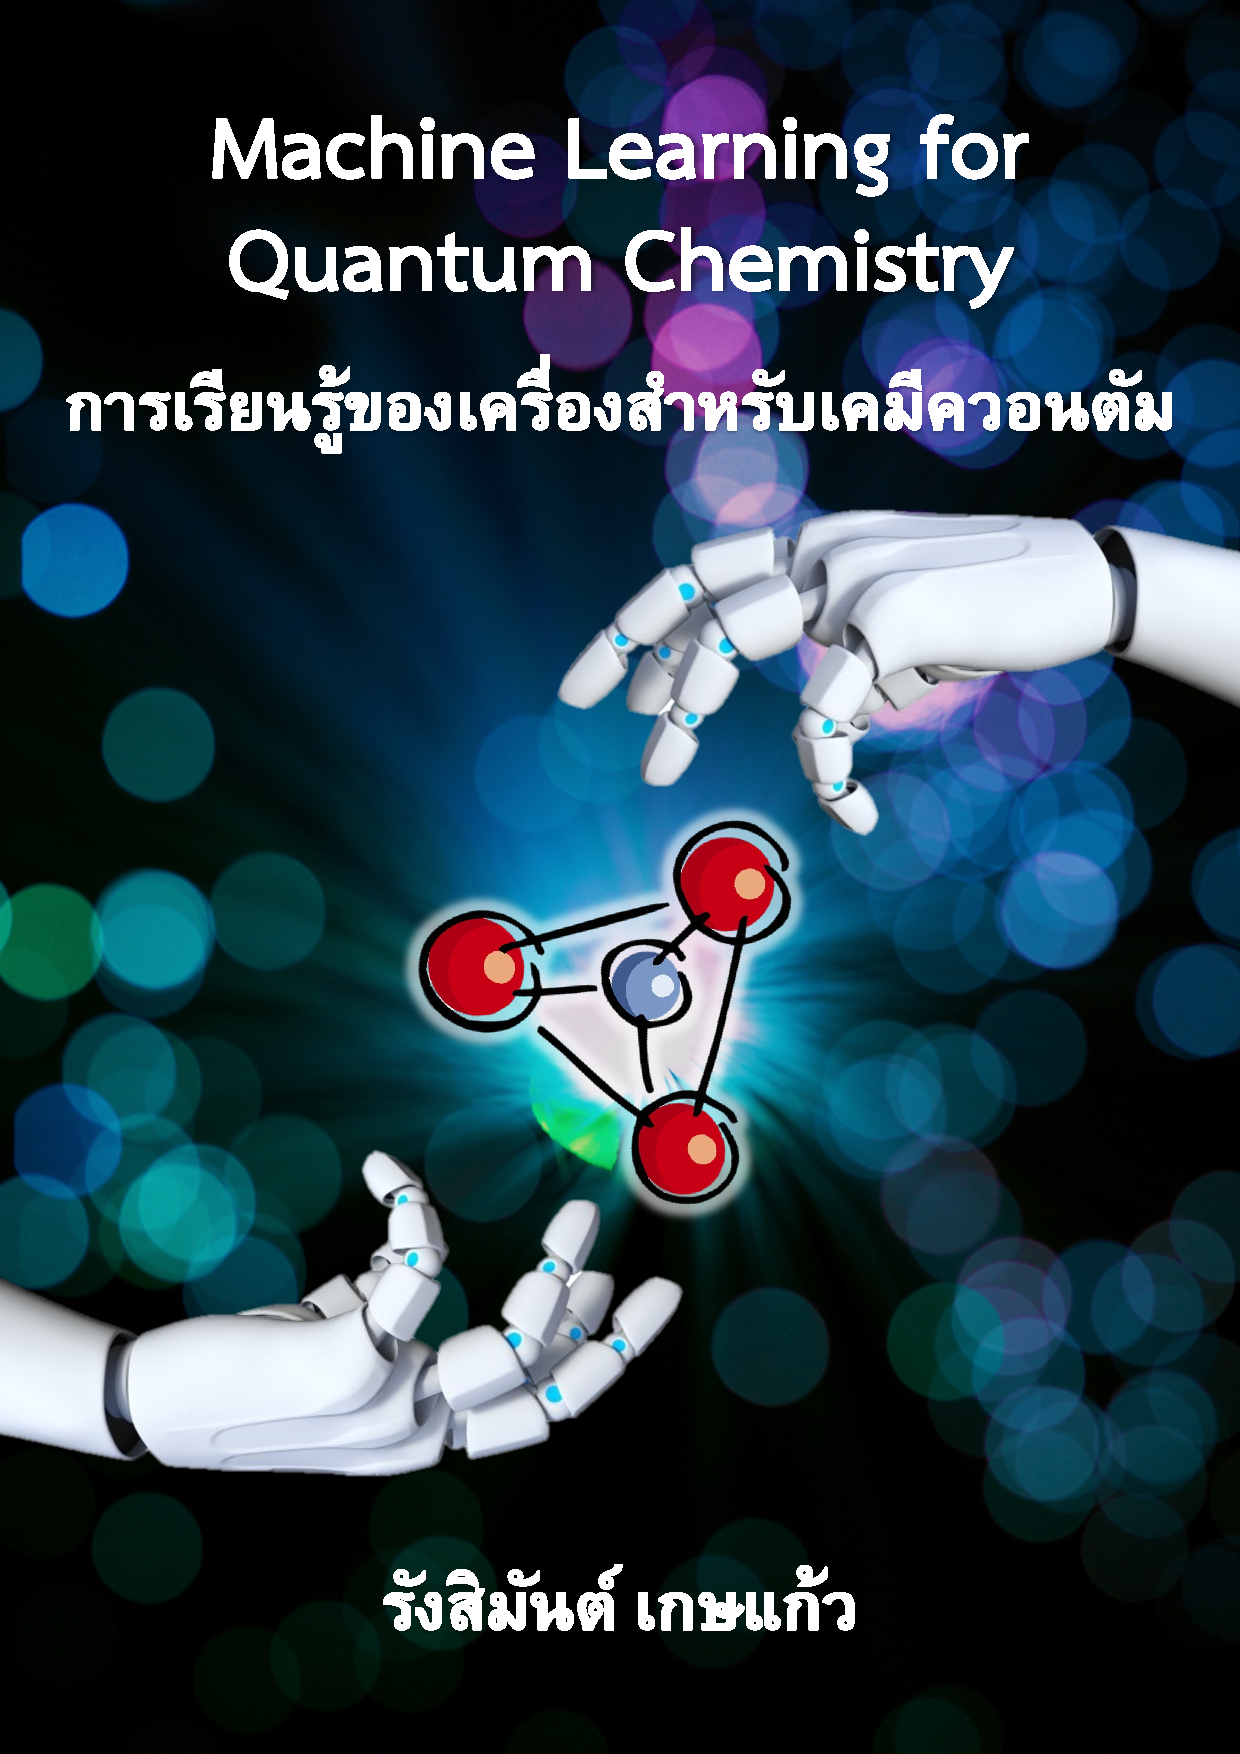
\includepdf[pages=-]{cover/cover_front.pdf}

\newpage
\ % empty page
\pagenumbering{gobble}
\newpage

\frontmatter
% LaTeX source for ``การเรียนรู้ของเครื่องสำหรับเคมีควอนตัม (Machine Learning for Quantum Chemistry)''
% Copyright (c) 2022 รังสิมันต์ เกษแก้ว (Rangsiman Ketkaew).

% License: Creative Commons Attribution-NonCommercial-NoDerivatives 4.0 International (CC BY-NC-ND 4.0)
% https://creativecommons.org/licenses/by-nc-nd/4.0/

{
\thispagestyle{empty}

\begin{flushright}
    \vspace*{2.0in}
    
    \begin{spacing}{3}
    {\Huge การเรียนรู้ของเครื่องสำหรับเคมีควอนตัม}\\
    {\LARGE Machine Learning for Quantum Chemistry}
    \end{spacing}
    
    \vspace{0.25in}
    
    {\Large รังสิมันต์ เกษแก้ว}
    
    % \date{}
    \vspace{1in}
    
    {ฉบับพิมพ์ครั้งที่ 1}
    \vspace{0.5in}
    
    %\includegraphics[width=1in]{figs/logo.pdf}
    \vfill
\end{flushright}
}

% LaTeX source for ``การเรียนรู้ของเครื่องสำหรับเคมีควอนตัม (Machine Learning for Quantum Chemistry)''
% Copyright (c) 2022 รังสิมันต์ เกษแก้ว (Rangsiman Ketkaew).

% License: Creative Commons Attribution-NonCommercial-NoDerivatives 4.0 International (CC BY-NC-ND 4.0)
% https://creativecommons.org/licenses/by-nc-nd/4.0/

{
~\vfill
\thispagestyle{empty}
\setlength{\parindent}{0em}

รังสิมันต์ เกษแก้ว

การเรียนรู้ของเครื่องสำหรับเคมีควอนตัม\\
Machine Learning for Quantum Chemistry

ปกด้านหน้า: แขนกลและโมเลกุล\\
ปกด้านหลัง: ปริภูมิเคมีของชุดข้อมูล QM9

\bigskip

\par{ฉบับพิมพ์ครั้งที่ 1 ปรับปรุงล่าสุด 21 ธันวาคม พ.ศ. 2565}

สงวนลิขสิทธิ์ตาม พ.ร.บ. ลิขสิทธิ์ พ.ศ. 2537/2540

อนุญาตให้ผู้อื่นเผยแพร่ผลงานชิ้นนี้ได้ ตราบใดที่ให้เครดิตแก่ผู้เขียนในฐานะผู้สร้างต้นฉบับและลิงก์กลับไปที่สัญญาอนุญาตของเจ้าของผลงาน 
ไม่อนุญาตให้นำไปใช้เพื่อการค้าและดัดแปลงแก้ไขไม่ว่าด้วยวิธีใด เว้นแต่จะได้รับอนุญาตเป็นลายลักษณ์อักษรจากผู้เขียน

หนังสือเล่มนี้อยู่ภายใต้ลิขสิทธิ์สัญญาอนุญาตแบบเปิด A Creative Commons Attribution-NonCommercial-NoDerivatives 4.0 
International (CC BY-NC-ND 4.0), https://creativecommons.org/licenses/by-nc-nd/4.0/.

% Use absolute path of the file

\includegraphics[scale=1.2]{front_matter/by-nc-nd.pdf}

\bigskip

ซอร์สโค้ดของหนังสือเล่มนี้ถูกเขียนขึ้นโดยใช้ภาษา {\fontfamily{lmr}\selectfont \LaTeX} เผยแพร่ที่ 
\url{https://github.com/rangsimanketkaew/ml-qm-book} และไฟล์ PDF ถูกสร้างขึ้นโดยใช้ {\fontfamily{lmr}\selectfont 
\XeLaTeX} เผยแพร่ที่ \url{https://rangsimanketkaew.github.io/ml-qm-book}

หากต้องการติดต่อผู้เขียน กรุณาส่งอีเมลมาที่ rangsiman1993[at]gmail[dot]com
}

% LaTeX source for ``การเรียนรู้ของเครื่องสำหรับเคมีควอนตัม (Machine Learning for Quantum Chemistry)''
% Copyright (c) 2022 รังสิมันต์ เกษแก้ว (Rangsiman Ketkaew).

% License: Creative Commons Attribution-NonCommercial-NoDerivatives 4.0 International (CC BY-NC-ND 4.0)
% https://creativecommons.org/licenses/by-nc-nd/4.0/

{
\pagestyle{empty} % make sure that no header on TOC pages
\tableofcontents
% \listoffigures
% \listoftables
}

% LaTeX source for ``การเรียนรู้ของเครื่องสำหรับเคมีควอนตัม (Machine Learning for Quantum Chemistry)''
% Copyright (c) 2022 รังสิมันต์ เกษแก้ว (Rangsiman Ketkaew).

% License: Creative Commons Attribution-NonCommercial-NoDerivatives 4.0 International (CC BY-NC-ND 4.0)
% https://creativecommons.org/licenses/by-nc-nd/4.0/

{
% \pagenumbering{gobble}

\chapter*{\centering คำนำ}
\addcontentsline{toc}{chapter}{คำนำ}

ในปัจจุบันได้มีการนำการเรียนรู้ของเครื่องไปใช้ประโยชน์ในหลากหลายด้าน เช่น คอมพิวเตอร์วิทัศน์, คอมพิวเตอร์กราฟฟิก, ภาษาศาสตร์, เศรษฐศาสตร์, 
อุตสาหกรรม, เกษตรกรรม รวมไปถึงวิทยาศาสตร์และวิศวกรรม โดยสาขาเคมีนั้นก็เป็นอีกหนึ่งศาสตร์ที่ได้มีการนำการเรียนรู้ของเครื่องเข้ามาประยุกต์ใช้%
มาเป็นระยะเวลานานนับตั้งแต่ช่วงปี ค.ศ. 1990 โดยนักวิจัยได้ใช้การเรียนรู้ของเครื่องในการพัฒนายาสำหรับรักษาโรค การศึกษาโครงสร้างโปรตีน 
การศึกษาคุณสมบัติของโมเลกุลและสารประกอบ การออกแบบโมเลกุลและวัสดุชนิดใหม่ รวมไปถึงการศึกษาปฏิริยาเคมีและตัวเร่งปฏิกิริยา

ผู้เขียนได้เล็งเห็นว่าการประยุกต์ใช้การเรียนรู้ของเครื่องกับเคมีควอนตัมนั้นเป็นสิ่งใหม่ที่หลายคนต่างก็ให้ความสนใจ ทั้งนักศึกษา อาจารย์ 
และนักวิจัย ดังนั้นผู้เขียนจึงได้เรียบเรียงหนังสือเล่มนี้ขึ้นมาเพื่อเป็นแนวทางให้แก่ผู้ที่ต้องการศึกษาทางด้านนี้ โดยหนังสือเล่มนี้ครอบคลุม%
ทฤษฎีและเทคนิคการเรียนรู้ของเครื่องแบบต่าง ๆ รวมไปถึงทฤษฎีเคมีควอนตัมซึ่งเป็นสาขาหนึ่งของเคมีเชิงฟิสิกส์ที่ช่วยให้เราสามารถเข้าใจองค์ความรู้%
พื้นฐานของอะตอมและโมเลกุลได้เป็นอย่างดี และหัวข้อเคมีควอนตัมที่สามารถนำการเรียนรู้ของเครื่องไปประยุกต์ใช้ได้ รวมไปถึงรายละเอียดเชิงเทคนิค%
ในการพัฒนาวิธีแบบใหม่เพื่อปรับปรุงประสิทธิภาพการพยากรณ์ของแบบจำลองการเรียนรู้ของเครื่อง

ผู้เขียนหวังเป็นอย่างยิ่งว่าหนังสือเล่มนี้จะช่วยให้ผู้อ่านทุกท่านได้รับความรู้และความเข้าใจที่ครบถ้วนเกี่ยวกับการเรียนรู้ของเครื่องสำหรับเคมีควอนตัม

\medskip

\begin{flushright}
รังสิมันต์ เกษแก้ว \\
9 ตุลาคม พ.ศ. 2565
\end{flushright}
}

% LaTeX source for ``การเรียนรู้ของเครื่องสำหรับเคมีควอนตัม (Machine Learning for Quantum Chemistry)''
% Copyright (c) 2022 รังสิมันต์ เกษแก้ว (Rangsiman Ketkaew).

% License: Creative Commons Attribution-NonCommercial-NoDerivatives 4.0 International (CC BY-NC-ND 4.0)
% https://creativecommons.org/licenses/by-nc-nd/4.0/

{
% \pagenumbering{gobble}

\chapter*{\centering กิตติกรรมประกาศ}
\addcontentsline{toc}{chapter}{กิตติกรรมประกาศ}

ความรู้และแรงบัลดาลใจในการเขียนหนังสือเล่มนี้ของผู้เขียนมาจากแรงผลักดันและการสนับสนุนของบุคคลหลายท่าน 
การเขียนหนังสือเล่มนี้จะไม่เกิดขึ้นหรือสำเร็จไม่ได้ถ้าหากขาดบุคคลดังต่อไปนี้

ครอบครัวของผู้เขียนที่สนับสนุนให้ผู้เขียนได้ทำตามความฝันในการเรียนต่อระดับอุดมศึกษา ทั้งในระดับปริญญาโทและปริญญาเอก 
โดยเฉพาะการเห็นคุณค่าของการเรียนและการทำงานวิจัยทางด้านวิทยาศาสตร์พื้นฐาน

รศ.ดร. ยุทธนา ตันติรุ่งโรจน์ชัย บุคคลผู้เป็นต้นแบบด้านการเรียนและเป็นผู้สร้างแรงบันดาลใจให้ผู้เขียนเรียนต่อต่างประเทศและทำงานวิจัยทางด้าน%
เคมีทฤษฎีและเคมีคอมพิวเตอร์

อาจารย์และเพื่อน ๆ ในช่วงมัธยมศึกษา (ตอนต้น-ปลาย) ที่โรงเรียนพนัสพิทยาคาร และช่วงปริญญาตรี-โท ที่มหาวิทยาลัยธรรมศาสตร์ 
สำหรับความทรงจำอันดีงามและความเป็นกัลยาณมิตรที่ดีเสมอมา

เพื่อน ๆ ที่เมืองซูริค ประเทศสวิตเซอร์แลนด์ สำหรับมิตรภาพอันดีงาม รอยยิ้มและเสียงหัวเราะที่เกิดขึ้น รวมไปถึงกิจกรรมที่ได้ทำร่วมกันในระหว่าง%
ที่ผู้เขียนกำลังศึกษาปริญญาเอกซึ่งเป็นช่วงเวลาเดียวกันกับที่ผู้เขียนกำลังเขียนหนังสือเล่มนี้

เพื่อนร่วมงานทั้งนักศึกษาปริญญาโท ปริญญาเอก และนักวิจัยหลังปริญญาเอกของกลุ่มวิจัยของผู้เขียนที่ภาควิชาเคมี
มหาวิทยาลัยแห่งซูริค สำหรับการแลกเปลี่ยนความรู้ ไอเดียใหม่ ๆ และการช่วยเหลือเกี่ยวกับงานวิจัยทางด้านเคมีทฤษฎี

\medskip

\begin{flushright}
รังสิมันต์ เกษแก้ว
\end{flushright}
}

% LaTeX source for ``การเรียนรู้ของเครื่องสำหรับเคมีควอนตัม (Machine Learning for Quantum Chemistry)''
% Copyright (c) 2022 รังสิมันต์ เกษแก้ว (Rangsiman Ketkaew).

% License: Creative Commons Attribution-NonCommercial-NoDerivatives 4.0 International (CC BY-NC-ND 4.0)
% https://creativecommons.org/licenses/by-nc-nd/4.0/

{
% \pagenumbering{gobble}

\chapter*{\centering คำแนะนำในการอ่านหนังสือเล่มนี้}
\addcontentsline{toc}{chapter}{คำแนะนำในการอ่านหนังสือเล่มนี้}

ผู้เขียนเรียบเรียงหนังสือเล่มนี้ขึ้นมาเพื่อเป็นแหล่งความรู้สำหรับบุคคลที่สนใจการเรียนรู้ของเครื่องสำหรับเคมีควอนตัม เนื่องจากว่าในปัจจุบันนั้นยังไม่มี%
หนังสือเฉพาะทางสำหรับการทำงานวิจัยในสาขานี้ ดังนั้นหนังสือเล่มนี้จึงไม่ได้ถูกแปลมาจากหนังสือหรือตำราต่างประเทศ แต่มาจากการอ่านและสรุป%
จากบทความงานวิจัยที่ตีพิมพ์ในวารสารวิชาการชั้นนำทางด้านปัญญาประดิษฐ์และเคมีทฤษฎีที่ได้รับการยอมรับ แล้วเรียบเรียงใหม่ตามความเข้าใจของ%
ผู้เขียน

หนังสือเล่มนี้จะเน้นไปที่การอธิบายทฤษฏีประกอบกับสมการทางคณิตศาสตร์อย่างกระชับ โดยผู้เขียนใช้สำนวนที่ไม่เป็นทางการมากนักและพยายามอธิบาย%
ความหมายของคำศัพท์เฉพาะทางเพื่อให้ผู้อ่านสามารถเข้าใจเนื้อหาที่ซับซ้อนได้ง่ายขึ้น ดังนั้นสไตล์การเขียนของผู้เขียนจะเป็นในเชิงที่ใช้ภาษาพูด โดยมี%
การใส่ความคิดเห็นส่วนตัว แนวคิดและมุมมองของผู้เขียนที่ได้จากการอภิปรายกับเพื่อนร่วมงานและผู้เชี่ยวชาญในสาขาที่คิดว่าเหมาะสมเข้าไปด้วย

หนังสือเล่มนี้ประกอบไปด้วยเนื้อหาสามส่วน ดังนี้ 

\begin{enumerate}[topsep=0pt]
    \item \textbf{การเรียนรู้ของเครื่อง}: ในส่วนแรกผู้อ่านจะได้ศึกษาที่มาและความสำคัญของการเรียนรู้ของเครื่องและการเชื่อมโยงเพื่อนำไป%
    ใช้กับเคมีควอนตัม โดยเฉพาะในการทำงานวิจัย ผู้อ่านจะได้ศึกษาอัลกอริทึมต่าง ๆ ของการเรียนรู้ของเครื่องทั้งการเรียนรู้แบบมีผู้สอนและแบบไม่มี%
    ผู้สอนซึ่งเป็นอัลกอริทึมมาตรฐานที่นักวิจัยใช้เพื่อพัฒนาโมเดลสำหรับการทำนายเอาต์พุตที่ต้องการ นอกจากนี้ผู้อ่านจะได้เรียนรู้ปัญหาของการเรียนรู้%
    ของเครื่องที่มักจะพบเจอได้บ่อยและขั้นตอนหรือเทคนิคการแก้ปัญหาดังกล่าว และการเลือกโมเดลการเรียนรู้ของเครื่องเพื่อให้เหมาะสมกับโจทย์ทาง%
    สถิติที่ต้องการแก้
    
    \item \textbf{การทำนายคุณสมบัติเชิงเคมีควอนตัม}: ในส่วนที่สองจะเป็นการอธิบายทฤษฎีของโครงสร้างเชิงอิเล็กทรอนิกส์ (Electronic 
    Structure) ของอะตอมและโมเลกุล นอกจากนี้ผู้อ่านจะได้ศึกษาชุดข้อมูลทางเคมีควอนตัม ทฤษฎีของคุณสมบัติเชิงโมเลกุลแบบต่าง ๆ ซึ่งเป็น%
    สิ่งที่นักวิจัยเคมีทฤษฎีให้ความสนใจและเกี่ยวข้องโดยตรงกับหัวข้อถัดไปนั่นก็คือทฤษฎีของตัวอธิบายเชิงอิเล็กทรอนิกส์ (Electronic-based 
    Descriptor) แบบต่าง ๆ ที่ได้รับการพัฒนาตั้งแต่อดีตจนถึงปัจจุบันและถูกนำมาใช้สำหรับการคำนวณลักษณะเฉพาะ (Feature) ของโมเลกุล 
    เมื่อศึกษา Feature ที่เราจะนำมาใช้เป็นอินพุตสำหรับการฝึกสอนโมเดลแล้ว ผู้อ่านจะได้ศึกษาการสร้างและพัฒนาโมเดลการเรียนรู้ของเครื่องรวม%
    ไปถึงโมเดลเฉพาะทางแบบต่าง ๆ ที่ได้รับการพัฒนาในช่วงสิบปีที่ผ่านมา และการวิเคราะห์ผลการทำนายของโมเดลซึ่งจะเป็นประโยชน์ในการทำงาน%
    วิจัยและการตีพิมพ์ต่อไป

    \item \textbf{ภาคผนวก}: ในส่วนที่สามเป็นภาคผนวกซึ่งจะรวบรวมหัวข้อพื้นฐานที่เป็นประโยชน์ต่อการทำความเข้าใจเนื้อหาหลักในสองส่วน%
    แรก ประกอบไปด้วยพื้นฐานพีชคณิตเชิงเส้นซึ่งเกี่ยวข้องกับเมทริกซ์ การเขียนโปรแกรมสำหรับปัญญา ประดิษฐ์โดยผู้อ่านจะได้ฝึกการเขียนโปรแกรม%
    ของโครงข่ายประสาท (Neural Network) ด้วยไลบรารี่ TensorFlow เป็นต้น นอกจากนี้ยังมีการอธิบายเกี่ยวกับโปรแกรมเคมีเชิงคำนวณที่%
    ผู้อ่านสามารถใช้งานเพื่อคำนวณคุณสมบัติเชิงโครงสร้างและอิเล็กทรอนิกส์ของโมเลกุลได้อีกด้วย
\end{enumerate}

ในการอธิบายตัวทฤษฎีนั้นผู้เขียนได้พยายามใส่โค้ดของโปรแกรมที่ผู้อ่านสามารถนำไปเขียนตามและลองรันได้ด้วยตนเองเข้าไปด้วย ซึ่งจากประสบการณ์%
ส่วนตัวของผู้เขียนพบว่าการเขียนโปรแกรมนั้นสามารถช่วยให้เราเข้าใจทฤษฎีต่าง ๆ ทางเคมีได้อย่างเป็นขั้นเป็นตอน รวมไปถึงเข้าใจวิธีคิดสำหรับการ%
คำนวณปริมาณต่าง ๆ ทางฟิสิกส์และเคมี ดังนั้นผู้เขียนจึงแนะนำให้ผู้อ่านศึกษาโค้ดอย่างละเอียดและไม่ควรข้ามไป

\medskip

\begin{flushright}
รังสิมันต์ เกษแก้ว
\end{flushright}
}

% LaTeX source for ``การเรียนรู้ของเครื่องสำหรับเคมีควอนตัม (Machine Learning for Quantum Chemistry)''
% Copyright (c) 2022 รังสิมันต์ เกษแก้ว (Rangsiman Ketkaew).

% License: Creative Commons Attribution-NonCommercial-NoDerivatives 4.0 International (CC BY-NC-ND 4.0)
% https://creativecommons.org/licenses/by-nc-nd/4.0/

{
\thispagestyle{empty}
~\vfill

\begin{doublespace}
\noindent\fontsize{16}{22}\selectfont\itshape
\nohyphenation
If I have seen further, it is by standing on the shoulders of Giants.\\
\noindent - \mbox{Sir Isaac Newton PRS} (1643 - 1726)
\end{doublespace}

\vfill
\vfill
}


\pagestyle{fancy} % Add header from this page on

\mainmatter
\part{การเรียนรู้ของเครื่อง}
% LaTeX source for ``การเรียนรู้ของเครื่องสำหรับเคมีควอนตัม (Machine Learning for Quantum Chemistry)''
% Copyright (c) 2022 รังสิมันต์ เกษแก้ว (Rangsiman Ketkaew).

% License: Creative Commons Attribution-NonCommercial-NoDerivatives 4.0 International (CC BY-NC-ND 4.0)
% https://creativecommons.org/licenses/by-nc-nd/4.0/

\chapter{การเรียนรู้ของเครื่อง}
\label{ch:ml}

\idxboth{การเรียนรู้ของเครื่อง}{Machine Learning}
\idxboth{การฝึกสอนโมเดล}{Model Training}

%--------------------------
\section{ความสำคัญของการเรียนรู้ของเครื่อง}
\label{sec:why_ml}
%--------------------------

\begin{figure}[H]
    \centering
    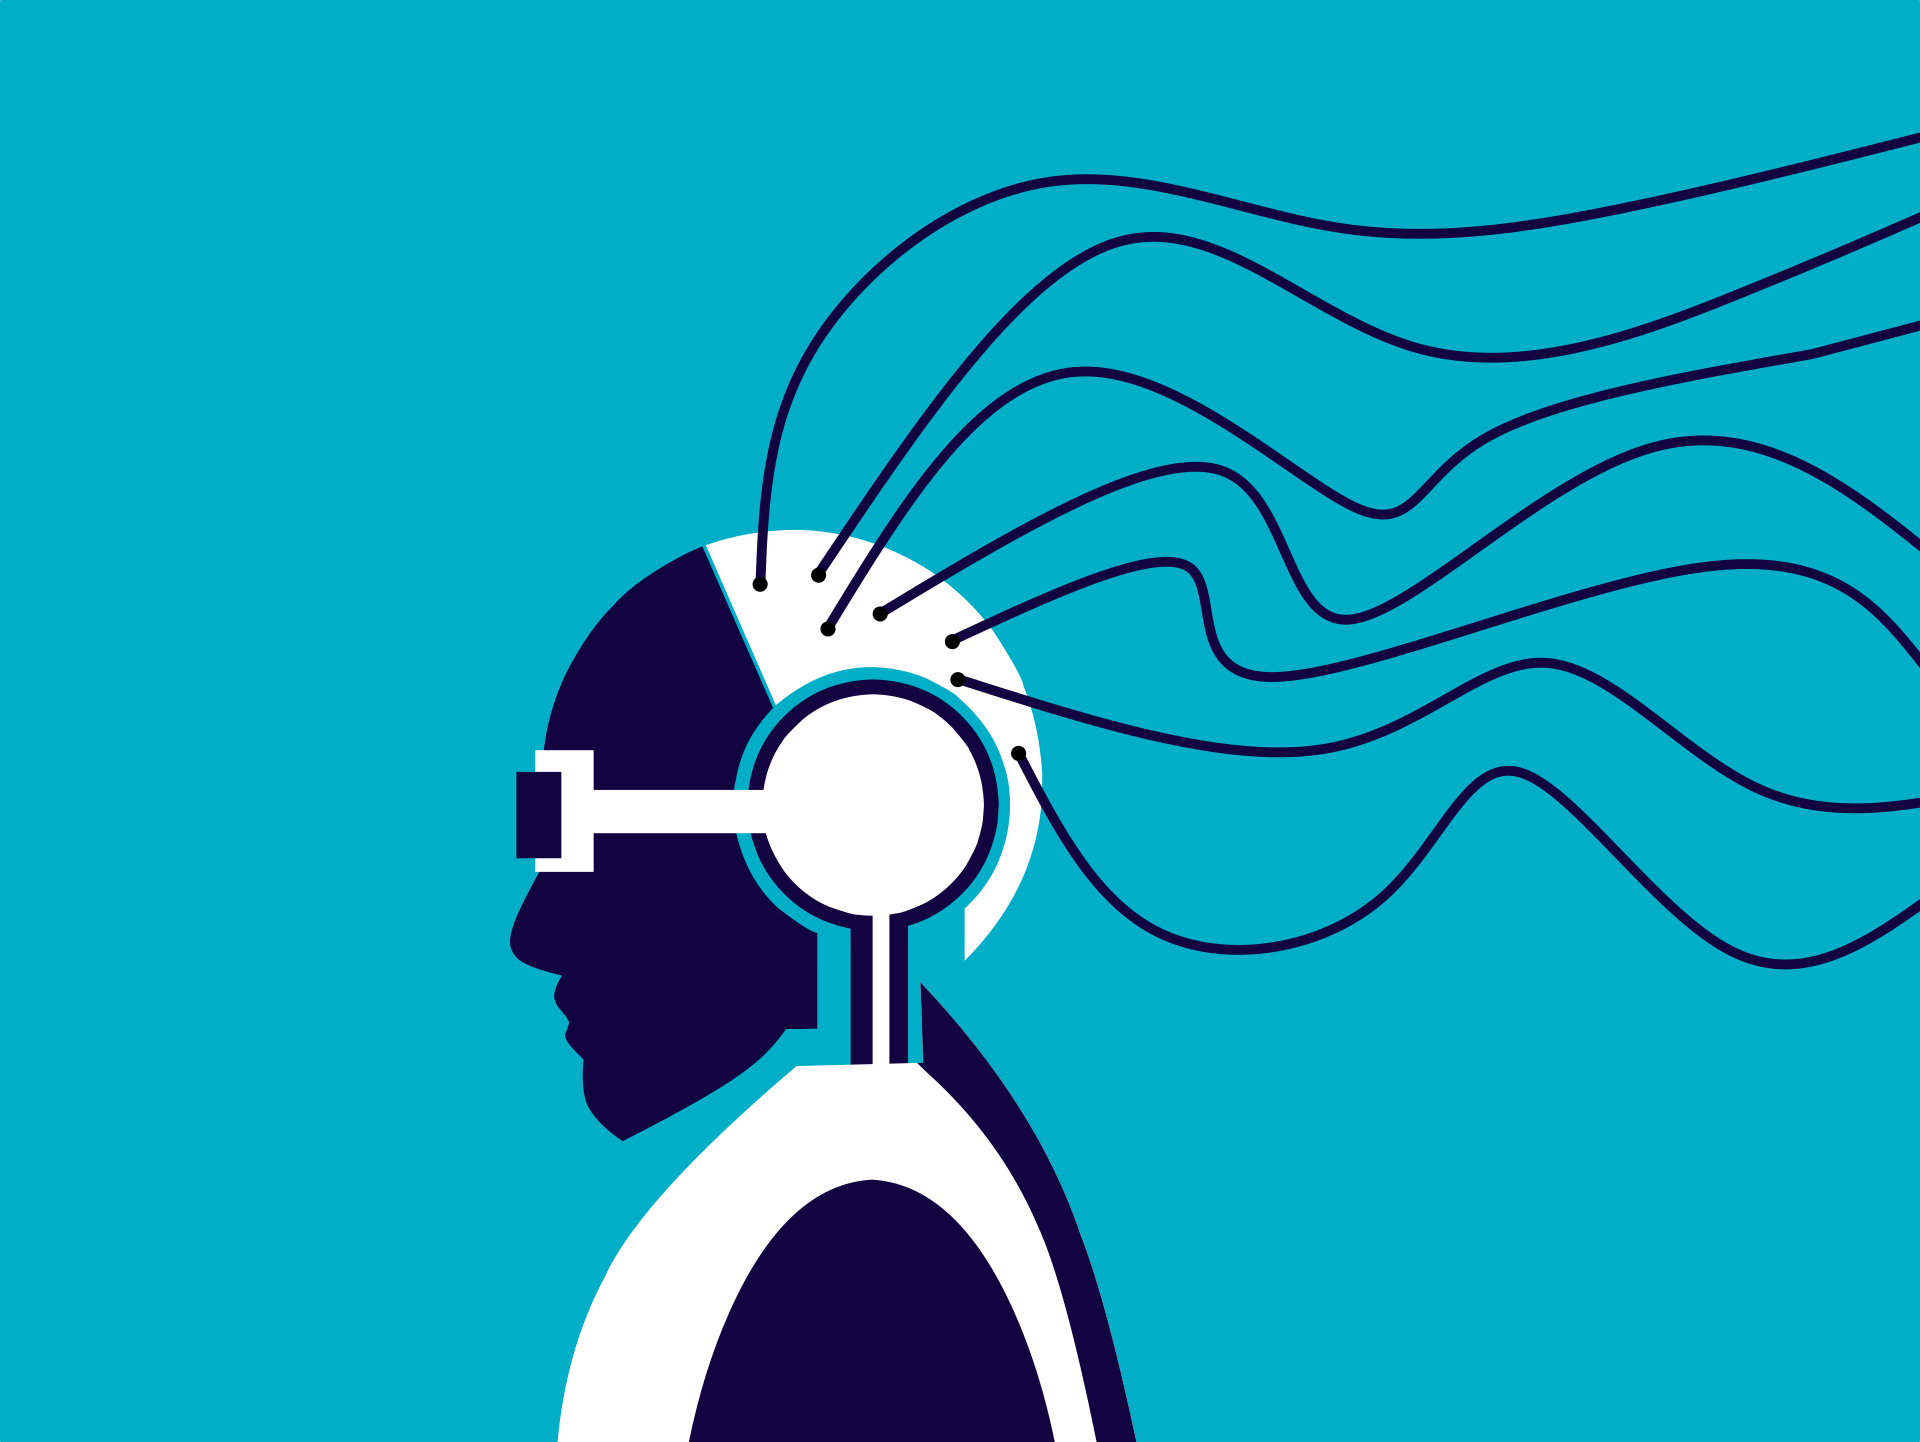
\includegraphics[width=0.8\linewidth]{fig/cyborg.png}
    \caption{ภาพแสดงหุ่นยนต์ที่มีสมองที่มีความนึกคิดและสติปัญญา (เครดิตภาพ: https://pixabay.com)}
    \label{fig:cyborg}
\end{figure}

การเรียนรู้ของเครื่อง (Machine Learning หรือ ML) เป็นศาสตร์ที่เชื่อมโยงวิชาสถิติ คณิตศาสตร์ และวิทยาการคอมพิวเตอร์เข้าด้วยกัน
อธิบายง่าย ๆ คือมนุษย์พยายามทำให้เครื่องจักรนั้นมี \enquote{สติปัญญา} หรือ \enquote{ความฉลาด} และมีความสามารถในการเรียนรู้สิ่งต่าง ๆ 
ได้ด้วยตัวเอง โดยกระบวนการดังกล่าวนั้นจะเกี่ยวข้องกับการฝึกสอนเครื่องจักรจนกระทั่งเครื่องจักรสามารถเรียนรู้และค่อย ๆ พัฒนาการทำงานต่าง ๆ 
ได้โดยไม่ต้องพึ่งการตั้งโปรแกรม ซึ่งในบริบทนี้เครื่องจักรที่เรารู้จักกันดีก็คืออุปกรณ์ที่มีหน่วยประมวลผล (Processing Unit) เช่น คอมพิวเตอร์ 
ที่ถูกสั่งงานหรือควบคุมผ่านซอฟต์แวร์ในรูปแบบของโปรแกรมนั่นเอง โดยวิธีการก็คือเราป้อนข้อมูลเข้าไปให้กับโปรแกรม โปรแกรมจะทำการสร้างโมเดล
(Model) ที่สามารถอธิบายความสัมพันธ์ในข้อมูลที่เราป้อนเข้าไปได้ ซึ่งขั้นตอนที่เกิดขึ้นระหว่างการเรียนรู้ก็คือการฝึกสอนโมเดล (Model Training) 
ซึ่งโปรแกรมสามารถแปลงข้อมูลทั้งหมดเป็นโมเดลที่ปรับปรุงได้ นั่นหมายความว่าเทคโนโลยี ML สามารถทำให้คอมพิวเตอร์เรียนรู้วิธีทำงานของมนุษย์ได้
โดยเฉพาะการลอกเลียนแบบ (Imitation) กิจกรรมที่ทำซ้ำหรือเกิดขึ้นแบบเดิมจนมีแบบแผน (Pattern) ยกตัวอย่างเช่น ถ้าเรามีข้อมูล 2 ตัวแปร 
$(x,y)$ เราใช้ ML เพื่อหาฟังก์ชันที่สามารถเชื่อมโยง (Correlate) ความสัมพันธ์ระหว่างสองตัวแปรนี้ได้ $f: x\rightarrow y$

ML ได้ถูกพัฒนาเรื่อยมาเป็นระยะเวลาหลายทศวรรษ จุดเริ่มต้นที่นับได้ว่าสำคัญที่สุดของปัญญาประดิษฐ์เกิดขึ้นในปี ค.ศ. 1943 โดยนักตรรกศาสตร์
Walter Pitts และนักประสาทวิทยา Warren McCulloch ได้ตีพิมพ์ผลงานที่เสนออัลกอริทึมคณิตศาสตร์ของโครงข่ายประสาท (Neural Network) 
และในปี ค.ศ. 1950 นักคณิตศาสตร์และนักถอดรหัสชื่อดัง Alan Turing\footnote{Alan Turing เป็นอัจฉริยะด้านคณิตศาสตร์และการคำนวณ 
จบการศึกษาปริญญาตรีจาก University of Cambridge และปริญญาเอกจาก Princeton University โดยในช่วงสงครามโลก Alan 
ได้สร้างเครื่องถอดรหัสที่ชื่อว่า Bombe เพื่อมาต่อสู้กับเครื่อง Enigma ซึ่งได้การประเมินไว้ว่าผลงานของ Alan ได้ช่วยชีวิตไว้ได้หลายล้านคน} 
ได้เสนอการทดสอบของทัวริง (The Turing Test)\autocite{turing1950} ซึ่งเป็นแนวคิดในการทดสอบความมีสติปัญญาของเครื่องจักร 
โดยหนึ่งในการทดสอบอันโด่งดังก็คือเกมเลียนแบบ (Imitation Game)\footnote{ผู้อ่านสามารถอ่านบทความงานวิจัยต้นฉบับของ Alan Turing 
ได้ที่ \url{https://academic.oup.com/mind/article/LIX/236/433/986238} หรือดูภาพยนต์เรื่อง The Imitation Game} 
หลังจากนั้นได้มีเหตุการณ์สำคัญเกิดขึ้นอีกมากมาย เช่น Arthur Samuel ได้เขียนโปรแกรมเล่นหมากฮอสโปรแกรมแรกของโลกให้กับ IBM 
ในปี ค.ศ. 1952 และอัลกอริทึม Nearest Neighbor ถูกคิดค้นขึ้นในช่วงปี ค.ศ. 1967 และในปี ค.ศ. 1996 IBM ได้พัฒนาโปรแกรมที่ชื่อว่า 
Deep Blue ที่สามารถเอาชนะนักหมากรุกมือวางอันดับหนึ่งของโลกได้สำเร็จ

\begin{figure}[H]
    \centering
    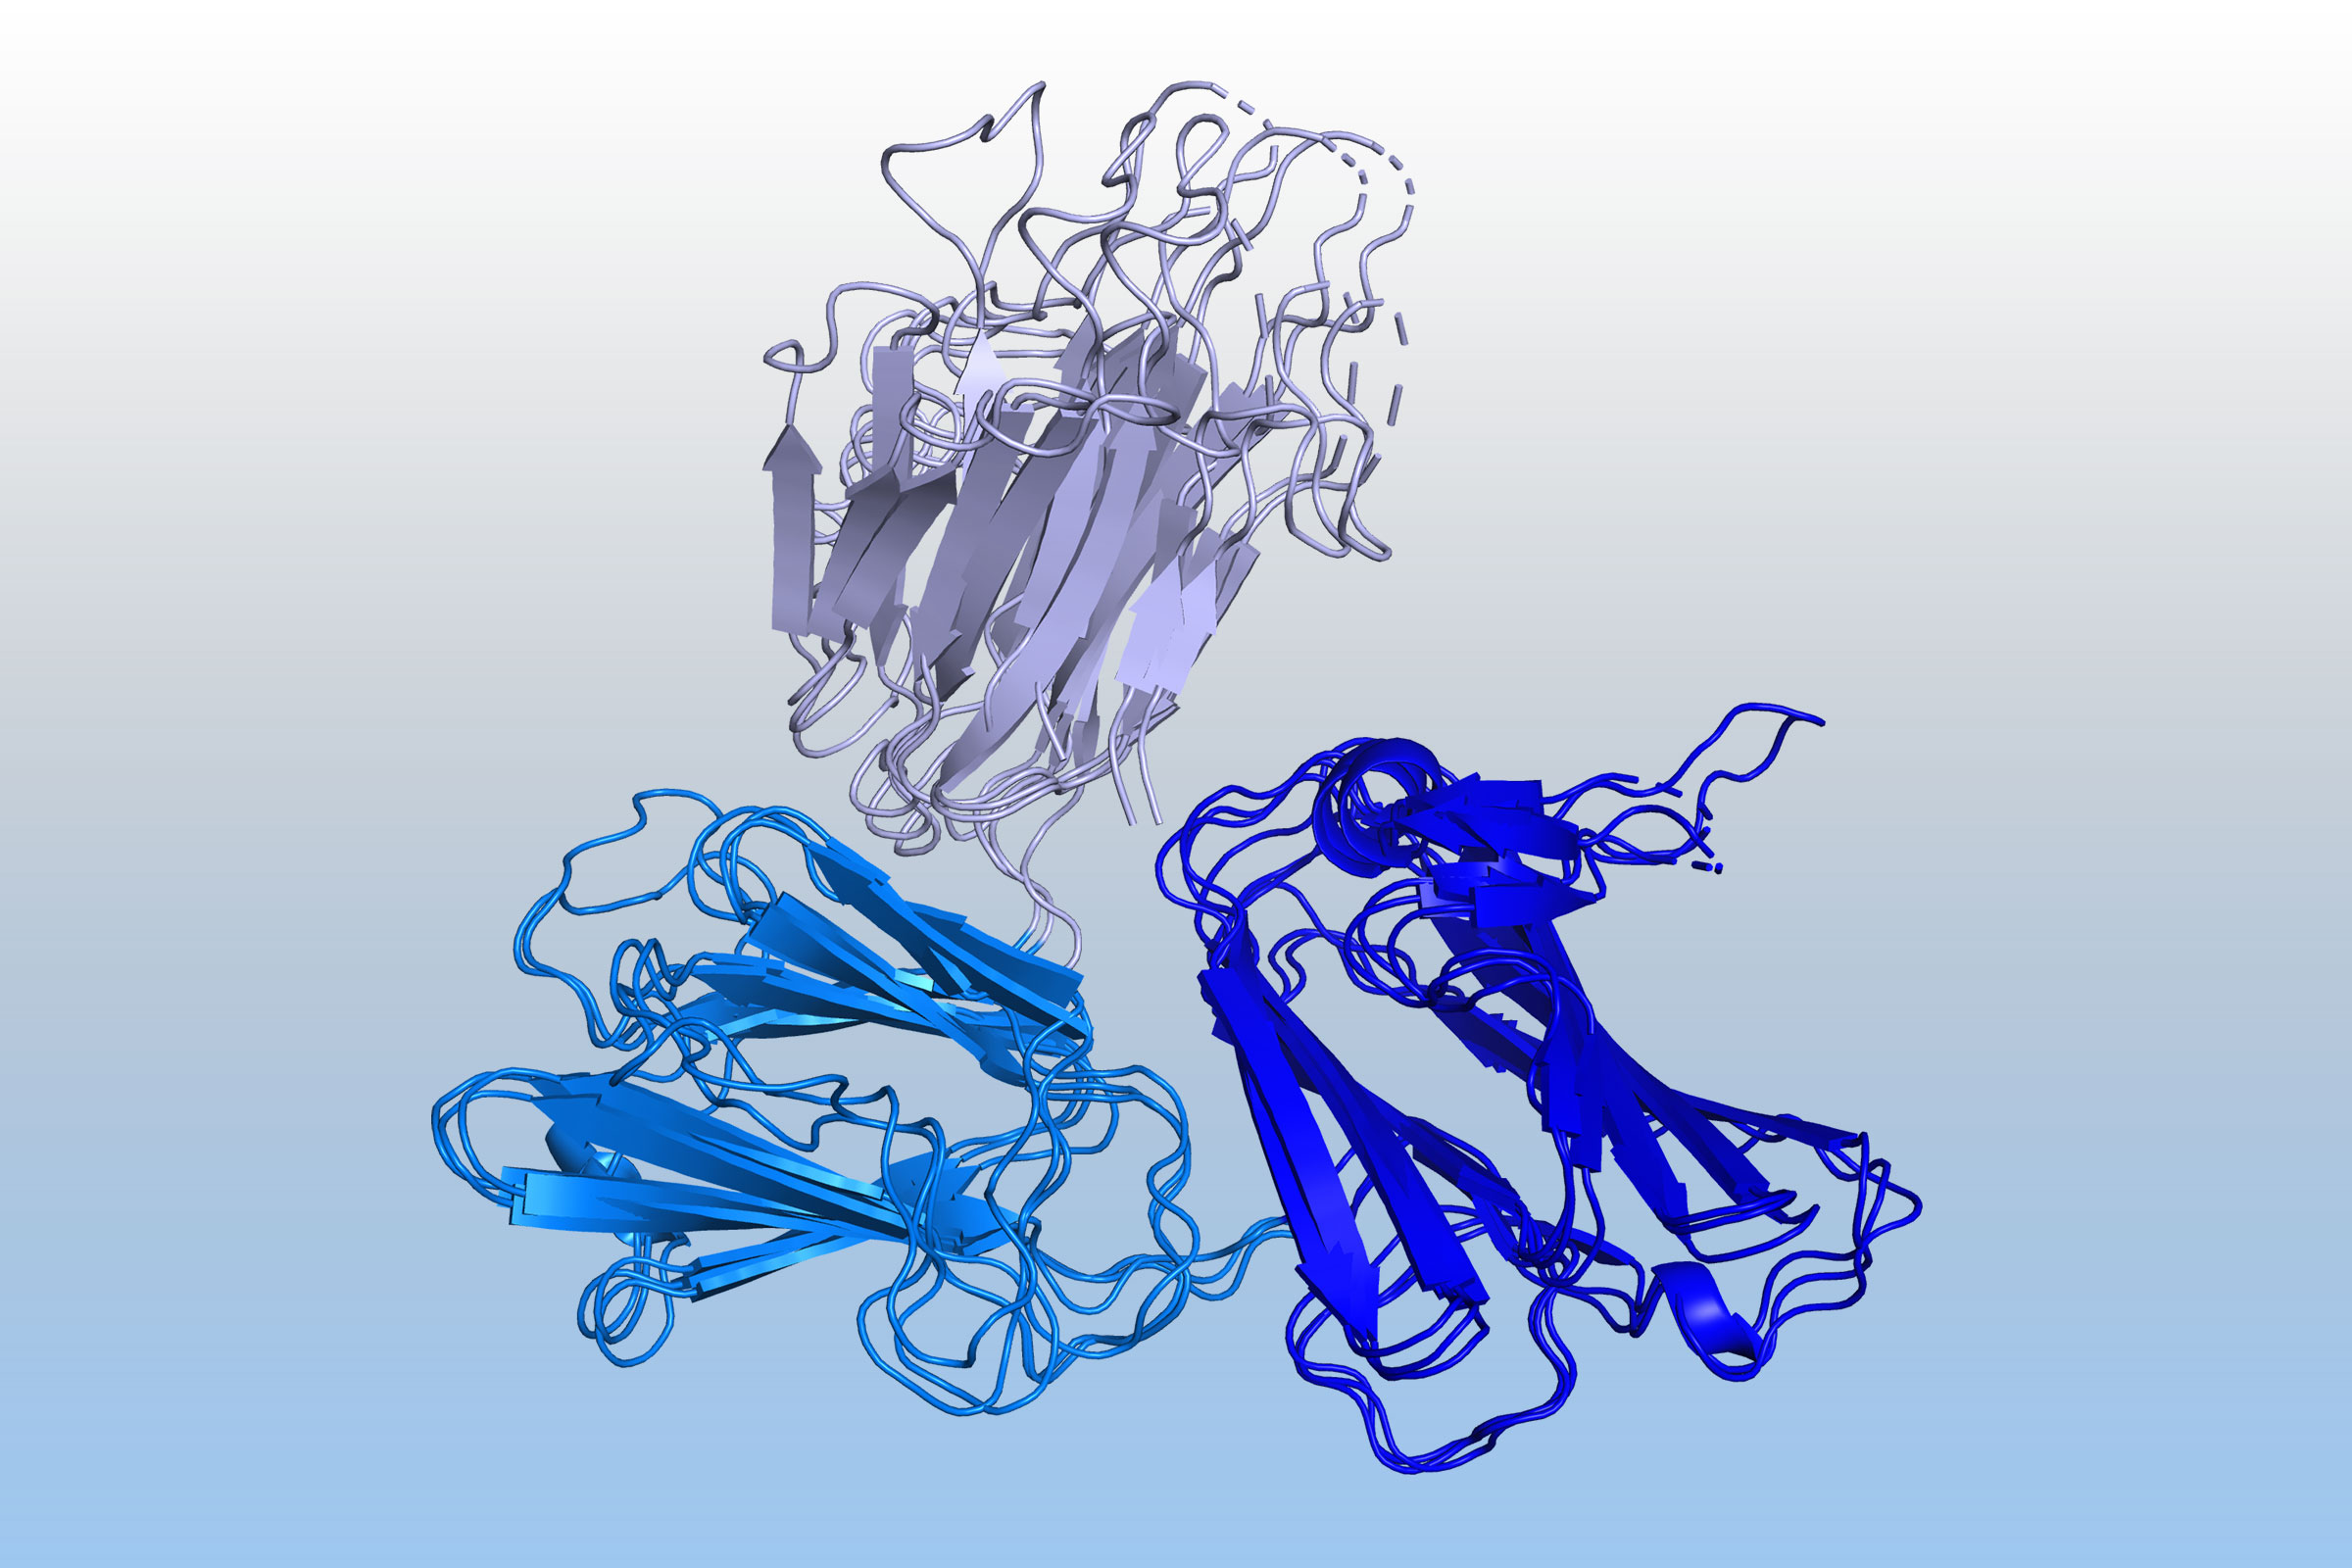
\includegraphics[width=\linewidth]{fig/malaria-parasite-protein-deepmind.jpeg}
    \caption{แบบจำลองโครงสร้างสามมิติการพับของโปรตีน Pfs48/45 ซึ่งเป็นองค์ประกอบสำคัญของปรสิตมาลาเรีย โครงสร้างนี้ทำนายด้วยโมเดล 
    ปัญญาประดิษฐ์ AlphaFold ซึ่งถูกพัฒนาโดย DeepMind (เครดิตภาพ: DeepMind)}
    \label{fig:malaria_parasite}
\end{figure}

นับตั้งแต่ปี ค.ศ. 2000 เป็นต้นมานั้นเรียกได้ว่าเป็นช่วงของการพัฒนาปัญญาประดิษฐ์แบบสมัยใหม่ก็ว่าได้ จุดเปลี่ยนที่น่าสนใจที่ทำให้คนหันมาสนใจ%
และให้ความสำคัญกับ ML ก็คือในช่วงระยะเวลา 10 ปีที่ผ่านมาได้มีเหตุการณ์สำคัญที่สร้างแรงกระเพื่อมแก่มวลมนุษยชาติ เช่น ในปี ค.ศ. 2011 
Apple ได้ปล่อยผลิตภัณฑ์ที่ชื่อ Siri ซึ่งเป็นผู้ช่วยเสมือน (Intelligent Virtual Assistant) อันแสนฉลาดออกมา และในปี ค.ศ. 2016 
บริษัท DeepMind ซึ่งเป็นบริษัทลูกของ Alphabet ก็พัฒนาโมเดลปัญญาประดิษฐ์ AlphaGo ที่สามารถเล่นหมากล้อมได้อย่างชาญฉลาด 
และก็เป็นปีเดียวกันกับที่ DeepMind ได้เริ่มต้นพัฒนา AlphaFold ซึ่งเป็นโมเดล ML สำหรับการทำนายโครงสร้างสามมิติของโปรตีน และในปี ค.ศ. 
2021 DeepMind ก็ได้ตีพิมพ์บทความที่นำเสนอ AlphaFold 2 ออกมาครับ\autocite{jumper2021} 
\footnote{
\setlength\intextsep{0pt}
\begin{wrapfigure}{r}{0.2\textwidth}
        \centering
        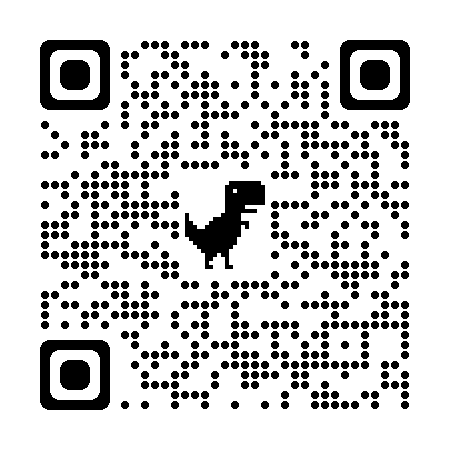
\includegraphics[width=0.18\textwidth]{fig/qr_code_alphafold2_explained.png}
\end{wrapfigure}
ถ้าหากอ่านบทความแล้วยังไม่เข้าใจก็สามารถดูวิดีโอบน YouTube \enquote{DeepMind's AlphaFold 2 Explained! 
AI Breakthrough in Protein Folding! What we know (\& what we don't)} ที่อธิบายโดย Yannic Kilcher ได้โดยสแกน 
QR Code ทางด้านขวา}

ช่วงปลายปี ค.ศ. 2022 ทีม DeepMind ก็ได้สะเทือนวงการปัญญาประดิษฐ์อีกครั้งด้วยอัลกอริทึม ML แบบใหม่ที่สามารถหาอัลกอริทึมที่สามารถคูณ%
เมทริกซ์ได้โดยมีความเร็วมากกว่าอัลกอริทึมแบบดั้งเดิมที่ใช้กันมายาวนานกว่า 50 ปี โดยโมเดล ML ที่ทาง DeepMind ได้สร้างขึ้นมานั้นมีชื่อว่า 
AlphaTensor โดยใช้ Transformer\autocite{vaswani2017} เป็นโมเดลหลักในการฝึกสอน\footnote{โมเดลการเรียนรู้เชิงลึกแบบหนึ่งซึ่งใช้ 
Self-attention พัฒนาโดย Google Brain สำหรับงานทางด้านการประมวลผลภาษาธรรมชาติ (Natural Language Processing) หรือ 
NLP และเผยแพร่ในปี ค.ศ. 2017} โดยอัลกอริทึม ML ที่ถูกค้นพบโดย AlphaTensor สามารถทำการคูณเมทริกซ์ขนาด $4 \time 4$ 
ได้โดยใช้การคูณทั้งหมดแค่ 47 ครั้ง ซึ่งน้อยกว่าการใช้อัลกอริทึมของสตราซเซนแบบสองระดับ (Strassen's Two-level Algorithm) 
ซึ่งใช้การคูณทั้งหมด 49 ครั้ง\autocite{strassen1969}  และค่าความซับซ้อนเชิงการคำนวณ (Computational Complexity) 
ของอัลกอริทึมใหม่นี้อยู่ที่ประมาณ ${\mathcal{O}}({N}^{2.778})$ 

จากตัวอย่างข้างต้นนั้นเราสามารถสรุปได้อย่างไม่ต้องลังเลเลยว่า ML นั้นสามารถปฏิวัติวงการต่าง ๆ ได้อย่างน่าเหลือเชื่อ ไม่เพียงเฉพาะวงการ%
คณิตศาสตร์และวิทยาศาสตร์เท่านั้น แต่รวมไปถึงวงการอื่น ๆ ด้วยที่เทคนิคเหล่านี้เข้าไปมีบทบาท ซึ่งไม่เพียงแค่ในเฉพาะปัจจุบันเท่านั้นแต่ว่าใน%
อนาคตนั้นเราอาจจะได้เห็นสิ่งใหม่ ๆ ที่ ML นั้นสามารถสร้างสรรค์ขึ้นมาได้เอง

\begin{figure}[H]
    \centering
    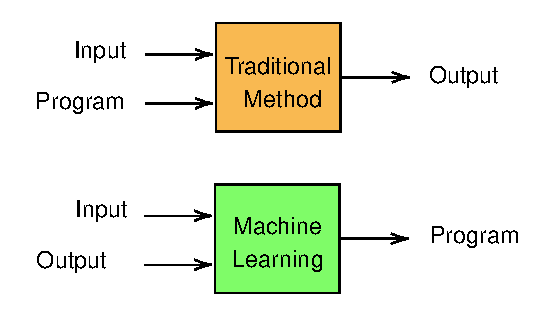
\includegraphics[scale=1]{fig/ML-concept.pdf}
    \caption{แผนภาพเปรียบเทียบการทำงานของโปรแกรมแบบดั้งเดิมกับการเรียนรู้ของเครื่อง}
    \label{fig:ml_paradigm}
\end{figure}

แผนภาพที่ \ref{fig:ml_paradigm} แสดงการเปรียบเทียบอินพุต (Input) และเอาต์พุต (Output) ระหว่างโปรแกรมคอมพิวเตอร์ทั่วไปแบบ%
ดั้งเดิมที่เราเขียนโค้ดกันอยู่ในทุกวันนี้และโมเดลของปัญญาประดิษฐ์ โดยการเขียนโปรแกรมแบบทั่วไปนั้นเราจะต้องทำการเขียนโปรแกรมเริ่มต้นขึ้นมา%
และทำการป้อนอินพุตเข้าไปเพื่อให้ได้มาซึ่งเอาต์พุตหรือคำตอบที่เราต้องการ โดยกระบวนการของการเขียนโปรแกรมแบบดั้งเดิมนั้นจะเป็นกระบวนการ%
แบบที่ทำแล้วจบ อธิบายง่าย ๆ คือโปรแกรมของเราถูกกำหนดมาเพื่อรับอินพุตและคำนวณเอาต์พุตรูปแบบเดียว ซึ่งเราไม่สามารถนำโปรแกรมที่เขียน%
ขึ้นมานี้ไปใช้ต่อได้ (Non-transferable) แต่สำหรับกรณีของปัญญาประดิษฐ์หรือ ML นั้นจะตรงข้ามกันนั่นคือเราจะมีการป้อนทั้งอินพุตและเอาต์พุต%
เข้าไปให้กับปัญญาประดิษฐ์แล้วให้ปัญญาประดิษฐ์ทำการสร้างโปรแกรมหรือโมเดลโดยใช้เทคนิค ML ที่สามารถอธิบายความสัมพันธ์ของชุดข้อมูลที่มี%
ตัวแปรต้นหรือตัวแปรอิสระ (Independent Variable) และตัวแปรตาม (Dependent Variable) ได้ ซึ่งโมเดล ML ที่ถูกสร้างขึ้นมานี้สามารถ%
นำไปใช้งานต่อกับชุดข้อมูลอื่นได้ เราเรียกความสามารถนี้ของโมเดลว่าความสามารถในการส่งต่อหรือส่งผ่าน (Transferability)

%--------------------------
\section{เมื่อการเรียนรู้ของเครื่องมาเจอกับเคมี}
\label{sec:ml_meets_chem}
%--------------------------

\begin{figure}[H]
    \centering
    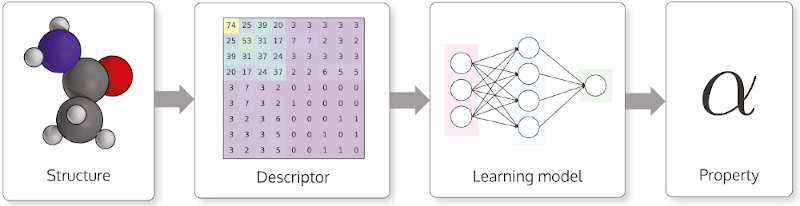
\includegraphics[width=\linewidth]{fig/workflow_chem_ml.png}
    \caption{ขั้นตอนแสดงการสร้างโมเดลการเรียนรู้ของเครื่องเพื่อใช้ในการทำนายคุณสมบัติของโมเลกุล เริ่มจากการเปลี่ยนข้อมูลทางเคมีจาก%
    จากโครงสร้างของโมเลกุลไปเป็นข้อมูลแบบดิจิทัลที่คอมพิวเตอร์สามารถเข้าใจและประมวลผลต่อได้ ตามด้วยขั้นตอนการสร้างโมเดลสำหรับ%
    การเรียนรู้ และขั้นตอนสุดท้ายคือการทำนายคุณสมบัติของโมเลกุล (เครดิตภาพ: https://chemintelligence.com)}
    \label{fig:workflow_chem_ml}
\end{figure}

เคมีเป็นศาสตร์ที่เสมือนกับเป็นสะพานเชื่อมโยงศาสตร์อื่น ๆ เข้าด้วยกัน พูดง่าย ๆ คือเคมีเป็นสิ่งที่อยู่ตรงกลางระหว่างฟิสิกส์ ชีววิทยา และคณิตศาสตร์
นั่นก็เพราะว่าวิชาเคมีนั้นเป็นการบูรณาการทั้งสามสาขาเข้าด้วยกัน เราใช้ความรู้ทางฟิสิกส์โดยเฉพาะทฤษฎีกลศาสตร์ทั้งแบบดั้งเดิมและสมัยใหม่ในการ%
ทำความเข้าใจอนุภาคขนาดเล็ก อะตอม โมเลกุลอินทรีย์และอนินทรีย์ สารประกอบที่มีความซับซ้อน พอลิเมอร์ที่มีขนาดใหญ่ องค์ประกอบและหน่วย%
วัสดุต่าง ๆ รวมไปถึงสารชีวโมเลกุล เช่น โปรตีน, ลิพิด, และสารพันธุกรรม ซึ่งเป็นหน่วยย่อยขั้นพื้นฐานที่เป็นองค์ประกอบของสิ่งมีชีวิต 
โดยเราต้องใช้ความรู้ทางคณิตศาสตร์ในการแก้ปัญหาทางฟิสิกส์เชิงเคมีอีกด้วย

สำหรับปัญญาประดิษฐ์ซึ่งมี ML เป็นหัวใจสำคัญนั้นก็ถือว่าเป็นสาขาหนึ่งของสถิติเชิงข้อมูลและเกี่ยวข้องกับวิทยาการคอมพิวเตอร์ โดยการนำเทคนิค 
ML เข้ามาใช้ในการแก้ปัญหาบางอย่างทางเคมีนั้นถือว่าสมเหตุสมผลมาก นั่นก็เพราะว่านักเคมีมีข้อมูลทีได้จากการทดลองอย่างมากมายมหาศาล 
มีทั้งผลการทดลองที่เป็นบวกและผลการทดลองที่เป็นลบ ซึ่งข้อมูลเหล่านี้มีข้อมูลเชิงลึกที่สำคัญแฝงอยู่ ดังนั้น ML จึงเข้ามามีบทบาทอย่างมากในการสกัด 
(Extract) หรือเปิดเผยสิ่งที่ซ่อนอยู่ออกมาทำให้เราเข้าใจข้อมูลทางเคมีมากขึ้นและนำไปสู่การค้นพบหรือการทำนายสิ่งใหม่ ๆ ที่จะช่วยต่อยอดให้การ%
ทำงานวิจัยทางด้านเคมีนั้นเป็นไปอย่างรวดเร็วอย่างที่เรียกว่าก้าวกระโดดเลยทีเดียว\autocite{cartwright2020,zotero-817}

ภาพที่ \ref{fig:workflow_chem_ml} แสดงขั้นตอน (Workflow) ในการสร้างโมเดลเพื่อเชื่อมโยงความสัมพันธ์ระหว่างโครงสร้างของโมเลกุล%
กับคุณสมบัติทางเคมีของโมเลกุลนั้น ๆ จะเห็นได้ว่าทั้งสองอย่างนี้จริง ๆ แล้วมีความเชื่อมโยงกันผ่านโครงสร้างเชิงอิเล็กทรอนิกส์ (Electronic 
Structure) แต่ว่าความสัมพันธ์นั้นมีความซับซ้อนและการที่จะหาสมการทางคณิตศาสตร์ที่อธิบายความเชื่อมโยงนี้ได้นั้นเป็นเรื่องอาจจะทำได้ไม่ง่ายนัก 
ซึ่งปัญหาตรงนี้ ML ก็ได้เข้ามาช่วยในฐานะที่เป็นเครื่องมือหนึ่งที่พยายามสร้างสมการทางคณิตศาสตร์ในรูปแบบของฟังก์ชันที่ขึ้นอยู่กับตัวแปรที่อ้างอิง%
กับรูปแบบที่เกิดจากข้อมูลภายในชุดข้อมูลขนาดใหญ่

%--------------------------
\section{บทบาทของการเรียนรู้ของเครื่องต่อเคมีควอนตัม}
\label{sec:ml_in_qm}
%--------------------------

เคมีควอนตัม (Quantum Chemistry) เป็นแขนงหนึ่งของเคมีเชิงฟิสิกส์ (Physical Chemistry) ซึ่งเป็นการผสมผสานระหว่างกลศาสตร์ควอนตัม 
(Quantum Mechanics) และการศึกษาโครงสร้างเชิงอิเล็กทรอนิกส์ (Electronic Structure) ของอะตอมและโมเลกุลเข้าด้วยกัน 
ซึ่งจะเรียกอีกอย่างว่ากลศาสตร์ควอนตัมโมเลกุลก็ได้เช่นกัน (Molecular Quantum Mechanics) อธิบายได้ง่าย ๆ คือเป็นการนำความรู้ทาง%
กลศาสตร์ควอนตัมที่เป็นการศึกษาอันตรกิริยาระหว่างอนุภาคพื้นฐานในอะตอม (สนใจเฉพาะอิเล็กตรอนและโปรตอน) มาศึกษาคุณสมบัติโดยรวมของ%
โมเลกุลที่เราสนใจ ซึ่งนักวิทยาศาสตร์ได้ศึกษาและค้นคว้างานวิจัยศาสตร์ด้านนี้มากว่าหนึ่งศควรรษแล้วนับตั้งแต่ช่วงต้นปี ค.ศ. 1920 โดยได้มีการ%
พัฒนาทฤษฎีต่าง ๆ มากมาย แต่สิ่งที่ผู้เขียนคิดว่าน่าสนใจก็คือจุดเปลี่ยนสำคัญของเคมีควอนตัมยุคใหม่ (Modern Quantum Chemistry) นั่นคือ 
\enquote{ทฤษฎีฟังก์ชันนอลความหนาแน่น} หรือ \enquote{Density Functional Theory (DFT)}\autocite{kohn1996} 
ซึ่งถูกพัฒนาและใช้งานอย่างต่อเนื่องมามากกว่าครึ่งศตวรรษแล้ว โดยนักวิทยาศาสตร์ได้ใช้ DFT ในงานวิจัยทางด้านเคมี ฟิสิกส์ ชีวิทยาและวัสดุศาสตร์ 
ถ้าหากใครที่เคยเรียนวิชาเคมีเชิงฟิสิกส์หรือฟังการนำเสนอผลงานวิจัยตามงานประชุมวิชาการเคมีหรือฟิสิกส์ก็น่าจะเคยได้ยินชื่อทฤษฎีนี้กันมาบ้าง 
\idxboth{เคมีควอนตัม}{Quantum Chemistry}
\idxboth{ทฤษฎีฟังก์ชันนอลความหนาแน่น}{Density Functional Theory}

DFT เป็นทฤษฎีที่เรานำมาใช้ในการศึกษาคุณสมบัติของโมเลกุลไม่ว่าจะเป็นขนาดเล็ก อย่างเช่น โมเลกุลของสารประกอบอินทรีย์และอนินทรีย์ 
หรือจะเป็นโมเลกุลขนาดใหญ่ อย่างเช่น โปรตีน, วัสดุโลหะ และพอลิเมอร์ นั่นก็เพราะว่าการคำนวณด้วย DFT ให้ผลแม่นยำในระดับที่ยอมรับได้ 
(การพิจารณาความแม่นยำของวิธีการคำนวณนั้นขึ้นอยู่กับหลายปัจจัย) และใช้เวลาในการคำนวณที่ไม่นานมาก นั่นจึงทำให้ทฤษฎี DFT ได้รับการ%
ยกย่องเชิดชูเกียรติด้วยรางวัลโนเบลสาขาเคมีในปี ค.ศ. 1998 โดยผู้รับรางวัลได้แก่ ศาสตราจารย์ Walter Kohn (University of California, 
Santa Barbara, CA, USA) สำหรับการพัฒนาทฤษฎี DFT และศาสตราจารย์ John Pople (Northwestern University, Evanston, IL, 
USA) สำหรับการพัฒนาวิธีการคำนวณสำหรับเคมีควอนตัม\footnote{รายละเอียดของรางวัลโนเบลสาขาเคมี ปี ค.ศ. 1998 ดูได้ที่ 
\url{https://www.nobelprize.org/prizes/chemistry/1998/summary/}} อย่างไรก็ตามในปัจจุบันก็ได้มีงานวิจัยที่ศึกษาทฤษฎี DFT 
แล้วพบว่าในความเป็นจริงนั้น DFT ไม่ได้ให้ผลการคำนวณที่แม่นยำสูงมากนักเมื่อเทียบกับวิธีฟังก์ชันคลื่นหรือ Wavefunction Theory (WFT)%
\autocite{korth2017,janesko2021} และยังไม่สามารถคำนวณคุณสมบัติของระบบบางระบบได้ จึงทำให้ในปัจจุบันนั้นได้มีการพัฒนาระเบียบวิธีใหม่ ๆ 
ขึ้นมาเพื่อปรับปรุงประสิทธิภาพหรือความสามารถของ DFT ให้เทียบเท่ากับวิธี WFT

ในขณะเดียวกันนั้น ML ก็ถูกนำมาใช้ประโยชน์ในงานวิจัยเคมีมานานกว่า 30 ปีแล้ว เนื่องจากในปัจจุบันนั้นเทคโนโลยีต่าง ๆ เช่น การประมวลผลขั้นสูง 
(High Performance Computing), การประมวลผลบนก้อนเมฆหรือคลาวด์ (Cloud Computing) และการ์ดจอ (Graphical Processing Unit 
หรือ GPU) ได้เข้ามามีบทบาทอย่างมากในวิทยาศาสตร์เชิงคำนวณ (Computational Science) โดยเฉพาะเคมีเชิงคำนวณ (Computational 
Chemistry) จึงทำให้มีจุดเปลี่ยนที่ทำให้ความสนใจของนักวิจัยในช่วง 10 ปีที่ผ่านมานี้ในหันมาทำงานวิจัยโดยใช้ ML กันมากขึ้น อีกเหตุผลหนึ่งก็%
คือในปัจจุบันเราสามารถศึกษาและใช้ง่าย ML ได้ง่ายขึ้นเมื่อเทียบกับในอดีต ทุกวันนี้เราไม่จำเป็นต้องมานั่งเขียนโค้ดเพื่อสร้างโมเดล ML แบบเริ่มจาก%
ศูนย์กันแล้ว ในปัจจุบันเรามีภาษาโปรแกรมที่ศึกษาและใช้งานได้ง่าย เช่น ภาษา Python และมีไลบรารี่ที่เราสามารถใช้งานได้ฟรีหรือนำมาพัฒนาต่อได้ 
(Open-source) มากมาย เช่น Scikit-learn\autocite{scikit-learn}, TensorFlow\autocite{tensorflow2015-whitepaper}, 
PyTorch\autocite{NEURIPS2019_9015}, Flux\autocite{innes2018} หรือแม้แต่ Matlab\autocite{MATLAB:2010} ที่ก็มีฟังก์ชัน%
สำเร็จรูปมาให้เราใช้งานได้เลย ซึ่งทำให้เราสามารถเลือกใช้โมเดล ML ต่าง ๆ ได้ตามต้องการ
\idxboth{เคมีเชิงคำนวณ}{Computational Chemistry}

ผู้เขียนขอยกตัวอย่างหัวข้องานวิจัยหนึ่งที่ตอนนี้กำลังมาแรง (อย่างน้อย ๆ ก็ ณ วันที่ผู้เขียนกำลังเขียนหนังสือเล่มนี้) นั่นคือการพัฒนาโมเดล ML 
เพื่อเรียนรู้ฟังก์ชันการแลกเปลี่ยนและสหสัมพันธ์ (Exchange-Correlation Functional หรือ XC)\autocite{balabin2009a} ซึ่ง XC 
นี้ถือได้ว่าเป็นอินพุตที่สำคัญที่สุดของ DFT ในการนำไปศึกษาระบบต่าง ๆ ทางเคมีให้ได้หลายระบบ เช่น สารประกอบที่มีขนาดเล็กและใหญ่ 
ซึ่งเราเรียกสิ่งที่มีความสามารถในการทำอะไรได้หลาย ๆ อย่างว่าสารพัดประโยชน์ (General Purpose) โดยนำมาใช้งานได้ทั่วไป หรืออาจจะเรียก%
อีกอย่างว่าเป็นสิ่งที่มีความสากล (Universality) นั่นเอง ถ้าหากเราพัฒนาโมเดล XC ด้วย ML ที่มีประสิทธิภาพที่ดีมาก ๆ ได้สำเร็จ เราก็จะมีโมเดล 
XC ที่สามารถนำไปใช้ในการทำนายหรือคำนวณคุณสมบัติของโมเลกุล สารประกอบและวัสดุทางเคมีได้อย่างถูกต้องและแม่นยำ แต่ในความเป็นจริงนั้น 
XC ก็เปรียบเสมือนเป็นกล่องดำ (Black Box) ของ DFT เพราะว่าไม่มีใครที่รู้หน้าตาสมการหรือผลเฉลยทั่วไปที่แน่นอนของ XC เพราะว่าเป็นเทอม%
ที่อธิบายอันตรกิริยาระหว่างอิเล็กตรอน ดังนั้นนับตั้งแต่อดีตจนถึงปัจจุบัน เราจึงทำได้เพียงแค่หารูปแบบโดยใช้วิธีการประมาณเท่านั้น ตรงจุดนี้เองที่ ML 
ก็เข้ามามีบทบาทและทำให้งานวิจัยในช่วงระยะหลังนี้มีการพัฒนา ML เยอะมาก เพราะเป็นการประมาณค่าแบบหนึ่งที่ใช้หลักการทางสถิติเข้ามาช่วยใน%
การหาความสัมพันธ์ระหว่างของสองสิ่งซึ่งให้ความแม่นยำสูงและไม่สิ้นเปลืองการคำนวณ ถึงแม้ว่าตอนนี้การนำ ML เข้ามาช่วยในการทำวิจัยทางด้าน%
เคมีควอนตัม (และสาขาอื่น ๆ ด้วย) จะยังอยู่ในขั้นของการพัฒนา แต่สิ่งหนึ่งที่เราเห็นได้เลยก็คือ ML สามารถช่วยลดระยะเวลาในคำนวณคุณสมบัติ%
เชิงอิเล็กทรอนิกส์ (Electronic Properties) ของโมเลกุลอย่างเห็นได้ชัด
\idxboth{ฟังก์ชันการแลกเปลี่ยนและสหสัมพันธ์}{Exchange-Correlation Functional}

\begin{figure}[H]
    \centering
    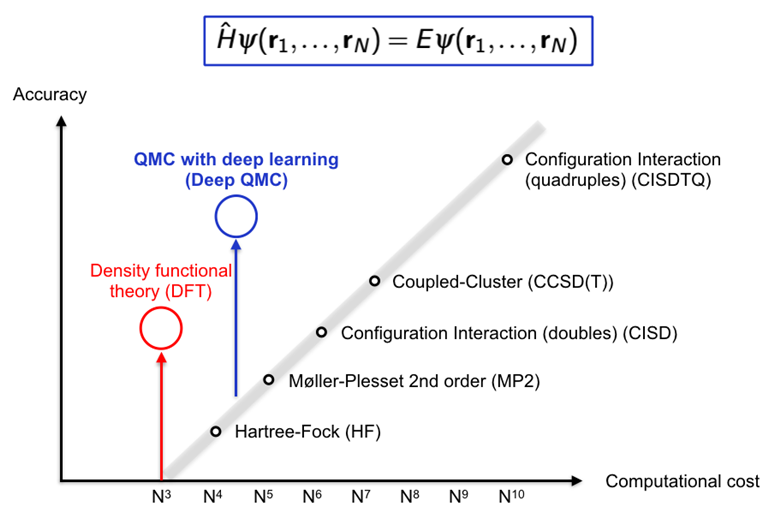
\includegraphics[width=0.9\linewidth]{fig/qm_scaling.png}
    \caption{แผนภาพแสดง Scaling ของวิธีทางเคมีควอนตัม (เครดิตภาพ: https://www.chemistryworld.com)}
    \label{fig:qm_scaling}
\end{figure}

\begin{table}[H]
    \centering
    \caption{ตารางเปรียบเทียบความซับซ้อนเชิงคำนวณของวิธีทางเคมีควอนตัม\autocite{rupp2015} โดย $N$ คือจำนวนของอิเล็กตรอนหรือ%
    จำนวนของ Basis function}
    \label{tab:qm_complx}
    \small
    \begin{tabular}{lll}\toprule
    ตัวย่อ &วิธี &Runtime \\\midrule
    FCI &Full Configuration Interaction (CISDTQ) &$\mathcal{O}(N^{10})$ \\
    CC &Coupled Cluster (CCSDT) &$\mathcal{O}(N^{8})$ \\
    CC &Coupled Cluster (CCSD(T)) &$\mathcal{O}(N^{7})$ \\
    CC &Coupled Cluster (CCSD) &$\mathcal{O}(N^{6})$ \\
    FCI &Full Configuration Interaction (CISD) &$\mathcal{O}(N^{6})$ \\
    MP2 &M$\o$llor-Plesset second order perturbation theory &$\mathcal{O}(N^{5})$ \\
    QMC &Quantum Monte Carlo &$\mathcal{O}(N^{3}) - \mathcal{O}(N^{4})$ \\
    HF &Hartree-Fock &$\mathcal{O}(N^{3}) - \mathcal{O}(N^{4})$ \\
    DFT &Density Functional Theory (Kohn-Sham) &$\mathcal{O}(N^{3})$ \\
    TB &Tight Binding &$\mathcal{O}(N^{3})$ \\
    MM &Molecular Mechanics &$\mathcal{O}(N^{2})$ \\
    \bottomrule
    \end{tabular}
\end{table}

ตารางที่ \ref{tab:qm_complx} แสดงค่าความซับซ้อนของการคำนวณ (Compuational Complexity) ของแต่ละวิธี โดยจะเห็นได้ว่าวิธี DFT 
นั้นมีความซับซ้อนคือ $\mathcal{O}(N^{3})$ นั่นคือมันเป็นสัดส่วนโดยตรงกับจำนวนของอิเล็กตรอนของระบบ ($N$) ยกกำลังสาม ซึ่งมาจาก%
การที่เราจะต้องทำการทำให้ Hamiltonian เกิดเมทริกซ์รูปทแยง (Diagonalization)\footnote{เป็นวิธีการเปลี่ยนฐานของปริภูมิเวกเตอร์%
เพื่อให้ได้เมทริกซ์การแปลงเชิงเส้นที่อยู่ในรูปเมทริกซ์ทแยง เพื่อที่จะนำไปคำนวณในขั้นตอนต่อไปได้อย่างสะดวกมากขึ้น} ซึ่งความซับซ้อนของการทำ 
Diagonalization สำหรับเมทริกซ์จตุรัสขนาด $n \times n$ คือ 
$\mathcal{O}(n^{3})$

\begin{adjustwidth}{-2.5 cm}{-2.5 cm}
    \centering
    \begin{threeparttable}[H]
    \caption{ตารางเปรียบเทียบความซับซ้อนเชิงคำนวณของวิธีทางเคมีควอนตัม\autocite{zotero-328} โดย $n$ คือจำนวนของข้อมูล, $p$ 
    คือจำนวน Feature, $n_{trees}$ คือจำนวนของต้นไม้ (Trees), $n_{sv}$ คือจำนวนของ Support Vectors, $n_{L_{i}}$ 
    คือจำนวนของ Neuron หรือ Node ของชั้นที่ $i$ และ $t$ คือจำนวนของ Epochs ที่ใช้ในการฝึกฝนโมเดล}
    \label{tab:ml_complx}
    \small
    \begin{tabular}{lll}\toprule
    \multirow{2}{*}{อัลกอริทึม} &\multicolumn{2}{c}{Runtime} \\\cmidrule{2-3}
    &การฝึกฝนโมเดล &การทำนายเอาต์พุต\\\midrule
    Decision Tree &$\mathcal{O}(n^{2}p)$ &$\mathcal{O}(p)$ \\
    Random Forest &$\mathcal{O}(n^{2}pn_{trees})$ &$\mathcal{O}(pn_{trees})$ \\
    Gradient Boosting ($n\_{trees}$) &$\mathcal{O}(npn_{trees})$ &$\mathcal{O}(pn_{trees})$ \\
    Linear Regression &$\mathcal{O}(p^{2}n+p^{3})$ &$\mathcal{O}(p)$ \\
    SVM (Kernel) &$\mathcal{O}(n^{2}p+n^{3})$ &$\mathcal{O}(n_{sv}p)$ \\
    Neural Network &$\mathcal{O}(npt*(n_{L_{1}}n_{L_{2}}+ n_{L_{2}}n_{L_{3}} + \dots)$ &$\mathcal{O}(pn_{L_{1}} 
    + n_{L_{1}}n_{L_{2}}+ \dots)$ \\
    \bottomrule
    \end{tabular}
\end{threeparttable}
\end{adjustwidth}

ตารางที่ \ref{tab:ml_complx} แสดงค่าความซับซ้อนของการคำนวณของอัลกอริทึม ML แบบต่าง ๆ เช่นเดียวกับตารางก่อนหน้านี้ 
โดยอัลกอริทึมที่แสดงนั้นถูกใช้กับโจทย์ปัญหา Classification และ Regression (ยกเว้น Linear Regression ที่ใช้สำหรับ Regression 
เท่านั้น) จะเห็นได้ว่าความซับซ้อนของวิธี ML นั้นจะขึ้นอยู่กับจำนวนของข้อมูลและจำนวน Feature ของข้อมูลแต่ละตัวเป็นหลัก ยกเว้นกรณีของ%
โมเดล Neural Network ซึ่งเราสนใจเฉพาะการเรียนรู้เชิงลึก (Deep Learning) เท่านั้นที่ความซับซ้อนของโมเดลจะขึ้นอยู่กับจำนวนรอบที่ใช้%
ในการฝึกสอนโมเดลและจำนวนชั้นของโครงข่าย

ถ้าหากเปรียบเทียบแล้วจะพบว่าวิธี ML นั้นมีความซับซ้อนน้อยกว่าวิธี QM อย่างมีนัยสำคัญ อย่างน้อย ๆ ก็ในระดับหลายเท่าตัว และยิ่งไปกว่านั้น
ความซับซ้อนเชิงการคำนวณในการทำนายค่าเอาต์พุตของโมเดลที่ผ่านการฝึกสอนมาแล้วนั้นต่ำมาก ซึ่งโดยส่วนใหญ่แล้วจะอยู่ในรูปของผลคูณ%
เชิงเส้นแบบดีกรี 1 ระหว่างจำนวนของข้อมูลกับจำนวนของ Feature นี่จึงเป็นเหตุผลที่ทำให้งานวิจัยทางด้านเคมี โดยเฉพาะด้าน QM ในช่วงระยะเวลา
10 ปีที่ผ่านมานั้น นักวิจัยเริ่มให้ความสนใจในการประยุกต์ใช้ ML เพื่อมาใช้ในการสร้างโมเดลสำหรับประมาณค่าหรือทำนายค่าต่าง ๆ ทางควอนตัม 
นั่นก็เพราะ ML เป็นวิธีที่สิ้นเปลืองน้อยกว่า

%--------------------------
\section{ทักษะที่จำเป็นสำหรับผู้เริ่มต้นศึกษาการเรียนรู้ของเครื่อง}
\label{sec:skills_for_ml}
%--------------------------

การมีความรู้พื้นฐานก่อนเริ่มศึกษา ML อย่างจริงจังนั้นมันเป็นสิ่งสำคัญ ผู้เขียนได้สรุป 5 สิ่งสำคัญที่ผู้ที่เริ่มต้นศึกษาควรจะต้องรู้ ดังต่อไปนี้

\begin{enumerate}
    \item \textbf{พีชคณิตเชิงเส้นและแคลคูลัสแบบหลายตัวแปร} : ทั้งสองวิชานี้ถือว่าเป็นรากฐานของ ML เลยก็ว่าได้ 
    เพราะว่าโมเดลทุกรูปแบบของ ML นั้นต่างก็ล้วนแต่เป็นคณิตศาสตร์ ถ้าหากเราต้องการที่จะพัฒนาอัลกอริทึมใหม่ ๆ 
    หรือปรับปรุงอัลกอริทึมที่มีอยู่แล้ว เราจะต้องอาศัยความรู้พีชคณิตเชิงเส้น (เวกเตอร์และเมทริกซ์) และแคลคูลัส (การหาอนุพันธ์) 
    แต่ถ้าหากว่าเราเน้นไปทางสายแอพพลิเคชัน เราก็อาจจะไม่จำเป็นต้องรู้แบบลึกหรือละเอียดมากก็ได้ เพราะว่าในปัจจุบันมีเครื่องมือและไลบรารี่%
    สำเร็จรูปให้เราเลือกใช้มากมาย
    
    \item \textbf{สถิติ} : เนื่องจากว่าในขั้นตอนก่อนที่จะเริ่มสร้างและเทรนโมเดล ML นั้น เราจะต้องใช้เวลาส่วนใหญ่ 
    (อาจจะมากถึง 80\%) ไปกับการรวบรวมข้อมูล ทำความสะอาดข้อมูล การศึกษาการกระจายตัวของข้อมูล การตั้งและทดสอบสมมติฐาน 
    การทำการถดถอย (Regression) การแยกประเภท (Classification) เราจึงจำเป็นจะต้องใช้สถิติเข้ามาช่วยเพื่อให้เข้าใจถึงรายละเอียด
    ของชุดข้อมูลที่เรากำลังจะเล่นกับมัน ยิ่งเข้าใจข้อมูลมากเท่าไหร่ ยิ่งช่วยให้เราสามารถเลือกใช้โมเดล ML ได้เหมาะสมเท่านั้น 
    
    \item \textbf{โปรแกรมมิ่ง} : สิ่งสำคัญลำดับถัดมาคือทักษะในการเขียนโปรแกรมหรือเขียนโค้ด ถึงแม้ว่าเราจะมีความรู้ด้านทฤษฎีที่แม่นยำ 
    แต่ถ้าหากเราไม่สามารถเขียนโปรแกรมได้ แล้วก็ไม่สามารถสร้างโมเดลหรือนำ ML มาใช้งานจริงได้เลย ดังนั้นเราควรจะต้องเรียนรู้การเขียนโปรแกรม
    ให้ได้อย่างน้อยสัก 1 ภาษา ซึ่งภาษาที่ได้รับความนิยมมากที่สุดสำหรับงานทางด้านวิทยาศาสตร์ข้อมูล ณ ตอนนี้คือภาษา Python 
    นั่นก็เพราะตัวภาษาเองมีไวยากรณ์ (Syntax) ที่เข้าใจง่าย มีไลบรารี่ให้เลือกใช้เยอะ มี Community ที่ใหญ่มาก ไม่ต้องกลัวเลยว่าถ้าหากมี%
    ปัญหาเกี่ยวกับการเขียน Python แล้วจะไม่มีคนช่วยหรือหาวิธีแก้ปัญหาไม่ได้ เว็บไซต์ที่มีการถามตอบคำถามเกี่ยวกับการเขียนโปรแกรมที่ได้รับ%
    ความนิยมเป็นอันดับหนึ่งก็คือ Stack Overflow (\url{https://stackoverflow.com/})
    
    \item \textbf{แนวคิดของ ML} : แนวคิดหรือ Concept ทางด้าน ML (วิทยาศาสตร์ข้อมูล) เป็นสิ่งที่สำคัญมากเช่นเดียวกัน
    เราควรจะทราบคำศัพท์เฉพาะทางและความหมาย (Terminology) ประเภทของ ML แนวทางการนำ ML มาใช้ (Best Practice)
    
    \item \textbf{ฝึกทำโจทย์จริง} : ตัวช่วยที่ดีที่สุดให้ทำเราเรียนรู้ ML ได้อย่างรวดเร็วนั่นก็คือการฝึกฝน ทั้งการเขียนโค้ดและการฝึกวิเคราะห์ 
    ลองหาโจทย์จริง ๆ มาฝึกทำ หรืออาจจะลองเก็บเกี่ยวประสบการณ์โดยเข้าร่วมการแข่งขันวิทยาศาสตร์ข้อมูล ซึ่งในปัจจุบันก็มีการจัดแข่งขันบ่อยมาก ๆ 
    เรียกได้ว่ามีสนามให้ได้ฝึกฝนวิทยายุทธเป็นพัน ๆ เลย เช่น Kaggle\footnote{\url{https://www.kaggle.com/competitions}} และ
    AIcrowd\footnote{\url{https://www.aicrowd.com}} 
\end{enumerate}

%--------------------------
\section{แนวทางสำหรับการศึกษาการเรียนรู้ของเครื่อง}
\label{sec:learn_ml}
%--------------------------

ผู้เขียนได้สรุปแนวทางศึกษา ML สำหรับงานวิจัยทางด้านเคมี (เน้นเคมีควอนตัม) สำหรับผู้เริ่มต้นตามด้านล่างต่อไปนี้

\begin{enumerate}
    \item เริ่มจากปรับพื้นฐานพีชคณิตเชิงเส้น (โดยเน้นไปที่เมทริกซ์) และแคลคูลัสแบบหลายตัวแปร เช่น การหาอนุพันธ์ย่อยและเวกเตอร์แคลคูลัส 
    รวมไปถึงวิธีวิเคราะห์ทางสถิติ
    
    \item ดูวิดีโอที่อธิบายปัญญาประดิษฐ์เบื้องต้น เช่น วิดีโอบน YouTube (\url{https://www.youtube.com/watch?v=ukzFI9rgwfU}) 
    หลังจากนั้นให้เรียนคอร์ส ML โดยคอร์สที่ผมแนะนำคือคอร์สออนไลน์ของศาสตราจารย์ Andrew Ng (Stanford University) บน Coursera 
    โดยมีสองคอร์สหลักคือ 
    \begin{enumerate}
        \item Machine Learning Specialization เป็นคอร์ส ML ที่ได้รับความนิยมมากที่สุดในโลก%
        \footnote{\url{https://www.coursera.org/specializations/machine-learning-introduction}}
        \item Deep Learning Specialization เป็นคอร์สที่ได้รับความนิยมไม่แพ้กัน โดยจะเน้นไปที่ Neural Network%
        \footnote{\url{https://www.coursera.org/specializations/deep-learning}}
    \end{enumerate}
    
    \item ทำแบบฝึกหัดตามหนังสือ \enquote{Hands-On Machine Learning with Scikit-Learn, Keras, and TensorFlow: 
    Concepts, Tools, and Techniques to Build Intelligent Systems} และหนังสือ \enquote{Python Machine Learning} 
    เพื่อจะได้ทำความคุ้นเคยกับ Framework ในการเขียนโค้ด ML และ Neural Network
    
    \item ศึกษาการประยุกต์ ML และ Neural Network สำหรับเคมีด้วยเว็บไซต์ \url{https://dmol.pub} ที่จัดทำโดยกลุ่มวิจัยของ%
    ศาสตราจารย์ Andrew White (University of Rochester) ซึ่งจะมีโจทย์ทางเคมีและโค้ดให้ฝึกเขียนตาม เช่น การทำนายคุณสมบัติที่%
    สำคัญและการทำนายพลังงานรวมของโมเลกุล
    
    \item ทบทวนงานวิจัย (Literature Review) ในวารสารวิชาการที่อ่านได้ง่าย ไม่ลงรายละเอียดเชิงเทคนิคมากไป เช่น Chemical Reviews 
    ที่เกี่ยวกับ ML สำหรับเคมีทั่วไปและเคมีควอนตัม
    
    \item เลือกอ่านบทความงานวิจัยจากวารสารเฉพาะทางเน้นไปที่เคมีทฤษฎีและการประยุกต์ โดยเลือกหัวข้องานวิจัยเคมีที่เราสนใจและต้องการ%
    นำ ML ไปประยุกต์ใช้กับหัวข้อนั้น ๆ
\end{enumerate}

อย่างไรก็ตาม แนวทางทั้ง 6 ข้อตามด้านบนนั้นเป็นความคิดเห็นส่วนตัวของผู้เขียนซึ่งอ้างอิงตามประสบการณ์จริง นอกจากแหล่งความรู้ที่ผู้เขียนได้%
แนะนำไว้แล้วจริง ๆ ยังมีแหล่งความรู้อื่น ๆ อีกมากมายที่ผู้อ่านสามารถศึกษาตามได้ด้วยตัวเอง

%--------------------------
\section{คำศัพท์เฉพาะทางด้านการเรียนรู้ของเครื่อง}
\label{sec:ml_term}
%--------------------------

\begin{description}[style=nextline]
    \item[Accuracy] ค่าความถูกต้องของการทำนายของโมเดล ส่วนใหญ่เรามักจะรายงานค่าความถูกต้องเป็นเปอร์เซ็นต์
    \idxboth{ค่าความถูกต้อง}{Accuracy}

    \item[Algorithm] วิธีหรือขั้นตอนกระบวนการคิดคำนวณทางคณิตศาสตร์เพื่อให้ได้ผลลัพธ์ออกมา
    \idxboth{อัลกอริทึม}{Algorithm}

    \item[Attribute] ปริมาณที่ได้จากการสังเกตซึ่งบ่งบอกถึงคุณลักษณะของสิ่งที่สนใจ เช่น สี, ขนาด, และความสูง พูดง่าย ๆ คือถ้าเป็น%
    ชุดข้อมูล Attribute ก็คือชื่อของแต่ละคอลัมน์นั่นเอง
    \idxboth{คุณลักษณะ}{Attribute}

    \item[Categorical Variables] ตัวแปรจัดกลุ่ม ไม่มีความต่อเนื่อง เป็นข้อมูลประเภทแบบแยกออกจากกันและไม่ขึ้นต่อค่าอื่น ๆ เช่น 
    เพศ เชื้อชาติ พันธ์สุนัข ชนิดของผลไม้ ชนิดของหมู่ฟังก์ชันในโมเลกุล
    \idxboth{ตัวแปรจัดกลุ่ม}{Categorical Variables}

    \item[Classification] การจำแนกข้อมูลหรือการทำนายค่าที่มีความไม่ต่อเนื่อง เช่น ประเภทของยานพาหนะ ชนิดของผลไม้
    \idxboth{การจำแนก}{Classification}
 
    \item[Clustering] การจัดกลุ่มข้อมูล
    \idxboth{การจัดกลุ่ม}{Clustering}

    \item[Confusion matrix] เมทริกซ์ที่แสดงการประเมินผลลัพธ์ของการทำนาย
    \begin{itemize}
        \item True Positives (TP): ทำนายว่าจริง และสิ่งที่เกิดขึ้นก็จริง
        
        \item True Negatives (TN): ทำนายว่าไม่จริง และสิ่งที่เกิดขึ้นก็ไม่จริง
        
        \item False Positives (FP): ทำนายว่าจริง แต่สิ่งที่เกิดขึ้นคือไม่จริง
        
        \item False Negatives (FN): ทำนายว่าไม่จริง แต่สิ่งที่เกิดขึ้นคือจริง
    \end{itemize}
    \idxen{Confusion matrix}

    \item[Continuous Variables] ตัวแปรต่อเนื่อง เป็นตัวแปรเชิงปริมาณที่มีค่าในช่วงที่กำหนด เช่น น้ำหนัก จำนวนรถ ความยาวพันธะ
    \idxboth{ตัวแปรต่อเนื่อง}{Continuous Variables}

    \item[Convergence] สถานะของโมเดลเมื่อการเปลี่ยนของค่า Loss ระหว่าง Interation มีขนาดน้อยมาก ๆ
    \idxboth{การลู่เข้า}{Convergence}

    \item[Descriptor] วิธีที่ใช้ในการแปลงข้อมูล เช่น ข้อมูลของโครงสร้างโมเลกุล ให้เป็นข้อมูลเวกเตอร์ที่เป็น Feature
    \idxen{Descriptor}

    \item[Dataset หรือ Data Set] ชุดข้อมูลที่มีคุณสมบัติเหมือนกันโดยถูกจัดเป็นชุดให้ถูกต้องตามลักษณะโครงสร้างข้อมูล
    \idxboth{ชุดข้อมูล}{Dataset}

    \item[Epoch] จำนวนครั้งหรือจำนวนรอบที่อัลกอริทึมมองเห็นหรือได้รับชุดข้อมูลทั้งหมดเข้ามาเพื่อทำการเรียนรู้
    \idxen{Epoch}

    \item[Extrapolation] เป็นการทำนายที่อยู่นอกเหนือจากชุดข้อมูลที่ใช้ในการฝึกสอนโมเดล
    \idxen{Extrapolation}

    \item[Feature] คุณลักษณะเฉพาะของสิ่งที่สนใจ โดยเป็นข้อมูลแบบ 1 มิติที่ถูกสร้างโดย Descriptor
    \idxboth{คุณลักษณะเฉพาะ}{Feature}

    \item[Hyperparameter] พารามิเตอร์ขั้นสูงที่กำหนดคุณสมบัติของโมเดล เช่น ความเร็วในการเรียนรู้ ความซับซ้อนของโมเดล
    ซึ่งผู้ใช้งานจะต้องทำการกำหนดพารามิเตอร์เหล่านี้ก่อนทำการสร้างหรือฝึกสอนโมเดล
    \idxboth{ไฮเปอร์พารามิเตอร์}{Hyperparameter}

    item[Input] อินพุตเป็นข้อมูลที่เรานำเข้าหรือป้อนเข้าไปให้กับโปรแกรมคอมพิวเตอร์
    \idxboth{อินพุต}{Input}

    \item[Learning Rate] อัตราเร็วในการเรียนรู้ของโมเดล หรือในทางทฤษฎีคือขนาดของก้าวในการปรับปรุง (Update Step) ในกระบวนการ 
    Optimization โดยการใช้อัลกอริทึม เช่น Gradient Descent
    \idxboth{อัตราเร็วในการเรียนรู้}{Learning rate}

    \item[Loss] ค่าความคลาดเคลื่อนหรือความแตกต่างระหว่างค่าที่ได้จากการทำนาย (Prediction) และค่าอ้างอิง (Ground Truth หรือ 
    Reference) ยิ่ง Loss มีค่าน้อย หมายความว่าโมเดลของเรายิ่งมีประสิทธิภาพสูง โดยค่า Loss จะถูกคำนวณในระหว่างการฝึกสอนโมเดล
    \idxboth{ค่่าความคลาดเคลื่อน}{Loss}

    \item[Model] ชุดคำสั่งหรือโปรแกรมที่ถูกสร้างขึ้นมาโดยมีความสามารถในการคำนวณ ประมวลผลและตัดสินใจ
    \idxboth{แบบจำลอง}{Model}

    \item[Noise] ข้อมูลที่มีความผิดปกติและไม่มีความเกี่ยวข้องกับข้อมูลที่เราสนใจ รวมไปถึงค่าที่เกิดจากการสุ่ม (Randomness)

    \item[Normalization] การทำให้เป็นปกติ เป็นการกำหนดหรือบังคับค่าของน้ำหนัก (Weights) ในการทำ Regression เพื่อป้องกันปัญหา
    Overfitting (การ Fit ข้อมูลที่ดีเกินไป) และเพิ่มความเร็วในการคำนวณ
    \idxboth{การทำให้เป็นปกติ}{Normalization}

    \item[Outlier] ค่าที่ผิดปกติไปจากข้อมูลตัวอื่นในชุดข้อมูล
    \idxen{Outlier}

    \item[Output] เอาต์พุตเป็นข้อมูลที่ถูกส่งออกมาจากโปรแกรมคอมพิวเตอร์
    \idxboth{เอาต์พุต}{Output}

    \item[Overfitting] คือการที่โมเดลที่ถูกฝึกสอนด้วยชุดข้อมูล Training Set มีค่าความถูกต้องในการบ่งบอกคลาสเป้าหมายสูง 
    แต่เมื่อนำไปใช้กับข้อมูลทดสอบ Test Set กลับได้ค่าความถูกต้องต่ำ กล่าวอีกนัยหนึ่งคือตัวโมเดลที่ได้สามารถเรียนรู้ข้อมูลจาก Training Set 
    ได้ดีมาก แต่ไม่สามารถนำไปใช้กับข้อมูลใหม่ที่ไม่เคยพบมาก่อน (Unknown Data) ได้ดี
    \idxen{Overfitting}

    \item[Parameter] คุณสมบัติของข้อมูลที่ถูกเรียนรู้โดยโมเดลปัญญาประดิษฐ์ โดยพารามิเตอร์จะถูกปรับให้มีความเหมาะสมตามอัลกอริทึมที่ใช้
    เช่น Optimization ตัวอย่างของพารามิเตอร์มีดังนี้
    \begin{itemize}
        \item น้ำหนัก (Wegiths) ในเทคนิค Neural Network
        
        \item Support Vectors ในเทคนิค Support Vector Machine
        
        \item ค่าสัมประสิทธิ์ (Coefficients) ในเทคนิค Linear Regression
    \end{itemize}
    \idxboth{พารามิเตอร์}{Parameter}

    \item[Precision] ความแม่นยำของการทำนาย มีสมการในการคำนวณดังนี้
    \begin{equation}\label{eq:precision}
        P = \frac{\text{True Positives}}{\text{True Positives} + \text{False Positives}}
    \end{equation}

    \item[Prediction] กระบวนการทำนายค่าของโมเดลโดยจะทำนายค่าเอาต์พุตของข้อมูลใหม่ที่ถูกป้อนเข้าไป
    \idxboth{การทำนาย}{Prediction}

    \item[Regression]  การทำนายค่าที่มีความต่อเนื่อง เช่น ราคาสินค้า ปริมาณน้ำมัน ถ้าในบริบทของเคมีก็จะเป็นคุณสมบัติของโมเลกุล 
    เช่น พลังงานภายในของโมเลกุล, พลังงานอิสระของโมเลกุล และพลังงานกระตุ้น
    \idxen{Regression}

    \item[Regularization] การทำให้ถูกต้อง เป็นเทคนิคสำหรับการแก้ปัญหา Overfitting โดยการเพิ่มพจน์พิเศษที่มีความซับซ้อนเข้าไปใน 
    Loss function โดยเทคนิคนี้มีประโยชน์อย่างมากในการสร้างโมเดลที่มีความซับซ้อน
    \idxboth{การทำให้ถูกต้อง}{Regularization}

    \item[Reinforment Learning] การเรียนรู้แบบเสริมแรง 
    \idxboth{การเรียนรู้แบบเสริมแรง}{Reinforment Learning}

    \item[Representation] Feature ของโมเลกุลในรูปแบบสัญลักษณ์ (Symbolic) เช่น SMILES, InChI, สูตรโมเลกุล
    \idxen{Representation}

    \item[Segmentation] กระบวนการหรือขั้นตอนการแบ่งส่วนของชุดข้อมูลออกเป็นหลาย ๆ ชุดข้อมูลย่อย
    \idxen{Segmentation}

    \item[Specificity] ความจำเพาะเจาะจง เป็นพารามิเตอร์ที่วัเประสิทธิภาพของโมเดลในการจำแนกกรณีที่เป็นเท็จหรือไม่เป็นจริง (Negative)
    กล่าวอีกอย่างคือ เมื่อคำตอบคือ Negative พารามิเตอร์ตัวนี้จะบอกเราว่าการทำนายของโมเดลของเรานั้นถูกต้องมากน้อย (บ่อย) แค่ไหน
    โดยมีสมการที่ในการคำนวณคือ
    \begin{equation}\label{eq:specficity}
        S = \frac{\text{True Negatives}}{\text{True Negatives} + \text{False Positives}}
    \end{equation}
    \idxboth{ความจำเพาะเจาะจง}{Specificity}

    \item[Supervised Learning] การเรียนรู้ของโมเดลแบบมีผู้สอน (Output)
    \idxboth{การเรียนรู้แบบมีผู้สอน}{Supervised Learning}

    \item[Target / Output / Class / Label] คำตอบหรือเป้าหมายที่ต้องการคำนวณ (Calculate) ประมาณค่า (Approximate) 
    หรือทำนาย (Predict)
    \idxen{Target}
    \idxen{Output}
    \idxen{Class}
    \idxen{Label}

    \item[Test Set] ชุดข้อมูลที่ใช้ทดสอบความถูกต้องและแม่นยำของ Model
    \idxboth{ชุดข้อมูล!ชุดข้อมูลสำหรับการทดสอบ}{Test Set}

    \item[Training] กระบวนการสร้างและฝึกสอนโมเดลโดยใช้ Training set 
    \idxboth{การฝึกสอน}{Training}

    \item[Training Set] ชุดข้อมูลที่นำมาใช้ในการสอนคอมพิวเตอร์เพื่อสร้าง Model
    \idxboth{ชุดข้อมูล!ชุดข้อมูลสำหรับการฝึกสอน}{Training Set}

    \item[Transfer Learning] การเรียนรู้แบบส่งต่อ เป็นการนำโมเดล ML ที่ผ่านการฝึกสอนแล้วและสามารถทำงานอย่างหนึ่งได้อยู่แล้วมา%
    ฝึกสอนอีกครั้งหนึ่งเพื่อให้สามารถทำงานที่สองได้ โดยวิธีการทำ Transfer Learning ก็คือเรานำค่าพารามิเตอร์ที่ถูกปรับโดยผ่านการฝึกสอนแล้ว
    นำมาใช้ต่อในการทำนายค่าอื่น ๆ นั่นเอง ตัวอย่างเช่นถ้าเป็น Neural Network พารามิเตอร์ที่เรามาสามารถนำมาใช้ได้ก็จะเป็นน้ำหนัก (Weights) 
    ของแต่ละ Layer เป็นต้น
    \idxboth{การเรียนรู้แบบส่งต่อ}{Transfer Learning}

    \item[Unsupervised Learning] การเรียนรู้ของโมเดลแบบไม่มีผู้สอน (Output-free)
    ซึ่งยังสามารถแบ่งออกได้เป็นสองประเภทคือ 1. Binary Classification กับ 2. Multi-class Classification
    \idxboth{การเรียนรู้แบบมีไม่มีผู้สอน}{Unsupervised Learning}

    \item[Validation Set] ชุดข้อมูลสำหรับประเมินประสิทธิภาพของโมเดลก่อนที่จะนำไปทดสอบกับ Test Set จริง 
    โดย Dataset ประเภทนี้มักจะถูกนำมาใช้ในการทำ Cross-validation
    \idxboth{ชุดข้อมูล!ชุดข้อมูลสำหรับการประเมินผล}{Validation Set}
\end{description}
 % การเรียนรู้ของเครื่อง
% LaTeX source for ``การเรียนรู้ของเครื่องสำหรับเคมีควอนตัม (Machine Learning for Quantum Chemistry)''
% Copyright (c) 2022 รังสิมันต์ เกษแก้ว (Rangsiman Ketkaew).

% License: Creative Commons Attribution-NonCommercial-NoDerivatives 4.0 International (CC BY-NC-ND 4.0)
% https://creativecommons.org/licenses/by-nc-nd/4.0/

\chapter{การเรียนรู้แบบมีผู้สอน}
\label{ch:sup_ml}

\begin{figure}[H]
    \centering
    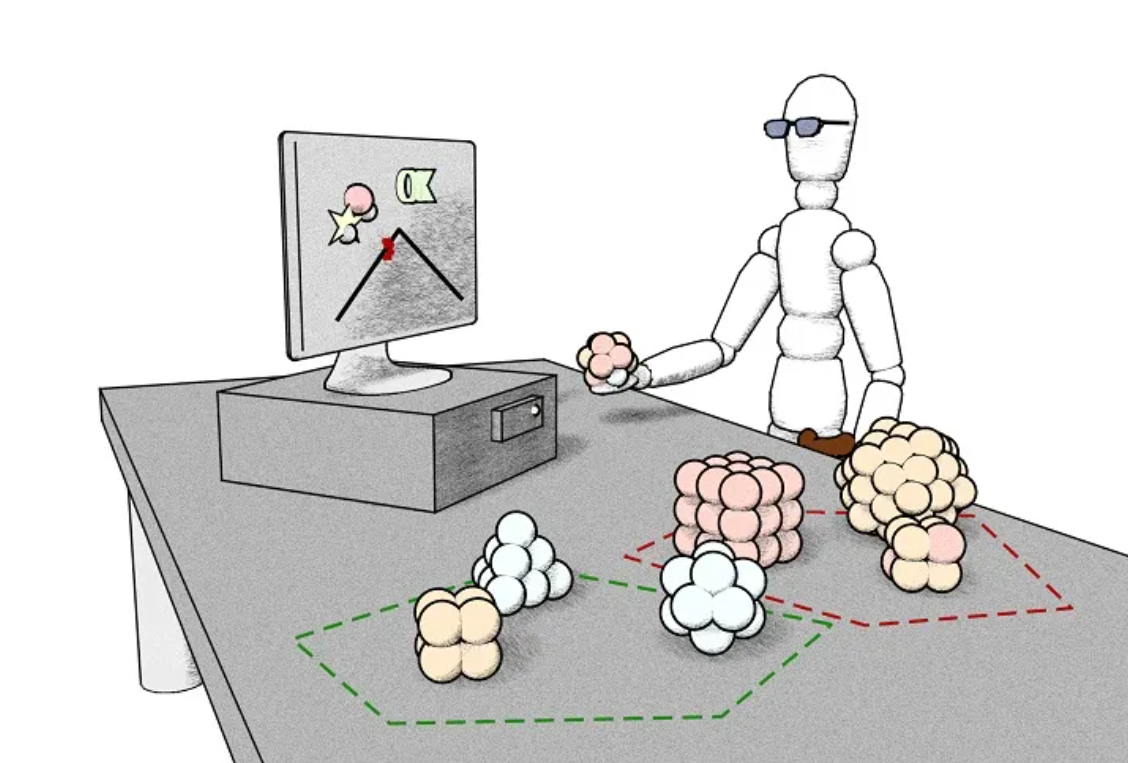
\includegraphics[width=0.65\linewidth]{fig/supervised_ml.png}
    \caption{หุ่นยนต์กำลังเรียนรู้หาความเชื่อมโยงระหว่างโครงสร้างกับคุณสมบัติของโมเลกุล (เครดิตภาพ: https://puentesdigitales.com)}
    \label{fig:supervised_ml}
\end{figure}

การเรียนรู้แบบมีผู้สอนหรือ Supervised Learning เป็นเทคนิคแรก ๆ ที่ถูกพัฒนาขึ้นมาในช่วงยุคเริ่มต้นของ ML ซึ่งเป็นแนวคิดที่ใช้อินพุตและเอาต์พุตในการฝึกสอนโมเดล ซึ่งโมเดลที่ได้ออกมานั้นจะเก็บข้อมูลที่อธิบายความสัมพันธ์ระหว่างอินพุตและเอาต์พุตนั่นเอง $($เปรียบเสมือนฟังก์ชันทางคณิคศาสตร์ $f(x))$ ซึ่งผู้เขียนมีความคิดเห็นส่วนตัวว่าการสร้างโมเดลประเภทนี้ง่ายกว่าประเภทอื่นทั้งในแง่ทฤษฎีของอัลกอริทึม การเรียนรู้ของผู้เริ่มต้นศึกษาและการนำไปใช้จริง โดยเทคนิคนี้ได้รับความนิยมมากที่สุดนั่นก็เพราะว่าสามารถนำไปประยุกต์ใช้งานกับโจทย์ที่หลากหลาย

Supervised ML เป็นเทคนิคที่เข้าใจได้ง่ายที่สุดเพราะว่าเป็นการฝึกให้โมเดลมีความสามารถในการเรียนรู้ Target อย่างตรงไปตรงมา จริง ๆ แล้วนิยามของ Supervised ML นั้นมีเยอะมากขึ้นอยู่กับว่าเราต้องการนิยามในเชิงปรัชญา เชิงคณิตศาสตร์ หรือเชิงปฏิบัติ ทุกครั้งที่มีคนถามผู้เขียนว่า Supervised ML คืออะไร ผู้เขียนก็มักจะตอบไปสั้น ๆ แบบไม่จริงจังว่า \enquote{\textit{Supervised ML คือการ Fit Curve}} (จริง ๆ แล้ว ML ทุกอัลกอริทึมเลยก็ว่าได้) ซึ่งการให้นิยามแบบนี้เป็นการอธิบายในเชิงปฏิบัติ ตัวอย่างเช่น กำหนดให้มีข้อมูลในตารางที่ \ref{tab:simple_x_y} เป็นความสัมพันธ์ระหว่างโดเมน (Domain) และเรนจ์ (Range) ของฟังก์ชันเลขชี้กำลังง่าย ๆ ดังต่อไปนี้

\begin{table}[H]
    \centering
    \caption{ตัวอย่างข้อมูลอินพุตกับเอาต์พุตของฟังก์ชันเลขชี้กำลัง (Exponential Function)}
    \label{tab:simple_x_y}
    \begin{tabular}{cc}
        \toprule
        \textbf{Input $(x)$} & \textbf{Output $(y)$} \\
        \midrule
        1                    & 5                     \\
        2                    & 25                    \\
        3                    & 125                   \\
        4                    & 625                   \\
        5                    & ?                     \\
        \bottomrule
    \end{tabular}
\end{table}

ถ้าหากถามว่ากรณีที่อินพุต $(x)$ เท่ากับ 5 แล้วเอาต์พุต $(y)$ มีค่าเท่ากับเท่าไร ผู้อ่านก็คงตอบได้ทันทีเลยว่าเท่ากับ 3125 เพราะว่ามนุษย์นั้นมองเห็นรูปแบบที่เกิดขึ้นระหว่าง $x$ กับ $y$ ซึ่งการเปลี่ยนของ $y$ นั้นก็คือเพิ่มขึ้นครั้งละ 5 เท่า โดยสัมพันธ์กับการเปลี่ยนแปลงของ $x$ ที่เพิ่มขึ้นครั้งละ 1 ดังนั้นจากกรณีที่ $x$ เปลี่ยนจาก 4 เป็น 5 ค่าของ $y$ นั้นก็จะต้องเพิ่มขึ้นจาก 625 เป็น 625 $\times$ 5 = 3125 นั่นเอง สำหรับความสัมพันธ์นี้เราสามารถสรุปฟังก์ชันคณิตศาสตร์ได้เป็น $y = 5^{x}$

ประเด็นที่น่าสนใจก็คือถ้าหากเราถามคำถามเดียวกันนี้กับคอมพิวเตอร์หรือเครื่องจักรว่าคำตอบของ $y$ จะมีค่าเป็นเท่าไรเมื่อ $x = 5$ แน่นอนว่าการรับรู้ของเครื่องจักรนั้นไม่สามารถเทียบเท่ากับการรับรู้ของมนุษย์ถึงแม้ว่าเครื่องจักรจะประมวลผลได้เร็วกว่ามากก็ตาม (ความสามารถในการรับรู้กับความสามารถในการประมวลนั้นต่างกันนะครับ) ดังนั้นสิ่งที่เราต้องการให้เครื่องจักรมีเหมือนมนุษย์ก็คือความสามารถในการเรียนรู้รูปแบบของข้อมูลโดยคำนวณออกมาเป็นฟังก์ชันคณิตศาสตร์ แต่แน่นอนว่าถ้าหากมนุษย์เจอโจทย์หรือข้อมูลที่มีความซับซ้อน เช่น ความสัมพันธ์ที่ไม่เป็นเชิงเส้น ก็ยากที่จะหาคำตอบหรือฟังก์ชันออกมาได้เช่นเดียวกัน ดังนั้นข้อดีของเครื่องจักรก็คือนำความสามารถหรือความเร็วในการคำนวณมาใช้ในการปรับปรุงความสามารถในการเรียนรู้หรือที่เราเรียกว่าการฝึกสอนหรือเทรน (Train) โมเดลนั่นเอง
\idxboth{การฝึกสอนโมเดล}{Model Training}

%--------------------------
\section{การถดถอยเชิงเส้น}
\label{sec:lin_res}
\idxth{การเรียนรู้แบบมีผู้สอน!การถดถอยแบบเชิงเส้น}
\idxen{Supervised Learning!Linear Regression}
%--------------------------

เทคนิคของการเรียนรู้แบบมีผู้สอนที่พื้นฐานที่สุดและได้รับความนิยมอย่างมากในช่วงยุคแรกของปัญญาประดิษฐ์ก็คือ การถดถอยแบบเชิงเส้น (Linear Regression) สมมติว่าเราพิจารณาชุดข้อมูลที่มีตัวแปรต้น 2 ตัว $(x_{1}$ และ $x_{2})$ และมีตัวแปรตาม 1 ตัว $(y)$ ซึ่งตัวแปรตามในที่นี้ก็คือคำตอบหรือเป้าหมายที่เราต้องการทำนายนั่นเอง โดยยกตัวอย่างเช่น กำหนดให้ $x_{1}$ เป็นจำนวนพันธะเดี่ยวในโมเลกุล $x_{2}$ เป็นจำนวนวงอะโรมาติก (Aromatic) ในโมเลกุล และ $y$ เป็นค่าพลังงานรวมของโมเลกุล เราพบว่าเราสามารถสร้างหรือกำหนดสมการที่อธิบายความสัมพันธ์ระหว่างตัวแปรทั้งสามตัวนี้ได้แบบง่าย ๆ ดังนี้
%
\begin{equation}
    h_\theta(x) = \theta_0 + \theta_1 x_1 + \theta_2 x_2
\end{equation}
%
\noindent โดยที่ $x$ ในที่นี้คือเวกเตอร์แบบสองมิติในปริภูมิ $\mathbb{R}^{2}$ และ $\theta_{i}$ คือพารามิเตอร์หรือเรียกว่าน้ำหนัก (Weights) ก็ได้ ซึ่งจะเป็นตัวแปรที่ปรับความเชื่อมโยง (Mapping) ระหว่าง $x_{i}$ และ $y$ ซึ่งเราสามารถเขียนให้อยู่ในรูปทั่วไปได้ดังนี้
%
\begin{align}
    h(x) & = \sum_{i=0}^{d} \theta_{i} x_{i} \\
         & = \theta^{\top} x
\end{align}
%
\noindent โดยสมการด้านบนนั้นจะเขียนในรูปของผลคูณระหว่างเวกเตอร์ของพารามิเตอร์ $(\theta^{\top})$ และเวกเตอร์ $x$

ลำดับถัดมาคือเราจะทำการปรับพารามิเตอร์ $\theta$ อย่างไรเพื่อให้ได้ชุดพารามิเตอร์ที่ทำการ Mapping ได้ดีที่สุด คำตอบก็คือเราสามารถทำได้โดยการกำหนดฟังก์ชันที่จะเป็นตัววัดพารามิเตอร์ $\theta_{i}$ ทีละตัว ซึ่งเรากำหนดและเรียกฟังก์ชันที่จะมาช่วยเราว่า Cost Function (Loss Function) โดยมีรูปสมการทั่วไปดังต่อไปนี้
%
\begin{equation}
    J(\theta) = \frac 1 2 \sum_{i=1}^n \left( h_\theta(x^{(i)}) - y^{(i)} \right)^2
\end{equation}

\noindent ซึ่งจะมีความคล้ายกันกับ Ordinary Least Square นั่นเอง โดยในหัวข้อต่อไปเราจะมาดูรายละเอียดของเทคนิคที่เราสามารถนำมาใช้ในการแก้ปัญหาของ Cost Function

ขออธิบายเสริมครับ: สำหรับฟังก์ชันที่มีความเป็นเชิงเส้นนั้นจะต้องสอดคล้องกับเงื่อนไขดังต่อไปนี้
%
\begin{equation}
    f(\vec{x} + \vec{y}) = f(\vec{x}) + f(\vec{y})
\end{equation}
%
\noindent สำหรับ $\vec{x}$ และ $\vec{y}$ ทุกค่า และเงื่อนไขที่สองคือ
%
\begin{equation}
    f(s\vec{x}) = sf(x)
\end{equation}
%
ถ้าหากฟังก์ชันไม่สอดคล้องกับเงื่อนไขทั้งสองข้อด้านบน ฟังก์ชันนั้นจะมีความไม่เป็นเชิงเส้น (Nonlinearity)

%--------------------------
\subsection{การถดถอยแบบง่าย}
\label{ssec:simple_lin_res}
\idxth{การเรียนรู้แบบมีผู้สอน!การถดถอยแบบง่าย}
\idxen{Supervised Learning!Simple Regression}
%--------------------------

เรามาดูตัวอย่างของกรณีแรกของการถดถอย นั่นก็คือการถดถอยแบบง่าย (Simple Regression) โดยพิจารณาข้อมูลในตาราง
\ref{tab:simple_reg_data} ดังต่อไปนี้
%
\begin{table}[H]
    \centering
    \caption{แสดงเงินที่ใช้ในการลงทุนการโฆษณาของบริษัทต่าง ๆ กับยอดขายรายปี}
    \label{tab:simple_reg_data}
    \begin{tabular}{lcc}
        \toprule
        \textbf{บริษัท} & \textbf{วิทยุ} & \textbf{ยอดขาย (ต่อหน่วย)} \\
        \midrule
        Amazon        & 37.8         & 22.1                     \\
        Google        & 39.3         & 10.4                     \\
        Facebook      & 45.9         & 18.3                     \\
        Apple         & 41.3         & 18.5                     \\
        \bottomrule
    \end{tabular}
\end{table}
%
ตารางที่ \ref{tab:simple_reg_data} แสดงความสัมพันธ์ระหว่างเงินที่ใช้ในการลงทุนในสื่อวิทยุของบริษัทต่าง ๆ กับยอดขายรายปีต่อหน่วยการลงทุน โดยเราสามารถกำหนดตัวแปรได้เป็นตัวแปร $x$ กับ $y$ ซึ่งเป็นอินพุตและเอาต์พุตตามลำดับ ดังสมการต่อไปนี้
%
\begin{equation}
    y = mx + b
\end{equation}
%
\noindent โดยที่ $m$ คือความชันหรือน้ำหนัก (Weight) และ $b$ คือจุดตัดแกน $y$ หรือความโน้มเอียง (Bias) นั่นเอง สำหรับ Loss
Function ที่เราจะเลือกใช้นั้น คือ Mean Square Error (MSE)
%
\begin{equation}
    \text{MSE} = \frac{1}{N} \sum_{i=1}^{n} (y_i - (m x_i + b))^2
\end{equation}
%
ในการ Optimize ฟังก์ชัน MSE ด้านบนนั้นเราจะใช้เทคนิค Gradient Descent ซึ่งเป็นเทคนิคที่เราจะคำนวณหา Gradient ซึ่งสามารถใช้สมการที่
\eqref{eq:grad_simple_reg} ในการคำนวณได้
%
\begin{align}\label{eq:grad_simple_reg}
    f'(m,b) & =
    \begin{bmatrix}
        \dv{f}{m} \\
        \dv{f}{b} \\
    \end{bmatrix}                                  \\
            & =
    \begin{bmatrix}
        \frac{1}{N} \sum -x_i \cdot 2(y_i - (mx_i + b)) \\
        \frac{1}{N} \sum -1 \cdot 2(y_i - (mx_i + b))   \\
    \end{bmatrix} \\
            & =
    \begin{bmatrix}
        \frac{1}{N} \sum -2x_i(y_i - (mx_i + b)) \\
        \frac{1}{N} \sum -2(y_i - (mx_i + b))    \\
    \end{bmatrix}
\end{align}

หลังจากนั้นเราจะทำการฝึกสอนโมเดลโดยการใช้วิธีวนซ้ำเพื่อปรับค่าพารามิเตอร์ต่าง ๆ ทั้ง Weight และ Bias โดยภาพด้านล่างแสดงการเปลี่ยนแปลงของการทาบเส้นตรงกับข้อมูล (Fitting) ระหว่างการฝึกสอน เราจะพบว่าเส้นตรง (Linear Line) ของเรานั้นจะลากผ่านข้อมูลที่อยู่ในช่วงบริเวณตรงกลางได้ดีขึ้นเรื่อย ๆ

\begin{figure}[H]
    \centering
    \begin{subfigure}{0.5\textwidth}
        \centering
        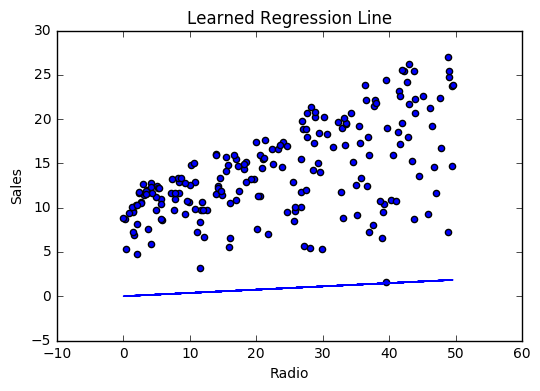
\includegraphics[width=\linewidth]{fig/plot_simple_reg_1.png}
        \caption{ครั้งที่ 1}
        \label{fig:plot_simple_reg_1}
    \end{subfigure}%
    \begin{subfigure}{0.5\textwidth}
        \centering
        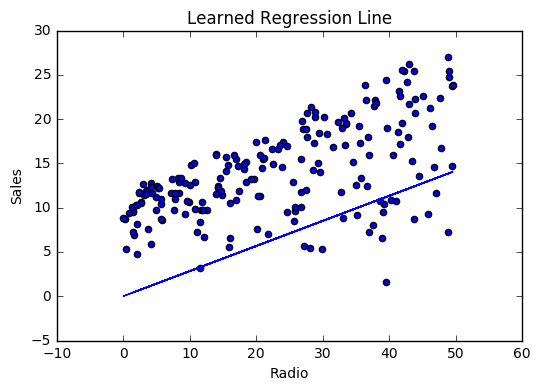
\includegraphics[width=\linewidth]{fig/plot_simple_reg_2.png}
        \caption{ครั้งที่ 2}
        \label{fig:plot_simple_reg_2}
    \end{subfigure}
    \\
    \begin{subfigure}{0.5\textwidth}
        \centering
        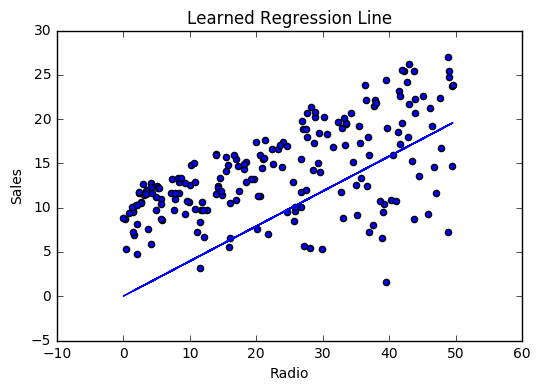
\includegraphics[width=\linewidth]{fig/plot_simple_reg_3.png}
        \caption{ครั้งที่ 3}
        \label{fig:plot_simple_reg_3}
    \end{subfigure}%
    \begin{subfigure}{0.5\textwidth}
        \centering
        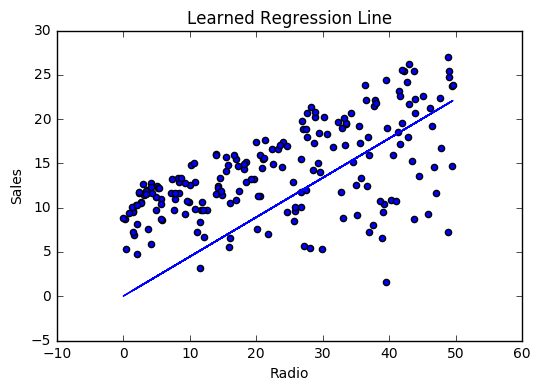
\includegraphics[width=\linewidth]{fig/plot_simple_reg_4.png}
        \caption{ครั้งที่ 4}
        \label{fig:plot_simple_reg_4}
    \end{subfigure}
    \caption{การเปลี่ยนแปลงของเส้นตรงที่ถูกทาบ (Fitting) เข้ากับชุดข้อมูลอย่างง่าย}
    \label{fig:simple_reg_change}
\end{figure}

%--------------------------
\subsection{การถดถอยแบบหลายตัวแปร}
\label{ssec:multi_lin_res}
\idxth{การเรียนรู้แบบมีผู้สอน!การถดถอยแบบหลายตัวแปร}
\idxen{Supervised Learning!Multivariate Regression}
%--------------------------

สำหรับกรณีที่เรามีอินพุตหรือ Feature มากกว่าหนึ่งตัว เช่น ข้อมูลในตาราง \ref{tab:multi_reg_data} ด้านล่างที่เป็นการนำข้อมูลในตาราง \ref{tab:simple_reg_data} มาเพิ่มข้อมูลเงินที่ใช้ในการลงทุนสำหรับการโฆษณาทางสื่อโทรทัศน์และหนังสือพิมพ์เข้าไป (คอลัมน์ที่ 3 กับ 4)

\begin{table}[H]
    \centering
    \caption{แสดงเงินที่ใช้ในการลงทุนการโฆษณาของบริษัทต่าง ๆ กับยอดขายรายปี}
    \label{tab:multi_reg_data}
    \begin{tabular}{lcccc}\toprule
        \textbf{บริษัท} & \textbf{วิทยุ} & \textbf{โทรทัศน์} & \textbf{หนังสือพิมพ์} & \textbf{ยอดขาย (ต่อหน่วย)} \\\midrule
        Amazon        & 37.8         & 230.1           & 69.1              & 22.1                     \\
        Google        & 39.3         & 44.5            & 23.1              & 10.4                     \\
        Facebook      & 45.9         & 17.2            & 34.7              & 18.3                     \\
        Apple         & 41.3         & 151.5           & 13.2              & 18.5                     \\
        \bottomrule
    \end{tabular}
\end{table}

\begin{figure}[H]
    \centering
    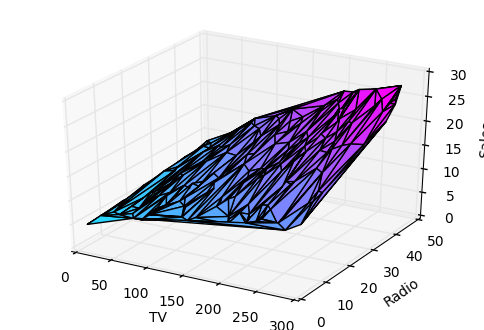
\includegraphics[width=0.6\linewidth]{fig/plot_multivar_reg.png}
    \caption{ความสัมพันธ์ของข้อมูลหลายตัวแปร (Multivariables Data)}
    \label{fig:multi_var_reg}
\end{figure}

โดยในกรณีที่ข้อมูลมีความซับซ้อนมากขึ้นแบบนี้ เราไม่สามารถใช้สมการเส้นตรงแบบง่าย ๆ ที่เราใช้ไปก่อนหน้านี้มาอธิบายความสัมพันธ์ระหว่าง Feature ได้ ดังนั้นเราจะต้องมีการกำหนด Loss Function ขึ้นมาใหม่ โดยตอนนี้เราจะต้องมีการกำหนดค่า Weight ขึ้นมา 3 ค่า นั่นคือจากที่เราเคยมีฟังก์ชัน $mx + b$ ก็จะกลายเป็นฟังก์ชัน $W_1 x_1 + W_2 x_2 + W_3 x_3$ โดยจะได้สมการ Loss Function ใหม่ดังนี้
%
\begin{equation}
    \text{MSE} = \frac{1}{2N} \sum_{i=1}^{n} (y_i - (W_1 x_1 + W_2 x_2 + W_3 x_3))^2
\end{equation}

สำหรับสมการที่เราจะมาใช้ในการหา Gradient ของกรณีนี้สามารถพิสูจน์ได้โดยใช้กฎลูกโซ่ (Chain Rule) เช่นเดียวกับกรณีก่อนหน้านี้
%
\begin{align}
    f'(W_1) = -x_1(y - (W_1 x_1 + W_2 x_2 + W_3 x_3)) \\
    f'(W_2) = -x_2(y - (W_1 x_1 + W_2 x_2 + W_3 x_3)) \\
    f'(W_3) = -x_3(y - (W_1 x_1 + W_2 x_2 + W_3 x_3))
\end{align}

%--------------------------
\section{การจำแนกประเภท}
\label{sec:classification}
\idxth{การเรียนรู้แบบมีผู้สอน!การจำแนกประเภท}
\idxen{Supervised Learning!Classification}
%--------------------------

ในหัวข้อนี้จะเป็นการศึกษาโจทย์ปัญหาแบบการจำแนกประเภท (Classification) ซึ่งก็คล้าย ๆ กับโจทย์แบบ Regression แต่ว่าจะต่างกันตรงที่ค่า $y$ ที่เราต้องการทำนายนั้นจะมีความไม่ต่อเนื่อง (Discrete Data) ซึ่งจะตรงข้ามกับ Regression ที่ค่า $y$ จะมีความต่อเนื่อง (Continuous Data) โดยเริ่มต้นเราจะสนใจกรณี Classification แบบง่ายก่อน นั่นก็คือมีประเภทของข้อมูลที่เราจะจำแนกเพียงแค่ 2 ประเภท เรียกว่าโจทย์ปัญหา Binary Classification ซึ่งค่า $y$ จะมีค่าได้แค่ 0 กับ 1 เท่านั้น ซึ่งในภายหลังเราจึงค่อยมาพิจารณากรณีที่มีประเภทมากกว่า 2 ประเภท (Multiple-class Case)

สำหรับการระบุชื่อของประเภทหรือคลาส (Class) นั้น เราจะเรียกคลาส 0 ว่าเป็น Negative Class และเรียกคลาส 1 ว่า Positive Class ซึ่งบ่อยครั้งเรามักจะเจอการใช้เครื่องหมาย - และ + แทนการเขียน 0 กับ 1 โดยที่เราจะกำหนดให้ $y^{i}$ คือ Label ของข้อมูลลำดับที่ $i$ สำหรับตัวอย่างการฝึกสอน

%--------------------------
\section{การถดถอยแบบโลจิสติค}
\label{sec:logis_regress}
\idxth{การเรียนรู้แบบมีผู้สอน!การถดถอยแบบโลจิสติค}
\idxen{Supervised Learning!Logistic Regression}
%--------------------------

การวิเคราะห์การถดถอยโลจิสติค (Logistic Regression) เป็นการวิเคราะห์ที่มีเป้าหมายเพื่อประมาณค่าหรือทํานายเหตุการณ์ที่สนใจว่าจะเกิดหรือไม่เกิดเหตุการณ์นั้นภายใต้อิทธิพลของตัวปัจจัยโดยอาศัยฟังก์ชันโลจิสติค (Logistic Function) ที่สร้างขึ้นจากชุดตัวแปรทำนายที่เป็นตัวแปรที่มีข้อมูลอยู่ในระดับช่วงเป็นอย่างน้อย โดยที่ระหว่างตัวแปรทำนายจะต้องมีความสัมพันธ์กันต่ำและในการวิเคราะห์จะต้องใช้ขนาดตัวแปรทำนายไม่ต่ำกว่า 30 ตัวแปร Logistic Regression จัดเป็นเครื่องมือวิเคราะห์ข้อมูลในการศึกษาวิจัยที่มีวัตถุประสงค์เพื่อทํานายเหตุการณ์หรือประเมินความเสี่ยง (เช่น \enquote{เสี่ยง} หรือ \enquote{ไม่เสี่ยง}) จึงมีการประยุกต์ใช้ในงานวิจัยหลากหลายสาขา ทั้งสาขาทางการแพทย์ วิศวกรรมศาสตร์ นิเวศวิทยา เศรษฐศาสตร์ และสังคมศาสตร์
\idxboth{การถดถอยโลจิสติค}{Logistic Regression}
\idxboth{ฟังก์ชันโลจิสติค}{Logistic Function}

นอกจากการทำนายการเกิดเหตุการณ์ที่สนใจว่าเกิด (0) หรือไม่เกิด (1) ได้แล้ว Logistic Regression ยังสามารถทำนายค่าความน่าจะเป็นของเหตุการณ์ได้ด้วย (ค่าระหว่าง 0 กับ 1) จริง ๆ แล้วเทคนิค Logistic Regression นั้นคล้ายกับ Linear Regression มาก โดยทั้งสองเทคนิคนี้ต่างกันตรงที่การนำไปใช้งาน โดยเราใช้ Linear Regression สำหรับการแก้ปัญหาการถดถอยแต่ Logistic Regression สำหรับการแก้ปัญหาการแยกคลาสหรือจัดกลุ่มของข้อมูล

\begin{figure}[H]
    \centering
    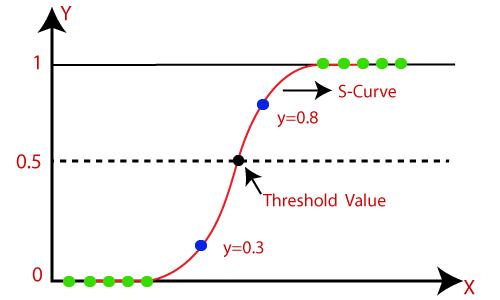
\includegraphics[width=0.6\linewidth]{fig/s_curve_logistic_func.png}
    \caption{Logistic Function หรือ Sigmoid Function}
    \label{fig:s_curve_logistic}
\end{figure}

การทำ Logistic Regression นั้นเราไม่ได้ทำการ Fit เส้น Regression กับข้อมูลแต่จะเป็นการ Fit กับ Logistic Function (ภาพที่ \ref{fig:s_curve_logistic}) แทนซึ่งจะเป็นตัวที่ทำนายค่าออกมา โดย Logistic Function ที่เราใช้นั้นจริง ๆ แล้วก็คือเส้นโค้งตัว S หรือ Sigmoid Function นั่นเอง โดยมีนิยามทางคณิตศาสตร์ดังต่อไปนี้
\idxen{Supervised Learning!Logistic Regression!Sigmoid Function}
%
\begin{equation}\label{eq:logistic_func}
    f(x) = \frac{L}{1 + e^{-k(x-x_0)}}
\end{equation}
%
\noindent สำหรับกรณีที่กำหนดให้ $k = 1$, $x_{0} = 0$, และ $L = 1$ เราจะได้สมการดังต่อไปนี้
%
\begin{align}\label{eq:std_logis_func}
    f(x) & = \frac{1}{1 + e^{-x}} \nonumber                  \\
         & = \frac{e^x}{e^x + 1} \nonumber                   \\
         & = \frac12 + \frac12 \tanh\left(\frac{x}{2}\right)
\end{align}

\noindent ซึ่งเราเรียกสมการที่ \eqref{eq:std_logis_func} นี้ว่าฟังก์ชันโลจิสติคมาตรฐาน (Standard Logistic Function)
\idxth{การเรียนรู้แบบมีผู้สอน!การถดถอยแบบโลจิสติค!ฟังก์ชันโลจิสติคมาตรฐาน}
\idxen{Supervised Learning!Logistic Regression!Standard Logistic Function}

โดยเทคนิคนี้ถูกนำมาใช้เยอะมากใน ML เพราะว่ามีความสามารถในการทำนายค่าความน่าจะเป็นและแยกข้อมูลโดยใช้ชุดข้อมูลที่มีความต่อเนื่องหรือแบบไม่ต่อเนื่องก็ได้ หนังสือบางเล่มหรือบทความวิจัยบางฉบับเรียก Logistic Regression ว่า Maximum-entropy Classification (MaxEnt) หรือ Log-linear Classifier เพราะว่าถูกนำมาใช้กับโจทย์ปัญหา Classification มากกว่า Regression ตามที่ได้อธิบายไว้

โค้ดด้านล่างคือตัวอย่างการเรียกใช้ฟังก์ชัน \inlinehighlight{LogisticRegression} ของไลบรารี่ Scikit-Learn สำหรับการฝึกสอนโมเดลด้วย Logistic Regression โดยใช้ข้อมูลตัวอย่างที่สมมติขึ้นมา

\begin{lstlisting}[style=MyPython]
import numpy as np
from sklearn.linear_model import LogisticRegression

# Create dataset
x = np.arange(10).reshape(-1, 1)
y = np.array([0, 0, 0, 0, 1, 1, 1, 1, 1, 1])

# Create a logistic regression model
model = LogisticRegression(solver='liblinear', random_state=0)

# Train the model
model.fit(x, y)

# Get results
model.classes_
# Output
array([0, 1])
model.intercept_
# Output
array([-1.04608067])
model.coef_
# Output
array([[0.51491375]])
\end{lstlisting}

\vspace{1em}

\noindent เราสามารถแสดงเมทริกซ์ของค่าความน่าจะเป็น (Probability Matrix) ของข้อมูลแต่ละตัวได้ด้วย ดังนี้

\begin{lstlisting}[style=MyPython]
model.predict_proba(x)
# Output
array([[0.74002157, 0.25997843],
       [0.62975524, 0.37024476],
       [0.5040632 , 0.4959368 ],
       [0.37785549, 0.62214451],
       [0.26628093, 0.73371907],
       [0.17821501, 0.82178499],
       [0.11472079, 0.88527921],
       [0.07186982, 0.92813018],
       [0.04422513, 0.95577487],
       [0.02690569, 0.97309431]])
\end{lstlisting}

%--------------------------
\section{เครื่องเวกเตอร์ค้ำยัน}
\label{sec:svm}
\idxth{การเรียนรู้แบบมีผู้สอน!เครื่องเวกเตอร์ค้ำยัน}
\idxen{Supervised Learning!Support Vector Machine}
%--------------------------

เครื่องเวกเตอร์ค้ำยัน (Support Vector Machine หรือ SVM) เป็นวิธีเคอร์เนลแบบหนึ่งที่มีความคล้ายกับ GPR หรือ KRR เป็นอย่างมาก โดย SVM จะทำการทำนายค่าโดยทำการเปรียบเทียบข้อมูลใหม่กับข้อมูลอ้างอิงด้วยฟังก์ชัน $k(x_{i},x_{j})$ และคำนวณค่าความเหมือน (Similarity) ระหว่างจุดสองจุด ซึ่งเราเรียกสิ่งนี้ว่าเคอร์เนล (Kernel) โดยความซับซ้อนของวิธีนี้นั้นไม่มีกฎเกณฑ์ที่แน่นอนในการกำหนด (Arbitrarily) ดังนั้นเราจะต้องทำการปรับ Hyperparameters เพื่อให้มีความเหมาะสมและสามารถควบคุมความซับซ้อนของวิธี SVM ซึ่งเราเรียกวิธีการปรับนี้ว่า Regularization เพื่อทำการหลีกเลี่ยงปัญหา Overfit นั่นเอง ผู้อ่านสามารถศึกษาเคอร์เนลเพิ่มเติมได้ในหัวข้อที่ \ref{sec:kernel}
\idxboth{การทำให้ถูกต้อง}{Regularization}

\begin{figure}[H]
    \centering
    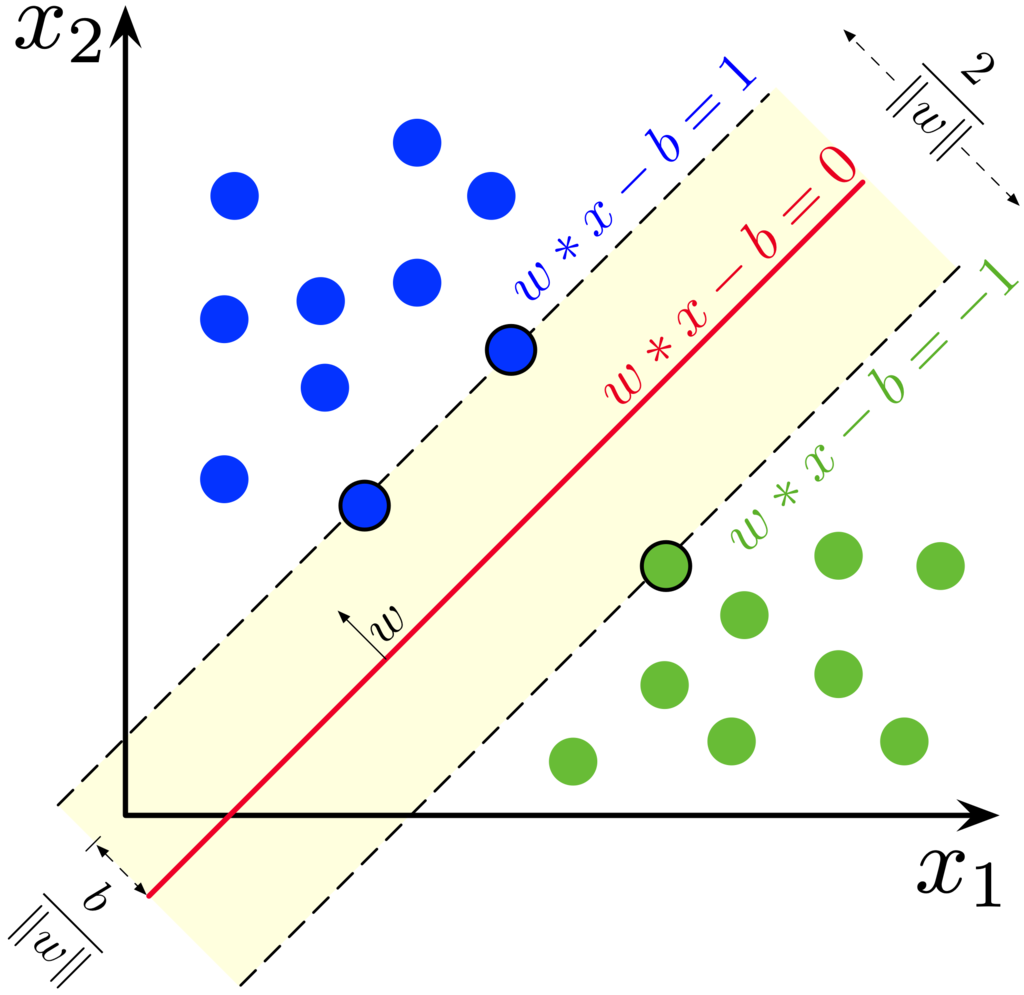
\includegraphics[width=0.4\linewidth]{fig/svm.png}
    \caption{Maximum Margin Hyperplan และ Margi สำหรับการฝึกสอนโมเดลของชุดข้อมูลตัวอย่างที่มี 2 คลาสด้วย Support Vector Machine (เครดิตภาพ: \url{https://en.wikipedia.org/wiki/Support_vector_machine})}
    \label{fig:svm_margin}
\end{figure}

ภาพที่ \ref{fig:svm_margin} แสดงชุดข้อมูลตัวอย่างที่มี 2 คลาส (สีน้ำเงินกับสีเขียว) โดยมีระนาบระยะห่างที่มากที่สุด (Maximum Margin Hyperplan หรือ MMH) เป็นตัวแบ่งข้อมูลซึ่งอ้างอิงโดยจุดข้อมูลที่อยู่ใกล้กับ Hyperplan ซึ่งจุดข้อมูลเหล่านี้มีชื่อเรียกว่าเวกเตอร์ค้ำยัน (Support Vector) โดยเราคำนวณ Support Vector จากช่องว่าง (Margin) ระหว่างคลาสทั้ง 2 คลาสโดยใช้ระยะห่างที่น้อยที่สุด ดังนั้นเป้าหมายของการฝึกสอนโมเดลด้วย SVM ก็คือการหา Hyperplan ที่สามารถแบ่งข้อมูลทั้ง 2 คลาสออกจากกันได้ดีที่สุด
\idxen{Supervised Learning!Support Vector Machine!Hyperplane}
\idxen{Supervised Learning!Support Vector Machine!Margin}

โค้ดด้านล่างคือตัวอย่างการเรียกใช้ฟังก์ชัน \inlinehighlight{svm} ของไลบรารี่ Scikit-Learn สำหรับการฝึกสอนโมเดลด้วย SVM โดยใช้ข้อมูลตัวอย่างที่สมมติขึ้นมา

\begin{lstlisting}[style=MyPython]
import numpy as np
from sklearn import svm

# Create dataset
x = np.arange(10).reshape(-1, 1)
y = np.array([0, 0, 0, 0, 1, 1, 1, 1, 1, 1])
x_test = x + 1.2

# Create a SVM classifier using linear kernel
clf = svm.SVC(kernel='linear')

# Train the model
clf.fit(x, y)

# Predict the response for test dataset
clf.predict(x_test)
# Output
array([0, 0, 0, 1, 1, 1, 1, 1, 1, 1])
\end{lstlisting}

%--------------------------
\section{เทคนิคการเรียนรู้แบบมีผู้สอนแบบอื่น ๆ}
\label{sec:other_ml}
\idxth{เทคนิคการเรียนรู้แบบผู้มีสอน}
\idxth{เทคนิคการเรียนรู้ของเครื่อง}
\idxen{Machine Learning Techniques}
\idxen{Unsupervised Machine Learning Techniques}
%--------------------------

%--------------------------
\subsection{Partial Least Squares (PLS)}
\label{ssec:pls}
\idxth{เทคนิคการเรียนรู้ของเครื่อง!วิธีกำลังสองน้อยที่สุดบางส่วน}
\idxen{Machine Learning Techniques!Partial Least Squares}
%--------------------------

วิธีกำลังสองน้อยที่สุดบางส่วน (Partial Least Squares หรือ PLS) เป็นวิธีเชิงสถิติที่ใช้สำหรับการวิเคราะห์หลายตัวแปรเพื่อสร้างตัวแบบความสัมพันธ์ระหว่างกลุ่มของตัวแปรทำนาย (Predictor Variable) โดยอาศัยตัวแปรแฝง (Latent variable) ซึ่งเทคนิคนี้มีความคล้ายกับ Principle Component Analysis (PCA) ซึ่งจะเป็นการลดจำนวนมิติของข้อมูล\autocite{wold1984} ในช่วงยุคเริ่มต้นที่มีการใช้ปัญญาประดิษฐ์ในงานด้านเคมีนั้น เทคนิคนี้ได้ถูกนำมาใช้อย่างแพร่หลาย เช่น นำมาใช้สำหรับการระบุ Vibrational Bands สำหรับ Vibrational Spectra และนำผลที่ได้มาเปรียบเทียบกับค่าการทำนายที่ได้จากวิธีอื่น เช่น ANN และ PCA-ANN

%--------------------------
\subsection{Gaussian Process Regression (GPR)}
\label{ssec:gpr}
\idxth{เทคนิคการเรียนรู้ของเครื่อง!การถดถอยของกระบวนการเกาส์เซียน}
\idxen{Machine Learning Techniques!Gaussian Process Regression}
%--------------------------

การถดถอยของกระบวนการเกาส์เซียน (Gaussian Process Regression หรือ GPR) เป็นวิธีการถดถอยของเบส์แบบหนึ่งโดยใช้ Kernel Function ที่สามารถบ่งบอกหรือแสดงค่าความแปรปรวน (Covariance) ในขั้นตอน Gaussian Process ได้\autocite{rasmussen2005} โดย GPR จะทำการสร้างโมเดลแบบ Non-parametric และสามารถคำนวณค่าความเชื่อมั่น (Confidence Intervals) ไปพร้อม ๆ กับการทำนาย รายละเอียดเพิ่มเติมของ GPR สามารถศึกษาได้ในหัวข้อ \ref{sec:gaussian_process}

%--------------------------
\subsection{Random Forest}
\label{ssec:rs}
\idxth{เทคนิคการเรียนรู้ของเครื่อง!เครื่องเวกเตอร์ค้ำยัน}
\idxen{Machine Learning Techniques!Random Forest}
%--------------------------

การสุ่มป่าไม้ (Random Forest หรือ RF) เป็นวิธีหนึ่งในกลุ่มของโมเดลที่เรียกว่าการเรียนรู้แบบกลุ่มก้อน (Ensemble Learning) ที่มีหลักการคือการฝึกสอนโมเดลที่เหมือนกันหลาย ๆ ครั้ง (Multitude) บนข้อมูลชุดเดียวกัน โดยแต่ละครั้งของการเทรนจะเลือกส่วนของข้อมูลที่ฝึกสอนไม่เหมือนกัน แล้วนำการตัดสินใจของโมเดลเหล่านั้นมาโหวตเลือกกันว่า Class ไหนถูกเลือกมากที่สุด\autocite{breiman2001,quinlan1986}

\noindent ตัวอย่างการเขียนโค้ดโมเดล Random Forest สำหรับการทำ Regression
%
\begin{lstlisting}[style=MyPython]
from sklearn.ensemble import RandomForestRegressor
from sklearn.datasets import make_regression

X, y = make_regression(n_features=4, n_informative=2,
                       random_state=0, shuffle=False)
regr = RandomForestRegressor(max_depth=2, random_state=0)
regr.fit(X, y)

print(regr.predict([[0, 0, 0, 0]]))
# Output
[-8.32987858]
\end{lstlisting}

\vspace{1em}

\noindent ตัวอย่างการเขียนโค้ดโมเดล Random Forest สำหรับการทำ Classification
%
\begin{lstlisting}[style=MyPython]
from sklearn.ensemble import RandomForestClassifier
from sklearn.datasets import make_classification

X, y = make_classification(n_samples=1000, n_features=4,
                           n_informative=2, n_redundant=0,
                           random_state=0, shuffle=False)
clf = RandomForestClassifier(max_depth=2, random_state=0)
clf.fit(X, y)

print(clf.predict([[0, 0, 0, 0]]))
# Output
[1]
\end{lstlisting}

%--------------------------
\subsection{Artificial Neural Network}
\label{ssec:ann}
\idxth{เทคนิคการเรียนรู้ของเครื่อง!โครงข่ายประสาทเทียมประดิษฐ์}
\idxen{Machine Learning Techniques!Artificial Neural Network}
%--------------------------

โครงข่ายประสาทเทียมประดิษฐ์ (Artificial Neural Network หรือ ANN) หรือเรียกว่าโครงข่ายประสาทเทียม (Neural Network หรือ Neural Net) เป็นอัลกอริทึมรูปแบบหนึ่งที่เลียนแบบการทำงานของสมองมนุษย์ โดยทำการสร้างโมเดลเรียนรู้ที่ประกอบไปด้วยชั้นเรียนรู้ระหว่างกลาง (Hidden Layer) และหน่วยย่อยที่เกิดการเรียนรู้ (Node หรือ Artificial Neuron หรือ Unit)

\begin{figure}[H]
    \centering
    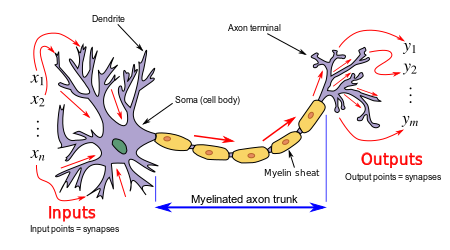
\includegraphics[width=0.8\linewidth]{fig/neuron.png}
    \caption{การรับส่งข้อมูลภายในเซลล์ประสาท (เครดิตภาพ: https://en.wikipedia.org/wiki/Biological\_neuron\_model)}
    \label{fig:neuron}
\end{figure}

จริง ๆ แล้ว Neural Network ก็คือการจำลองสมองมนุษย์โดยพยายามสร้างองค์ประกอบต่าง ๆ ให้มีความคล้ายกันให้มากที่สุด เช่น ในสมองมีเซลล์ประสาท (Neurons) และจุดประสานประสาท (Synapses) แต่ละเซลล์ประสาทประกอบด้วยปลายในการรับกระแสประสาทเรียกว่า \enquote{เดนไดรท์} (Dendrite) ซึ่งเป็นอินพุตและปลายในการส่งกระแสประสาทเรียกว่าแอคซอน (Axon) ซึ่งเปรียบเหมือนเป็นเอาต์พุตของเซลล์

โดยโมเดล Neural Network ที่มีการนำไปใช้มากที่สุดคือเครือข่ายประสาทแบบป้อนไปหน้า (Feed-Forward Network) และโมเดล Neural Network ยังสามารถแบ่งออกได้เป็นหลายประเภท ดังนี้
%
\begin{itemize}[topsep=0pt,noitemsep]\setlength\itemsep{0.5em}
    \item เพอร์เซ็ปตรอนชั้นเดียว (Single-layer Perceptron)

    \item เพอร์เซ็ปตรอนหลายชั้น (Multi-layer Perceptron)

    \item โครงข่ายแบบวนซ้ำ (Recurrent Neural Network)

    \item แผนผังจัดระเบียบเองได้ (Self-organizing Map)

    \item เครื่องจักรโบลทซ์แมน (Boltzmann Machine)

    \item กลไกแบบคณะกรรมการ (Committee of Machines)

    \item โครงข่ายความสัมพันธ์ (Associative Neural Network)

    \item โครงข่ายกึ่งสำเร็จรูป (Instantaneously Trained Networks)

    \item โครงข่ายแบบยิงกระตุ้น (Spiking Neural Networks)
\end{itemize}

โดยในหนังสือเล่มนี้จะอธิบายเฉพาะ Neural Network แบบเพอร์เซ็ปตรอนชั้นเดียวและเพอร์เซ็ปตรอนหลายชั้น (บทที่ \ref{ch:deep_learning}) สำหรับผู้อ่านที่สนใจศึกษารายละเอียดของ Neural Network ประเภทอื่น สามารถศึกษาได้จากหนังสือเฉพาะทาง เช่น \enquote{Deep Learning} เขียนโดย Ian Goodfellow, Yoshua Bengio และ Aaron Courville\autocite{Goodfellow-et-al-2016} รายละเอียดเพิ่มเติมดูได้ที่เว็บไซต์ \url{https://www.deeplearningbook.org}
 % การเรียนรู้แบบมีผู้สอน
% LaTeX source for ``การเรียนรู้ของเครื่องสำหรับเคมีควอนตัม (Machine Learning for Quantum Chemistry)''
% Copyright (c) 2022 รังสิมันต์ เกษแก้ว (Rangsiman Ketkaew).

% License: Creative Commons Attribution-NonCommercial-NoDerivatives 4.0 International (CC BY-NC-ND 4.0)
% https://creativecommons.org/licenses/by-nc-nd/4.0/

\chapter{วิธีเคอร์เนล}
\label{ch:kernel}

%--------------------------
\section{เคอร์เนลคืออะไร}
\label{sec:kernel}
\idxboth{เคอร์เนล}{Kernel}
%--------------------------

ในบทที่แล้วเราได้เรียนรู้เทคนิค Linear Regression (การถดถอยแบบเส้นตรง) กันไปแล้ว ซึ่งเป็นกรณีที่เราเจอปัญหาที่เกี่ยวข้องกับความสัมพันธ์%
ของตัวแปรสองตัว โดยเราสามารถทำการ Fit สมการเชิงเส้นของอินพุต $(x)$ ให้เข้ากับชุดข้อมูล (Training Data) แล้วถ้าหากค่าเอาต์พุต 
$(y)$ ที่เราต้องการทำนายนั้นสามารถถูกทำนายหรืออธิบายได้ดีกว่าด้วยสมการไม่เชิงเส้น (Nonlinear Function) ของตัวแปร $x$ นั้น 
เราสามารถใช้สิ่งที่เรียกว่าเคอร์เนล (Kernel) ในการหาความสัมพันธ์ระหว่างอินพุตกับเอาต์พุตได้ ซึ่งเราจะมาทำความรู้จักและเรียนรู้เคอร์เนลกันในบทนี้ 

\begin{figure}[htbp]
    \centering
    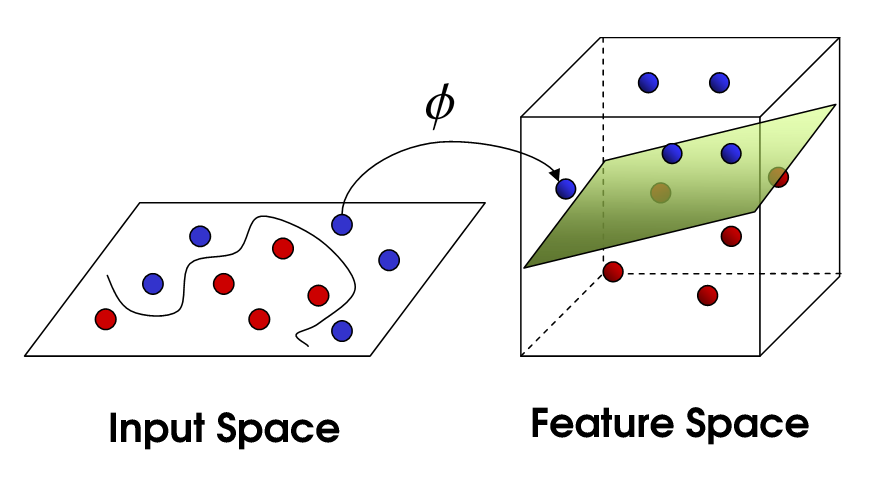
\includegraphics[width=0.8\linewidth]{fig/2d_to_3d_spaces.png}
    \caption{การทำ Mapping จากปริภูมิ 2 มิติไปเป็นปริภูมิ 3 มิติซึ่ง Observation ของเราสามารถถูกแยกได้โดยฟังก์ชันเชิงเส้น}
    \label{fig:2d_to_3d}
\end{figure}

ถ้าสมมติว่าผู้เขียนเริ่มต้นด้วยการยกสมการทางคณิตศาสตร์มาอธิบายว่าเคอร์เนลคืออะไร ผู้อ่านหลายท่านก็อาจจะสับสนได้ ดังนั้นผู้จึงขอยกเริ่มต้นด้วย%
การอธิบายง่าย ๆ แบบนี้ว่าถ้าสมมติเรามีชุดข้อมูลที่อยู่ในปริภูมิ 2 มิติ (2-dimensional Space) หรือที่เรียกว่า Input Space ดังที่แสดงในภาพที่ 
\ref{fig:2d_to_3d} เราจะพบว่าเราไม่สามารถหาฟังก์ชันเชิงเส้นที่สามารถแยกข้อมูลจุดสีแดงออกจากสุดสีน้ำเงินได้ แต่ถ้าหากเราแปลงข้อมูล%
จากปริภูมิ 2 มิติให้ไปอยู่ในปริภูมิ 3 มิติซึ่งเราจะเรียกปริภูมินี้ว่า Feature Space ตามรูปทางด้านขวา เราพบว่าข้อมูลของเราหลังจากที่ถูกแปลงนั้น%
จะสามารถถูกแยกออกจากกันได้ด้วยฟังก์ชันเชิงเส้น (ในที่นี้คือระนาบที่แบ่งข้อมูลทั้งสองคลาสออกจากกัน) ซึ่งกระบวนการนี้เรียกว่า Mapping 
หลังจากนั้นให้เราทำ Mapping อีกครั้งหนึ่งโดยแปลงย้อนกลับไปสู่ปริภูมิ 2 มิติ ซึ่งผลลัพธ์ที่ได้จะเป็นฟังก์ชันแบบไม่เชิงเส้นที่อยู่ในมิติที่ต่ำลงนั่นเอง 
\idxen{Mapping}

สรุปสั้น ๆ คือวิธีเคอร์เนลเป็นการประยุกต์ใช้ฟังก์ชันเชิงเส้นกับปัญหาที่เป็นแบบไม่เชิงเส้นโดยการแปลงข้อมูลให้อยู่ในปริภูมิที่มีมิติที่สูงขึ้น (อาจจะ 3 
มิติหรือสูงกว่านี้ก็ได้) โดยที่เราไม่จำเป็นที่จะต้องเข้าใจปริภูมิมิติสูงเหล่านั้น (จริง ๆ แล้วถ้าเราเข้าใจได้ก็ดี แต่ว่าการอธิบายปริมาณทางคณิตศาสตร์%
ที่มีจำนวนมิติมากกว่าสามมิตินั้นเป็นสิ่งที่เข้าใจได้ยาก)

%--------------------------
\section{คณิตศาสตร์ของเคอร์เนล}
\label{sec:math_kernel}
%--------------------------

ก่อนที่เราจะลงลึกไปที่ตัวทฤษฎีของเคอร์เนลนั้น เราควรจะต้องมาทำความเข้าใจสิ่งที่เป็นพื้นฐานกันก่อนนั่นก็คือ Feature Map ซึ่งเป็นสิ่งที่ทำการ%
เชื่อมโยง Attribute ให้เข้ากับ Feature ซึ่งเราเรียกกระบวนการนี้ว่า Mapping ตามที่ได้อธิบายไปก่อนหน้านี้

เริ่มต้นด้วยการพิจารณาการ Fit ฟังก์ชันแบบ Cubic Function โดยสมการดังนี้

\begin{equation}\label{eq:cubic_func}
    y = \theta_{3}x^{3} + \theta_{2}x^{2} + \theta_{1}x^{1} + \theta_{0}
\end{equation}

\noindent จะเห็นได้ว่าเราสามารถที่จะมอง Cubic Function ด้านบนเป็นสมการเชิงเส้นง่าย ๆ ซึ่งสมการ \ref{eq:cubic_func} นั้นจะขึ้น%
อยู่กับ Feature Variables $(x)$ ที่เรากำหนดไว้นั่นเอง คราวนี้เราลองมากำหนดฟังก์ชันใหม่โดยอ้างอิงสมการเดิม ซึ่งเราจะมีการกำหนดเซต%
ของตัวแปร $x$ ตัวใหม่ขึ้นมานั่นคือ

\begin{align}\label{eq:cubic_func_2}
    y &= \theta_{3}x^{3} + \theta_{2}x^{2} + \theta_{1}x^{1} + \theta_{0} \nonumber \\ 
      &= \theta^{\top}\phi(x)
\end{align}

\noindent โดยที่ $\phi$ คือเวกเตอร์ของตัวแปรอินพุต ดังนี้

\begin{equation}
\phi = 
\begin{bmatrix}
    1 \\
    x \\
    x^{2} \\
    x^{3} 
\end{bmatrix}
\end{equation}

\noindent และ $\theta^{\top}$ เป็นเวกเตอร์ของพารามิเตอร์ $\theta_{i}$ ดังนี้

\begin{equation}
\theta^{\top} =
\begin{bmatrix}
    \theta_{o} & \theta_{1} & \theta_{2} & \theta_{3}
\end{bmatrix}
\end{equation}

\noindent ซึ่งทั้งสองเวกเตอร์นี้ก็คูณกันแบบ Dot Product ตามสมการที่ \ref{eq:cubic_func_2}
 
คำถามที่ตามมาก็คือเราจะแยกความแตกต่างระหว่างสมการ \ref{eq:cubic_func} กับ \ref{eq:cubic_func_2} ได้อย่างไร คำตอบก็คือเรา%
สามารถทำได้โดยการกำหนดให้ตัวแปรอินพุต $x$ ของเรานั้นเป็น Attribute เมื่อเราทำการ Map หรือเชื่อมโยงตัวแปร $x$ ของเราไปยังปริมาณ%
ตัวใหม่ที่เป็น $\phi(x)$ เราจะเรียกปริมาณตัวนี้ว่า Feature และฟังก์ชันที่เราใช้ในการ Mapping นั้นเราเรียกว่า Feature Map $(\phi)$ 
ซึ่งเป็นตัวที่ทำการเชื่อมโยงความสัมพันธ์ของ Attribute ไปยัง Feature ตามที่ได้เกริ่นไว้ก่อนหน้านี้

ดังนั้นโจทย์ของเราในการทำ Regression ก็คือการหาอัลกอริทึม Gradient Descent ที่จะนำมาใช้ในการ Fitting โมเดลของเรา (อันที่จริงแล้ว
$\theta^{\top}\phi(x)$ ก็คือโมเดลของเรานั่นเอง) โดยหนึ่งในอัลกอริทึมที่สามารถนำมาใช้ในการ Fitting ได้อย่างมีประสิทธิภาพก็คือ 
Stochastic Gradient Descent ซึ่งมีสมการดังต่อไปนี้

\begin{equation}\label{eq:sto_grad_des}
    \theta := \theta + \alpha (y^{i} - \theta^{\top}\phi(x^{i}))\phi(x^{i})
\end{equation}

\noindent โดยที่ $\alpha$ คือขนาดของการก้าวเดิน (Step Size) หรืออัตราเร็วของการเรียนรู้ (Learning Rate) ซึ่งเป็นพารามิเตอร์ที่จะ%
ปรับความเร็วในการปรับความเหมาะสม (Optimize) เกรเดียนต์ (สำหรับรายละเอียดเพิ่มเติมเกี่ยวกับการพิสูจน์สมการที่ \ref{eq:sto_grad_des} 
ผู้อ่านสามารถอ่านได้จากหนังสือปัญญาประดิษฐ์) อย่างไรก็ตาม ปัญหาอย่างหนึ่งของ Stochastic Gradient Descent นั้นก็คือไม่สามารถที่จะ%
หาผลเฉลยได้ง่าย จึงทำให้การฝึกสอนโมเดลนั้นมีความสิ้นเปลืองในการคำนวณเป็นอย่างมาก (Computationally Expensive) โดยเฉพาะอย่าง%
ยิ่งเมื่อ Feature ของเรา $(\phi(x))$ นั้นมีจำนวนมิติที่เยอะมาก ๆ (ผู้อ่านสามารถศึกษารายละเอียดของ Stochastic Gradient Descent 
ได้ในหัวข้อที่ \ref{ssec:stochastic_grad})

สำหรับนิยามของเคอร์เนล $(K)$ นั้นจริง ๆ แล้วมีหลายนิยามมาก ขึ้นอยู่กับว่าต้องการจะให้นิยามในบริบททางคณิตศาสตร์หรือสถิติ โดยส่วนตัวของ%
เขียนนั้นคิดว่าเคอร์เนลเป็นวิธีทางสถิติที่เกี่ยวข้องกับการหาความเชื่อมโยงระหว่างตัวแปรสองตัว ซึ่งความเชื่อมโยงในที่นี้ก็คือความคล้ายคลึงกัน 
(Similarity) ผู้อ่านบางท่านอาจจะเคยได้ยินหรือเคยใช้วิธี เช่น Jaccard Similarity หรือ Cosine Similarity มาก่อนบ้าง 

คราวนี้เรามาดูนิยามทางคณิตศาสตร์ของเคอร์เนลกันครับ เริ่มต้นกำหนดเคอร์เนลให้อยู่ในรูปของ Feature Map $(\phi)$ ซึ่งเป็นฟังก์ชันที่ทำการ 
Mapping ปริภูมิของตัวแปรอินพุต $x$ ที่ได้อธิบายไว้ก่อนหน้านี้ $(\chi \times \chi \rightarrow \mathbb{R})$ ดังนี้

\begin{equation}\label{eq:kernel}
    K(x,z) = \langle\phi(x),\phi(z)\rangle
\end{equation}

\noindent ซึ่งเราสามารถคำนวณ $\langle\phi(x),\phi(z)\rangle$ ได้โดยการใช้สมการต่อไปนี้

\begin{align}
    \langle\phi(x),\phi(z)\rangle =& 1 + \sum_{i=1}^d x_i z_i + 
    \sum_{i,j\in\{1,\ldots,d\}} x_i x_j z_i z_j \nonumber \\
    &+ \sum_{i,j,k \in \{1,\ldots,d\}} x_i x_j x_k z_i z_j z_k \\
    =& 1 + \sum_{i=1}^d x_i z_i + \left(\sum_{i=1}^d x_i z_i \right)^2 + \left( \sum_{i=1}^d x_i z_i \right)^3 \\
    =& 1 + \langle x,z \rangle + \langle x,z \rangle^2 + \langle x,z \rangle^3\label{eq:feat_map_inner_product}
\end{align}

\noindent อธิบายง่าย ๆ ก็คือเราจะคำนวณพจน์แรก $\langle x,z \rangle$ ของสมการ \ref{eq:feat_map_inner_product} ก่อน 
หลังจากนั้นจึงคำนวณพจน์อื่น ๆ ที่เหลือ (กำหนดให้ $i,j$ เป็นสมาชิกของเซต $\{1, \dots, n\})$

%--------------------------
\section{ฟังก์ชันเคอร์เนลและคุณสมบัติของเคอร์เนล}
\label{sec:func_kernel}
\idxboth{เคอร์เนล!ฟังก์ชันเคอร์เนล}{Kernel!Function Kernel}
\idxen{Kernel!Kernel Properties}
%--------------------------

ในหัวข้อนี้เราจะมาดูรายละเอียดของเคอร์เนลกันว่า $K(x,z)$ มีคุณสมบัติอะไรที่น่าสนใจบ้าง สำหรับสัญลักษณ์ที่เราจะกำหนดขึ้นมาเพื่ออธิบาย%
เคอร์เนลนั้นจะเป็น $K(\cdot,\cdot)$ หรือเรียกง่าย ๆ ว่าเป็นฟังก์ชันเคอร์เนล (Kernel Function) ก็ได้ ผู้เขียนขอยกตัวอย่างของฟังก์ชัน%
เคอร์เนลแบบเรียบง่ายให้ดูกันก่อน ดังนี้

\begin{equation}
    K(x,z) = (x^{\top} z)^{2}
\end{equation}

\noindent ซึ่งเราสามารถจัดรูปสมการใหม่ได้เป็น

\begin{align}
    K(x,z) &= \left( \sum_{i=1}^d x_i z_i \right) \left( \sum_{j=1}^d x_j z_j \right)\\
    &= \sum_{i=1}^d \sum_{j=1}^d x_i x_j z_i z_j\\
    &= \sum_{i,j=1}^d (x_i x_j)(z_i z_j)
\end{align}

\noindent ซึ่งจะเห็นได้ชัดเลยว่าจริง ๆ แล้วนั้น $K(x,z) = \langle\phi(x),\phi(z)\rangle$ เป็นฟังก์ชันเคอร์เนลที่สอดคล้องกับ Feature 
Mapping $(\phi)$ โดยตัวอย่างเช่น กรณีที่ $d = 3$ นั้นมีสมการเป็น

\begin{equation}\label{eq:feature_map_ex1}
    \phi(x) = \begin{bmatrix}
    x_1 x_1\\
    x_1 x_2\\
    x_1 x_3\\
    x_2 x_1\\
    x_2 x_2\\
    x_2 x_3\\
    x_3 x_1\\
    x_3 x_2\\
    x_3 x_3\\
    \end{bmatrix}
\end{equation}

เราลองมาดูตัวอย่างที่สองของ $K(\cdot,\cdot)$ ซึ่งถูกกำหนดด้วยฟังก์ชันเชิงเส้นดังต่อไปนี้

\begin{align}
    K(x,z) &= (x^{\top} z + c)^2\\
    &= \sum_{i,j=1}^d (x_i x_j)(z_i z_j) + \sum_{i=1}^d \left(\sqrt{2c}x_i\right) \left(\sqrt{2c}z_i\right) 
    + c^2
\end{align}

\noindent โดยที่ฟังก์ชันเคอร์เนลด้านบนนี้ก็จะคล้าย ๆ กับก่อนหน้านี้แต่จะมีความแตกต่างตรงที่มีการเพิ่มพารามิเตอร์ $c$ เข้ามา ซึ่งเป็นสิ่งที่%
กำหนดการถ่วงน้ำหนัก (Weighting) ระหว่าง $x_{i}$ และ $x_{i}x_{j}$ โดยที่เรามองได้ง่าย ๆ ก็คือเคอร์เนล $K(x,z) = (x^{\top} 
z + c)^2$ นั้นจะมีความสอดคล้องกับ Feature Mapping ไปยังปริภูมิของ $\binom{d+k}{k}$ โดยที่ Feature Mapping ของกรณีนี้ที่ 
$d = 3$ นั้นมีสมการดังต่อไปนี้

\begin{equation}\label{eq:feature_map_ex2}
    \phi(x) = \begin{bmatrix}
        x_1 x_1\\
        x_1 x_2\\
        x_1 x_3\\
        x_2 x_1\\
        x_2 x_2\\
        x_2 x_3\\
        x_3 x_1\\
        x_3 x_2\\
        x_3 x_3\\
        \sqrt{2c}x_1\\
        \sqrt{2c}x_2\\
        \sqrt{2c}x_3\\
        c
    \end{bmatrix}
\end{equation}

\begin{figure}[htbp]
    \centering
    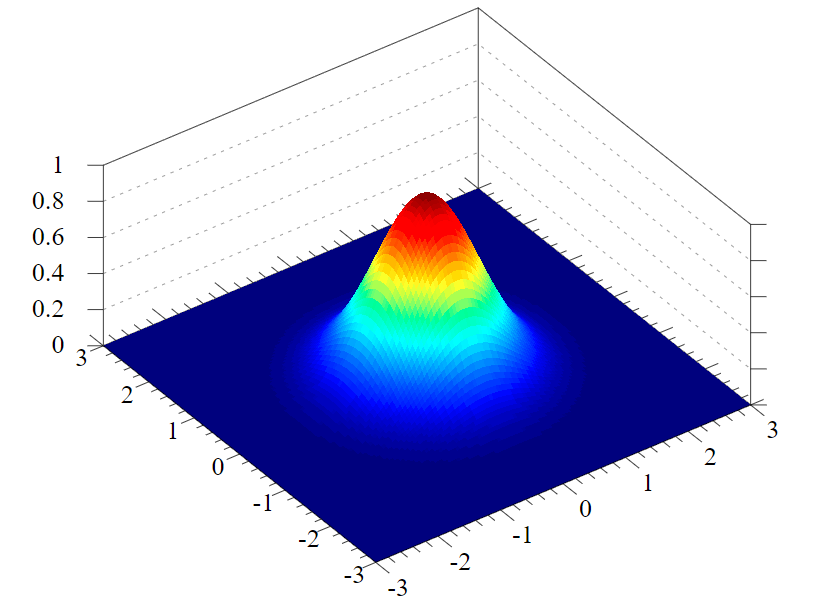
\includegraphics[width=0.9\linewidth]{fig/gaussian-3d.png}
    \caption{ตัวอย่างพื้นผิวการกระจายตัวเกาส์เซียน (Gaussian Distribution) ในปริภูมิ 3 มิติ}
    \label{fig:gaussian_3d}
\end{figure}

คราวนี้เราลองมามองเคอร์เนลให้เป็นเมตริกหรือตัววัดความคล้ายคลึงกันระหว่าง Feature Mapping (Similarity Metrics) เราเริ่มต้นด้วย%
สมมติฐานที่ว่าถ้ากรณีที่ $\phi(x)$ กับ $\phi(z)$ บนปริภูมินั้นมีความใกล้กันมาก ๆ เราอาจจะคาดการณ์ได้ว่า $K(x,z) = \phi(x)^{\top} 
\phi(z$ จะมีขนาดที่ใหญ่มากเพราะว่ามีการซ้อนทับกันเยอะ (เรานิยามให้การซ้อนทับกันหรือ Overlap นั้นเป็นความคล้ายคลึงกัน) แต่ในกรณีที่%
ตรงข้ามกัน ถ้าหาก $\phi(x)$ กับ $\phi(z)$ อยู่ห่างกันมากก็จะทำให้การ Overlap นั้นมีน้อย จึงทำขนาดของเคอร์เนล $K(x,z) = 
\phi(x)^{\top} \phi(z)$ มีขนาดที่เล็กลงตามไปด้วย ซึ่งการที่เราสามารถนิยามเคอร์เนลให้เป็นมาตรวัดความคล้ายคลึงกันระหว่าง $x$ และ 
$z$ นั้นมีประโยชน์อย่างมาก เพราะเราสามารถนำไปแก้ปัญหาหลาย ๆ อย่างได้ แต่ว่าฟังก์ชันที่เราเลือกมาใช้ในการอธิบายความแตกต่างของทั้งสอง%
ตัวแปรนั้นจะต้องมีความสมเหตุสมผล โดยฟังก์ชันที่ได้รับความนิยมในการนำมาใช้เป็นฟังก์ชันเคอร์เนลนั้นก็คือฟังก์ชันเกาส์เซียน (Gaussian 
Function) หรือเรียกอีกอย่างว่า Radial BasisFunction (RBF) ตามภาพที่ \ref{fig:gaussian_3d} ซึ่งมีสมการดังต่อไปนี้ 

\begin{equation}\label{eq:rbf_kernel}
    K(x,z) = \exp\left(-\frac{\lVert x - z \rVert^2}{2\sigma^2}\right)   
\end{equation}

\noindent โดยที่ $\sigma$ คือไฮเปอร์พารามิเตอร์ (Hyperparameter) ที่กำหนดความเรียบเนียน (Smoothness) ของขอบเขตการตัดสินใจ 
(Decision Boundary) และ $\lVert x - z \rVert^2$ คือระยะห่างยูคลิเดียนยกกำลังสอง (Squared Euclidean Distance) ระหว่าง 
Feature Vector $x$ และ $z$ ซึ่งสามารถหาค่าได้โดยใช้สมการดังต่อไปนี้

\begin{align}
    d(x_{i}, x_{k}) &= 
    \sqrt{(x^{(1)}_{i} - x^{(1)}_{k})^{2} + (x^{(2)}_{i} - x^{(2)}_{k})^{2} + \cdots + 
    (x^{(N)}_{i} - x^{(N)}_{k})^{2}} \\
    &= \sqrt{\sum^{N}_{n=1} (x^{(n)}_{i} - x^{(n)}_{k})^{2}}
\end{align}

ฟังก์ชันในสมการ \ref{eq:rbf_kernel} นั้นเมื่อถูกนำมาใช้เป็นเคอร์เนลแล้วเราจะเรียกเคอร์เนลนี้ว่าเคอร์เนลเกาส์เซียน (Gaussian Kernel)
ซึ่งเป็นฟังก์ชันที่เหมาะสมมาก ๆ เพราะว่ามีความสมมาตร มีความต่อเนื่องตลอดช่วงของปริภูมิ และมีค่าเข้าใกล้ 1 เมื่อ $x$ และ $z$ นั้นอยู่ใกล้กัน 
แต่จะมีค่าเข้าใกล้ 0 เมื่อ $x$ และ $z$ อยู่ห่างกัน

เรามาดูการเขียนโค้ดสำหรับการ Mapping ด้วยวิธีเคอร์เนลกันครับ เริ่มต้นด้วยโค้ดที่กำหนดชุดข้อมูลตัวอย่างซึ่งเป็นแบบไม่เป็นเชิงเส้น ดังนี้

\begin{lstlisting}[style=MyPython]
import numpy as np
import matplotlib.pyplot as plt

# Kernel
x = np.array([1,1,2,3,3,6,6,6,9,9,10,11,12,13,16,18])
y = np.array([18,13,9,6,15,11,6,3,5,2,10,5,6,1,3,1])
label = np.array([1,1,1,1,0,0,0,1,0,1,0,0,0,1,0,1])

# Plot
fig = plt.figure()
plt.scatter(x, y, c=label, s=60)
plt.show()
\end{lstlisting}

\noindent เขียนฟังก์ชันสำหรับการ Mapping ดังนี้

\begin{lstlisting}[style=MyPython]
def mapping(x, y):    
	x = np.c_[(x, y)]				
    if len(x) >	2:        
    	x_1 = x[:,0]**2        
        x_2 = np.sqrt(2)*x[:,0]*x[:,1]        
        x_3 = x[:,1]**2								
    else:            
    	x_1 = x[0]**2        
        x_2 = np.sqrt(2)*x[0]*x[1]        
        x_3 = x[1]**2			    
    trans_x = np.array([x_1, x_2, x_3])				
    return trans_x	
\end{lstlisting}

\noindent แล้วทำการ Mapping, แสดงผลลัพธ์ และพล็อตข้อมูลหลังจาก Mapping

\begin{lstlisting}[style=MyPython]
# Mapping
x_1  = mapping(x, y)
x_1.shape
# Output
(3, 15)

# Plot
fig = plt.figure()
ax = fig.add_subplot(111, projection='3d')
ax.scatter(x_1[0], x_1[1], x_1[2], c=label, s=60)
ax.view_init(30, 185)
ax.set_xlabel('X Label')
ax.set_ylabel('Y Label')
ax.set_zlabel('Z Label')
plt.show()
\end{lstlisting}

โดยสรุปก็คือเคอร์เนลเป็นเทคนิคอย่างหนึ่งที่ช่วยให้เราสามารถทรานฟอร์มหรือแปลงข้อมูล (Transform) จากปริภูมิมิติต่ำ (Low-dimensional 
Space) ไปยังปริภูมิมิติสูง (High-dimensional Space) ซึ่งฟังก์ชันที่เหมาะสมที่สุดที่เราสามารถเลือกมาใช้เป็นฟังก์ชันเคอร์เนลได้นั้นไม่มีใครรู้%
ว่ามีหน้าตาเป็นอย่างไร ดังนั้นการที่เราจะทำ Mapping โดยเลือกใช้ทุกฟังก์ชันนั้นจึงแทบจะเป็นไปไม่ได้เลยเพราะว่ามีขีดจำกัดด้านการคำนวณ

%--------------------------
\subsection{การถดถอยแบบเชิงเส้น}
\label{ssec:lin_reg}
\idxen{Kernel!Linear Regression}
%--------------------------

กรณีแบบแรกของการถดถอย (Regression) ก็คือการถดถอยแบบเชิงเส้น (Linear Regression) ซึ่งเราได้ศึกษากันไปแล้วในหัวข้อที่ 
\ref{sec:lin_res} ของบทที่ \ref{ch:sup_ml} ซึ่งเราใช้สมการดังต่อไปนี้ในการแก้ปัญหาการปรับค่าลงให้ต่ำที่สุด (Minimization)

\begin{equation}
    \min_{w} \lVert X_{w} - y \rVert_{2}^{2}
\end{equation}

\begin{figure}[htbp]
    \centering
    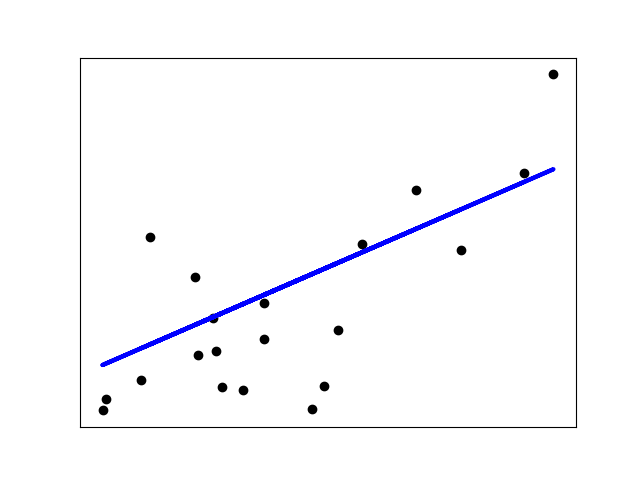
\includegraphics[width=0.8\linewidth]{fig/plot_linear_regression.png}
    \caption{เส้นตรงที่ถูก Fit (สมดุล) ให้ผ่านจุดในชุดข้อมูล แกน $x$ คืออินพุตและแกน $y$ คือเอาต์พุต (เครดิตภาพ: 
    https://scikit-learn.org)}
    \label{fig:lin_res}
\end{figure}

รูปที่ \ref{fig:lin_res} แสดงเส้นตรงที่เกิดจากการทำ Minimization ของสมการถดถอยแบบเชิงเส้น เส้นตรงสีน้ำเงินเส้นนี้ถูกปรับระยะห่าง%
เฉลี่ยระหว่างจุดทุกจุดในชุดข้อมูลโดยที่มีความสมดุลมากที่สุด โดยสังเกตด้วยตาเปล่าได้คร่าว ๆ ว่าแนวโน้มของจุดนั้นจะมีแนวโน้มที่เป็นแบบเอียง%
และชันขึ้นจากทางด้านซ้ายไปยังด้านขวา ดังนั้นเส้นตรงที่ได้จากการ Fit นั้นจึงมีแนวโน้มไปในทางเดียวกันซึ่งมีความชันเป็นบวกนั่นเอง

%--------------------------
\subsection{การถดถอยแบบริดจ์}
\label{ssec:ridge_reg}
\idxth{การถดถอย!การถดถอยแบบริดจ์}
\idxen{Kernel!Ridge Regression}
%--------------------------

สำหรับวิธีการถดถอยแบบริดจ์ (Ridge Regression) นั้นอาจจะมองได้ว่าเป็นการยกระดับ (Upgrade) หรือปรับปรุง Linear Regression 
ในกรณีที่เป็นแบบสามัญ (Ordinary) ให้มีประสิทธิภาพมากขึ้น นั่นก็เพราะว่ากรณีที่เราจะต้องทำการ Fit ข้อมูลที่มีจำนวนหลายตัวแปรและมีการ%
กระจายในแบบที่ไม่สามารถอธิบายได้ด้วยสมการเส้นตรงนั้น เรามีเทคนิคก็คือการใส่พจน์พิเศษเข้าไป ซึ่งวิธีนี้เรียกว่าเป็นการลงโทษ (Penalize) 
ซึ่งเป็นหนึ่งในรูปแบบของการทำ Regularization โดยมีรูปสมการทั่วไปดังต่อไปนี้

\begin{equation}
    \min_{w} \lVert X_{w} - y \rVert_{2}^{2} + \alpha \lVert w \rVert_{2}^{2}
\end{equation}

\noindent โดยพระเอกของเราใน Ridge Regression นั้นก็คือพจน์สุดท้ายซึ่งมีศัพท์ทางเทคนิคที่เรียกว่า $L2$ Regularization โดยมี%
พารามิเตอร์ที่สำคัญนั่นก็คือ $\alpha$ ซึ่งเป็นตัวปรับจำนวนการหด (Schrinkage) ของฟังก์ชัน ซึ่งคูณอยู่กับค่าขนาดของน้ำหนัก (Weight) 
ยกกำลังสอง ซึ่งการยกกำลังนี้เป็นที่มาของการเรียกว่า $L2$ นั่นเอง สำหรับวิธีการปรับค่า $\alpha$ และผลกระทบที่เกิดขึ้นนั้นสามารถดูได้ตามรูปที่ 
\ref{fig:ridge_res}

\begin{figure}[htbp]
    \centering
    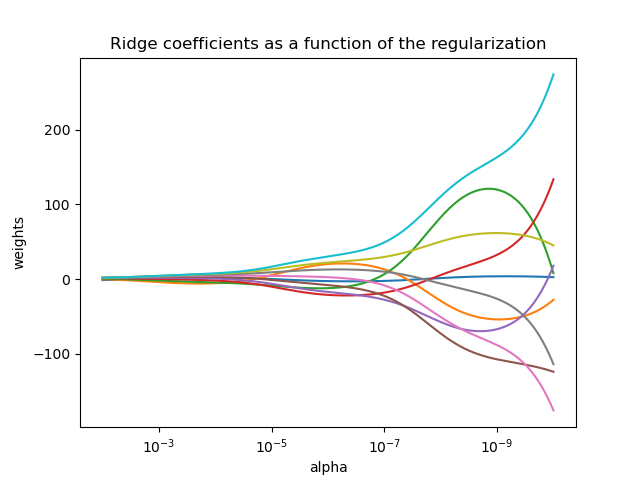
\includegraphics[width=0.9\linewidth]{fig/plot_ridge_regression.png}
    \caption{สัมประสิทธิ์ของริดจ์ที่เป็นฟังก์ชันกับ Regularization (เครดิตภาพ: https://scikit-learn.org)}
    \label{fig:ridge_res}
\end{figure}

\noindent โดยเราจะพบว่ายิ่ง $\alpha$ มีค่ามากเท่าไหร่ จำนวนของการขดของฟังก์ชันหรือเส้นโค้งก็จะมีจำนวนมากตามไปด้วย (เช่นเส้นสีส้ม) 
ดังนั้นค่าสัมประสิทธิ์ที่มีความซับซ้อนขึ้นนั้นก็จะยิ่งส่งผลดีต่อการนำไปอธิบายชุดข้อมูลที่มีความไม่เป็นเส้นตรงสูง

อธิบายเสริม: กรณีที่การทำ Regularization ไม่ได้ใช้การยกกำลังสองของค่าขนาดของน้ำหนักแต่ใช้เพียงแค่ยกกำลังหนึ่งนั้น เราจะเรียกเทคนิคนี้ว่า
LASSO ซึ่งย่อมาจาก Least Absolute Shrinkage and Selection Operator หรือเรียกสั้น ๆ ว่า $L1$ โดยมีสมการดังนี้

\begin{equation}
    \min_{w} \lVert X_{w} - y \rVert_{2}^{2} + \alpha \lVert w \rVert_{1}
\end{equation}

%--------------------------
\section{การถดถอยแบบริดจ์ด้วยเคอร์เนล}
\label{sec:kernel_ridge}
\idxth{การถดถอย!การถดถอยแบบริดจ์ด้วยเคอร์เนล}
\idxen{Kernel!Kernel Ridge Regression}
%--------------------------

การถดถอยแบบริดจ์ด้วยเคอร์เนล (Kernel Ridge Regression หรือ KRR) เป็นการต่อยอดจาก Ridge Regression หรืออธิบายง่าย ๆ ว่า 
KRR ก็คือ RR ในเวอร์ชั่นที่เป็น Nonlinear Problem ซึ่งมีการผสม Kernel Trick เข้าไปด้วย (Kernel + Ridge Regression) 
โดยรูปแบบของโมเดลที่ถูกสอนให้เรียนรู้โดย KRR นั้นก็ยังมีรูปแบบอื่น ๆ แยกย่อยไปอีกหลายเทคนิค เช่น เทคนิค Support Vector Regression 
(SVR) โดยความแตกต่างระหว่าง KRR กับ SVM ก็คือการใช้ Loss Function ที่ต่างกัน โดย KRR จะใช้ค่า Loss Error ยกกำลังสอง ในขณะที่ 
SVR จะใช้ $\epsilon$-incentive Loss

นอกจากนี้ยังมีเทคนิคอื่น ๆ อีกที่อาศัยหลักการของ Kernel Trick โดยหนึ่งในนั้นก็คือ Gaussian Process Regression ซึ่งถูกนำมาใช้ในการ%
พัฒนาเทคนิค Gaussian Approximation Potential (GAP) ซึ่งเป็นเทคนิคที่มีการใช้อย่างแพร่หลายโดยเฉพาะการศึกษาการทำนายพลังงาน%
รวมของโมเลกุล\autocite{bartok2010,bartok2015}

%--------------------------
\section{การถดถอยแบบกระบวนการเกาส์เซียน}
\label{sec:gaussian_process}
\idxth{การถดถอย!การถดถอยแบบกระบวนการเกาส์เซียน}
\idxen{Kernel!Gaussian Process Regression}
%--------------------------

การถดถอยแบบกระบวนการเกาส์เซียน (Gaussian Process Regression หรือ GPR) เป็นเทคนิคที่มีความคล้ายกับ KRR นั่นก็คือทำการเรียนรู้
ฟังก์ชันคำตอบ (Target Function) ของโดยการใช้ Kernel Trick เหมือนกัน แต่ว่าจะมีความแตกต่างกันก็คือในกรณีของ KRR นั้นจะทำการ%
เรียนรู้ฟังก์ชันเชิงเส้นในในปริภูมิที่ถูกสร้างขึ้นมาใหม่ด้วยเคอร์เนลที่เรากำหนดเข้าไปซึ่งจะสอดคล้องหรือเชื่อมโยงกับฟังก์ชันแบบไม่เป็นเชิงเส้นในปริภูมิเดิม 
ซึ่งฟังก์ชันเชิงเส้นในปริภูมิของเคอร์เนลนั้นก็จะขึ้นอยู่กับ Loss Function (ในกรณีทั่วไปคือ Mean Square Error) กับ Ridge Regularization 
ในกรณีของ GPR นั้นจะเป็นการใช้เคอร์เนลในการกำหนดความแปรปรวนร่วม (Covariance) ของการแจกแจงก่อน (Prior Distribution) 
ซึ่ง Covariance นี้เป็นพารามิเตอร์ที่สามารถบ่งบอกถึงแนวโน้มของข้อมูลว่ามีการเปลี่ยนแปลงไปในทิศทางเดียวกันมากน้อยแค่ไหน กล่าวง่าย ๆ 
ก็คือ GPR จะเป็นการพยายามที่จะมาเล่นกับ Covariance มากกว่าจะเป็นการทำนายฟังก์ชันคำตอบและใช้ชุดข้อมูลที่ใช้ในการฝึกสอนโมเดลมาทำ%
การกำหนดฟังก์ชันที่ควรจะเป็น (Likelihood Function) นอกจากนี้แล้ว GPR ยังใช้หลักการของ Bayes Theorem ซึ่งจะมีการกำหนดการ%
แจกแจงภายหลัง (Posterior Distribution) โดยใช้ Gaussian Function เพื่อนำค่าเฉลี่ยมาใช้ในการทำนายคำตอบอีกด้วย

\begin{figure}[htbp]
    \centering
    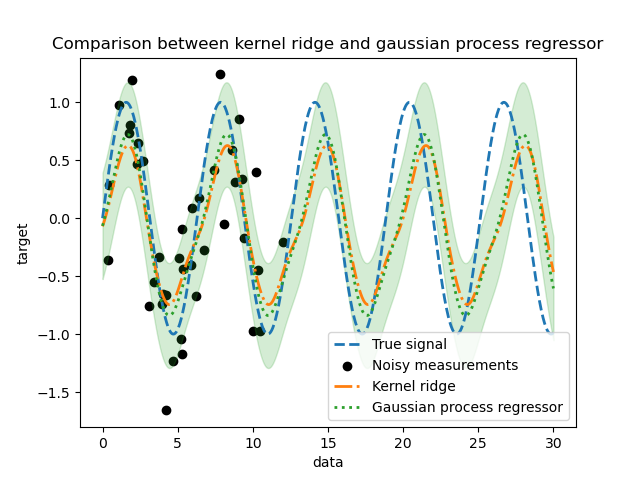
\includegraphics[width=0.9\linewidth]{fig/plot_gpr_kernel.png}
    \caption{เปรียบเทียบการเรียนรู้ Target ระหว่างเทคนิค KRR และ GPR (เครดิตภาพ: https://scikit-learn.org)}
    \label{fig:krr_gpr}
\end{figure}

ภาพที่ \ref{fig:krr_gpr} แสดงการเปรียบเทียบความแม่นยำในการทำนายค่า Target ระหว่าง KRR (เส้นสีส้ม) และ GPR (เส้นประสีเขียว) 
และมีค่าอ้างอิง (เส้นประสีฟ้า) เป็นตัวชี้วัดความแม่นยำ โดยสรุปได้ว่า GPR มีความแม่นยำและความถูกต้องในการทำนายเทียบเท่าพอ ๆ กับ KRR 
ตลอดช่วงของจำนวนข้อมูล เมื่อเราทำการเพิ่มขนาดของชุดข้อมูลจะพบว่าโมเดลทั้งสองอันจะให้ค่าที่ยังสอดคล้องกันแต่จะ Deviate ออกห่างจาก%
ค่าอ้างอิงมากขึ้นเรื่อย ๆ 

รายละเอียดของ Gaussian Process นั้นมีเยอะมาก ถ้าหากผู้อ่านสนใจศึกษาเพิ่มเติมเกี่ยวกับทฤษฎีเชิงลึกและคณิตศาสตร์ที่ใช้ในการอธิบายวิธีนี้%
ผู้เขียนแนะนำหนังสือ \textit{Gaussian Processes for Machine Learning} ของ Carl Edward Rasmussen และ 
Christopher K. I. Williams ซึ่งสามารถอ่านและดาวน์โหลดได้ฟรีที่ \url{http://gaussianprocess.org/gpml}
 % วิธีเคอร์เนล
% LaTeX source for ``การเรียนรู้ของเครื่องสำหรับเคมีควอนตัม (Machine Learning for Quantum Chemistry)''
% Copyright (c) 2022 รังสิมันต์ เกษแก้ว (Rangsiman Ketkaew).

% License: Creative Commons Attribution-NonCommercial-NoDerivatives 4.0 International (CC BY-NC-ND 4.0)
% https://creativecommons.org/licenses/by-nc-nd/4.0/

\chapter{การเรียนรู้เชิงลึก}
\label{ch:deep_learning}

ในบทนี้เราจะมาดูหัวข้อการเรียนรู้เชิงลึกหรือ Deep Learning ซึ่งเป็นหนึ่งใน Buzzword (สิ่งที่กำลังเป็นที่พูดถึงหรือได้รับความนิยม โดยที่ฟังแล้ว%
ก็อาจจะเป็นคำเก๋ ๆ) ที่หลาย ๆ คนต่างก็พูดถึงในช่วงระยะเวลา 10 ปีที่ผ่านมาโดยเฉพาะอย่างยิ่งในช่วงเวลาที่ผู้เขียนกำลังเขียนหนังสือเล่มนี้ 
ไม่ว่าจะเป็นวงการหรืออาชีพไหน ๆ ก็จะต้องมีการนำ Deep Learning เข้าไปกระยุกต์ใช้ทั้งนั้น และแน่นอนว่าหนึ่งในนั้นก็คือการนำมาประยุกต์ใช้%
ในงานวิจัยทางด้านเคมี ซึ่งข้อมูลที่นักเคมีมีอยู่ในมือนั้นมากมายมหาศาล ดังนั้นจึงน่าสนใจว่า Deep Learning จะช่วยนักเคมีในการขับเคลื่อนงาน%
วิจัยได้อย่างไร

ถ้าจะให้นิยาม Deep Learning แบบเข้าใจง่าย ๆ โดยใช้การยกตัวอย่างก็คือเป็นเทคนิคในการสร้างโมเดลคอมพิวเตอร์ที่ได้จากการฝึกฝนให้สามารถ%
ทำงานได้เหมือนมนุษย์แบบที่มีสภาวะในการทำงานที่ซับซ้อนมาก ๆ (ที่มาของคำว่าลึกหรือ Deep) เช่น การสังเกต การจดจำคำพูด การระบุภาพ 
หรือการคาดการณ์ แทนที่จะจัดระเบียบข้อมูลที่จะคำนวณผ่านทางสมการที่กำหนดไว้ล่วงหน้า Deep Learning จะกำหนดค่าพารามิเตอร์พื้นฐาน%
เริ่มต้นเกี่ยวกับข้อมูล (Hyperparameters) และฝึกให้คอมพิวเตอร์เรียนรู้ด้วยตัวเองโดยการจดจำรูปแบบโดยการใช้การประมวลผลหลายชั้น
อีกหนึ่งวัตถุประสงค์ของการพัฒนา Deep Learning นั้นก็คือการสร้าง Neural Network ที่สามารถสกัดหรือดึงสิ่งที่ซ่อนอยู่ภายในข้อมูล (Hidden 
Features) ออกมาได้ด้วยตัวของโมเดลเองโดยปราศจากการช่วยเหลือจากผู้ใช้งานหรือมนุษย์

\begin{figure}[htbp]
    \centering
    \includegraphics[width=0.7\linewidth]{fig/wisard.png}
    \caption{เครื่องการเรียนรู้เชิงลึก WISARD เครื่องแรกของโลก ณ พิพิธภัณฑ์วิทยาศาสตร์ กรุงลอนดอน ประเทศอังกฤษ 
    (เครดิตภาพ: รังสิมันต์ เกษแก้ว)}
    \label{fig:wisard}
\end{figure}

จริง ๆ แล้ว Deep Learning นั้นถือว่าเป็นอัลกอริทึมประเภทหนึ่งของ Neural Network ซึ่งเป็นเทคนิคปัญญาประดิษฐ์แบบหนึ่งที่ถูกพัฒนาขึ้นมา%
เพื่อศึกษารูปแบบที่แน่นอนของข้อมูลเรียกว่า \textit{การรับรู้รูปแบบ (Pattern Recognition)} ซึ่งเป็นกระบวนที่ทำงานเลียนแบบ (Mimic) 
สมองของมนุษย์ในการแยกแยะความจำเพาะเจาะจงบางอย่างออกมาจากข้อมูลที่ป้อนเข้าไป ภาพที่ \ref{fig:wisard} แสดงเครื่อง WISARD 
ซึ่งเป็นคอมพิวเตอร์เครื่องแรกของโลกที่ถูกสร้างขึ้นมาในปี ค.ศ. 1981 สำหรับการคำนวณ Deep Learning

ผู้เขียนขอสรุปสั้น ๆ เพื่อไม่ให้สับสนดังนี้ \textit{\enquote{Deep Learning ทุกรูปแบบเป็น Machine Learning แต่ว่าไม่ใช่ Machine 
Learning ทุกเทคนิคที่จะเป็น Deep Learning}}

ในบทก่อนหน้านี้นั้นเราได้พูดถึง Supervised Learning กันไปแล้ว ซึ่งจะเป็นการทำนายค่า $y$ จากข้อมูลนำเข้า $x$ โดยเป็นการพิจารณาใน%
กรณีของการถดถอยเชิงเส้น ในลำดับถัดมา (ซึ่งก็คือในบทนี้) เราจะมาพิจารณากรณีที่พารามิเตอร์ของเรานั้นมีความไม่เป็นเชิงเส้น (Nonlinear) 
กันครับ ซึ่งโมเดลปัญญาประดิษฐ์ที่ถูกนำมาใช้อย่างแพร่หลายนั้นก็คือ Neural Network นั่นเอง โดยเฉพาะ Deep Learning ที่ ณ ปัจจุบันได้มี%
การพัฒนาและปรับปรุงจนมีประสิทธิภาพที่สูงมาก ข้อดีอย่างหนึ่งของ Neural Network ก็คือสามารถจัดการกับข้อมูลที่มีความซับซ้อนที่มีจำนวน 
Feature หลายร้อยหรือหลายพัน Feature ได้

%--------------------------
\section{การเรียนรู้ของโมเดลที่ไม่เป็นเชิงเส้น}
\label{sec:nonlinear_ml}
\idxboth{การเรียนรู้ของโมเดลที่ไม่เป็นเชิงเส้น}{Nonlinear Supervised Learning}
%--------------------------

สมมติว่าเรามี $\{(x^{(i)}, y^{(i)})\}^n_{i=1}$ ซึ่งเป็นตัวอย่างชุดข้อมูลฝึกสอน (Training Data) และเราจะเริ่มกันด้วยกรณีที่ง่ายที่สุด%
นั่นก็คือ $y^{(i)} \in \mathbb{R}$ และ $h_\theta(x) \in \mathbb{R}$ 

เราจะทำการกำหนด Loss หรือ Coss Function ขึ้นมาก่อน ซึ่งเราจะใช้ Least Square Cost Function สำหรับข้อมูลลำดับที่ $i$ นั่นก็คือ%
คู่อันดับ $(x^{(i)} ,y^{(i)})$ ดังนี้ 

\begin{equation}\label{eq:loss}
    J^{(i)} (\theta) = \frac{1}{2} \left(h_\theta (x^{(i)}) - y^{(i)}\right)^2
\end{equation}

\noindent และกำหนด Mean-Square Cost Function สำหรับชุดข้อมูลดังนี้

\begin{equation}\label{eq:mse_loss}
    J(\theta) = \frac 1 n \sum_{i=1}^n J^{(i)}(\theta)
\end{equation}

\noindent ซึ่งผู้อ่านอาจจะสังเกตได้ว่าสมการข้างต้นนั้นจะเหมือนกับในกรณีของ Linear Regression เว้นแต่จะต่างกันตรงที่เราได้มีการเพิ่ม $1/n$
เข้าไปในด้านหน้าของ Cost Function ซึ่งเป็นการคูณ Cost Function ด้วยปริมาณสเกลาร์นั่นเอง โดยการคูณแบบนี้จะไม่ทำให้จุดต่ำสุดสัมพัทธ์ 
(Local minima) และจุดต่ำสุดสัมบูรณ์ (Global Minima) เปลี่ยนไป นอกจากนี้ผู้อ่านจะต้องทำความเข้าใจด้วยว่าการปรับค่าพารามิเตอร์ 
(Parameterization) ของ $h_\theta(x)$ นั้นจะแตกต่างจากกรณีของ Linear Regression ถึงแม้ว่าเราจะใช้ Cost Function ที่เหมือน%
กันก็ตาม 

%--------------------------
\section{การเคลื่อนลงตามความชัน}
\label{sec:gradient_descent}
\idxboth{การเคลื่อนลงตามความชัน}{Gradient Descent}
%--------------------------

หัวข้อถัดมาคือการเคลื่อนลงตามความชัน (Gradient Descent) ซึ่งเป็นเทคนิคที่สำคัญมากเพราะเป็นเทคนิคที่เรานำมาใช้ในการปรับค่าพารามิเตอร์ 
(Optimization) เพื่อลดความคลาดเคลื่อนระหว่างค่าที่ทำนายออกมากับค่าอ้างอิง ซึ่งเป็นกระบวนการสำคัญที่ทำให้เกิดการเรียนรู้ของโมเดลนั่นเอง
ซึ่ง Gradient Descent นี้เป็นเทคนิคสุดคลาสสิกที่เรานำมาใช้เพื่อหาค่าที่เหมาะสมที่สุดให้กับฟังก์ชันหนึ่ง ๆ ซึ่งใน ML นี้เราจะใช้กับ Loss หรือ 
Coss Function นั่นเอง (ผู้อ่านสามารถศึกษารายละเอียดของ Loss Function เพิ่มเติมได้ในหัวข้อที่ \ref{sec:loss_func})

\begin{figure}[htbp]
    \centering
    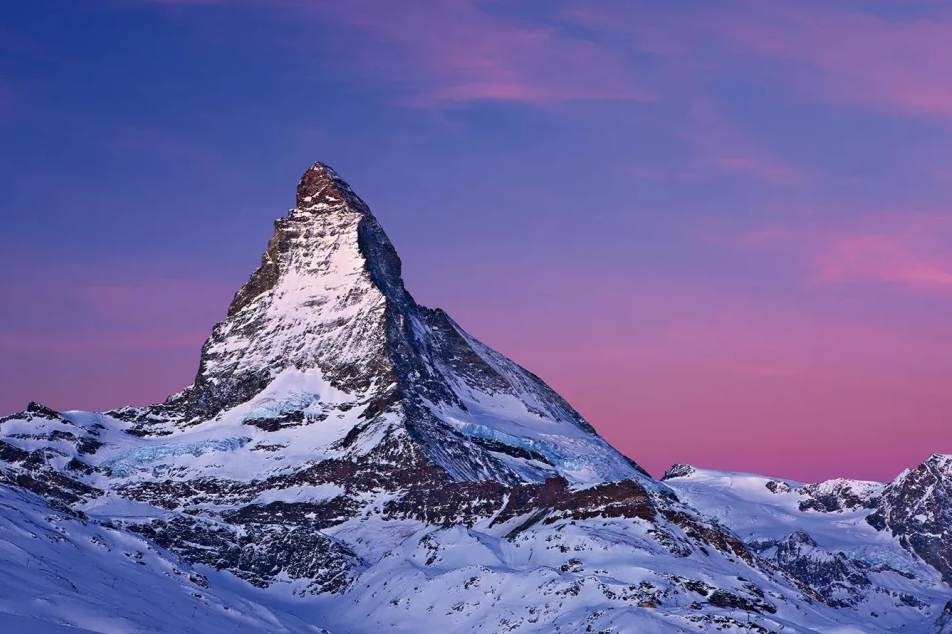
\includegraphics[width=0.8\linewidth]{fig/matterhorn.png}
    \caption{ยอดเขามัทเทอร์ฮอร์น (Matterhorn) ตั้งอยู่บนแนวของเทือกเขาแอลป์ ประเทศสวิตเซอร์แลนด์
    (เครดิตภาพ: https://www.myswitzerland.com)}
    \label{fig:matterhorn}
\end{figure}

Gradient เป็นกระบวนการทำซ้ำ (Iterative Process) โดยทําการขยับหรือกระโดดจากจุดหนึ่ง ($x^{k}$) ไปยังอีกจุดหนึ่ง ($x^{k+1}$) 
ในทิศทางที่ทําให้ค่าของฟังก์ชันมีค่าเพิ่มขึ้นหรือลดลงในปัญหาของการหาค่าสูงสุดหรือค่าต่ำสุดตามลำดับ จนกระทงได้ค่าเหมาะสมออกมา โดยสิ่งที่ 
Gradient Descent ทำในการหาพารามิเตอร์ที่เหมาะสมของฟังก์ชันก็คือการวนหาค่าที่ทำให้ Loss Function มีความคลาดเคลื่อนน้อยที่สุด 
โดยเราจะแทนความคลาดเคลื่อนหรือ Error ที่เกิดขึ้นด้วย $J$ (เช่นสมการที่ \ref{eq:loss}) หรืออธิบายง่าย ๆ ก็คือหาจุดที่มี $J$ ต่ำที่สุด%
จากการคำนวณความชัน (Slope) ณ จุดที่เราอยู่แล้วพยายามหาเส้นทางในการขยับจุดไปในทิศทางตรงข้ามกับ Slope โดยให้ลองนึกภาพว่าเรา%
กำลังเดินขึ้นเขา เช่น ตามภาพที่ \ref{fig:matterhorn} โดยวิธีการเดินเพื่อไปให้ถึงจุดสูงสุดคือเราไต่ขึ้นตามทางที่ชันขึ้นเพื่อไปถึงจุดสูงสุดนั่นเอง 
ถ้ายิ่งชันเท่าไหร่ก็มีแนวโน้มว่าเราเข้าใกล้จุดสูงสุดมากขึ้นเท่านั้น

Gradient Descent เป็นอัลกอริทึมที่ใช้หาจุดต่ำสุดหรือสูงสุดของฟังก์ชันซึ่งโดยส่วนมากเป็นฟังก์ชันรูปกรวยคว่ำ (Convex) แต่ถ้าลองดูตัวอย่างง่าย ๆ
เช่น ฟังก์ชันพาราโบลาหงายที่มีฟังก์ชันเป็น 

\begin{equation}\label{eq:parabola}
    f(x) = x^2 - 4x
\end{equation}

\noindent เราจะสามารถหาอนุพันธ์ของสมการที่ \ref{eq:parabola} ได้ง่าย ๆ ซึ่งจะได้ออกมาเป็นสมการที่อธิบายความชัน ดังนี้

\begin{align}\label{eq:eq:parabola_slope}
    f'(x) &= \nabla f(x) \nonumber \\
    &= 2x - 4
\end{align}

%--------------------------
\subsection{Batch Gradient Descent}
\label{ssec:batch_grad}
\idxth{การเคลื่อนลงตามความชัน!แบทช์}
\idxen{Gradient Descent!Batch}
%--------------------------

คราวนี้เราลองมาดูกรณีที่ Loss Function นั้นเป็นแบบกรณีทั่วไปกันบ้าง โดยเรานิยามให้ Loss Function มีหน้าตาแบบนี้

\begin{align}
    J(\theta) &= J(\theta_0, \theta_1) \nonumber \\
    &= \cfrac{1}{2m} \sum_{i=1}^m ((\theta_0 + \theta_1 x^{(i)}) - y^{(i)})^2
\end{align}

\noindent เราสามารถหา Gradient ได้ดังนี้

\begin{align}
    \nabla J (\theta) &= \begin{bmatrix} \cfrac{\partial J}{\partial \theta_0}\\ \cfrac{\partial J}{\partial 
    \theta_1} \end{bmatrix} \\
    &=  \begin{bmatrix} \frac{1}{m} \sum_{i=1}^{m} ((\theta_0 + \theta_1 x^{(i)}) - y^{(i)}) \\ \frac{1}{m} 
    \sum_{i=1}^{m} ((\theta_0 + \theta_1 x^{(i)}) - y^{(i)})x^{(i)} \end{bmatrix}
\end{align}

\noindent ซึ่งเราสามารถเขียนสมการในกรณีที่เราสนใจและอัพเดท $\theta$ ได้ดังนี้\footnote{สังเกตว่าเราใช้เครื่องหมาย $a := b$ 
เพื่อบ่งบอกการดำเนินการ (Operation) ซึ่งเป็นการระบุค่าให้กับตัวแปรในโปรแกรมคอมพิวเตอร์}

\begin{equation}\label{eq:batch_grad}
    \theta := \theta - \alpha\nabla_\theta J(\theta)
\end{equation}

\noindent โดยสมการที่ \ref{eq:batch_grad} นั้นคือ Batch Gradient Descent มีสัมประสิทธิ์ด้านหน้า $\nabla_\theta J$ ก็คือ 
$\alpha$ คืออัตราเร็วในการเรียนรู้ \textit{Learning Rate} หรืออาจจะเรียกว่า \textit{Step Size} ก็ได้ โดยเรามักจะกำหนดให้ค่า 
$\alpha$ มีค่ามากกว่าศูนย์ ซึ่งเป็นอัลกอริทึมแบบที่ง่ายที่สุดเพราะว่าใช้ข้อมูลทั้งหมดใน Training Set ในการฝึกสอนโมเดล ดังนั้นผู้อ่านน่าจะ%
พอเดาออกว่าถ้าหากเราใช้ Batch Gradient Descent กับชุดข้อมูลที่มีขนาดใหญ่มากนั้นก็จะใช้ระยะเวลานานในการฝึกสอนโมเดล นั่นก็เพราะว่า 
Optimization แบบ Batch นั้นช้ามาก ด้านล่างคืออัลกอริทึมของ Batch Gradient Descent

\begin{algorithm}[H]
    \caption{อัลกอริทึมของ Batch Gradient Descent}
    \label{alg:batch_grad}
    \begin{algorithmic}
    \State Hyperparameter: learning rate $\alpha$, number of total iteration $n_\text{iter}$.
    \State Initialize $\theta$ randomly.
    \For{$i = 1$ to $n_\text{iter}$}
        \begin{equation*}
            \theta := \theta - \alpha\nabla_\theta J^{(j)}(\theta)
        \end{equation*}
    \EndFor
    \end{algorithmic}
\end{algorithm}

\noindent ตัวอย่างของโค้ดของ Batch Gradient Descent มีดังนี้

\begin{lstlisting}[style=MyPython]
for i in range(nb_epochs):
    params_grad = evaluate_gradient(loss_function, data, params)
    params = params - learning_rate * params_grad
\end{lstlisting}

%--------------------------
\subsection{Stochastic Gradient Descent}
\label{ssec:stochastic_grad}
\idxth{การเคลื่อนลงตามความชัน!สโตแคสติก}
\idxen{Gradient Descent!Stochastic}
%--------------------------

เพื่อแก้ปัญหาในกรณีที่ชุดข้อมูลมีขนาดใหญ่มากนั้น จึงได้มีการพัฒนาอัลกอริทึมแบบที่สองขึ้นมา เรียกว่า Stochastic Gradient Descent (SGD) 
โดย SGD นี้เป็นวิธีที่ง่ายและไม่ซับซ้อนในการนำมาใช้ปรับค่าพารามิเตอร์ให้มีความเหมาะสม โดยในแต่ละครั้งของการคำนวณ Gradient เราจะทำ%
การสุ่มข้อมูลเพียงบางส่วนเพื่อใช้ในการอัพเดทค่าเท่านั้น ไม่ได้ใช้ข้อมูลทั้งหมดเหมือนในกรณี Batch โดยตามทฤษฎีแล้วได้มีการพิสูจน์ว่าเรา%
สามารถใช้ข้อมูลในปริมาณที่เล็กน้อยเพื่อใช้ในการอัพเดทพารามิเตอร์ในแต่ละครั้ง (Iteration) ได้โดยไม่ต้องนำข้อมูลทั้งหมดมาใช้ทีเดียว 
ซึ่งในท้ายที่สุดแล้วการ Optimization ก็จะลู่เข้าสู่คำตอบที่ใกล้เคียงกัน ซึ่ง SGD นี้ถือว่ามีส่วนสำคัญต่อการฝึกสอนโมเดลที่มีพารามิเตอร์ที่เกี่ยวข้อง%
ในปริมาณที่เยอะมาก ๆ เช่น Neural Network การใช้ SGD สามารถลดปัญหาของการที่ Optimization นั้นติดหรือค้างอยู่ในจุดต่ำสุดสัมพันธ์%
ได้อีกด้วย ซึ่งการปรับค่าด้วย SGD นั้นจะใช้สมการดังต่อไปนี้

\begin{equation}\label{eq:sgd}
    \theta := \theta - \alpha\nabla_\theta J( \theta; x^{(i)}; y^{(i)})
\end{equation}

\noindent ด้านล่างคืออัลกอริทึมของ SGD

\begin{algorithm}[H]
    \caption{อัลกอริทึมของ Stochastic Gradient Descent}
    \label{alg:sgd}
    \begin{algorithmic}
    \State Hyperparameter: learning rate $\alpha$, number of total iteration $n_\text{iter}$.
    \State Initialize $\theta$ randomly.
    \For{$i = 1$ to $n_\text{iter}$}
        \State Sample $j$ uniformly from ${1,\ldots,n}$, and update $\theta$ by
        \begin{equation*}
            \theta := \theta - \alpha\nabla_\theta J^{(j)}(\theta)
        \end{equation*}
    \EndFor
    \end{algorithmic}
\end{algorithm}

\noindent ตัวอย่างของโค้ดของ Stochastic Gradient Descent มีดังนี้

\begin{lstlisting}[style=MyPython]
for i in range(nb_epochs):
    np.random.shuffle(data)
    for example in data:
        params_grad = evaluate_gradient(loss_function, example, params)
        params = params - learning_rate * params_grad
\end{lstlisting}

\noindent นอกจากนี้แล้วในการฝึกสอนโมเดล Neural Network นั้น เรามักนิยมใช้ Stochastic Gradient Descent โดยด้านล่างคือ%
ตัวอย่างโค้ดของการเรียกใช้ Stochastic Gradient Descent (SGD) Optimizer ของ TensorFlow

\begin{lstlisting}[style=MyPython]
# Create an optimizer with the desired parameters.
opt = tf.keras.optimizers.SGD(
    learning_rate=0.01,
    momentum=0.0,
    nesterov=False,
    name='SGD',
    **kwargs
)

# `loss` is a callable that takes no argument and returns the value
# to minimize.
loss = lambda: 3 * var1 * var1 + 2 * var2 * var2

# In graph mode, returns op that minimizes the loss by updating the listed
# variables.
opt_op = opt.minimize(loss, var_list=[var1, var2])
opt_op.run()

# In eager mode, simply call minimize to update the list of variables.
opt.minimize(loss, var_list=[var1, var2])
\end{lstlisting}

%--------------------------
\subsection{Mini-batch Stochastic Gradient Descent}
\label{ssec:minibatch_grad}
\idxth{การเคลื่อนลงตามความชัน!มินิ-แบทช์}
\idxen{Gradient Descent!Mini-batch}
%--------------------------

นอกเหนือจาก Batch และ Stochastic Gradient Descent แล้ว ยังมีอัลกอริทึมแบบที่สามที่เป็นการรวมข้อดีของทั้งสองอัลกอริทึมเข้าไว้ด้วยกัน
นั่นคืออัลกอริทึมที่ชื่อว่า Mini-batch Stochastic Gradient Descent โดยแรสคิดก็คือในทางปฏิบัตินั้นการคำนวณ Gradient ของ Batch 
($B$) หลาย ๆ ครั้งสามารถทำพร้อมกันได้เพราะว่าในปัจจุบันเรามีเทคนิคการทำการคำนวณแบบขนาน (Parallelization) สำหรับการปรับค่า 
$\theta$ ซึ่งจะเร็วกว่าการคำนวณ Gradient ของ $B$ แบบแยกกันทีละค่าแน่นอน ซึ่งการที่เราจะทำการคำนวณแบบพร้อม ๆ กันได้นั้นเราจะ%
ต้องมีการแบ่งข้อมูลของเราออกเป็นส่วนย่อย ๆ แล้วทำการคำนวณแยกกัน โดยมีสมการดังต่อไปนี้ 

\begin{equation}\label{eq:minibatch}
    \theta = \theta - \alpha\nabla_\theta J( \theta; x^{(i:i+n)}; y^{(i:i+n)})
\end{equation}

ในการคำนวณจริงนั้นเราจะต้องมีการปรับอัลกอริทึมเล็กน้อย โดยด้านล่างคืออัลกอริทึมของ Mini-batch SGD ซึ่งได้จากการปรับอัลกอริทึมของ SGD 
แบบธรรมดา

\begin{algorithm}[H]
    \caption{อัลกอริทึมของ Mini-batch Stochastic Gradient Descent}
    \label{alg:minibatch}
    \begin{algorithmic}
    \State Hyperparameter: learning rate $\alpha$, batch size $B$, \# iteration $n_\text{iter}$.
    \State Initialize $\theta$ randomly.
    \For{$i = 1$ to $n_\text{iter}$}
        \State Sample $j$ uniformly from ${1,\ldots,n}$, and update $\theta$ by
        \State Sample $B$ examples $j_1,\ldots,j_B$ (without replacement) uniformly from $\{1,\ldots,n\}$, 
        and update $\theta$ by
        \begin{equation*}
            \theta := \theta - \frac{\alpha}{B}\sum_{k=1}^B\nabla_\theta J^{(j_k)}(\theta)
        \end{equation*}
    \EndFor
    \end{algorithmic}
\end{algorithm}

\noindent ตัวอย่างของโค้ดของ Mini-batch Stochastic Gradient Descent มีดังนี้

\begin{lstlisting}[style=MyPython]
for i in range(nb_epochs):
    np.random.shuffle(data)
    for batch in get_batches(data, batch_size=50):
        params_grad = evaluate_gradient(loss_function, batch, params)
        params = params - learning_rate * params_grad
\end{lstlisting}

\noindent $\bullet$ \textbf{สรุปเปรียบเทียบอัลกอริทึมของ Gradient Descent}

\begin{figure}[htbp]
    \centering
    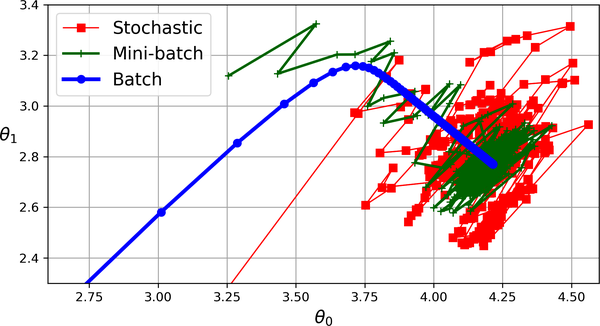
\includegraphics[width=0.9\linewidth]{fig/gradient_descent_path.png}
    \caption{วิถีของ Gradient Descent ในปริภูมิของพารามิเตอร์ (เครดิตภาพ: https://www.oreilly.com)}
    \label{fig:gradient_descent_path}
\end{figure}

ภาพที่ \ref{fig:gradient_descent_path} แสดงการเปรียบเทียบวิถี (Path) ของการขยับของ Gradient Descent ด้วยอัลกอริทึมที่ต่างกัน
ซึ่งแสดงอยู่บนปริภูมิพารามิเตอร์ โดยสรุปได้ว่าทั้งสามอัลกอริทึมนั้นให้ผลลัพธ์ที่เข้าใกล้จุดต่ำสุดแต่ว่าจริง ๆ แล้ว Batch Gradient Descent 
นั้นหยุดอยู่ที่จุดต่ำสุดพอดีในขณะที่ Stochastic และ Mini-batch Gradient Descent นั้นจะขยับวนไปมาอยู่รอบ ๆ จุดต่ำสุดและยังคงขยับ%
ไปมาอยู่เรื่อย ๆ อย่างไรก็ตามเราจะต้องไม่ลืมว่าอัลกอริทึมแบบ Batch นั้นใช้ระยะเวลาในการขยับจากจุดหนึ่งไปยังอีกจุดหนึ่งที่นานมาก แต่อีกสอง%
อัลกอริทึมนั้นใช้เวลาน้อยกว่ามาก ซึ่งถ้าหากเราเลือกใช้อัลกอริทึม Stochastic หรือ Mini-batch ได้อย่างเหมาะสมแล้วทั้งสองอัลกอริทึมนี้ก็%
สามารถให้ผลลัพธ์ที่ลู่เข้า (Convergence) สู่จุดต่ำสุดได้เช่นเดียวกัน

โดยทั่วไปแล้วโมเดล Deep Learning นั้นจะมีการเรียนรู้ซึ่งอาศัยอัลกอริทึมตามด้านบนโดยทำตามขั้นตอนดังต่อไปนี้

\begin{enumerate}[topsep=0pt,noitemsep]
    \item กำหนด $h_\theta(x)$
    
    \item เขียนอัลกอริทึม Backpropagation เพื่อคำนวณ Gradient ของ Loss Function $J^{(j)}(\theta)$
    
    \item ทำการปรับ Loss Function โดยใช้ SGD หรือ Mini-batch SGD หรือใช้อัลกอริทึมอื่น เช่น Normal Equation หรือ SVD
\end{enumerate}

นอกจากนี้แล้วอีกสิ่งหนึ่งที่เราต้องคำนึงถึงก็คือ Learning Rate ซึ่งเป็นค่าอัตราเร็วของการเรียนรู้ โดยพารามิเตอร์ตัวนี้มีผลทั้งในเชิงประสิทธิภาพ%
ของอัลกอริทึมที่ใช้ในการปรับให้การ Optimization นั้นลู่เข้าและมีผลต่อความเร็วหรือความสิ้นเปลืองในการปรับค่าด้วย

\begin{figure}[htbp]
    \centering
    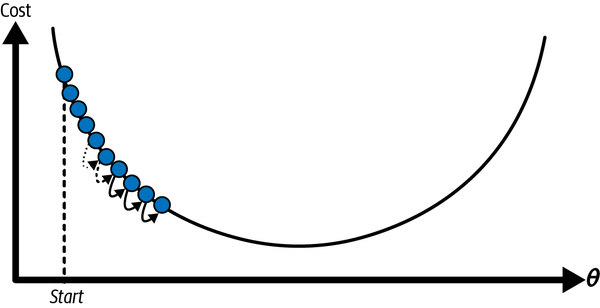
\includegraphics[width=0.8\linewidth]{fig/learning_rate_small.png}
    \caption{แสดงค่าคลาดเคลื่อน (Error หรือ Cost) เทียบกับการเปลี่ยนแปลงของการเรียนรู้ในกรณีที่กำหนดให้ Learning Rate นั้นมี%
    ที่น้อยมาก ๆ (เครดิตภาพ: https://www.oreilly.com)}
    \label{fig:learning_rate_small}
\end{figure}

\begin{figure}[htbp]
    \centering
    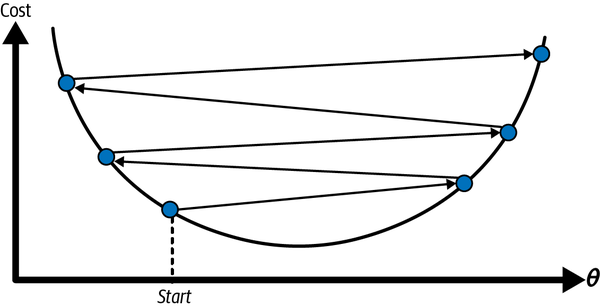
\includegraphics[width=0.8\linewidth]{fig/learning_rate_high.png}
    \caption{แสดงค่าคลาดเคลื่อน (Error หรือ Cost) เทียบกับการเปลี่ยนแปลงของการเรียนรู้ในกรณีที่กำหนดให้ Learning Rate นั้นมี%
    ที่สูงมาก ๆ (เครดิตภาพ: https://www.oreilly.com)}
    \label{fig:learning_rate_high}
\end{figure}

ภาพที่ \ref{fig:learning_rate_small} และ \ref{fig:learning_rate_high} แสดงความสามารถในการขยับหรือปรับค่าของการทำ 
Gradient Descent จากจุดหนึ่งไปยังอีกจุดหนึ่งโดยใช้อัตราเร็วในการเรียนรู้ที่มีค่าน้อย ๆ และค่าสูง ๆ ตามลำดับ โดยเราสามารถสรุปได้ว่าในกรณี%
ที่เราใช้อัตราการเรียนรู้ที่มีค่าน้อยเกินไปนั้นจะเป็นการขยับจุดแบบช้ามาก ๆ และการขยับไปในแต่ละจุดนั้นจะเป็นแบบก้าวสั้น ๆ แต่ก็ให้ผลลัพธ์ที่มีความ%
แม่นยำและค่อย ๆ ขยับจุดเข้าไปใกล้จุดต่ำสุดตามที่ต้องการ ซึ่งจะตรงข้ามกับกรณีที่ใช้อัตราการเรียนรู้ที่สูงเกินไปนั่นก็คือการขยับจุดนั้นเป็นไปอย่าง%
รวดเร็ว และระยะห่างระหว่างจุดหรือขนาดของก้าวแต่ละก้าวนั้นจะกว้างกว่ามาก แต่จะพบว่าการปรับค่าเข้าไปหาจุดต่ำสุดนั้นจะทำได้ไม่ค่อยดีเพราะจะ%
เป็นการขยับจุดที่เร็วเกินไปทำให้เกิดการวนซ้ำไปซ้ำมารอบ ๆ จุดต่ำสุดและทำให้ลู่เข้าได้ยาก

สรุปคือเราควรจะต้องกำหนดอัตราเร็วของการเรียนรู้ให้มีความเหมาะสม ถ้าหากอัตราการเรียนรู้ช้าเกินไปก็จะใช้เวลานาน แต่ถ้าหากอัตราการเรียนรู้เร็ว%
เกินไปก็จะทำให้การปรับค่านั้นได้ผลลัพธ์ที่ไม่แม่นยำ

%--------------------------
\section{โครงข่ายประสาทเทียม}
\label{sec:nn}
\idxboth{โครงข่ายประสาทเทียม}{Neural Network}
\idxen{Artificial Neural Network}
%--------------------------

โครงข่ายประสาทเทียม (Neural Network) ถือว่าเป็นโมเดล ML แบบหนึ่งที่มีประสิทธิภาพสูงมากและเป็นสิ่งที่พลิกโฉมหน้าประวัติศาสตร์ของวงการ%
ปัญญาประดิษฐ์เลยก็ว่าได้ ตามที่ได้อธิบายไว้คร่าว ๆ ในหัวข้อ \ref{ssec:ann} แล้วว่า Neural Network นั้นเป็นการเลียนแบบการทำงานของ%
สมองมนุษย์ ซึ่งในช่วงยุคต้นของการพัฒนาเทคนิคนี้นั้นมีจุดประสงค์คือการแก้ปัญหาแบบเดียวกับที่สมองมนุษย์สามารถทำได้ แต่เมื่อเวลาผ่านไป%
จุดประสงค์ของการสร้าง Neural Network ก็ได้เปลี่ยนไปเป็นการทำงานที่เฉพาะเจาะจงมากขึ้น และมีการพัฒนาให้สามารถทำงานหรือแก้ปัญหาให้%
ดีกว่ามนุษย์เสียอีก ซึ่งเป็นการแทนจุดประสงค์เดิมในการสร้างสมองเทียม โดยในปัจจุบันมีการประยุกต์ใช้โ Neural Network กับงานหลากหลายรูปแบบ 
เช่น คอมพิวเตอร์วิทัศน์ (Computer Vision), การเรียนรู้เสียง (Voice Learning และ Recognition), การแปลภาษา (Translation), 
การกรองเนื้อหาโซเชียลมีเดีย, การเล่นเกม, การวินิจฉัยโรค และกิจกรรมที่ไม่คิดว่าปัญญาประดิษฐ์จะทำได้ เช่น การวาดภาพ, การประพันธ์เพลง 
และการประพันธ์บทกวี

Neural Network ที่พบได้ทั่วไปจะมีลักษณะคือประกอบไปด้วยชั้นของเซล์ประสาทเทียม (Layer) ชั้นที่รับข้อมูลขาเข้าเรียกว่าชั้นอินพุต (Input 
Layer) ชั้นที่สร้างข้อมูลขาออกหรือเอาต์พุต (Output Layer) ส่วนชั้นอื่น ๆ ที่มีส่วนในการช่วยทำการประมวลผลอยู่ภายในเรียกว่าชั้นซ่อน 
(Hidden Layer) ซึ่งใน Neural Network อาจมี Hidden Layer ได้หลายชั้น นอกจากนี้เราสามารถแบ่งโครงสร้างพื้นฐานตามการไหล (Flow) 
ของข้อมูลได้ดังต่อไปนี้

\begin{itemize}
    \item แบบป้อนไปข้างหน้า (Feed Forward) เป็น Neural Network ที่ข้อมูลจะมีการไหลหรือส่งต่อไปในทิศทางเดียวจาก Input Layer 
    ไปยัง Hidden Layer และ Output Layer ตามลำดับ การเชื่อมโยงจะถูกกำหนดขึ้นระหว่างชั้นที่ติดกันโดยจะมีการเชื่อมโยงระหว่างเซลล์%
    ประสาทเทียม (Neuron) ทุกตัว จากชั้นหนึ่ง ๆ ไปยังเซลล์ประสาทเทียมทุกตัวในชั้นต่อไป ในบางสถาปัตยกรรมอาจมีการเชื่อมโยงข้ามชั้นก็ได้ 
    นอกจากนี้แล้วรูปแบบของ Neural Network ประเภทนี้ยังจัดแบ่งได้เป็นสองแบบย่อยคือ แบบมีชั้นของเซลล์ประสาทชั้นเดียว และแบบมีชั้น%
    ของเซลล์ประสาทหลายชั้น 

    \item แบบมีการป้อนไปเวียนกลับ (Recurrent) เป็น Neural Network ที่การเชื่อมโยงที่ถูกกำหนดขึ้นระหว่างเซลล์ประสาทเทียมในชั้น%
    หนึ่ง ๆ นั้นย้อนกลับไปยังชั้นอื่น ๆ ก่อนหน้านั้นได้หรือแม้แต่ภายในชั้นเดียวกันเองโดยผ่านการวนลูปรอบ ๆ เซลล์ประสาทนั้น ๆ โดยการไหล%
    ของข้อมูลนั้นสามารถเกิดได้สองทิศทาง ทั้งทิศทางที่ไปข้างหน้าและย้อนกลับ สถาปัตยกรรมแบบนี้ยังมีชื่อเรียกอีกชื่อว่า Feedback Neural 
    Network
\end{itemize}

สำหรับในหัวข้อนี้เราจะมาดูการเรียนรู้เชิงลึก (Deep Learning) รูปแบบที่มาตรฐานที่สุดคือการเรียนรู้แบบมีผู้สอนด้วยโมเดลแบบไม่เป็นเชิงเส้น 
(Supervised Learning with Nonlinear Model) นอกจากนี้ Neural Network ยังมีสถาปัตยกรรมที่หลากหลายซึ่งผู้อ่านสามารถศึกษาได้%
ในหัวข้อที่ \ref{sec:arch_nn}

%--------------------------
\section{การแผ่กระจายการเรียนรู้}
\idxboth{การแผ่กระจายการเรียนรู้}{Learning Propagation}
%--------------------------

การแผ่กระจายการเรียนรู้ (Learning Propagation) เป็นขั้นตอนการเรียนรู้ของโมเดล Neural Network ที่เลียนแบบการทำงานของสมอง 

\begin{figure}[htbp]
    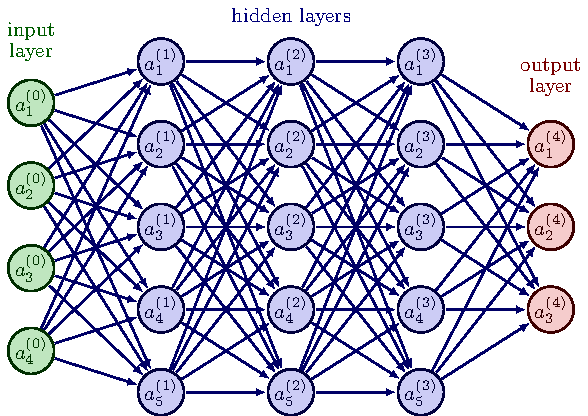
\includegraphics[width=\linewidth]{fig/dense_neural_net.pdf}
    \caption{โครงข่ายประสาทแบบสมบูรณ์ (Dense Neural Network) มี Notation $a^{(j)}_{i}$ แทนข้อมูลของหน่วยเรียนรู้หรือ%
    นิวรอนที่ $i$ ของชั้นที่ $j$ โดยชั้นที่ 1 กับชั้นที่ 4 ของตัวอย่าง Neural Network นี้คือชั้นอินพุตและชั้นเอาต์พุตตามลำดับ}
    \label{fig:dense_neural_net}
\end{figure}

จะเห็นได้ว่าไดอะแกรมด้านบนนั้นมีความซับซ้อนมาก ซึ่งจริง ๆ แล้วถ้าหากเราจะมาทำความเข้าใจองค์ประกอบของ Neural Network นั้น เราควร%
พิจารณากรณีง่าย ๆ ด้วยโครงสร้างแบบเล็ก ๆ ก่อน ตามภาพที่ \ref{fig:nn_layer} ซึ่งเป็นชั้นการเรียนรู้ (Learning Layer) ประกอบไปด้วย
3 ส่วน ดังนี้

\begin{description}
    \item[Input Layer] ชั้นอินพุต เก็บข้อมูลที่เราจะนำมาใช้ในการฝึกสอนโมเดล โดยในแต่ละหน่วยประสาท (Neuron หรือ Learning Unit 
    หรือ Node) จะเป็นตัวที่เก็บคุณลักษณ์ที่อยู่ในข้อมูล เช่น ความยาวพันธะหรือจำนวนเวเลนซ์อิเล็กตรอนของอะตอม
    
    \item[Hidden Layer] ชั้นที่ถูกซ่อนไว้ เป็นชั้นที่อยู่ระหว่างชั้นอินพุตและชั้นเอาต์พุต โดยข้อมูลที่ถูกส่งมาจากชั้นก่อนหน้า (ในที่นี้คือชั้นอินพุต)
    จะถูกนำไปผ่านฟังก์ชันกระตุ้น (Activation Function) ในชั้นนี้ และหลังจากนั้นจะถูกส่งออกไปชั้นต่อไป (ในที่นี้คือชั้นเอาต์พุต)
    
    \item[Output Layer] ชั้นเอาต์พุต เป็นชั้นสุดท้ายของ Neural Network โดยจะรับข้อมูลหรืออินพุตมาจากชั้นก่อนหน้าซึ่งเป็น Hidden 
    Layer โดยในชั้นนี้อาจจะมีการนำฟังก์ชันกระตุ้นมาใช้หรือไม่ใช้ก็ได้
\end{description}

\begin{figure}[htbp]
    \centering
    \begin{subfigure}{0.5\textwidth}
        \centering
        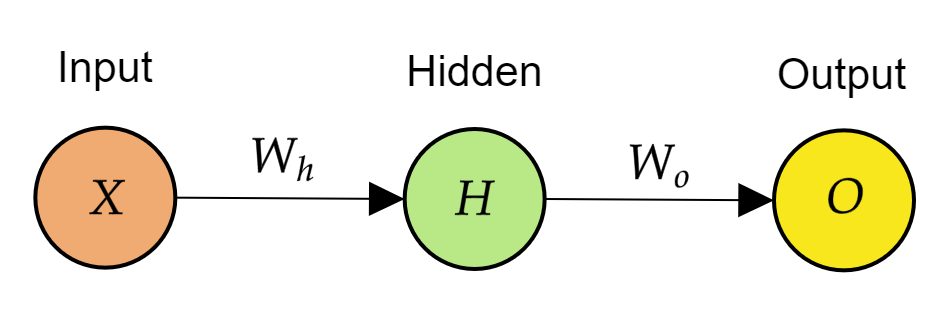
\includegraphics[width=0.9\linewidth]{fig/nn_layer.png}
        \caption{ชั้นการเรียนรู้ (Learning Layer)}
        \label{fig:nn_layer}
    \end{subfigure}%
    \begin{subfigure}{0.5\textwidth}
        \centering
        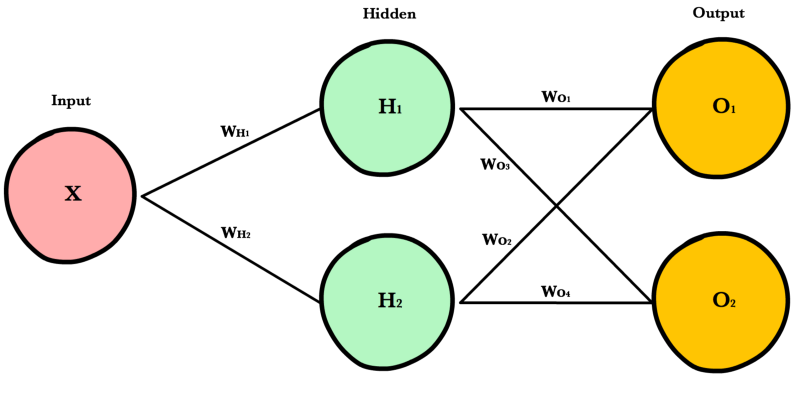
\includegraphics[width=0.9\linewidth]{fig/nn_w_matrices.png}
        \caption{โครงข่ายแบบค่าน้ำหนักหลายตัว}
        \label{fig:nn_w_matrices}
    \end{subfigure}
    \caption{ตัวอย่างของโครงข่ายประสาทแบบง่าย}
    \label{fig:nn_layer_w}
\end{figure}

โดยเราสามารถใช้โค้ดต่อไปนี้ในการสร้าง Neural Network แบบง่าย ๆ ได้

\begin{lstlisting}[style=MyPython]
def relu(z):
    return max(0,z)

def feed_forward(x, Wh, Wo):
    # Hidden layer
    Zh = x * Wh
    H = relu(Zh)

    # Output layer
    Zo = H * Wo
    output = relu(Zo)
    return output
\end{lstlisting}

เมื่อเราพิจารณาภาพที่ \ref{fig:nn_w_matrices} ซึ่งมีความซับซ้อนมากขึ้นโดยมีการเพิ่มจำนวน Neuron เข้าไปในชั้น Hidden Layer และ 
Output Layer เราจะพบว่าค่าน้ำหนักที่ถูกคำนวณออกมาจากชั้น Input จะถูกส่งไปยังชั้น Hidden และค่าน้ำหนักที่ออกมาจากชั้น Hidden ก็ถูก%
ส่งต่อไปยังชั้น Output ตามลำดับ โดยจะเห็นว่าทุก ๆ Neuron ของชั้นที่ถูกติดกันนั้นจะมีการแลกเปลี่ยนกันทุก Neuron โดยสมการที่ใช้ในการคำนวณ%
หาเอาต์พุตของแต่ละ Neuron มีดังนี้

\noindent $\bullet$ อินพุต 1 ตัว
\begin{align}\label{eq:nn_one_input}
    Z &= Input \cdot Weight \nonumber \\
    &= X W
\end{align}

\noindent $\bullet$ อินพุตมากกว่า 1 ตัว
\begin{align}\label{eq:nn_multi_input}
    Z &= \sum_{i=1}^{n}x_i w_i \nonumber \\
    &= x_1 w_1 + x_2 w_2 + x_3 w_3
\end{align}

เราจะสังเกตได้ว่าสมการที่ \ref{eq:nn_one_input} และ \ref{eq:nn_multi_input} เป็นสมการที่เหมือนกับที่เราใช้ใน Linear 
Regression เป๊ะ ๆ เลย ซึ่งจริง ๆ แล้ว Neural Network ที่มีจำนวน Neuron แค่ 1 อันนั้นคือ Linear Regression เลย แต่สิ่งที่ต่างกันก็คือ
Neural Network จะมีกระบวนที่เกี่ยวข้องกับค่าน้ำหนักและฟังก์ชันกระตุ้นด้วย สำหรับการกำหนดค่าน้ำหนักในช่วงเริ่มต้นของการฝึกสอนนั้นเราสามารถ%
กำหนดค่าได้โดยใช้การสุ่มค่าตามตัวอย่างโค้ดดังต่อไปนี้

\begin{lstlisting}[style=MyPython]
INPUT_LAYER = 1
HIDDEN_LAYER = 2
OUTPUT_LAYER = 2

def init_weights():
    Wh = np.random.randn(INPUT_LAYER, HIDDEN_LAYER) \
            * np.sqrt(2.0/INPUT_LAYER)
    Wo = np.random.randn(HIDDEN_LAYER, OUTPUT_LAYER) \
            * np.sqrt(2.0/HIDDEN_LAYER)
\end{lstlisting}

\noindent และเรามักจะกำหนดค่าเริ่มต้นของความโน้มเอียง (Bias) ด้วยค่าน้อย ๆ เช่น 0.1 หรือ 0.2 ดังตัวอย่างต่อไปนี้

\begin{lstlisting}[style=MyPython]
def init_bias():
    Bh = np.full((1, HIDDEN_LAYER), 0.1)
    Bo = np.full((1, OUTPUT_LAYER), 0.1)
    return Bh, Bo
\end{lstlisting}

%--------------------------
\subsection{การแผ่กระจายแบบไปข้างหน้า}
\label{ssec:forward_prop}
\idxboth{การแผ่กระจายการเรียนรู้!การแผ่กระจายแบบไปข้างหน้า}{Propagation!Forward Propagation}
%--------------------------

ในขั้นเริ่มต้นของการฝึกสอนโมเดล Neural Network นั้น โมเดลจะยังไม่มีพารามิเตอร์ที่ถูกต้อง ดังนั้นเราจึงต้องสุ่มค่าเริ่มต้นของพารามิเตอร์ขึ้นมาก่อน
หลังจากนั้นจึงทำ Forward Propagation รอบที่หนึ่งแล้วก็เปรียบเทียบผลการทำนายกับคำตอบ (Output) ที่โมเดลทราบก่อนหน้านั้นแล้ว
ขั้นตอนต่อมาคือการปรับพารามิเตอร์ที่สำคัญอีกสองตัวนั่นคือน้ำหนัก (Weight) และความอคติหรือความโน้มเอียง (Bias) ให้มีค่าที่ถูกต้อง 
ซึ่งในขั้นตอนนี้เราจะใช้กระบวนการที่ตรงข้ามกันที่เรียกว่า Backward propagation (หรือ Backpropagation) โดยการทำ Propagation 
ทั้งสองแบบพร้อม ๆ กันครบหนึ่งรอบนั้นจะเรียกว่า 1 Epoch แต่ต้องระวังนะครับว่า Epoch, Batch Size และ Iteration นั้นมีความหมายต่างกัน 
โดยความแตกต่างมีดังนี้

\begin{description}[font=$\bullet$~\normalfont\scshape\bfseries\color{red!50!black}]
    \item[1 Epoch] การทำ Forward และ Backward Propagation 1 ครั้ง
    
    \item[Batch Size] จำนวนของข้อมูลที่ใช้ในการฝึกสอนในการทำ Forward และ Backward Propagation 1 รอบ
    
    \item[Iteration] จำนวนของรอบในการฝึกสอน ซึ่งแต่ละรอบจะใช้ Batch Size ที่ถูกกำหนดไว้ก่อนการฝึกสอน
\end{description}

เพื่อให้เห็นภาพมากขึ้น เราลองมาดูตัวอย่างกันครับ เช่น ถ้าเรามีจำนวนข้อมูลในการฝึกสอน 1,000 ข้อมูลและกำหนด Batch Size เป็น 500 
จะได้ว่าโมเดลของเราจะใช้ 2 Iterations สำหรับการฝึกสอน 1 Epoch

\begin{figure}[htbp]
    \centering
    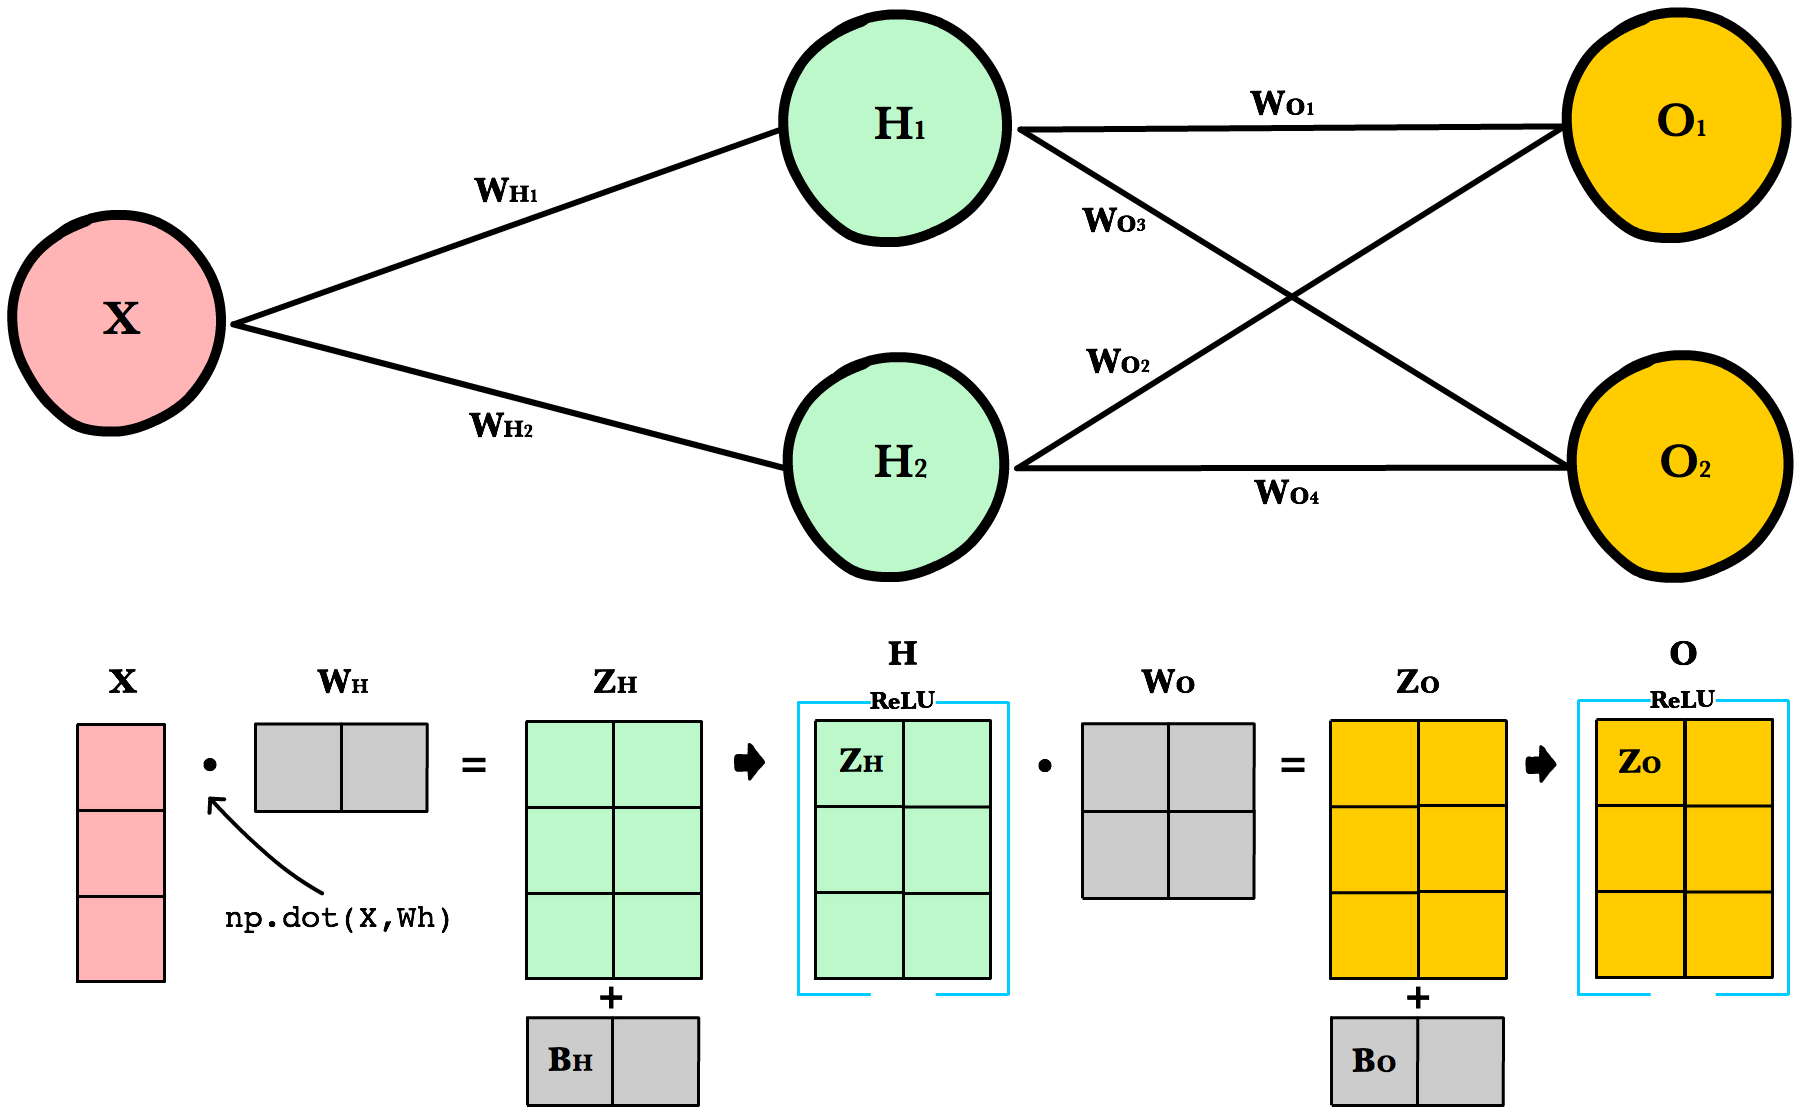
\includegraphics[width=0.9\linewidth]{fig/nn_feedforward_matrices.png}
    \caption{แผนภาพการดำเนินการคูณเมทริกซ์อินพุนด้วยเมทริกซ์น้ำหนัก}
    \label{fig:nn_ff_mat}
\end{figure}

\begin{figure}[htbp]
    \centering
    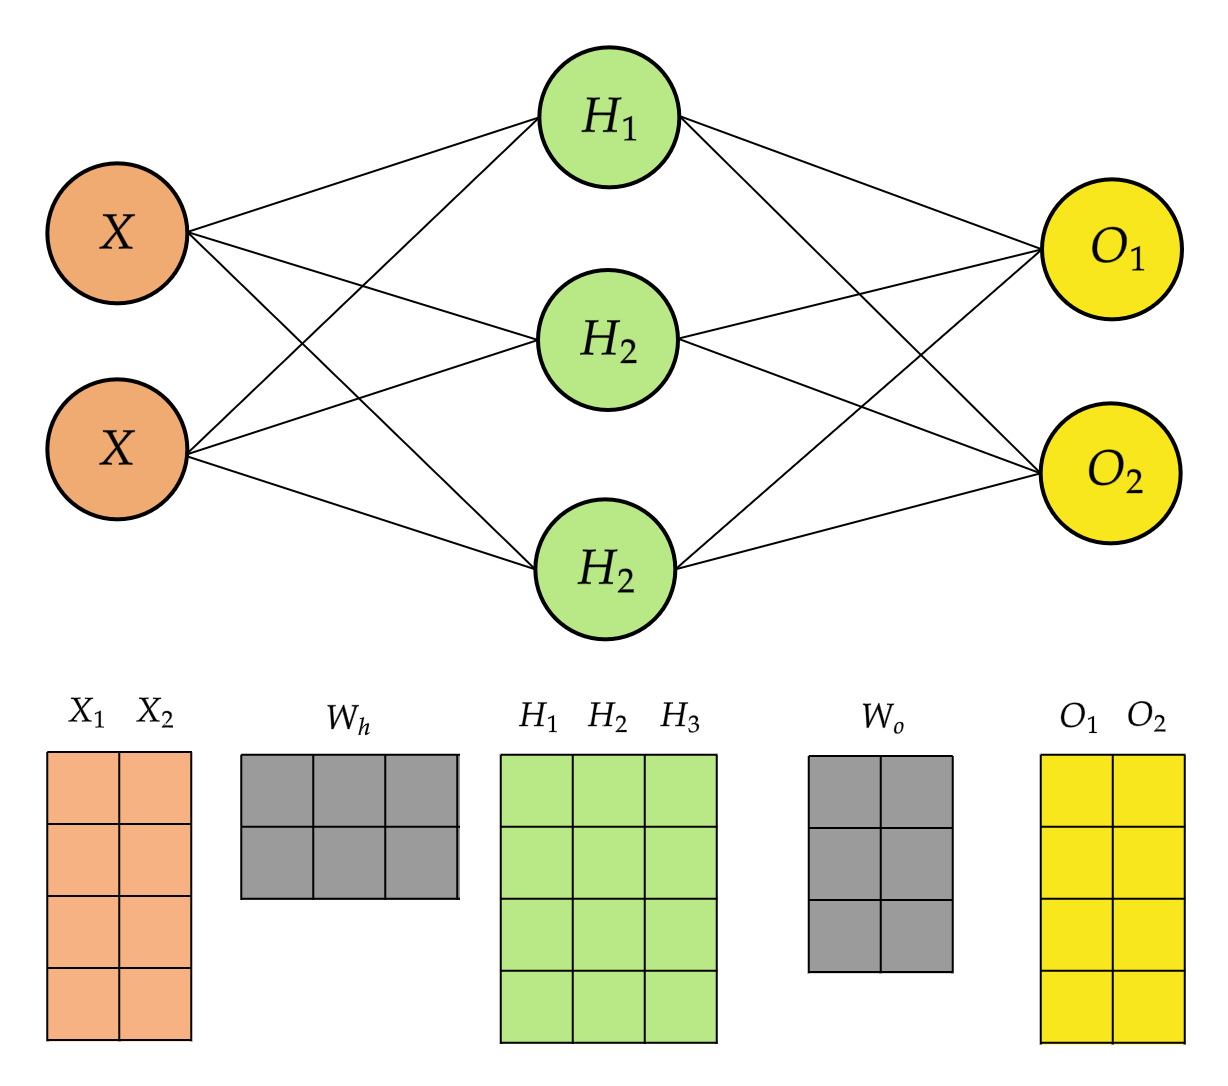
\includegraphics[width=0.8\linewidth]{fig/nn_feedforward_dyn_resizing.png}
    \caption{แผนภาพขนาดของเมทริกซ์ที่สามารถปรับขนาดได้แบบไดนามิกส์}
    \label{fig:nn_ff_dyn_resize}
\end{figure}

\begin{figure}[htbp]
    \centering
    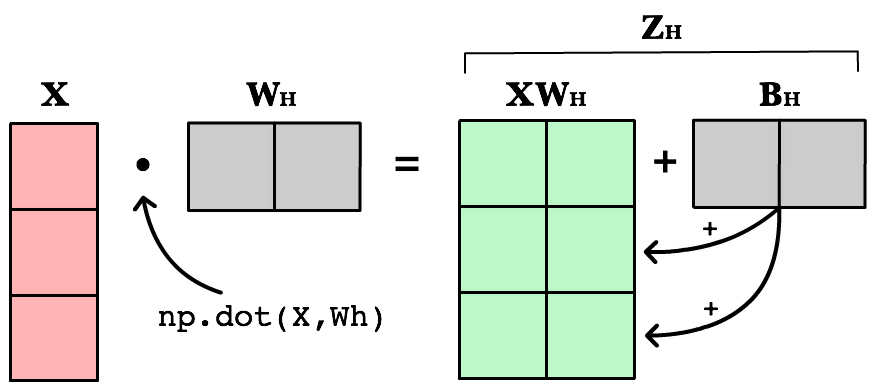
\includegraphics[width=0.8\linewidth]{fig/nn_feedforward_matrix_weighted_input.png}
    \caption{แผนภาพการดำเนินการคูณเมทริกซ์น้ำหนักและการเพิ่มความโน้มเอียง}
    \label{fig:nn_ff_mat_w}
\end{figure}

%--------------------------
\subsection{การแผ่กระจายแบบย้อนกลับ}
\label{ssec:backprop}
\idxboth{การแผ่กระจายการเรียนรู้!การแผ่กระจายแบบย้อนกลับ}{Propagation!Backpropagation}
%--------------------------

การแผ่กระจายแบบย้อนกลับ (Backpropagation) เป็นหัวใจหลักของ Deep Learning เลยก็ว่าได้ นั่นก็เพราะว่าถ้าหากว่า Neural Network 
(ใน Deep Learning เราเน้นที่ Neural Network) ที่เราสร้างขึ้นนั้นมีแต่การเรียนรู้แบบแผ่ไปข้างหน้าโดยที่พารามิเตอร์ของโมเดลไม่มีการถูกปรับ
(Optimization) ให้เหมาะสมนั้น ความสามารถในการทำนายค่าก็จะไม่เพิ่มขึ้น ดังนั้นถ้าหากเราต้องการเพิ่มความสามารถในการเรียนรู้ของโมเดล 
การแผ่กระจายย้อนกลับ (เรียกสั้น ๆ ว่า Backprop) นั้นจึงจำเป็นมาก เพราะการทำ Backprop นั้นเป็นการปรับค่า Weight โดยการเทียบกับ Loss
Function ของเรา ซึ่ง Loss Function นี้เองที่เป็นตัวบอกความแตกต่างระหว่างค่าเอาต์พุตหรือค่าที่เราทำนาย (Prediction) กับค่าอ้างอิง 
(Reference) ดังนั้นถ้าหากเราต้องการที่จะปรับค่า Weight เพื่อให้มี Loss ที่น้อยลงเรื่อย ๆ เราสามารถทำได้โดยการหาอนุพันธ์ของ Loss 
เทียบกับ Weight แต่ว่าใน Neural Network นั้นมี Weight หลายค่ามาก ดังนั้นเราจึงจำเป็นต้องใช้กฎลูกโซ่เข้ามาช่วยในการหาอนุพันธ์หลายตัวแปร
\idxboth{กฎลูกโซ่}{Chain Rule}

\begin{figure}[htbp]
    \centering
    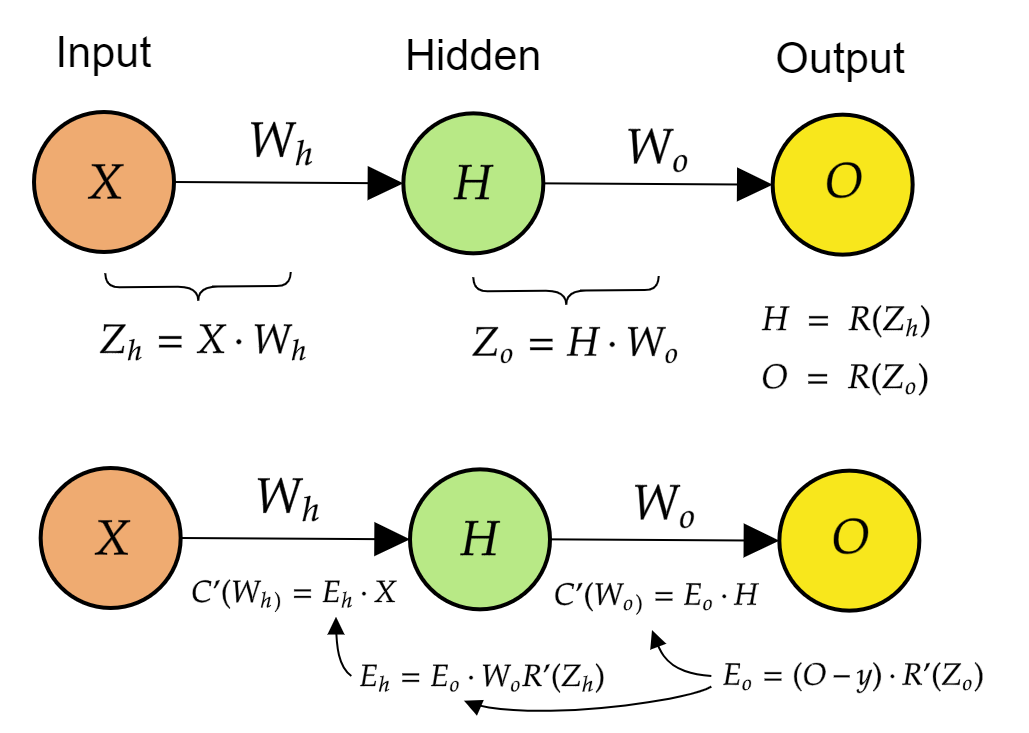
\includegraphics[width=0.8\linewidth]{fig/nn_backprop.png}
    \caption{การคำนวณการแผ่กระจายแบบย้อนกลับจากชั้นเอาต์พุตไปยังชั้นอินพุน}
    \label{fig:nn_bp}
\end{figure}

สำหรับการหาอนุพันธ์ของ Loss เทียบกับ Weight นั้นเราสามารถกระจายอนุพันธ์ออกมาให้อยู่ในรูปที่มี Weight จากแต่ละชั้น (Layer) ได้ 
เมื่อเราทำการหาอนุพันธ์นั้นเราจะต้องทำการหาของ Weight ที่อยู่ในชั้นท้ายสุดไล่ไปหาชั้นแรกสุด (ดูตามภาพที่ \ref{fig:nn_bp})
นั่นจึงเป็นเหตุผลที่เราเรียกการแผ่กระจายแบบนี้ว่าการแผ่กระจายย้อนกลับเพราะว่าเราทำการปรับ Weight ของ Hidden Layer จากหลังไปหน้านั่นเอง

\begin{algorithm}[ht]
    \caption{อัลกอริทึมของ Backpropagation สำหรับ Neural Network ซึ่งแสดงด้วย Computation Graph $G = (V,E)$.}
    \label{alg:backprop}
    \begin{enumerate}
        \item For a sample $(x_n ,y^*_n)$, propagate the input $x_n$ through the
        network to compute the outputs $(v_{i_1}, \ldots, v_{i_{|V|}})$ (in topological order).
        %\begin{enumerate}[(a)]
        %  \item Given a topological sort $V = (v_{i_1},\ldots,v_{i_{|V|}})$,
        %  sequentially compute the layers' outputs, also denoted by $v_{i_j}$.
        %  \item Then $y(x_n;w) = v_{i_{|V|}}$ is the network's output.
        %\end{enumerate}

        \item Compute the loss $\mathcal{L}_n := \mathcal{L}(v_{i_{|V|}}, y_n^*)$
        and its gradient
        \begin{align}
        \frac{\partial \mathcal{L}_n}{\partial v_{i_{|V|}}}.
        \end{align}

        \item For each $j = |V|,\ldots,1$ compute
        \begin{align}
        \frac{\partial \mathcal{L}_n}{\partial w_j} =
        \frac{\partial \mathcal{L}_n}{\partial v_{i_{|V|}}} \prod_{k = j + 1}^{|V|} 
        \frac{\partial v_{i_k}}{\partial v_{i_{k - 1}}}
        \frac{\partial v_{i_j}}{\partial w_j}.
        \end{align}
        where $w_j$ refers to the weights in node $i_j$.
    \end{enumerate}
\end{algorithm}

สำหรับผู้ที่สนใจอัลกอริทึมของ Backprop สามารถดูได้เพิ่มเติมได้ที่ \ref{alg:backprop}

%--------------------------
\section{ฟังก์ชันกระตุ้น}
\label{sec:act_func}
\idxboth{ฟังก์ชันกระตุ้น}{Activation Function}
%--------------------------

ฟังก์ชันกระตุ้น (Activation Function) หรือเรียกอีกชื่อว่า ฟังก์ชันการส่งต่อ (Transfer Function) เป็นหนึ่งใน Hyperparameters 
ที่สำคัญมาก ๆ ของ Neural Network นั่นก็เพราะว่าฟังก์ชันกระตุ้นนี้จะทำหน้าที่ในการปรับให้ฟังก์ชันที่ใช้อธิบายความสัมพันธ์ระหว่างข้อมูล $x$ 
และ $y$ นั้นมีความไม่เป็นเส้นตรง (Nonlinearity) อธิบายง่าย ๆ ก็คือ Neural Network ที่ไม่มีการใช้ฟังก์ชันกระตุ้นก็จะไม่ต่างอะไรจากโมเดล
Linear Regression แบบเส้นตรงนั่นเอง โดยสิ่งที่ฟังก์ชันกระตุ้นทำก็คือจะทำการคำนวณทำนายค่าของเอาต์พุตออกมา ซึ่งรูปแบบของฟังก์ชันกระตุ้น%
ก็จะมีหลากหลายรูปแบบ เนื่องจากปัญหาของข้อมูลในโลกความเป็นจริงมีลักษณะเป็นแบบสมการเส้นตรงน้อยมาก ฟังก์ชันกระตุ้นจึงเป็นเหมือนเจ้าหน้าที่%
ที่คอยตัดสินใจว่าหน่วยเรียนรู้ (Node) ควรจะถูกกระตุ้นเพื่อให้เกิดการเรียนรู้หรือไม่ โดยพิจารณาจากค่าผลรวมของอินพุต, ค่า Weight, และค่า Bias 
โดยฟังก์ชันกระตุ้นถูกนำไปใช้ทั้งกับ Node ใน Hidden Layer และใน Output Layer ซึ่ง Node ในทั้งสองชั้นนี้อาจจะใช้ฟังก์ชันกระตุ้นที่เหมือน%
หรือต่างกันก็ได้ ขึ้นอยู่กับความสามารถและพฤติกรรมของการเรียนรู้ของชั้นนั้น ๆ 
\idxboth{ฟังก์ชันการส่งต่อ}{Transfer Function}

โดยส่วนมากแล้วเรามักจะใช้ฟังก์ชันกระตุ้นแบบไม่เป็นเชิงเส้นกับ Hidden Layer เหตุผลก็คือเนื่องจากว่าใน Hidden Layer จะมีการคำนวณแบบ%
การรวมเชิงเส้น ถ้าฟังก์ชันกระตุ้นของ Hidden Layer มีการคำนวณแบบเชิงเส้นอีก จะเป็นการเรียนรู้การทำงานที่ซ้ำซ้อนกับการคำนวณแบบการรวม%
เชิงเส้นใน Output Layer และจะส่งผลให้ผลลัพธ์นั้นเทียบเท่ากับ Logistic Regression 

การเลือกฟังก์ชันกระตุ้นนั้นสำคัญมาก ถ้าหากเราเลือกฟังก์ชันกระตุ้นที่ไม่เหมาะสมหรือเลือกผิดชีวิตอาจเปลี่ยนได้เลย เช่น หนึ่งในปัญหาที่มักกวนใจ%
ผู้ที่ใช้ Neural Network อยู่เสมอนั่นก็คือ Vanishing Gradient Problem ซึ่งเป็นปัญหาที่เกิดขึ้นในระหว่างการฝึกสอนโมเดลโดยที่ Gradient 
ของ Loss Function นั้นมีขนาดเล็กลงเรื่อย ๆ จนเท่ากับ 0 ทำให้ Weight ไม่ถูกอัพเดทอีกต่อไป ส่งผลให้การฝึกสอนโมเดลไม่สามารถทำต่อได้
โดยวิธีการแก้ปัญหานั้นก็มีอยู่ด้วยกันหลายวิธี เช่น การทำ Weight Initialization หรือการใช้ Batch Normalization และการใช้ฟังก์ชัน 
ReLU แทนฟังก์ชัน Sigmoid ก็สามารถแก้ปัญหาได้เช่นเดียวกัน นอกจาก Vanishing Gradient Problem แล้วยังมีปัญหาที่ตรงข้ามกันนั่นก็คือ 
Exploding Gradient Problem ซึ่งเกิดขึ้นในระหว่างการฝึกสอนโมเดลเช่นเดียวกัน แต่จะเป็นกรณีที่ Gradient ของ Loss Function มีขนาด%
ใหญ่ขึ้นเรื่อย ๆ จนเข้าใกล้ค่าอนันต์ (Infinity) ซึ่งจะถูกกำหนดหรือนิยามเป็น Not a Number (NaN) หมายความว่าตัวเลขมีค่าที่เยอะเกินหน่วย%
ความจำของระบบที่ได้ถูกจัดสรรค์ไว้ (Allocation) ทำให้ไม่สามารถฝึกสอนโมเดลต่อไปได้
\idxen{Vanishing Gradient Problem}
\idxen{Exploding Gradient Problem}
\idxen{Not a Number (NaN)}

ฟังก์ชันกระตุ้นที่ถูกใช้ใน Neural Network มีหลากหลายรูปแบบ ตัวอย่างดังต่อไปนี้

\begin{itemize}
    \item \textbf{Binary Step} ฟังก์ชันไบนารี่เป็นฟังก์ชันกระตุ้นแบบที่ง่ายที่สุด โดยให้ค่าเอาต์พุตเพียงแค่ 2 ค่าเท่านั้นคือ 0 กับ 1
    ถ้าอินพุตมีค่าน้อยกว่าหรือเท่ากับ 0 เอาต์พุตที่ได้จะเป็น 0 และถ้าอินพุตมีค่ามากกว่า 0 เอาต์พุตที่ได้ก็จะเป็น 1
    \idxen{Activation Function!Binary Step}
    \begin{equation}
        R(z) = \left\{
            \begin{array}{lll}
                0 & for & z \leq 0  \\
                1 & for & z > 0
            \end{array}
        \right.
    \end{equation}

    \item \textbf{Linear} ฟังก์ชันเส้นตรงโดยที่ Activation นั้นเป็นสัดส่วนโดยตรงกับอินพุต (นำค่า Weights มารวมกันตรง ๆ)
    \idxen{Activation Function!Linear}
    \begin{figure}[htbp]
        \centering
        \begin{subfigure}{0.5\textwidth}
            \centering
            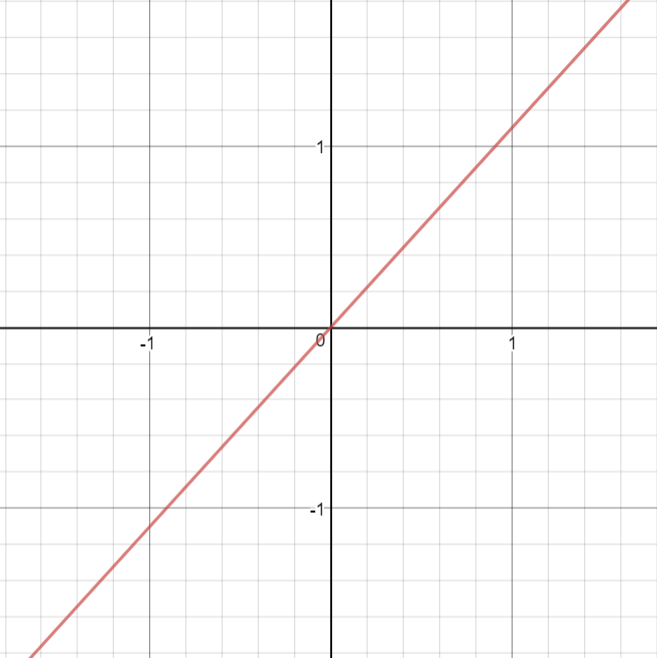
\includegraphics[width=0.9\linewidth]{fig/actfunc_linear.png}
            \caption{%
                \begin{equation}
                    \begin{split}R(z,m) = \begin{Bmatrix} z*m \\
                    \end{Bmatrix}\end{split}
                \end{equation}
            }
            \label{fig:actfunc_lin}
        \end{subfigure}%
        \begin{subfigure}{0.5\textwidth}
            \centering
            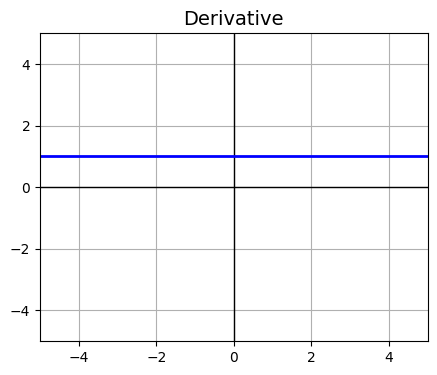
\includegraphics[width=0.9\linewidth]{fig/actfunc_linear_der.png}
            \caption{%
                \begin{equation}
                    \begin{split}R'(z,m) = \begin{Bmatrix} m \\
                    \end{Bmatrix}\end{split}
                \end{equation}
            }
            \label{fig:actfunc_lin_der}
        \end{subfigure}
    \end{figure}
    ข้อดี:
    \begin{itemize}
        \item เป็น Activation แบบที่เป็นช่วง (Range) ซึ่งมีประสิทธิดีกว่าฟังก์ชันแบบไบนารี่
    \end{itemize}
    ข้อเสีย:
    \begin{itemize}
        \item อนุพันธ์ของฟังก์ชันนี้เป็นค่าคงที่ นั่นคือเกรเดียนต์ของฟังก์ชันนี้จึงไม่มีความสัมพันธ์กับอินพุต
    \end{itemize}

    \item \textbf{ELU} ย่อมาจาก Exponential Linear Unit เป็นฟังก์ชันที่พยายามทำให้ Cost นั้นลู่เข้าสู่ศูนย์และให้ประสิทธิภาพที่ดี%
    มากขึ้น โดยพารามิเตอร์ที่ควบคุมประสิทธิภาพของ ELU ก็คือ $\alpha$ ซึ่งควรจะต้องมีค่าเป็นบวกเสมอ
    \idxen{Activation Function!ELU}
    \begin{figure}[htbp]
        \centering
        \begin{subfigure}{0.5\textwidth}
            \centering
            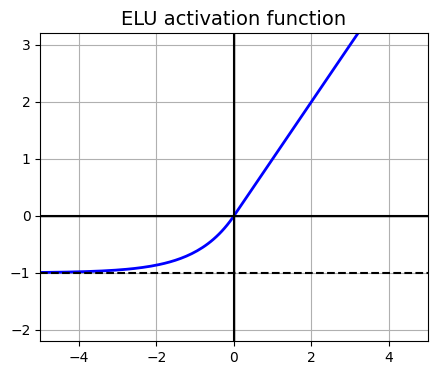
\includegraphics[width=0.9\linewidth]{fig/actfunc_elu.png}
            \caption{%
                \begin{equation}
                    \begin{split}R(z) = \begin{Bmatrix} z & z > 0 \\
                        \alpha (e^z – 1) & z <= 0 \end{Bmatrix}\end{split}
                \end{equation}
            }
            \label{fig:actfunc_elu}
        \end{subfigure}%
        \begin{subfigure}{0.5\textwidth}
            \centering
            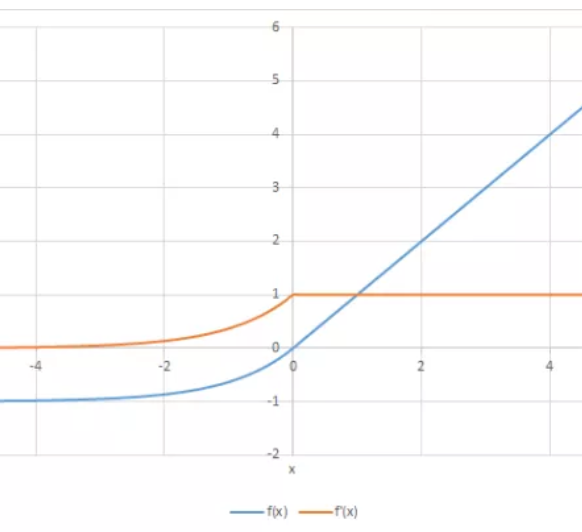
\includegraphics[width=0.9\linewidth]{fig/actfunc_elu_der.png}
            \caption{%
                \begin{equation}
                    \begin{split}R'(z) = \begin{Bmatrix} 1 & z>0 \\
                        \alpha e^z & z<0 \end{Bmatrix}\end{split}
                \end{equation}
            }
            \label{fig:actfunc_elu_der}
        \end{subfigure}
    \end{figure}
    ข้อดี:
    \begin{itemize}
        \item ฟังก์ชัน ELU นั้นมีความราบเรียบ (Smooth) ยอ่างช้า ๆ จนกว่าค่าเอาต์พุตของฟังก์ชันจะมีค่าเท่ากับ $-\alpha$
        
        \item เราสามารถใช้ฟังก์ชัน ELU แทน ReLU ได้ในบางกรณีเพราะทั้งสองฟังก์ชันนี้มีความคล้ายกันมาก
        
        \item ELU สามารถให้เอาต์พุตที่มีค่าเป็นลบได้ แต่ว่าฟังก์ชัน ReLU นั้นให้เอาต์พุตที่เป็นบวกเสมอ
    \end{itemize}
    ข้อเสีย:
    \begin{itemize}
        \item สำหรับกรณีที่ $x > 0$ การใช้ฟังก์ชัน ELU อาจจะทำให้เกิดปัญหาได้ (เกิดการระเบิดหรือ Blow Up) จะทำให้เอาต์พุตอยู่ในช่วง 
        $[0,\infty)$
    \end{itemize}

    \item \textbf{ReLU}\autocite{glorot2011} ย่อมาจาก Rectified Linear Units เป็นฟังก์ชันกระตุ้นที่มีความสามารถในการ%
    เรียนรู้ฟังก์ชันหรือความสัมพันธ์ที่ไม่เป็นเชิงเส้นได้ดีมาก (ดีกว่าฟังก์ชัน Sigmoid)
    \idxen{Activation Function!ReLU}
    \begin{figure}[htbp]
        \centering
        \begin{subfigure}{0.5\textwidth}
            \centering
            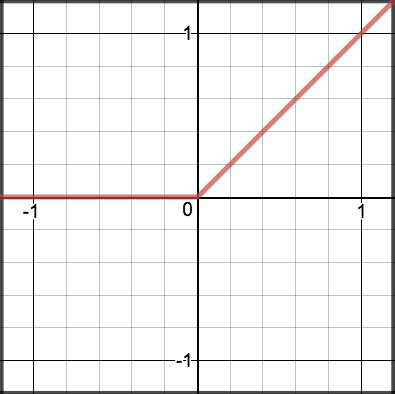
\includegraphics[width=0.9\linewidth]{fig/actfunc_relu.png}
            \caption{%
                \begin{equation}
                    \begin{split}R(z) = \begin{Bmatrix} z & z > 0 \\
                        0 & z <= 0 \end{Bmatrix}\end{split}
                \end{equation}
            }
            \label{fig:actfunc_relu}
        \end{subfigure}%
        \begin{subfigure}{0.5\textwidth}
            \centering
            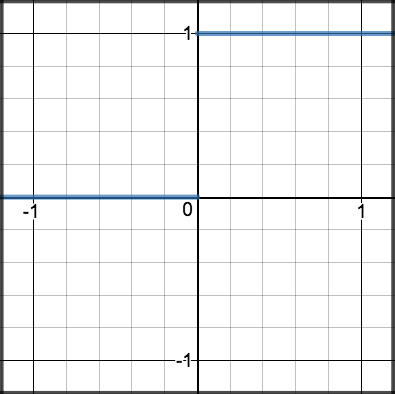
\includegraphics[width=0.9\linewidth]{fig/actfunc_relu_der.png}
            \caption{%
                \begin{equation}
                    \begin{split}R'(z) = \begin{Bmatrix} 1 & z>0 \\
                        0 & z<0 \end{Bmatrix}\end{split}
                \end{equation}
            }
            \label{fig:actfunc_relu_der}
        \end{subfigure}
    \end{figure}

    ข้อดี:
    \begin{itemize}
        \item ReLU แก้ปัญหา Vanishing Gradient Problem ได้
        
        \item ฟังก์ชัน ReLU นั้นเรียบง่ายกว่า Sigmoid และ Tanh จึงทำให้การคำนวณของฟังก์ชัน ReLU นั้นเร็วกว่าและสิ้นเปลืองน้อยกว่า 
    \end{itemize}
    ข้อเสีย:
    \begin{itemize}
        \item ควรใช้ฟังก์ชัน ReLU เฉพาะในชั้นซ่อน (Hidden Layer) ของ Neural Network เท่านั้น
        
        \item ในระหว่างการฝึกสอนโมเดลด้วย ReLU ของบางกรณีนั้น การคำนวณ Gradient อาจจะมีปัญหาได้
        
        \item สำหรับการ Activation ของฟังก์ชัน ReLU ในช่วงที่ิอินพุต $x < 0$ ค่า Gradient จะเท่ากับ 0 เพราะว่า Weights 
        นั้นจะไม่ถูกปรับค่าในระหว่างการทำ Gradient Descent

        \item เนื่องจากว่า ReLU นั้นมีความคล้ายกับ ELU ดังนั้นการใช้ฟังก์ชัน ReLU อาจจะทำให้เกิดปัญหาได้เพราะว่ามี Range คือ 
        $[0,\infty)$
    \end{itemize}

    \item \textbf{LeakyReLU}\autocite{he2015} เป็นฟังก์ชันที่ถุกพัฒนาต่อมาจาก ReLU ซึ่งได้มีการปรับปรุงให้มีประสิทธิภาพมากขึ้น%
    โดยทำการปรับค่าเอาต์พุต ในกรณีที่อินพุต $z < 0$ ค่าเอาต์พุตจะไม่เป็น 0 อีกต่อไป แต่จะเป็น $\alpha z$ แทน ซึ่งทำให้มีความ General 
    มากกว่าฟังก์ชัน ReLU (โดยปกติแล้วจะกำหนดให้ $\alpha = 0.01$)
    \idxen{Activation Function!LeakyReLU}
    \begin{figure}[htbp]
        \centering
        \begin{subfigure}{0.5\textwidth}
            \centering
            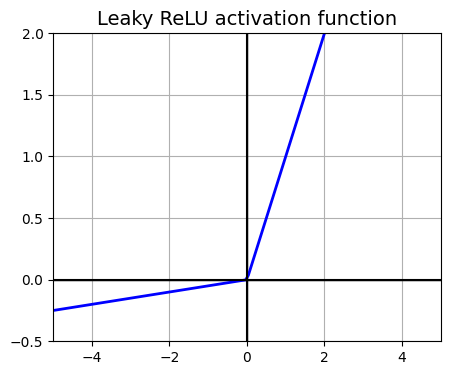
\includegraphics[width=0.9\linewidth]{fig/actfunc_leakyrelu.png}
            \caption{%
                \begin{equation}
                    \begin{split}R(z) = \begin{Bmatrix} z & z > 0 \\
                        \alpha z & z <= 0 \end{Bmatrix}\end{split}
                \end{equation}
            }
            \label{fig:actfunc_leakyrelu}
        \end{subfigure}%
        \begin{subfigure}{0.5\textwidth}
            \centering
            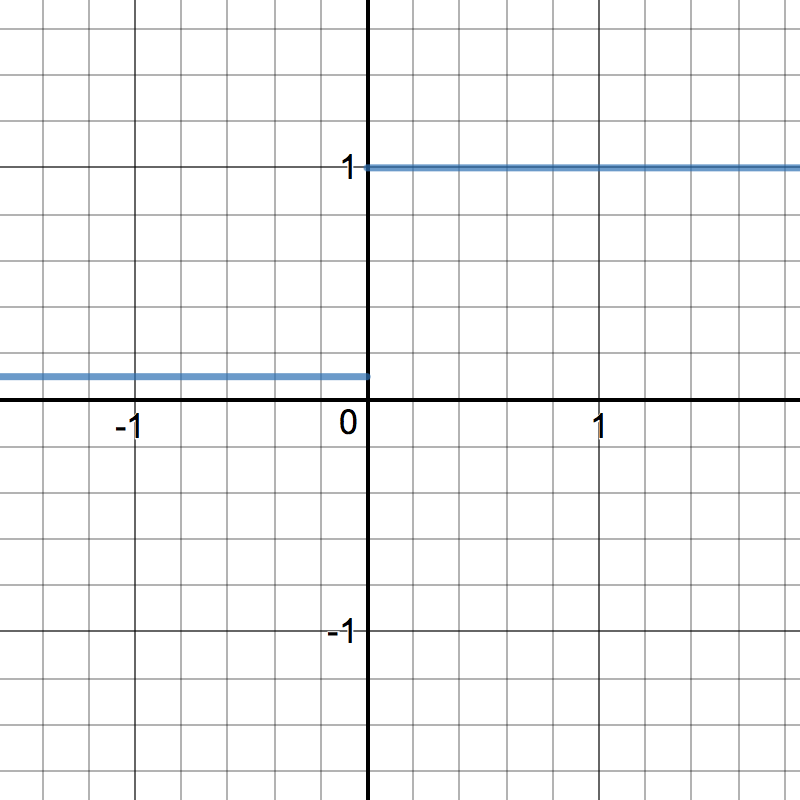
\includegraphics[width=0.9\linewidth]{fig/actfunc_leakyrelu_der.png}
            \caption{%
                \begin{equation}
                    \begin{split}R'(z) = \begin{Bmatrix} 1 & z>0 \\
                        \alpha & z<0 \end{Bmatrix}\end{split}
                \end{equation}
            }
            \label{fig:actfunc_leakyrelu_der}
        \end{subfigure}
    \end{figure}

    ข้อดี:
    \begin{itemize}
        \item LeakyReLU สามารถแก้ปัญหาของ ReLU ได้โดยการทำให้มีเอาต์พุตเป็น Slope ที่มีความชันน้อย ๆ
    \end{itemize}
    ข้อเสีย:
    \begin{itemize}
        \item เนื่องจากว่า Range ของ LeakyReLU นั้นเป็นเส้นตรง ดังนั้นจึงไม่เหมาะที่จะนำฟังก์ชันนี้มาใช้กับปัญหา Classification 
        ที่ซับซ้อน ซึ่งในกรณีดังกล่าวการใช้ฟังก์ชัน Sigmoid หรือ Tanh จะเหมาะสมกว่า
    \end{itemize}

    \item \textbf{Sigmoid}\autocite{wilson1972} เป็นหนึ่งในฟังก์ชันกระตุ้นที่มีประสิทธิภาพสูงมากในการนำมาใช้กับ Neural Network 
    โดยฟังก์ชันนี้ทำการนำค่าอินพุตมาคำนวณโดยใช้ฟังก์ชัน Exponential ซึ่งให้ค่าเอาต์พุตที่อยู่ระหว่าง $(0, 1)$ ดังนั้นจึงทำให้ฟังก์ชันนี้มี%
    คุณสมบัติหลายอย่างที่ฟังก์ชันกระตุ้นควรมี เช่น ความไม่เป็นเส้นตรง, มีความต่อเนื่อง, สามารถหาอนุพันธ์ได้ตลอดช่วง, มีความโมโนโทนิค 
    (Monotonic) และมีเอาต์พุตที่อยู่ในช่วงที่แน่นอน
    \idxen{Activation Function!Sigmoid}
    \begin{figure}[htbp]
        \centering
        \begin{subfigure}{0.5\textwidth}
            \centering
            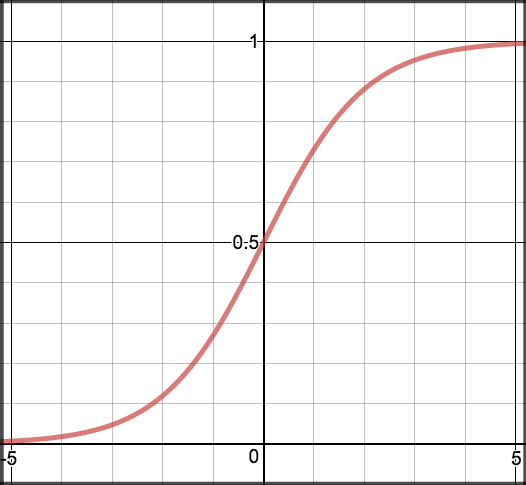
\includegraphics[width=0.9\linewidth]{fig/actfunc_sigmoid.png}
            \caption{%
                \begin{equation}
                    S(z) = \frac{1} {1 + e^{-z}}
                \end{equation}
            }
            \label{fig:actfunc_sigmoid}
        \end{subfigure}%
        \begin{subfigure}{0.5\textwidth}
            \centering
            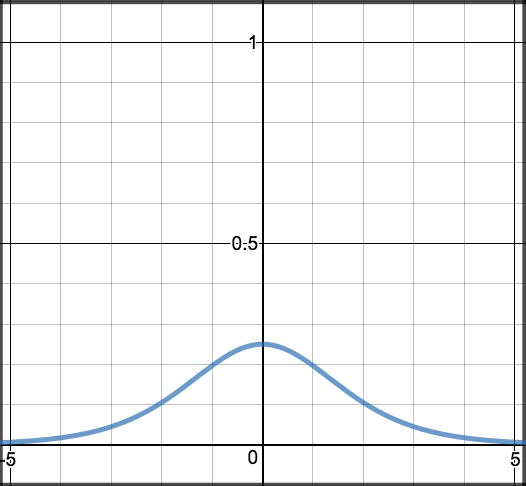
\includegraphics[width=0.9\linewidth]{fig/actfunc_sigmoid_der.png}
            \caption{%
                \begin{equation}
                    S'(z) = S(z) \cdot (1 - S(z))
                \end{equation}
            }
            \label{fig:actfunc_sigmoid_der}
        \end{subfigure}
    \end{figure}

    ข้อดี:
    \begin{itemize}
        \item มีความไม่เป็นเส้นตรง
        
        \item ฟังก์ชัน Sigmoid มีอนุพันธืที่มีความราบเรียบ
        
        \item เหมาะสำหรับการนำไปใช้กับโจทย์ Classification
        
        \item ฟังก์ชัน Sigmoid มี Range คือ $(0,1)$ ซึ่งไม่เหมือนกับ Range ของฟังก์ขันเส้นตรงซึ่งมีค่าที่ไม่อยู่ในช่วงที่แน่นอนนั่นคือ 
        $-\infty, \infty$
    \end{itemize}
    ข้อเสีย:
    \begin{itemize}
        \item กรณีที่ค่าอินพุตมีค่ามาก ๆ ค่าเอาต์พุตของ Sigmoid จะมีการเปลี่ยนแปลงที่น้อยมาก ๆ
        
        \item ฟังก์ชัน Sigmoid ทำให้เกิดปัญหา Vanishing Gradient Problem ได้
        
        \item เอาต์พุตของฟังก์ชัน Sigmoid มีจุดกึ่งกลางที่ไม่ใช่ 0 (Not Zero-centered) ทำให้การเปลี่ยนแปลงของ Gradient 
        นั้นมีค่าที่อยู่ห่างจากฟังก์ชันเดิมมาก ๆ ซึ่งเป็นสาเหตุที่ทำให้การ Optimization นั้นยากขึ้น

        \item ในบางกรณีนั้นการใช้ฟังก์ชัน Sigmoid จะทำให้การเรียนรู้ของ Neural Network นั้นทำได้ยากและช้า
    \end{itemize}

    \item \textbf{Tanh} เป็นฟังก์ชันกระตุ้นแบบไม่เป็นเชิงเส้นที่มี Range อยู่ระหว่าง -1 ถึง 1 $(-1, 1)$ สิ่งที่ฟังก์ชัน Tanh ต่างจาก%
    ฟังก์ชัน Sigmoid ก็คือเอาต์พุตมีจุดกึ่งกลางอยู่ที่ 0 (Zero-centered) จึงทำให้ฟังก์ชันนี้ถูกใช้มากกว่า Sigmoid นั่นเอง
    \idxen{Activation Function!Tanh}
    \begin{figure}[htbp]
        \centering
        \begin{subfigure}{0.5\textwidth}
            \centering
            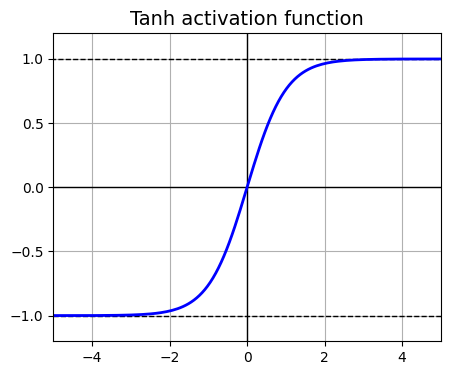
\includegraphics[width=0.9\linewidth]{fig/actfunc_tanh.png}
            \caption{%
                \begin{equation}
                    tanh(z) = \frac{e^{z} - e^{-z}}{e^{z} + e^{-z}}
                \end{equation}
            }
            \label{fig:actfunc_tanh}
        \end{subfigure}%
        \begin{subfigure}{0.5\textwidth}
            \centering
            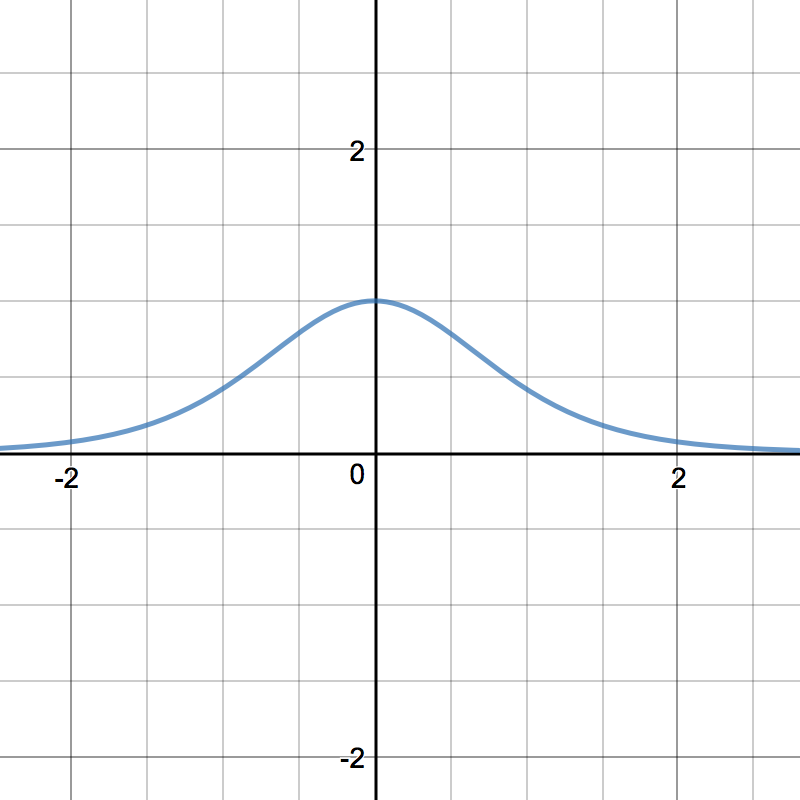
\includegraphics[width=0.9\linewidth]{fig/actfunc_tanh_der.png}
            \caption{%
                \begin{equation}
                    tanh'(z) = 1 - tanh(z)^{2}
                \end{equation}
            }
            \label{fig:actfunc_tanh_der}
        \end{subfigure}
    \end{figure}

    ข้อดี:
    \begin{itemize}
        \item Gradient ของฟังก์ชัน Tanh มีค่าการเปลี่ยนแปลงของ Slope ที่ดีกว่า Gradient ของฟังก์ชัน Sigmoid
    \end{itemize}
    ข้อเสีย:
    \begin{itemize}
        \item ฟังก์ชัน Tanh ยังคงมีปัญหาเกี่ยวกับ Vanishing Gradient Problem
    \end{itemize}

    \item \textbf{Softmax} เป็นฟังก์ชันกระตุ้นที่คำนวณ Probability Distribution ของเหตุการณ์ทั้งหมด $n$ เหตุการณ์ที่แตกต่างกัน 
    กล่าวง่าย ๆ คือฟังก์ชันนี้ทำการคำนวณคลาส (Class) ของเป้าหมายของเราให้อยู่ในรูปของค่าความน่าจะเป็นซึ่งจะถูกนำมาใช้ในการกำหนด%
    หรือทำนายคลาสของเหตุการณ์ที่เราสนใจ
    \idxen{Activation Function!Softmax}
    \begin{equation}
        \sigma(z_i) = \frac{e^{z_{i}}}{\sum_{j=1}^K e^{z_{j}}} \ \ \ for\ i=1,2,\dots,K
    \end{equation}
\end{itemize}

ถ้าหากผู้อ่านต้องการศึกษาการเขียนโค้ดสำหรับพลอตกราฟฟังก์ชันกระตุ้นแบบต่าง ๆ สามารถดูได้ที่ 
\url{https://github.com/siebenrock/activation-functions}

%--------------------------
\section{ฟังก์ชันสูญเสีย}
\label{sec:loss_func}
\idxboth{ฟังก์ชันสูญเสีย}{Loss Function}
\idxboth{ฟังก์ชันต้นทุน}{Cost Function}
\idxboth{ฟังก์ชันความคลาดเคลื่อน}{Error Function}
%--------------------------

%--------------------------
\subsection{ความสำคัญของฟังก์ชันสูญเสีย}
%--------------------------

ฟังก์ชันสูญเสีย (Loss Function หรือ Cost Function) เป็นฟังก์ชันความคลาดเคลื่อน (Error Function) รูปแบบหนึ่งซึ่งมีความสำคัญมากใน 
Neural Network (จริง ๆ แล้วเราจะถือว่า Loss Function กับ Error Function นั้นเป็นสิ่งเดียวกันก็ได้) เพราะว่าเป็นฟังก์ชันคณิตศาสตร์ที่ 
Map ค่าเหตุการณ์ (Event) จากอินพุตหลาย ๆ ตัว ให้ออกมาเป็นค่า Error เพียงแค่เดียวซึ่งเป็นค่าที่ระบุถึง Cost ของเหตุการณ์นั้น ๆ โดย Loss 
Function ถูกใช้ในการทำ Optimization นั่นก็คือการหาวิธีที่ทำให้ค่าเอาต์พุตของของ Loss Function นั้นมีค่าน้อยที่สุด เรียกว่า Minimization 

\begin{figure}[htbp]
    \centering
    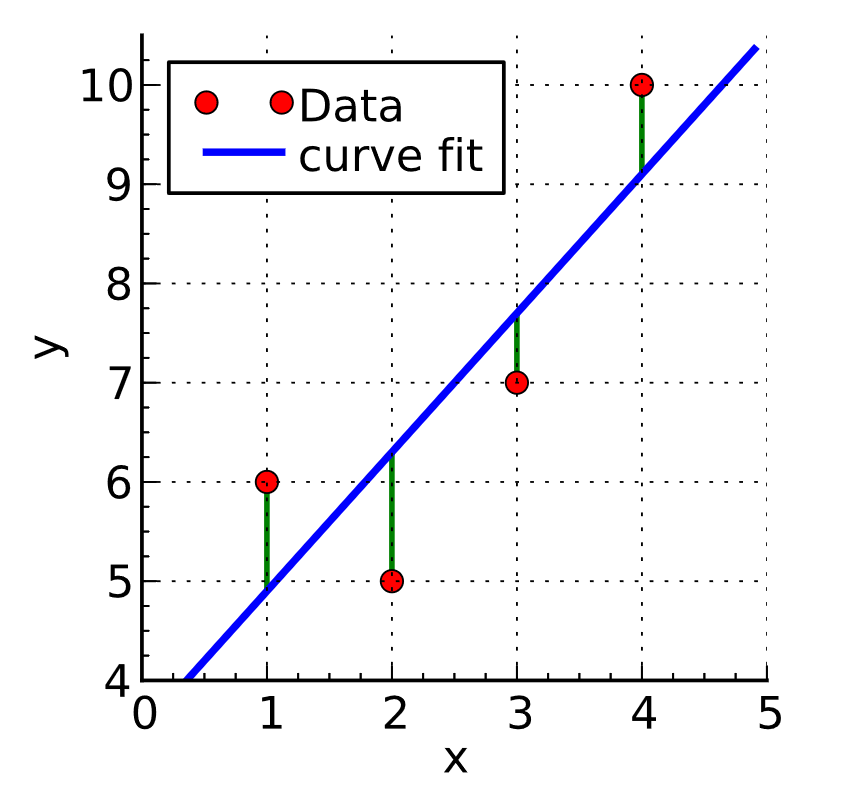
\includegraphics[width=0.7\linewidth]{fig/least-squares-fitting.png}
    \caption{แสดงการทำ Least Squares Fitting โดยมีพิกัดตำแหน่งของข้อมูลแต่ละตัว (จุดสีแดง) ดังนี้ $(1,6)$, $(2,5)$, $(3,7)$ 
    และ $(4,10)$ และเส้นตรงที่ได้จากการประมาณค่าด้วยวิธี Least Squares Estimation นั้น (เส้นสีน้ำเงิน) (เครดิตภาพ: 
    \url{https://en.wikipedia.org/wiki/Linear_least_squares})}
    \label{fig:least_square_fitting}
\end{figure}

แนวคิดของ Loss Function ก็คือเราต้องการตัวชี้วัดที่เป็นตัวเลขค่าเดียวที่สามารถบอกได้ว่าโมเดล ML ที่ฝึกสอนมาแล้วนั้นทำงานได้ดีแค่ไหน 
โดยถ้าหากดูจากภาพที่ \ref{least_square_fitting} โดยเปรียบเทียบเอาต์พุตของโมเดลนั่นก็คือ $\hat{y}$ กับข้อมูลเอาต์พุตตัวอย่าง $y$ 
นั่นก็คือจุดสีแดงและมีค่าเส้นน้ำเงินที่เป็นเส้นที่เกิดจากการ Fitting และมีเส้นสีเขียวที่บ่งบอกว่าจุดสีแดงแต่ละจุดนั้นมีการเบี่ยงเบน (Deviation) 
ออกจากเส้นสีน้ำเงินมากน้อยเพียงใด

ตัวอย่างของ Loss Function ที่นิยมใช้ในโจทย์ประเภท Regression ของชุดข้อมูลที่มี $n$ จำนวนข้อมูลและมีค่าเอาต์พุตที่ได้จากการทำนายที่เป็น 
$\hat{y}$ และคำตอบอ้างอิง (Reference หรือ Label) คือ $y$ มีดังต่อไปนี้

\begin{equation}\label{eq:mae}
    \text{MAE} = \frac{1}{n} \sum_{i=1}^{n} | y_{i} - \hat{y}_{i} |
\end{equation}
\idxen{Error Function!MAE}

\begin{equation}\label{eq:mape}
    \text{MAPE} = \frac{1}{n} \sum_{i=1}^{n} \left| \frac{y_{i} - \hat{y}_{i}}{x_{i}} \right| \times 100
\end{equation}
\idxen{Error Function!MAPE}

\begin{equation}\label{eq:mse}
    \text{MSE} = \frac{1}{n} \sum_{i=1}^{n} \left( y_{i} - \hat{y}_{i} \right)^2
\end{equation}
\idxen{Error Function!MSE}

\begin{equation}\label{eq:maxae}
    \text{MaxAE} = \max\{y_{i} - \hat{y}_{i}\}, i = 1, 2, ..., n
\end{equation}
\idxen{Error Function!MaxAE}

\begin{equation}\label{eq:maxape}
    \text{MaxAPE} = \max\left\{\left| \frac{y_{i} - \hat{y}_{i}}{x_{i}} \right| \times 100 \right\}, i = 1, 2, 
    ..., n
\end{equation}
\idxen{Error Function!MaxAPE}

\begin{equation}\label{eq:rmsd}
    \text{RMSD} = \sqrt{ \frac{1}{n} \sum_{i=1}^{n} (y_{i} - \hat{y}_{i})^{2} }
\end{equation}
\idxen{Error Function!RMSD}

\begin{equation}\label{eq:grmsd}
    \text{GRMSD} = \sqrt[2n]{ \prod_{i=1}^{n} (y_{i} - \hat{y}_{i})^{2} }
\end{equation}
\idxen{Error Function!GRMSD}

\begin{equation}\label{eq:gwrmsd}
    \text{GWRMSD} = \sqrt{\frac{\sum_{i=1}^{n} \zeta_{i} (y_{i} - \hat{y}_{i})^{2}}{\sum_{i=1}^{n} \zeta_{i}}}
\end{equation}
\idxen{Error Function!GWRMSD}

\noindent โดยที่ $\zeta_{i} = e^{-(y_{i} - \hat{y}_{i}) / c}$

\begin{equation}\label{eq:huber}
    L_{\delta}=
    \left\{\begin{matrix}
        \frac{1}{2}(y - \hat{y})^{2} & \text{if} \left | (y - \hat{y})  \right | < \delta\\
        \delta ((y - \hat{y}) - \frac1 2 \delta) & \text{otherwise}
    \end{matrix}\right.
\end{equation}
\idxen{Error Function!Huber}

สำหรับ Loss Function ที่ \ref{eq:mae} - \ref{eq:gwrmsd} จะมีความคล้ายคลึงกัน แต่จะต่างกันตรงที่การปรับรูปแบบให้ฟังก์ชันที่เป็นความ%
แตกต่างระหว่างค่าอ้างอิงและค่าทำนายนั้นมีความไว (Sensitivity) ต่อ Outlier ที่ต่างกันไป สำหรับสมการที่ \ref{eq:huber} นั้นคือ Huber
Loss ซึ่งจะมีความไวต่อค่าที่ห่างค่าผิดปกติ (Outlier)\footnote{ค่าผิดปกติหรือ Outlier คือค่าที่อยู่ห่างจากค่าส่วนใหญ่ในชุดข้อมูลมากเกินไป} 
ที่น้อยกว่ากรณีของ MSE (สมการที่ \ref{eq:mse}) เพราะว่าใน MSE เทอม $y_{i} - \hat{y}_{i}$ ถูกกำลังสองอยู่นั่นเอง

ฟังก์ชันสูญเสียสำหรับโจทย์ประเภท Classification

\noindent $\bullet$ Cross-entropy คือการวัดความแตกต่างระหว่างการกระจายตัวของความน่าจะเป็น 2 กลุ่มของตัวแปรแบบสุ่มของเหตุการณ์%
ที่เราสนใจ (กลุ่มหรือ Class ในชุดข้อมูล) โดยกรณีที่มีแค่ 2 Class $(M = 2)$ เรามีชื่อเรียกฟังก์ชันประเภทนี้ว่า Binary Cross-entropy 
และกรณีที่มีมากกว่า 2 Class ($M > 2$) เราจะเรียกว่า Multiclass Cross-entropy ซึ่งทั้งสองแบบมีสมการดังต่อไปนี้

\begin{equation}
    H(p) = -{(y\log(p) + (1 - y)\log(1 - p))}
\end{equation}

\begin{equation}
    H(p) = -\sum_{c=1}^My_{o,c}\log(p_{o,c})
\end{equation}


\noindent โดยที่ $p$ คือความน่าจะเป็นของการสังเกต $o$ ใน Class $c$ และ $y$ คือตัวระบุ Class (เช่น 0 กับ 1)

\noindent $\bullet$ Negative Log-likelihood (NLL)

\begin{equation}
    l(y) = -{\log(p(y))}
\end{equation}

\noindent $\bullet$ Hinge loss

\begin{equation}
    l(y) = max(0, 1 - y \cdot \hat{y})
\end{equation}

\noindent $\bullet$ Kullback-Leibler (KL) Divergence

\begin{equation}
    KL(\hat{y} || y) = \sum_{c=1}^{M}\hat{y}_c \log \bigg( {\frac{\hat{y}_c}{y_c}} \bigg)
\end{equation}

\noindent $\bullet$ Jensen-Shannon (JS) Divergence

\begin{equation}
    JS(\hat{y} || y) = \frac{1}{2}(KL(y||\frac{y+\hat{y}}{2}) + KL(\hat{y}||\frac{y+\hat{y}}{2}))
\end{equation}

%--------------------------
\subsection{คณิตศาสตร์ของฟังก์ชันสูญเสีย}
%--------------------------

ลำดับต่อมาเรามาดูกันที่คณิตศาสตร์ที่อยู่เบื้องหลังของ Loss Function กันครับ โดยจะมาดูว่าเราสามารถทำการปรับค่าพารามิเตอร์ต่าง ๆ ใน Neural 
Network เช่น Weight ได้อย่างไร โดยผู้เขียนจะใช้ตัวอย่างโจทย์ Regression 2 แบบนั่นคือ Linear Regression และ Logistic Regression

%--------------------------
\subsubsection{Linear Regression}
\idxen{Loss Function!Linear Regression}
%--------------------------

เราเริ่มต้นด้วยการกำหนดฟังก์ชันหลักสำหรับการทำ Linear Regression ดังนี้

\fbox{%
\begin{minipage}{0.9\linewidth}
    \begin{align*}
        &\text{Linear Equation}: &&z = Xw + b \\[1.5ex]
        &\text{Activation Function}: &&\text{None} \\[1.5ex]
        &\text{Prediction}: &&\hat{y} = z \\[0.5ex]
        &\text{Loss Function}: &&\mathcal{L} = \frac{1}{2}(\hat{y} - y)^2 \\[0.3ex]
    \end{align*}
\end{minipage}}

เราสามารถเขียนโค้ดของฟังก์ชันด้วยภาษา Python ได้ดังนี้

\begin{lstlisting}[style=MyPython]
import numpy as np

weights = np.random.normal(size = n_features).reshape(n_features, 1)
bias = 0

def linear_regression_inference(inputs):
    return np.matmul(inputs, weights) + bias   

def calculate_error(x, y):
    # Mean Squared Error (Ignore taking an average)
    y_hat = linear_regression_inference(x)
    return 0.5 * (yhat - y)**2 
\end{lstlisting}

นอกจากนี้เรายังสามารถคำนวณอนุพันธ์ (Derivative) ของ Loss Function เทียบกับ $z$ โดยใช้กฎลูกโซ่ได้ดังนี้

\begin{equation}\label{eq:loss_chain_rule}
    \frac{\partial \mathcal{L}}{\partial z} = 
    \frac{\partial \mathcal{L}}{\partial \hat{y}} \frac{\partial \hat{y}}{\partial z}
\end{equation}

\noindent เริ่มต้นด้วยการหาอนุพันธ์ย่อยของ Loss Function เทียบกับค่า Prediction

\begin{equation}\label{eq:der_loss_pred}
    \frac{\partial \mathcal{L}}{\partial \hat{y}} = \hat{y} - y
\end{equation}

\noindent ขั้นตอนต่อมาคือเราหาอนุพันธ์ย่อยของ Prediction เทียบกับ Linear Equation ซึ่งเนื่องจากว่า Linear Equation จริง ๆ 
ก็คือ Prediction นั่่นเอง เราจะได้ว่าอนุพันธ์ย่อยมีค่าเท่ากับ 1

\begin{equation}\label{eq:der_pred_lin_eq}
    \frac{\partial \hat{y}}{\partial z} = 1
\end{equation}

\noindent เมื่อเราทำการคูณสมการที่ \ref{eq:der_loss_pred} กับ \ref{eq:der_loss_pred} เข้าด้วยกัน เราจะได้อนุพันธ์ของ Loss 
Function ตามที่ต้องการ 

\begin{equation}\label{eq:der_loss_lin_eq}
    \frac{\partial \mathcal{L}}{\partial z} = \hat{y} - y
\end{equation}

\noindent จากตัวอย่างข้างต้นนี้ผู้อ่านจะพบว่า Linear Regression นั้นง่ายมาก แต่ตัวอย่างต่อไปจะมีความซับซ้อนมากขึ้นครับ

%--------------------------
\subsubsection{Logistic Regression}
\idxen{Loss Function!Logistic Regression}
%--------------------------

ตัวอย่างที่สองคือกรณีของ Logistic Regression โดยเรากำหนดฟังก์ชันต่าง ๆ ดังนี้

\fbox{%
\begin{minipage}{0.9\linewidth}
    \begin{align*}  
        &\text{Linear Equation}: &&z = Xw + b \\[0.5ex]
        &\text{Activation Function}: &&\sigma(z) = \frac{1}{1 + e^{-z}} \\[0.5ex]
        &\text{Prediction}: &&\hat{y} = \sigma(z) \\[1.5ex]
        &\text{Loss Function}: &&\mathcal{L} = -(y\log\hat{y} + (1-y)\log(1-\hat{y})) \\[0.5ex]
    \end{align*}
\end{minipage}}

\noindent และเขียนโค้ดของฟังก์ชันได้ดังนี้\footnote{โดยทั่วไปแล้วในการคำนวณหา Error ของ Logistic Regression ควรจะทำการใส่%
ค่าคงที่เข้าไปในฟังก์ชัน Log เพื่อป้องกันไม่ให้อินพุตของ Log นั้นเป็น 0}

\begin{lstlisting}[style=MyPython]
import numpy as np

weights = np.random.normal(size = n_features).reshape(n_features, 1)
bias = 0

def sigmoid(x):
    return 1 / (1 + np.exp(-x))

def logistic_regression_inference(x):
    return sigmoid(np.matmul(x, weights) + bias)

def calculate_error(x, y):
    # Binary Cross-Entropy
    y_hat = logistic_regression_inference(x)
    return -(y * np.log(y_hat) + (1 - y) * np.log(1 - y_hat))
\end{lstlisting}

เราเริ่มต้นด้วยวิธีเดียวกันกับที่เราใช้ในตัวอย่างที่แล้วคือการใช้กฎลูกโซ่ (สมการที่ \ref{eq:loss_chain_rule}) แล้วทำการหาอนุพันธ์ของแต่ละเทอม
ดังนี้

\begin{equation}
    \frac{\partial \mathcal{L}}{\partial \hat{y}} = -\frac{y}{\hat{y}} + \frac{1-y}{1-\hat{y}}
\end{equation}

ลำดับต่อไปก็คือการทำอนุพันธ์ย่อยของ Prediction เทียบกับฟังก์ชัน $z$ ซึ่งสามารถทำได้ดังนี้

\begin{align*}
	\frac{\partial \hat{y}}{\partial z} &= \frac{\partial}{\partial z}\left[\frac{1}{1 + e^{-z}}\right] \\[0.75ex]
    &= \frac{e^{-z}}{(1 + e^{-z})^2} \\[0.75ex]
    &= \frac{1 + e^{-z} - 1}{(1 + e^{-z})^2} \\[0.75ex]
    &= \frac{1 + e^{-z}}{(1 + e^{-z})^2} - \frac{1}{(1 + e^{-z})^2} \\[0.75ex]
    &= \frac{1}{1 + e^{-z}} - \frac{1}{(1 + e^{-z})^2} \\[0.75ex]
    &= \frac{1}{1 + e^{-z}} \left(1 - \frac{1}{1 + e^{-z}}\right) \\[0.75ex]
    &= \hat{y}(1 - \hat{y}) \numberthis
\end{align*}

\noindent เมื่อเรามาถึงขั้นตอนนี้แล้ว ขั้นตอนต่อไปคือการรวมสมการอนุพันธ์ย่อยทั้งสองสมการเข้าด้วยกัน โดยสามารถทำได้ดังนี้

\begin{align*}\label{eq:der_loss_logis_eq}
    \frac{\partial \mathcal{L}}{\partial z} &= \left(-\frac{y}{\hat{y}} + \frac{1-y}{1-\hat{y}}\right)\hat{y}
    (1 - \hat{y}) \\[0.75ex]
    &= -\frac{y}{\hat{y}}\hat{y}(1 - \hat{y}) + \frac{1-y}{1-\hat{y}}\hat{y}(1 - \hat{y}) \\[0.75ex]
    &= -y(1 - \hat{y}) + (1-y)\hat{y} \\[0.75ex]
    &= -y + y\hat{y} + \hat{y} - y\hat{y} \\[0.75ex]
    &= \hat{y} - y \numberthis 
\end{align*}

\noindent ซึ่งเราจะพบว่าคำตอบของสมการที่ \ref{eq:der_loss_lin_eq} และ \ref{eq:der_loss_logis_eq} นั้นเท่ากันเลย

%--------------------------
\section{ตัวประเมินโมเดล}
\label{sec:metrics}
\idxboth{ตัวประเมินโมเดล}{Metrics}
%--------------------------

สิ่งที่เราใช้ในการประเมินหรือวัดประสิทธิภาพของโมเดลก็คือ Metrics ซึ่ง Metrics สำหรับโจทย์ประเภท Regression นั้นเราสามารถใช้ฟังก์ชัน%
ที่เป็น Loss Function ได้เลย แต่กรณีโจทย์ประเภท Classification นั้นเราจะต้องใช้ฟังก์ชันที่ต่างกันออกไป ฟังก์ชันต่อไปนี้คือ Metrics 
ที่มักจะถูกใช้เป็น Metrics สำหรับ Classification

\noindent $\bullet$ ประเภทวัดความถูกต้องและแม่นยำ

\begin{equation}
    \text{Accuracy} = \frac{TP+TN}{TP+TN+FP+FN}
\end{equation}

\begin{equation}
    \text{Precision} = \frac{TP}{TP+FP}
\end{equation}

\begin{equation}
    \text{Recall} = \frac{TP}{TP+FN}
\end{equation}

\begin{align}
    \text{F1} &= \frac{2*Precision*Recall}{Precision+Recall} \nonumber \\
    &= \frac{2*TP}{2*TP+FP+FN}
\end{align}

\noindent $\bullet$ ประเภทวัดความว่องไวและความจำเพาะเจาะจง

\begin{equation}
    \text{Sensitivity} = \text{Recall} = \frac{TP}{TP+FN}
\end{equation}

\begin{equation}
    \text{Sensitivity} = \frac{TN}{FP+TN}
\end{equation}

\noindent นอกจากนี้ยังมี Area Under the Curve (AUC) ซึ่งเป็นการใช้พื้นที่ใต้เส้นโค้งสำหรับการแบ่งกลุ่ม (Classifier) อีกด้วย

%--------------------------
\section{ตัวปรับความเหมาะสม}
\label{sec:optimizer}
\idxboth{ตัวปรับความเหมาะสม}{Optimizer}
\idxboth{การปรับความเหมาะสม}{Optimization}
%--------------------------

ตัวปรับความเหมาะสมหรือปรับประสิทธิภาพการเรียนรู้ของโมเดล (Optimizer) เป็นฟังก์ชันทางคณิตศาสตร์ซึ่งขึ้นอยู่กับพารามิเตอร์ที่เรียนรู้ได้ของโมเดล 
เช่น Weight และ Bias ซึ่ง Optimizer เป็นสิ่งที่จะช่วยให้โมเดลทราบวิธีการเปลี่ยน Weight และ Learning Rate ของ Neural Network 
เพื่อลดค่า Loss หรือ Error ที่เกิดขึ้นให้น้อยลงในแต่ละรอบของการฝึกสอนโมเดล

\noindent ตัวอย่างของ Optimizer ที่ได้รับความนิยมและมีประสิทธิภาพที่ยอดเยี่ยม

\noindent $\bullet$ Stochastic Gradient Descent (SGD) เป็นฟังก์ชันที่อัพเดทค่าพารามิเตอร์ในทุก ๆ ชุดข้อมูลที่ใช้ในการฝึกฝน SGD 
เป็นอัลกอริทึมที่ค่อนข้างไว โดยอัพเดทแค่ครั้งเดียวต่อการฝึกสอนโมเดล 1 รอบ นอกจากนี้ยังมีสิ่งที่เรียกว่าโมเมนตัม (Momentum) ซึ่งถูกพัฒนา%
ขึ้นมาเพื่อเร่งความเร็วในการ Opitmization ของ SGD โดยจะเป็นตัวที่เข้ามาแก้ปัญหาความแปรปรวนที่เกิดขึ้นใน SGD ซึ่งทำให้เกิดความยากในการ%
ที่จะลู่เข้าจุดที่ต่ำที่สุดได้ โดยการให้ความสำคัญในการพุ่งไปยังทิศทางที่ใกล้จุดกลางมากที่สุดก่อนแล้วทำให้ทิศทางที่ไม่เกี่ยวข้องความสำคัญลดลง
โดยสามารถอ่านรายละเอียดเพิ่มเติมได้ในหัวข้อที่ \ref{ssec:stochastic_grad}
\idxen{Gradient Descent!Stochastic}
\idxen{Optimizer!Stochastic Gradient Descent}

\noindent $\bullet$ Mini-batch Stochastic Gradient Descent ถูกพัฒนาขึ้นเพื่อแก้ปัญหาของ Gradient Descent (GD) 
โดยการนำข้อดีของ GD แบบธรรมดาและ SGD มารวมกัน โดยสำหรับอัลกอริทึมนี้จะทำการอัพเดทค่าเป็น \enquote{ชุด} โดยภายในแต่ละชุดจะ%
ประกอบด้วยข้อมูลจำนวน $n$ ข้อมูล เราจึงเรียกเทคนิคนี้ว่าเป็น Mini-batch หรือจำนวนชุดข้อมูลขนาดเล็กนั่นเอง โดยสามารถอ่านรายละเอียด%
เพิ่มเติมได้ในหัวข้อที่ \ref{ssec:minibatch_grad}
\idxen{Gradient Descent!Mini-batch}
\idxen{Optimizer!Mini-batch Stochastic Gradient Descent}

\noindent $\bullet$ Adagrad เป็นฟังก์ชันที่สามารถปรับค่าอัตราเร็วในการเรียนรู้ (Learning Rate) ให้เหมาะสมกับพารามิเตอร์ได้ 
โดยจะมีการอัพเดทจำนวนมากสำหรับค่าพารามิเตอร์ที่มีจำนวนน้อย และอัพเดทน้อยถ้าค่าพารามิเตอร์มีจำนวนมากและด้วยเหตุนี้ Optimizer 
ตัวนี้จึงเป็นที่นิยมสำหรับข้อมูลที่มีการกระจายตัว (Sparse Data)

\noindent $\bullet$ Adadelta เป็นฟังก์ชันที่พัฒนาต่อจาก AdaGrad โดยสามารถแก้ปัญหา Decaying Learning Rate ที่เกิดขึ้นใน 
AdaGrad ได้ โดยเคล็ดลับก็คือแทนที่จะเก็บสะสมการคำนวณทั้งหมดที่ผ่านมาของ Gradient ใน AdaDelta นั้นจะถูกจำกัดการสะสมค่าการคำนวณของ 
Gradient ได้เองเพื่อแก้ขนาดค่าของน้ำหนักที่จะเกิดขึ้น หมายความว่าแทนที่เราจะเก็บค่าน้ำหนักที่ได้รับการอัพเดทมาก่อนหน้านี้ที่ยังไม่เวิร์ค 
เราจะเปลี่ยนเป็นการหาผลรวมของ Gradients แทน ซึ่งจะทำแบบนี้ซ้ำไปเรื่อย ๆ เพื่อการแก้ปัญหา Decaying Learning Rate ของ Gradients 
ที่ผ่านมาทั้งหมด
\idxen{Optimizer!Adadelta}

\noindent $\bullet$ Adam ย่อมาจาก \enquote{Adaptive Moment Estimation} เป็นวิธีการสุ่มเกรเดียนต์ที่อิงจากการประมาณค่าแบบปรับตัว 
(Adaptive Estimation) ของช่วงเวลาอันดับที่หนึ่งและอันดับสอง ซึ่งความสามารถของ Adam ก็คือสามารถปรับอัตราเร็วของการเรียนรู้พารามิเตอร์%
ในแต่ละครั้งได้และยังสามารถแก้ปัญหาการลดลงที่เร็วเกินไป (Decaying) ของ Gradients ในแต่ละ Step ที่ผ่านมาได้เหมือนกับ AdaDelta 
อีกทั้งยังอธิบายการเกิด Decaying Average ของ Gradients ที่ผ่านมาได้อีกด้วย ซึ่งจะเหมือนกับโมเมนตัมนั่นเอง

Adam เป็นอัลกอริทึมเป็นที่นิยมมากที่สุดเพราะรวมข้อดีของแต่ละอัลกอริทึมที่อธิบายไว้ก่อนหน้านี้เข้าด้วยกัน และแก้ปัญหาหรือข้อบกพร่อมออกไป 
เช่น Decaying Learning Rate ของ Adagrad และยังมีความเร็วที่มากกว่า GD และลดปัญหาการแกว่งของพารามิเตอร์ได้อีกด้วย
\idxen{Optimizer!Adam}

นอกเหนือจากตัวปรับความเหมาะสมข้างต้นแล้ว ยังมีอัลกอริทึมอีกหลายแบบที่ได้รับความนิยม เช่น Conjugate Gradients, Momentum (ใช้ใน
Stochastic Gradient Descent), Broyden-Fletcher-Goldfarb-Shanno (BFGS), Nesterov Momentum, วิธีของ Newton, และ
RMSProp ซึ่งผู้อ่านสามารถศึกษาเพิ่มเติมได้จากหนังสือ Algorithms for Optimization\autocite{kochenderfer2019} โดย Mykel J. 
Kochenderfer โดยสามารถอ่านและดาวน์โหลดได้ฟรีที่ \url{https://algorithmsbook.com}

%--------------------------
\section{สถาปัตยกรรมของโครงข่ายประสาท}
\label{sec:arch_nn}
\idxboth{โครงข่ายประสาทเทียม!สถาปัตยกรรม}{Neural Network!Architecture}
%--------------------------

สถาปัตยกรรม (Architecture) ของ Neural Network เปรียบเสมือนเป็นการจำลองหรือเลียนแบบการเชื่อมโยงเซลล์ประสาทเทียมเข้าด้วยกัน%
เป็นโครงข่ายประสาทซึ่งสามารถเชื่อมโยงแบบใดก็ได้อย่างไม่มีขอบเขตจำกัด อย่างไรก็ตาม ในทางปฏิบัตินั้น เทคนิคการเรียนรู้ของ Neural Network 
มักจะถูกออกแบบมาให้ใช้งานได้กับสถาปัตยกรรม Neural Network ที่มีลักษณะเฉพาะเท่านั้น

%--------------------------
\subsection{โครงข่ายประสาทมาตรฐาน}
\label{ssec:std_nn}
%--------------------------

\paragraph{Perceptron} เพอร์เซ็ปตรอนเป็น Neural Network แบบที่ง่ายที่สุด โดยมีเพียงแค่หน่วยการเรียนรู้ที่รับข้อมูลอินพุตและคืนค่า%
เอาต์พุตออกมา ซึ่ง Perceptron คือองค์ประกอบพื้นฐานของ Neural Network ทั้งหมด
\idxboth{โครงข่ายประสาทเทียม!สถาปัตยกรรม!เพอร์เซ็ปตรอน}{Neural Network!Architecture!Perceptron}

\paragraph{Multi-layer Perceptron Neural Network}
เป็นการนำ Perceptron หลาย ๆ อันมารวมกัน ได้เป็น Neural Network ที่มีหลายชั้น ถูกนำใช้สำหรับงานที่มีความซับซ้อนได้ผลเป็นอย่างดี 
โดยมีกระบวนการฝึกฝนเป็นแบบมีผู้สอน (Supervised ML) และใช้ขั้นตอนการส่งค่าย้อนกลับ (Backpropagation) สำหรับการฝึกฝนกระบวน%
การส่งค่าย้อนกลับ
\idxboth{โครงข่ายประสาทเทียม!สถาปัตยกรรม!โครงข่ายแบบหลายชั้น}{Neural Network!Architecture!Multi-layer Perceptron}

\paragraph{Residual Networks} หรือ ResNet เป็น Neural Network ที่ถูกพัฒนาขึ้นเพื่อแก้ปัญหา Vanishing Gradient ซึ่งมักเจอได้%
บ่อยใน Deep Neural Network ที่มี Hidden Layer หลายชั้น โดยไอเดียของ ResNet คือการนำ Weights จากชั้นตื้น (Shallow Layer) 
มาใช้ในชั้นลึก (Deep Layer)
\idxen{Neural Network!Architecture!Residual Network}

%--------------------------
\subsection{โครงข่ายประสาทแบบวนซ้ำ}
\label{ssec:rnn}
%--------------------------

โครงข่ายประสาทแบบวนซ้ำ (Recurrent Neural Network หรือ RNN)\autocite{abiodun2018} เป็นสถาปัตกรรมที่ถูกออกแบบเพื่อเพิ่ม%
ความสามารถในการจดจำข้อมูลในอดีตที่ได้เรียนรู้ไปแล้ว ซึ่งในที่นี้คือข้อมูลของชั้นก่อนหน้า นั่นก็เพราะว่า Deep Neural Network แบบทั่วไปนั้น%
มักจะนำข้อมูลของชั้นในปัจจุบันมาใช้เท่านั้นและไม่ได้มีการนำข้อมูลที่เป็น Memory มาใช้ ดังนั้น RNN จึงเหมาะกับการฝึกสอนโมเดลเพื่อเรียนรู้ข้อมูล%
ที่มีลักษณะเป็นแบบลำดับ (Sequential) และต่อเนื่องเป็นชุด ๆ (Series)
\idxboth{โครงข่ายประสาทเทียม!สถาปัตยกรรม!แบบวนซ้ำ}{Neural Network!Architecture!Recurrent Neural Network}

นอกจากนี้ RNN ยังได้ถูกนำไปพัฒนาต่อให้มีประสิทธิภาพมากขึ้น โดยมีอีก 2 สถาปัตยกรรมย่อยที่ได้รับความนิยม คือ

\begin{itemize}[topsep=0pt,noitemsep]
    \item Long Short-Term Memory (LSTM)\autocite{hochreiter1997a}
    \idxen{Neural Network!Architecture!Long Short-Term Memory}
    \item Echo State Network (ESN)\autocite{jaeger2004}
    \idxen{Neural Network!Architecture!Echo State Network}
\end{itemize}

%--------------------------
\subsection{โครงข่ายประสาทแบบคอนโวลูชัน}
\label{ssec:cnn}
\idxboth{โครงข่ายประสาทเทียม!สถาปัตยกรรม!แบบคอนโวลูชัน}{Neural Network!Architecture!Convolutional Neural Network}
%--------------------------

โครงข่ายประสาทแบบคอนโวลูชัน (Convolutional Neural Network หรือ CNN)\autocite{alzubaidi2021} เป็นโครงข่ายประสาทเทียม%
ที่ได้แรงบันดาลใจมาจากสิ่งมีชีวิต (Bio-inspired) โดยที่ CNN จะจำลองการมองเห็นของมนุษย์ที่มองพื้นที่เป็นที่ย่อย ๆ และนำพื้นที่ย่อย ๆ 
เหล่านั้นมาผนวกหรือผสานกันเพื่อดูว่าสิ่งที่มองเห็นอยู่นั้นเป็นอะไรกันแน่

ไอเดียหลักของ CNN คือการใช้ Layer ชนิดพิเศษที่เรียกว่า Convolution Layer (ถ้าแปลเป็นภาษาไทยก็จะได้ความหมายว่า ชั้นที่เกิดการม้วน%
ขดกันหรือพับไปพับมา) ซึ่งทำหน้าที่สกัด (Extract) องค์ประกอบส่วนต่าง ๆ ของภาพออกมา เช่น เส้นขอบของวัตถุต่าง ๆ เพื่อให้โมเดลสามารถ%
เรียนรู้ลักษณะของภาพได้อย่างมีประสิทธิภาพและแม่นยำ CNN จะใช้ Convolution Layer มาประกอบกับ Layer ชนิดอื่น เช่น Pooling Layer 
แล้วนำกลุ่ม Layer ดังกล่าวมาซ้อนต่อ ๆ กันโดยอาจเปลี่ยน Hyperparameter บางอย่าง เช่น ขนาดของ Filter Layer (ซึ่งเป็นส่วนหนึ่งของ 
Convolution Layer) และจำนวนช่อง (Channel) ของ Layer โดยวิธีการนำส่วนต่าง ๆ มาประกอบเข้าด้วยกันนี้สามารถทำได้หลายแบบ เช่น 
LeNet, GoogLeNet, AlexNet, VGG, ResNet, Network-in-network, SqueezeNet, Xception, MobileNets, Inception Network

%--------------------------
\section{การสร้างและฝึกสอนโมเดลด้วย TensorFlow}
\label{sec:train_tf}
\idxboth{โครงข่ายประสาทเทียม!การฝึกสอนโมเดล}{Neural Network!Training}
\idxen{TensorFlow}
%--------------------------

ในหัวข้อนี้จะเป็นการยกตัวอย่างประกอบโค้ดของการสร้างและฝึกสอนโมเดลในการทำนายค่าสภาพการละลายของโมเลกุล ซึ่งค่าสภาพการละลายหรือ
Solubility เป็นความสามารถของสสารในการละลายในน้ำ ยิ่งสสารมีค่าการละลายสูงหมายความว่าสสารนั้นยิ่งละลายในน้ำได้ดี โดยเราจะใช้ Module 
Keras ซึ่งเป็นไลบรารี่ที่ถูกพัฒนาให้เป็น API หลักของ TensorFlow ในการสร้างโมเดล Neural Network ซึ่งตั้งแต่ TensorFlow ได้อัพเกรด 
Framework ครั้งใหญ่จากเวอร์ชั่น 1 มาเป็นเวอร์ชั่น 2 ก็ได้รวบ Keras เข้ามาเป็นส่วนหนึ่งของ TensorFlow เลย ซึ่งสามารถเรียกใช้งาน Keras 
ได้ง่าย ๆ ผ่าน \pyinline{tensorflow.keras}\footnote{ดูรายละเอียดการสร้างโมเดลแบบ Sequential ของ Keras ได้ที่ 
\url{https://keras.io/guides/sequential_model}}

\begin{enumerate}
\item ขั้นตอนแรกเราจะต้องทำการกำหนดรายละเอียดของ Neural Network

\begin{lstlisting}[style=MyPython]
import numpy as np
import tensorflow as tf

# Our hidden layer
# We only need to define the output dimension - 32.
hidden_layer = tf.keras.layers.Dense(32, activation="tanh")
# Last layer - which we want to output one number
# the predicted solubility.
output_layer = tf.keras.layers.Dense(1)

# Now we put the layers into a sequential model
model = tf.keras.Sequential()
model.add(hidden_layer)
model.add(output_layer)
\end{lstlisting}

\vspace{1em}

\item ทำการทดสอบโดยเรียกใช้โมเดลเพื่อแสดงข้อมูลของสสารสามตัวแรกในชุดข้อมูล

\begin{lstlisting}[style=MyPython]
# Try out our model on first few datapoints
model(soldata[feature_names].values[:3])

# Output
<tf.Tensor: shape=(3, 1), dtype=float32, numpy=
array([[ 0.18162721],
        [-0.416314  ],
        [-0.32956678]], dtype=float32)>
\end{lstlisting}

\vspace{1em}

\item คอมไพล์โมเดล

\begin{lstlisting}[style=MyPython]
model.compile(optimizer="SGD", loss="mean_squared_error")
\end{lstlisting}

\vspace{1em}

\item ฝึกสอนโมเดล

\begin{lstlisting}[style=MyPython]
model.fit(train_data, epochs=50)
\end{lstlisting}

\vspace{1em}

\item ทำนายค่าความสามารถในการละลายของโมเลกุล

\begin{lstlisting}[style=MyPython]
yhat = np.squeeze(model.predict(test_data))
test_y = soldata["Solubility"].values[:test_N]
\end{lstlisting}

\vspace{1em}

\item พลอตกราฟเปรียบเทียบค่าสภาพการละลายที่ได้จากการทำนายและค่าอ้างอิง

\begin{lstlisting}[style=MyPython]
plt.plot(test_y, yhat, ".")
plt.plot(test_y, test_y, "-")
plt.xlabel("Measured Solubility $y$")
plt.ylabel("Predicted Solubility $\hat{y}$")
plt.text(
    min(test_y) + 1,
    max(test_y) - 2,
    f"correlation = {np.corrcoef(test_y, yhat)[0,1]:.3f}",
)
plt.text(
    min(test_y) + 1,
    max(test_y) - 3,
    f"loss = {np.sqrt(np.mean((test_y - yhat)**2)):.3f}",
)
plt.show()
\end{lstlisting}

\noindent ได้กราฟดังต่อไปนี้

\begin{figure}[htbp]
    \centering
    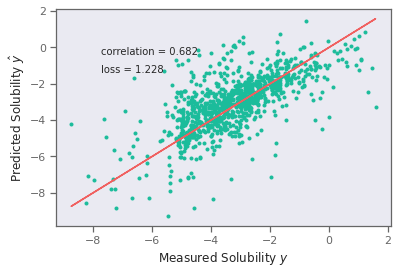
\includegraphics[width=0.8\linewidth]{fig/predict_solubility.png}
    \caption{เปรียบเทียบค่าสภาพการละลายที่ได้จากการทำนายและค่าอ้างอิง}
    \label{fig:pred_solubility}
\end{figure}

\end{enumerate}
 % การเรียนรู้เชิงลึก
% LaTeX source for ``การเรียนรู้ของเครื่องสำหรับเคมีควอนตัม (Machine Learning for Quantum Chemistry)''
% Copyright (c) 2022 รังสิมันต์ เกษแก้ว (Rangsiman Ketkaew).

% License: Creative Commons Attribution-NonCommercial-NoDerivatives 4.0 International (CC BY-NC-ND 4.0)
% https://creativecommons.org/licenses/by-nc-nd/4.0/

\chapter{การเลือกและปรับแต่งโมเดล}
\label{ch:reg_sel_model}

\begin{figure}[htbp]
    \centering
    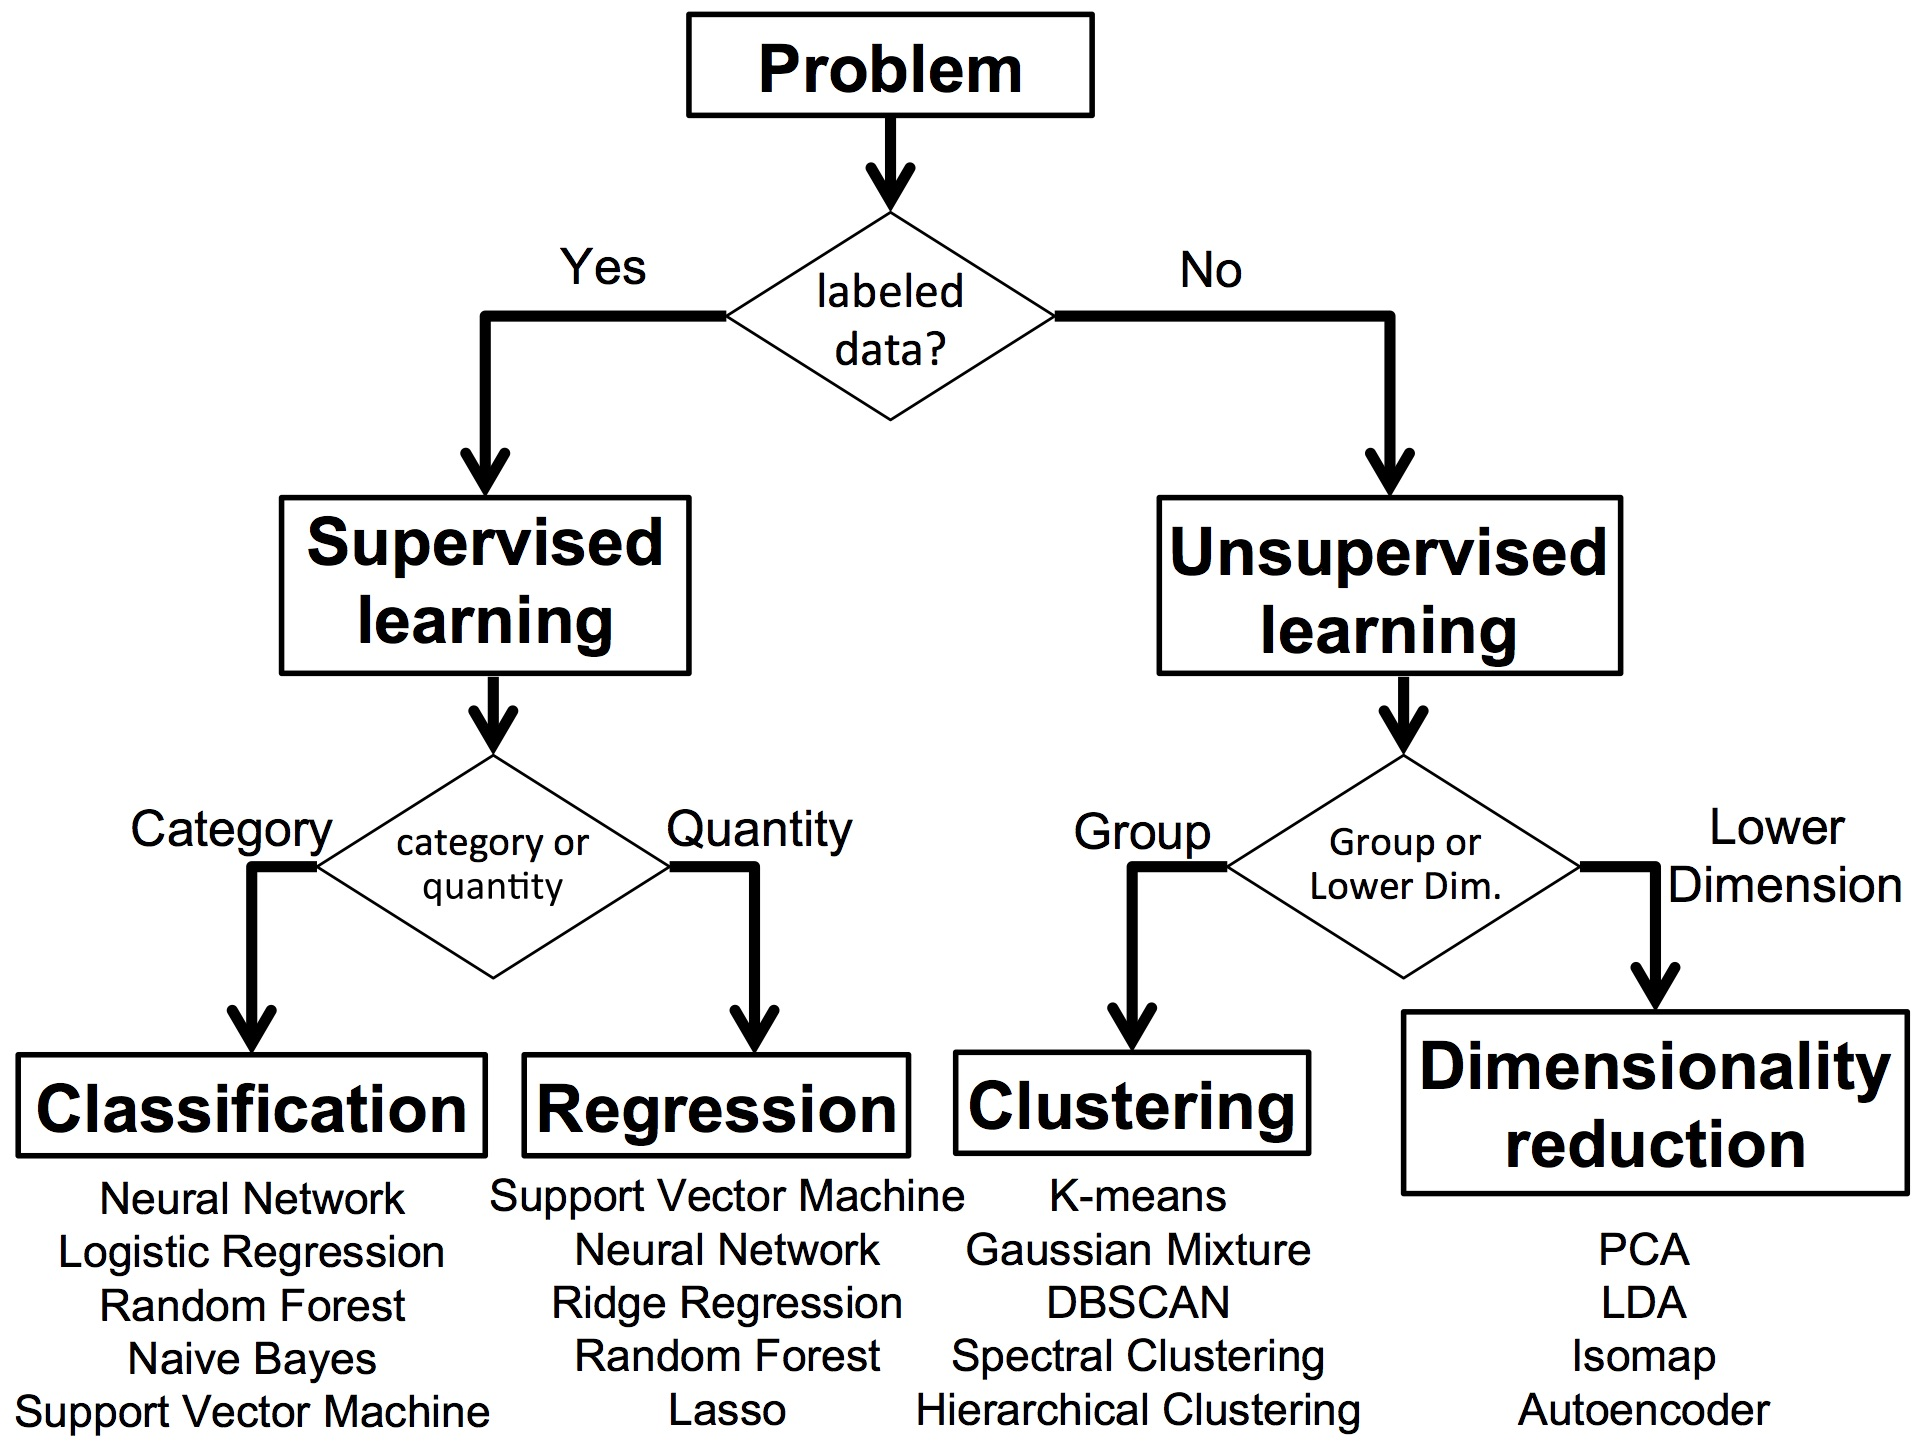
\includegraphics[width=0.9\linewidth]{fig/ml-prediction.jpg}
    \caption{การเลือกโมเดล ML (เครดิตภาพ: https://pythonnumericalmethods.berkeley.edu)}
    \label{fig:ml_prediction}
\end{figure}

การทำให้โมเดลมีความสม่ำเสมอ (Regularization) เพื่อเพิ่มความถูกต้องและการเลือกโมเดล (Model Selection) เป็นสิ่งที่จำเป็นมากใน%
ขั้นตอนของการฝึกสอนโมเดล ในบทนี้เราจะมาดูรายละเอียดและแนวทางในการเลือกอัลกอริทึมสำหรับสร้างโมเดล ML รวมไปถึงเทคนิคการปรับแต่ง%
โมเดลเพื่อให้มีประสิทธิภาพในการทำนายมากที่สุด ตัวอย่างของขั้นตอนการพิจารณาเลือกอัลกอริทึม ML นั้นแสดงตามภาพที่ \ref{fig:ml_prediction}
โดยเริ่มต้นจากปัญหาที่เราต้องการศึกษาก่อน แล้วก็พิจารณาว่าชุดข้อมูลของเรานั้นมี Label หรือคำตอบของแต่ละข้อมูลหรือไม่ ถ้าหากว่ามี Label 
เราก็สามารถใช้อัลกอริทึมแบบ Supervised ML ได้ แต่ถ้าหากไม่มี Label เราก็ไม่มีทางเลือกอื่นนอกจากจะต้องใช้อัลกอริทึมแบบ Unsupervised 
ML เท่านั้น (สำหรับกรณีที่มี Label นั้นเราอาจจะใช้ Unsupervised ML ด้วยก็ได้ โดยแกล้งทำเป็นไม่สนใจ Label) เมื่อเราแบ่งประเภทของ%
โจทย์ปัญหาได้แล้ว ขั้นตอนต่อมาคือการเลือกวิธีในการแก้ปัญหา ซึ่งขั้นตอนนี้ก็จะนำไปสู่การเลือกอัลกอริทึม ML แบบต่าง ๆ นั่นเอง โดยโจทย์ปัญหา%
หลัก ๆ ที่เรามักจะเจอนั้นมีด้วยกัน 4 แบบดังนี้

\begin{enumerate}
    \item Classification (การแบ่งประเภท)
    
    \item Regression (การถดถอย)
    
    \item Clustering (การจัดกลุ่ม)
    
    \item Dimensionality Reduction (การลดมิติของข้อมูล)
\end{enumerate}

โดยโจทย์ปัญหาแต่ละแบบนั้นก็จะมีอัลกอริทึมที่เหมาะสมสำหรับการแก้ปัญหานั้น ๆ เช่น Ridge Regression ก็จะเหมาะสำหรับโจทย์ Regression

%--------------------------
\section{การเลือกโมเดล}
\label{sec:choose_model}
\idxth{การเลือกโมเดลการเรียนรู้ของเครื่อง}
\idxen{Model Selection}
%--------------------------

อัลกอริทึมหรือโมเดล ML แต่ละอันนั้นก็มีข้อดีข้อเสียแตกต่างกันไป ผู้เขียนขอสรุปง่าย ๆ ดังนี้ (เน้นเฉพาะโมเดลที่ได้รับความนิยมในการใช้งาน)

%--------------------------
\subsection{Linear Regression}
\label{ssec:pros_cons_lin_reg}
\idxth{Model Selection!Linear Regression}
%--------------------------

\noindent \textbf{ข้อดี}
\begin{itemize}[topsep=0pt]
    \item สามารถเขียนโค้ดได้ง่าย และฝึกสอนโมเดลได้อย่างมีประสิทธิภาพ
    
    \item ปัญหา Overfitting ของ Linear Regression สามารถแก้ได้ด้วยการทำ Regularization
    
    \item มีประสิทธิภาพมาก ๆ เมื่อชุดข้อมูลสามารถแยกได้เชิงเส้น (Linearly Separable)
\end{itemize}

\noindent \textbf{ข้อด้อย}
\begin{itemize}[topsep=0pt]
    \item ข้อมูลที่อยู่ในชุดข้อมูลที่ใช่สำหรับการฝึกสอนโมเดล Linear Regression นั้นควรจะต้องไม่ขึ้นต่อกัน แต่ทว่าในชีวิตจริงนั้นข้อมูลก็%
    มักจะขึ้นต่อกันเสมอ

    \item สามารถเกิด Noise และ Overfitting ได้ง่าย
    
    \item การที่มี Outlier ในชุดข้อมูลนั้นจะส่งผลให้โมเดลมีประสิทธิภาพที่ต่ำลงมาก ๆ
\end{itemize}

%--------------------------
\subsection{Logistic Regression}
\label{ssec:pros_cons_log_reg}
\idxth{Model Selection!Logistic Regression}
%--------------------------

\noindent \textbf{ข้อดี}
\begin{itemize}[topsep=0pt]
    \item โอกาสเกิด Overfitting น้อย แต่ว่าสามารถเกิด Overfitting ได้ในชุดข้อมูลที่มีจำนวนมิติสูง ๆ
    
    \item มีประสิทธิภาพมาก ๆ เมื่อชุดข้อมูลมี Features ที่สามารถแยกกันได้แบบเชิงเส้น
    
    \item สามารถเขียนโค้ดได้ง่าย และฝึกสอนโมเดลได้อย่างมีประสิทธิภาพ
\end{itemize}

\noindent \textbf{ข้อด้อย}
\begin{itemize}[topsep=0pt]
    \item ไม่ควรใช้อัลกอริทึมนี้สำหรับกรณีที่จำนวน Observation นั้นมีน้อยกว่าจำนวนของ Feature

    \item เหมาะสำหรับชุดข้อมูลที่มีความเป็นเชิงเส้น ซึ่งหาได้ยากในชีวิต (ปกติเรามักจะมีเจอชุดข้อมูลแบบที่ไม่เป็นเชิงเส้น)
    
    \item ใช้ทำนายได้แค่ฟังก์ชันที่ไม่ต่อเนื่อง (Discrete Function)
\end{itemize}

%--------------------------
\subsection{Support Vector Machine}
\label{ssec:pros_cons_svm}
\idxth{Model Selection!Support Vector Machine}
%--------------------------

\noindent \textbf{ข้อดี}
\begin{itemize}[topsep=0pt]
    \item เหมาะสำหรับข้อมูลที่มีจำนวนมิติเยอะ ๆ (High-dimensional Data)
    
    \item สามารถใช้กับชุดข้อมูลที่มีขนาดเล็กได้ (จำนวนข้อมูลไม่เยอะ)
    
    \item สามารถแก้ปัญหาแบบไม่เป็นเชิงเส้นได้ (Non-linear Problem)
\end{itemize}

\noindent \textbf{ข้อด้อย}
\begin{itemize}[topsep=0pt]
    \item ไม่ค่อยมีประสิทธิภาพเมื่อใช้กับชุดข้อมูลที่มีขนาดใหญ่
    
    \item ต้องเลือก Kernel ที่เหมาะสม ถ้าเลือก Kernel ไม่ดีก็จะได้โมเดลที่ไม่มีประสิทธิภาพ
\end{itemize}

%--------------------------
\subsection{Neural Network}
\label{ssec:pros_cons_nn}
\idxth{Model Selection!Neural Network}
%--------------------------

\noindent \textbf{ข้อดี}
\begin{itemize}[topsep=0pt]
    \item มีคุณสมบัติที่ทำให้โมเดลสามารถทำงานต่อไปได้แม้จะเกิด Failure ขึ้น เรียกง่าย ๆ ว่า ทนทานต่อความเสียหายมี Fault Tolerance
    
    \item มีความสามารถในการเรียนรู้โมเดลที่เป็นแบบไม่เชิงเส้นและความสัมพันธ์ระหว่างตัวแปรที่มีความซับซ้อน
    
    \item สามารถ Generalize บนชุดข้อมูลที่ไม่เคยเห็นมาก่อนได้ (Unseen Data)
\end{itemize}

\noindent \textbf{ข้อด้อย}
\begin{itemize}[topsep=0pt]
    \item ใช้ระยะเวลาในการฝึกสอนโมเดลนาน
    
    \item ไม่การันตีว่าการฝึกสอนโมเดลจะลู่เข้า (Non-gauranteed Convergence)
    
    \item ตีความโมเดลได้ยาก เช่น เราไม่สามารถบอกความสัมพันธ์ระหว่างโหนดใน Hidden Layer ได้ ซึ่งเราเรียกว่าโมเดลแบบนี้ว่า Black 
    Box 

    \item ประสิทธิภาพในการฝึกสอนโมเดลขึ้นอยู่กับประสิทธิภาพของของเครื่องที่ใช้รันด้วย (Hardware)
    
    \item ไม่เหมาะสำหรับผู้เริ่มต้นศึกษา ML เพราะว่าต้องใช้ประสิทธิภาพและความสามารถในการนำไปจัดการปัญหาและปรับแก้โมเดลเพื่อทำให้%
    เรียนรู้ได้ดียิ่งขึ้น
\end{itemize}

%--------------------------
\subsection{Printipal Component Analysis}
\label{ssec:pros_cons_pca}
\idxth{Model Selection!Printipal Component Analysis}
%--------------------------

\noindent \textbf{ข้อดี}
\begin{itemize}[topsep=0pt]
    \item สามารถลดความซับซ้อนของความสัมพันธ์ระหว่าง Feature ได้
    
    \item สามารถลดปัญหา Overfitting
\end{itemize}

\noindent \textbf{ข้อด้อย}
\begin{itemize}[topsep=0pt]
    \item องค์ประกอบหลัก (Principal Component) นั้นวิเคราะห์และตีความได้ยาก
    
    \item การใช้วิธีนี้ทำให้เราสูญเสียข้อมูล (ความสัมพันธ์ระหว่าง Feature) หรือ Information Loss
    
    \item จำเป็นจะต้องทำการ Standardize ชุดข้อมูลก่อน
\end{itemize}

%--------------------------
\subsection{K Means Clustering}
\label{ssec:pros_cons_kmeans}
\idxth{Model Selection!K Means Clustering}
%--------------------------

\noindent \textbf{ข้อดี}
\begin{itemize}[topsep=0pt]
    \item สามารถเขียนโค้ดได้ง่าย ไม่ซับซ้อน
    
    \item สามารถนำไปใช้กับชุดข้อมูลที่มีขนาดใหญ่มาก ๆ ได้
    
    \item การันตีว่าการฝึกสอนโมเดลนั้นลู่เข้าแน่นอน
    
    \item สามารถปรับให้เข้ากับชุดข้อมูลใหม่ได้ง่าย ๆ
\end{itemize}

\noindent \textbf{ข้อด้อย}
\begin{itemize}[topsep=0pt]
    \item ไม่เหมาะสำหรับชุดข้อมูลที่มี Outlier
    
    \item การเลือกค่า $K$ สำหรับ Clustering นั้นค่อนข้างยุ่งยาก
    
    \item ประสิทธิภาพของโมเดลขึ้นอยู่กับพารามิเตอร์เริ่มต้น
    
    \item ความสามารถในการ Scale นั้นจะลดลงเมื่อจำนวนมิติเพิ่มขึ้น
\end{itemize}

%--------------------------
\subsection{K Nearest Neighbor}
\label{ssec:pros_cons_knn}
\idxth{Model Selection!K Nearest Neighbor}
%--------------------------

\noindent \textbf{ข้อดี}
\begin{itemize}[topsep=0pt]
    \item สามารถทำนายได้โดยไม่ต้องฝึกสอนโมเดล
    
    \item เป็นวิธีที่สิ้นเปลืองน้อยมาก โดยมี Time Complexity เท่ากับ $\mathcal{O}(n)$
    
    \item สามารถนำไปใช้ได้กับโจทย์ Regression และ Classification
\end{itemize}

\noindent \textbf{ข้อด้อย}
\begin{itemize}[topsep=0pt]
    \item ไม่เหมาะสำหรับชุดข้อมูลขนาดใหญ่
    
    \item ไม่เหมาะสำหรับชุดข้อมูลที่มี Noise เยอะมากเกินไป และข้อมูลไม่ครบ รวมไปถึง Outlier ด้วย 
    
    \item จำเป็นต้องมีการทำ Feature Scaling
    
    \item การเลือกค่า $K$ นั้นค่อนข้างยุ่งยาก
\end{itemize}

%--------------------------
\subsection{Machine Learning Trade-off}
\label{ssec:ml_trade_off}
\idxth{Model Selection!Model Trade-off}
%--------------------------

\begin{figure}[H]
    \centering
    \includegraphics[width=0.9\linewidth,page=2]{fig/ml-trade-off.jpg}
    \caption{เปรียบเทียบอัลกอริทึม ML แบบต่าง ๆ ตามความสัมพันธ์ระหว่างประสิทธิภาพของโมเดลกับการตีความโมเดล}
    \label{fig:ml_traide}
\end{figure}

นอกจากนี้ยังมีสิ่งที่เราจะต้องให้ความสำคัญในการเลือกโมเดล ML ด้วยนั่นก็คือความถูกต้องในการทำนายหรือประสิทธิภาพของโมเดล (Accuracy) 
กับการที่เราสามารถตีความโมเดลนั้น ๆ ได้ (Interpretability หรือ Exaplainability) โดยจากภาพที่ \ref{fig:ml_traide} จะเห็นได้%
ว่าโมเดล Neural Network นั้นมีประสิทธิภาพในการทำนายที่สูงมาก (ทำนายได้ถูกต้อง) เมื่อเทียบกับโมเดล ML อื่น ๆ เช่น Linear Regression 
ซึ่งมีความสามารถที่น้อยกว่า แต่ถ้าหากเรามาดูที่ Explainability แล้วจะพบว่าจะตรงข้ามกับ Accuracy เลย ซึ่งโมเดล Linear Regression 
นั้นสามารถนำมาตีความและอธิบายถึงสิ่งกระบวนที่เกิดขึ้นในโมเดลได้ดีกว่า เช่น สามารถอธิบายความสัมพันธ์ระหว่างอินพุตและเอาต์พุตได้ดีกว่าโมเดล 
Neural Network ดังนั้นการที่เราจะต้องตัดสินใจเลือกใช้โมเดลสักโมเดลเพื่อมาใช้แก้ปัญหาโจทย์ของเรานั้นเราควรจะต้องพิจารณาทั้งสองปัจจัยนี้เป็นหลัก
ซึ่งเราเรียกกระบวนการแบบนี้ว่าเป็นการชั่งน้ำหนักสำหรับการตัดสินใจหรือ Trade-off นั่นเอง

ถ้าหากถามว่าทำไมการตีความโมเดลได้นั้นถึงสำคัญ นั่นก็เพราะว่าบ่อยครั้งที่เราต้องการวิเคราะห์ข้อมูลในลักษณะสามารถใช้พิจารณาผลกระทบและ%
ความสำคัญของคุณสมบัติต่าง ๆ ได้อย่างตรงไปตรงมา โดยโมเดลที่ตีความได้ (Interpretable Model) นั้นไม่ว่าจะเป็นโมเดลอยู่ในรูปแบบของ%
สมการ เช่น โมเดลจำพวก Regression ที่เราสามารถนำค่าสัมประสิทธิ์ของตัวแปรในสมการต่าง ๆ มาอธิบายผลกระทบที่ตัวแปรมีแก่ผลลัพธ์ที่ต้องการ%
ทำนาย หรือ โมเดลจำพวกต้นไม้ตัดสินใจ (Decision Tree) ซึ่งหลังจากการฝึกฝนโมเดลแล้วนั้น เราสามารถศึกษากฎการตัดสินใจในขั้นต่าง ๆ 
เพื่อจำแนกผลลัพธ์ที่ต้องการได้

%--------------------------
\section{Cross Validation}
\label{sec:cross_val}
\idxboth{การทดสอบแบบข้าม}{Cross Validation}
%--------------------------

วิธีการตรวจสอบโมเดลวิธีแรกนี้เป็นวิธีที่ได้รับความนิยมเป็นอย่างมากเพราะว่าสามารถทำได้ง่ายและให้ผลลัพธ์ที่น่าเชื่อถือ นั่นก็คือ 
\enquote{K-Fold Cross Validation} หรือเรียกสั้น ๆ ว่า Cross Validation วิธีนี้เริ่มด้วยการแบ่งข้อมูล $k$ ให้มีขนาดของแต่ละส่วนเท่า ๆ กัน 
หลังจากนั้นทำเก็บข้อมูลหนึ่งส่วนไว้ใช้สำหรับเป็นตัวทดสอบโมเดลนั่นก็คือการทำ Validation แล้วทําวนไปเช่นนี้จนครบจํานวนที่แบ่งไว้ เช่น 
การทดสอบด้วยวิธี 5-fold Cross Validation ในรอบแรกเราจะทำการเทรนโมเดลด้วยชุดข้อมูลที่เกิดจากการวมส่วนที่ 2, 3, 4, และ 5 
และทำการทดสอบด้วยข้อมูลส่วนที่ 1 และในรอบที่สองเราจะเปลี่ยนมาเทรนโมเดลด้วยข้อมูลของส่วนที่ 1, 3, 4, และ 5 แล้วนำโมเดลมาทดสอบ%
ด้วยข้อมูลส่วนที่ 2

จริง ๆ แล้วมีวิธีการทำ Cross Validation หลากหลายวิธีมาก โดยมีภาพประกอบโค้ดที่เขียนด้วยภาษา Python และใช้ไลบรารี่ Scikit-learn 
สำหรับ Cross Validation แต่ละแบบดังนี้

%--------------------------
\subsection{Train Test Split}
\label{ssec:train_test_split}
\idxen{Cross Validation!Train Test Split}
%--------------------------

ฟังก์ชัน \pyinline{train_test_split} จะทำการแบ่ง Array หรือ Matrices ออกเป็น Train กับ Test Set แบบสุ่ม

\begin{figure}[H]
    \centering
    \includegraphics[width=0.9\linewidth,page=1]{fig/cross_validation.pdf}
    \caption{การทำ Cross Validation ด้วย \pyinline{train_test_split}}
    \label{fig:train_test_split}
\end{figure}

\begin{lstlisting}[style=MyPython]
import numpy as np
from sklearn.model_selection import train_test_split

X = np.array([[0, 1], [2, 3], [4, 5], [6, 7], [8, 9]])
y = np.array([0, 1, 2, 3, 4])
X_train, X_test, y_train, y_test = train_test_split(
    X, y, test_size=0.33, random_state=42)
\end{lstlisting}

%--------------------------
\subsection{Cross Val Score}
\label{ssec:cross_val_score}
\idxen{Cross Validation!Cross Val Score}
%--------------------------

ฟังก์ชัน \pyinline{cross_val_score} ทำการคำนวณคะแนน (Score) โดยการทำ Cross Validation และแสดงค่า Score ของแต่ละส่วน

\begin{figure}[H]
    \centering
    \includegraphics[width=0.9\linewidth,page=2]{fig/cross_validation.pdf}
    \caption{การทำ Cross Validation ด้วย \pyinline{cross_val_score}}
    \label{fig:cross_val_score}
\end{figure}

\begin{lstlisting}[style=MyPython]
from sklearn.model_selection import cross_val_score
from sklearn.datasets import load_iris

iris = load.iris()
clf = svm.SVC(kernel="linear", C=1)
scores = cross_val_score(clf, iris.data, iris.target, cv=5)
\end{lstlisting}

%--------------------------
\subsection{Cross Val Predict}
\label{ssec:cross_val_predict}
\idxen{Cross Validation!Cross Val Score}
%--------------------------

ฟังก์ชัน \pyinline{cross_val_predict} ทำการทำนายสมาชิกหรือข้อมูลแต่ละตัวที่อยู่ใน Test Set

\begin{figure}[H]
    \centering
    \includegraphics[width=0.9\linewidth,page=3]{fig/cross_validation.pdf}
    \caption{การทำ Cross Validation ด้วย \pyinline{cross_val_predict}}
    \label{fig:cross_val_predict}
\end{figure}

\begin{lstlisting}[style=MyPython]
from sklearn.model_selection import cross_val_predict
from sklearn.datasets import load_iris

iris = load.iris()
clf = svm.SVC(kernel="linear", C=1)
predicted = cross_val_predict(clf, iris.data, iris.target, cv=10)
\end{lstlisting}

%--------------------------
\subsection{K Fold}
\label{ssec:f_fold}
\idxen{Cross Validation!K Fold}
%--------------------------

ฟังก์ชัน \pyinline{KFold} จะทำการแบ่ง Dataset ออกเป็น K Fold (โดยที่ K คือจำนวนของการแบ่ง เช่น 3) โดยไม่มีการสลับข้อมูล 
โดยที่แต่ละ Fold จะถูกนำมาใช้เป็น Validation

\begin{figure}[H]
    \centering
    \includegraphics[width=0.9\linewidth,page=4]{fig/cross_validation.pdf}
    \caption{การทำ Cross Validation ด้วย \pyinline{KFold}}
    \label{fig:f_fold}
\end{figure}

\begin{lstlisting}[style=MyPython]
import numpy as np
from sklearn.model_selection import KFold

X = np.array([[1, 2], [3, 4], [1, 2], [3, 4]])
y = np.array([1, 2, 3, 4])
kf = KFold(n_splits=2)
kf.split(X)
kf.get_n_splits(X) # OUTPUT = 2

for i, (train_index, test_index) in enumerate(kf.split(X)):
    print(f"Fold {i}:")
    print(f"  Train: index={train_index}")
    print(f"  Test:  index={test_index}")
\end{lstlisting}

%--------------------------
\subsection{Leave One Out}
\label{ssec:leave_one_out}
\idxen{Cross Validation!Leave One Out}
%--------------------------

ฟังก์ชัน \pyinline{LeaveOneOut} เป็นการนำข้อมูลแต่ละตัวมาใช้เป็น Test Set 1 ครั้งหรือเรียกว่า Singleton ซึ่งจริง ๆ แล้ว 
\pyinline{LeaveOneOut()} นั้นจะเหมือนกับการใช้ \pyinline{KFold(n_splits=n)} และ \pyinline{LeavePOut(p=1)} โดยที่ 
\pyinline{n} คือจำนวนของข้อมูลหรือ Sample

\begin{figure}[H]
    \centering
    \includegraphics[width=0.9\linewidth,page=5]{fig/cross_validation.pdf}
    \caption{การทำ Cross Validation ด้วย \pyinline{LeaveOneOut}}
    \label{fig:leave_one_out}
\end{figure}

\begin{lstlisting}[style=MyPython]
import numpy as np
from sklearn.model_selection import LeaveOneOut

X = np.array([[1, 2], [3, 4]])
y = np.array([1, 2])
loo = LeaveOneOut()
loo.get_n_splits(X) # OUTPUT = 2 

for i, (train_index, test_index) in enumerate(loo.split(X)):
    print(f"Fold {i}:")
    print(f"  Train: index={train_index}")
    print(f"  Test:  index={test_index}")
\end{lstlisting}

%--------------------------
\subsection{Leave P Out}
\label{ssec:leave_p_out}
\idxen{Cross Validation!Leave P Out}
%--------------------------

ฟังก์ชัน \pyinline{LeavePOut} นั้นคล้ายกับ \pyinline{LeaveOneOut()} มาก แต่จะมีความแตกต่างกันตรงที่วิธีนี้นั้นสามารถกำหนดจำนวน%
ของข้อมูลหรือ Sample ที่เรานำไปไปใช้เป็น Test Set ได้

\begin{figure}[H]
    \centering
    \includegraphics[width=0.9\linewidth,page=6]{fig/cross_validation.pdf}
    \caption{การทำ Cross Validation ด้วย \pyinline{LeavePOut}}
    \label{fig:leave_p_out}
\end{figure}

\begin{lstlisting}[style=MyPython]
import numpy as np
from sklearn.model_selection import LeavePOut

X = np.array([[1, 2], [3, 4], [5, 6], [7, 8]])
y = np.array([1, 2, 3, 4])
lpo = LeavePOut(2)
lpo.get_n_splits(X) # OUTPUT = 6

for i, (train_index, test_index) in enumerate(lpo.split(X)):
    print(f"Fold {i}:")
    print(f"  Train: index={train_index}")
    print(f"  Test:  index={test_index}")
\end{lstlisting}

%--------------------------
\section{การคัดเลือกลักษณะเฉพาะ}
\label{sec:select_feat}
\idxen{Feature Selection}
%--------------------------

\begin{algorithm}[ht]
    \caption{อัลกอริทึม Forward Search สำหรับการทำ Feature Selection}
    \label{alg:forward_search}
    \begin{algorithmic}
    \State Initialize $\mathcal{F} = \emptyset$.
    \Repeat
        \For{$i=1,\ldots,d$}
            \If{$i \not\in \mathcal{F}$}
                \State $\mathcal{F}_i = \mathcal{F} \cup \{i\}$
                \State Use some version of cross validation to evaluate features $\mathcal{F}_i$.
                \State (i.e., train your learning algorithm using only the features in $\mathcal{F}_i$, and 
                estimate its generalization error.)
            \EndIf
        \EndFor
        \State Set $\mathcal{F}$ to be the best feature subset found in the previous step. % DIFF.
    \Until{convergence}
    \State Select and output the best feature subset that was evaluated during the entire search procedure.
    \end{algorithmic}
\end{algorithm}

การคัดเลือกลักษณะเฉพาะ (Feature Selection) เป็นการหา Feature ที่เหมาะสมที่สุดสำหรับการใช้อธิบายข้อมูลของโมเลกุล โดยเราจะทำการ%
เรียงลำดับความสำคัญของ Feature แล้วทำการคัดเลือกเฉพาะ Feature ที่คิดว่าสอดคล้องกับเอาต์พุตที่ต้องการทำนายและคัด Feature ที่มีความ%
สำคัญน้อยออกไปเพื่อหลีกเลี่ยง Bias ที่อาจจะเกิดขึ้น อธิบายง่าย ๆ คือเป็นเทคนิคที่เรานำมาใช้เพื่อลดจำนวณของ Feature นั่นเอง 

อัลกอริทึมของ Feature Selection แบบที่ง่ายที่สุดนั้นชื่อว่า Forward Search ซึ่งดูได้ตามอัลกอริทึมที่ \ref{alg:forward_search} โดยเริ่ม%
ต้นนั้นกำหนดให้ $\mathcal{F}$ เป็นเซตของจำนวน Feature ทั้งหมดซึ่งยังเป็นเซตว่างอยู่ แล้วเราก็ทำการ Cross Validation ไปทีละ Feature
โดยในลูปด้านในนั้นจะเพิ่ม Feature เข้าไปใน $\mathcal{F}$ ทีละอันจนกระทั้งครบทุก Feature $\mathcal{F} = \{1,\ldots ,d\}$ 
ซึ่งจะเป็นการสิ้นสุดกระบวนการทำ Feature Search 

นอกจากนี้ยังมีอัลกอริทึมที่ตรงข้ามกับ Forward Search เรียกว่า Backward Search โดยแทนที่เราจะกำหนด $\mathcal{F}$ ให้เป็นเซตว่างนั้น%
เราจะเริ่มด้วย $\mathcal{F}$ ที่เป็นเซตที่มี Feature อยู่ครบทั้งหมดแล้วทำการลบ Feature ออกทีละอันจนกระทั่ง $\mathcal{F}$ เป็นเซตว่าง

%--------------------------
\section{ปัญหา Bias-Variance}
\label{sec:bias_var_prob}
\idxen{Bias-Variance}
%--------------------------

หนึ่งในปัญหาที่เราทุกคนจะต้องเจอในการสร้างโมเดลนั่นก็คือ Bias-Variance Problem ซึ่งนำไปสู่ปัญหาเรื่อง Overfitting ต่อไป
เราลองมาดูรายละเอียดกันครับ กำหนดให้โมเดลของเราแทนด้วย $\hat{f}(\vec{x})$ และค่าอ้างอิงหรือคำตอบที่เราจะมาเทียบกับการทำนายเป็น 
$y$ และความคลาดเคลื่อนที่เกิดขึ้นเป็น

\begin{equation}
    E\left[\left(y - \hat{f}(\vec{x})\right)^2\right]
\end{equation}

ซึ่งจริง ๆ แล้ว เป็นฟังก์ชันที่สมบูรณ์แบบมาก แต่ทว่าในความเป็นจริงแล้วในชุดข้อมูลของเรานั้นย่อมมี Noise $(\epsilon)$ ซึ่งค่าความแตกต่าง%
ระหว่างโมเดลของเรากับคำตอบก็จะมีการปนเปื้อนหรือ Contaminate โดย $\epsilon$ ดังนี้

\begin{equation}
    y = f(\vec{x}) + \epsilon
\end{equation}

\noindent จึงทำให้ค่าความคลาดเคลื่อนที่เกิดขึ้นจริง ๆ นั้นมีสมการดังต่อไปนี้ 

\begin{align}
    E\left[\left(y - \hat{f}(\vec{x})\right)^2\right] &= 
    E\left[y^2\right] + E\left[\hat{f}(\vec{x})^2\right] - 2 E\left[y\hat{f}(\vec{x})\right] \\
    &= E\left[\left(f(\vec{x}) - \epsilon\right)^2\right] + \hat{f}(\vec{x})^2 - 2 E\left[\left(f(\vec{x}) - 
    \epsilon\right)\right]\hat{f}(\vec{x})
\end{align}

\noindent ซึ่งถ้าหากเราทำการพิสูจน์สมการด้านบนโดยพยายามจัดรูปให้อยู่ในเทอมที่มี Bias และ Variance จากชุดข้อมูล เราจะได้สมการดังต่อไปนี้

\begin{align}\label{eq:bias_variance}
E\left[\left(y - \hat{f}(\vec{x})\right)^2\right] = 
    & \underbrace{E\left[f(\vec{x}) - \hat{f}\left(\vec{x}; \bm{D}\right)\right]^2}_{\text{Bias}} \nonumber \\
    & + \underbrace{E\left[\left(E\left[\hat{f}\left(\vec{x}; \bm{D}\right)\right] - 
    \hat{f}\left(\vec{x}; \bm{D}\right)\right)^2\right]}_{\text{Variance}} \nonumber \\
    & + \sigma^2
\end{align}

โดยพจน์แรกนั้นเป็น Bias, พจน์ที่สองเป็น Variance และพจน์ที่สามเป็นค่าความแปรปรวนที่คำนวณจาก Standard Deviation ของ Noise 
$(\epsilon)$ ประเด็นก็คือว่าเราสามารถควบคุม Bias กับ Variance ได้ แต่เราไม่สามารถควบคุม Noise ได้เพราะมันเป็นสิ่งที่ผูกติดมากับชุด%
ข้อมูล ซึ่งการที่เรามี Bias และ Variance ที่ไม่สมดุลกันนั้นจะทำให้เกิดผลลัพธ์ที่ตามมาในระหว่างการฝึกสอนโมเดล นั่นคือ Overfitting และ 
Underfitting

%--------------------------
\section{การเพิ่มประสิทธิภาพการเรียนรู้และแก้ปัญหา Overfitting}
\label{sec:fix_overfit}
%--------------------------

\begin{figure}[htbp]
    \centering
    \includegraphics[width=\linewidth]{fig/overfitting.png}
    \caption{โมเดลที่มีความ Overfitting และ Underfitting กับชุดข้อมูลมากเกินไป}
    \label{fig:overfitting}
\end{figure}

\begin{description}[style=nextline]
    \item[Overfitting] โมเดลตอบสนองต่อ Noise ที่มากเกินไป ทำให้เกิดการเรียนรู้และจดจำ Noise และไม่สามารถที่จะเรียนรู้รายละเอียด%
    จริง ๆ ของข้อมูลได้ ซึ่งส่งผลให้ทำนายข้อมูลไม่ได้หรือผิดพลาดมากกว่าที่คาดไว้หรือยอมรับได้ โดยกรณีนี้โมเดลจะมีค่าความแปรปรวนของข้อมูลสูง 
    (High Variance)
    
    \item[Underfitting] โมเดลของเราไม่สามารถหาความสัมพันธ์ระหว่างอินพุต $(x)$ กับเอาต์พุต $(y)$ ได้เพราะว่ามีข้อมูลที่ใช้ใน%
    การเทรนน้อยเกินไปหรือดึงข้อมูลออกมาจาก Training Set ได้ไม่เพียงพอที่จะเรียนรู้ โดยในกรณีนี้โมเดลจะมีค่าความเอนเอียงสูง (High Bias)

    \item[Noisy] โมเดลไม่มี Overfitting และ Underfitting แต่ยังมีค่า Error ของการฝึกสอนที่ยังสูงอยู่มาก ซึ่งสาเหตุก็อาจจะมาจาก%
    การที่ชุดข้อมูลมี Noise มากเกินไปนั่นเอง
\end{description}

ภาพที่ \ref{fig:overfitting} แสดงการเปรียบเทียบระหว่างกรณีของ Underfitting และ Overfitting ซึ่งเป็นหนึ่งในปัญหาหลักที่มักจะพบ%
เจอได้ทั่วไปใน ML โดยเราสามารถสรุปความสัมพันธ์จากกรณีได้กล่าวได้ดังนี้

\fbox{%
\begin{minipage}{0.9\linewidth}
    \begin{align*}
        \text{Bias สูง} &\;\longleftrightarrow\; \text{Underfitting}\\
        \text{Variance สูง} &\;\longleftrightarrow\; \text{Overfitting}\\
        \text{$\sigma^2$ มาก} &\;\longleftrightarrow\; \text{Noisy Data}\\
    \end{align*}
\end{minipage}}

วิธีการจัดการกับ Overfitting แบบที่ง่ายที่สุดคือการเพิ่มจำนวนข้อมูลในการฝึกสอนโมเดล นอกจากนี้ยังมีวิธีอื่น ๆ ที่เราสามารถใช้ในการจัดการกับ%
ปัญหาข้างต้นได้เช่นเดียวกัน มีดังต่อไปนี้

%--------------------------
\subsection{Data Augmentation}
\label{ssec:data_aug}
\idxen{Data Augmentation}
%--------------------------

\begin{figure}[H]
    \centering
    \includegraphics[width=0.9\linewidth]{fig/data_aug_butterfly.jpg}
    \caption{ตัวอย่างการทำ Data Augmentation สำหรับข้อมูลที่เป็นรูปภาพ เช่น การเปลี่ยนสี การเพิ่มความคมชัด การเพิ่ม Noise 
    (เครดิตภาพ: \textit{PLoS ONE} 12(8): e0183838)}
    \label{fig:data_aug_butterfly}
\end{figure}

วิธีการทำ Data Augmentation นั้นจะตรงข้ามกับการทำความสะอาดข้อมูล (Data Cleaning) นั่นก็คือจะเป็นวิธีที่เราจะใส่ Noise หรือสิ่งที่%
ไม่ได้เกี่ยวข้องกับข้อมูลโดยตรงเข้าไปในชุดการฝึกสอน รวมไปถึงการแก้ไขข้อมูลให้แตกต่างไปจากเดิม แต่ยังคงไว้ซึ่งลักษณะของข้อมูลนั้น 
ซึ่งการทำ Data Augmentation จะเป็นการช่วยไม่ใช่ให้เกิดการเรียนรู้ที่มันยึดติดกับชุดข้อมูลฝึกสอนมากเกินไป ในปัจจุบันวิธีการนี้ได้รับความนิยม%
เพราะสามารถทำได้ง่าย สะดวก และไม่มีความซับซ้อนในการทำ โดยมีความจำเป็นอย่างยิ่งกรณีที่ชุดข้อมูลมีขนาดเล็ก (จำนวนข้อมูลไม่เยอะ) 
แต่ต้องการนำมาใช้ในการฝึกสอนด้วยเทคนิค ML ที่ต้องการข้อมูลในปริมาณที่เยอะในการฝึกสอน เช่น Deep Learning\autocite{bengio2021}

%--------------------------
\subsection{Early Stopping}
\label{ssec:early_stop}
\idxen{Early Stopping}
%--------------------------

\begin{figure}[H]
    \centering
    \includegraphics[width=0.9\linewidth]{fig/early_stopping.png}
    \caption{การทำ Regularization ด้วยวิธี Early Stopping สำหรับการฝึกสอนโมเดล High-degree Polynomial Regression 
    โดยใช้ Batch Gradient Descent และใช้ RMSE ในการวัดค่าความคลาดเคลื่อน (เครดิตภาพ: https://www.oreilly.com)}
    \label{fig:early_stopping}
\end{figure}

วิธี Early Stopping มีความหมายวิธีการทำงานตามชื่อเลยนั่นก็คือหยุดให้เร็วขึ้น เป็นวิธีการที่เราจะกำหนด (บังคับ) ให้การฝึกสอนหรือ Training 
นั้นหยุดก่อนที่โมเดลของเราจะเริ่มเรียนรู้ Noise ที่อยู่ภายในชุดข้อมูล แทนที่จะเรียนรู้เฉพาะชุดข้อมูลอย่างเดียว ซึ่งวิธีการนี้จะเป็นการป้องกันการเปิด 
Bias แบบตรงไปตรงมา อย่างไรก็ตามเราควรจะต้องระมัดระวังในการใช้เทคนิค Early Stopping เพราะว่าถ้าเราบังคับให้โมเดลหยุดเรียนรู้เร็วเกินไป
ปัญหาที่อาจจะเกิดขึ้นแทนการ Overfitting นั่นก็คือการ Underfitting ของโมเดล ซึ่งการเลือกจุดที่จะให้โมเดลนั้นหยุดการเรียนรู้ก็ถือว่ามีความ%
เป็น Art อย่างหนึ่ง ซึ่งจุดที่เราเลือกต้องมีความเหมาะสมระหว่าง Overfitting และ Underfitting

\noindent โค้ดของการทำ Early Stopping โดยใช้ไลบรารี่ Scikit-Learn

\begin{lstlisting}[style=MyPython]
from copy import deepcopy
from sklearn.metrics import mean_squared_error
from sklearn.preprocessing import StandardScaler

X_train, y_train, X_valid, y_valid = [...]  # split the quadratic dataset

preprocessing = make_pipeline(PolynomialFeatures(degree=90, include_bias=False),
                              StandardScaler())
X_train_prep = preprocessing.fit_transform(X_train)
X_valid_prep = preprocessing.transform(X_valid)
sgd_reg = SGDRegressor(penalty=None, eta0=0.002, random_state=42)
n_epochs = 500
best_valid_rmse = float('inf')

# Training with applying early stopping
for epoch in range(n_epochs):
    sgd_reg.partial_fit(X_train_prep, y_train)
    y_valid_predict = sgd_reg.predict(X_valid_prep)
    val_error = mean_squared_error(y_valid, y_valid_predict, squared=False)
    if val_error < best_valid_rmse:
        best_valid_rmse = val_error
        best_model = deepcopy(sgd_reg)
\end{lstlisting}

\noindent โค้ดของการสร้าง Callback ของ Early Stopping โดยใช้ไลบรารี่ TensorFlow 

\begin{lstlisting}[style=MyPython]
import tensorflow as tf

callback = tf.keras.callbacks.EarlyStopping(monitor='loss', patience=3)

model = tf.keras.models.Sequential([tf.keras.layers.Dense(10)])
model.compile(tf.keras.optimizers.SGD(), loss='mse')

history = model.fit(np.arange(100).reshape(5, 20), np.zeros(5),
                    epochs=10, batch_size=1, callbacks=[callback],
                    verbose=0)

len(history.history['loss'])  # Only 4 epochs are run.
4
\end{lstlisting}

\noindent โดย Callback จะทำการหยุดการฝึกสอน (Training) เมื่อค่า Loss ไม่มีการลดลงภายใน 3 Epochs ที่ต่อเนื่องกัน

%--------------------------
\subsection{Ensemble Method}
\label{ssec:ensemble_model}
\idxen{Ensemble Method}
%--------------------------

\begin{figure}[htbp]
    \centering
    \includegraphics[width=0.9\linewidth]{fig/ensemble_method.png}
    \caption{การทำงานร่วมกันของโมเดลหลาย ๆ โมเดลโดยใช้วิธี Ensemble (เครดิตภาพ: https://www.manning.com)}
    \label{fig:ensemble_method}
\end{figure}

เทคนิคนี้เป็นการนำโมเดลหลาย ๆ โมเดลมารวมกันเพื่อที่จะทำให้ผลลัพธ์ของการทำนายคำตอบมีค่าที่ดีที่สุด โดยโมเดล ML ที่เราจะมานำผสมกันนั้น%
จะเป็นอะไรก็ได้ เช่น Linear Regression, Logistic Regression, Gaussian Process Regression ผู้อ่านสามารถดูภาพที่ 
\ref{fig:ensemble_method} ประกอบได้ โดยจะเห็นว่าเรามีโมเดลที่มีประสิทธิภาพไม่ค่อยดีนักหลาย ๆ โมเดล เราสามารถนำโมเดลเหล่านี้มา%
รวมกันเพื่อให้ได้โมเดลที่มีประสิทธิมากขึ้นได้

โดยเทคนิคย่อยของEnsemble Method ที่นิยมใช้กันนั้นมีอยู่ด้วยกัน 3 วิธี ดังนี้

\begin{itemize}[topsep=0pt]
    \item \textbf{Bagging} เราจะทำการสร้างข้อมูลประเภทเดียวกันแบบหลาย ๆ ชุด แล้วทำการทดสอบกับข้อมูลเพียงแค่บางส่วน (Subset) 
    ของชุดข้อมูล จากนั้นนำผลการทำนายของโมเดลต่าง ๆ มารวมกัน ตัวอย่างของอัลกอริทึมที่ใช้ในการเรียนรู้สำหรับเทคนิค Bagging นี้ เช่น 
    Decision Tree, Random Forest และ Extra Tree
    \idxen{Ensemble Method!Bagging}

    \item \textbf{Boosting} จะทำคล้ายกับ Bagging เลยก็คือเริ่มต้นด้วยการสร้างข้อมูลประเภทเดียวกันแบบหลาย ๆ ชุด แล้วทำการทดสอบ%
    กับข้อมูลชุดเดียวกันโดยทำการทดสอบแบบวนซ้ำ (Iteration) แล้วปรับค่าน้ำหนักเพื่อทำให้ผลการทำนายของโมเดลนั้นดีขึ้นเรื่อย ๆ ซึ่งวิธีนี้ค่อน%
    ข้างเป็นที่นิยมเพราะมีความยืดหยุ่นและใช้ได้กับทุกอัลกอริทึม นอกจากนี้ยังสามารถปรับลดค่าความคลาดเคลื่อนของ Bias ของโมเดลได้ดีอีกด้งบ 
    ตัวอย่างของอัลกอริทึมที่ใช้ในการเรียนรู้สำหรับเทคนิค Boosting นี้ เช่น AdaBoost และ Stochastic Gradient Boosting
    \idxen{Ensemble Method!Boosting}

    \item \textbf{Voting} เราจะเริ่มด้วยการสร้างโมเดลที่แตกต่างกันหลาย ๆ โมเดล เช่น Decision Tree, Support Vector Machine, 
    K-Nearest Neighbors จากนั้นทำการฝึกสอนโมเดลด้วยชุดข้อมูลชุดเดียวกันเพื่อดูผลการทำนายที่ดีที่สุดของแต่ละโมเดล แล้วใช้การโหวตผลที่%
    เหมือนกันหรือคล้ายกันเพื่อเป็นคำตอบสุดท้าย
    \idxen{Ensemble Method!Voting} 
\end{itemize}

%--------------------------
\subsection{Dropout}
\label{ssec:dropout}
\idxen{Dropout}
%--------------------------

วิธีการ Dropout เป็นเทคนิคพิเศษที่ถูกคิดค้นขึ้นมาเพื่อแก้ปัญหา Overfitting ใน Deep Learning โดยเฉพาะ ซึ่งไอเดียของเทคนิคนี้ก็คือ%
เราจะทำการตัด (Drop out หรือเอาออกไป) หน่วยการเรียนรู้ (Learning Unit หรือ Neuron) ใน Neural Network ออกไป ซึ่งจะเป็นการช่วย%
ให้โมเดลของเราลด Bias ที่เกิดจากการเรียนรู้ของข้อมูลที่มากเกินไป โดยจำนวนของ Neuron ที่จะตัดออกไปนั้นส่วนใหญ้แล้วจะคิดเป็นเปอร์เซนต์ของ
Neuron ทั้งหมด เช่น ตัดออกไป 5 เปอร์เซนต์
\idxen{Overfitting}

โค้ดของการทำ Dropout โดยใช้ไลบรารี่ TensorFlow

\begin{lstlisting}[style=MyPython]
>>> tf.random.set_seed(0)
>>> layer = tf.keras.layers.Dropout(.2, input_shape=(2,))
>>> data = np.arange(10).reshape(5, 2).astype(np.float32)
>>> print(data)
[[0. 1.]
 [2. 3.]
 [4. 5.]
 [6. 7.]
 [8. 9.]]
>>> outputs = layer(data, training=True)
>>> print(outputs)
tf.Tensor(
[[ 0.    1.25]
 [ 2.5   3.75]
 [ 5.    6.25]
 [ 7.5   8.75]
 [10.    0.  ]], shape=(5, 2), dtype=float32)
\end{lstlisting}

%--------------------------
\subsection{L1 Regularization}
\label{ssec:l1_reg}
\idxen{Regularization!L1 (LASSO)}
%--------------------------

ตามที่เราได้ศึกษาเรื่อง L1 กันไปแล้วในบทที่ \ref{ch:kernel} เราสามารถทำการปรับปรุง Loss Function ของเราได้ด้วยการเพิ่มพารามิเตอร์%
แบบพิเศษเข้าไป นั่นก็คือการใส่การลงโทษหรือ Penalty ให้กับการเรียนรู้ของโมเดล โดยการปรับพารามิเตอร์ $\lambda$ (ในบทที่ \ref{ch:kernel}
จะใช้ตัวแปร $\alpha$ ซึ่งมีความหมายเหมือนกัน) ให้เพิ่มขึ้นนั้นจะเป็นการลด Variance แต่ในขณะเดียวกันก็จะเป็นการเพิ่ม Bias โดยใน 
Linear Regression นั้นเราจะเรียก Regularization แบบ L1 ว่า LASSO

\begin{equation}
    L = \frac{1}{N}\sum_i^N \left[y_i - \hat{f}(\vec{x}_i, \vec{w}, b)\right]^2 + \lambda \sum_k \left|w_k\right|
\end{equation}

%--------------------------
\subsection{L2 Regularization}
\label{ssec:l2_reg}
\idxen{Regularization!L2 (Ridge)}
%--------------------------

สำหรับ Regularization แบบ L2 นั้นก็จะมีความคล้ายกับ L1 มาก ซึ่งวิธีนี้ในการทำ Linear Regression จะมีชื่อเรียกว่า Ridge Regression

\begin{equation}
    L = \frac{1}{N}\sum_i^N \left[y_i - \hat{f}(\vec{x}_i, \vec{w}, b)\right]^2 + \lambda \sum_k w_k^2
\end{equation}

สำหรับการเลือก Regularization นั้น ผู้เขียนขอยกประโยคของศาสตราจารย์ Frank Harrell ที่ได้แนะนำการเลือก L1 และ L2 ไว้ดังนี้%
\footnote{อ้างอิง \url{https://stats.stackexchange.com/a/184022/283188}}

\begin{framed}
    \enquote{Generally speaking if you want optimum prediction use L2. 
    If you want parsimony at some sacrifice of predictive discrimination use L1. 
    But note that the parsimony can be illusory, e.g., repeating the \textit{lasso} 
    process using the bootstrap will often reveal significant instability 
    in the list of features \enquote{selected} especially when predictors are 
    correlated with each other.}
\end{framed}

ซึ่งตีความได้คร่าว ๆ ว่าถ้าหากต้องการการทำนายที่เหมาะสมที่สุดให้ใช้ L2 หรือ Ridge Regression แต่ถ้าหากต้องการทำให้การจำแนกเชิงพยากรณ์
(Predictive Discrimination) มีความสม่ำเสมอกันสำหรับทุก ๆ Feature ให้ใช้ L1 หรือ Lasso Regression แต่ควรเข้าใจไว้ด้วยว่าการ%
ใช้ L1 สามารถทำให้เกิดปัญหาได้ เช่น การทำ Lasso Regression โดยใช้เทคนิค Bootstrap (การ Sample ตัวอย่างจากชุดข้อมูล)
 % การเลือกและปรับแต่งโมเดล
% LaTeX source for ``การเรียนรู้ของเครื่องสำหรับเคมีควอนตัม (Machine Learning for Quantum Chemistry)''
% Copyright (c) 2022 รังสิมันต์ เกษแก้ว (Rangsiman Ketkaew).

% License: Creative Commons Attribution-NonCommercial-NoDerivatives 4.0 International (CC BY-NC-ND 4.0)
% https://creativecommons.org/licenses/by-nc-nd/4.0/

\chapter{การเรียนรู้แบบไม่มีผู้สอน}
\label{ch:unsup_ml}

\begin{figure}[htbp]
    \centering
    \includegraphics[width=\linewidth]{fig/sup_vs_unsup_ml.jpeg}
    \caption{การเปรียบเทียบระหว่างการเรียนรู้แบบมีผู้สอน (Supervised Learning) และการเรียนรู้แบบไม่มีผู้สอน (Unsupervised 
    Learning) ของเครื่องจักร (เครดิตภาพ: https://twitter.com/Ciaraioch)}
    \label{fig:sup_vs_unsup_ml}
\end{figure}

การเรียนรู้แบบไม่มีผู้สอน (Unsupervised Learning) เป็นเทคนิคที่อาจจะเรียกว่าได้ตรงข้ามกับการเรียนรู้แบบมีผู้สอน (Supervised Learning) 
ก็ได้ เพราะว่าเทคนิคประเภทนี้จะเป็นการฝึกสอนโมเดลแบบไม่มีการบอกคำตอบหรือเอาต์พุตให้โมเดลได้รับรู้ ดังนั้นสิ่งที่โมเดลมีอย่างเดียวก็คืออินพุต
ซึ่งสิ่งเดียวที่โมเดลจะทำได้นั่นก็คือการเรียนรู้หาความสัมพันธ์ (Relation) ระหว่างข้อมูลแต่ละตัวภายในชุดข้อมูลที่เราได้ป้อนเข้าไป 
การเรียนรู้ประเภทนี้จะพิจารณาข้อมูลเป็นเซตของตัวแปรสุ่ม แล้วจึงสร้างโมเดลความหนาแน่นร่วมของชุดข้อมูล การเรียนรู้แบบไม่มีผู้สอนสามารถนำไปใช้%
ร่วมกับการทฤษฎีของเบย์ (Bayes' theorem) เพื่อหาความน่าจะเป็นแบบมีเงื่อนไขของตัวแปรสุ่มโดยกำหนดตัวแปรที่เกี่ยวข้องให้ 
นอกจากนี้ยังสามารถนำไปใช้ในการบีบอัดข้อมูล (Data Compression) ซึ่งขั้นตอนวิธีการบีบอัดข้อมูลจะขึ้นอยู่กับการแจกแจงความน่าจะเป็นของข้อมูล

จริง ๆ แล้วการเรียนรู้แบบไม่มีผู้สอนนั้นมีเทคนิคย่อยต่าง ๆ มากมาย เพื่อไม่ให้สับสน ในบทนี้ผู้เขียนจะขอจัดกลุ่มอัลกอริทึม Unsupervised ML 
ออกเป็น 3 กลุ่ม ดังนี้

\begin{itemize}[topsep=0pt]
    \item การวิเคราะห์การจัดกลุ่ม Clustering Analysis
    
    \item การลดจำนวนมิติของข้อมูลแบบเชิงเส้น (Linear Dimensionality Reduction)
    
    \item การลดจำนวนมิติของข้อมูลแบบไม่เชิงเส้น (Nonlinear Dimensionality Reduction)
\end{itemize}

%--------------------------
\section{วิธีการจัดกลุ่ม}
\label{sec:clustering}
\idxboth{การวิเคราะห์การจัดกลุ่ม}{Clustering Analysis}
\idxboth{วิธีการจัดกลุ่ม}{Clustering}
%--------------------------

เทคนิคการวิเคราะห์การจัดกลุ่ม (Clustering Analysis) หรือจะเรียกสั้น ๆ ว่า Clustering ก็ได้ มีเทคนิคย่อยอีกมากมายที่ถูกนำมาใช้อย่าง%
แพร่หลายในการวิเคราะห์ข้อมูลทางเคมี นั่นก็เพราะว่าข้อมูลทางเคมีนั้นมีปริมาณที่เยอะมากและข้อมูลส่วนใหญ่นั้นก็ไม่มี Label ที่แน่นอน ดังนั้นการ%
ที่เราจะศึกษาทำความเข้าใจถึงความสัมพันธ์ระหว่างข้อมูลได้นั้นเราจึงจำเป็นที่จะต้องนำเทคนิคการจัดกลุ่มในลักษณะนี้เข้ามาช่วย

นอกจากนี้ สิ่งที่หลายคนมักจะสับสนและเข้าใจผิดก็คือ Clustering กับ Classification นั้นเป็นสิ่งเดียวกัน ซึ่งจริง ๆ แล้วไม่ใช่ โดยทั้งสองวิธีนี้%
มีความแตกต่างกันดังนี้

\begin{description}
    \item[\textbf{Clustering}] ชุดข้อมูลไม่มีการถูกแบ่งกลุ่มมาก่อน (Unlabelled) มีเพียงเเค่ข้อมูลมาให้ โดย Clustering 
    ยังสามารถแบ่งออกได้เป็นสองแบบ ดังนี้
    \idxen{Clustering!Hard Clustering}
    \idxen{Clustering!Soft Clustering}
    \begin{itemize}
        \item Hard Clustering เป็นการกำหนดให้แต่ละชุดข้อมูลแบ่งออกเป็นกลุ่มที่แยกออกจากกันโดยสิ้นเชิง
        
        \item Soft Clustering เป็นการที่ข้อมูลมีโอกาสที่จะอยู่ในหลาย ๆ กลุ่มได้ ขึ้นอยู่กับความน่าจะเป็นของตัวข้อมูล
    \end{itemize}
    \item[\textbf{Classification}] ชุดข้อมูลนั้นมีการแบ่งกลุ่มมาแล้ว (Labelled) โดยรู้จำนวนของกลุ่มและรู้ว่ามีการแบ่งกลุ่มอย่างไร
\end{description}

\begin{figure}[htbp]
    \centering
    \includegraphics[width=0.8\linewidth]{fig/cluster.png}
    \caption{ตัวอย่างของชุดข้อมูลที่ถูกจัดกลุ่มโดยแบ่งตามสี}
    \label{fig:cluster}
\end{figure}

เทคนิค Clustering นั้นเป็นการจัดกลุ่มข้อมูลที่ไม่เคยมีการจัดกลุ่มมาก่อน กล่าวคือถ้าหากเรามีชุดข้อมูลที่ไม่เคยถูกวิเคราะห์ก่อนซึ่งข้อมูลเหล่านั้นก็%
ผสมกันแบบมั่ว ๆ หรือไม่มีรูปแบบ เราสามารถแบ่งกลุ่มข้อมูลได้โดยพิจารณาจากลักษณะที่คล้ายกันของข้อมูล โดยจะนำข้อมูลที่มีลักษณะคล้ายกัน%
มาอยู่กลุ่มเดียวกัน ส่วนข้อมูลที่มีลักษณะต่างออกไปก็ให้ไปอยู่อีกกลุ่มหนึ่ง การนำเทคนิคนี้ไปใช้คือจะไม่ใช่การหาผลลัพธ์ที่ต้องการวัดค่าความแม่นยำ 
แต่จะเป็นการหาความสัมพันธ์ของข้อมูลอีกรูปแบบหนึ่ง เช่น การจัดกลุ่มข้อมูลของสารประกอบเคมีอินทรีย์โดยใช้ความว่องไวในการเข้าทำปฏิกิริยา 
การจัดกลุ่มหมู่ฟังก์ชันจากประเภทของการเข้าทำปฏิกิริยา

%--------------------------
\subsection{การจัดกลุ่มแบบโครงสร้างลำดับชั้น}
\label{ssec:hierar_clustering}
\idxboth{การจัดกลุ่มแบบโครงสร้างลำดับชั้น}{Hierarchical Clustering}
%--------------------------

การจัดกลุ่มแบบโครงสร้างลำดับชั้นจะใช้ลักษณะของต้นไม้ในการแทนความเชื่อมโยงของข้อมูล เป็นเทคนิคที่เหมาะสำหรับข้อมูลที่มีลำดับชั้น เช่น 
อนุกรมวิธาน (Taxonomy) การแบ่งกลุ่มลักษณะนี้มี 2 ประเภท คือ ล่างขึ้นบน (Agglomerative) และ บนลงล่าง (Divisive) ดังนี้ 

\begin{itemize}
    \item Agglomerative ในขั้นตอนแรกข้อมูลแต่ละตัวในชุดข้อมูลนั้นนับเป็นหนึ่งกลุ่ม หลังจากนั้นทำการคำนวณหาค่าความใกล้ชิดของกลุ่มที่อยู่%
    ใกล้กัน ซึ่งกลุ่มที่อยู่ใกล้กันก็จะถูกรวบกันเป็นหนึ่งกลุ่ม โดยวนทำเช่นนี้ไปเรื่อย ๆ จนกว่าจะได้กลุ่มข้อมูลเดียวในที่สุด
    
    \item Divisive เทคนิคนี้จะดำเนินการตรงกันข้ามกับ Agglomerative ในขั้นตอนแรกเริ่มจากกลุ่มใหญ่กลุ่มเดียว และแยกกลุ่มที่ไม่เหมือนกัน%
    ออกไปเรื่อย ๆ จนกระทั่งได้จำนวนกลุ่มเท่ากับจำนวนข้อมูลหรือจนกว่าจะแยกต่อไม่ได้ 
\end{itemize}

นอกจากนี้ยังมีเทคนิคการจัดกลุ่มข้อมูลแบบอื่นอีกที่ไม่ได้กล่าวถึง เช่น Centroid-based Clustering ใช้จุดกึ่งกลางของกลุ่ม, Density-based 
Clustering ใช้ความหนาแน่นหรือความแออัดของข้อมูล และ Distribution-based Clustering ใช้รูปแบบการแจกแจงของข้อมูล

%--------------------------
\subsection{วิธีรวบกลุ่มจับคู่แบบถ่วงน้ำหนักโดยใช้ค่าเฉลี่ยเลขคณิต}
\label{ssec:wpgma}
\idxboth{วิธีรวบกลุ่มจับคู่แบบถ่วงน้ำหนักโดยใช้ค่าเฉลี่ยเลขคณิต}{Weighted Pair Group Method with Arithmetic Mean}
%--------------------------

วิธีรวบกลุ่มจับคู่แบบถ่วงน้ำหนักโดยใช้ค่าเฉลี่ยเลขคณิต (Weighted Pair Group Method with Arithmetic Mean หรือ WPGMA) 
เป็นเทคนิคการจัดกลุ่ม (Clustering) แบบหนึ่งของวิธีโครงสร้างลำดับชั้น (Hierarchical Method) ซึ่งพัฒนาขึ้นมาโดยใช้ Pairwise 
Similarity Matrix\autocite{sokal1958} โดยนักชีววิทยาเชิงสถิติ Robert Reuven Sokal และนักกีฏวิทยา Robert Reuven Sokal

WPGMA เริ่มต้นด้วยการสร้างเดนโดรแกรม (Dendrogram)\footnote{เดนโดรแกรมคือแผนผังต้นไม้ ถูกใช้อย่างแพร่หลายในการวิเคราะห์แบบกลุ่ม
ชีววิทยาเชิงคำนวณหรือชีวสารสนเทศศาสตร์} ซึ่งจะแสดงโครงสร้างของ Pairwise Similarity Matrix โดยในแต่ละสเต็ป กลุ่ม $i$ และกลุ่ม 
$j$ จะถูกจับรวมกันเป็นกลุ่มที่อยู่ในระดับที่สูงขึ้น หลังจากนั้นเราจะทำการคำนวณระยะห่างระหว่างกลุ่มที่เราสนใจกับกลุ่ม $k$ ซึ่งจะใช้ระยะห่างแบบ%
ค่าเฉลี่ยเลขคณิต (Airthmetic Mean) ระหว่างสมาชิกภายในกลุ่ม $k$ กับกลุ่ม $i$ และระยะห่างระหว่างสมาชิกกลุ่ม $k$ กับกลุ่ม $j$ ดังนี้

\begin{equation}\label{eq:wpgma}
    d_{(i \cup j),k} = \frac{d_{i,k} + d_{j,k}}{2} 
\end{equation}

%--------------------------
\section{การแบ่งกลุ่มข้อมูลแบบเคมีน}
\label{sec:k_means}
\idxen{K-means Clustering}
%--------------------------

การแบ่งกลุ่มข้อมูลแบบเคมีน (K-means Clustering) เป็นหนึ่งในวิธีการแบ่งเวกเตอร์ซึ่งจะเป็นการแบ่งชุดข้อมูลที่มี n ข้อมูลออกเป็น k กลุ่ม
ซึ่งเทคนิคนี้ได้ถูกใช้มาอย่างยาวนานตั้งแต่ในช่วงยุคเริ่มต้นของการทำ Data Mining\autocite{macqueen1967}

\begin{figure}[htbp]
    \centering
    \begin{subfigure}{0.5\textwidth}
        \centering
        \includegraphics[width=0.9\linewidth]{fig/k-means-step1.png}
        \caption{เลือกค่าเฉลี่ย}
        \label{fig:k_means_step1}
    \end{subfigure}%
    \begin{subfigure}{0.5\textwidth}
        \centering
        \includegraphics[width=0.9\linewidth]{fig/k-means-step2.png}
        \caption{สร้างคลัสเตอร์ k กลุ่ม}
        \label{fig:k_means_step2}
    \end{subfigure}
    \\
    \vspace{1em}
    \begin{subfigure}{0.5\textwidth}
        \centering
        \includegraphics[width=0.9\linewidth]{fig/k-means-step3.png}
        \caption{คำนวณค่าเฉลี่ยใหม่}
        \label{fig:k_means_step3}
    \end{subfigure}%
    \begin{subfigure}{0.5\textwidth}
        \centering
        \includegraphics[width=0.9\linewidth]{fig/k-means-step4.png}
        \caption{ทำซ้ำจนกระทั่งค่ากลางลู่เข้า}
        \label{fig:k_means_step4}
    \end{subfigure}
    \caption{ขั้นตอนการทำ K-means Clustering (เครดิตภาพ: \url{https://en.wikipedia.org/wiki/K-means_clustering})}
    \label{fig:k_means}
\end{figure}
 
ภาพที่ \ref{fig:k_means} แสดงอัลกอริทึมของ K-means Clustering ที่มี 4 ขั้นตอน โดยขั้นตอนที่หนึ่งจะเป็นเลือกค่าเฉลี่ยเริ่มต้น k 
(ในกรณีนี้ k=3) แบบสุ่มจากโดเมนข้อมูล ขั้นตอนที่สองเป็นการสร้างคลัสเตอร์ k กลุ่มรอบ ๆ ค่าเฉลี่ยทีได้กำหนดไว้โดยการเชื่อมโยงทุกข้อมูล%
การสังเกตด้วยค่าเฉลี่ยที่ใกล้ที่สุด (สังเกตระยะห่างระหว่างจุดวงกลมในแต่ละคลัสเตอร์ไปจนถึงเส้นแบ่ง) เส้นแบ่งในที่นี้แสดงให้เห็นแผนภาพของ%
โวโรนอย (Voronoi Diagram) ที่สร้างขึ้นจากค่าเฉลี่ย ขั้นตอนที่สามคือคำนวณจุดศูนย์กลางหรือจุดเซนทรอยด์ (Centroid) ของโวโรนอยของ%
แต่ละคลัสเตอร์และทำการกำหนดเป็นค่าเฉลี่ยค่าใหม่ ขั้นตอนที่สี่จะเป็นการทำสามขั้นตอนแรกซ้ำ ซึ่งจะทำซ้ำไปเรื่อย ๆ จนกว่าค่ากลางของแต่ละ%
คลัสเตอร์จะไม่เปลี่ยนแปลง โดยเมื่อค่ากลางลู่เข้าแล้ว เราจะได้ฟังก์ชันที่มีเส้นแบ่งสำหรับการนำไปจัดคลัสเตอร์ของข้อมูล Test Set ต่อไป

ลำดับต่อไปคือวิธีการลดขนาดมิติของข้อมูลแบบเชิงเส้นซึ่งผู้เขียนขออธิบาย 2 วิธี คือ

\begin{itemize}[topsep=0pt]
    \item Principal Component Analysis (PCA)
    
    \item Multidimensional Scaling (MDS)
\end{itemize}

%--------------------------
\section{การวิเคราะห์องค์ประกอบหลัก}
\label{sec:pca}
\idxboth{การวิเคราะห์องค์ประกอบหลัก}{Principal Component Analysis}
%--------------------------

\begin{figure}[htbp]
    \centering
    \includegraphics[width=0.8\linewidth]{fig/pca.png}
    \caption{Principal Component Analysis ของข้อมูลที่มีการกระจายตัวแบบเกาส์เซียนหลายตัวแปร (Multivariate Gaussian
    Distribution) เวกเตอร์ที่แสดงนั้นเป็น Eigenvector ของ Covariance Matrix ที่มีการปรับขนาด (Scaled) โดยใช้ค่ายกกำลังสอง%
    ของค่าไอเกน (Eigenvalue) และมีการปรับตำแหน่งโดยใช้ค่าเฉลี่ย}
    \label{fig:pca}
\end{figure}
\idxboth{ค่าไอเกน}{Eigenvalue}

การวิเคราะห์องค์ประกอบหลัก (Principal Component Analysis หรือ PCA) เป็นวิธีทางสถิติสำหรับการจัดกลุ่มตัวแปร ถูกนำมาใช้เพื่อรับมือกับ%
ข้อมูลที่มีจำนวนหลายมิติหรือมีหลายตัวแปร วิธี PCA ถูกพัฒนาโดยนักคณิคศาสตร์และชีววิทยาเชิงสถิติชาวอังกฤษ Karl Pearson โดยเทคนิค PCA 
สามารถหาความสัมพันธ์ของตัวแปรเหล่านั้นโดยทำการลดขนาดของมิติโดยสร้างชุดข้อมูลใหม่ที่อาศัยแกนอ้างอิงจากชุดข้อมูลเดิม ซึ่งจำนวนมิติที่ถูก%
ลดลงนั้นก็มีจำนวนมิติเพียง 2 หรือ 3 มิติเท่านั้น ซึ่งทำให้ง่ายต่อการตีความและวิเคราะห์ข้อมูล เช่น การจัดกลุ่มชุดข้อมูลโดยจำแนกตาม Feature 
ซึ่ง Feature แต่ละคู่จะมีคุณสมบัติ Orthogonality หรือตั้งฉากกันนั่นเอง ทำให้เราสามารถแสดงผลลัพธ์ของ PCA ออกมาได้ในปริภูมิทั่วไป

\begin{figure}[htbp]
    \centering
    \includegraphics[width=\linewidth]{fig/pca_process.png}
    \caption{ขั้นตอนการทำ Principal Component Analysis ซึ่งเป็นการทำให้ค่าความแปรปรวน (Variance) ของข้อมูลนั้นมีค่ามากที่สุด%
    ในปริภูมิที่มี $k$ มิติ}
    \label{fig:pca_process}
\end{figure}

การทำ PCA ประกอบไปด้วยขั้นตอนดังต่อไปนี้

\begin{enumerate}
    \item Normalize ข้อมูลทั้งหมดเพื่อให้มีค่าเฉลี่ยเลขคณิต (Mean, $\mu$) เท่ากับ 0 และมีส่วนเบี่ยงเบนมาตรฐาน (Standard Deviation, 
    $\sigma$) เท่ากับ 1 ซึ่งสามารถทำได้โดยการนำข้อมูลไปลบออกด้วย $\mu$ แล้วหารด้วย $\sigma$

    \begin{equation}\label{eq:normalize}
        x^{(i)}_{j} \leftarrow \frac{x^{(i)}_{j} - \mu_{j}}{\sigma_{j}}
    \end{equation}

    \noindent โดยที่ $\mu$ และ $\sigma$ สามารถหาได้ดังนี้

    \begin{equation}\label{eq:mean}
        \mu_{x} = \frac{1}{n} \sum^{n}_{i=1}(x_{i})
    \end{equation}

    \noindent และ

    \begin{equation}\label{eq:variance}
        \sigma^2_{x} = \frac{1}{n} \sum^{n}_{i=1}(x_{i} - \mu)^2 
    \end{equation}

    \noindent นอกจากนี้เรายังสามารถหา Covariance ระหว่าง 2 ตัวแปรได้ดังนี้

    \begin{equation}\label{eq:covariance}
        \sigma(x, y) = \frac{1}{n-1} \sum^{n}_{i=1}{(x_i - \mu_{x})(y_i - \mu_{y})}
    \end{equation}

    \item คำนวณ Covariance Matrix $\Sigma$ ซึ่งมีความสมมาตรกับค่าไอเกนจริง (Real Eigenvalue) โดยมีนิยามดังต่อไปนี้

    \begin{equation}
        \Sigma = \frac{1}{n} \sum^{n}_{i=1}{(X_i-\bar{X})(X_i-\bar{X})^T}
    \end{equation}

    \noindent สำหรับกรณีแบบที่ง่ายที่สุดเราสามารถพิจารณา Covariance Matrix ของ 2 มิติ ดังนี้

    \begin{equation}\label{eq:cov_mat_2d}
        C = \left( \begin{array}{ccc}  \sigma(x, x) & \sigma(x, y) \\  
            \sigma(y, x) & \sigma(y, y) \end{array} \right)
    \end{equation}

    \item คำนวณค่าไอเกน (Eigenvalue) และเวกเตอร์ไอเกน (Eigenvector) ของ Covariance Matrix หลังจากนั้นเราจะทำการ%
    ตัดสินใจเลือกว่าเราจะเก็บแกนไหนไว้บ้าง ซึ่งเราจะมาทำการเลือก Eigenvector นั่นเอง โดยเราจะทำการสร้าง Feature Vectors 
    ซึ่งเป็นเมทริกซ์โดยมีคอลัมน์เป็น Eigenvector ที่เราจะเลือกว่าจะเก็บไว้โดยมาตรวจสอบค่าความสำคัญ (Significance) ของแต่ละ 
    Eigenvector โดยดูที่ค่า Eigenvalue ถ้าหากว่ามี Eigenvalue น้อยก็หมายความว่ามี Significance ที่น้อย ซึ่งหลังจากที่เราได้ 
    Feature Vectors แล้วเราจะนำไปใช้ในขั้นตอนต่อไป
    \idxboth{ค่าไอเกน}{Eigenvalue}
    \idxboth{เวกเตอร์ไอเกน}{Eigenvector}

    \item ขั้นตอนสุดท้ายคือแปลงตำแหน่งของข้อมูลโดยการเปลี่ยนแกน กล่าวคือขั้นตอนก่อนหน้านี้นั้นเราไม่ได้แก้ไขข้อมูลเลย (ยกเว้นแค่การทำ 
    Standardization) โดยเราทำแค่การเลือกองค์ประกอบหลัก (Principal Components) แล้วก็สร้าง Feature Vector เท่านั้นเอง 
    ดังนั้นข้อมูลจะยังคงอ้างอิงกับแกนเดิมอยู่ โดยในขั้นตอนนี้เราจะทำการ Projection ข้อมูลลงบนแกนใหม่ซึ่งเป็น Principal Components 
    ที่ได้จาก Feature Vectors ซึ่งทำได้โดยการนำเมทริกซ์สลับเปลี่ยนของข้อมูลเดิมคูณกับเมทริกซ์สลับเปลี่ยน (Transpose Matrix) ของ 
    Feature Vector

\end{enumerate}

%--------------------------
\section{การสเกลแบบหลายมิติ}
\label{sec:mds}
\idxboth{การสเกลแบบหลายมิติ}{Multidimensional Scaling}
%--------------------------

การสเกลแบบหลายมิติ (Multidimensional Scaling หรือ MDS)\autocite{young1938,torgerson1952}

สำหรับวิธีการลดขนาดมิติของข้อมูลแบบเชิงเส้นนั้นไม่ซับซ้อนและมีจำนวนวิธีที่ไม่มาก แต่ในกรณีของวิธีการลดขนาดมิติแบบไม่เชิงเส้นนั้นจะซับซ้อนมากกว่า
โดยมีอัลกอริทึมที่ถูกพัฒนาแตกต่างกันไปตามหัวข้อย่อยต่อไปนี้\autocite{glielmo2021}

\begin{itemize}[topsep=0pt]
    \item Isometric Feature Mapping (Isomap)
    
    \item Kernel PCA
    
    \item Diffusion Map
    
    \item Sketch-Map (ไม่ได้ลงรายละเอียด)
\end{itemize}

%--------------------------
\section{การเชื่อมโยงลักษณะเฉพาะแบบไอโซเมตริก}
\label{sec:isomap}
\idxboth{การเชื่อมโยงลักษณะเฉพาะแบบไอโซเมตริก}{Isometric Feature Mapping}
%--------------------------

การเชื่อมโยงลักษณะเฉพาะแบบไอโซเมตริก (Isometric Feature Mapping หรือ Isomap)\autocite{tenenbaum2000} ถูกพัฒนาขึ้นมา%
เพื่อแก้ปัญหาที่เรามักจะพบเมื่อเราใช้วิธีการลดจำนวนมิติของข้อมูลแบบเส้นตรง เช่น วิธี PCA ซึ่งไม่สามารถหาตำแหน่งของข้อมูลที่ถูกต้องได้ ไอเดียของ 
Isomap ก็คือการสร้าง Representation ที่อยู่ในมิติต่ำ ๆ ที่สามารถรักษาหรือคงไว้ซึ่งระยะห่างแบบจีโอดีซิค (Geodesic Distance) ระหว่าง%
จุดข้อมูลซึ่งเป็นระยะทางที่สั้นที่สุดบนทรงรี แทนที่จะใช้ระยะห่างแบบคาร์ทีเซียน (Cartesian Distance) ตัวอย่างแสดงตามภาพที่
\ref{fig:map_geodesic_euclidean} โดยโลกของเราคือ Manifold และประเทศสวิตเซอร์แลนด์กับสโลวีเนียคือจุดของข้อมูล

\begin{figure}[htbp]
    \centering
    \includegraphics[width=0.9\linewidth]{fig/map_geodesic_euclidean.png}
    \caption{แสดงระยะห่างแบบ Euclidean และ Geodesic ระหว่างประเทศสวิตเซอร์แลนด์และสโลวีเนีย}
    \label{fig:map_geodesic_euclidean}
\end{figure}

การทำ Isomap ประกอบไปด้วย 3 ขั้นตอนดังนี้ 

\begin{enumerate}
    \item สร้างกราฟโดยใช้ข้อมูลที่เป็นแบบ Local Connectivities ซึ่งในกราฟอันนี้จุดข้อมูลแต่ละจุดจะถูกเชื่อมโยงไปยังจุดที่ใกล้ที่สุด 
    (\textit{k}th Nearest Neighbor) ซึ่งถูกคำนวณด้วยระยะห่างของคู่ของข้อมูล (Pairwise Distance)

    \item คำนวณหาระยะห่างที่สั้นที่สุดของข้อมูลทุกคู่ในกราฟโดยสามารถใช้การประมาณค่าระยะห่างแบบย่อย ๆ ได้ ตามภาพที่ 
    \ref{fig:approx_geodesic}
    
    \begin{figure}[H]
        \centering
        \includegraphics[width=0.5\linewidth]{fig/approx_geodesic.png}
        \caption{การประมาณค่าระยะห่างแบบ Geodesic}
        \label{fig:approx_geodesic}
    \end{figure}
    
    \item นำเมทริกซ์ $R_{ij}$ มาทำ Multidimensional Scaling ซึ่งเมทริกซ์นี้จะเก็บข้อมูล Geodesic Distance ของข้อมูลแต่ละคู่ไว้
\end{enumerate}

%--------------------------
\section{การวิเคราะห์องค์ประกอบหลักแบบเคอร์เนล}
\label{sec:kernel_pca}
\idxboth{การวิเคราะห์องค์ประกอบหลักแบบเคอร์เนล}{Kernel PCA}
%--------------------------

วิธีต่อมาที่ได้รับความนิยมเช่นเดียวกันคือการวิเคราะห์องค์ประกอบหลักแบบเคอร์เนล (Kernel PCA)\autocite{scholkopf1998} ซึ่งเป็นวิธีที่ถูก%
ใช้สำหรับการหา Low-dimensional Representation เช่นเดียวกันแต่ว่ามีประสิทธิภาพมากเมื่อนำมาใช้กับข้อมูลที่เป็นถูกมองเป็น Manifold 
แบบที่เป็นเส้นโค้ง (Curved) หรือบิดเบี้ยวไป (Twisted) โดยใน Kernel PCA นั้นจริง ๆ แล้วไม่ได้ทำการแปลงข้อมูล (Transformation) 
โดยตรงแต่ว่าทำอ้อม ๆ ผ่านฟังก์ชันเคอร์เนล $K(x,x')$ ในกรณีที่เราใช้ฟังก์ชันเคอร์เนลเป็นแบบเชิงเส้น (Linear Kernel) เช่น 

\begin{equation}
    K(x_{i},x_{j}) = x^{T}_{i}x_{j} 
\end{equation}

\noindent จะทำให้ Kernel PCA กลายเป็น PCA แบบมาตรฐานทั่วไป ดังนั้นการที่เราเปลี่ยนไปใช้ฟังก์ชันเคอร์เนลแบบพหุนาม (Polynomial 
Kernel) ดังนี้

\begin{equation} 
    K(x_{i},x_{j}) = (x^{T}_{i}x_{j})^{p}
\end{equation}

\noindent จะสามารถเพิ่มขนาดของ Feature Space ได้ตามขนาดของค่าดีกรี $p$

%--------------------------
\section{วิธีแผนที่แบบแพร่กระจาย}
\label{sec:diff_map}
\idxboth{วิธีแผนที่แบบแพร่กระจาย}{Diffusion Map}
%--------------------------

วิธีแผนที่แบบแพร่กระจาย (Diffusion Map)\autocite{coifman2005,coifman2006} เป็นอีกเทคนิคหนึ่งที่มีความคล้ายกับ Kernel PCA 
เพราะว่าเป็นวิธีที่สามารถใช้ในการหาตัวแปรแบบไม่เป็นเส้นตรง (Nonlinear Variables) ที่สามารถอธิบายระบบของเรา (ชุดข้อมูล) ได้ในปริภูมิ%
ที่มีจำนวนมิติต่ำ ๆ โดยเราสามารถประยุกต์ใช้ Diffusion Map ในการวิเคราะห์ Trajectory\footnote{Trajectory (แปลเป็นไทยว่า วิธี) 
คือการเก็บข้อมูล Configuration ของโมเลกุลที่เปลี่ยนแปลงไปตามเวลาที่ใช้ในการจำลองด้วยคอมพิวเตอร์} ที่ได้จากการคำนวณ Molecular 
Dynamics ได้

\begin{figure}[htbp]
    \centering
    \includegraphics[width=0.6\linewidth]{fig/diffusion_map.jpg}
    \caption{ภาพบน: ข้อมูลที่มีการกระจายอย่างไม่สม่ำเสมอบนเกลียวแบบวงแหวน (Toroidal Helix) ภาพล่าง: พิกัดของ Diffusion Map 
    2 อันดับแรกซึ่งมีการทำ Normalization โดยใช้เทคนิค Laplace-Beltrami Normalization ด้วย
    (เครดิตภาพ: \url{https://en.wikipedia.org/wiki/Diffusion_map})}
    \label{fig:diffusion_map}
\end{figure}
\idxth{วิธีแผนที่แบบแพร่กระจาย!เกลียวแบบวงแหวน}
\idxen{Diffusion Map!Toroidal Helix}

ในการคำนวณ Diffusion Map นั้นเราจะเริ่มต้นด้วยการคำนวณ Gaussian Kernel

\begin{equation}
    K(x_{i}, x_{j}) = \exp \left( -\frac{||x_i-x_j||^2}{2\sigma^2} \right)
\end{equation}

\noindent ซึ่งเป็นฟังก์ชันเคอร์เนลอันเดียวกันกับสมการที่ \ref{eq:gaussian_kernel} แต่ว่าสิ่งที่ทำให้ Diffusion Map นั้นแตกต่างไปจาก%
วิธีเคอร์เนลทั่วไปก็คือในเทคนิคจะมีการประมาณค่าฟังก์ชันไอเกน (Eigenfunction) ที่ชื่อว่าโอเปอเรเตอร์ฟอกเกอร์-พลังค์ (Fokker-Planck 
Operator) สำหรับการทำ Diffusion Process\autocite{trstanova2020} โดยเราจะต้องมีการปรับฟังก์ชันเคอร์เนลโดยการทำให้เป็นปกติ 
(Normalization)\autocite{nadler2006} ตามสมการต่อไปนี้
\idxboth{ฟังก์ชันไอเกน}{Eigenfunction}
\idxboth{โอเปอเรเตอร์ฟอกเกอร์-พลังค์}{Fokker-Planck 
Operator}

\begin{equation}
    \tilde{K}_{ij} = \frac{K_{ij}}{\sqrt{\sum_{k}K_{jk} \sum_{s}K_{js}}}
\end{equation}

\noindent แล้วตามด้วยการคำนวณเมทริกซ์การเปลี่ยนแปลง (Transition Matrix) ของ Diffusion Map ดังนี้
\idxboth{เมทริกซ์การเปลี่ยนแปลง}{Transition Matrix}

\begin{equation}
    P_{ij} = \frac{\tilde{K}_{ij}}{\sum_{j}\tilde{K}_{ij}}
\end{equation}

\noindent ซึ่งผลลัพธ์ที่ได้นั้น $P_{ij}$ คือความน่าจะเป็นของการเปลี่ยนแปลง (Transition Probability) จากข้อมูลที่ $i$ ไปยังข้อมูลที่ 
$j$ ซึ่งผลรวมของ Proability ในการเปลี่ยนแปลงไปยังข้อมูลหนึ่ง ๆ นั้น ($\sum_{j}P_{ij}$) จะต้องมีค่าเท่ากับ 1 
\idxboth{ความน่าจะเป็นของการเปลี่ยนแปลง}{Transition Probability}

เมื่อเราได้ $P_{ij}$ ขั้นตอนต่อไปที่เราสามารถคำนวณได้ก็คือ Stochastic Matrix ซึ่งมีคุณสมบัติหลาย ๆ อย่างที่น่าสนใจเช่นเดียวกันแต่ว่า%
ผู้เขียนไม่ขอลงรายละเอียด 

%--------------------------
\section{การเข้ารหัสแบบอัตโนมัติ}
\label{sec:autoencoder}
\idxboth{การเข้ารหัสแบบอัตโนมัติ}{Autoencoder}
%--------------------------

\begin{figure}[htbp]
    \centering
    \includegraphics[width=\linewidth]{fig/autoencoder.pdf}
    \caption{โครงข่ายประสาทของ Autoencoder ที่มีลักษณะความเป็นสมมาตร}
    \label{fig:autoencoder}
\end{figure}

ตัวเข้ารหัสแบบอัตโนมัติ (Autoencoder หรือ AE)\autocite{kramer1991} เป็นอัลกอริทึม Unsupervised Learning แบบหนึ่งที่ใช้โมเดล 
ANN โดยมีรูปแบบของโครงข่าย (Network) ที่เฉพาะตัวนั่นก็คือจะทำการลดมิติของข้อมูลโดยทำการบีบอัดข้อมูลหรือเข้ารหัส (Encoding, $E$) 
และทำการถอดรหัส (Decoding) ออกมาเป็นข้อมูลเดิม\autocite{ballard1987} ผ่านตัวถอดรหัส (Decoder, $D$) 

\begin{equation}\label{eq:encoder}
    y = E(x)
\end{equation}

\begin{equation}
    \tilde{x} = D(y)
\end{equation}

\noindent โดยที่ $x$, $y$ และ $\tilde{x}$ คือข้อมูลอินพุต ข้อมูลเอาต์พุต และข้อมูลอินพุตที่ถูกถอดรหัสออกมา ตามลำดับ

ตัวโมเดล AE มีความพิเศษคือจะมีลักษณะของความสมมาตรและมีความแตกต่างจาก PCA นั่นก็คือสามารถบีบอัดหรือลดจำนวนมิติของข้อมูลแบบไม่เป็น%
เส้นตรงได้ (Nonlinear) ได้ด้วยการใช้ฟังก์ชันกระตุ้นแบบ Nonlinear

ตัวอย่างการเขียนโค้ดของ Autoencoder ด้วย TensorFlow มีดังต่อไปนี้

\begin{lstlisting}[style=MyPython]
import tensorflow as tf

from tensorflow.keras import layers, losses
from tensorflow.keras.models import Model

latent_dim = 64 

class Autoencoder(Model):
    def __init__(self, latent_dim):
        super(Autoencoder, self).__init__()
        self.latent_dim = latent_dim   
        self.encoder = tf.keras.Sequential([
            layers.Flatten(),
            layers.Dense(latent_dim, activation='relu'),
        ])
        self.decoder = tf.keras.Sequential([
            layers.Dense(784, activation='sigmoid'),
            layers.Reshape((28, 28))
        ])

    def call(self, x):
        encoded = self.encoder(x)
        decoded = self.decoder(encoded)
        return decoded

autoencoder = Autoencoder(latent_dim)
autoencoder.compile(optimizer='adam', 
                    loss=losses.MeanSquaredError())
autoencoder.fit(x_train, x_train,
                epochs=10,
                shuffle=True,
                validation_data=(x_test, x_test))
\end{lstlisting}

\noindent จริง ๆ แล้ว Autoencoder แบบทั่วไปนั้นก็คือ Neural Network แบบง่ายที่มีจำนวนและขนาดของ Hidden Layer ที่สมมาตรกัน
 % การเรียนรู้แบบไม่มีผู้สอน
% LaTeX source for ``การเรียนรู้ของเครื่องสำหรับเคมีควอนตัม (Machine Learning for Quantum Chemistry)''
% Copyright (c) 2022 รังสิมันต์ เกษแก้ว (Rangsiman Ketkaew).

% License: Creative Commons Attribution-NonCommercial-NoDerivatives 4.0 International (CC BY-NC-ND 4.0)
% https://creativecommons.org/licenses/by-nc-nd/4.0/

{
\thispagestyle{empty}
~\vfill

\begin{doublespace}
\noindent\fontsize{16}{22}\selectfont\itshape
\nohyphenation
Science never solves a problem without creating ten more.\\
\noindent - \mbox{George Bernard Shaw} (1856 - 1950)
\end{doublespace}

\vfill
\vfill
}

\part{การทำนายคุณสมบัติเชิงเคมีควอนตัม}
% LaTeX source for ``การเรียนรู้ของเครื่องสำหรับเคมีควอนตัม (Machine Learning for Quantum Chemistry)''
% Copyright (c) 2022 รังสิมันต์ เกษแก้ว (Rangsiman Ketkaew).

% License: Creative Commons Attribution-NonCommercial-NoDerivatives 4.0 International (CC BY-NC-ND 4.0)
% https://creativecommons.org/licenses/by-nc-nd/4.0/

\chapter{วิธีคำนวณทางโครงสร้างเชิงอิเล็กทรอนิกส์}
\label{ch:el_strct}

\begin{figure}[htbp]
    \centering
    \includegraphics[width=0.9\linewidth]{fig/electron_density.png}
    \caption{ความหนาแน่นของอิเล็กตรอนของโมเลกุล 2,3-(S,S)-dimethyloxirane ซึ่งคำนวณด้วยวิธี Real-Time Density 
    Functional Theory}
    \label{fig:elec_density}
\end{figure}

ส่วนที่สองของหนังสือเล่มนี้จะเกี่ยวข้องกับเคมีควอนตัมเป็นหลัก เคมีควอนตัมเป็นพื้นฐานสำคัญของการพัฒนาเทคนิคสำหรับการวิเคราะห์คุณสมบัติ%
ของโมเลกุลโดยนักเคมีนั้นส่วนใหญ่แล้วจะใช้เทคนิคทางสเปกโทรสโกปี เช่น Infrared (IR) Spectroscopy, Nuclear Magnetic Resonance 
(NMR) Spectroscopy, และ Scanning Probe Microscopy ซึ่งเทคนิคเหล่านี้ล้วนเกี่ยวข้องกับการคำนวณหาพลังงานในระดับโมเลกุล 
นอกจากนี้แล้วเคมีควอนตัมยังเกี่ยวข้องกับการศึกษาสถานะพื้น (Ground State) และสถานะกระตุ้น (Excited State) ของอะตอมแต่ละตัว 
รวมไปถึงการศึกษากลไกการเกิดปฏิริยาเคมีและสถานะทรานซิชั่น (Transition State) ที่เป็นสถานะที่เกิดขึ้นในการเปลี่ยนแปลงโครงสร้างของ%
โมเลกุล การที่เราเข้าใจองค์ความรู้ขั้นพื้นฐานในระดับอะตอมและโมเลกุลนั้นทำให้เราประยุกต์ใช้และนำไปสู่การศึกษาคุณสมบัติของโมเลกุลในระดับที่%
ใหญ่ขึ้นได้ เช่น เทอร์โมไดนามิกส์ (Thermodynamics) และจลนศาสตร์เชิงเคมี (Chemical Kinetics) ซึ่งนำไปสู่การพัฒนาแบบจำลองทาง%
คณิตศาสตร์ต่าง ๆ ซึ่งสามารถใช้คอมพิวเตอร์ในการศึกษาระบบที่เราสนใจได้ก่อนที่จะไปศึกษาจริงในห้องทดลอง

บทนี้ซึ่งเป็นบทแรกของส่วนที่สองนั้นผู้อ่านจะได้ศึกษาโครงสร้างเชิงอิเล็กทรอนิกส์ (Electronic Structure) ของโมเลกุล ซึ่งเป็นการศึกษาว่า%
อิเล็กตรอนที่อยู่ภายในอะตอมและโมเลกุลนั้นมีพฤติกรรมอย่างไรทั้งในสถาวะพื้นและสถาวะกระตุ้น โดยเราจะมาดูรายละเอียดของทฤษฎีควอนตัมใน%
มุมมองของนักเคมีทฤษฎีรวมไปถึงการพัฒนาระเบียบวิธีการคำนวณเพื่อใช้ในการอธิบายอันตรกิริยาระหว่างอิเล็กตรอนและศึกษาคุณสมบัติของอะตอม%
และโมเลกุลต่อไป
\idxboth{โครงสร้างเชิงอิเล็กทรอนิกส์}{Electronic Structure}

%--------------------------
\section{ฟังก์ชันคลื่น}
\label{sec:wavefunction}
\idxboth{ฟังก์ชันคลื่น}{Wavefunction}
%--------------------------

%--------------------------
\subsection{ประวัติศาสตร์และความสำคัญของสมการชโรดิงเงอร์}
\label{ssec:schrodinger_eq}
\idxboth{ฟังก์ชันคลื่น!สมการชโรดิงเงอร์}{Wavefunction!Schr\"{o}dinger Equation}
%--------------------------

โมเลกุลเป็นหน่วยพื้นฐานของสิ่งต่าง ๆ รอบตัวเรา โมเลกุลก็คือกลุ่มของอะตอมหลาย ๆ อะตอมมารวมกันและในอะตอมนั้นเราสนใจพฤติกรรมของ%
อิเล็กตรอนเป็นพิเศษ ในวิชากลศาสตร์ควอนตัมนั้นเราจะอธิบายพฤติกรรมของโมเลกุลโดยมุ่งเน้นไปที่อิเล็กตรอนซึ่งสามารถที่จะถูกอธิบายได้ด้วย%
ฟังก์ชันทางคณิตศาสตร์ที่เรียกว่า \enquote{\textit{ฟังก์ชันคลื่น (Wavefunction)}} ซึ่งถูกพัฒนาขึ้นมาเพื่อเป็นแนวคิดสำหรับการอธิบาย%
อิเล็กตรอนและระบบที่ประกอบไปด้วยอิเล็กตรอนหลายตัว โดยหนึ่งในสมการที่โด่งดังที่สุดสมการหนึ่งของวงการวิทยาศาสตร์นั่นคือสมการชโรดิงเงอร์ 
(Schr\"{o}dinger Equation)\autocite{schleich2013} ซึ่งนำเสนอโดยศาสตราจารย์ Erwin R. J. A. Schr\"{o}dinger 
(นักฟิสิกส์เชื้อสายออสเตรีย-ไอริช ซึ่งในขณะนั้นดำรงตำแหน่งอยู่ที่ University of Zurich) สำหรับการอธิบาย Wavefunction 
โดย Schr\"{o}dinger ได้ตีพิมพ์บทความงานวิจัยในวารสาร Annalen der Physik\footnote{ปัจจุบันนี้วารสาร Annalen der Physik 
ยังตีพิมพ์บทความวิชาการอย่างต่อเนื่อง} ในปี ค.ศ. 1926 ที่ต่อเนื่องกันเป็นจำนวน 4 บทความในซีรีย์ที่ชื่อว่า \textit{Quantisierung als 
Eigenwertproblem} โดยบทความฉบับแรกนั้นเป็นการนำเสนอสมการ \textbf{Time-independent Schr\"{o}dinger Equation}%
\autocite{schrodinger1926} และในเวลาต่อมา Schr\"{o}dinger ก็สามารถพิสูจน์หารูปแบบของสมการ \textbf{Time-dependent 
Schr\"{o}dinger Equation} และตีพิมพ์ในบทความฉบับที่ 4 ได้สำเร็จ\autocite{schrodinger1926a} โดยสมการชโรดิงเงอร์ถูกนำมาใช้%
ในการศึกษาระบบทางกลศาสตร์ควอนตัมซึ่งการแก้สมการชโรดิงเงอร์ได้นั้นจะทำให้ได้มาซึ่งผลเฉลยของสมการคณิตศาสตร์ที่อธิบาย Wavefunction 
ได้นั่นเอง

จากผลงานดังกล่าวทำให้ศาสตราจารย์ Erwin Schr\"{o}dinger ได้รับรางวัลโนเบลสาขาฟิสิกส์ ค.ศ. 1933 ร่วมกับศาสตราจารย์ Paul A. M. 
Dirac (ศาสตราจารย์ที่ University of Cambridge) ซึ่งเป็นหนึ่งในผู้บุกเบิกกลศาสตร์ควอนตัมและการพัฒนาสมการดิแรก (Dirac Equation) 
ซึ่งถูกนำมาใช้อธิบายพฤติกรรมของแฟร์มิออน (Fermions)%
\footnote{อ้างอิง \url{https://www.nobelprize.org/prizes/physics/1933/summary}}

\begin{figure}[htbp]
    \centering
    \includegraphics[width=0.8\linewidth]{fig/time-inde-schrodinger-eq.png}
    \caption{ส่วนหนึ่งของบทความฉบับแรกที่ตีพิมพ์โดย Erwin Schr\"{o}dinger ในเดือนมกราคมของปี ค.ศ. 1926 โดยเสนอสมการ 
    Time-independent Schr\"{o}dinger Equation (สมการที่ (1") และ (5))}
    \label{fig:schrodinger_paper_1}
\end{figure}

\begin{figure}[htbp]
    \centering
    \includegraphics[width=0.8\linewidth]{fig/time-dep-schrodinger-eq.png}
    \caption{ส่วนหนึ่งของบทความฉบับที่ 4 ที่ตีพิมพ์โดย Erwin Schr\"{o}dinger โดยเสนอสมการ Time-dependent Schr\"{o}dinger 
    Equation}
    \label{fig:schrodinger_paper_4}
\end{figure}

สมการชโรดิงเงอร์สามารถแบ่งออกได้เป็นสองแบบคือแบบที่ไม่ขึ้นกับเวลาและแบบที่ขึ้นกับเวลา ดังนี้

\noindent $\bullet$ \textbf{1. Time-independent Schr\"{o}dinger Equation}

\fbox{%
\begin{minipage}{0.9\linewidth}
    \begin{equation}\label{eq:tise}
        \hat{H} \Psi = E \Psi
    \end{equation}
\end{minipage}}

\noindent $\bullet$ \textbf{2. Time-dependent Schr\"{o}dinger Equation}

\fbox{%
\begin{minipage}{0.9\linewidth}
    \begin{equation}\label{eq:tdse}
        i \hbar \frac{d}{d t} \Psi(t) = \hat{H} \Psi(t)
    \end{equation}
\end{minipage}}

โดย Wavefunction $\Psi(t)$ ที่เป็นฟังก์ชันไอเกน (Eigenfunction) นั้นจะบรรจุข้อมูลเชิงอิเล็กทรอนิกส์ทุกอย่างเกี่ยวกับระบบของเราเอาไว้%
\autocite{szabo1996,cramer2004,jensen2017} ซึ่งระบบในที่นี้ก็คือโมเลกุล โดยสมการข้างต้นเป็นการคำนวณหาพลังงานของระบบโดยใช้ 
Hamiltonian Operator $(\hat{H})$ ซึ่งเป็น Operator ที่สอดคล้องกับพลังงาน ซึ่งจริง ๆ แล้วค่าไอเกน (Eigenvalue) ของสมการข้างต้น 
(สมการที่ \ref{eq:tdse} และ \ref{eq:tise}) จะเป็นคุณสมบัติของโมเลกุลอะไรก็ได้ ตราบใดที่เราใช้ Operator ที่สอดคล้องกับคุณสมบัตินั้น ๆ 
\idxboth{ฟังก์ชันไอเกน}{Eigenfunction}
\idxboth{ค่าไอเกน}{Eigenvalue}

%--------------------------
\subsection{คุณสมบัติของฟังก์ชันคลื่น}
\label{ssec:wavefunc_prop}
\idxboth{ฟังก์ชันคลื่น!คุณสมบัติ}{Wavefunction!Properties}
%--------------------------

ฟังก์ชันคลื่นเชิงอิเล็กทรอนิกส์ที่ได้มาจากผลเฉลยที่ถูกต้องหรือได้มาจากการประมาณค่านั้นจะต้องมีคุณสมบัติต่อไปนี้ 

\begin{itemize}[topsep=0pt]
    \item ฟังก์ชันมีค่าที่แน่นอนและมีขอบเขต (Be Finite)
    
    \item ฟังก์ชันมีความต่อเนื่องและหาค่าได้ตลอดทั้งโดเมน (Be Continuous)
    
    \item มีผลเฉลยเพียงแค่ค่าเดียวเท่านั้นสำหรับโดเมนหนึ่งค่า (Single-valued) กล่าวคือโดเมนหรืออินพุต $x$ จะต้องให้เรนจ์หรือเอาต์พุต 
    $y$ แค่หนึ่งค่าเท่านั้น
    
    \item เป็นฟังก์ชันที่มีคุณสมบัติในการมองอิเล็กตรอนทุก ๆ ตัวเหมือนกัน (Indistinguishability of Electron)
    
    \item ค่ายกกำลังสองของฟังก์ชันเป็นการกระจายตัวของความน่าจะเป็น
    
    \item ต้องมีความปฏิสมมาตร (Antisymmetry) กล่าวคืออิเล็กตรอนนั้นคือเฟอร์มิออน (Fermion)\autocite{atkins2010} 
    ดังนั้นฟังก์ชันคลื่นจะต้องเปลี่ยนมีการเปลี่ยนเครื่องหมายเมื่ออิเล็กตรอนสองตัวใด ๆ มีการแลกเปลี่ยนพิกัดเชิงพื้นที่หรือพิกัดเชิงสปินกัน
\end{itemize}

ถ้าฟังก์ชันนั้นไม่มีคุณสมบัติข้างต้นนี้จะถือว่าไม่มีความเหมาะสมในการนำมาใช้งานและจะให้ผลการคำนวณที่ผิดพลาด

%--------------------------
\section{แฮมิลโทเนียน}
\label{sec:hamiltonian}
%--------------------------

Hamiltonian เป็นสิ่งที่สำคัญมากในเคมีควอนตัมเพราะเปรียบเสมือนเป็นกุญแจที่สามารถไขรหัสหาคำตอบหรือความลับจาก Wavefunction ได้
โดย Hamiltonian Operator ที่เรานำมาใช้งานนั้นจริง ๆ แล้วก็คือ Operator สำหรับการหาพลังงานรวมนั่นเอง โดยเป็นผลรวมของ Operator 
พลังงานจลน์และพลังงานศักย์
\idxen{Operator}
\idxboth{แฮมิลโทเนียน}{Hamiltonian}

\begin{equation}\label{eq:hamil}
    \hat{H} = \hat{T} + \hat{V}
\end{equation}

\noindent โดยที่พลังงานจลน์นั้นสามารถเขียนให้อยู่ในรูปของ Momentum Operator ได้โดยพิสูจน์จากพลังงานจลน์ในกรณีแบบดั้งเดิม ดังนี้
\idxboth{โมเมนตัม}{Momentum}
\idxboth{พลังงานจลน์}{Kinetic Energy}

\begin{align}
    T &= \frac{1}{2}mv^{2}_{x} \\
      &= \frac{(mv_{x})^{2}}{2m}
\end{align}

\noindent ทำการจัดรูปใหม่แล้วทำการแทนเทอม $mv_{x}$ ด้วย Momentum Opeator ในทางกลศาสตร์ควอนตัม $(-ih\frac{d}{dx})$ 
จะได้ Operator ใหม่ดังนี้

\begin{equation}\label{eq:kin_ener_oper}
    \hat{T} = -\frac{\hbar^{2}}{2m}\frac{d^{2}}{dx^{2}}
\end{equation}

สำหรับพลังงานศักย์นั้นตรงไปตรงมา นั่นคือเราสามารถเขียนพลังงานศักย์ในทางควอนตัมได้แบบเดียวกับกรณีกลศาสตร์ดั้งเดิมได้เลย ดังนี้
\idxboth{พลังงานศักย์}{Potential Energy}

\begin{equation}\label{eq:pot_ener_oper}
    \hat{V} = V(x)
\end{equation}

เมื่อเรานำ Operator ของทั้งสองพลังงาน (สมการที่ \ref{eq:kin_ener_oper} และสมการที่ \ref{eq:pot_ener_oper}) มารวมกันเรา%
จะได้ Hamiltonian Operator ดังนี้

\begin{equation}
    \hat{H} = -\frac{\hbar^{2}}{2m}\frac{d^{2}}{dx^{2}} + V(x)
\end{equation}

ลำดับต่อมาคือเราจะมาทำการพิจารณาพลังงานศักย์กันก่อนเพราะว่าไม่ซับซ้อนเหมือนกับกรณีของพลังงานจลน์ โดยพลังงานศักย์ที่เราจะพิจารณาก็คือ%
พลังงานงานศักย์คูลอมบ์ (Coulomb Potential Energy หรือ Operator นั่นเอง) โดยมีสมการดังต่อไปนี้
\idxboth{พลังงานงานศักย์!พลังงานคูลอมบ์}{Potential Energy!Coulomb Energy}

\begin{equation}
    E_{q_{1}q_{2}} = q_{1}\frac{q_{2}}{4\pi\epsilon_{0}|\bm{R}|}
\end{equation}

โดยเมื่อเราพิจารณาระบบง่าย ๆ เช่น อะตอมไฮโดรเจนซึ่งมี 1 อิเล็กตรอนและ 1 นิวเคลียส แล้วกำหนดจุดกำเนิด (Origin Point) ซึ่งมีระยะห่าง%
จากอิเล็กตรอนเท่ากับ $แผ่{r}$ หน่วยและมีระยะห่างจากนิวเคลียสเท่ากับ $\bm{R}$ หน่วย จะได้ว่าระยะห่างระหว่างอิเล็กตรอนและนิวเคลียสคือ 
$\bm{r}-\bm{R}$ หน่วย ดังนั้นเราสามารถเขียน Hamiltonian Operator ได้ดังนี้

\begin{multline}\label{eq:hamil_hydrogen}
    \hat{H} = -\underbrace{\frac{\hbar^{2}}{2M} \left( \pdv[2]{X} + \pdv[2]{Y} + \pdv[2]{Z} \right)}_{%
                \text{Nuclear Kinetic Energy}} 
              \\
              -\underbrace{\frac{\hbar^{2}}{2m} \left( \pdv[2]{x} + \pdv[2]{y} + \pdv[2]{z} \right)}_{%
                \text{Electronic Kinetic Energy}}
              \\
              -\underbrace{\frac{1}{4\pi\epsilon_{0}}\frac{e^{2}}{|\bm{r}-\bm{R}|}}_{%
                \text{Electron-Nucleus Attraction}}
\end{multline}

\noindent โดยเราสามารถใช้สัญลักษณ์ $\nabla^{2}$ หรือ Laplace Operator ($\nabla$ อ่านว่า Nabla) ซึ่งเป็นอนุพันธ์อันดับที่สอง%
ของพลังงานจลน์ของนิวเคลียส (เทอมแรก) และของพลังงานจลน์ของอิเล็กตรอน (เทอมที่สอง) ของสมการที่ \ref{eq:hamil_hydrogen} 
โดยสามารถเขียนสมการใหม่ได้ดังนี้

\begin{equation}\label{eq:hamil_reduced}
    \hat{H} = -\frac{\hbar^{2}}{2M} \nabla^{2}_{\bm{R}} - \frac{\hbar^{2}}{2m} \nabla^{2}_{\bm{r}}
              -\frac{1}{4\pi\epsilon_{0}}\frac{e^{2}}{|\bm{r}-\bm{R}|}
\end{equation}

ถึงแม้ว่าสมการที่ \ref{eq:hamil_reduced} มีความเรียบง่ายแล้วแต่ว่าในเคมีควอนตัมนั้นเราจะไม่ได้ใช้สมการของ Operator ที่อยู่ในหน่วย
SI (SI Units) โดยนักเคมีทฤษฎีนั้นจะใช้หน่วยอะตอม (Atomic Units หรือย่อได้เป็น a.u. หรือบางครั้งก็เขียนแค่ au)%
\footnote{อ่านรายละเอียดเกี่ยวกับ Atomic Units ได้ที่ \url{https://en.wikipedia.org/wiki/Hartree_atomic_units}} 
ซึ่งเมื่อเราเขียนสมการในรูปของ Atomic Units แล้วจะได้สมการที่เรียบง่ายกว่าเดิม ดังนี้

\begin{equation}\label{eq:hamil_au}
    \hat{H} = -\frac{1}{2M} \nabla^{2}_{\bm{R}} 
              -\frac{1}{2} \nabla^{2}_{\bm{r}}
              -\frac{1}{|\bm{r}-\bm{R}|}
\end{equation}

\noindent โดยจะสังเกตได้ว่าตัวแปรที่เกี่ยวข้องกับอิเล็กตรอนนั้นจะถูกลดรูปไป ปริมาณที่กำหนดให้มีหน่วยเป็น Atomic Units ได้มีดังนี้
\idxen{Atomic Units}
\idxen{SI Units}

\begin{table}[H]
    \centering
    \caption{เปรียบเทียบปริมาณทางเคมีควอนตัมในหน่วย Atomic Units และ SI Units}
    \label{tab:atomic_units}
    \begin{tabular}{lll}\toprule
    \textbf{ปริมาณ} &\textbf{Atomic Unit} &\textbf{ค่าในหน่วย SI} \\\midrule
    พลังงาน & $\hbar^{2}/m_{e}a_{0}$ (Hartree) & $4.36 \times 10^{-18} J$ \\
    ประจุ & $e$ & $1.60 \times 10^{-19} C$ \\
    ความยาว & $a_{0}$ & $5.29 \times 10^{-11} m$ \\
    มวล & $m_{e}$ & $9.11 \times 10^{-31} kg$ \\
    \bottomrule
    \end{tabular}
\end{table}

สำหรับกรณีของระบบที่มีอิเล็กตรอนมากกว่าหนึ่งตัว เช่น อะตอมฮีเลียมที่มี 2 อิเล็กตรอน เราสามารถกระจายเทอมของ Hamiltonian ได้ดังนี้

\begin{multline}\label{eq:hamil_he_au}
    \hat{H} = -\frac{1}{2M} \nabla^{2}_{\bm{R}} 
              -\frac{1}{2} \nabla^{2}_{\bm{r_{1}}}
              -\frac{1}{2} \nabla^{2}_{\bm{r_{2}}}
              -\frac{2}{|\bm{r_{1}}-\bm{R}|}
              \\
              -\frac{2}{|\bm{r_{2}}-\bm{R}|}
              +\frac{1}{|\bm{r_{1}}-\bm{r_{1}}|}
\end{multline}

\noindent โดยทั้ง 6 เทอมคือพลังงานจลน์ของนิวเคลียส, พลังงานจลน์ของอิเล็กตรอนตัวที่ 1, พลังงานจลน์ของอิเล็กตรอนตัวที่ 2, 
แรงดึงดูดระหว่างอิเล็กตรอนตัวที่ 1 และนิวเคลียส, แรงดึงดูดระหว่างอิเล็กตรอนตัวที่ 2 และนิวเคลียส, และแรงผลักระหว่างอิเล็กตรอน ตามลำดับ 

นอกจากเราสามารถใช้การประมาณของบอร์น-ออปเพนไฮเมอร์ (Born-Oppenheimer (BO) Approximation) ซึ่งเป็นเทคนิคที่นำมาใช้เพื่อการ%
ประมาณว่า Wavefunction ของโมเลกุลนั้นขึ้นอยู่กับตำแหน่งของอิเล็กตรอนเพียงอย่างเดียวและไม่ขึ้นกับตำแหน่งของนิวเคลียสเนื่องจากว่ามวลของ%
นิวเคลียวนั้นเยอะกว่ามวลของอิเล็กตรอนมาก ซึ่งถ้าหากใช้ BO Approximation กับ Hamiltonian ของอะตอมฮีเลียมนั้น เทอมแรกของสมการที่ 
\ref{eq:hamil_he_au} จะไม่ถูกนำมาพิจารณาในการคำนวณพลังงานของระบบ
\idxboth{การประมาณของบอร์น-ออปเพนไฮเมอร์}{Born-Oppenheimer Approximation}

%--------------------------
\section{การแก้สมการฟังก์ชันคลื่นเพื่อคำนวณพลังงาน}
\label{sec:wavefunc_ener}
%--------------------------

\begin{figure}[htbp]
    \centering
    \includegraphics[width=0.9\linewidth]{fig/hydrogen_density_plots.png}
    \caption{แบบจำลองของออร์บิทัลเชิงอะตอม (Atomic Orbitals) ของอิเล็กตรอนของอะตอมไฮโดรเจนที่ระดับพลังงานที่แตกต่างกัน
    โดยความเข้มของสีที่ไฮไลท์บ่งบอกถึงโอกาสที่จะพบอิเล็กตรอน ณ ตำแหน่งนั้น 
    (เครดิตภาพ: \url{https://en.wikipedia.org/wiki/Atomic_orbital})}
    \label{fig:hydrogen_density}
\end{figure}

หนึ่งในเป้าหมายสำคัญของกลศาสตร์ควอนตัมเชิงโมเลกุล (Molecular Quantum Mechanics) ก็คือการหาวิธีแก้สมการ Time-independent 
Schr\"{o}dinger Equation เพื่อให้ได้มาซึ่งคำตอบหรือผลเฉลยที่แม่นยำมากที่สุด ซึ่งจะช่วยให้นักเคมีคำนวณสามารถคำนวณคุณสมบัติโครงสร้าง%
เชิงอิเล็กทรอนิกส์ (Electronic Structure) ของโมเลกุล โดยหัวข้อแรกของบทนี้ที่เราจะมาดูกันแบบละเอียดก็คือการใช้เทคนิคควอนตัมเชิงคำนวณ%
และอาศัยการประมาณค่าในการแก้สมการดังกล่าว โดยทั่วไปนั้นจะมีวิธีการหลัก ๆ 2 วิธีที่สามารถช่วยให้เราหาคำตอบของสมการชโรดิงเงอร์ ได้นั่นคือ 
\textbf{\textit{ab initio} method} ซึ่งเป็นวิธีที่ความแม่นยำของผลลัพธ์ที่ได้จากการแก้สมการนั้นจะขึ้นอยู่กับโมเดลที่เรานำมาใช้ในการอธิบาย 
Wavefunction ของระบบของเรา (โมเลกุลจะถูกมองเป็น Many-body System) วิธี \textit{ab initio} ที่ได้มีการพัฒนากันมาตั้งแต่อดีตจน%
ถึงปัจจุบันนั้นมีหลายวิธีมาก\autocite{friesner2005,helgaker2014,jensen2017} วิธีทีได้รับความนิยมมีดังไปนี้
\idxboth{โครงสร้างเชิงอิเล็กทรอนิกส์}{Electronic Structure}

\noindent \textbf{วิธี Hartree-Fock}
\begin{itemize}[topsep=0pt,noitemsep]
    \item Hartree-Fock (HF)
    \item Restricted open-shell Hartree-Fock (ROHF)
    \item Unrestricted Hartree-Fock (UHF)
\end{itemize}

\noindent \textbf{วิธี Post-Hartree-Fock}
\begin{itemize}[topsep=0pt,noitemsep]
    \item Møller-Plesset Perturbation Theory (MPn)
    \item Configuration Interaction (CI)
    \item Coupled Cluster (CC)
    \item Quadratic Configuration Interaction (QCI)
    \item Quantum Chemistry Composite Methods
\end{itemize}

\noindent \textbf{วิธี Multi-reference}
\begin{itemize}[topsep=0pt,noitemsep]
    \item Multi-configurational Self-consistent Field (MCSCF) รวมถึงวิธี CASSCF and RASSCF
    \item Multi-reference Configuration Interaction (MRCI)
    \item n-electron Valence State Perturbation Theory (NEVPT)
    \item Complete Active Space Perturbation Theory (CASPTn)
    \item State Universal Multi-reference Coupled-cluster Theory (SUMR-CC)
\end{itemize}

นอกจากนี้เป็นที่ทราบกันดีว่าสำหรับโมเลกุลที่มีขนาดใหญ่นั้นการคำนวณด้วยวิธี \textit{ab initio} มีความสิ้นเปลืองสูงมาก (Computationally 
Expensive)\autocite{grabowski2011} ดังนั้นจึงเป็นที่มาของการพัฒนาวิธีการที่สองนั่นคือ \textbf{Semiempirical method}%
\autocite{thiel2014,christensen2016,kriz2020} ซึ่งจะใช้แนวคิดในการตีความ Hamiltonian ในรูปแบบที่ง่ายกว่าซึ่งอ้างอิงด้วยออร์บิทัล%
เชิงโมเลกุล (Molecular Orbital หรือ MO) และอาศัยค่าพารามิเตอร์ที่ได้จากการทดลองเพื่อเพิ่มความแม่นยำ อย่างไรก็ตาม วิธี Density 
Functional Theory (DFT) ก็ถูกพัฒนาขึ้นมาเพื่อแก้ปัญหาที่เราจะต้องมาแก้หรือประมาณค่า Wavefunction ตรง ๆ ซึ่งทำได้ยากโดยเฉพาะกรณี%
ที่ระบบมีหลายอิเล็กตรอน ดังนั้นในปัจจุบันการคำนวณเชิงควอนตัมส่วนใหญ่จึงเป็นการใช้ DFT เพราะว่ามีความสิ้นเปลืองของการคำนวณที่ต่ำมากเมื่อ%
เทียบกับสองวิธีข้างต้นทีได้กล่าวไปนั่นเอง
\idxboth{วิธีแบบกึ่งการทดลอง}{Semiempirical Method}
\idxboth{ออร์บิทัลเชิงโมเลกุล}{Molecular Orbital}
\idxboth{ทฤษฎีฟังก์ชันนอลความหนาแน่น}{Density Functional Theory}

ตัวอย่างของความสำเร็จในการแก้สมการ Wavefunction ก็คือผลลัพธ์ที่แน่นอนของคุณสมบัติของระบบ กรณีที่เราสามารถหาผลเฉลยได้แน่นอนก็คือ%
ระบบที่มีอิเล็กตรอน 1 ตัว ตามแสดงในภาพที่ \ref{fig:hydrogen_density} ซึ่งเป็นแบบจำลองของออร์บิทัลเชิงอะตอม (Atomic Orbital 
หรือ AO) ของอิเล็กตรอนของอะตอมไฮโดรเจน ผู้อ่านสามารถศึกษาการเขียนโค้ดสำหรับพล็อตออร์บิทัลของอะตอทไฮโดรเจนได้ที่ภาพผนวกหัวข้อที่ 
\ref{ch:hydro_orbitals}
\idxboth{ออร์บิทัลเชิงอะตอม}{Atomic Orbital}

%--------------------------
\subsection{วิธี Self-consistent Field}
\label{ssec:scf}
\idxen{Self-consistent Field}
%--------------------------

ในหัวข้อนี้เราจะมาพูดถึงการแก้สมการชโรดิงเงอร์โดยใช้วิธีที่ชื่อว่า Self-consistent Field (SCF) ซึ่งเป็นการประมาณค่า Hamiltonian 
แบบวนซ้ำ (เป็นที่มาของคำว่า \textit{Self-consistent} ซึ่งมีความหมายประมาณว่าเป็นดำเนินการเปรียบเทียบพารามิเตอร์ใหม่กับพารามิเตอร์%
เดิมโดยที่ยังคงใช้โมเดลอันเดียวกัน) เริ่มต้นเราจะต้องมาดูกันก่อนว่าการมอง Wavefunction ของระบบหลายอิเล็กตรอนสำหรับวิธี SCF นั้นจะมีการ%
ตัดสิ่งที่ซับซ้อนออกไปนั่นก็คืออันตรกิริยาแรงผลักระหว่างอิเล็กตรอน (Electron-electron Repulsion) โดย Wavefunction สามารถถูกอธิบาย%
ได้ด้วยสมการชโรดิงเงอร์ที่ไม่ขึ้นกับเวลา ดังต่อไปนี้\autocite{cramer2004}

\begin{equation}\label{eq:tise_elec}
    H^{\circ} \Psi^{\circ} = E^{\circ} \Psi^{\circ}
\end{equation}

โดยกำหนดให้ $H^{\circ} = \sum^{N}_{i=1} h_{i}$ เมื่อ $h$ คือ Hamiltonian สำหรับอิเล็กตรอนตัวที่ $i$ ในระบบที่มีอิเล็กตรอน 
$N$ ตัว นั่นคือสมการสำหรับระบบที่มีอิเล็กตรอน $N$ ตัวนั้น จะสามารถถูกแยกออกมาได้เป็นสมการของระบบหนึ่งอิเล็กตรอนได้ $N$ สมการและ 
Wavefunction ของอิเล็กตรอนหนึ่งตัวนั้นจริง ๆ แล้วก็คือออร์บิทัล (Orbital) เราจึงสามารถเขียนสมการของอิเล็กตรอนหนึ่งตัวโดยอ้างอิงจาก%
สมการที่ \ref{eq:tise_elec} ได้เป็นสมการที่จำเพาะเจาะจงมากขึ้น ดังนี้
\idxboth{ออร์บิทัล}{Orbital}

\begin{equation}\label{eq:tise_elec_i}
    h_{i} \Psi^{\circ}(i) = E^{\circ}_{m} \Psi^{\circ}(i)
\end{equation}

\noindent โดยที่ $E^{\circ}_{m}$ คือพลังงานของอิเล็กตรอนหนึ่งตัวใน MO ซึ่งเขียนแทนด้วย $m$ นั่นเอง สำหรับระบบที่อิเล็กตรอนไม่ขึ้นต่อกัน
\idxboth{ออร์บิทัลเชิงโมเลกุล}{Molecular Orbital}

ด้วยเหตุนี้ Wavefunction รวมของระบบ $(\Psi^{\circ})$ จึงสามารถเขียนให้อยู่ในรูปของ Wavefunction ของอิเล็กตรอนหนึ่งตัวได้ดังนี้

\begin{equation}
    \Psi^{\circ} = \psi^{\circ}_{a}(1) \psi^{\circ}_{b}(1) \dots \psi^{\circ}_{z}(N)
\end{equation}

\noindent ซึ่ง Wavefunction ด้านบนนี้จะขึ้นอยู่กับพิกัดของอิเล็กตรอนทุกตัวและขึ้นกับตำแหน่งของนิวเคลียสหรืออะตอมด้วย%
\footnote{ตอนนี้เราจะยังไม่พิจารณาสปินของอิเล็กตรอนที่จะต้องสอดคล้องและไม่ขัดกับหลักกีดกันของเพาลี (Pauli Exclusion)
ซึ่งจะมีการรวม Spin-orbital สำหรับ Molecular Orbital $m$ $(\varphi_{m})$ เข้าไปด้วย}
\idxboth{หลักกีดกันของเพาลี}{Pauli Exclusion}

สำหรับกระบวนการหรือขั้นตอนที่เราจะนำมาใช้ในการแก้สมการของระบบอิเล็กตรอนหลายตัวนั้น เราจะพิจารณาสมการรูทฮาน (Roothaan Equation) 
เป็นหลัก ซึ่งเป็นวิธีหนึ่งในการแก้สมการ Hartree-Fock (HF) ซึ่งมีการกำหนดตัวดำเนินการใหม่ขึ้นมาใช้แทน Hamiltonian นั่นก็คือ Fock Operator 
โดยที่ Fock Operator $(f_{1})$ ถูกนิยามในเทอมของ Coulomb Operator และ Exchange Operator ขึ้นมา นั่นก็คือ Fock Operator 
ซึ่งเขียนสมการสำหรับอิเล็กตรอน 1 ตัวได้เป็น

\begin{equation}\label{eq:fock}
    f_{1} \psi_{m}(1) = \varepsilon_{n} \psi_{m}(1)
\end{equation}

%--------------------------
\subsection{สมการ Roothaan}
\label{ssec:roothaan}
\idxen{Roothaan Equation}
%--------------------------

สำหรับการแก้สมการ HF ตรง ๆ โดยใช้ SCF นั้นสามารถทำได้ตรง ๆ ด้วยวิธีการเชิงตัวเลข (Numerical Method) แต่ว่าผลเฉลยที่ได้มานั้นมีความ%
ซับซ้อนมาก โดยในเวลาต่อมานักฟิสิกส์และนักเคมีชาวดัตช์ที่ชื่อว่า Clemens C.J. Roothaan จึงได้เสนอวิธีการใหม่สำหรับการอธิบาย MO โดยเรียก%
วิธีนั้นว่าผลรวมเชิงเส้น (Linear Combination of Atomic Orbitals หรือ LCAO)\autocite{atkins2010} เรามาดูรายละเอียดของ LCAO 
กันครับ 
\idxen{Linear Combination of Atomic Orbitals (LCAO)}

เริ่มต้นเราจะนิยามฟังก์ชันพื้นฐานหรือฟังก์ชันพื้นฐาน (Basis Function) สำหรับระบบที่มีอิเล็กตรอน $N$ ตัวขึ้นมาก่อน ซึ่งเขียนแทนด้วย $\chi_{o}$
ซึ่งไอเดียตอนนี้ก็คือเราจะมองว่า Basis Function แบบที่ง่ายที่สุดที่เราสามารถนำมาใช้ได้นั้นก็คือ AO โดยเราสามารถเขียนฟังก์ชันคลื่นเชิงพื้นที่ 
(Spatial Wavefunction) ซึ่งเป็น Wavefunction ที่ขึ้นกับตำแหน่งของ AO ให้อยู่ในผลรวมเชิงเส้นของการคูณระหว่างสัมประสิทธิ์เชิงเส้นที่เรา%
ยังไม่ทราบค่า $(c_{om})$ กับ Basis Function $\chi_{o}$ ได้ดังนี้
\idxth{ฟังก์ชันพื้นฐาน}
\idxth{ฟังก์ชันพื้นฐาน}
\idxen{Basis Function}
\idxboth{ออร์บิทัลเชิงอะตอม}{Atomic Orbital}
\idxboth{ฟังก์ชันคลื่นเชิงพื้นที่}{Spatial Wavefunction}
\idxboth{สัมประสิทธิ์ที่ยังไม่ทราบค่า}{Unknown Coefficients} 

\begin{equation}\label{eq:lcao}
    \psi_{m} = \sum^{N_{o}}_{o=1} c_{om} \chi_{o} 
\end{equation}

\noindent เมื่อเราแทนสมการ \ref{eq:lcao} เข้าไปในสมการ \ref{eq:fock} เราจะได้

\begin{equation}\label{eq:lcao_in_fock}
    f_{1} \sum^{N_{o}}_{o=1} \chi_{o}(1) = \varepsilon \sum^{N_{o}}_{o=1} c_{om} \chi_{o}(1)
\end{equation}

\noindent แล้วทำการคูณสมการ \ref{eq:lcao_in_fock} ทั้งสองข้างด้วย $\chi^{*}_{o}(1)$ และทำการอินทิเกรตทั่วทั้ง Space 
ซึ่งจะทำให้เราได้ความสัมพันธ์ต่อไปนี้

\begin{equation}\label{eq:lcao_in_fock_int}
    \sum^{N_{o}}_{o=1} c_{om} \int \chi^{*}_{o}(1) f_{1} \chi_{o}(1) d\tau_{1} =
    \varepsilon_{m} \sum^{N_{o}}_{o=1} c_{om} \int \chi^{*}_{o}(1) \chi_{o}(1) d\tau_{1}
\end{equation}

\noindent จากสมการข้างต้นเราจะพบว่าจะมีผลคูณของ Basis Function ทั้งสองฝั่ง โดยทางฝั่งซ้ายนั้นเราสามารถนิยามเมทริกซ์ฟ็อกก์หรือ Fock 
Matrix $(F)$ ได้

\begin{equation}\label{eq:matrix_fock}
    F_{o'o} = \int \chi^{*}_{o'}(1) f_{1} \chi_{o}(1) d\tau_{1}
\end{equation}

\noindent และทางฝั่งขวา เรานิยามสิ่งที่เรียกว่าเมทริกซ์ซ้อนทับหรือ Overlap Matrix $(S)$ ซึ่งเป็นเมทริกซ์ที่อธิบายถึงการซ้อนทับกันระหว่างสถานะ 
2 สถานะ
\idxboth{เมทริกซ์ซ้อนทับ}{Overlap Matrix}

\begin{equation}\label{eq:matrix_overlap}
    S_{o'o} = \int \chi^{*}_{o'}(1) \chi_{o}(1) d\tau_{1}
\end{equation}

\noindent ซึ่งเราสามารถเขียนสมการ \ref{eq:lcao_in_fock_int} ให้อยู่ในรูปของสมการที่เรียกว่า Roothaan Equation ได้กระชับ ๆ ดังนี้

\begin{equation}\label{eq:roothaan}
    F c = \varepsilon S c
\end{equation}

\noindent โดยที่ $c$ คือเมทริกซ์ขนาด $N_{o} \times N_{o}$ ซึ่งประกอบไปด้วยสมาชิกของ Coefficient $c_{om}$ และ $\varepsilon$ 
คือเมทริกซ์ที่มีขนาด $N_{o} \times N_{o}$ เช่นเดียวกันซึ่งเป็นเมทริกซ์แบบ Diagonal Matrix (สมาชิกที่ไม่ใช่แนวทแยงมีค่าเป็น 0 ทั้งหมด) 
ซึ่งก็คือพลังงานของ Orbital นั่นเอง ซึ่งตรงจุดนี้เราต้องไม่ลืมว่า Fock Operator $(f_{1})$ นั้นถูกกำหนดให้อยู่ในรูปของ Integral บน MO 
และขึ้นอยู่กับค่าของ Coefficient $c_{om}$ ด้วย

สำหรับการแก้สมการ \ref{eq:roothaan} นั้นสามารถทำได้ผ่าน Determinant ดังนี้

\begin{equation}\label{eq:scf_secular}
    det|F - \varepsilon S| = 0
\end{equation}

\noindent เนื่องจากว่าสมการที่ \ref{eq:scf_secular} นั้นไม่สามารถถูกแก้ได้แบบตรงไปตรงมาเพราะว่าสมาชิกของเมทริกซ์ $F_{o'o}$ 
นั้นเกี่ยวเนื่องโดยตรงกับ Integral ของ Coulomb Operator และ Exchange Operator ซึ่งขึ้นอยู่กับ Spatial Wavefunction ดังนั้นจึงทำ%
ให้การแก้สมการที่ \ref{eq:scf_secular} นั้นเป็นปัญหาแบบงูกินหาง อย่างไรก็ตามเราสามารถใช้กระบวนการวนซ้ำ (Iterative Method) 
ในการแก้สมการนี้ (เรียกว่าเป็นการประมาณค่าก็ได้) จนกว่าคำตอบหรือผลลัพธ์ที่เราต้องการ (พลังงาน) จากสมการนั้นลู่เข้า
\idxboth{โอเปอเรเตอร์คูลอมป์}{Coulomb Operator}
\idxboth{โอเปอเรเตอร์แลกเปลี่ยน}{Exchange Operators}
\idxboth{ฟังก์ชันคลื่นเชิงพื้นที่}{Spatial Wavefunction}

%--------------------------
\subsection{การแก้สมการ Roothaan ด้วย Self-consistent Field}
\label{ssec:roothaan_scf}
%--------------------------

\begin{figure}[htbp]
    \centering
    \includegraphics[width=0.9\linewidth]{fig/scf.png}
    \caption{แผนผังขั้นตอนของการประมาณค่าหาพลังงานของออร์บิทัลด้วยวิธี SCF}
    \label{fig:scf}
\end{figure}

ภาพที่ \ref{fig:scf} แสดงแผนผังอัลกอริทึมของวิธี SCF โดยเริ่มจากการเลือก Atomic Basis Function ซึ่งถือว่าเป็นองค์ประกอบหลักของ%
การนำไปสร้าง (Formulate) $S$ โดยใช้สมการ \ref{eq:matrix_overlap} กับ $c_{om}$ ซึ่งเราจะใช้วิธีการสร้างค่าเริ่มต้นด้วยวิธี Guess 
ซึ่งมีด้วยกันหลายวิธี เช่น

\begin{enumerate}[topsep=0pt]
    \item \textbf{H{\"u}ckel guess} : ใช้ H{\"u}ckel Orbital\autocite{jensen2017}
    
    \item \textbf{Superposition of Atomic Densities (SAD)} : ใช้ผลรวมของ Atomic Density ในการสร้าง Density Matrix
    
    \item \textbf{Generalized Wolfsberg-Helmholtz (GWH)} : เป็นวิธีการที่อาศัย H{\"u}ckel Theory โดยการใช้ Overlap 
    Matrix และ Core Hamiltonian\autocite{wolfsberg1952}
    
    \item \textbf{CORE} : ทำการทำ Core Hamiltonian ให้เกิดเมทริกซ์รูปทแยง (Diagonalization)
    
    \item \textbf{Harris} : ใช้ Harris Functional ซึ่งเป็น Non-self-consistent Approximation สำหรับ Kohn-Sham 
    Orbital\autocite{harris1985}
\end{enumerate}

ซึ่งโปรแกรมเคมีเชิงคำนวณต่างก็มีการเลือกใช้ Guess Method สำหรับการเดา Coefficient หรือ Wavefunction เริ่มต้นในการแก้ SCF แตกต่างกันไป
โปรแกรม Gaussian ใช้วิธี Harris สำหรับการคำนวณ HF และ DFT และใช้ H{\"u}ckel หรือ CORE สำหรับ Semiempirical Methods, 
โปรแกรม Q-Chem และ Psi4 ใช้วิธี SAD กับ GWH เป็นวิธีเริ่มต้นโดยอัตโนมัติ เป็นต้น

หลังจากสร้าง Coefficient Matrix ขั้นตอนต่อไปคือการสร้าง Fock Matrix $(F)$ โดยใช้สมการ \ref{eq:matrix_fock} 
หลังจากนั้นเราจะทำการแก้สมการลักษณะเฉพาะ (Secular Equation) สมการที่ \ref{eq:scf_secular} เพื่อหา Energy Matrix 
แล้วก็ทำการวนซ้ำขั้นตอนการสร้าง $S$ กับ $F$ ไปปรับหาค่าพลังงานไปเรื่อย ๆ จนกว่าค่าความคลาดเคลื่อนหรือ Error จะมีค่าน้อยกว่าค่าที่กำหนดไว้ 
(Threshold) แล้วจึงสิ้นสุดกระบวนการ SCF เมื่อค่าพลังงานนั้นลู่เข้า

%--------------------------
\subsection{การคำนวณอนุพันธ์ของพลังงานและเมทริกซ์เฮสเซียน}
\label{ssec:ener_der}
\idxboth{อนุพันธ์ของพลังงาน}{Energy Derivative}
\idxboth{เมทริกซ์เฮสเซียน}{Hessian Matrix}
%--------------------------

หลังจากที่เราสามารถหาพลังงานเชิงอิเล็กทรอนิกส์ (Electronic Energy) ได้แล้ว ลำดับถัดไปที่เราสามารถคำนวณได้ก็คือคุณสมบัติต่าง ๆ ของโมเลกุล
สิ่งแรกที่เราทำได้และถือว่าสำคัญมาก ๆ ในงานวิจัยทางด้านเคมีควอนตัมก็คือการหาโครงสร้างที่เหมาะสมหรือเสถียรที่สุดของโมเลกุลโดยใช้หลักเกณฑ์%
พลังงานรวมที่ต่ำที่สุด ซึ่งการที่เราทราบโครงสร้างที่เหมาะสมที่สุดนั้นมีประโยชน์อย่างมากเพราะเราสามารถนำผลการคำนวณไปเทียบกับผลจากการทดลอง%
ด้วยเทคนิค X-ray Crystallography, Electron Diffractiom, หรือ Microwave Spectroscopy เป็นต้น โดยการหาโครงสร้างที่สภาวะ%
เหมาะสมหรือสมดุล (Equilibrium Structure) นั้นสามารถทำได้โดยหาอนุพันธ์ของพลังงานศักย์ของโมเลกุลเทียบกับพิกัดนิวเคลียร์ ซึ่งวิธีการที่%
เราสามารถนำมาหาอนุพันธ์เพื่อให้ได้ผลลัพเชิงวิเคราะห์ (Analytical Method) เรียกว่า Gradient Method ซึ่งเร็วและให้ผลลัพธ์ที่แม่นยำกว่า%
ระเบียบวิธีเชิงตัวเลข (Numerical Method)

สำหรับอนุพันธ์ของพลังงานนั้นเราจะเริ่มต้นพิจารณากรณีแบบง่ายก่อนนั่นก็คือโมเลกุลที่มีอะตอมสองอะตอม โดยเราจะเขียนพลังงานศักย์ของโมเลกุลเป็น 
$E$ ซึ่งจะมีเทอมที่เป็นแรงผลักระหว่างนิวเคลียสของทั้งสองอะตอมด้วย ซึ่งแรงผลักนี้จะขึ้นกับระยะห่างระหว่างนิวเคลียส (Internuclear Distance) 
หรือ $R$ นอกจากนี้เรายังทราบอีกด้วยว่าสำหรับโครงสร้างที่อยู่ในสมดุลนั้น แรง (Force) ที่กระทำต่อนิวเคลียสโดยอิเล็กตรอนนั้นจะเท่ากับศูนย์ 
ซึ่งแรงดังกล่าวเป็นแรงย่อยมีนิยามคืออนุพันธ์อันดับที่หนึ่งของพลังงานศักย์เทียบกับพิกัดของนิวเคลียสที่ $i$

\begin{align}
    f_{i} &= - \pdv{E}{q_{i}} \\
    &= 0
\end{align}

โดยการคำนวณหาอนุพันธ์ข้างต้นด้วยวิธีการวิเคราะห์หรือ Analytical Method นั้นเราจะต้องทำการคำนวณหาอนุพันธ์ของอินทิกรัลของอิเล็กตรอน%
หนึ่งตัวและอิเล็กตรอนสองตัว (One-electron กับ Two-electron Integrals) เทียบกับพิกัดนิวเคลียร์ นั่นคือเราจะต้องทำการหาอนุพันธ์ของ 
Basis Function นั่นเอง\footnote{Basis Function ก็คือ Basis ที่เกิดขึ้นมาจาก Atomic Orbtials ที่ถูก centered หรือมีตำแหน่ง%
อยู่ที่จุดอ้างอิงของนิวเคลียสของอะตอมในโมเลกุล} ซึ่งเราสามารถทำได้ผ่านการใช้กฎลูกโซ่ (Chain Rule) โดยทำการหาอนุพันธ์ของพลังงานศักย์%
เทียบกับ Expansion Coefficient

ลำดับถัดมาคือการหาเมทริกซ์เฮสเซียน (Hessian Matrix) ซึ่งสามารถทำได้โดยการหาอนุพันธ์ย่อยอันดับที่สองของพลังงานศักย์เทียบกับนิวเคลียส%
ของอะตอมตัวที่ $i$ และ $j$ $(\pdv{E}{q_{i}}{q_{j}})$ ซึ่งช่วยให้เราสามารถระบุได้ว่าค่าพลังงานที่คำนวณออกมาได้นั้นสอดคล้องกับ%
จุดต่ำสุดหรือสูงสุดบนพื้นผิวพลังงานศักย์ (Potential Energy Surface หรือ PES) โดยจะสอดคล้องกับอนุพันธ์อันดับที่สองที่ได้ค่าออกมาเป็นบวก 
(สำหรับ Minimum Point) และลบ (สำหรับ Maximum Point) ตามลำดับ

%--------------------------
\subsection{จากอนุพันธ์ของพลังงานสู่คุณสมบัติเชิงโมเลกุล}
\label{ssec:ener_der_mol_prop}
\idxboth{อนุพันธ์ของพลังงาน}{Energy Derivative}
\idxboth{คุณสมบัติเชิงโมเลกุล}{Molecular Properties}
%--------------------------

คุณสมบัติเชิงโมเลกุลที่เกี่ยวข้องโครงสร้างเชิงอิเล็กทรอนิกส์นั้นเป็นสิ่งที่สำคัญและจำเป็นมากในการคำนวณทางด้านเคมีควอนตัม เพราะว่าคุณสมบัติหรือ%
ปริมาณเหล่านี้เป็นสิ่งที่เรานำไปใช้ในการศึกษาโมเลกุลและปฏิกิริยาเคมี แล้วเราสามารถนำผลการคำนวณไปเปรียบเทียบกับค่าที่วัดได้จากการทดลองเพื่อ%
ตรวจสอบและยืนยันความถูกต้องของทฤษฎีที่ใช้ในการคำนวณคุณสมบัตินั้น ๆ ด้วย ตามที่ได้อธิบายไปก่อนหน้านี้ว่าอนุพันธ์ของพลังงานนั้นเปรียบเสมือน%
เป็นกุญแจที่สามารถนำไปไขกล่องที่เก็บซ่อนความลับของโมเลกุลได้ โดยเราสามารถแบ่งความสำคัญของคุณบัติเชิงโมเลกุลออกได้เป็น 3 ประเภท ดังนี้

\begin{enumerate}[topsep=0pt]
    \item ความแตกต่างของพลังงาน (Energy Differences) เช่น พลังงานของปฏิกิริยา (Reaction Energies), พลังงานในการทำให้%
    กลายเป็นอะตอม (Atomization Energies), พลังงานที่ใช้ในการสลายโมเลกุล (Dissociation Energies), พลังงานที่แตกต่างกัน%
    ระหว่างคอนฟอร์เมอร์หรือไอโซเมอร์

    \item คุณสมบัติเชิงโมเลกุลสำหรับสถานะเชิงอิเล็กทรอนิกส์ เช่น โครงสร้าง ณ สภาวะสมดุล (Equilibrium Structure), ไดโพลโมเมนต์ 
    (Dipole Moment), ความสามารถในการมีสภาพขั้ว (Polarizability), ความถี่เชิงการสั่น (Vibrational Frequencies), 
    ความสามารถในการมีสภาพแม่เหล็ก (Magnetazibility), NMR Chemical Shifts

    \item คุณสมบัติที่บ่งบอกการทรานซิชั่นระหว่างสถานะเชิงอิเล็กทรอนิกส์ที่แตกต่างกันได้ เช่น พลังงานกระตุ้นเชิงอิเล็กทรอนิกส์ (Electronic 
    Excitation Energies), ความเข้มของการทรานซิชั่นของโฟตอน 1 ตัวและ 2 ตัว (One- and two-photon Transition Strengths), 
    ระยะเวลาชีวิตในการแผ่รังสี (Radiative Life Times), พลังงานศักย์ในการทำให้เกิดไอออน (Ionization Potentials) 
\end{enumerate}

โดยในหัวข้อนี้เราจะสนใจคุณสมบัติเชิงโมเลกุลประเภทที่ 2 ซึ่งเกี่ยวกับสถานะเชิงอิเล็กทรอนิกส์เป็นพิเศษ โดยต้องเกริ่นก่อนว่าคุณสมบัติเชิงโมเลกุลนั้น%
เกิดขึ้นจากการที่โมเลกุลมีการตอบสนอง (Response) ต่อสนาม (Field) ที่กระทำต่อโมเลกุลซึ่งมองได้ในรูปของอนุพันธ์อันดับต่าง ๆ ของพลังงาน 
เช่น อนุพันธ์สามอันดับแรก ดังนี้

\begin{itemize}[topsep=0pt]
    \item อนุพันธ์อันดับหนึ่ง: แรง (Force), ความเครียด (Stress), Dipole Moment เป็นต้น
    \item อนุพันธ์อันดับสอง: Dielectric Susceptibility, Polarizability, Born Effective Charges เป็นต้น
    \item อนุพันธ์อันดับสาม: Nonlinear Dielectric Susceptibility, (First-order) Hyperpolarizability เป็นต้น  
\end{itemize}

โดยเราสามารถเขียนพลังงานที่อยู่ภายใต้สนามภายนอก (External Field) ในรูปของฟังก์ชันการกระจายของเทเลอร์ (Taylor Expansion) 
รอบ ๆ ตำแหน่งที่ไม่มีสนาม (Field-free) ได้ดังนี้

\begin{equation}\label{eq:ener_taylor}
    E(\epsilon) = E(\epsilon = 0) 
    + \underbrace{\evaluated{\dv{E}{\epsilon}}_{\epsilon = 0} \epsilon}_{%
    \text{First Response}}
    + \underbrace{\frac{1}{2} \evaluated{\dv[2]{E}{\epsilon}}_{\epsilon = 0} \epsilon^{2}}_{%
    \text{Second Response}}
    + \dots
\end{equation}

\noindent สำหรับเทอมที่สองที่เป็นอนุพันธ์อันดับสองของพลังงานนั้นคือ Gradient ซึ่งเป็นฟังก์ชันแบบเส้นตรงสำหรับ (Linear) เราจึงเรียกคุณสมบัติ%
ที่ได้จากเทอมนี้ว่า Linear Response Properties ส่วนเทอมอื่น ๆ เช่น เทอมที่สามนั้นเป็นอนุพันธ์อันดับสองซึ่งจะเกี่ยวข้องกับฟังก์ชัน Quadratic  
นอกจากนี้เรายังสามารถสรุปได้ว่า

\begin{framed}
    \begin{align*}
        &\text{Dipole Moment}\,(\mu) &&= &&-\evaluated{\dv{E}{\epsilon}}_{\epsilon = 0} \\
        &\text{Polarizability}\,(\alpha) &&= &&-\evaluated{\dv[2]{E}{\epsilon}}_{\epsilon = 0} \\
        &\text{First Hyperpolarizability}\,(\beta) &&= &&-\evaluated{\dv[3]{E}{\epsilon}}_{\epsilon = 0}
    \end{align*}
\end{framed}

โดยเราสามารถคำนวณคุณสมบัติเชิงโมเลกุลต่าง ๆ เหล่านี้ด้วยวิธีการคำนวณทั่วไป เช่น วิธี HF หรือ DFT เพื่อนำไปใช้เป็นลักษณะเฉพาะ (Feature)
สำหรับการฝึกสอนโมเดล ML หรือนำมาใช้เป็นเอาต์พุตสำหรับการทำนายก็ได้

%--------------------------
\section{ทฤษฎีฟังก์ชันนอลความหนาแน่น}
\label{sec:dft}
\idxboth{ทฤษฎีฟังก์ชันนอลความหนาแน่น}{Density Functional Theory}
%--------------------------

ตามที่ผู้เขียนได้พูดถึง \textit{\enquote{ทฤษฎีฟังก์ชันนอลความหนาแน่น}} หรือ \textit{\enquote{Density Functional Theory 
(DFT)}} ในบทก่อนหน้านี้แล้วว่าเป็นทฤษฎีที่มีความสำคัญมากในวงการวิทยาศาสตร์นั่นก็เพราะว่าทฤษฎี DFT ได้พลิกโฉมงานวิจัยที่เกี่ยวข้องกับการ%
ศึกษาโครงสร้างเชิงอิเล็กทรอนิกส์ของโมเลกุลไปอย่างสิ้นเชิง แทนที่จะมองโมเลกุลเป็นระบบที่อิเล็กตรอนมีอันตรกิริยากันตรง ๆ แล้วใช้ 
Wavefunction ในการอธิบายระบบนั้น วิธี DFT จะมองโมเลกุลว่าเป็นกลุ่มก้อนของอิเล็กตรอนและใช้ความหนาแน่น (Density) ในการอธิบายแทน 
จึงทำให้เราไม่จำเป็นที่จะต้องแก้สมการเพื่อหาผลเฉลยแบบแม่นตรง (Exact Solution) ของ Wavefunction (ซึ่งเราไม่สามารถคำนวณหา%
บางเทอมของ Wavefunction ได้สำหรับกรณีที่ระบบมีอิเล็กตรอนมากกว่าหนึ่งตัว)

%--------------------------
\subsection{ฟังก์ชันและฟังก์ชันนอล}
\label{ssec:function_functional}
\idxboth{ฟังก์ชัน}{Function}
\idxboth{ฟังก์ชันนอล}{Functional}
%--------------------------

ก่อนที่ผู้อ่านจะได้ศึกษาในหัวข้อต่อไปซึ่งจะลงรายละเอียดมากกว่านี้ ผู้เขียนขอเริ่มด้วยการอธิบายความหมายและการใช้งานของสิ่งที่เรียกว่าฟังก์ชันและ%
ฟังก์ชันนอลก่อนครับ เพราะว่าการที่เราเข้าใจความหมายและความแตกต่างของคำศัพท์สองคำนี้จะเป็นพื้นฐานสำคัญในการเข้าใจทฤษฎี DFT ที่ว่าด้วย%
เรื่องของความหนาแน่นของอิเล็กตรอนที่ผู้อ่านจะได้ศึกษาในหัวข้อที่ \ref{ssec:elec_density} โดยฟังก์ชันกับฟังก์ชันนอลนั้นต่างกันอินพุต ดังนี้

\begin{description}
    \item[$\bullet$ ฟังก์ชัน (Function)] รับอินพุตที่เป็นตัวเลขและให้เอาต์พุตที่เป็นตัวเลขเช่นเดียวกัน โดยสามารถเขียนการ Mapping 
    ได้เป็น $x_0 \mapsto f(x_0)$ โดยที่ $x_{0}$ คืออาร์กิวเมนต์หรืออินพุตของฟังก์ชัน $f$ 
    
    ตัวอย่างของฟังก์ชัน เช่น
    \begin{align*}
        f(x) &= x^{2} \\
        g(x,y) &= \cos(x) + e^{-3\sqrt{x^{2} + y^{2}}}
    \end{align*}

    \item[$\bullet$ ฟังก์ชันนอล (Functional)] เป็นฟังชันก์ชนิดหนึ่งซึ่งรับอินพุตที่เป็นฟังก์ชันและให้เอาต์พุตที่เป็นตัวเลข ซึ่งสรุปได้ง่าย ๆ 
    ว่า \enquote{ฟังก์ชันนอลนั้นก็คือฟังก์ชันของฟังก์ชัน} โดยสามารถเขียนการ Mapping ได้เป็น $f \mapsto f(x_0)$ โดยที่ $x_{0}$ 
    คือพารามิเตอร์ 
    
    ตัวอย่างของฟังก์ชันนอล เช่น 
    \begin{align*}
        F[f] &= \int^{\infty}_{-\infty} f^{3}(x) \, dx \\
        H[g] &= \int^{3}_{2} \int^{4}_{-10} \left ( \pdv[2]{g(x,y)}{x} - 2.3 g(x,y) \right ) \, dx dy
    \end{align*}
\end{description}

เมื่อทราบความแตกต่างแล้วผู้อ่านก็น่าจะพอเดาออกแล้วว่าคำว่า \enquote{Functional} ในชื่อของทฤษฎี Density Functional Theory 
นั้นบ่งบอกว่าเป็นทฤษฎีที่อธิบายโครงสร้างเชิงอิเล็กทรอนิกส์ของโมเลกุลด้วยฟังก์ชันนอลที่สามารถอธิบายความหนาแน่นของอิเล็กตรอนได้

%--------------------------
\subsection{จากฟังก์ชันคลื่นสู่ความหนาแน่นเชิงอิเล็กทรอนิกส์}
\label{ssec:elec_density}
\idxboth{ความหนาแน่นเชิงอิเล็กทรอนิกส์}{Electronic Density}
%--------------------------

ในการพิจารณาฟังก์ชันคลื่นของอิเล็กตรอนนั้นเราไม่สามารถพิจารณาแค่พิกัดหรือตำแหน่งของอิเล็กตรอนเชิงพื้นที่ (Spatial Coordinates) หรือ
$(x, y, z)$ แต่ยังต้องพิจารณาตำแหน่งของสปิน (Spin Coordinates) หรือ $\omega$ ด้วย ดังนั้นจำนวนตัวแปรที่ส่งผลต่อ Wavefunction 
จึงมีทั้งหมด 4 ตัวแปรต่อหนึ่งอิเล็กตรอน ถ้าหากระบบของเรามี $N$ อิเล็กตรอน จำนวนตัวแปรของ Wavefunction ก็จะเท่ากับ 
$4 N_{\text{electrons}}$

เพื่อทำให้ชีวิตง่ายขึ้น แนวคิดในการใช้ความหนาแน่นสำหรับศึกษาโครงสร้างเชิงอิเล็กทรอนิกส์ของโมเลกุลแทนที่จะใช้ Wavefunction 
โดยตรงนั้นจึงได้รับความสนใจและถูกพัฒนาเรื่อยมาจนถึงปัจจุบัน ข้อดีของการอธิบายระบบ (โมเลกุล) ด้วยความหนาแน่นแทนที่จะใช้ Wavefunction 
นั้นช่วยทำให้ลดความสิ้นเปลืองในการคำนวณไปได้เยอะมากเพราะความหนาแน่นนั้นสามารถถูกเขียนด้วยฟังก์ชันที่ขึ้นอยู่กับตัวแปรเพียงแค่ 3 ตัวเท่านั้น 
(สำหรับกรณีที่ไม่พิจารณาสปินของอิเล็กตรอน) กล่าวคือสำหรับ Wavefunction ที่เขียนด้วย Schr\"{o}dinger Equation นั้นจะเป็นฟังก์ชันที่มี%
จำนวนมิติคือ $3N_{\text{electron}}$ แต่สำหรับความหนาแน่นนั้นเราจะได้สมการที่มีจำนวนมิติคือ 3 มิติด้วยกันทั้งหมดจำนวน $N$ สมการ 
(ตามจำนวนอิเล็กตรอน) ซึ่งจะเห็นได้ว่าความซับซ้อนในการคำนวณจะต่างกันอย่างมาก โดยสรุปเป็นความสัมพันธ์ได้ดังนี้

\begin{framed}
    \centering
    $3N$-dimensional Schr\"{o}dinger Equation \\
    $\Psi(\bm{r}_{1}, \bm{r}_{2}, \bm{r}_{3}, \dots, \bm{r}_{N})$ \\
    $\downarrow$ \\ 
    $N$ $3$-dimensional Single Particle Equation \\
    $n({\bm{r}})$
\end{framed}

\noindent โดยที่ Single Particle Equation ในที่นี้คือสมการที่ใช้ในการอธิบายอนุภาค 1 ตัวซึ่งก็คืออิเล็กตรอนนั่นเอง

จริง ๆ แล้วความหนาแน่นเชิงอิเล็กทรอนิกส์ก็คือความหนาแน่นของอิเล็กตรอน (Electron Density) หรือ $n(\bm{r})$ ซึ่งเป็นหัวใจสำคัญของ%
ทฤษฎี DFT เลยก็ว่าได้ โดยความน่าจะเป็นของโอกาสที่จะพบอิเล็กตรอนตัวที่ 1 ของระบบหรือโมเลกุลที่มี $N$ อิเล็กตรอนนั้นสามารถคำนวณได้%
จากการใช้ปริพันธ์ (Integral) ตามสมการต่อไปนี้

\begin{equation}\label{eq:elec_prob_density_1e}
    P(\bm{1}) = \left [ \int {d}^{3} \bm{r}_{2} \cdots \int {d}^{3} \bm{r}_{N} \, 
                \psi^*(\bm{r}_{1}, \bm{r}_{2}, \dots, \bm{r}_{N}) \psi(\bm{r}_{1}, \bm{r}_2, 
                \dots, \bm{r}_N) \right ] {d}^{3} \bm{r}_{1}
\end{equation}

เนื่องจากว่าอิเล็กตรอนทุก ๆ ตัวนั้นมีคุณสมบัติเหมือนกันหมดทุกประการ (Indistinguishable) ดังนั้นความหนาแน่นของความน่าจะเป็น 
(Probability Density) ของอิเล็กตรอนแต่ละตัวก็จะเท่ากันด้วย หมายความว่าความน่าจะเป็นของความหนาแน่นของอิเล็กตรอนตัวที่ 1 ก็เท่ากับ%
ของตัวที่ 2, ตัวที่ 3, ไปจนถึงตัวที่ $N$ ดังนั้นในการคำนวณหาความหนาแน่นของความน่าจะเป็น (Probability Density) ของอิเล็กตรอน%
ทั้งหมดนั้นจึงสามารถทำได้โดยการรวมแบบเชิงเส้น นั่นก็คือเราคูณความน่าจะเป็นของโอกาสที่จะพบอิเล็กตรอน 1 ตัวด้วย $N$ นั่นเอง โดยเราจะได้%
สมการดังนี้
\idxboth{ความหนาแน่นของอิเล็กตรอน}{Electron Density}
\idxboth{ความหนาแน่นของความน่าจะเป็น}{Probability Density}

\begin{equation}\label{eq:elec_density_all}
    n(\bm{r}) = N \underbrace{\int {d}^{3} \bm{r}_{2} \cdots \int {d}^{3} \bm{r}_{N} \, 
                \psi^*(\bm{r}, \bm{r}_{2}, \dots, \bm{r}_{N}) \psi(\bm{r}, \bm{r}_2, 
                \dots, \bm{r}_N)}_{\textstyle \text{ความน่าจะเป็นที่จะพบอิเล็กตรอน 1 ตัว}}
\end{equation}

\noindent โดยที่ $\psi$ คือฟังก์ชันคลื่นที่ผ่านการถูกทำให้เป็นปกติ (Normalized Wavefunction) มาแล้ว ซึ่งความหมายของการทำให้เป็น%
ปกติ (Normalization) ก็คือการหารูปแบบ (Form) ของ Wavefunction ที่สอดคล้องกับเงื่อนไขดังต่อไปนี้

\begin{equation}\label{eq:square_integrable}
    \int^\infty_{-\infty} \psi^* \psi dx = 1
\end{equation}

อย่างไรก็ตาม ไม่ใช่ทุก Wavefunction ที่สามารถทำ Normalization ได้ ตัวอย่างของฟังก์ชันที่เป็นข้อยกเว้น เช่น Planewave Wavefunction 
ซึ่งเป็นฟังก์ชันที่ขึ้นกับพิกัดและเวลา ดังนี้ $\psi(x,t) = \psi_0 {\rm e}^{ {\rm i} (k x-\omega t)}$ ไม่เป็น Square-integrable 
Function

%--------------------------
\subsection{จากความหนาแน่นเชิงอิเล็กทรอนิกส์สู่พลังงานของระบบ}
\label{ssec:ener_density}
\idxen{Density Functional Theory!Electronic Density}
%--------------------------

เมื่อเราเข้าใจนิยามและไอเดียของความหนาแน่นเชิงอิเล็กทรอนิกส์หรือความหนาแน่นของอิเล็กตรอนแล้ว ลำดับต่อไปก็คือเราจะคำนวณพลังงานของระบบ
(โมเลกุล) โดยใช้ความหนาแน่นได้อย่างไร ซึ่งตามทฤษฎีนั้นเราสามารถคำนวณพลังงานได้แบบอ้อม ๆ ผ่าน Wavefunction 

\begin{figure}[htbp]
    \centering
    \includegraphics[width=\linewidth]{fig/density_wavefunc_ener.png}
    \caption{ความเชื่อมโยงแบบตรงและแบบอ้อมระหว่างความหนาแน่นของอิเล็กตรอนและพลังงานเชิงอิเล็กทรอนิกส์ของระบบ}
    \label{fig:density_wavefunc_ener}
\end{figure}

จากไดอะแกรมที่แสดงในภาพที่ \ref{fig:density_wavefunc_ener} นั้นสามารถตีความได้ว่าเราสามารถคำนวณพลังงานของระบบโดยผ่าน 
Hamiltonian และ Wavefunction ได้ซึ่งก็จะมีความซับซ้อนในเชิงคำนวณ ดังนั้นคำถามสำคัญที่ตามมาก็คือ \enquote{จะเป็นไปได้ไหมที่เรา%
จะคำนวณพลังงานจากความหนาแน่นของอิเล็กตรอนตรง ๆ} ซึ่งคำตอบก็คือจริง ๆ แล้วไม่สามารถหาได้ตรง ๆ แต่เรามีทริคที่สามารถทำได้ดังต่อไปนี้

เริ่มจากการกำหนดให้พลังงานเชิงอิเล็กทรอนิกส์ได้จากการคำนวณค่า Expectation Value (ค่าเฉลี่ย) ของ Hamiltonian Operator 

\begin{equation}\label{eq:ener_expect_value}
    E_{\text{el}} = \int \cdots \int \Psi^{\ast} \hat{H}_{\text{el}} \Psi \, d\bm{x}_{1} \dots \, 
    d\bm{x}_{N_{\text{el}}}
\end{equation}

\noindent โดยที่ Hamiltonian Operator $(\hat{H}_{\text{el}})$ สำหรับอิเล็กตรอนมีสมการดังต่อไปนี้

\begin{equation}\label{eq:hamil_one_elec}
    \hat{H}_{\text{el}} = \sum^{N_{\text{el}}}_{i=1} -\frac{1}{2} \nabla^{2}_{i} 
    + \sum^{N_{\text{el}}}_{i=1} \sum^{N_{\text{el}}}_{j=i+1} \frac{1}{|\bm{r}_{i}-\bm{r}_{j}|}
    + \underbrace{\sum^{N_{\text{el}}}_{i=1} \sum^{N_{\text{nu}}}_{A=1} \frac{-Z_{A}}{|\bm{r}_{i}-\bm{R}_{A}|}}%
    _{\text{Nuclear Attraction Energy}}
\end{equation}

\noindent ซึ่งเทอมที่ 3 ของสมการที่ \ref{eq:hamil_one_elec} นั้นคือพลังงานดึงดูดระหว่างอิเล็กตรอนกับนิวเคลียสซึ่งมีชื่อเรียกอีกชื่อว่า 
\enquote{ศักย์ภายนอก} (External Potential) โดยเป็นคำศัพท์ที่ใช้ในทฤษฎี DFT ซึ่งคำว่า External นี้มาจากการที่เราใช้การประมาณ%
ของ Born-Oppenheimer ซึ่งเป็นการกำหนดให้นิวเคลียสนั้นเป็นวัตถุที่ถูกตรึงอยู่กับที่ (Fixed) และทำให้เกิดพลังงานศักย์คูลอมป์ (Coulomb 
Potential) ต่ออิเล็กตรอน ดังนั้นจากสมการที่ \ref{eq:hamil_one_elec} เราจึงเขียนใหม่ได้เป็น 
\idxboth{ศักย์ภายนอก}{External Potential}

\begin{align}\label{eq:hamil_ext_pot}
    \hat{H}_{\text{el}} &= \sum^{N_{\text{el}}}_{i=1} -\frac{1}{2} \nabla^{2}_{i} 
    + \sum^{N_{\text{el}}}_{i=1} \sum^{N_{\text{el}}}_{j=i+1} \frac{1}{|\bm{r}_{i}-\bm{r}_{j}|}
    + \sum^{N_{\text{el}}}_{i=1} 
    \underbrace{\left ( \sum^{N_{\text{nu}}}_{A=1} \frac{-Z_{A}}{|\bm{r}_{i}-\bm{R}_{A}|} \right )}%
    _{\text{Nuclear Attraction Energy}} \nonumber \\
    &= \sum^{N_{\text{el}}}_{i=1} -\frac{1}{2} \nabla^{2}_{i} 
    + \sum^{N_{\text{el}}}_{i=1} \sum^{N_{\text{el}}}_{j=i+1} \frac{1}{|\bm{r}_{i}-\bm{r}_{j}|}
    + \sum^{N_{\text{el}}}_{i=1} V_{\text{ext}}(\bm{r}_{i})
\end{align}

\noindent โดยที่มี External Potential $V_{\text{ext}}(\bm{r}_{i})$ กระทำต่ออิเล็กตรอนทุกตัวในโมเลกุล 

ลำดับต่อไปก็คือเราลองมาทำการกระจาย Expectation Value ของพลังงานเชิงอิเล็กทรอนิกส์โดยการแทนสมการที่ \ref{eq:hamil_ext_pot} 
เข้าไปในสมการที่ \ref{eq:ener_expect_value} ซึ่งเราจะได้พลังงานที่ประกอบไปด้วย 3 เทอม ดังนี้

\begin{align}\label{eq:ener_express_ext_pot}
    E_{\text{el}} =& \int \cdots \int \Psi^{\ast} 
    \left ( \sum^{N_{\text{el}}}_{i=1} -\frac{1}{2} \nabla^{2}_{i} \right ) 
    \Psi \, d\bm{x}_{1} \dots \, d\bm{x}_{N_{\text{el}}} \nonumber \\
    &+ \int \cdots \int \Psi^{\ast} 
    \left ( \sum^{N_{\text{el}}}_{i=1} \sum^{N_{\text{el}}}_{j=i+1} \frac{1}{|\bm{r}_{i}-\bm{r}_{j}|} \right ) 
    \Psi \, d\bm{x}_{1} \dots \, d\bm{x}_{N_{\text{el}}} \nonumber \\
    &+ \underbrace{\int \cdots \int \Psi^{\ast} 
    \left ( \sum^{N_{\text{el}}}_{i=1} V_{\text{ext}}(\bm{r}_{i}) \right ) 
    \Psi \, d\bm{x}_{1} \dots \, d\bm{x}_{N_{\text{el}}}%
    }_{\textstyle \int V_{\text{ext}}(\bm{r}) n(\bm{r}) \, d\bm{r}}
\end{align}

\noindent โดยสมการที่ \ref{eq:ener_express_ext_pot} มีเพียงแค่เทอมที่ 3 เท่านั้นที่สามารถเขียนให้อยู่ในรูปของฟังก์ชันนอลของ%
ความหนาแน่นได้ (Explicit Functional of Density)

%--------------------------
\subsection{ความสัมพันธ์ระหว่างความหนาแน่นของอิเล็กตรอนและศักย์ภายนอก}
\label{ssec:ener_density_ext_pot}
%--------------------------

\begin{figure}[H]
    \centering
    \frame{\includegraphics[width=\linewidth]{fig/hohenberg_kohn_abstract.png}}
    \caption{บทคัดย่อของบทความงานวิจัยที่นำเสนอทฤษฎีบท Hohenberg-Kohn ในปี ค.ศ. 1964}
    \label{fig:hohenberg_kohn_abs}
\end{figure}

สำหรับระบบที่มีจำนวนอิเล็กตรอน $N$ ตัวนั้น ศาสตราจารย์ Pierre Hohenberg (New York University) และศาสตราจารย์ Walter Kohn 
(University of California at Santa Barbara) ได้เสนอทฤษฎีบทที่เป็นรากฐานสำคัญของทฤษฎี DFT ในปี ค.ศ. 1964 นั่นก็คือทฤษฎีบท%
โฮเฮนเบิร์ค-โคห์น (Hohenberg-Kohn Theorem)\autocite{hohenberg1964} ซึ่งเป็นทฤษฎีที่ว่าด้วยการพิสูจน์ความสัมพันธ์ระหว่างความ%
หนาแน่นและศักย์ภายนอกว่าเป็นแบบหนึ่งต่อหนึ่ง (One-to-one) โดยใช้หลักการแปรค่า (Variational Principle) โดยบทความงานวิจัย%
ฉบับนี้ถือว่ามีความสำคัญอย่างมากต่อวงการวิทยาศาสตร์โดยเฉพาะสาขาฟิสิกส์และเคมีเชิงโมเลกุล

\begin{framed}
    \centering
    \begin{align*}
        &n^{(1)}(\bm{r}) &\underset{\text{H-K}}{\rightleftarrows} &&V_{\text{ext}^{(1)}}(\bm{r}) \\[0.5ex]
        &n^{(2)}(\bm{r}) &\underset{\text{H-K}}{\rightleftarrows} &&V_{\text{ext}^{(2)}}(\bm{r}) \\[0.5ex]
        &n^{(3)}(\bm{r}) &\underset{\text{H-K}}{\rightleftarrows} &&V_{\text{ext}^{(3)}}(\bm{r}) \\[0.5ex]
        &\cdots & &&\cdots 
    \end{align*}
\end{framed}

นอกจากนี้แล้ว Hohenberh และ Kohn ยังได้นำเสนอพลังงานเชิงอิเล็กทรอนิกส์ที่เขียนให้อยู่ในรูปของฟังก์ชันทั่วไป ดังนี้

\begin{align}\label{eq:ener_univer_ext_pot}
    E_{\text{el}} =& \underbrace{\int \Psi^{\ast} 
    \left ( \sum^{N_{\text{el}}}_{i=1} -\frac{1}{2} \nabla^{2}_{i} \right ) 
    \Psi \, d\bm{X} 
    + \int \Psi^{\ast} 
    \left ( \sum^{N_{\text{el}}}_{i=1} \sum^{N_{\text{el}}}_{j=i+1} \frac{1}{|\bm{r}_{i}-\bm{r}_{j}|} \right ) 
    \Psi \, d\bm{X}}_{\textstyle F_{\text{H-K}}[n]} \nonumber \\
    &+ \underbrace{\int \Psi^{\ast}  
    \left ( \sum^{N_{\text{el}}}_{i=1} V_{\text{ext}}(\bm{r}_{i}) \right ) 
    \Psi \, d\bm{X}%
    }_{\textstyle \int V_{\text{ext}}(\bm{r}) n(\bm{r}) \, d\bm{r}} \\
    =& E_{\text{el}}[n]
\end{align}

\noindent โดยผลรวมของสองเทอมแรกนั้นคือ \enquote{ฟังก์ชันนอลสากล (Universal Functional)} หรือ $F_{\text{H-K}}[n]$ 
ซึ่งไม่ขึ้นกับศักย์ภายนอก อย่างไรก็ตาม ปัญหาก็คือเราไม่ทราบหน้าตาหรือผลเฉลยแบบแม่นตรงของฟังก์ชันนอลสากลแต่ว่าเรายังคงต้องการฟังก์ชัน%
นอลนี้สำหรับการคำนวณพลังงานซึ่งสิ่งที่เราทำได้ก็คือการหาฟังก์ชันนอลสากลโดยใช้วิธีการประมาณนั่นเอง
\idxboth{ฟังก์ชันนอลสากล}{Universal Functional}

%--------------------------
\subsection{ฟังก์ชันนอลสากลและทฤษฎีฟังก์ชันนอลความหนาแน่นแบบไร้ออร์บิทัล}
\label{ssec:univer_functional}
%--------------------------

สำหรับพลังงานเชิงอิเล็กทรอนิกส์ที่สามารถเขียนได้จากองค์ประกอบ 3 ส่วนคือ

\begin{equation}\label{eq:ener_elec_simplified}
    E_{\text{el}}[n] = E_{\text{kin}}[n] + E_{\text{pot}}[n] + E_{\text{ext}}[n]
\end{equation}
\idxboth{พลังงานเชิงอิเล็กทรอนิกส์}{Electronic Energy}

\noindent เราสามารถเขียนเทอมที่ 2 ของฟังก์ชัน \ref{eq:ener_elec_simplified} ให้อยู่ในรูปของผลรวมของพลังงานศักย์คูลอมป์ 
(Coulomb Energy) หรือ $E_{\text{Col}}[n]$ และพลังงานของอินตรกิริยาระหว่างอิเล็กตรอนซึ่งก็คือพลังงานแลกเปลี่ยน (Exchange Energy) 
หรือ $E_{\text{X}}[n]$ และพลังงานสหสัมพันธ์ (Correlation Energy) หรือ $E_{\text{C}}[n]$ ได้ดังนี้
\idxboth{พลังงานศักย์คูลอมป์}{Coulomb Energy}
\idxboth{พลังงานแลกเปลี่ยน}{Exchange Energy}
\idxboth{พลังงานสหสัมพันธ์}{Correlation Energy}

\begin{equation}\label{eq:ener_elec_full}
    E_{\text{el}}[n] = E_{\text{kin}}[n] + \underbrace{E_{\text{Col}}[n] + E_{\text{X}}[n] + E_{\text{C}}[n]}%
    _{\textstyle E_{\text{pot}}[n]} + E_{\text{ext}}[n]
\end{equation}

\noindent ซึ่งเทอมที่ 2 ที่เป็นพลังงานศักย์คูลอมป์กับเทอมที่ 5 ที่เป็นศักย์ภายนอกนั้นเรารู้สมการของผลเฉลยแบบแม่นตรง ดังนี้

\begin{multline}\label{eq:ener_elec_full_exact}
    E_{\text{el}}[n] = \overbrace{E_{\text{kin}}[n]}^{\textstyle \text{ไม่รู้}} 
    + \overbrace{\frac{1}{2} \int \int \frac{n(\bm{r})n(\bm{r'})}{|\bm{r}-\bm{r'}|} \, d\bm{r} d\bm{r'}}^{%
    \textstyle \text{รู้}} + \overbrace{E_{\text{X}}[n]}^{\textstyle \text{ไม่รู้}} \\ 
    + \underbrace{E_{\text{C}}[n]}_{\textstyle \text{ไม่รู้}} 
    + \underbrace{\int V_{\text{ext}}(\bm{r}) n(\bm{r}) \, d\bm{r}}_{\textstyle \text{รู้}}
\end{multline}

\noindent ส่วนเทอมที่ 1 (พลังงานจลน์), เทอมที่ 3 (พลังงานแลกเปลี่ยน), และเทอมที่ 4 (พลังงานสหสัมพันธ์) นั้นเราไม่รู้สมการที่แน่นอน% 
ซึ่งเป็นสิ่งที่ต้องประมาณค่าเอง และการประมาณค่าเพื่อหาฟังก์ชันของพลังงานทั้ง 3 เทอมนี้ที่แม่นยำที่สุดเท่าที่จะเป็นไปได้ก็เป็นหนึ่งในงานวิจัยที่ได้รับ%
ความสนใจจนถึงปัจจุบัน\autocite{peverati2014} เรียกได้ว่าตั้งแต่อดีตจนปัจจุบันได้มี Exchange-Correlation Functional ที่ถูกพัฒนา%
ขึ้นมาและถูกทดสอบหลายร้อย Functional\autocite{ernzerhof1999,dev2012,peverati2012,zhang2013,kanungo2019} สำหรับการ%
ศึกษาคุณสมบัติประเภทต่าง ๆ ของอะตอมและโมเลกุล\autocite{han2018,sharma2018,borlido2019,fabiano2019,cardeynaels2020,%
deoliveira2021,moldabekov2022}

วิธีข้างต้นที่คำนวณพลังงานเชิงอิเล็กทรอนิกส์โดยผ่านฟังก์ชันนอลสากล (Universal Functional) นั้นจะเรียกว่าฟังก์ชันนอลความหนาแน่นแบบบริสุทธิ์ 
(Pure DFT) ก็ได้เพราะว่าไม่มีการพิจารณาออร์บิทัล (Orbital-free) ซึ่งเป็นการคำนวณพลังงานของระบบที่อิเล็กตรอนมีอันตรกิริยาต่อกัน 
(Interacting Electrons) ด้วยฟังก์ชันนอลของความหนาแน่น\autocite{ligneres2005} ข้อดีของวิธี Orbital-free DFT คือมีความ%
เรียบง่ายและไม่ซับซ้อนมากนัก (Simplicity) แต่ข้อด้อยก็คือมีความแม่นยำในการคำนวณที่ต่ำมากนั่นก็เพราะว่าการประมาณค่าของเทอมพลังงานจลน์ 
(เทอมแรกของสมการที่ \ref{eq:ener_elec_full_exact}) นั้นทำได้ยากมากและขาดความแม่นยำในการประมาณ (เพราะว่าเทอม 
$\frac{1}{\bm{r}_{i} - \bm{r}_{j}}$ นั้นไม่สามารถถูกแยกแบ่งออกเป็นผลรวมของ $\bm{r}_{i}$ และ $\bm{r}_{j}$ ได้) 
เมื่อเราไม่สามารถประมาณค่าพลังงานจลน์ได้อย่างแม่นยำจึงทำให้พลังงานเชิงอิเล็กทรอนิกส์ที่คำนวณออกมานั้นมีความแม่นยำต่ำตามไปด้วย 

\begin{figure}[H]
    \centering
    \frame{\includegraphics[width=\linewidth]{fig/kohn_sham_abstract.png}}
    \caption{บทคัดย่อของบทความงานวิจัยที่นำเสนอทฤษฎีบท Kohn-Sham ในปี ค.ศ. 1965}
    \label{fig:kohn_sham_abs}
\end{figure}

สำหรับการแก้ปัญหาดังกล่าวนั้น ในปี ค.ศ. 1965 ศาสตราจารย์ Walter Kohn และศาสตราจารย์ Lu Jeu Sham (University of California, 
San Diego) ก็ได้นำเสนอบทความงานวิจัย (หนึ่งปีหลังจากนำเสนอทฤษฎี Pure (Orbital-free) DFT) โดยได้เสนอการคำนวณฟังก์ชัน%
ของพลังงานโดยใช้ระบบที่อิเล็กตรอนไม่มีอันตรกิริยาต่อกัน (Non-interacting Electrons) แทนการแก้ผ่านระบบที่อิเล็กตรอนมีอันตรกิริยาต่อกัน%
\autocite{kohn1965} ซึ่งมีข้อดีคือทำให้ DFT มีความแม่นยำมากขึ้นเพราะว่าพลังงานจลน์ของระบบที่อิเล็กตรอนแต่ละตัวไม่ขึ้นหรือมีความสัมพันธ์%
กับอิเล็กตรอนตัวอื่น ๆ นั้นมีสมการที่เรารู้หน้าตาแน่นอน จึงไม่มีความจำเป็นที่จะต้องประมาณค่าฟังก์ชันนอลของพลังงานจลน์ในรูปของความหนาแน่น%
อีกต่อไป โดยในเวลาต่อมาทฤษฎีนี้คือ Kohn-Sham DFT นั่นเอง
\idxen{Density Functional Theory!Kohn-Sham Theorem}

%--------------------------
\subsection{จาก Hohenberg-Kohn สู่ Kohn-Sham}
\label{ssec:from_hk_to_ks}
%--------------------------

ในหัวข้อนี้เราจะมารู้จักกับความแตกต่างระหว่างระบบที่อิเล็กตรอนมีอันตรกิริยาต่อกัน (Interacting Electrons) และไม่มีอันตรกิริยาต่อกัน 
(Non-interacting Electrons) กันให้มากขึ้น เพราะว่าเป็นระบบที่ถูกนำมาใช้ในการพิจารณาความหนาแน่นของโมเลกุล

ตามที่ Kohn กับ Sham ได้เสนอการแก้ปัญหาของ Pure DFT โดยการเปลี่ยนมาพิจารณาระบบที่อิเล็กตรอนไม่มีอันตรกิริยาต่อกันแทนนั้น จริง ๆ 
แล้ว Wavefunction และความหนาแน่นของทั้งสองระบบนั้นแตกต่างกันอย่างสิ้นเชิง แต่ว่าทริคของวิธี Kohn-Sham นั้นคือทำการจำลองหรือสร้าง%
ระบบอิเล็กตรอนที่ไม่มีอันตรกิริยาต่อกันแบบปลอม ๆ ขึ้นมา (Fictitious Non-interacting Electron System) หรืออาจจะเรียกว่าระบบ%
อิเล็กตรอนแบบเสริมก็ได้ (Auxiliary Non-interacting Electron System)\autocite{martin2020} โดยบังคับให้ความหนาแน่นของ%
ระบบนี้มีค่าเท่ากันกับความหนาแน่นของระบบที่อิเล็กตรอนมีอันตรกิริยาต่อกัน ดังนั้นความท้าทายจึงเปลี่ยนจากการหาฟังก์ชันนอลสากลสำหรับ Pure DFT 
มาเป็นการหาระบบที่อิเล็กตรอนไม่มีอันตรกิริยากันแบบปลอม ๆ ที่มีความหนาแน่นเท่ากัน ซึ่งการใช้ทริคนี้ทำให้เราไม่ต้องมาประมาณค่าพลังงานจลน์%
และทำให้การคำนวณ DFT นั้นมีความแม่นยำมากขึ้นเพราะว่าเรามีผลเฉลยที่แน่นอนของพลังงานตามที่ได้อธิบายไว้ก่อนหน้านี้ในย่อหน้าสุดท้ายของ%
หัวข้อที่ \ref{ssec:univer_functional}
\idxboth{ระบบอิเล็กตรอน}{Electron System}
\idxboth{ระบบอิเล็กตรอนที่ไม่มีอันตรกิริยาต่อกัน}{Non-interacting Electron System}
\idxboth{ระบบอิเล็กตรอน!แบบเสริม}{Auxiliary}

\begin{figure}[htbp]
    \centering
    \includegraphics[width=\linewidth]{fig/electron_system.png}
    \caption{การเปรียบเทียบแบบจำลองของ (1) ระบบที่อิเล็กตรอนมีอันตรกิริยาต่อกัน, (2) ระบบที่อิเล็กตรอนไม่มีอันตรกิริยาต่อกัน, และ 
    (3) ระบบที่อิเล็กตรอนไม่มีอันตรกิริยาต่อกันของโมเลกุลปลอมตามทฤษฎี Kohn-Sham}
    \label{fig:electron_system}
\end{figure}

เพื่อให้ผู้อ่านเข้าใจได้ง่ายขึ้นว่าทำไมระบบที่อิเล็กตรอนไม่มีอันตรกิริยาต่อกันของ Kohn-Sham นั้นถึงมีความหนาแน่นเท่ากันกับระบบที่อิเล็กตรอนมี%
อันตรกิริยาต่อกัน ให้ผู้อ่านเริ่มด้วยการศึกษาภาพที่ \ref{fig:electron_system} ซึ่งเป็นการเปรียบเทียบระหว่างโมเดลของอิเล็กตรอนที่แตกต่างกัน

\begin{itemize}[topsep=0pt]
    \item ระบบที่ 1 คือระบบที่อิเล็กตรอนมีอันตรกิริยาต่อกัน ซึ่งเราสามารถหาผลเฉลยแบบแม่นตรงของ Wavefunction ของระบบนี้ได้ 
    และความหนาแน่นของโมเดลนี้จะเท่ากับความหนาแน่นของโมเลกุลจริงด้วย

    \item ระบบที่ 2 ระบบที่อิเล็กตรอนไม่มีอันตรกิริยาต่อกัน หมายความว่าอิเล็กตรอนแต่ละตัวจะมี Hamiltonian Operator เป็นของตัวเอง 
    ซึงอิเล็กตรอนแต่ละตัวจะวิ่งอยู่ภายในสนามของศักย์เฉลี่ย (Average Potential) ที่เกิดจากอิเล็กตรอนตัวอื่นในระบบ สำหรับระบบนี้เราจะทำ%
    การรวม Hamiltonian ของอิเล็กตรอนแต่ละตัวเข้าด้วยกันเพื่อประมาณค่า Wavefunction สำหรับอิเล็กตรอนทุกตัว

    \item ระบบที่ 3 จะคล้ายกับระบบที่ 2 แต่จะมีความแตกต่างกันที่ศักย์เฉลี่ยที่กระทำต่ออิเล็กตรอน กล่าวคือในระบบนี้ (เรียกว่าระบบอิเล็กตรอน 
    ของ Kohn-Sham ก็ได้) ศักย์เฉลี่ยที่เกิดขึ้นจะมาจากระบบของอิเล็กตรอนแบบปลอม ๆ (Fictitious System of Electrons) โดยเรา%
    จะทำการรวม Wavefunction ของอิเล็กตรอน (Molecular Orbitals) เข้าด้วยกันเพื่อประมาณค่า Wavefunction สำหรับอิเล็กตรอนทุกตัว
    ซึ่งความหนาแน่นของระบบ Kohn-Sham นี้จะมีค่าเท่ากับความหนาแน่นของระบบที่เป็นโมเลกุลจริง ๆ นั่นคือเท่ากับความหนาแน่นของระบบที่ 1 
    ด้วย
\end{itemize}

%--------------------------
\subsection{แฮมิลโทเนียนสำหรับอิเล็กตรอนที่ไม่มีอันตรกิริยาต่อกัน}
\label{ssec:hamil_noninter_elec}
%--------------------------

การที่เราเปลี่ยนมาพิจารณาระบบที่อิเล็กตรอนไม่มีอันตรกิริยาต่อกันแทนนั้น เราสามารถเปลี่ยนเทอมที่เป็นพลังงานที่เกิดจากการผลักกันของอิเล็กตรอน 
(Direct Interaction) ให้เป็นโอเปอเรเตอร์สำหรับอิเล็กตรอน 1 ตัวได้ (เพราะว่าอิเล็กตรอนทุกตัวเป็นอิสระและไม่ขึ้นต่อกันอีกต่อไปแล้ว) 
ซึ่งโอเปอเรเตอร์ที่ว่านั้นคือพลังงานศักย์ที่อธิบายค่าเฉลี่ยของผลที่เกิดจากอันตรกิริยาระหว่างอิเล็กตรอน (Average Effect) อธิบายง่าย ๆ คือ%
เราใช้เทอมนี้เป็นตัวแทนของอันตรกิริยาระหว่างอิเล็กตรอนในระบบที่อิเล็กตรอนไม่มีอันตรกิริยาต่อกัน (เป็นเทอมที่เป็นส่วนเติมเต็ม) โดยเราสามารถ%
พิสูจน์แฮมิลโทเนียน (Hamiltonian) ของ Effective Interaction สำหรับอิเล็กตรอนที่ไม่มีอันตรกิริยาได้จาก Hamiltonian แบบดั้งเดิม 
ดังต่อไปนี้
\idxen{Density Functional Theory!Effective Interaction}
\idxboth{แฮมิลโทเนียน}{Hamiltonian}

\begin{align}\label{eq:hamil_inter_elec}
    \hat{H}_{\text{el}} &= \sum^{N_{\text{el}}}_{i=1} -\frac{1}{2} \nabla^{2}_{i} 
    + \sum^{N_{\text{el}}}_{i=1} \sum^{N_{\text{el}}}_{j=i+1} \frac{1}{|\bm{r}_{i}-\bm{r}_{j}|}
    + \sum^{N_{\text{el}}}_{i=1} V_{\text{ext}}(\bm{r}_{i})
\end{align}

\noindent สมการที่ \ref{eq:hamil_inter_elec} นี้จะเปลี่ยนเป็นสมการของ Hamiltonian สำหรับ Effective Interaction ได้ดังนี้

\begin{align}\label{eq:hamil_noninter_eff_full}
    \hat{H}_{\text{eff}} &= \sum^{N_{\text{el}}}_{i=1} -\frac{1}{2} \nabla^{2}_{i} 
    + \sum^{N_{\text{el}}}_{i=1} V_{\text{aver}}(\bm{r}_{i})
    + \sum^{N_{\text{el}}}_{i=1} V_{\text{ext}}(\bm{r}_{i}) \nonumber \\
    &= \sum^{N_{\text{el}}}_{i=1} -\frac{1}{2} \nabla^{2}_{i} 
    + \sum^{N_{\text{el}}}_{i=1} \{ V_{\text{aver}}(\bm{r}_{i}) + V_{\text{ext}}(\bm{r}_{i}) \} \nonumber \\
    &= \sum^{N_{\text{el}}}_{i=1} -\frac{1}{2} \nabla^{2}_{i} 
    + \sum^{N_{\text{el}}}_{i=1} V_{\text{eff}}(\bm{r}_{i}) \nonumber \\
    &= \sum^{N_{\text{el}}}_{i=1} \{ -\frac{1}{2} \nabla^{2}_{i} + V_{\text{eff}}(\bm{r}_{i}) \} \nonumber \\
    &= \sum^{N_{\text{el}}}_{i=1} \hat{h}(\bm{r}_{i})
\end{align}

จากการพิสูจน์ข้างต้นจะได้ว่าสุดท้ายแล้ว Hamiltonian ทั้งหมดของระบบที่อิเล็กตรอนไม่มีอันตรกิริยาต่อกันนั้นคือผลรวมของ Hamiltonian ของ%
อิเล็กตรอนหนึ่งตัว (1 Hamiltonian ต่ออิเล็กตรอน 1 ตัว) กล่าวคือจากการพิสูจน์ของสมการที่ \ref{eq:hamil_noninter_eff_full} 
เราจะได้ความสัมพันธ์ที่สั้นและกระชับ ดังนี้

\begin{equation}\label{eq:hamil_noninter_eff}
    \hat{H}_{\text{eff}} = \sum^{N_{\text{el}}}_{i=1} \hat{h}(\bm{r}_{i})
\end{equation}

นอกจากนี้เราสามารถเขียนและแก้ Schr\"{o}dinger Equation สำหรับ Hamiltonian ของอิเล็กตรอนแต่ละตัวแยกกันได้ดังนี้

\begin{equation}\label{eq:hamil_one_elec_mo}
    \hat{h}(\bm{r}_{i}) \underbrace{\psi_{a}(\bm{r}_{i})}_{\text{MOs}} = 
    \underbrace{\epsilon_{a}}_{\text{Energy}} \psi_{a}(\bm{r}_{i})
\end{equation}

\noindent ซึ่งจากตรงนี้เราสามารถคำนวณหาออร์บิทัลเชิงโมเลกุล (Molecular Orbitals หรือ MOs) และพลังงานที่สอดคล้องกันได้

%--------------------------
\subsection{ออร์บิทัลเชิงโมเลกุลและผลคูณฮาร์ทรี}
\label{ssec:mol_orb_hartree_prod}
\idxboth{ออร์บิทัลเชิงโมเลกุล}{Molecular Orbital}
%--------------------------

เนื่องจากว่า Kohn-Sham DFT นั้นอ้างอิงอยู่กับออร์บิทัลเชิงโมเลกุล (Molecular Orbital หรือ MO) เราจึงควรที่จะเข้าใจเกี่ยวกับ MO ด้วย ซึ่ง 
MO นั้นจริง ๆ แล้วคือฟังก์ชันคลื่นของอิเล็กตรอนหนึ่งตัว (One-electron Wavefunction) โดย MO ที่ประกอบไปด้วยพิกัดเชิงพื้นที่ (Spatial 
Coordinates) และพิกัดเชิงสปิน (Spin Coordinates) นั้นจะมีชื่อเรียกว่าออร์บิทัลเชิงสปิน (Spin Orbital) ซึ่งเป็นผลคูณของทั้ง 
Spatial Function และ Spin Function ตามสมการดังต่อไปนี้
\idxboth{ออร์บิทัลเชิงโมเลกุล}{Molecular Orbital}
\idxboth{พิกัดเชิงพื้นที่}{Spatial Coordinates}
\idxboth{พิกัดเชิงสปิน}{Spin Coordinates}
\idxboth{ออร์บิทัลเชิงสปิน}{Spin Orbital}

\noindent สปินขึ้น (Up Spin):

\begin{equation}\label{eq:hamil_spin_orb_up}
    \underbrace{\chi^{\uparrow}(\bm{x})}_{\text{Spin Orbital}} = 
    \underbrace{\psi(\bm{r})}_{\text{Spatial}} \underbrace{\alpha(\omega)}_{\text{Spin}}
\end{equation}

\noindent สปินลง (Down Spin)

\begin{equation}\label{eq:hamil_spin_orb_down}
    \underbrace{\chi^{\downarrow}(\bm{x})}_{\text{Spin Orbital}} = 
    \underbrace{\psi(\bm{r})}_{\text{Spatial}} \underbrace{\beta(\omega)}_{\text{Spin}}
\end{equation}

\noindent ถึงแม้ว่า Hamilnotian สำหรับอิเล็กตรอนหนึ่งตัว (สมการที่ \ref{eq:hamil_one_elec_mo}) เป็นฟังก์ชันที่ขึ้นอยู่กับเพียงแค่
Spatial Coordinates เท่านั้น เราก็สามารถใช้ Spin Orbitals ซึ่งก็เป็น Eigenfunction ได้เช่นกัน ดังนั้นจากสมการที่ 
\ref{eq:hamil_one_elec_mo} เราจะได้ Schr\"{o}dinger Equation ที่ใช้ Spin Orbitals สำหรับอิเล็กตรอนตัวที่ $i$ ดังนี้

\begin{equation}\label{eq:hamil_spin_orb}
    \hat{h}(\bm{r}_{i}) \underbrace{\chi_{a}(\bm{r}_{i})}_{\text{MOs}} = 
    \underbrace{\epsilon_{a}}_{\text{Energy}} \chi_{a}(\bm{r}_{i})
\end{equation}

คราวนี้มาดูตัวอย่างง่าย ๆ นั่นคือระบบที่มีอิเล็กตรอนสองตัวที่ไม่มีอัตรกิริยาต่อกัน (Two Non-interacting Electrons) โดยเราสามารถเขียน 
Wavefunction สำหรับทั้งสองอิเล็กตรอนได้ดังนี้

\begin{align}\label{eq:hamil_spin_orb_two_elec}
    \hat{h}(\bm{r}_{1}) \underbrace{\chi_{a}(\bm{r}_{1})}_{\text{MOs}} &= 
    \underbrace{\epsilon_{a}}_{\text{Energy}} \chi_{a}(\bm{r}_{1}) \\
    \hat{h}(\bm{r}_{2}) \underbrace{\chi_{a}(\bm{r}_{2})}_{\text{MOs}} &= 
    \underbrace{\epsilon_{a}}_{\text{Energy}} \chi_{a}(\bm{r}_{2})
\end{align}

ถ้าเป็นกรณีหลายวัตถุ (Many-body) แบบที่มีอิเล็กตรอน $N_{\text{el}}$ ตัวในระบบที่อิเล็กตรอนไม่มีอัตรกิริยาต่อกัน เราสามารถเขียนผล%
เฉลยแบบแม่นตรง (Exact Solution) ของ Schr\"{o}dinger Equation ได้ดังนี้

\begin{multline}\label{eq:schro_eq_spin_orb_n_elec}
    \left [ \sum_{i=1}^{N_{\text{el}}} \hat{h}(\bm{r}_{i}) \right ] \chi_{a}(\bm{x}_{1}) \chi_{b}(\bm{x}_{2}) 
    \cdots \chi_{z}(\bm{x}_{N_{el}}) = \\
    (\epsilon_{a} + \epsilon_{b} \dots \epsilon_{z}) \chi_{a}(\bm{x}_{1}) \chi_{b}(\bm{x}_{2}) \cdots 
    \chi_{z}(\bm{x}_{N_{\text{el}}})
\end{multline}

\noindent ซึ่งเราสรุปได้ว่า \textbf{\textit{พลังงานรวม (Eigenvalue) ของระบบหรือโมเลกุลของเรานั้นจริง ๆ แล้วมีค่าเท่ากับผลรวม%
ของพลังงานของ Spin Orbital ของอิเล็กตรอนแต่ละตัวรวมกัน}}

ประเด็นต่อมาก็คือตามสมการที่ \ref{eq:schro_eq_spin_orb_n_elec} นั้น เราสามารถเขียนผลคูณของ Spin Orbitals แต่ละตัวให้เป็น
Wavefunction ของระบบที่อิเล็กตรอนเป็นอิสระต่อกันได้ ดังนี้

\begin{equation}\label{eq:hartree_product}
    \Psi_{\text{eff}} = \chi_{a}(\bm{x}_{1}) \chi_{b}(\bm{x}_{2}) \cdots \chi_{z}(\bm{x}_{N_{\text{el}}})
\end{equation}

\noindent โดยเราเรียก Wavefunction ในสมการที่ \ref{eq:hartree_product} นี้ว่า \enquote{ผลคูณฮาร์ทรี (Hartree Product)}
ซึ่งการเขียน Wavefunction แบบนี้ถูกต้องตามหลักคณิตศาสตร์ทุกประการ แต่ทว่าตามหลักกลศาสตร์ควอนตัม Hartree Product นั้นขัดแย้งกับ%
คุณสมบัติข้อหนึ่งของ Wavefunction นั่นก็คือ Wavefunction จะต้องมีปฏิสมมาตร (Antisymmetry) กล่าวคือถ้าเรามีการสลับตำแหน่งของ 
Spatial Coordinate หนึ่งครั้ง เครื่องหมายของ Wavefunction ก็จะเปลี่ยนไป (จากลบเป็นบวกหรือจากบวกเป็นลบ) แต่ว่าในกรณีของ 
Hartree Product นั้นเนื่องจากว่าอิเล็กตรอนทุกตัวเป็นอิสระต่อกัน จึงทำให้ Wavefunction ที่เป็นผลคูณระหว่าง Spin Orbitals นั้นไม่มี%
คุณสมบัติ Antisymmetry ดังนั้นเป้าหมายต่อไปของเราก็คือการหารูปแบบ (Form) ทางคณิตศาสตร์แบบอื่นที่สามารถอธิบาย Wavefunction 
และมีคุณสมบัติของ Antisymmetry อยู่ด้วย 
\idxboth{ผลคูณฮาร์ทรี}{Hartree Product}
\idxboth{ปฏิสมมาตร}{Antisymmetry}

%--------------------------
\subsection{จากผลคูณฮาร์ทรีสู่ดีเทอร์มิแนนต์ของสเลเตอร์}
\label{ssec:hartree_prod_to_slater_deter}
\idxboth{ออร์บิทัลเชิงโมเลกุล}{Molecular Orbital}
%--------------------------

เมื่อผลคูณฮาร์ทรี (Hartree Product) ไม่เหมาะสมที่จะถูกนำมาใช้ในการสร้าง Wavefunction ดังนั้นจึงได้มีการพัฒนาสิ่งที่เรียกว่าดีเทอร์มิแนนต์%
ของสเลเตอร์ (Slater Determinant) ขึ้นมา โดยตั้งชื่อตามนามสกุลของศาสตราจารย์ John C. Slater นักฟิสิกส์ชาวอเมริกา ซึ่งแนวคิดของ
Slater Determinant นั้นก็คือการใช้ผลรวมเชิงเส้น (Linear Combination) ของ Hartree Product นั่นเอง\autocite{slater1929} 
ตัวอย่างเช่นกรณีที่ระบบมีอิเล็กตรอนสองตัว เราจะได้ว่า Wavefunction ที่เขียนในรูปของผลรวมเชิงเส้นของ Hartree Product ที่มีคุณสมบัติ 
Antisymmetry มีดังนี้

\begin{equation}\label{eq:lin_com_hartree_prod}
    \Psi(\bm{x}_{1}, \bm{x}_{2}) = \chi_{1}(\bm{x}_{1})\chi_{2}(\bm{x}_{2}) - 
    \chi_{2}(\bm{x}_{1})\chi_{1}(\bm{x}_{2})
\end{equation}

\noindent ซึ่งสามารถเขียนเป็นดีเทอร์มีแนนต์ (Determinant) ของเมทริกซ์ออร์บิทัลเชิงสปินได้ดังนี้

\begin{align}\label{eq:slater_det_2e}
    \Psi(\bm{x}_{1}, \bm{x}_{2}) &= 
    \det \begin{pmatrix}
        \chi_{1}(\bm{x}_{1}) & \chi_{2}(\bm{x}_{1}) \\
        \chi_{1}(\bm{x}_{2}) & \chi_{2}(\bm{x}_{2})
    \end{pmatrix} \nonumber \\
    &= \begin{vmatrix}
        \chi_{1}(\bm{x}_{1}) & \chi_{2}(\bm{x}_{1}) \\
        \chi_{1}(\bm{x}_{2}) & \chi_{2}(\bm{x}_{2})
    \end{vmatrix}
\end{align}

\noindent โดยเราเรียกสมการที่ \ref{eq:slater_det_2e} ที่เป็น Wavefunction นี้ว่า Slater Determinant ซึ่งสามารถที่จะทำให้มี%
รูปแบบทั่วไป (Generalized) สำหรับระบบที่มีอิเล็กตรอนกี่ตัวก็ได้ ($N$-electron System) นอกจากนี้ ตามที่ได้อธิบายไว้ก่อนหน้านี้ว่า Slater 
Determinant นั้นมีคุณสมบัติ Antisymmetry ซึ่งทำให้ Wavefunction นั้นจะมีการเปลี่ยนเครื่องหมายทุกครั้งที่เราทำการสลับแถวหรือสลับหลัก

สำหรับ Slater Determinant ของระบบที่มี $N$ อิเล็กตรอนนั้นเราสามารถกำหนดได้ดังนี้\autocite{szabo1996}

\begin{equation}\label{eq:slater_det_N_elec}
    \Psi(\bm{x}_{1}, \bm{x}_{2}, \dots, \bm{x}_{N}) = 
    \frac{1}{\sqrt{N!}}
    \begin{vmatrix}
        \chi_{1}(\bm{x}_{1}) & \chi_{2}(\bm{x}_{1}) & \cdots & \chi_{N}(\bm{x}_{1}) \\
        \chi_{1}(\bm{x}_{2}) & \chi_{2}(\bm{x}_{2}) & \cdots & \chi_{N}(\bm{x}_{2}) \\
        \vdots & \vdots & & \vdots \\
        \chi_{1}(\bm{x}_{N}) & \chi_{2}(\bm{x}_{N}) & \cdots & \chi_{N}(\bm{x}_{N})
    \end{vmatrix}
\end{equation}

\noindent โดยที่ $1/\sqrt{N!}$ คือค่าคงที่ของการทำ Normalization นอกจากนี้เรายังสามารถเขียนสมการที่ \ref{eq:slater_det_N_elec} 
ให้สั้นลงได้โดยใช้สัญกรณ์เค็ท (Ket Notation) ดังนี้

\begin{equation}\label{eq:slater_det_ket}
    \Psi(\bm{x}_{1}, \bm{x}_{2}, \cdots, \bm{x}_{N}) = 
    \ket{\chi_{1}(\bm{x}_{N}) \chi_{2}(\bm{x}_{N}) \cdots \chi_{N}(\bm{x}_{N})}
\end{equation}

\noindent หรือจะเขียนให้สั้นและกระชับกว่านี้ก็ได้ ดังนี้

\begin{equation}\label{eq:slater_det_ket_short}
    \Psi(\bm{x}_{1}, \bm{x}_{2}, \dots, \bm{x}_{N}) = 
    \ket{1, 2, \cdots, N}
\end{equation}

คุณสมบัติอีกอย่างหนึ่งที่ Slater Determinant มีนั่นก็คือประพฤติตัวตามหลักของเพาลี (Pauli Principle) นั่นคือ Spatial Orbital 
นั้นจะมีอิเล็กตรอนได้สูงสุดไม่เกิน 2 ตัว และอิเล็กตรอนทั้งสองตัวนั้นจะต้องมีสปินที่ตรงข้ามกัน\autocite{atkins2010}
\idxboth{หลักของเพาลี}{Pauli Principle}

ณ จุด ๆ นี้เมื่อเราสามารถใช้ Slater Determinant เป็น Wavefunction ได้แล้ว เราก็สามารถหาความหนาแน่นของอิเล็กตรอนได้เช่นกัน
โดยสำหรับระบบที่มีจำนวนอิเล็กตรอนเป็นเลขคู่ (Closed-shell) และอิเล็กตรอนทุกตัวถูกบรรจุอยู่ใน Spatial Orbitals จะได้ว่า

\begin{equation}\label{eq:density_slater}
    n(\bm{r}) = 2 \sum_{i=1}^{N_{el}/2} |\psi_{i}(\bm{r})|^{2}
\end{equation}

ดังนั้นเราจึงสรุปได้ว่า  \textbf{\textit{ความหนาแน่นของอิเล็กตรอนของฟังก์ชันคลื่นแบบ Slater Determinant นั้นมีค่าเท่ากับผลรวม%
ของยกกำลังสองของออร์บิทัลที่บรรจุอิเล็กตรอน (Occupied Orbital)}}

%--------------------------
\subsection{Orbital-free DFT ปะทะ Kohn-Sham DFT}
\label{ssec:orb_free_vs_kohn_sham_dft}
\idxen{Density Functional Theory!Orbital-free}
\idxen{Density Functional Theory!Kohn-Sham}
%--------------------------

\begin{figure}[htbp]
    \centering
    \includegraphics[width=\linewidth]{fig/orb_free_vs_kohn_sham.png}
    \caption{การเปรียบเทียบขั้นตอนการคำนวณพลังงานของระบบด้วยวิธี Orbital-free DFT และวิธี Kohn-Sham DFT}
    \label{fig:orb_free_vs_kohn_sham}
\end{figure}

ภาพที่ \ref{fig:orb_free_vs_kohn_sham} แสดงการเปรียบเทียบขั้นตอนการคำนวณพลังงานของระบบที่อิเล็กตรอนไม่มีอันตรกิริยาต่อกันด้วย%
วิธี Orbital-free DFT ซึ่งเป็นการคำนวณผ่าน Universal Function ของ Hohenberg-Kohn และวิธี Kohn-Sham DFT ซึ่งเป็นการคำนวณ%
ผ่านความหนาแน่นซึ่งอ้างอิงกับ Molecular Orbitals ผู้อ่านสามารถศึกษาโค้ดของ Kohn-Sham DFT และการเขียนนำฟังก์ชันนอลจาก LibXC 
มาใช้เพื่อคำนวณพลังงานได้ที่ซอร์สโค้ดของโปรแกรม PySCF (\url{https://github.com/pyscf/pyscf/tree/master/pyscf/dft}) 
ตัวอย่างเช่น โค้ดของฟังก์ชัน \pyinline{get_veff} บรรทัดที่ 30-105 
(\url{https://github.com/pyscf/pyscf/blob/master/pyscf/dft/uks.py#L30-L105}) สำหรับ Unrestricted Kohn-Sham 
ซึ่งเป็นฟังก์ชันที่คำนวณผลรวมของพลังงานศักย์คูลอมป์ (Coulomb Energy) และพลังงานแลกเปลี่ยน-สหสัมพันธ์ (Exchange-Correlation 
Energy)

จากที่ได้อธิบายมาตั้งแต่ต้นเราสามารถสรุปเปรียบเทียบฟังก์ชันของพลังงานที่คำนวณด้วยวิธี Orbital-free DFT และวิธี Kohn-Sham DFT ได้ดังนี้

\noindent $\bullet$ \textbf{Orbital-free DFT}

\begin{equation}\label{eq:ener_orb_free}
    E[n] = E_{\text{kin}}[n] + E_{\text{Coul}}[n] + E_{\text{XC}}[n] + E_{\text{Ext}}[n]
\end{equation}

\noindent อุปสรรคในการใช้สมการที่ \ref{eq:ener_orb_free} ก็คือเราไม่มีผลเฉลยที่ถูกต้องของฟังก์ชันนอลของพลังงานจลน์

\noindent $\bullet$ \textbf{Kohn-Sham DFT}

\begin{multline}\label{eq:ener_kohn_sham}
    E[n] = E_{\text{kin,KS}}[n] + (E_{\text{kin}}[n] - E_{\text{kin,KS}}[n]) + E_{\text{Coul}}[n] \\
    + E_{\text{XC}}[n] + E_{\text{Ext}}[n]
\end{multline}

\noindent โดยที่ $E_{\text{kin,KS}}[n]$ คือพลังงานของระบบที่อิเล็กตรอนไม่มีอันตรกิริยาต่อกัน (ระบบอิเล็กตรอนของ Kohn-Sham) 
ซึ่งเรารู้ผลเฉลยแบบแม่นตรงของ $E_{\text{kin,KS}}[n]$ ถึงแม้ว่าจะอยู่ในเทอมของ Molecular Orbitals และไม่ใช่ความหนาแน่นก็ตาม
นอกจากนี้เทอมที่น่าสนใจอีกเทอมหนึ่งก็คือความแตกต่างระหว่างพลังงานจลน์จริง ๆ ของระบบกับพลังงานจลน์ของ Kohn-Sham 
$(E_{\text{kin}}[n] - E_{\text{kin,KS}}[n])$ นั้นมีค่าน้อยกว่าความคลาดเคลื่อนในประมาณค่าของ $E_{\text{kin,KS}}[n]$ ของ
Orbital-free DFT มาก ดังนั้น Kohn-Sham DFT จึงสามารถคำนวณพลังงานเชิงอิเล็กทรอนิกส์ได้แม่นยำมากกว่าวิธี Orbital-free DFT

%--------------------------
\subsection{พลังงานของ Kohn-Sham}
\label{ssec:kohn_sham_ener_expr}
\idxth{ทฤษฎีฟังก์ชันนอลความหนาแน่น!พลังงาน Kohn-Sham}
\idxen{Density Functional Theory!Kohn-Sham Energy}
%--------------------------

เพื่อไม่ให้ผู้อ่านสับสนเราสามารถสรุปสมการที่ใช้ในการคำนวณพลังงานของระบบอิเล็กตรอนของ Kohn-Sham ดังนี้

\begin{framed}
    ฟังก์ชันนอลของพลังงานรวม $=$ พลังงานจลน์ที่เป็นฟังก์ชันนอลของ MOs $+$ พลังงานเทอมอื่น ๆ ที่เหลือที่เป็นฟังก์ชันนอลของความหนาแน่น 
\end{framed}

\noindent ซึ่งเขียนได้เป็นสมการดังนี้

\begin{align}
    \label{eq:kohn_sham_ener_1}
    E_{\text{KS}}[n] &= E_{\text{kin,KS}}[n] + E_{\text{Coul}}[n] + E_{\text{Ext}}[n] + 
    \underbrace{E_{\text{XC}}[n] + (E_{\text{kin}}[n] - E_{\text{kin,KS}}[n])}_{\text{นำมารวมกันได้}} \\
    \label{eq:kohn_sham_ener_2}
    &= 2 \sum^{N_{\text{el}}/2}_{i=1} \int \psi^{\ast}_{i}(\bm{r}) \left ( -\frac{1}{2}\nabla^{2} \right ) 
    + E_{\text{Coul}}[n] + E_{\text{Ext}}[n] + {E'}_{\text{XC}}[n]
\end{align}

\noindent นั่นคือความหนาแน่นของระบบที่อิเล็กตรอนที่มีอันตรกิริยาต่อกันถูกสร้างขึ้นจากออร๊บิทัลเชิงโมเลกุลของระบบที่อิเล็กตรอนไม่มีอันตรกิริยา%
ต่อกันของ Kohn-Sham (Kohn-Sham MOs) ดังนั้นท้ายที่สุดแล้วเราสามารถสรุปได้อีกว่า \enquote{\textit{พลังงานของระบบของ Kohn-Sham 
นั้นเป็นฟังก์ชันนอลของ Kohn-Sham MOs นั่นเอง}}

ประเด็นก็คือเราจะต้องทำการประมาณค่าของเทอม ${E'}_{\text{XC}}[n]$ ซึ่งถึงแม้ว่าเทอมนี้จะมีการรวม Contribution จากพลังงานจลน์%
ของระบบเข้ามาด้วย (จากสมการที่ \ref{eq:kohn_sham_ener_1} มาเป็นสมการที่ \ref{eq:kohn_sham_ener_2}) แต่เราก็ยังเรียกเทอมนี้ว่า 
Exchange-Correlation Functional อยู่ครับ ซึ่งการหาเทอมนี้เป็นหนึ่งในหัวข้องานวิจัยที่สำคัญและมีกลุ่มวิจัยหลายกลุ่มให้ความสนใจเป็นอย่างมาก

%--------------------------
\subsection{การปรับหาค่าพลังงานให้ต่ำที่สุด}
\label{ssec:kohn_sham_ener_minimize}
\idxth{ทฤษฎีฟังก์ชันนอลความหนาแน่น!การปรับลดค่าพลังงาน Kohn-Sham}
\idxen{Density Functional Theory!Kohn-Sham Energy Minimization}
%--------------------------

เมื่อเรารู้แล้วว่าพลังงานรวมของระบบที่ถูกคำนวณด้วย Kohn-Sham DFT นั้นเป็นฟังก์ชันนอลของ MOs ของระบบที่อิเล็กตรอนไม่มีอันตรกิริยาต่อกันของ 
คำถามต่อมาที่เราจะต้องมาหาคำตอบก็คือเราจะคำนวณ Kohn-Sham MOs ได้อย่างไร ในหัวข้อก่อนหน้านี้ผู้อ่านได้ศึกษาไปแล้วว่าในการปรับลดค่าของ%
พลังงานนั้นสามารถทำได้โดยการใช้หลักการแปรค่า (Variation Principle) ซึ่งจะเป็นการปรับลดค่าพลังงานรวมโดยเทียบกับความหนาแน่นเพื่อ%
หาพลังงานของระบบ ณ สถานะพื้นโดยเราเรียกกระบวนการนี้ว่า Energy Minimization อย่างไรก็ตามเราไม่สามารถใช้เทคนิคเดียวกันนี้กับกรณีของ%
Kohn-Sham DFT เพราะว่าพลังงานรวมของ Kohn-Sham นั้นเป็นฟังก์ชันนอลของ MOs ดังนั้นเราจะต้องทำการ Minimize พลังงานโดยเทียบกับ MOs 
แทนซึ่งความหนาแน่นนั้นก็ขึ้นอยู่กับ MOs ด้วย 

เนื่องจากว่าปัญหาการปรับลดค่าพลังงานรวมนั้นเป็นปัญหาค่าต่ำสุดที่มีหลายตัวแปรซึ่งเราสามารถใช้ตัวคูณลากรองจ์ (Langrange Multiplier) ได้
เริ่มต้นเรากำหนดชุดของ Langrange Multiplier แล้วทำการ Minimize ดังนี้

\begin{equation}\label{eq:langrange_mult}
    \Omega_{\text{KS}[n]} = E_{\text{KS}}[n] - 2 \sum^{N_{\text{el}}/2}_{i=1} \sum^{N_{\text{el}}/2}_{j=1}
    \epsilon_{ij} \left ( \int \phi^{\ast}_{i}(\bm{r}) \phi_{j}(\bm{r}) d\bm{r} - \delta_{ij} \right )
\end{equation}

\noindent ในการหาอนุพันธ์เชิงฟังก์ชันนอล (Functional Derivative) ของสมการที่ \ref{eq:langrange_mult} เทียบกับออร์บิทัลเรา%
สามารถใช้กฎลูกโซ่ได้ ดังนี้

\begin{equation}\label{eq:func_der_ener_chain_1}
    \fdv{\Omega_{\text{KS}[n]}}{\phi^{\ast}_{j}(\bm{r})} = \fdv{\Omega_{\text{KS}[n]}}{n(\bm{r})}
    \fdv{n(\bm{r})}{\phi^{\ast}_{j}(\bm{r})}
\end{equation}

\noindent เนื่องจากว่าเราทราบค่าของอนุพันธ์ของความหนาแน่นเทียบกับออร์บิทัล ดังต่อไปนี้

\begin{equation}\label{eq:func_der_den_chain}
    \fdv{n(\bm{r})}{\phi^{\ast}_{j}(\bm{r})} = 2 \phi^{\ast}_{j}(\bm{r})
\end{equation}

\noindent เมื่อเราแทนสมการ \ref{eq:func_der_den_chain} เข้าไปในสมการที่ \ref{eq:func_der_ener_chain_1} เราจะได้สมการคือ

\begin{equation}\label{eq:func_der_ener_chain_2}
    \fdv{\Omega_{\text{KS}[n]}}{\phi^{\ast}_{j}(\bm{r})} = \fdv{\Omega_{\text{KS}[n]}}{n(\bm{r})}
    \fdv{n(\bm{r})}{\phi^{\ast}_{j}(\bm{r})} = \fdv{\Omega_{\text{KS}[n]}}{n(\bm{r})} 2 \phi^{\ast}_{j}(\bm{r})
\end{equation}

\noindent นอกจากนี้เรามีเงื่อนไขเพิ่มเติมว่าอนุพันธ์เชิงฟังก์ชันนอลของพลังงานเมื่อเทียบกับออร์บิทัลนั้นจริง ๆ แล้วเท่ากับศูนย์ ดังนี้

\begin{equation}\label{eq:func_der_ener_chain_zero}
    \fdv{\Omega_{\text{KS}[n]}}{\phi^{\ast}_{j}(\bm{r})} = 0
\end{equation}

เมื่อรวมทุกอย่างเข้าด้วยกันเราจะพบว่าอนุพันธ์เชิงฟังก์ชันนอลของพลังงานนั้นสามารถเขียนกระจายได้เป็น

\begin{align}
    \fdv{\Omega_{\text{KS}[n]}}{\phi^{\ast}_{j}(\bm{r})} 
    &= \begin{multlined}[t]
        2 \left ( -\frac{1}{2}\nabla^{2} \phi_{j}(\bm{r}) \right ) \\
        + 2 \left ( \fdv{E_{\text{Coul}}}{n} + \fdv{E_{\text{ext}}}{n} + \fdv{E_{\text{XC}}}{n} \right ) 
        \phi_{j}(\bm{r}) \\
        - 2 \sum^{N_{\text{el}}/2}_{i=1} \epsilon_{ij} \phi_{j}(\bm{r})
        \end{multlined} \\
    &= 0
\end{align}

เมื่อถึงขั้นตอนนี้แล้วขั้นตอนต่อไปก็คือเราสามารถทำการรวมออร์บิทัล $\{\phi\}$ ทั้งหมดเข้าด้วยกัน (โดยใช้ Summation สำหรับทุกดัชนี $i$) 
ให้เป็นออร์บิทัลใหม่โดยกำหนดด้วยตัวแปร $\{\psi\}$ ซึ่งเราจะได้สมการดังต่อไปนี้

\begin{equation}
    \left ( -\frac{1}{2}\nabla^{2} \psi_{j}(\bm{r}) \right )
    + \left ( \fdv{E_{\text{Coul}}}{n} + \fdv{E_{\text{ext}}}{n} + \fdv{E_{\text{XC}}}{n} \right ) 
    \psi_{j}(\bm{r}) - \epsilon_{j} \psi_{j}(\bm{r})
    = 0
\end{equation}

\noindent เมื่อทำการจัดรูปสมการโดยย้ายเทอมที่มีพลังงานของระบบมาทางด้านขวาของสมการแล้วทำการรวมเทอมฝั่งซ้ายซึ่งเป็นโอเปอเรเตอร์ดังนี้

\begin{align}    
    \left \{ -\frac{1}{2}\nabla^{2} \left (
    + \fdv{E_{\text{Coul}}}{n} + \fdv{E_{\text{ext}}}{n} + \fdv{E_{\text{XC}}}{n} \right ) 
    \right \} \psi_{j}(\bm{r})
    = \epsilon_{j} \psi_{j}(\bm{r}) \nonumber \\
    \left ( -\frac{1}{2}\nabla^{2} + V_{\text{KS}}(\bm{r}) \right ) \psi_{j}(\bm{r})
    = \epsilon_{j} \psi_{j}(\bm{r}) \label{eq:func_der_ener_chain_full}
\end{align}

\noindent ซึ่งสมการที่ \ref{eq:func_der_ener_chain_full} นี้ก็คือ Schr\"{o}dinger Equation สำหรับหนึ่งอิเล็กตรอนนั่นเอง 
โดยเราสามารถแก้สมการเพื่อหา Kohn-Sham MOs ได้ อย่างไรก็ตาม เนื่องจากว่าเราไม่รู้ว่า MOs เริ่มต้นนั้นมีหน้าตาเป็นอย่างไร (Unknown)
เราจึงไม่สามารถหาเฉลยแม่นตรงได้ ดังนั้นเราจึงจำเป็นต้องใช้วิธี Self-consistent Field (SCF) ซึ่งเป็นวิธีวนซ้ำ (Iterative Method) 
โดนมีขั้นตอนคร่าว ๆ ดังต่อไปนี้

\begin{framed}
    \centering
    1. ทำการสร้างออร์บิทัลเชิงโมเลกุลเริ่มต้น (Initial Guess of MOs)
    \\ $\downarrow$ \\
    2. สร้าง Kohn-Sham Operator 
    \\ $\downarrow$ \\
    3. คำนวณพลังงาน 
    \\ $\downarrow$ \\
    4. เปรียบเทียบพลังงานของรอบปัจจุบันกับพลังงานของรอบที่แล้ว 
    \\ $\downarrow$ \\
    5. ถ้าความแตกต่างของพลังงานและความหนาแน่น
    \\
    \vspace{0.5em}
    \begin{minipage}{0.6\linewidth}
        \begin{itemize}
            \item $>$ ค่า Cutoff $\rightarrow$ ขั้นตอนที่ 2
            \item $<$ ค่า Cutoff $\rightarrow$ สิ้นสุดการคำนวณ
        \end{itemize} 
    \end{minipage}
\end{framed}

รายละเอียดของทฤษฎี DFT และการคำนวณด้วยคอมพิวเตอร์นั้นมีอีกเยอะมาก เช่น ฟังก์ชันพื้นฐาน (Basis Set) แต่ละประเภทและแต่ละขนาด, 
Exchange-Correlation Functional แบบต่าง ๆ, Spin-polarised DFT\footnote{Spin-polarised DFT เป็นเทคนิคหนึ่งของ DFT 
ที่ถูกนำมาใช้ในการคำนวณคุณสมบัติเชิงอิเล็กทรอนิกส์ของโมเลกุลหรือสารประกอบที่มีความเป็นแม่เหล็กเนื่องจากว่าคุณสมบัติที่เกิดจากสปินขึ้นและ%
สปินลงของโมเลกุลที่มีความเป็นแม่เหล็กนั้นจะต่างกัน}, การปรับโครงสร้าง (Geometry Optimization) รวมไปถึงเทคนิคต่าง ๆ ที่ได้มีการ%
พัฒนาเพื่อปรับปรุง DFT ให้มีความแม่นยำในการคำนวณคุณสมบัติเชิงอิเล็กทรอนิกส์ของโมเลกุลมากขึ้น 
\idxboth{เซตพื้นฐาน}{Basis Set}

ผู้อ่านที่สนใจศึกษาเพิ่มเติมสามารถศึกษาได้จากหนังสือดังต่อไปนี้

\begin{enumerate}[topsep=0pt]
    \item Introduction to Computational Chemistry\autocite{jensen2017} \\ 
    ผู้เขียน Frank Jensen
    
    \item Electronic Structure - Basic Theory and Practical Methods\autocite{martin2020} \\ 
    ผู้เขียน Richard M. Martin
    
    \item Density Functional Theory - An Advanced Course\autocite{engel2011} \\ 
    ผู้เขียน Eberhard Engel และ Reiner M. Dreizler
\end{enumerate}

%--------------------------
\section{การคำนวณพลังงานของระบบอิเล็กตรอนด้วย Kohn-Sham DFT}
\label{sec:calc_ener_kohn_sham}
\idxth{ทฤษฎีฟังก์ชันนอลความหนาแน่น!การคำนวณพลังงานของระบบอิเล็กตรอน Kohn-Sham}
\idxen{Density Functional Theory!Kohn-Sham Energy Calculation}
%--------------------------

ในหัวข้อก่อนหน้านี้เป็นการอธิบายทฤษฎีของ Kohn-Sham DFT ซึ่งมีเคล็ดลับคือกำหนดให้อิเล็กตรอนในระบบนั้นไม่มีอันตรกิริยาต่อกัน เพื่อให้ผู้อ่าน%
เห็นภาพมากขึ้น ในหัวข้อนี้ผู้อ่านจะได้ศึกษาการเขียนโปรแกรมสำหรับการคำนวณพลังงานของระบบหลายอิเล็กตรอนโดยใช้ Kohn-Sham DFT โดย%
เราจะสนใจกรณีที่เป็น 1 มิติเท่านั้น (อิเล็กตรอนมีการเคลื่อนที่ตามแกน $x$ เพียงอย่างเดียว)

ในการเขียนโค้ดของ Kohn-Sham (KS) DFT นั้นเราจะใช้ใช้ Hamiltonian ตามที่เราได้ศึกษาไปแล้วตามสมการที่ \ref{eq:kohn_sham_ener_1} 
โดยเราสามารถเขียนให้สั้นและกระชับมากขึ้นได้ ดังนี้

\begin{equation}\label{eq:ks_hamiltonian}
    \hat{H} = -\frac{1}{2} \frac{d^2}{dx^2} + v_{Coul}(x) + v_{LDA}(x) + v_{ext}
\end{equation}

\noindent โดยทางด้านขวาของสมการ \ref{eq:ks_hamiltonian} ประกอบไปด้วยเทอมดังต่อไปนี้

\begin{enumerate}[topsep=0pt,noitemsep]
    \item พลังงานจลน์ (Kinetic Energy)

    \item พลังงานศักย์คูลอมป์ (Coulomb Energy) หรือแรงผลักไฟฟ้าสถิตย์ระหว่างอิเล็กตรอน
    
    \item พลังงานแลกเปลี่ยน (Exchange Energy) ซึ่งเราจะใช้การประมาณค่าความหนาแน่นแบบพื้นที่ (Local Density Approximation) 
    
    \item พลังงานภายนอก (External Potential) ซึ่งเราจะใช้ฟังก์ชัน Harmonic Oscillator
\end{enumerate}

\noindent หมายเหตุ: เราจะไม่พิจารณา Correlation Energy เนื่องจากว่ามีความซับซ้อนมากเกิน

โดยเราจะใช้ภาษา Python ในการเขียน โดยสิ่งที่เราต้องทำหลัก ๆ มีดังนี้

\begin{enumerate}[topsep=0pt,noitemsep]
    \item สร้าง Hamiltonian
    
    \item คำนวณฟังก์ชันคลื่นของ Kohn-Sham (KS Wavefunction)
    
    \item คำนวณความหนาแน่น (Density)
    
    \item คำนวณพลังงานอิเล็กทรอนิกส์ (Electronic Energy)
\end{enumerate}

\noindent เมื่อพร้อมแล้วเราก็มาเริ่มกันได้เลย

\noindent \textbf{1. นำเข้าไลบรารี่และสร้างฟังก์ชันที่จำเป็นต้องใช้}

ใช้ไลบรารี่ NumPy สำหรับจัดการกับเมทริกซ์และไลบรารี่ Matplotlib กับ Seaborn สำหรับพลอต
\begin{lstlisting}[style=MyPython]
import numpy as np
import matplotlib.pyplot as plt
import seaborn as sns
\end{lstlisting}

\vspace{1em}
ทำการสร้างฟังก์ชันสำหรับการ Integrate ซึ่งก็คือการรวมกันนั่นเอง โดยเราจะนำฟังก์ชันนี้ไปใช้งานต่อในโค้ดด้านล่าง

\begin{lstlisting}[style=MyPython]
def integral(x, y, axis=0):
    dx = x[1]-x[0]
    return np.sum(y*dx, axis=axis)
\end{lstlisting}

\vspace{1em}
\noindent \textbf{2. กำหนดโอเปอเรเตอร์เชิงอนุพันธ์สำหรับการสร้าง Hamiltonian ของพลังงานจลน์}

\begin{lstlisting}[style=MyPython]
# Define a real-space grid
n_grid = 200
x = np.linspace(-5, 5, n_grid)
y = np.sin(x)

# First derivative
h = x[1]-x[0]
D = -np.eye(n_grid) + np.diagflat(np.ones(n_grid-1),1)
D = D / h

# Second derivative
D2 = D.dot(-D.T)
D2[-1,-1] = D2[0,0]
\end{lstlisting}

\vspace{1em}
\noindent \textbf{3. คำนวณพลังงานจลน์}

แก้สมการ Kohn-Sham เฉพาะของพลังงานจลน์โดยการทำ Diagonalization (เป็นขั้นตอนที่กำหนด Computational Complexity ของ DFT 
นั่นคือ $\mathcal{O}(n^{3})$

\begin{lstlisting}[style=MyPython]
# Solve Kohn-Sham equation
eig_non, psi_non = np.linalg.eigh(-D2/2)
\end{lstlisting}

\vspace{1em}
\noindent \textbf{4. คำนวณพลังงานศักย์ภายนอก}

ลำดับต่อไปคือการพิจารณาศักย์ภายนอก (External Potential) ซึ่งเราสามารถใช้ฟังก์ชัน Harmonic Oscillator ง่าย ๆ ได้ ในตัวอย่างนี้%
ผู้เขียนเลือกใช้ External Potential เป็นฟังก์ชันพหุนาม คือ $v_{ext}=x^2$:

\begin{lstlisting}[style=MyPython]
# Define external potential with a matrix
X = np.diagflat(x*x)

# Solve Kohn-Sham equation
eig_harm, psi_harm = np.linalg.eigh(-D2/2+X)
\end{lstlisting}

\vspace{1em}
\noindent \textbf{5. คำนวณพลังงานแลกเปลี่ยน}

ลำดับต่อมาคือการคำนวณพลังงานแลกเปลี่ยน (Exchange Energy) โดยเราจะพิจารณาฟังก์ชันนอลแลกเปลี่ยน (Exchange Functional) โดยใช้ 
Local Density Approximation (LDA) ซึ่งมีสมการดังต่อไปนี้ (จริง ๆ แล้ว LDA มี Correlation Functional ด้วยแต่ว่าเราจะไม่สนใจ)

\begin{equation}
    E_X^{LDA}[n] = -\frac{3}{4} \left(\frac{3}{\pi}\right)^{1/3} \int n^{4/3} dx
\end{equation}

\noindent โดยที่ Potential นั้นสามารถคำนวณได้จากอนุพันธ์ของ Exchange Energy เทียบกับความหนาแน่น

\begin{align}
    v_X^{LDA}[n] &= \frac{\partial E_X^{LDA}}{\partial n} \nonumber \\ 
    &= - \left(\frac{3}{\pi}\right)^{1/3} n^{1/3}
\end{align}

\vspace{1em}
\begin{lstlisting}[style=MyPython]
def get_exchange(nx, x):
    energy = -3./4.*(3./np.pi)**(1./3.)*integral(x, nx**(4./3.))
    potential = -(3./np.pi)**(1./3.)*nx**(1./3.)
    return energy, potential
\end{lstlisting}

\vspace{1em}
\noindent \textbf{6. คำนวณพลังงานคูลอมป์}

ลำดับต่อมาคือพลังงานคูลอมป์ซึ่งเป็นพลังงานทางไฟฟ้าสถิตย์ (Electrostatic Energy) หรืออาจจะเรียกเรียกว่าพลังงานฮาร์ทรี Hartree Energy 
ก็ได้ อย่างไรก็ตาม ตามทฤษฎีนั้นพลังงานคูลอมป์สำหรับนั้นลู่เข้า (Converged) เฉพาะกรณี 3 มิติเท่านั้นซึ่งมีสมการดังต่อไปนี้

\begin{equation}
    E^{3D}_{Coul} = \frac{1}{2}\iint \frac{n(r)n(r')}{\sqrt{(r-r')^2}}drdr'
\end{equation}

\noindent ดังนั้นในกรณี 1 มิติเราจะต้องทำการโกงนิดหน่อยเพื่อทำให้พลังงานนั้นลู่เข้าโดยการปรับสมการ ดังนี้

\begin{equation}
    E^{1D}_{Coul} = \frac{1}{2}\iint \frac{n(x)n(x')}{\sqrt{(x-x')^2+\varepsilon}}dxdx'
\end{equation}

\noindent โดยที่ $\varepsilon$ คือคงที่ที่เป็นบวกที่มีค่าน้อย ๆ ซึ่งทำให้ฟังก์ชันนี้ลู่เข้าได้ง่ายขึ้น

\noindent ดังนั้นพลังงานศักย์จึงมีสมการดังต่อไปนี้:

\begin{equation}
    v_{Coul} = \int \frac{n(x')}{\sqrt{(x-x')^2+\varepsilon}}dx'
\end{equation}

\vspace{1em}
\begin{lstlisting}[style=MyPython]
def get_coulomb(nx, x, eps=1e-1):
    h = x[1]-x[0]
    energy = np.sum(nx[None,:]*nx[:,None]*h**2 / np.sqrt((x[None,:]-x[:,None])**2 + eps)/2)
    potential = np.sum(nx[None,:]*h/np.sqrt((x[None,:]-x[:,None])**2+eps), axis=-1)
    return energy, potential
\end{lstlisting}

\vspace{1em}
\noindent \textbf{7. คำนวณความหนาแน่น}

เนื่องจากว่าเราจะต้องทำการรวม Coulomb Energy และ LDA Exchange โดยที่ทั้งคู่นั้นเป็นฟังก์ชันนอลของความหนาแน่น ดังนั้นเราจึงจำเป็นต้อง%
คำนวณความหนาแน่นของอิเล็กตรอน (Electron Density) โดยเรามีเงื่อนไขของการทำ Normalization ดังนี้

\begin{equation}
    \int \lvert \psi \rvert ^2 dx = 1
\end{equation}

\noindent ซึ่งเราสามารถเขียนความหนาแน่นให้อยู่ในรูปของผลรวมเชิงเส้นของออร์บิทัลยกกำลังสองได้ ดังนี้ 

\begin{equation}
    n(x) = \sum_n f_n \lvert \psi(x) \rvert ^2
\end{equation}

\noindent โดยที่ $f_n$ คือ Occupation Number (จำนวนอิเล็กตรอนในออร์บิทัลที่ $n$) ซึ่งแต่ละ State นั้นจะมีอิเล็กตรอนที่มีสปินขึ้นและ%
สปินลง โดยใน DFT นั้นเราคำนวณสถานะพื้นของระบบ

\noindent กำหนดจำนวนอิเล็กตรอน เช่น 17 ตัว

\begin{lstlisting}[style=MyPython]
num_electron = 17
\end{lstlisting}

\vspace{1em}
\noindent ทำการคำนวณความหนาแน่น

\begin{lstlisting}[style=MyPython]
def get_nx(num_electron, psi, x):
    # Normalization
    I = integral(x, psi**2, axis=0)
    normed_psi = psi/np.sqrt(I)[None, :]
    
    # Occupation Number
    fn=[2 for _ in range(num_electron//2)]
    if num_electron % 2:
        fn.append(1)

    # Density
    res = np.zeros_like(normed_psi[:,0])
    for ne, psi in zip(fn, normed_psi.T):
        res += ne*(psi**2)

    return res
\end{lstlisting}

\vspace{1em}
\noindent \textbf{8. คำนวณพลังงานอิเล็กทรอนิกส์ของระบบ}

เมื่อเราเตรียมองค์ประกอบทุกอย่างพร้อมแล้ว ขั้นตอนต่อไปนี้สำคัญมากเพราะว่าเป็นขั้นตอนสุดท้ายที่เราจะนำฟังก์ชันทั้งหมดที่เราได้เขียนไว้มาแก้สมการ 
Kohn-Sham (KS) โดยการวนซ้ำเทียบกับตัวเอง (Self-Consistency) มีขั้นตอนดังนี้

\begin{enumerate}[topsep=0pt,noitemsep]
    \item เริ่มต้นด้วยการ Initialize ความหนาแน่น (เราสามารถใช้ค่าคงที่อะไรก็ได้)
    
    \item คำนวณพลังงานศักย์แลกเปลี่ยน (Exchange) และศักย์คูลอมป์ (Coulomb Potential)
    
    \item คำนวณ Hamiltonian
    
    \item แก้สมการ KS เพื่อคำนวณหา Wavefunctions และ Eigenvalues (พลังงาน)
    
    \item ตรวจสอบการลู่เข้า ถ้าไม่ลู่เข้า ให้อัพเดทความหนาแน่นและกลับไปที่ขั้นตอนที่ 2
\end{enumerate}

ก่อนอื่นให้สร้างฟังก์ชันสำหรับแสดงผลการคำนวณพลังงานในระหว่างการวนซ้ำ (Iteration)

\begin{lstlisting}[style=MyPython]
def print_log(i, log):
    print(f"step: {i:<5} energy: {log['energy'][-1]:<10.4f} energy_diff: {log['energy_diff'][-1]:.10f}")
\end{lstlisting}

\vspace{1em}

กำหนดพารามิเตอร์เพิ่มเติม เช่น จำนวนรอบสูงสุดในการวนซ้ำและค่า Cutoff ของความแตกต่างระหว่างพลังงานจากรอบที่ $n$ และรอบที่ $n+1$

\begin{lstlisting}[style=MyPython]
max_iter = 1000
energy_tolerance = 1e-5
# A dictionary to save energies
log = {"energy":[float("inf")], "energy_diff":[float("inf")]}
\end{lstlisting}

\vspace{1em}

กำหนดค่าความหนาแน่นเริ่มต้นซึ่งจะถูกมานำใช้เป็นค่าเริ่มต้นในการประมาณค่าหาความหนาแน่นโดยการทำปรับค่าเทียบค่าความหนาแน่นที่ได้จากลูป%
ในรอบก่อนหน้า โดยค่าความหนาแน่นเริ่มต้นนั้นเราจะกำหนดโดยใช้ค่าคงที่อะไรก็ได้ ในตัวอย่างนี้ผู้เขียนใช้ความหนาแน่นเท่ากับ 0 และสิ่งที่เกิดขึ้น%
ภายในลูปนั้นเราจะทำการคำนวณพลังงาน Exchange และพลังงาน Coulomb ก่อนแล้วก็สร้าง Hamiltonian ขึ้นมาแล้วก็ทำการ Diagonalize 
Hamiltonian เพื่อให้ได้ Eigenvalue ออกมาซึ่งนั่นก็คือพลังงานของเรานั่นเอน หลังจากนั้นเราจะทำการเก็บค่าพลังงานที่ได้แล้วก็ตรวจสอบว่า%
ส่วนต่างของพลังงานที่ได้จากการวนลูปรอบปัจจุบันที่ $n$ กับรอบที่ $n-1$ นั้นต่ำกว่าค่า Cutoff แล้วหรือยัง ถ้าหากว่ายังก็ให้ทำการอัพเดทค่า%
ความหนาแน่นแล้วทำการคำนวณพลังงานอีกรอบ

\begin{lstlisting}[style=MyPython]
# Initialize density
nx = np.zeros(n_grid)

for i in range(max_iter):
    ex_energy, ex_potential = get_exchange(nx, x)
    ha_energy, ha_potential = get_coulomb(nx, x)
    
    # Hamiltonian
    H = -D2/2 + np.diagflat(ex_potential + ha_potential + x*x)
    
    energy, psi = np.linalg.eigh(H)
    
    # Collect energy and eenrgy difference
    log["energy"].append(energy[0])
    energy_diff = energy[0] - log["energy"][-2]
    log["energy_diff"].append(energy_diff)
    print_log(i, log)
    
    # Check if the calculation is converged
    if abs(energy_diff) < energy_tolerance:
        print("Converged!   :)")
        break
    
    # Update the density
    nx = get_nx(num_electron, psi, x)
else:
    print("Not Converged   :(")
\end{lstlisting}

\vspace{1em}

\noindent เมื่อทำการรันโค้ดด้านบนแล้วจะได้เอาต์พุตดังต่อไปนี้

\begin{lstlisting}[style=MyPython]
step: 0     energy: 0.7069     energy_diff: -inf
step: 1     energy: 16.3625    energy_diff: 15.6555321919
step: 2     energy: 13.8021    energy_diff: -2.5603559494
step: 3     energy: 15.3002    energy_diff: 1.4980525863
step: 4     energy: 14.4119    energy_diff: -0.8882287680
step: 5     energy: 14.9470    energy_diff: 0.5350438262
step: 6     energy: 14.6242    energy_diff: -0.3228271880
step: 7     energy: 14.8201    energy_diff: 0.1959328656
step: 8     energy: 14.7011    energy_diff: -0.1190355457
step: 9     energy: 14.7735    energy_diff: 0.0724651058
step: 10    energy: 14.7294    energy_diff: -0.0441312736
step: 11    energy: 14.7563    energy_diff: 0.0268946713
step: 12    energy: 14.7399    energy_diff: -0.0163922405
step: 13    energy: 14.7499    energy_diff: 0.0099933983
step: 14    energy: 14.7438    energy_diff: -0.0060926001
step: 15    energy: 14.7475    energy_diff: 0.0037147279
step: 16    energy: 14.7452    energy_diff: -0.0022649307
step: 17    energy: 14.7466    energy_diff: 0.0013810031
step: 18    energy: 14.7458    energy_diff: -0.0008420446
step: 19    energy: 14.7463    energy_diff: 0.0005134280
step: 20    energy: 14.7460    energy_diff: -0.0003130574
step: 21    energy: 14.7462    energy_diff: 0.0001908842
step: 22    energy: 14.7461    energy_diff: -0.0001163900
step: 23    energy: 14.7461    energy_diff: 0.0000709679
step: 24    energy: 14.7461    energy_diff: -0.0000432721
step: 25    energy: 14.7461    energy_diff: 0.0000263849
step: 26    energy: 14.7461    energy_diff: -0.0000160880
step: 27    energy: 14.7461    energy_diff: 0.0000098095
Converged!   :)
\end{lstlisting}

\vspace{1em}

เมื่อทำการแก้หาค่าพลังงานไปทั้งหมด 27 รอบจะพบว่าพลังงานนั้นลู่เข้า โดยค่าพลังงานสุดท้ายที่ได้คือ 14.7461 และมีค่าความแตกต่างระหว่างพลังงาน%
ของรอบที่ 26 กับพลังงานของรอบที่ 27 เท่ากับ 0.0000098095 ซึ่งน้อยกว่า Cutoff ที่กำหนดไว้คือ 0.00001

นอกจากนี้เราสามารถพลอต Wavefunction ซึ่งเป็นฟังก์ชันของ Real-space Grid และระบุพลังงานได้ด้วย ดังนี้

\begin{lstlisting}[style=MyPython]
for i in range(5):
    plt.plot(x, psi[:,i], label=f"{energy[i]:.4f}")
    plt.legend(loc=1)
\end{lstlisting}

\vspace{1em}

\begin{figure}[H]
    \centering
    \includegraphics[width=0.9\linewidth]{fig/ks_dft_1d_wfn_ener.png}
    \caption{Wavefunction และพลังงานที่ได้จากการคำนวณ Kohn-Sham DFT สำหรับกรณี 1 มิติ}
    \label{fig:ks_dft_1d_wfn_ener}
\end{figure}

ผู้อ่านที่ต้องการศึกษาโค้ดฉบับสมบูรณ์สามารถดูได้ที่ไฟล์ \inlinehighlight{6_1D_DFT.ipynb} ใน Code Repository ของหนังสือที่ 
\url{https://github.com/rangsimanketkaew/ml-qm-book-code}

%--------------------------
\section{บันไดของ Jacob สู่สรวงสวรรค์ของความถูกต้องของ DFT}
\label{sec:jacob_ladder}
\idxth{ทฤษฎีฟังก์ชันนอลความหนาแน่น!บันไดของ Jacob}
\idxen{Density Functional Theory!Jacob's ladder}
%--------------------------

ในปี 2001 ได้มีบทความงานวิจัยที่นำเสนอไอเดียที่มีการเปรียบเทียบความถูกต้องของวิธี DFT ด้วยบันไดของ Jacob หรือ Jacob's Ladder 
สำหรับแสดงความถูกต้องและความแม่นยำของการคำนวณโดยไล่ระดับตามขั้นของฟังก์ชันนอล\autocite{perdew2001} ซึ่งฟังก์ชันนอลของ DFT 
นั้นเป็นการผสมผสานกันของเทอมหลาย ๆ เทอมที่ใช้ในการอธิบายพลังงานต่าง ๆ ภายในโมเลกุล โดยหลัก ๆ ก็จะมีเทอมที่เป็นพลังงานของ 
Hartree-Fock รวมอยู่ด้วย เมื่อมีการเพิ่มความซับซ้อนให้กับฟังก์ชันนอลโดยรวมเทอมพลังงานอื่น ๆ เข้าไปก็จะเพิ่มความถูกต้องให้กับการคำนวณ%
มากขึ้นเรื่อย ๆ 

\begin{figure}[htbp]
    \centering
    \includegraphics[width=0.9\linewidth]{fig/jacob_ladder.jpg}
    \caption{ขั้นบันไดของ Jacob โดยแต่ละขั้นคือฟังก์ชันนอลของ DFT โดยไล่จากขั้นที่อยู่ด้านล่างสุดคือเทอม Hartree-Fock ซึ่งเป็นองค์%
    ประกอบพื้นฐานของฟังก์ชันนอลทั้งหมดและขั้นสูงสุดคือสวรรค์ทางเคมีซึ่งเปรียบเสมือนเป็นจุดที่แม่นยำที่สุดของวิธี DFT}
    \label{fig:jacob_ladder}
\end{figure}

โดยภาพที่ \ref{fig:jacob_ladder} แสดงขั้นบันไดที่เริ่มจาก Hartree-Fock (HF) ซึ่งบางบทความวิจัยก็เปรียบเทียบว่าเป็นนรก (วิธี HF 
นั้นให้ความแม่นยำต่ำที่สุดเมื่อเปรียบเทียบกับขั้นบันไดขั้นอื่น ๆ) และขั้นบันไดสุดท้ายคือสววรค์ทางเคมีซึ่งเปรียบเสมือนกับเป็นค่าที่ได้จากการทดลอง 
(References) จริง ๆ แล้ววิธี HF นั้นแม่นยำในระดับหนึ่งเลยนะครับ โดยผู้เขียนนั้นเคยได้อ่านบทความวิจารณ์ของศาสตราจารย์ Kieron Burke 
(University of California Irvine) ซึ่งได้สรุปไว้ว่าโดยเฉลี่ยแล้ววิธี HF สามารถทำนายพลังงานรวมของโมเลกุลได้ถูกต้องมากถึง 99\% 
ส่วนอีก 1\% ที่หายไปนั้นก็คือพลังงานสหสัมพันธ์ (Correlation Energy) อย่างไรก็ตามวิธี HF นั้นก็มักจะให้ผลการคำนวณการปรับโครงสร้าง%
ของโมเลกุลที่ไม่ถูกต้องแม่นยำ เช่น มักจะให้ผลการคำนวณความยาวพันธะหรือการคำนวณความถี่เชิงการสั่นที่คลาดเคลื่อนไปเยอะมาก 

เมื่อเวลาผ่านไปก็ได้มีการพัฒนาฟังก์ชันนอลสำหรับ DFT โดยมีการใช้พารามิเตอร์ต่าง ๆ เข้ามาช่วยเพื่อเพิ่มความถูกต้อง เช่น ในยุคแรก ๆ นั้นเริ่มจาก 
Local Density Approximation (LCD) ซึ่งใช้เพียงแค่ความหนาแน่นของอิเล็กตรอนเพียงอย่างเดียว แล้วในเวลาต่อมาก็ได้มีการใช้ Gradient 
ของความหนาแน่นของอิเล็กตรอนเข้ามาช่วยจนได้ออกมาเป็นฟังก์ชันนอลแบบ Generalized Gradient Approximation (GGA)\autocite{perdew1996}
แล้วตามด้วยการใช้ Hessian ซึ่งได้เป็น Meta GGA (mGGA) แล้วก็มาถึงจุดเปลี่ยนสำคัญคือฟังก์ชันนอลแบบไฮบริด (Hybrid Functional) 
แล้วก็หลังจากนั้นก็จะเป็นการเพิ่ม Correction เทอมอื่น ๆ โดยใช้วิธีต่าง ๆ เช่น Perturbation หรือ Multireference โดยบันไดขั้นสุดท้ายที่เข้าใกล้ 
(ต้องใช้คำว่าเข้าใกล้) สวรรค์หรือความถูกต้องมากที่สุดนั้นก็คือฟังก์ชันนอลแบบที่ไม่จำเพาะต่อพื้นที่ (Non-local) นั่นเอง 

นอกจากนี้แล้วยังมี Jacob's Ladder ที่เปรียบเทียบวิธีการคำนวณหลาย ๆ วิธีด้วย เช่น เปรียบเทียบระหว่างวิธี DFT กับวิธี Post-HF เช่น 
เปรียบเทียบกับ Full Configuration Interaction (FCI) ซึ่งเป็นวิธีที่รวมการกระตุ้น (Excitation) ที่มากที่สุดเท่าที่เราต้องการเพื่อทำให้%
การคำนวณพลังงานสหสัมพันธ์นั้นลู่เข้าได้ง่ายขึ้น 

สุดท้ายนี้ผู้เขียนขอให้ความเห็นเพื่อให้ผู้อ่านได้เก็บไว้เป็นแนวคิด 3 ข้อดังนี้

\begin{enumerate}[topsep=0pt]
    \item DFT ไม่ใช่วิธีที่ให้ผลการคำนวณที่ถูกต้องและแม่นยำมากที่สุด ยังมีวิธีอื่น ๆ อีกเยอะแยะมากมายที่ให้ผลการคำนวณที่ถูกต้องกว่า 
    ขึ้นอยู่กับโมเลกุลและสิ่งที่เราต้องการคำนวณด้วย
    
    \item ไม่มีฟังก์ชันนอลไหนที่ดีที่สุดในโลก (ในแง่ของการทำนายคุณสมบัติต่าง ๆ ของโมเลกุล) กล่าวคือบางฟังก์ชันนอลที่แม่นยำในการ%
    คำนวณคุณสมบัติหนึ่ง ๆ ของโมเลกุลก็อาจจะไม่แม่นยำในการคำนวณคุณสมบัติอื่น ๆ

    \item การเลือกฟังก์ชันนอลเป็น Art อย่างหนึ่ง ถ้าฟังก์ชันนอลไหนที่ให้ผลที่แม่นยำและใกล้เคียงกับค่าทางการทดลองที่มากที่สุดก็ใช้อันนั้นครับ 
    ดังนั้นจึงเกิดคำถามตามมาว่า \enquote{แล้วเราจะเชื่อถือฟังก์ชันนอลที่เราใช้ได้มากน้อยแค่ไหนถ้าหากสมมติว่าไม่มีผลการทดลองของโมเลกุลนั้น ๆ 
    ให้เราได้เปรียบเทียบ?}
\end{enumerate}
 % คุณสมบัติอิเล็กทรอนิกส์ของโมเลกุล
% LaTeX source for ``การเรียนรู้ของเครื่องสำหรับเคมีควอนตัม (Machine Learning for Quantum Chemistry)''
% Copyright (c) 2022 รังสิมันต์ เกษแก้ว (Rangsiman Ketkaew).

% License: Creative Commons Attribution-NonCommercial-NoDerivatives 4.0 International (CC BY-NC-ND 4.0)
% https://creativecommons.org/licenses/by-nc-nd/4.0/

\chapter{ลักษณะเฉพาะของอะตอมและโมเลกุล}
\label{ch:feature}

\begin{figure}[htbp]
    \centering
    \includegraphics[width=\linewidth]{fig/workflow_chem_ml.png}
    \caption{ขั้นตอนแสดงการสร้างโมเดลการเรียนรู้ของเครื่องเพื่อใช้ในการทำนายคุณสมบัติของโมเลกุล เริ่มจากการเปลี่ยนข้อมูลทางเคมีจาก%
    จากโครงสร้างของโมเลกุลไปเป็นข้อมูลแบบดิจิทัลที่คอมพิวเตอร์สามารถเข้าใจและประมวลผลต่อได้ ตามด้วยขั้นตอนการสร้างโมเดลสำหรับ%
    การเรียนรู้ และขั้นตอนสุดท้ายคือการทำนายคุณสมบัติของโมเลกุล (เครดิตภาพ: https://chemintelligence.com)}
    \label{fig:workflow_chem_ml}
\end{figure}

ในบทนี้เราจะมาดูความสำคัญของลักษณะเฉพาะ (Feature) ของโมเลกุลต่อประสิทธิภาพของโมเดล Ml ในการทำนายคุณสมบัติของโมเลกุล ซึ่งการ%
คำนวณ Feature เป็นหนึ่งในขั้นตอนที่สำคัญมาก ML ดังแสดงในภาพที่ \ref{fig:workflow_chem_ml} ซึ่งแสดงขั้นตอน (Workflow) ในการ%
สร้างโมเดลเพื่อเชื่อมโยงความสัมพันธ์ระหว่างโครงสร้างของโมเลกุลกับคุณสมบัติทางเคมีของโมเลกุลนั้น ๆ จะเห็นได้ว่าทั้งสองอย่างนี้จริง ๆ แล้วมี%
ความเชื่อมโยงกันผ่านโครงสร้างเชิงอิเล็กทรอนิกส์ (Electronic Structure) แต่ว่าความสัมพันธ์นั้นมีความซับซ้อนและการที่จะหาสมการทาง%
คณิตศาสตร์ที่อธิบายความเชื่อมโยงนี้ได้นั้นเป็นเรื่องอาจจะทำได้ไม่ง่ายนัก ซึ่งปัญหาตรงนี้ ML ก็ได้เข้ามาช่วยในฐานะที่เป็นเครื่องมือหนึ่งที่พยายามสร้าง%
สมการทางคณิตศาสตร์ในรูปแบบของฟังก์ชันที่ขึ้นอยู่กับตัวแปรที่อ้างอิงกับรูปแบบที่เกิดจากข้อมูลภายในชุดข้อมูลขนาดใหญ่โดยเชื่อมโยงผ่าน Feature นั่นเอง

Feature หรือ Representation คือคุณลักษณะที่บ่งบอกความเฉพาะตัวของอะตอมหรือโมเลกุลนั้น ๆ ซึ่งอาจจะเรียกว่าเป็นคุณลักษณะแบบพิเศษ 
(Special Attributes) ก็ได้ นอกจากนี้เราสามารถตีความได้ว่า Feature นั้นจริง ๆ แล้วก็เปรียบเสมือนเป็นตัวแทนของสิ่งที่เราสนใจอีกด้วย 
ซึ่งในบริบททางเคมีนั้นเราจะเรียกสิ่งที่เป็นตัวแทนของโมเลกุลว่า Molecular Representation อย่างไรก็ตามผู้เขียนมีความเห็นว่าจริง ๆ แล้ว 
Feature กับ Representation ก็ไม่ได้มีความหมายเหมือนกันเสียทีเดียว ขึ้นอยู่กับประเภทของข้อมูลที่ใช้เป็น Feature แต่ผู้เขียนจะใช้คำว่า 
Representation ในการอ้างถึงลักษณะเฉพาะของระบบที่เรากำลังศึกษา (อะตอม, โมเลกุล, และสารประกอบ) เพราะว่าให้ความหมายที่สื่อ%
การเป็นตัวแทนของระบบที่เราสนใจได้ดีกว่า\autocite{stepisnik2021}
\idxboth{ลักษณะเฉพาะ}{Feature}
\idxboth{ตัวแทนของโมเลกุล}{Molecular Representation}
\idxboth{ตัวแทน}{Representation}

การแบ่งประเภทของ Feature หรือ Representation ในทางเคมีนั้นสามารถแบ่งได้หลายประเภท ขึ้นอยู่กับเกณฑ์ที่จะใช้ในการแบ่ง ความคิดเห็น%
ส่วนตัวของผู้เขียนก็คือเราสามารถแบ่ง Feature ได้อย่างง่ายที่สุดเลยก็คือแบ่งตามสเกลของความจำเพาะเจาะจงของ Feature ที่คำนวณมาจาก%
โมเลกุล กล่าวคือการที่เราต้องการที่จะทำนายคุณสมบัติของโมเลกุลนั้น เราควรจะต้องทราบก่อนว่าคุณสมบัติของโมเลกุลชนิดนั้นอยู่ในสเกลไหน 
โดยสเกลในที่นี้แบ่งง่าย ๆ เป็นระดับเฉพาะที่ (Local) หรือแบบทั่วทั้งพื้นที่ (Global) ตัวอย่างเช่น พลังงานรวมของโมเลกุลกับความสามารถใน%
การละลายในน้ำเป็นคุณสมบัติในระดับ Global เพราะว่าแต่ละโมเลกุลมีค่าเหล่านี้ได้เพียงแค่หนึ่งค่าเท่านั้น แต่ถ้าหากเป็นคุณสมบัติอย่างเช่นแรงเชิง%
อะตอมหรือประจุย่อย คุณสมบัติเหล่านี้จะถูกจัดให้เป็นคุณสมบัติระดับ Local เพราะว่าอยู่ในสเกลระดับอะตอม เมื่อเราทราบแล้วว่าคุณสมบัติของเรา%
เป็นแบบ Local หรือ Global เราก็สามารถที่จะพิจารณาเลือก Feature ที่อยู่ในระดับเดียวกันเพื่อมาใช้ในการฝึกสอนโมเดลได้ เพราะการที่เรา%
ใช้ Feature ที่อยู่ในระดับเดียวกับเอาต์พุตที่ต้องการทำนายนั้นจะทำให้การหาความสัมพันธ์ระหว่างสองสิ่งนี้ทำได้ง่ายและสมเหตุสมผล
\idxboth{ลักษณะเฉพาะ!แบบเฉพาะที่}{Feature!Local}
\idxboth{ลักษณะเฉพาะ!แบบทั่วทั้งพื้นที่}{Feature!Global}

%--------------------------
\section{ความสำคัญของลักษณะเฉพาะ}
\label{sec:why_feature}
%--------------------------

คำถามที่ตามมาก็คือ \enquote{\textit{Molecular Representation มีความสำคัญมากไหม และมีความสำคัญอย่างไร}} คำตอบก็คือมีความ%
สำคัญและสำคัญมากด้วย อาจจะกล่าวได้ว่าสำคัญที่สุดเลยก็ว่าได้ เพราะ Representation ก็คืออินพุตที่เรานำมาใช้สร้างโมเดลนั่นเอง 
ดังนั้น Molecular Representation จึงเป็นปัจจัยหลักที่กำหนดประสิทธิภาพของโมเดลนั่นเอง 

เนื่องจากว่ามนุษย์สามารถแยกแยะโมเลกุลแต่ละตัวออกจากกันได้ แต่ว่าคอมพิวเตอร์ไม่สามารถทำได้เพราะว่าคอมพิวเตอร์เข้าใจข้อมูลที่เป็นแบบดิจิทัล%
ในภาษาเครื่องจักรเท่านั้น (Machine Language) ดังนั้นเราจึงต้องมีการใช้ Representation เพื่ออธิบายโมเลกุลในรูปแบบของค่าพารามิเตอร์%
ที่คอมพิวเตอร์สามารถเข้าใจได้ เช่น แปลงโมเลกุลเป็นข้อมูลเชิงตัวเลข (Numeric) ให้อยู่ในรูปของเวกเตอร์หรือเมทริกซ์ สำหรับการอธิบายโมเลกุล%
แบบง่าย ๆ นั้นสามารถทำได้โดยใช้ Representation เพื่อมาอธิบายข้อมูลเชิงโครงสร้าง (Structural Properties) ซึ่งสามารถใช้ข้อมูลทาง%
เคมีทั่วไปได้ ยกตัวอย่างเช่น รูปร่างของโมเลกุล, จำนวนหมู่ฟังก์ชัน, ชนิดของพันธะระหว่างอะตอมคาร์บอน, และจำนวนวงเบนซีน ซึ่งข้อมูลเหล่านี้%
เราสามารถคำนวณออกมาได้ง่าย ๆ ไม่มีความซับซ้อนอะไร แต่ปัญหาคือ Representation ที่เป็น Structure-based นั้นมีข้อมูลที่น้อยเกินไป 
จึงทำให้ไม่สามารถถูกนำมาใช้เป็นอินพุตสำหรับการสร้างโมเดลเพื่อทำนายคุณสมบัติหรือพารามิเตอร์ทางเคมีที่ซับซ้อนหรือละเอียดกว่าได้ เช่น 
พลังงานพันธะ (Bond Energy), พลังงานของออร์บิทัล (Orbital Energy), ความถี่การสั่น (Vibrational Frequency), ไดโพลโมเมนต์ 
(Dipole Moment), ฯลฯ นั่นก็เพราะว่าอินพุตของเราเป็น Representation ที่ไม่มีความสัมพันธ์กับเอาต์พุตที่เราต้องการทำนายโดยตรง

\begin{figure}[htbp]
    \centering
    \includegraphics[width=\linewidth]{fig/descriptor_classes.png}
    \caption{แผนภาพแสดงการแบ่งประเภทของ Descriptor หรือตัวคำนวณคุณลักษณะเฉพาะของโมเลกุล โดยแบ่งตามจำนวนมิติของโมเลกุล 
    (เครดิตภาพ: https://chemintelligence.com)}
    \label{fig:descriptor_classes}
\end{figure}

ดังนั้นถ้าหากเราต้องการที่จะทำนายเอาต์พุตที่มีความละเอียดอยู่ในระดับอะตอมหรือเชิงอิเล็กทรอนิกส์ เราควรจะใช้ Representation ที่อยู่ในระดับ%
เดียวกันและ Representationอินพุตเหล่านี้ควรจะต้องเก็บข้อมูลทางเคมีควอนตัมและฟิสิกส์ไว้ด้วย โดยการพัฒนา Representation โดยใช้องค์%
ความรู้ทางฟิสิกส์ (Physics-inspired Representation) ก็เป็นหนึ่งในหัวข้องานวิจัยที่กำลังมาแรงในขณะนี้ ข้อมูลทางฟิสิกส์ที่เราเพิ่มเข้าไปก็%
เปรียบเสมือนเป็นส่วนเติมเต็มที่เพิ่มความถูกต้อง (เรียกอีกอย่างว่าการทำ Correction) ให้กับ Representation มากขึ้น โดยเราสามารถใส่ความ%
เป็นสมมาตร (Symmetricity) หรือคุณสมบัติจากปรากฎการณ์ทางฟิสิกส์เชิงควอนตัมของโมเลกุลเข้าไปได้ เป็นต้น 
\idxboth{ความเป็นสมมาตร}{Symmetricity}

%--------------------------
\section{การแปลงข้อมูลเชิงโมเลกุล}
\label{sec:mol_transform}
\idxth{การแปลงข้อมูลเชิงโมเลกุล}
%--------------------------

โมเลกุลประกอบไปด้วยอะตอมหลายอะตอมมารวมกัน เราจึงเปรียบเทียบโมเลกุลเป็นประโยคหรือข้อความและเปนียบเทียบอะตอมเป็นคำแต่ละคำได้
ดังที่บอกไปในข้างต้นว่าการทำให้คอมพิวเตอร์เข้าใจความเชื่อมโยงระหว่างอะตอมในโมเลกุลนั้นต้องมีการเลือกใช้ Representation ที่เหมาะสม
โดยคุณสมบัติของ Representation ที่ดีนั้นไม่เพียงแต่จะต้องไม่ขึ้นกับการเคลื่อนที่เชิงการหมุน (Rotational Motion) และการเคลื่อนที่เชิงเส้น 
(Translational Motion) เท่านั้น แต่ควรจะต้องมีความเรียบง่ายและไม่ซับซ้อนหรือยุ่งยากเกินไปในการคำนวณเพื่อสร้าง Machine Code 
จากพิกัดตำแหน่งคาร์ทีเซียน (Cartesian Coordinates) ด้วย

%--------------------------
\section{ลักษณะเฉพาะเชิงโครงสร้างแบบทั่วไป}
\label{sec:struc_feat}
\idxth{ลักษณะเฉพาะ!เชิงโครงสร้างแบบทั่วไป}
\idxen{Representation!Structural Representation}
%--------------------------

%--------------------------
\subsection{Internal Coordinates}
\label{ssec:internal_coord}
\idxen{Representation!Internal Coordinates}
%--------------------------

พิกัดภายในของโมเลกุล (Internal Coordinates) หรือเรียกอย่างว่า $Z$ Matrix เป็น Representation พื้นฐานที่สุดในการอธิบายโครงสร้าง%
ของโมเลกุล (ไม่นับการใช้พิกัดของอะตอมแต่ละอะตอมโดยตรง) อาจจะเรียกได้ว่าเป็น Representation ที่เรียบง่ายที่สุดเลยก็ว่าได้ โดยถูกใช้อย่าง%
แพร่หลายในยุคแรก ๆ ที่มีการนำ ML มาใช้สำหรับเคมีและยังถูกใช้มาอย่างยาวนานจึงถึงปัจจุบัน ข้อดีอย่างหนึ่งของ Internal Coordinates คือ%
สามารถอธิบายได้ทั้งโมเลกุล โดยองค์ประกอบของ Representation อันนี้มีความยาวพันธะระหว่างอะตอม (Bond Distance) มุมพันธะ (Bond 
Angle) และมุมบิดเบี้ยว (Dihedral Angle หรือ Torsion) ซึ่งอะตอมที่ถูกเลือกมาคำนวณ Internal Coordinates นั้นมักจะเป็นอะตอมที่%
เรียงติดกัน (มีพันธะเคมีระหว่างกัน) หรืออยู่ใกล้กัน อย่างไรก็ตามเราสามารถคำนวณหา Internal Coordinates ของโมเลกุลได้โดยพิจารณา%
อะตอมทุก ๆ คู่หรือทุกความเป็นไปได้ทั้งหมดภายในโมเลกุล

%--------------------------
\subsection{Geometric Descriptors}
\label{ssec:geom_descriptor}
\idxth{ลักษณะเฉพาะ!เชิงเรขาคณิต}
\idxen{Representation!Geometric Descriptors}
%--------------------------

Geometric Descriptors (ลักษณะเฉพาะเชิงเรขาคณิต) เป็น Descriptor (จะเรียกแทนด้วย Representation ก็ได้) ที่อ้างอิงกับข้อมูล%
ตำแหน่งของอะตอมในโมเลกุล โดยมักจะเชื่อมโยงกับ Representation แบบที่เป็นสัญลักษณ์หรือ Symbolic เช่น SMILES ซึ่ง Geometric 
Descriptors ก็สามารถแบ่งออกเป็นได้หลาย Descriptor ซึ่งก็รวมไปถึง $Z$ Matrix, Coordination Number, Adjacency Matrix 
อย่างไรก็ตาม Representation ในกลุ่มนี้มักจะให้ผลการทำนายด้วย ML ไม่ค่อยดีนัก นั่นก็เพราะว่าความสามารถในการกักเก็บข้อมูลเชิงอิเล็กทรอนิกส์%
นั้นน้อยมากเมื่อเทียบกับ Representation ประเภทที่เป็นแบบเชิงอะตอม (Atom-wise Descriptor) และยังมีโมเลกุลบางประเภทที่ Geometric 
Descriptors ไม่สามารถนำไปใช้ได้ อย่างเช่นโมเลกุลไอโซเมอร์ เช่น cis/trans สเตอริโอไอโซเมอร์ ดังนั้น Representation ประเภทนี้จึงไม่%
เป็นที่นิยมในการนำมาเทรนโมเดลML ในงานวิจัยทางด้านเคมีควอนตัม\autocite{keith2021,musil2021}

%--------------------------
\section{ลักษณะเฉพาะเชิงโครงสร้างสำหรับโมเลกุล}
\label{sec:struc_feat_mol}
\idxth{ลักษณะเฉพาะ!เชิงโครงสร้างสำหรับโมเลกุล}
\idxen{Representation!Molecular Representation}
%--------------------------

Representation ประเภทนี้จะเป็นการอธิบายสภาพแวดล้อม (Environment) ของอันตรกิริยาระหว่างอะตอมทุกอะตอมในโมเลกุล โดยมักจะอยู่ใน%
รูปของเมทริกซ์ เช่น เมทริกซ์ของส่วนกลับของระยะห่างระหว่างอะตอม (Inverse Distance Matrix) และเมทริกซ์คูลอมบ์ (Coulomb Matrix)

%--------------------------
\subsection{Inverse Distance Matrix}
\label{ssec:inv_dist_mat}
\idxth{ลักษณะเฉพาะ!เมทริกซ์ของส่วนกลับของระยะห่างระหว่างอะตอม}
\idxen{Representation!Inverse Distance Matrix}
%--------------------------

Inverse Distance Matrix (เมทริกซ์ของส่วนกลับของระยะห่างระหว่างอะตอม) เป็น Representation Matrix แบบที่ง่ายที่สุดและมีความหมาย%
ทางเคมีที่ชัดเจน นั่นก็คือการใช้ส่วนกลับของระยะห่างระหว่างนิวเคลียสของอะตอมนั้นเป็นการจำลองเทอมของอันตรกิริยาระหว่างนิวเคลียสที่อยู่ใน 
Hamiltonian ของพลังงาน นิยามทางคณิตศาสตร์ของ Inverse Distance Matrix ($D$) อธิบายได้ตามสมการต่อไปนี้

\begin{equation}
    D_{ij} = \frac{1}{||r_{i} - r_{j}||}
\end{equation}

เมื่อเราคำนวณ Inverse Distance ออกมาเป็นเมทริกซ์ขนาด $i \times j$ แล้ว เราจะพบว่าสมาชิกของเมทริกซ์ในแนวทแยง (Diagonal 
Elements) นั้นจะไม่มีความหมาย ดังนั้นเราจึงสนใจเฉพาะสมาชิกนอกแนวทแยง (Off-diagonal Elements)

%--------------------------
\subsection{Coulomb Matrix}
\label{ssec:coulomb_mat}
\idxth{ลักษณะเฉพาะ!เมทริกซ์คูลอมบ์}
\idxen{Representation!Coulomb Matrix}
%--------------------------

Coulomb Matrix (เมทริกซ์คูลอมบ์) เป็น Molecular Representation ที่ถูกเสนอครั้งแรกในปี ค.ศ. 2012 โดย Matthias Rupp 
และทีมวิจัย\autocite{rupp2012} โดยได้ถูกนำมาใช้อย่างแพร่หลายในงานวิจัยทางด้าน ML นั่นก็เพราะว่าไม่มีความสิ้นเปลืองในการคำนวณและ%
ให้ความแม่นยำในการทำนายค่าพลังงานของโมเลกุลสูง ซึ่ง Coulomb Matrix นั้นถูกพัฒนาขึ้นมาโดยมีพื้นฐานมาจาก Inverse Distance Matrix 
ซึ่งเป็นการแก้ปัญหาที่พบใน Distance Matrix สองส่วนดังนี้

\begin{enumerate}
    \item มีการกำหนดเงื่อนไขในการคำนวณสมาชิกโดยกำหนดค่าของสมาชิกในแนวทแยง
    
    \item รวมประจุของอะตอมเข้าไปด้วย ซึ่งเป็นพารามิเตอร์สำคัญในการพัฒนา Force Field สำหรับการจำลองพลวัตเชิงโมเลกุล (MD 
    Simulation)
\end{enumerate}

สมการสำหรับการคำนวณสมาชิกของ Coulomb Matrix คือ

\begin{equation}\label{eq:cm}
    C_{ij} =
    \begin{cases}
    \frac{1}{2} Z_i^{2.4} & \text{ if } i = j \\ 
    \frac{Z_i Z_j}{R_{ij}} & \text{ if } i \neq j
    \end{cases}
\end{equation}

จากสมการที่ \ref{eq:cm} จะเห็นได้ว่าเราได้แบ่งเงื่อนไขในการคำนวณสมาชิกของ Coulomb Matrix ออกเป็นสองเงื่อนไข สำหรับกรณีคู่อะตอม%
เหมือนกันและต่างกัน โดยที่พลังงานศักย์เชิงไฟฟ้าสถิตย์ของอะตอมแต่ละคู่นั้นจะถูกเข้ามาด้วย (ผ่านเทอมของประจุ) นั่นก็คือสมาชิกนอกแนวทแยง%
จะแสดงถึงแรงผลักคูลอมบ์ระหว่างอะตอม ในขณะที่สมาชิกในแนวทแยงจะเป็นการเทียบเคียงค่าเลขอะตอมกับพลังงานของอะตอมในกรณีที่ไม่ได้มี%
อันตรกิริยากับอะตอมตัวอื่น

ถึงแม้ว่า Coulomb Matrix จะเป็น Representation ที่ไม่ขึ้นกับการเลื่อนตำแหน่งและการหมุนของโมเลกุล แต่ว่าก็ยังขึ้นอยู่กับการเปลี่ยนตำแหน่ง%
หรือการสลับที่กันของอะตอม เพื่อแก้ปัญหาดังกล่าว ได้มีนักวิจัยได้นำเสนอ Representation ตัวใหม่อีกหลายตัวที่เปรียบเสมือนเป็น Coulomb Matrix 
ที่ถูกปรับปรุงให้ดีขึ้น เช่น Permutation-Invariant Polynomials (PIP)\autocite{braams2009}, Randomly Sorted Coulomb Matrices 
(RSCM)\autocite{hansen2013}, Bag of Bonds (BoB)\autocite{hansen2013}, และ Permutation Invariant Vectors 
(PIV)\autocite{gallet2013} โดย Representation เหล่านี้ได้แก้ปัญหาเกี่ยวลำดับของอะตอม ทำให้ Representation ประเภทนี้มี%
ประสิทธิภาพมากขึ้นและลด Bias ที่อาจจะเกิดขึ้นด้วย

ตัวอย่างโค้ดของการคำนวณ Coulomb Matrix โดยใช้ไลบรารี่ molml\autocite{collins2018}

\begin{lstlisting}[style=MyPython]
>>> from molml.features import CoulombMatrix
>>> feat = CoulombMatrix()
>>> H2 = (
...         ['H', 'H'],
...         [
...             [0.0, 0.0, 0.0],
...             [1.0, 0.0, 0.0],
...         ]
... )
>>> HCN = (
...         ['H', 'C', 'N'],
...         [
...             [-1.0, 0.0, 0.0],
...             [ 0.0, 0.0, 0.0],
...             [ 1.0, 0.0, 0.0],
...         ]
... )
>>> feat.fit([H2, HCN])
CoulombMatrix(input_type='list', n_jobs=1, sort=False, eigen=False, drop_values=False, only_lower_triangle=False)
>>> feat.transform([H2])
array([[ 0.5,  1. ,  0. ,  1. ,  0.5,  0. ,  0. ,  0. ,  0. ]])
>>> feat.transform([H2, HCN])
array([[0.5, 1. , 0. , 1. , 0.5,
        0. , 0. , 0. , 0. ],
       [0.5, 6. , 3.5, 6. , 36.8581052,
        42., 3.5, 42., 53.3587074]])
\end{lstlisting}

%--------------------------
\subsection{Bag of Bonds}
\label{ssec:bob}
\idxen{Representation!Bag of Bonds}
%--------------------------

นอกจากนี้ยังมี Bag of Bonds (BoB)\autocite{hansen2015} ซึ่งเป็น Representation ที่พัฒนาต่อจาก Coulomb Matrix 
โดยจะมีการจัดกลุ่มประเภทของพันธะเข้าด้วยกัน ซึ่งได้แรงบันดาลใจในการพัฒนามาจาก Bag of Words ที่ใช้ใน Natural Language Processing
(NLP) โดยคำว่า \textit{Bag} ในที่นี้คือประเภทของพันธะเคมีที่แตกต่างกันในโมเลกุลนั้น ๆ เช่น \ce{C-C}, \ce{C-O}, และ \ce{C-H} 
ส่วน \textit{Bond} นั้นจะแยกตามชนิดของพันธะ คือพันธะเดี่ยว พันธะคู่ และพันธะสาม

ตัวอย่างโค้ดของการคำนวณ Bag of Bonds ของโมเลกุล Methane\footnote{พิกัดคาร์ทีเซียนดูได้ที่ 
\url{https://en.wikipedia.org/wiki/Z-matrix_(chemistry)}} โดยใช้ไลบรารี่ qml\autocite{zotero-1799} 
โดยสามารถดูรายละเอียดเพิ่มเติมได้ที่\footnote{https://www.qmlcode.org/}

\begin{lstlisting}[style=MyPython]
>>> import qml
>>> CH4 = qml.Compound(xyz="methane.xyz")
>>> CH4.generate_bob(asize={"C":4, "H":8})
>>> print(CH4.representation)
[36.8581052   0.          0.          0.          0.          0.          0.          0.
  0.          0.          5.50964209  5.50964187  5.50963981  5.50963981  0.          0.
  0.          0.          0.          0.          0.          0.          0.          0.
  0.          0.          0.          0.          0.          0.          0.          0.
  0.          0.          0.          0.          0.          0.          0.          0.
  0.          0.          0.5         0.5         0.5         0.5         0.          0.
  0.          0.          0.56232548  0.56232539  0.56232539  0.56232533  0.56232532  0.56232532
  0.          0.          0.          0.          0.          0.          0.          0.
  0.          0.          0.          0.          0.          0.          0.          0.
  0.          0.          0.          0.          0.          0.        ]
\end{lstlisting}

%--------------------------
\section{ลักษณะเฉพาะเชิงอิเล็กทรอนิกส์สำหรับอะตอม}
\label{sec:elec_feat}
\idxth{ลักษณะเฉพาะ!เชิงอิเล็กทรอนิกส์สำหรับอะตอม}
\idxen{Representation!Electronic Descriptor}
%--------------------------

นอกเหนือจาก Representation ที่เรานำมาอธิบายโมเลกุลแบบทั้งโมเลกุล ยังมี Representation แบบอื่นซึ่งมีความซับซ้อนมากกว่าที่ถูกพัฒนา%
ขึ้นมาเพื่ออธิบาย Environment ของโมเลกุลในระดับอะตอมแบบเฉพาะเจาะจง ซึ่ง Representation แบบนี้จะเป็นการรวมความสำคัญของกฎทาง%
ฟิสิกส์และเคมีแบบต่าง ๆ เข้ามาไว้ด้วยกัน จึงทำให้ Representation ประเภทนี้มีความสามารถในการที่จะอธิบายโครงสร้างเชิงอิเล็กทรอนิกส์ของ%
โมเลกุลได้ดีมาก ๆ โดยเฉพาะการทำนายคุณสมบัติในระดับอะตอม โดยในปัจจุบันก็ได้มีการพัฒนา Representation ที่สามารถอธิบายอะตอมแบบ%
ทีละอะตอม ซึ่งเราเรียก Representation ประเภทนี้ว่า Atom-wise ดังนั้นผู้เขียนจะขออธิบายเฉพาะ Representation ที่มีความโดดเด่นน่าสนใจ%
และเป็นที่นิยมในการนำมาใช้ในงานวิจัยเท่านั้น

%--------------------------
\subsection{Smooth Overlap of Atomic Positions}
\label{ssec:soap}
\idxen{Representation!Smooth Overlap of Atomic Positions}
%--------------------------

Representation ที่เป็นประเภทเชิงอิเล็กทรอนิกส์สำหรับอะตอมอันแรกที่จะพูดถึงก็คือ Smooth Overlap of Atomic Positions (SOAP) 
ซึ่งเป็นตัวที่โด่งดังมากแล้วก็มีการนำมาใช้อย่างแพ่หลาย เรียกได้ว่านักวิจัยเคมีควอนตัมและปัญญาประดิษฐ์ต่างก็รู้จัก SOAP กันเป็นอย่างดี
โดยบทความงานวิจัยของ SOAP ได้ถูกตีพิมพ์ครั้งแรกในปี ค.ศ. 2013 ซึ่งไอเดียของ SOAP ก็คือจะเป็นการนำข้อมูลโครงสร้างของอะตอมมาเข้ารหัส 
(Encoding) ไว้ได้โดยได้รวมสภาพแวดล้อมทางเคมีโดยการใช้ความหนาแน่นเชิงอะตอมแบบเกาส์เซียน (Gaussian Smeared Atomic Density) 
ซึ่ง Atomic Density ที่ว่านี้ก็ถูกคำนวณมาจากฟังก์ชันพื้นฐานเชิงรัศมี (Radial Basis Function, $g_{n}(r)$) และฟังก์ชันฮาร์โมนิคเชิงทรงกลม 
(Real Spherical Harmonic Functions, $Y_{lm}(\theta, \phi)$)\autocite{bartok2013,de2016}
โดย SOAP นั้นเหมาะสำหรับนำมาใช้ทำนายคุณสมบัติของโมเลกุลแบบเฉพาะที่ (Local Properties) อย่างเช่นแรงเชิงอะตอม (Atomic Force) 
หรือ Chemical Shift

การคำนวณ SOAP นั้นจริง ๆ แล้วสามารถทำได้ผ่านการคำนวณ Kernel ของ Atomic Environment 2 อันเข้าด้วยกัน ($\mathcal{X}$ และ 
$\mathcal{X}'$) ซึ่งเขียนออกมาได้ในรูปของ Polynomial Kernel ($K^\mathrm{SOAP}$ ของพารามิเตอร์ที่ชื่อว่า Partial Power 
Spectra ($\mathbf{p}$ และ $\mathbf{p}'$)\footnote{ผู้เขียนไม่แน่ใจว่าจะแปลเป็นภาษาไทยอย่างไรดี ต้องขออภัยผู้อ่านด้วยครับ} 

โดยสมการที่เรานำมาใช้ในการคำนวณ SOAP นั้นคือ

\begin{equation}\label{eq:soap}
    K^\mathrm{SOAP}(\mathbf{p}, \mathbf{p'}) = \left( \frac{\mathbf{p} \cdot \mathbf{p'}}{\sqrt{\mathbf{p} 
    \cdot \mathbf{p}~\mathbf{p'} \cdot \mathbf{p'}}}\right)^{\xi}
\end{equation}

\noindent โดยที่กำหนดให้ $\xi$ เป็นจำนวนเต็มบวกและสมาชิกของเวกเตอร์ $\mathbf{p}$ มีนิยามคือ 

\begin{equation}\label{eq:soap_power_spec}
    p^{Z_1 Z_2}_{n n' l} = \pi \sqrt{\frac{8}{2l+1}}\sum_m {c^{Z_1}_{n l m}}^{\dagger} c^{Z_2}_{n' l m}
\end{equation}

\noindent โดยที่ $n$ และ $n'$ เป็นดัชนีสำหรับ Radial Basis Function ซึ่งมีค่าได้สูงสุดถึง $n_{max}$, $l$ เป็นดีกรีเชิงมุม 
(Angular Degree) ของ Spherical Harmonics ซึ่งมีค่าได้สูงสุดถึง $l_{max}$, $m$ เป็นจำนวนเต็มที่สอดคล้องกับเงื่อนไขคือ $\abs{m} 
\leq l$, และ $Z_{1}$ และ $Z_{2}$ เป็นสปีชีส์เชิงอะตอม (Atomic Species) นอกจากนี้ค่าสัมประสิทธิ์ $c^{Z}_{n'lm}$ และ 
${c^{Z}_{nlm}}^{\dagger}$ ถูกนิยามให้เป็นผลคูณภายในของ Spherical Harmonic Functions กับความหนาแน่นเชิงอะตอมแบบเกาส์เซียน 
($\rho^Z$) และคอนจูเกตเชิงซ้อน (Complex Conjugate) ตามลำดับ\autocite{de2016} เนื่องจากว่ารายละเอียดในการพิสูจน์สมการ Kernel 
ของ SOAP นั้นมีความซับซ้อนพอสมควร ผู้เขียนจึงขอแนะนำให้ผู้อ่านที่สนใจศึกษาเพิ่มเติมทฤษฎีของ SOAP ได้ที่บทความต้นฉบับ 

ตัวอย่างโค้ดสำหรับการตั้งค่า SOAP Representation และคำนวณ SOAP ของโมเลกุลน้ำโดยใช้ไลบรารี่ DScribe และ ASE

\begin{lstlisting}[style=MyPython]
from dscribe.descriptors import SOAP
from ase.build import molecule

species = ["H", "C", "O", "N"]
r_cut = 6.0
n_max = 8
l_max = 6

# Setting up the SOAP descriptor
soap = SOAP(
    species=species,
    periodic=False,
    r_cut=r_cut,
    n_max=n_max,
    l_max=l_max,
)

# Molecule created as an ASE.Atoms
water = molecule("H2O")

# Create SOAP output for the system
soap_water = soap.create(water, positions=[0])

print(soap_water)
print(soap_water.shape)
\end{lstlisting}

รายละเอียดเพิ่มเติมสำหรับการคำนวณและการเขียนโปรแกรมสำหรับคำนวณ SOAP นั้นสามารถดูได้ที่
\url{https://singroup.github.io/dscribe/latest/tutorials/descriptors/soap.html}

%--------------------------
\subsection{Atom-centered Symmetry Functions}
\label{ssec:acsf}
\idxen{Representation!Atom-centered Symmetry Functions}
%--------------------------

Representation ลำดับถัดมาคือฟังก์ชันสมมาตรแบบมีศูนย์กลางบนอะตอม (Atom-centered Symmetry Functions หรือ ACSF) เป็นวิธีที่ทำ%
การสร้างผลลัพธ์หรือคำตอบจากฟังก์ชันหลายวัตถุ (Many-body Functions) อีกทีหนึ่งเพื่อทำการประมาณค่า Electronic Environment รอบ ๆ 
อะตอมที่เราสนใจในโมเลกุล ซึ่ง ACSF นี้ได้ถูกพัฒนาโดยศาสตราจารย์ J{\"o}rg Behler ซึ่งตีพิมพ์ในปี ค.ศ. 2011 โดยถูกออกแบบเพื่อนำมา%
ใช้กับโมเดลประเภท Neuranl Network \autocite{behler2011a}

ไอเดียของ ACSF ก็คือจะเป็นการแปลง (Transformation) พิกัดคาร์ทีเซียนให้เป็น Symmetry Function โดยจะมีการกำหนดฟังก์ชันสำหรับ 
Cutoff ขึ้นมาก่อน ดังนี้

\begin{equation}\label{eq:acsf_cutoff}
    f_{c}(R_{ij}) = 
    \begin{cases}
        \frac{1}{2}[\cos(\frac{\pi R_{ij}}{R_{c}}) + 1], & R_{ij} \le R_{c} \\
        0,                                             & R_{ij} \ge R_{c}
    \end{cases}
\end{equation}

\noindent โดยที่ $R_{ij}$ คือระยะห่างระหว่างอะตอม $i$ กับ $j$ และ $R_{c}$ คือค่า Cutoff

สำหรับ Symmetry Function ทั้งหมดที่เราสามารถนำมาคำนวณออกมาเป็น Descriptor ได้นั้นจะมีประเภทนั่นคือฟังก์ชันแบบสองวัตถุ
(Two-body Function) และฟังก์ชันแบบสามวัตถุ (Three-body Function) นั่นก็คือฟังก์ชันเชิงรัศมี (Radial Function) และฟังก์ชันเชิงมุม 
(Angular Function) ตามลำดับ โดยเรามาดูกันที่ Radial Function ก่อนซึ่งจะมีด้วยกัน 3 แบบย่อย ดังนี้

\begin{equation}\label{eq:rf_g1}
    G^{1}_{i} = \sum_{j} f_{c}(R_{ij})
\end{equation}

\begin{equation}\label{eq:rf_g2}
    G^{2}_{i} = \sum_{j} e^{-\eta(R_{ij} - R_{s})^{2}} f_{c}(R_{ij})
\end{equation}

\begin{equation}\label{eq:rf_g3}
    G^{3}_{i} = \sum_{j} \cos(\kappa R_{ij}) f_{c}(R_{ij})
\end{equation}

\noindent ซึ่ง $G^{1}_{i}$ ก็คือฟังก์ชันผลรวมของ Cutoff Function (\ref{eq:acsf_cutoff}), $G^{2}_{i}$ คือผลรวม Gaussian 
Function คูณด้วย Cutoff Function และ $G^{3}_{i}$ คือฟังก์ชัน Cosine ที่ถูกปรับการหน่วงโดยค่าพารามิเตอร์ $\kappa$ 

นอกจากนี้ยังมี Angular Function อีกสองอันย่อยด้วยกัน ดังนี้

\begin{align}\label{eq:rf_g4}
    G^{4}_{i} =~&2^{1 - \xi}\sum^{\text{all}}_{j,k \neq i} (1+\lambda \cos \theta_{ijk})^{\xi}
    \cdot e^{-\eta(R^{2}_{ij} + R^{2}_{ik} + R^{2}_{jk})} \nonumber \\
    & \cdot f_{c}(R_{ij}) \cdot f_{c}(R_{ik}) \cdot f_{c}(R_{jk})
\end{align}

\begin{align}\label{eq:rf_g5}
    G^{5}_{i} =~&2^{1 - \xi}\sum^{\text{all}}_{j,k \neq i} (1+\lambda \cos \theta_{ijk})^{\xi}
    \cdot e^{-\eta(R^{2}_{ij} + R^{2}_{ik})} \nonumber \\
    & \cdot f_{c}(R_{ij}) \cdot f_{c}(R_{ik}))
\end{align}

สำหรับการคำนวณหาแรง (Force) และเทนเซอร์แรงผลัก (Stress Tensor) สำหรับกรณีของ ACSF นั้นสามารถทำได้โดยใช้กฎลูกโซ่ (Chain 
Rule) ซึ่งต้องการทำพิสูจน์จากสมการของพลังงานที่เกิดขึ้นจากการคำนวณใน Neural Network โดยสำหรับค่าพลังงานย่อยต่อหนึ่งหน่วย Neuron 
นั้นมีนิยามตามนี้

\begin{equation}
    \label{eq:acsf_sub_ener}
    E_{\text{Neuron}} = f(w G + b) 
\end{equation}

\noindent โดยที่ $f$ คือฟังก์ชันกระตุ้น, $w$ คือค่าน้ำหนัก (Weight Parameter), $b$ คือค่าความอคติ (Bias Parameter) และ $G$ 
คืออินพุตของ Neuron นั้น ๆ ซึ่งก็คือ Symmetry Function ตามด้านบนที่ได้อธิบายไป โดยที่พลังงานรวมทั้งหมดของโมเลกุล (Total Energy, 
$E$) สามารถคำนวณได้จากผลรวมของพลังงานย่อย ๆ ที่เกิดขึ้นจากแต่ละอะตอม (สมการที่ \ref{eq:acsf_sub_ener}) ซึ่งมีสมการง่าย ๆ ดังนี้

\begin{equation}
    E = \sum_{i} E_{i}
\end{equation}

นอกจากนี้ยังมี Representation อื่น ๆ ที่คล้ายกับ ACSF นั่นคือถูกพัฒนาขึ้นมาด้วยไอเดีย Symmetry Function เหมือนกัน เช่น 
Spectrum of London and Axilrod-Teller-Muto (SLATM) ซึ่งถูกใช้อย่างแพร่หลายเหมือนกันแต่จะนิยมใช้กับ KRR มากกว่า%
\autocite{faber2018,huang2020} แล้วก็ยังมีการใช้ฟังก์ชันพหุนาม (Polynomial functions) ของส่วนกลับของระยะห่างระหว่างอะตอม
(Inverse Bond Distance) ด้วย\autocite{kwac2019,musil2021}

ตัวอย่างโค้ดสำหรับการตั้งค่า ACSF Representation และคำนวณ ACSF ของโมเลกุลน้ำโดยใช้ไลบรารี่ DScribe และ ASE

\begin{lstlisting}[style=MyPython]
from dscribe.descriptors import SOAP
from ase.build import molecule

# Setting up the ACSF descriptor
acsf = ACSF(
    species=["H", "O"],
    rcut=6.0,
    g2_params=[[1, 1], [1, 2], [1, 3]],
    g4_params=[[1, 1, 1], [1, 2, 1], [1, 1, -1], [1, 2, -1]],
)

# Molecule created as an ASE.Atoms
water = molecule("H2O")

# Create ACSF output for the hydrogen atom at index 1
acsf_water = acsf.create(water, positions=[1])

print(acsf_water)
print(acsf_water.shape)
\end{lstlisting}

%--------------------------
\subsection{Gaussian-type Orbital-based Density Vectors}
\label{ssec:gauss_orb_den}
\idxen{Representation!Gaussian-type Orbital-based Density Vectors}
%--------------------------

เวกเตอร์ของความหนาแน่นเชิงออร์บิทัลประเภทเกาส์เซียน (Gaussian-type Orbital-based Density Vector หรือเรียกสั้น ๆ ว่า GTB-based 
Density Vector) เป็น Representation อีกอันหนึ่งที่ใช้หลักการของ Molecular/Atomic Orbitals ซึ่งถูกพัฒนาขึ้นมาเพื่อให้เป็นอีกทาง%
เลือกหนึ่งนอกเหนือจาก ACSF และ Symmstric Polynomial Function\autocite{kwac2021} โดยสมการที่ใช้คำนวณ GTO-based Density 
Vector คือ

\begin{equation}
    \rho^{i}_{L,\alpha,r_{s}} = \sum^{l_{x}+l_{y}+l_{z} = L}_{l_{x},l_{y},l_{z}} 
    \frac{L!}{l_{x}!l_{y}!l_{z}!} \left ( \sum^{n_{type}}_{t=1} c_{t} \sum^{N^{t}_{atom}}_{j=1} 
    \phi^{\alpha,r_{s}}_{l_{x}l_{y}l_{z}} (\bm{r}_{ij}) \right )
\end{equation}

\noindent โดยกำหนดให้ $l_{x}+l_{y}+l_{z} = L$ เป็นเลข Angular Momentum ของออร์บิทัล, $n_{type}$ เป็นชนิดของอะตอมใน%
โมเลกุล, $c_{t}$ เป็นค่าถ่วงน้ำหนักที่ขึ้นกับชนิดของอะตอม (Type-dependent Weight), $N^{t}_{atom}$ คือจำนวนของอะตอมชนิด%
นั้น ๆ และ $\phi^{\alpha,r_{s}}_{l_{x}l_{y}l_{z}} (r_{ij})$ เป็นออร์บิทัลแบบเกาส์เซียนของแต่ละอะตอม นอกจากนี้ยังมีการกำหนด%
พารามิเตอร์เพิ่มเติมคือ $\alpha$ และ $r_{s}$ ซึ่งเป็นตัวกำหนดฟังก์ชันออร์บิทัลของ Radial Distribution

\begin{equation}
    \phi^{\alpha,r_{s}}_{l_{x}l_{y}l_{z}} (\bm{r}_{ij}) = x^{l_{x}}y^{l_{y}}z^{l_{z}} e^{-\alpha 
    |r-r_{s}|^{2}}
\end{equation}

\noindent โดยกำหนดให้ $\bm{r}_{ij} = (x,y,z)$ แสดงถึงเวกเตอร์จากอะตอม $i$ ไปยังอะตอม $j$ และ $r$ 
เป็นขนาด (Magnitude) ของ $\bm{r}_{ij}$ โดยทั่วไปแล้วเรามักจะกำหนดให้ค่า $L=0,1$ สำหรับการสร้าง Density Vector 
ด้วย GTO สำหรับโมเลกุลขนาดเล็ก เช่น โมเลกุลเคมีอินทรีย์ที่ประกอบไปด้วยอะตอมขนาดเล็ก เช่น คาร์บอน (C), ไฮโดรเจน (H), ออกซิเจน 
(O), และไนโตรเจน (N)\autocite{kwac2021}

%--------------------------
\subsection{ลักษณะเฉพาะเชิงอิเล็กทรอนิกส์อื่น ๆ}
\label{ssec:other_feat_elec}
%--------------------------

นอกจากนี้ยังมีลักษณะเฉพาะเชิงอิเล็กทรอนิกส์อีกมากมายที่ถูกพัฒนาขึ้นมา\autocite{faber2018} เช่น Bonds and Angles based Machine 
Learning (BAML)\autocite{huang2016}, Histogram of Distances, Angles, and Dihedrals (HDAD)\autocite{faber2017}, 
และ Many-body Tensor Representation (MBTR)\autocite{huo2018,langer2022}
 % ลักษณะเฉพาะของอะตอมและโมเลกุล
% LaTeX source for ``การเรียนรู้ของเครื่องสำหรับเคมีควอนตัม (Machine Learning for Quantum Chemistry)''
% Copyright (c) 2022 รังสิมันต์ เกษแก้ว (Rangsiman Ketkaew).

% License: Creative Commons Attribution-NonCommercial-NoDerivatives 4.0 International (CC BY-NC-ND 4.0)
% https://creativecommons.org/licenses/by-nc-nd/4.0/

\chapter{ลักษณะเฉพาะของอะตอมและโมเลกุล}
\label{ch:feature}

\begin{figure}[H]
    \centering
    \includegraphics[width=\linewidth]{fig/workflow_chem_ml.png}
    \caption{ขั้นตอนแสดงการสร้างโมเดลการเรียนรู้ของเครื่องเพื่อใช้ในการทำนายคุณสมบัติของโมเลกุล เริ่มจากการเปลี่ยนข้อมูลทางเคมีจากจากโครงสร้างของโมเลกุลไปเป็นข้อมูลแบบดิจิทัลที่คอมพิวเตอร์สามารถเข้าใจและประมวลผลต่อได้ ตามด้วยขั้นตอนการสร้างโมเดลสำหรับ        การเรียนรู้ และขั้นตอนสุดท้ายคือการทำนายคุณสมบัติของโมเลกุล (เครดิตภาพ: https://chemintelligence.com)}
    \label{fig:workflow_chem_ml}
\end{figure}

ในบทนี้เราจะมาดูความสำคัญของลักษณะเฉพาะ (Feature) ของโมเลกุลต่อประสิทธิภาพของโมเดล ML ในการทำนายคุณสมบัติของโมเลกุล\autocite{yang2019a} ซึ่งการคำนวณ Feature เป็นหนึ่งในขั้นตอนที่สำคัญมากของ ML ดังแสดงในภาพที่ \ref{fig:workflow_chem_ml} ซึ่งแสดงขั้นตอน (Workflow) ในการสร้างโมเดลเพื่อเชื่อมโยงความสัมพันธ์ระหว่างโครงสร้างของโมเลกุลกับคุณสมบัติทางเคมีของโมเลกุลนั้น ๆ จะเห็นได้ว่าทั้งสองอย่างนี้จริง ๆ แล้วมีความเชื่อมโยงกันผ่านโครงสร้างเชิงอิเล็กทรอนิกส์แต่ว่าความสัมพันธ์นั้นมีความซับซ้อนและการที่จะหาสมการทางคณิตศาสตร์ที่อธิบายความเชื่อมโยงนี้ได้นั้นเป็นเรื่องอาจจะทำได้ไม่ง่ายนัก ซึ่งปัญหาตรงนี้ ML ก็ได้เข้ามาช่วยในฐานะที่เป็นเครื่องมือหนึ่งที่พยายามสร้างสมการทางคณิตศาสตร์ในรูปแบบของฟังก์ชันที่ขึ้นอยู่กับตัวแปรที่อ้างอิงกับรูปแบบที่เกิดจากข้อมูลภายในชุดข้อมูลขนาดใหญ่โดยเชื่อมโยงผ่าน Feature นั่นเอง
\idxboth{โครงสร้างเชิงอิเล็กทรอนิกส์}{Electronic Structure}

Feature หรือ Representation คือคุณลักษณะที่บ่งบอกความเฉพาะตัวของอะตอมหรือโมเลกุลนั้น ๆ ซึ่งอาจจะเรียกว่าเป็นคุณลักษณะแบบพิเศษ (Special Attributes) ก็ได้ นอกจากนี้เราสามารถตีความได้ว่า Feature นั้นจริง ๆ แล้วก็เปรียบเสมือนเป็นตัวแทนของสิ่งที่เราสนใจอีกด้วย ซึ่งในบริบททางเคมีนั้นเราจะเรียกสิ่งที่เป็นตัวแทนของโมเลกุลว่า Molecular Representation อย่างไรก็ตามผู้เขียนมีความเห็นว่าจริง ๆ แล้ว Feature กับ Representation ก็ไม่ได้มีความหมายเหมือนกันเสียทีเดียว ขึ้นอยู่กับประเภทของข้อมูลที่ใช้เป็น Feature แต่ผู้เขียนจะใช้คำว่า Representation ในการอ้างถึงลักษณะเฉพาะของระบบที่เรากำลังศึกษา (อะตอม, โมเลกุล, และสารประกอบ) เพราะว่าให้ความหมายที่สื่อการเป็นตัวแทนของระบบที่เราสนใจได้ดีกว่า\autocite{stepisnik2021}
\idxboth{ลักษณะเฉพาะ}{Feature}
\idxboth{ตัวแทนของโมเลกุล}{Molecular Representation}
\idxboth{ตัวแทน}{Representation}

การแบ่งประเภทของ Feature หรือ Representation ในทางเคมีนั้นสามารถแบ่งได้หลายประเภท ขึ้นอยู่กับเกณฑ์ที่จะใช้ในการแบ่ง ความคิดเห็นส่วนตัวของผู้เขียนก็คือเราสามารถแบ่ง Feature ได้อย่างง่ายที่สุดเลยก็คือแบ่งตามสเกลของความจำเพาะเจาะจงของ Feature ที่คำนวณมาจากโมเลกุล กล่าวคือการที่เราต้องการที่จะทำนายคุณสมบัติของโมเลกุลนั้น เราควรจะต้องทราบก่อนว่าคุณสมบัติของโมเลกุลชนิดนั้นอยู่ในสเกลไหน โดยสเกลในที่นี้แบ่งง่าย ๆ เป็นระดับเฉพาะที่ (Local) หรือแบบทั่วทั้งพื้นที่ (Global) ตัวอย่างเช่น พลังงานรวมของโมเลกุลกับความสามารถในการละลายในน้ำเป็นคุณสมบัติในระดับ Global เพราะว่าแต่ละโมเลกุลมีค่าเหล่านี้ได้เพียงแค่หนึ่งค่าเท่านั้น แต่ถ้าหากเป็นคุณสมบัติอย่างเช่นแรงเชิงอะตอมหรือประจุย่อย คุณสมบัติเหล่านี้จะถูกจัดให้เป็นคุณสมบัติระดับ Local เพราะว่าอยู่ในสเกลระดับอะตอม เมื่อเราทราบแล้วว่าคุณสมบัติของเราเป็นแบบ Local หรือ Global เราก็สามารถที่จะพิจารณาเลือก Feature ที่อยู่ในระดับเดียวกันเพื่อมาใช้ในการฝึกสอนโมเดลได้ เพราะการที่เราใช้ Feature ที่อยู่ในระดับเดียวกับเอาต์พุตที่ต้องการทำนายนั้นจะทำให้การหาความสัมพันธ์ระหว่างสองสิ่งนี้ทำได้ง่ายและสมเหตุสมผล
\idxboth{ลักษณะเฉพาะ!แบบเฉพาะที่}{Feature!Local}
\idxboth{ลักษณะเฉพาะ!แบบทั่วทั้งพื้นที่}{Feature!Global}

%--------------------------
\section{ความสำคัญของลักษณะเฉพาะ}
\label{sec:why_feature}
%--------------------------

คำถามที่ตามมาก็คือ \enquote{\textit{Molecular Representation มีความสำคัญมากไหม และมีความสำคัญอย่างไร}} แน่นอนว่าคำตอบคือต้องมีความสำคัญอยู่แล้ว (เพราะถ้าหากไม่สำคัญผู้เขียนก็คงไม่เขียนหัวข้อนี้ใช่ไหมครับ) และมีความสำคัญมากด้วย โดยส่วนตัวของผู้เขียนนั้นคิดว่า Molecular Representation มีความสำคัญมากที่สุดเลยก็ว่าได้ เพราะ Representation ก็คืออินพุตที่เรานำมาใช้ฝึกสอนโมเดล ML นั่นเอง ดังนั้น Molecular Representation จึงเป็นปัจจัยหลักที่กำหนดประสิทธิภาพในการทำนายของโมเดลด้วย

เนื่องจากว่ามนุษย์สามารถแยกแยะโมเลกุลแต่ละตัวออกจากกันได้ แต่ว่าคอมพิวเตอร์ไม่สามารถทำได้เพราะว่าคอมพิวเตอร์เข้าใจข้อมูลที่เป็นแบบดิจิทัลในภาษาเครื่องจักรเท่านั้น (Machine Language) ดังนั้นเราจึงต้องมีการใช้ Representation เพื่ออธิบายโมเลกุลในรูปแบบของค่าพารามิเตอร์ที่คอมพิวเตอร์สามารถเข้าใจได้ เช่น แปลงโมเลกุลเป็นข้อมูลเชิงตัวเลข (Numeric) ให้อยู่ในรูปของเวกเตอร์หรือเมทริกซ์ สำหรับการอธิบายโมเลกุลแบบง่าย ๆ นั้นสามารถทำได้โดยใช้ Representation เพื่อมาอธิบายข้อมูลเชิงโครงสร้าง (Structural Properties) ซึ่งสามารถใช้ข้อมูลทางเคมีทั่วไปได้ ยกตัวอย่างเช่น รูปร่างของโมเลกุล, จำนวนหมู่ฟังก์ชัน, ชนิดของพันธะระหว่างอะตอมคาร์บอน, และจำนวนวงเบนซีน ฯลฯ ซึ่งข้อมูลเหล่านี้เราสามารถคำนวณออกมาได้ง่าย ๆ ไม่มีความซับซ้อนอะไร แต่ปัญหาคือ Representation ที่เป็น Structure-based นั้นมีข้อมูลที่น้อยเกินไป จึงทำให้ไม่สามารถถูกนำมาใช้เป็นอินพุตสำหรับการสร้างโมเดลเพื่อทำนายคุณสมบัติหรือพารามิเตอร์ทางเคมีที่ซับซ้อนหรือละเอียดกว่าได้ เช่น พลังงานพันธะ (Bond Energy), พลังงานของออร์บิทัล (Orbital Energy), ความถี่เชิงการสั่น (Vibrational Frequency), ไดโพลโมเมนต์ (Dipole Moment), ฯลฯ นั่นก็เพราะว่าอินพุตของเราเป็น Representation ที่ไม่มีความสัมพันธ์กับเอาต์พุตที่เราต้องการทำนาย (จริง ๆ ก็อาจจะสอดคล้องแต่ว่าไม่ได้สอดคล้องกันแบบโดยตรง)

\begin{figure}[H]
    \centering
    \includegraphics[width=\linewidth]{fig/descriptor_classes.png}
    \caption{แผนภาพแสดงการแบ่งประเภทของ Descriptor หรือตัวคำนวณคุณลักษณะเฉพาะของโมเลกุลโดยแบ่งตามจำนวนมิติของโมเลกุล (เครดิตภาพ: https://chemintelligence.com)}
    \label{fig:descriptor_classes}
\end{figure}

ดังนั้นถ้าหากเราต้องการที่จะทำนายเอาต์พุตที่เป็นปริมาณที่มีความละเอียดอยู่ในระดับอะตอม (ปริมาณเชิงอิเล็กทรอนิกส์) เราควรจะใช้ Representation ที่อยู่ในระดับเดียวกันและ Representation ควรจะต้องให้ Feature Vectors ที่เก็บข้อมูลทางเคมีควอนตัมและฟิสิกส์ไว้ด้วย โดยการพัฒนา Representation โดยใช้องค์ความรู้ทางฟิสิกส์ (Physics-inspired Representation) ก็เป็นหนึ่งในหัวข้องานวิจัยที่กำลังมาแรงในขณะนี้ ข้อมูลทางฟิสิกส์ที่เราเพิ่มเข้าไปก็เปรียบเสมือนเป็นส่วนเติมเต็มที่เพิ่มความถูกต้อง (เรียกอีกอย่างว่าการทำ Correction) ให้กับ Representation มากขึ้น โดยเราสามารถใส่ความเป็นสมมาตร (Symmetricity) หรือคุณสมบัติจากปรากฎการณ์ทางฟิสิกส์เชิงควอนตัมของโมเลกุลเข้าไปได้ เป็นต้น
\idxboth{ความเป็นสมมาตร}{Symmetricity}

%--------------------------
\section{การแปลงข้อมูลเชิงโมเลกุล}
\label{sec:mol_transform}
\idxth{การแปลงข้อมูลเชิงโมเลกุล}
%--------------------------

\begin{figure}[H]
    \centering
    \includegraphics[width=\linewidth]{fig/qm_descriptors_map.jpeg}
    \caption{แผนผังแสดงความเชื่อมโยงของ Descriptor ทั้งเชิงโครงสร้างและอิเล็กทรอนิกส์โดยเริ่มจาก Cartesian Coordinates ของโมเลกุลแล้วพัฒนาต่อเป็น Descriptor แบบต่าง ๆ
        (เครดิตภาพ: \textit{Chem. Rev.} \textbf{2021}, 121, 16, 9759-9815\autocite{musil2021})}
    \label{fig:qm_descriptor_map}
\end{figure}

โมเลกุลประกอบไปด้วยอะตอมหลายอะตอมมารวมกัน เราจึงเปรียบเทียบโมเลกุลเป็นประโยคหรือข้อความและเปนียบเทียบอะตอมเป็นคำแต่ละคำได้ ดังที่บอกไปในข้างต้นว่าการทำให้คอมพิวเตอร์เข้าใจความเชื่อมโยงระหว่างอะตอมในโมเลกุลนั้นต้องมีการเลือกใช้ Representation ที่เหมาะสม โดยคุณสมบัติของ Representation ที่ดีนั้นไม่เพียงแต่จะต้องไม่ขึ้นกับการเคลื่อนที่เชิงการหมุน (Rotational Motion) และการเคลื่อนที่เชิงเส้น (Translational Motion) เท่านั้น แต่ควรจะต้องมีความเรียบง่ายและไม่ซับซ้อนหรือยุ่งยากเกินไปในการคำนวณเพื่อสร้าง Machine Code จากพิกัดตำแหน่งคาร์ทีเซียน (Cartesian Coordinates) ด้วย

\begin{figure}[H]
    \centering
    \includegraphics[width=\linewidth]{fig/mol_rep_invar.jpg}
    \caption{Invariance ของการเคลื่อนที่เชิงเส้น (Translation), การเคลื่อนที่เชิงการหมุน (Rotation) และการเปลี่ยนลำดับ (Permutation) ของโมเลกุล Formaldehyde}
    \label{fig:mol_rep_invariance}
\end{figure}

ภาพที่ \ref{fig:mol_rep_invariance} แสดงตัวอย่างของการเคลื่อนที่แบบต่าง ๆ รวมถึงการเปลี่ยนลำดับซึ่งคุณสมบัติเหล่านี้จะสอดคล้องกับสมมาตรของโมเลกุลด้วย โดยเงื่อนไขในการพิจารณาว่า Molecular Representation ไหนมีความเหมาะสมในการนำมาคำนวณ Feature Vectors มีดังต่อไปนี้

\begin{enumerate}[topsep=0pt]
    \item การไม่ขึ้นกับการหมุน (Rotational Invariance): Representation จะต้องไม่ขึ้นกับโอเปอเรเตอร์ของการหมุน

    \item การไม่ขึ้นกับการเลื่อนตำแหน่ง (Translational Invariance): Representation จะต้องไม่เปลี่ยนไปเมื่อมีการเลื่อนตำแหน่งแบบเชิงเส้นภายในปริภูมิ

    \item การไม่ขึ้นกับการเปลี่ยนลำดับ (Permutation Invariance): Representation จะต้องไม่เปลี่ยนไปเมื่อมีการเปลี่ยนลำดับหรือสลับอะตอม
\end{enumerate}

%--------------------------
\section{ลักษณะเฉพาะเชิงโครงสร้างแบบทั่วไป}
\label{sec:struc_feat}
\idxth{ลักษณะเฉพาะ!เชิงโครงสร้างแบบทั่วไป}
\idxen{Representation!Structural Representation}
%--------------------------

%--------------------------
\subsection{Internal Coordinates}
\label{ssec:internal_coord}
\idxen{Representation!Internal Coordinates}
%--------------------------

พิกัดภายในของโมเลกุล (Internal Coordinates) หรือเรียกอย่างว่า $Z$ Matrix เป็น Representation พื้นฐานที่สุดในการอธิบายโครงสร้างของโมเลกุล (ไม่นับการใช้พิกัดของอะตอมแต่ละอะตอมโดยตรง) อาจจะเรียกได้ว่าเป็น Representation ที่เรียบง่ายที่สุดเลยก็ว่าได้ โดยถูกใช้อย่างแพร่หลายในยุคแรก ๆ ที่มีการนำ ML มาใช้สำหรับเคมีและยังถูกใช้มาอย่างยาวนานจึงถึงปัจจุบัน ข้อดีอย่างหนึ่งของ Internal Coordinates คือสามารถอธิบายได้ทั้งโมเลกุล โดยองค์ประกอบของ Representation อันนี้มีความยาวพันธะระหว่างอะตอม (Bond Distance) หรือ $d$, มุมพันธะ (Bond Angle) หรือ $\alpha$, และมุมบิดเบี้ยว (Dihedral Angle) หรือ $\theta$ ซึ่งอะตอมที่ถูกเลือกมาคำนวณ Internal Coordinates นั้นมักจะเป็นอะตอมที่เรียงติดกัน (มีพันธะเคมีระหว่างกัน) หรืออยู่ใกล้กัน อย่างไรก็ตามเราสามารถคำนวณหา Internal Coordinates ของโมเลกุลได้โดยพิจารณาอะตอมทุก ๆ คู่หรือทุกความเป็นไปได้ทั้งหมดภายในโมเลกุล โดยเซตของ Internal Coordinates สามารถเขียนได้ดังนี้

\begin{equation}\label{eq:internal_coord}
    Z = \{ d, \alpha, \theta \}
\end{equation}

%--------------------------
\subsection{Geometric Descriptors}
\label{ssec:geom_descriptor}
\idxth{ลักษณะเฉพาะ!เชิงเรขาคณิต}
\idxen{Representation!Geometric Descriptors}
%--------------------------

Geometric Descriptors (ลักษณะเฉพาะเชิงเรขาคณิต) เป็น Descriptor (จะเรียกแทนด้วย Representation ก็ได้) ที่อ้างอิงกับข้อมูลตำแหน่งของอะตอมในโมเลกุล โดยมักจะเชื่อมโยงกับ Representation แบบที่เป็นสัญลักษณ์ (Symbolic Representation) เช่น SMILES ซึ่ง Geometric Descriptors ก็สามารถแบ่งออกเป็นได้หลาย Descriptor ซึ่งก็รวมไปถึง $Z$ Matrix, Coordination Number, Adjacency Matrix อย่างไรก็ตาม Representation ในกลุ่มนี้มักจะให้ผลการทำนายด้วย ML ไม่ค่อยดีนัก นั่นก็เพราะว่าความสามารถในการกักเก็บข้อมูลเชิงอิเล็กทรอนิกส์นั้นน้อยมากเมื่อเทียบกับ Representation ประเภทที่เป็นแบบเชิงอะตอม (Atom-wise Descriptor) และยังมีโมเลกุลบางประเภทที่ Geometric Descriptors ไม่สามารถนำไปใช้ได้ อย่างเช่นโมเลกุลไอโซเมอร์ เช่น cis/trans สเตอริโอไอโซเมอร์ ดังนั้น Representation ประเภทนี้จึงไม่เป็นที่นิยมในการนำมาฝึกสอนโมเดล ML โดยเฉพาะโมเดลที่ใช้ในงานวิจัยทางด้านเคมีควอนตัม\autocite{keith2021,musil2021}

%--------------------------
\section{ลักษณะเฉพาะเชิงโครงสร้างสำหรับโมเลกุล}
\label{sec:struc_feat_mol}
\idxth{ลักษณะเฉพาะ!เชิงโครงสร้างสำหรับโมเลกุล}
\idxen{Representation!Molecular Representation}
%--------------------------

Representation ประเภทนี้จะเป็นการอธิบายสภาพแวดล้อม (Environment) ของอันตรกิริยาระหว่างอะตอมทุกอะตอมในโมเลกุล โดยมักจะอยู่ในรูปของเมทริกซ์ เช่น เมทริกซ์ของส่วนกลับของระยะห่างระหว่างอะตอม (Inverse Distance Matrix) และเมทริกซ์คูลอมบ์ (Coulomb Matrix)

%--------------------------
\subsection{Inverse Distance Matrix}
\label{ssec:inv_dist_mat}
\idxth{ลักษณะเฉพาะ!เมทริกซ์ของส่วนกลับของระยะห่างระหว่างอะตอม}
\idxen{Representation!Inverse Distance Matrix}
%--------------------------

Inverse Distance Matrix (เมทริกซ์ของส่วนกลับของระยะห่างระหว่างอะตอม) เป็น Representation Matrix แบบที่ง่ายที่สุดและมีความหมายทางเคมีที่ชัดเจน นั่นก็คือการใช้ส่วนกลับของระยะห่างระหว่างนิวเคลียสของอะตอมนั้นเป็นการจำลองเทอมของอันตรกิริยาระหว่างนิวเคลียสที่อยู่ใน Hamiltonian ของพลังงาน นิยามทางคณิตศาสตร์ของ Inverse Distance Matrix $(D)$ อธิบายได้ตามสมการต่อไปนี้

\begin{equation}
    D_{ij} = \frac{1}{||r_{i} - r_{j}||}
\end{equation}

เมื่อเราคำนวณ Inverse Distance ออกมาเป็นเมทริกซ์ขนาด $i \times j$ แล้ว เราจะพบว่าสมาชิกของเมทริกซ์ในแนวทแยง (Diagonal Elements) นั้นจะไม่มีความหมาย ดังนั้นเราจึงสนใจเฉพาะสมาชิกนอกแนวทแยง (Off-diagonal Elements)

%--------------------------
\subsection{Coulomb Matrix}
\label{ssec:coulomb_mat}
\idxth{ลักษณะเฉพาะ!เมทริกซ์คูลอมบ์}
\idxen{Representation!Coulomb Matrix}
%--------------------------

Coulomb Matrix (เมทริกซ์คูลอมบ์) เป็น Molecular Representation ที่ถูกเสนอครั้งแรกในปี ค.ศ. 2012 โดย Matthias Rupp และทีมวิจัย\autocite{rupp2012} โดยได้ถูกนำมาใช้อย่างแพร่หลายในงานวิจัยทางด้าน ML นั่นก็เพราะว่าไม่มีความสิ้นเปลืองในการคำนวณและให้ความแม่นยำในการทำนายค่าพลังงานของโมเลกุลสูง ซึ่ง Coulomb Matrix นั้นถูกพัฒนาขึ้นมาโดยมีพื้นฐานมาจาก Inverse Distance Matrix ซึ่งเป็นการแก้ปัญหาที่พบใน Distance Matrix สองส่วนดังนี้

\begin{enumerate}[topsep=0pt]
    \item มีการกำหนดเงื่อนไขในการคำนวณสมาชิกโดยกำหนดค่าของสมาชิกในแนวทแยง

    \item รวมประจุของอะตอมเข้าไปด้วย ซึ่งเป็นพารามิเตอร์สำคัญในการพัฒนา Force Field สำหรับการจำลองพลวัตเชิงโมเลกุล (Molecular Dynamics หรือ MD)
\end{enumerate}

สมการสำหรับการคำนวณสมาชิกของ Coulomb Matrix คือ

\begin{equation}\label{eq:cm}
    C_{ij} =
    \begin{cases}
        \frac{1}{2} Z_i^{2.4}  & \text{ if } i = j    \\
        \frac{Z_i Z_j}{R_{ij}} & \text{ if } i \neq j
    \end{cases}
\end{equation}

จากสมการที่ \eqref{eq:cm} จะเห็นได้ว่าเราได้แบ่งเงื่อนไขในการคำนวณสมาชิกของ Coulomb Matrix ออกเป็นสองเงื่อนไข สำหรับกรณีคู่อะตอมเหมือนกันและต่างกัน โดยที่พลังงานศักย์เชิงไฟฟ้าสถิตย์ของอะตอมแต่ละคู่นั้นจะถูกเข้ามาด้วย (ผ่านเทอมของประจุ) นั่นก็คือสมาชิกนอกแนวทแยงจะแสดงถึงแรงผลักคูลอมบ์ระหว่างอะตอม ในขณะที่สมาชิกในแนวทแยงจะเป็นการเทียบเคียงค่าเลขอะตอมกับพลังงานของอะตอมในกรณีที่ไม่ได้มีอันตรกิริยากับอะตอมตัวอื่น

ถึงแม้ว่า Coulomb Matrix จะเป็น Representation ที่ไม่ขึ้นกับการเลื่อนตำแหน่งและการหมุนของโมเลกุล แต่ว่าก็ยังขึ้นอยู่กับการเปลี่ยนตำแหน่งหรือการสลับที่กันของอะตอม เพื่อแก้ปัญหาดังกล่าว ได้มีนักวิจัยได้นำเสนอ Representation ตัวใหม่อีกหลายตัวที่เปรียบเสมือนเป็น Coulomb Matrix ที่ถูกปรับปรุงให้ดีขึ้น เช่น Sine Matrix\autocite{faber2015}, Ewald Sum Matrix\autocite{faber2015}, Permutation-Invariant Polynomials (PIP)\autocite{braams2009}, Randomly Sorted Coulomb Matrices (RSCM)\autocite{hansen2013}, Bag of Bonds (BoB)\autocite{hansen2013}, Permutation Invariant Vectors (PIV)\autocite{gallet2013} โดย Representation เหล่านี้ได้แก้ปัญหาเกี่ยวลำดับของอะตอม ทำให้ Representation ประเภทนี้มีประสิทธิภาพมากขึ้นและลด Bias ที่อาจจะเกิดขึ้นด้วย ซึ่งจะผู้อ่านจะได้ศึกษาต่อไป

ตัวอย่างโค้ดของการคำนวณ Coulomb Matrix โดยใช้ไลบรารี่ molml\autocite{collins2018}

\begin{lstlisting}[style=MyPython]
>>> from molml.features import CoulombMatrix
>>> feat = CoulombMatrix()
>>> H2 = (
...         ['H', 'H'],
...         [
...             [0.0, 0.0, 0.0],
...             [1.0, 0.0, 0.0],
...         ]
... )
>>> HCN = (
...         ['H', 'C', 'N'],
...         [
...             [-1.0, 0.0, 0.0],
...             [ 0.0, 0.0, 0.0],
...             [ 1.0, 0.0, 0.0],
...         ]
... )
>>> feat.fit([H2, HCN])
CoulombMatrix(input_type='list', n_jobs=1, sort=False, eigen=False, drop_values=False, only_lower_triangle=False)
>>> feat.transform([H2])
array([[ 0.5,  1. ,  0. ,  1. ,  0.5,  0. ,  0. ,  0. ,  0. ]])
>>> feat.transform([H2, HCN])
array([[0.5, 1. , 0. , 1. , 0.5,
        0. , 0. , 0. , 0. ],
       [0.5, 6. , 3.5, 6. , 36.8581052,
        42., 3.5, 42., 53.3587074]])
\end{lstlisting}

%--------------------------
\subsection{Sine Matrix}
\label{ssec:sine_matrix}
\idxen{Representation!Sine Matrix}
%--------------------------

Sine Matrix เป็น Representation ที่คำนวณอันตรกิริยาระหว่างอะตอมของระบบที่เป็นแบบ Perodic System และรวมผลของ Coulomb เข้าไปด้วย\autocite{faber2015} มีสมการดังนี้

\begin{equation}\label{eq:sine_matrix}
    M_{ij}^\text{sine} = \left \{
    \begin{matrix}
        \frac{1}{2} Z_i^{2.4} & \text{for } i = j    \\
        \\
        \frac{\textstyle Z_i Z_j}{\textstyle \lvert \bm{B} \cdot \sum_{k=\{x,y,z\}}
            \hat{\bm{e}}_k \sin^2
            \left ( \pi \bm{B}^{-1} \cdot \left ( \bm{R}_{i} - \bm{R}_{j} \right ) \right ) \rvert}
                              & \text{for } i \neq j
    \end{matrix}
    \right .
\end{equation}

\noindent โดยที่ $\bm{B}$ คือพารามิเตอร์ที่ถูกคำนวณมาจาก Lattice Vectors และ $\hat{\bm{e}}_k$ คือ Cartesian Unit Vectors

ตัวอย่างของโค้ดสำหรับการคำนวณ Sine Matrix Feature

\begin{lstlisting}[style=MyPython]
from dscribe.descriptors import SineMatrix

sm = SineMatrix(
    n_atoms_max=6,
    permutation="sorted_l2",
    sparse=False,
    flatten=True
)
\end{lstlisting}

\begin{figure}[H]
    \centering
    \includegraphics[width=0.9\linewidth]{fig/sine_matrix.png}
    \caption{อันตรกิริยาแบบ Periodic ที่คำนวณด้วย Sine Matrix}
    \label{fig:sine_matrix}
\end{figure}

%--------------------------
\subsection{Ewald Sum Matrix}
\label{ssec:ewald_sum_matrix}
\idxen{Representation!Ewald Sum Matrix}
%--------------------------

Ewald Sum Matrix เป็น Representation ที่พัฒนาต่อมาจาก Coulomb Matrix ซึ่งได้รวมผลของอันตรกิริยาระหว่างอะตอมแบบ Periodic โดยใช้อันตรกิริยาไฟฟ้าสถิตย์เข้าไปด้วย\autocite{faber2015}

\begin{equation}\label{eq:ewald_sum}
    \phi^{\text{self}}_{ij} + \phi^{\text{bg}}_{ij} 
    = 
    -\frac{\alpha}{\sqrt{\pi}}(Z_i^2 + Z_j^2)
    -\frac{\pi}{2V\alpha^2}(Z_i + Z_j)^2~\forall~i \neq j
\end{equation}

\noindent โดยที่ $\phi^{\text{bg}}_{ij}$ คือ Background Charge

ตัวอย่างของโค้ดสำหรับการคำนวณ Ewald Sum Matrix

\begin{lstlisting}[style=MyPython]
from dscribe.descriptors import EwaldSumMatrix

atomic_numbers = [1, 8]
rcut = 6.0
nmax = 8
lmax = 6

# Setting up the Ewald sum matrix descriptor
esm = EwaldSumMatrix(
    n_atoms_max=6,
)
\end{lstlisting}

%--------------------------
\subsection{Bag of Bonds}
\label{ssec:bob}
\idxen{Representation!Bag of Bonds}
%--------------------------

นอกจากนี้ยังมี Bag of Bonds (BoB)\autocite{hansen2015} ซึ่งเป็น Representation ที่พัฒนาต่อจาก Coulomb Matrix โดยจะมีการจัดกลุ่มประเภทของพันธะเข้าด้วยกัน ซึ่งได้แรงบันดาลใจในการพัฒนามาจาก Bag of Words ที่ใช้ใน Natural Language Processing (NLP) โดยคำว่า \textit{Bag} ในที่นี้คือประเภทของพันธะเคมีที่แตกต่างกันในโมเลกุลนั้น ๆ เช่น \ce{C-C}, \ce{C-O}, และ \ce{C-H} ส่วน \textit{Bond} นั้นจะแยกตามชนิดของพันธะ คือพันธะเดี่ยว พันธะคู่ และพันธะสาม

ตัวอย่างโค้ดของการคำนวณ Bag of Bonds ของโมเลกุล Methane\footnote{พิกัดคาร์ทีเซียนดูได้ที่ \url{https://en.wikipedia.org/wiki/Z-matrix_(chemistry)}} โดยใช้ไลบรารี่ qml\autocite{zotero-1799} โดยสามารถดูรายละเอียดเพิ่มเติมได้ที่\footnote{https://www.qmlcode.org}

\begin{lstlisting}[style=MyPython]
>>> import qml
>>> CH4 = qml.Compound(xyz="methane.xyz")
>>> CH4.generate_bob(asize={"C":4, "H":8})
>>> print(CH4.representation)
[36.8581052   0.          0.          0.          0.          0.          0.          0.
  0.          0.          5.50964209  5.50964187  5.50963981  5.50963981  0.          0.
  0.          0.          0.          0.          0.          0.          0.          0.
  0.          0.          0.          0.          0.          0.          0.          0.
  0.          0.          0.          0.          0.          0.          0.          0.
  0.          0.          0.5         0.5         0.5         0.5         0.          0.
  0.          0.          0.56232548  0.56232539  0.56232539  0.56232533  0.56232532  0.56232532
  0.          0.          0.          0.          0.          0.          0.          0.
  0.          0.          0.          0.          0.          0.          0.          0.
  0.          0.          0.          0.          0.          0.        ]
\end{lstlisting}

%--------------------------
\section{ลักษณะเฉพาะเชิงอิเล็กทรอนิกส์สำหรับอะตอม}
\label{sec:elec_feat}
\idxth{ลักษณะเฉพาะ!เชิงอิเล็กทรอนิกส์สำหรับอะตอม}
\idxen{Representation!Electronic Descriptor}
%--------------------------

นอกเหนือจาก Representation ที่เรานำมาอธิบายโมเลกุลแบบทั้งโมเลกุล ยังมี Representation แบบอื่นซึ่งมีความซับซ้อนมากกว่าที่ถูกพัฒนาขึ้นมาเพื่ออธิบาย Environment ของโมเลกุลในระดับอะตอมแบบเฉพาะเจาะจง ซึ่ง Representation แบบนี้จะเป็นการรวมความสำคัญของกฎทางฟิสิกส์และเคมีแบบต่าง ๆ เข้ามาไว้ด้วยกัน จึงทำให้ Representation ประเภทนี้มีความสามารถในการที่จะอธิบายโครงสร้างเชิงอิเล็กทรอนิกส์ของโมเลกุลได้ดีมาก ๆ โดยเฉพาะการทำนายคุณสมบัติในระดับอะตอม โดยในปัจจุบันก็ได้มีการพัฒนา Representation ที่สามารถอธิบายอะตอมแบบทีละอะตอม ซึ่งเราเรียก Representation ประเภทนี้ว่า Atom-wise ดังนั้นผู้เขียนจะขออธิบายเฉพาะ Representation ที่มีความโดดเด่นน่าสนใจและเป็นที่นิยมในการนำมาใช้ในงานวิจัยเท่านั้น

การพัฒนา Representation สำหรับอธิบายโครงสร้างเชิงอิเล็กทรอนิกส์ของโมเลกุลนั้นสามารถใช้องค์ความรู้ที่เกี่ยวข้องกับความหนาแน่น (Density) ของโมเลกุล\autocite{yang1991}, เทคนิค Linear Scaling ในเชิงคำนวณ\autocite{galli1992,goedecker1999}, หลักการมองเห็นระยะสั้น (Nearsightedness Principle)\autocite{prodan2005} รวมไปถึงการพิจารณาสมมาตร (Symmetry) ของโมเลกุล เพื่อมาใช้ในการออกแบบและปรับปรุงประสิทธิภาพของ Representation เพื่อให้ครอบคลุมและอธิบายปรากฏการณ์ทางควอนตัมให้ได้มากที่สุด\autocite{ceriotti2018}

%--------------------------
\subsection{Smooth Overlap of Atomic Positions}
\label{ssec:soap}
\idxen{Representation!Smooth Overlap of Atomic Positions}
%--------------------------

Representation ที่เป็นประเภทเชิงอิเล็กทรอนิกส์สำหรับอะตอมอันแรกที่จะพูดถึงก็คือ Smooth Overlap of Atomic Positions (SOAP) ซึ่งเป็นตัวที่โด่งดังมากแล้วก็มีการนำมาใช้อย่างแพ่หลาย เรียกได้ว่านักวิจัยเคมีควอนตัมและปัญญาประดิษฐ์ต่างก็รู้จัก SOAP กันเป็นอย่างดี โดยบทความงานวิจัยของ SOAP ได้ถูกตีพิมพ์ครั้งแรกในปี ค.ศ. 2013 ซึ่งไอเดียของ SOAP ก็คือจะเป็นการนำข้อมูลโครงสร้างของอะตอมมาเข้ารหัส (Encoding) ไว้ได้โดยได้รวมสภาพแวดล้อมทางเคมีโดยการใช้ความหนาแน่นเชิงอะตอมแบบเกาส์เซียน (Gaussian Smeared Atomic Density) ซึ่ง Atomic Density ที่ว่านี้ก็ถูกคำนวณมาจากฟังก์ชันพื้นฐานเชิงรัศมี (Radial Basis Function) หรือ $g_{n}(r)$ และฟังก์ชันฮาร์โมนิคเชิงทรงกลม (Real Spherical Harmonic Functions) หรือ $Y_{lm}(\theta, \phi)$\autocite{bartok2013,de2016} โดย SOAP นั้นเหมาะสำหรับนำมาใช้ทำนายคุณสมบัติของโมเลกุลแบบเฉพาะที่ (Local Properties) อย่างเช่นแรงเชิงอะตอม (Atomic Force) หรือ Chemical Shift

การคำนวณ SOAP นั้นจริง ๆ แล้วสามารถทำได้ผ่านการคำนวณ Kernel ของ Atomic Environment 2 อันเข้าด้วยกัน $(\mathcal{X}$ และ $\mathcal{X}')$ ซึ่งเขียนออกมาได้ในรูปของ Polynomial Kernel $(K^\text{SOAP}$ ของพารามิเตอร์ที่ชื่อว่า Partial Power Spectra $(\bm{p}$ และ $\bm{p}')$\footnote{ผู้เขียนไม่แน่ใจว่าจะแปลเป็นภาษาไทยอย่างไรดี ต้องขออภัยผู้อ่านด้วยครับ}

โดยสมการที่เรานำมาใช้ในการคำนวณ SOAP นั้นคือ

\begin{equation}\label{eq:soap}
    K^\text{SOAP}(\bm{p}, \bm{p'}) 
    = 
    \left( \frac{\bm{p} \cdot \bm{p'}}{\sqrt{\bm{p} \cdot \bm{p} \;\;\; \bm{p'} \cdot \bm{p'}}}\right)^{\xi}
\end{equation}

\noindent โดยที่กำหนดให้ $\xi$ เป็นจำนวนเต็มบวกและสมาชิกของเวกเตอร์ $\bm{p}$ มีนิยามคือ

\begin{equation}\label{eq:soap_power_spec}
    p^{Z_1 Z_2}_{n n' l} 
    = 
    \pi \sqrt{\frac{8}{2l+1}}\sum_m {c^{Z_1}_{n l m}}^{\dagger} c^{Z_2}_{n' l m}
\end{equation}

\noindent โดยที่ $n$ และ $n'$ เป็นดัชนีสำหรับ Radial Basis Function ซึ่งมีค่าได้สูงสุดถึง $n_{\max}$, $l$ เป็นดีกรีเชิงมุม (Angular Degree) ของ Spherical Harmonics ซึ่งมีค่าได้สูงสุดถึง $l_{\max}$, $m$ เป็นจำนวนเต็มที่สอดคล้องกับเงื่อนไขคือ $\abs{m} \leq l$, และ $Z_{1}$ และ $Z_{2}$ เป็นสปีชีส์เชิงอะตอม (Atomic Species) นอกจากนี้ค่าสัมประสิทธิ์ $c^{Z}_{n'lm}$ และ ${c^{Z}_{nlm}}^{\dagger}$ ถูกนิยามให้เป็นผลคูณภายในของ Spherical Harmonic Functions กับความหนาแน่นเชิงอะตอมแบบเกาส์เซียน $(\rho^Z)$ และคอนจูเกตเชิงซ้อน (Complex Conjugate) ตามลำดับ\autocite{de2016} ดังนี้

\begin{equation}
    c^{Z}_{nlm}(\bm{r}) 
    = 
    \iiint_{\mathcal{R}^{3}} dV g_{n}(r) Y_{lm}(\theta, \phi) \rho^{Z}(\bm{r})
\end{equation}

\noindent โดยที่ $\bm{r}$ คือตำแหน่งในปริภูมิและ $\rho^Z(\bm{r})$ คือความหนาแน่นเชิงอะตอมแบบเกาส์เซียน (Gaussian Smoothed Atomic Density) สำหรับอะตอม $Z$

ในการคำนวณ $c^{Z}_{nlm}(\bm{r})$ นั้นเราจะต้องนั้นเราจะต้องมีการกำหนด Radial Basis Function (RBF) ที่เราต้องการใช้ด้วย โดยเราสามารถใช้ฟังก์ชัน Spherical Gaussian-type Orbitals (สมการที่ \eqref{eq:rbf_gto}) หรือฟังก์ชัน Polynomial Basis (ตามสมการที่ \eqref{eq:rbf_poly}) ก็ได้

\begin{equation}\label{eq:rbf_gto}
    g_{nl}(r) = \sum_{n'=1}^{n_{\max}}\,\beta_{nn'l} r^l e^{-\alpha_{n'l}r^2}
\end{equation}

\begin{equation}\label{eq:rbf_poly}
    g_{n}(r) = \sum_{n'=1}^{n_{\max}}\,\beta_{nn'} (r-r_\text{cut})^{n'+2}
\end{equation}

\noindent และในส่วนของ Spherical Harmonics นั้นเราสามารถใช้เฉพาะส่วนจริง (Real Part) ได้ (เพราะว่าง่ายต่อการ Implement)
โดยรูปแบบหรือสมการของ Spherical Harmonics มีดังนี้

\begin{align}\label{eq:spher_harmo}
    Y_{\ell m} & = \begin{cases}
                       \dfrac{i}{\sqrt{2}} \left(Y_\ell^{m} - (-1)^m\, Y_\ell^{-m}\right) & \text{if}\ m < 0 \\
                       Y_\ell^0                                                           & \text{if}\ m=0   \\
                       \dfrac{1}{\sqrt{2}} \left(Y_\ell^{-m} + (-1)^m\, Y_\ell^{m}\right) & \text{if}\ m > 0
                   \end{cases}       \\
               & = \begin{cases}
                       \dfrac{i}{\sqrt{2}} \left(Y_\ell^{-|m|} - (-1)^{m}\, Y_\ell^{|m|}\right) & \text{if}\ m < 0 \\
                       Y_\ell^0                                                                 & \text{if}\ m=0   \\
                       \dfrac{1}{\sqrt{2}} \left(Y_\ell^{-|m|} + (-1)^{m}\, Y_\ell^{|m|}\right) & \text{if}\ m>0
                   \end{cases} \\
               & = \begin{cases}
                       \sqrt{2} \, (-1)^m \, \Im [{Y_\ell^{|m|}}] & \text{if}\ m<0 \\
                       Y_\ell^0                                   & \text{if}\ m=0 \\
                       \sqrt{2} \, (-1)^m \, \Re [{Y_\ell^m}]     & \text{if}\ m>0
                   \end{cases}
\end{align}

เนื่องจากว่ารายละเอียดในการพิสูจน์สมการ Kernel ของ SOAP นั้นมีความซับซ้อนพอสมควร ผู้เขียนจึงขอแนะนำให้ผู้อ่านที่สนใจศึกษาเพิ่มเติมทฤษฎีของ SOAP ได้ที่บทความต้นฉบับ\autocite{bartok2013}

ตัวอย่างโค้ดสำหรับการตั้งค่า SOAP Representation และคำนวณ SOAP ของโมเลกุลน้ำโดยใช้ไลบรารี่ DScribe และ ASE

\begin{lstlisting}[style=MyPython]
from dscribe.descriptors import SOAP
from ase.build import molecule

species = ["H", "C", "O", "N"]
r_cut = 6.0
n_max = 8
l_max = 6

# Setting up the SOAP descriptor
soap = SOAP(
    species=species,
    periodic=False,
    r_cut=r_cut,
    n_max=n_max,
    l_max=l_max,
)

# Molecule created as an ASE.Atoms
water = molecule("H2O")

# Create SOAP output for the system
soap_water = soap.create(water, positions=[0])

print(soap_water)
print(soap_water.shape)
\end{lstlisting}

\vspace{1em}

\begin{figure}[H]
    \centering
    \includegraphics[width=\linewidth]{fig/soap_matrix.jpg}
    \caption{ตัวอย่างของ SOAP Matrix ของระบบ Cu/fcc Lattices สำหรับ (A) Cubic และ (B) Orthorhombic}
    \label{fig:soap_matrix}
\end{figure}

\vspace{1em}

รายละเอียดเพิ่มเติมสำหรับการคำนวณและการเขียนโปรแกรมสำหรับคำนวณ SOAP นั้นสามารถดูได้ที่
\url{https://singroup.github.io/dscribe/latest/tutorials/descriptors/soap.html}

%--------------------------
\subsection{Atom-centered Symmetry Functions}
\label{ssec:acsf}
\idxen{Representation!Atom-centered Symmetry Functions}
%--------------------------

Representation ลำดับถัดมาคือฟังก์ชันสมมาตรแบบมีศูนย์กลางบนอะตอม (Atom-centered Symmetry Functions หรือ ACSF) เป็นวิธีที่ทำการสร้างผลลัพธ์หรือคำตอบจากฟังก์ชันหลายวัตถุ (Many-body Functions) อีกทีหนึ่งเพื่อทำการประมาณค่า Electronic Environment รอบ ๆ อะตอมที่เราสนใจในโมเลกุล ซึ่ง ACSF นี้ได้ถูกพัฒนาโดยศาสตราจารย์ J\"{o}rg Behler ซึ่งตีพิมพ์ในปี ค.ศ. 2011 โดยถูกออกแบบเพื่อนำมาใช้กับโมเดลประเภท Neural Network \autocite{behler2011a}

ไอเดียของ ACSF ก็คือจะเป็นการแปลง (Transformation) พิกัดคาร์ทีเซียนให้เป็นฟังก์ชันสมมาตร (Symmetry Function) โดยจะมีการกำหนดฟังก์ชันสำหรับ Cutoff ขึ้นมาก่อน ดังนี้

\begin{equation}\label{eq:acsf_cutoff}
    f_{c}(R_{ij}) =
    \begin{cases}
        \frac{1}{2} \left[\cos(\frac{\textstyle \pi R_{ij}}{\textstyle R_{c}}) + 1 \right], & R_{ij} \le R_{c} \\
        0,                                                                                  & R_{ij} \ge R_{c}
    \end{cases}
\end{equation}

\noindent โดยที่ $R_{ij}$ คือระยะห่างระหว่างอะตอม $i$ กับ $j$ และ $R_{c}$ คือค่า Cutoff

Symmetry Function นั้นเป็นฟังก์ชันที่สามารถอธิบายกรณีแบบหลายวัตถุ (Many-body) แต่ว่าจริง ๆ แล้วมีชื่อเรียก Symmetry Function เฉพาะ นั่นคือ Symmetry Function ที่เป็นฟังก์ชันแบบสองวัตถุ (Two-body Function) นั้นเราจะเรียกว่าฟังก์ชันเชิงรัศมี (Radial Function) และเรียกที่เป็นฟังก์ชันแบบสามวัตถุ (Three-body Function) ว่าฟังก์ชันเชิงมุม (Angular Function) ตามลำดับ ซึ่งความแตกต่างหลัก ๆ ก็คือ Radial Function จะเป็นผลรวมเชิงเส้นของเทอมที่เป็น Two-body ส่วน Angular Function นั้นจะมีการเพิ่มเทอมที่เป็น Three-body เข้ามาด้วยนั่นเอง
\idxboth{ฟังก์ชันสมมาตร}{Symmetry Function}
\idxboth{ฟังก์ชันสมมาตร!ฟังก์ชันเชิงรัศมี}{Symmetry Function!Radial Function}
\idxboth{ฟังก์ชันสมมาตร!ฟังก์ชันเชิงมุม}{Symmetry Function!Angular Function}

โดยเรามาดูกันที่ Radial Function ก่อนซึ่งจะมีด้วยกัน 3 ฟังก์ชันย่อย ดังนี้

\begin{equation}\label{eq:rf_g1}
    G^{1}_{i} = \sum_{j} f_{c}(R_{ij})
\end{equation}

\begin{equation}\label{eq:rf_g2}
    G^{2}_{i} = \sum_{j} e^{-\eta(R_{ij} - R_{s})^{2}} f_{c}(R_{ij})
\end{equation}

\begin{equation}\label{eq:rf_g3}
    G^{3}_{i} = \sum_{j} \cos(\kappa R_{ij}) f_{c}(R_{ij})
\end{equation}

\noindent ซึ่ง $G^{1}_{i}$ ก็คือฟังก์ชันผลรวมของ Cutoff Function (สมการที่ \eqref{eq:acsf_cutoff}), $G^{2}_{i}$ คือผลรวม Gaussian Function คูณด้วย Cutoff Function และ $G^{3}_{i}$ คือฟังก์ชัน Cosine ที่ถูกปรับการหน่วงโดยค่าพารามิเตอร์ $\kappa$

นอกจากนี้ยังมี Angular Function อีกสองฟังก์ชันย่อยด้วยกัน นั่นคือฟังก์ชัน $G^{4}_{i}$

\begin{align}\label{eq:rf_g4}
    G^{4}_{i} =~ & 2^{1 - \xi}\sum^{\text{all}}_{j,k \neq i} (1+\lambda \cos \theta_{ijk})^{\xi}
    \cdot e^{-\eta(R^{2}_{ij} + R^{2}_{ik} + R^{2}_{jk})} \nonumber                              \\
                 & \cdot f_{c}(R_{ij}) \cdot f_{c}(R_{ik}) \cdot f_{c}(R_{jk})
\end{align}

\noindent และฟังก์ชัน $G^{5}_{i}$

\begin{align}\label{eq:rf_g5}
    G^{5}_{i} =~ & 2^{1 - \xi}\sum^{\text{all}}_{j,k \neq i} (1+\lambda \cos \theta_{ijk})^{\xi}
    \cdot e^{-\eta(R^{2}_{ij} + R^{2}_{ik})} \nonumber                                           \\
                 & \cdot f_{c}(R_{ij}) \cdot f_{c}(R_{ik}))
\end{align}

สำหรับการคำนวณหาแรง (Force) และเทนเซอร์แรงผลัก (Stress Tensor) สำหรับกรณีของ ACSF นั้นสามารถทำได้โดยใช้กฎลูกโซ่ (Chain Rule) ซึ่งต้องการทำพิสูจน์จากสมการของพลังงานที่เกิดขึ้นจากการคำนวณใน Neural Network โดยสำหรับค่าพลังงานย่อยต่อหนึ่งหน่วย Neuron นั้นมีนิยามตามนี้

\begin{equation}\label{eq:acsf_sub_ener}
    E_{\text{Neuron}} = f(w G + b)
\end{equation}

\noindent โดยที่ $f$ คือฟังก์ชันกระตุ้น, $w$ คือค่าน้ำหนัก (Weight Parameter), $b$ คือค่าความอคติ (Bias Parameter) และ $G$ คืออินพุตของ Neuron นั้น ๆ ซึ่งก็คือ Symmetry Function ตามด้านบนที่ได้อธิบายไป โดยที่พลังงานรวมทั้งหมดของโมเลกุล (Total Energy) หรือ $E$ สามารถคำนวณได้จากผลรวมของพลังงานย่อย ๆ ที่เกิดขึ้นจากแต่ละอะตอม (สมการที่ \eqref{eq:acsf_sub_ener}) ซึ่งมีสมการดังนี้

\begin{equation}
    E = \sum_{i} E_{i}
\end{equation}

นอกจากนี้ยังมี Representation อื่น ๆ ที่คล้ายกับ ACSF นั่นคือถูกพัฒนาขึ้นมาด้วยไอเดีย Symmetry Function เหมือนกัน เช่น Spectrum of London and Axilrod-Teller-Muto (SLATM) ซึ่งถูกใช้อย่างแพร่หลายเหมือนกันแต่จะนิยมใช้กับ KRR มากกว่า\autocite{faber2018,huang2020} แล้วก็ยังมีการใช้ฟังก์ชันพหุนาม (Polynomial functions) ของส่วนกลับของระยะห่างระหว่างอะตอม (Inverse Bond Distance) ด้วย\autocite{kwac2019,musil2021}

ตัวอย่างโค้ดสำหรับการตั้งค่า ACSF Representation และคำนวณ ACSF ของโมเลกุลน้ำโดยใช้ไลบรารี่ DScribe และ ASE

\begin{lstlisting}[style=MyPython]
from dscribe.descriptors import SOAP
from ase.build import molecule

# Setting up the ACSF descriptor
acsf = ACSF(
    species=["H", "O"],
    rcut=6.0,
    g2_params=[[1, 1], [1, 2], [1, 3]],
    g4_params=[[1, 1, 1], [1, 2, 1], [1, 1, -1], [1, 2, -1]],
)

# Molecule created as an ASE.Atoms
water = molecule("H2O")

# Create ACSF output for the hydrogen atom at index 1
acsf_water = acsf.create(water, positions=[1])

print(acsf_water)
print(acsf_water.shape)
\end{lstlisting}

\vspace{1em}

นอกจากนี้แล้ว ACSF ยังได้ถูกนำมาพัฒนาและปรับปรุงให้มีประสิทธิภาพในการทำนายคุณสมบัติเชิงอิเล็กทรอนิกส์แบบเฉพาะ เช่น Weighted ACSF\autocite{gastegger2018}, การใช้ Polynomial Function มาเป็นฟังก์ชันเสริม\autocite{bircher2021}, Physically-inspired ACSF\autocite{zhang2021} ซึ่งเป็นการช่วยลดตัวแปรที่ต้องกำหนดสำหรับ Symmetry Function, และ Spin-dependent ACSF สำหรับทำนายโมเลกุลที่มีคุณสมบัติเชิงแม่เหล็ก\autocite{eckhoff2021}

%--------------------------
\subsection{Gaussian-type Orbital-based Density Vectors}
\label{ssec:gauss_orb_den}
\idxen{Representation!Gaussian-type Orbital-based Density Vectors}
%--------------------------

เวกเตอร์ของความหนาแน่นเชิงออร์บิทัลประเภทเกาส์เซียน (Gaussian-type Orbital-based Density Vector หรือเรียกสั้น ๆ ว่า GTB-based Density Vector) เป็น Representation อีกอันหนึ่งที่ใช้หลักการของ Molecular/Atomic Orbitals ซึ่งถูกพัฒนาขึ้นมาเพื่อให้เป็นอีกทางเลือกหนึ่งนอกเหนือจาก ACSF และ Symmetric Polynomial Function\autocite{kwac2021} โดยสมการที่ใช้คำนวณ GTO-based Density Vector คือ

\begin{equation}\label{eq:gto_density}
    \rho^{i}_{L,\alpha,r_{s}} = \sum^{l_{x}+l_{y}+l_{z} = L}_{l_{x},l_{y},l_{z}}
    \frac{L!}{l_{x}!l_{y}!l_{z}!} \left ( \sum^{n_{type}}_{t=1} c_{t} \sum^{N^{t}_{atom}}_{j=1}
    \phi^{\alpha,r_{s}}_{l_{x}l_{y}l_{z}} (\bm{r}_{ij}) \right )
\end{equation}

\noindent โดยกำหนดให้ $l_{x}+l_{y}+l_{z} = L$ เป็นเลข Angular Momentum ของออร์บิทัล, $n_{type}$ เป็นชนิดของอะตอมในโมเลกุล, $c_{t}$ เป็นค่าถ่วงน้ำหนักที่ขึ้นกับชนิดของอะตอม (Type-dependent Weight), $N^{t}_{atom}$ คือจำนวนของอะตอมชนิดนั้น ๆ และ $\phi^{\alpha,r_{s}}_{l_{x}l_{y}l_{z}} (r_{ij})$ เป็นออร์บิทัลแบบเกาส์เซียนของแต่ละอะตอม นอกจากนี้ยังมีการกำหนดพารามิเตอร์เพิ่มเติมคือ $\alpha$ และ $r_{s}$ ซึ่งเป็นตัวกำหนดฟังก์ชันออร์บิทัลของ Radial Distribution\autocite{kwac2021} โดยออร์บิทัลแบบเกาส์เซียนมีสมการดังต่อไปนี้

\begin{equation}\label{eq:gaussian_orb}
    \phi^{\alpha,r_{s}}_{l_{x}l_{y}l_{z}} (\bm{r}_{ij}) = x^{l_{x}}y^{l_{y}}z^{l_{z}} e^{-\alpha
    |r-r_{s}|^{2}}
\end{equation}

\noindent โดยกำหนดให้ $\bm{r}_{ij} = (x,y,z)$ เป็นเวกเตอร์จากอะตอม $i$ ไปยังอะตอม $j$ และ $r$ เป็นขนาด (Magnitude) ของ $\bm{r}_{ij}$ โดยทั่วไปแล้วเรามักจะกำหนดให้ค่า $L=0,1$ สำหรับการสร้าง Density Vector ด้วย GTO สำหรับโมเลกุลขนาดเล็ก เช่น โมเลกุลเคมีอินทรีย์ที่ประกอบไปด้วยอะตอมขนาดเล็ก เช่น คาร์บอน (C), ไฮโดรเจน (H), ออกซิเจน (O), และไนโตรเจน (N)

%--------------------------
\subsection{ลักษณะเฉพาะเชิงอิเล็กทรอนิกส์อื่น ๆ}
\label{ssec:other_feat_elec}
%--------------------------

นอกจากนี้ยังมีลักษณะเฉพาะเชิงอิเล็กทรอนิกส์อีกมากมายที่ถูกพัฒนาขึ้นมา\autocite{faber2018} ดังนี้
%
\begin{itemize}[topsep=0pt,noitemsep]\setlength\itemsep{0.5em}
    \item Bonds and Angles based Machine Learning (BAML)\autocite{huang2016}

    \item Histogram of Distances, Angles, and Dihedrals (HDAD)\autocite{faber2017}

    \item Many-body Tensor Representation (MBTR)\autocite{huo2022,langer2022}

    \item Faber-Christensen-Huang-Lilienfeld (FCHL)\autocite{faber2018}

    \item Atomic Cluster Expansion (ACE)\autocite{drautz2019,kovacs2021}

    \item N-body iterative contraction of equivariants (NICE)\autocite{nigam2020}
\end{itemize}

เมื่ออ่านบทความวิจารณ์ (Review) ต่าง ๆ แล้วผู้อ่านจะพบว่าไม่มี Descriptor ไหนที่ให้ผลการทำนายคุณสมบัติเชิงโมเลกุลทุกคุณสมบัติได้แม่นยำที่สุด กล่าวคือ Descriptor แต่ละอันนั้นมีความสามารถในการทำนายคุณสมบัติที่แตกต่างกันไป ถ้าเปรียบเทียบง่าย ๆ ก็เหมือนกับ Functional ของวิธี DFT ซึ่งแต่ละ Functional ก็มีข้อดีและข้อเสียแตกต่างกันไป ดังนั้นผู้เขียนควรศึกษาความแตกต่างของ Descriptor แต่ละอันว่ามีทฤษฎีที่อยู่เบื้องหลังที่ใช้ในการพัฒนา Descriptor นั้น ๆ เป็นอย่างไร จะช่วยทำให้เราเข้าใจและสามารถเลือกใช้ Descriptor ที่เหมาะกับคุณสมบัติเชิงโมเลกุลได้อย่างเหมาะสมและให้ผลการทำนายที่ถูกต้องและแม่นยำ ซึ่งจะช่วยประหยัดเวลาโดยไม่ต้องทำการสุ่มหรือทดลองเปลี่ยน Descriptor ไปเรื่อย ๆ นั่นเอง

นอกจากนี้ผู้เขียนขอแนะนำผู้อ่านที่สนใจการศึกษา Descriptor แบบเชิงลึกได้อ่านบทความงานวิจัย \enquote{Physics-Inspired Structural Representations for Molecules and Materials}\autocite{musil2021} ที่ได้สรุป Descriptor (ในบทความต้นฉบับผู้วิจัยใช้คำว่า Representation ซึ่งเป็นสิ่งเดียวกัน) ที่เกี่ยวข้องกับ Atomic Composition สำหรับศึกษาคุณสมบัติเชิงเคมีควอนตัมของโมเลกุลไว้อย่างครบถ้วน รวมไปถึงสรุปคุณสมบัติของ Descriptor ที่ดีไว้ด้วย
 % ชุดข้อมูลทางเคมี
% LaTeX source for ``การเรียนรู้ของเครื่องสำหรับเคมีควอนตัม (Machine Learning for Quantum Chemistry)''
% Copyright (c) 2022 รังสิมันต์ เกษแก้ว (Rangsiman Ketkaew).

% License: Creative Commons Attribution-NonCommercial-NoDerivatives 4.0 International (CC BY-NC-ND 4.0)
% https://creativecommons.org/licenses/by-nc-nd/4.0/

\chapter{การทำนายคุณสมบัติของโมเลกุล}
\label{ch:predict_molprop}

ในบทนี้เราจะมาศึกษาการทำนายสมบัติของโมเลกุลด้วย ML ซึ่งถือได้ว่าเป็นหัวใจสำคัญของส่วนที่สองของหนังสือเล่มนี้เลยก็ว่าได้ โดยผู้อ่านจะได้%
เรียนรู้และทำความเข้าใจลำดับขั้นตอนในการใช้โมเดล ML ในการทำนายคุณสมบัติเชิงอิเล็กทรอนิกส์ทางควอนตัมต่าง ๆ ที่ได้ศึกษาไปแล้วในบทที่ 
\ref{ch:el_prop} ซึ่งเป้าหมายหลักของการวิจัยในสาขานี้ก็คือการศึกษาและพัฒนา Representation และโมเดล ML ที่สามารถทำนายคุณสมบัติ%
ของโมเลกุลที่ต้องการได้อย่างแม่นยำและเทียบเคียงได้กับผลจากการคำนวณด้วยวิธีเคมีควอนตัมแบบมาตรฐาน (วิธี DFT และวิธีเชิงฟังก์ชันคลื่น) 
นอกจากนี้ผู้อ่านจะได้ศึกษาตัวอย่างโค้ดที่สามารถนำไปใช้งานในการทำนายได้จริงซึ่งผู้เขียนเชื่อว่าการศึกษาทฤษฎีควบคู่ไปพร้อมกับการเขียนโปรแกรม%
นั้นจะช่วยทำให้เข้าใจทฤษฎีได้อย่างถูกต้องและรวดเร็วเพราะการเขียนโปรแกรมช่วยให้เราคิดอย่างเป็นระบบและเข้าใจสิ่งที่ศึกษาอย่างเป็นขั้นเป็นตอน
\idxboth{การทำนายคุณสมบัติของโมเลกุล}{Molecular Property Prediction}

%--------------------------
\section{แนวทางการปฏิบัติ}
\label{sec:pred_best_prac}
%--------------------------

แนวทางปฏิบัติ (Best Practice) หรือลำดับขั้นตอนสำหรับการนำ ML มาประยุกต์กับเคมีควอนตัมสามารถแบ่งออกเป็น 6 ขั้นตอนง่าย ๆ ได้ดังนี้
\idxen{Best Practice}

\begin{enumerate}
    \item วิเคราะห์ชุดข้อมูลดิบและทำความสะอาดข้อมูล (Data Analysis และ Data Cleaning)
    
    \item เลือก Representation/Descriptor ที่จะนำมาคำนวณ Feature 
    
    \item เลือกอัลกอริทึม ML ที่เหมาะสมกับโจทย์ของเรา 
    
    \item ฝึกสอนโมเดลและทำนายคำตอบ
    
    \item ศึกษาผลกระทบจากการเปลี่ยน Hyperparameter และทำ Validation
    
    \item ประเมินประสิทธิภาพของโมเดลและวิเคราะห์ผลการทำนาย
\end{enumerate}

ขั้นตอนแรกของการนำ ML มาประยุกต์กับเคมีควอนตัมก็คือการเตรียมข้อมูลดิบ (Raw Data) นั่นก็คือข้อมูลทางเคมีเบื้องต้นของโมเลกุลที่เรามี 
โดยส่วนใหญ่แล้วนักเคมีเชิงคำนวณมักจะเริ่มต้นด้วยการเตรียม Cartesian Coordinates ของชุดโมเลกุลที่ต้องการศึกษา เช่น โมเลกุลอินทรีย์
สารประกอบโลหะ ฯลฯ เมื่อเรามีชุดข้อมูลแล้วสิ่งที่เราควรทำต่อไปก็คือการวิเคราะห์ข้อมูลแบบเชิงลึก (Exploratory Data Analysis หรือ EDA) 
ซึ่งในขั้นตอนนี้เราควรจะต้องทำความสะอาดข้อมูลดิบด้วย เช่น การนำค่าผิดปกติออกไป การแปลงพารามิเตอร์บางค่าให้อยู่ในรูปแบบที่เหมาะสม 
โดยเราสามารถใช้เทคนิค Unsupervised ML เช่น Elliptic Envelope, Isolation Forest, และ Local Outlier Factor (LOF)
ในการตรวจหาค่าผิดปกติได้

ลำดับถัดมาคือเราจะต้องเลือก Representation หรือ Descriptor ที่เราต้องการนำมาคำนวณมาคุณสมบัติต่าง ๆ ของโมเลกุล 
ซึ่งเรามักจะได้มาจากการคำนวณด้วยวิธีแบบดั้งเดิม โดยการคำนวณ Representation นั้นก็จะมีให้เลือกมากมาย ขึ้นอยู่กับความสอดคล้องของอินพุต 
(Feature ที่เราคำนวณ) กับเอาต์พุตที่เราต้องการจะทำนาย ซึ่งขั้นตอนนี้จะเป็นการสร้าง Feature Vector สำหรับการฝึกโมเดล ML นั่นเอง 
เมื่อเราได้ชุดข้อมูลที่มี Input Feature แล้ว อาจจะมีขั้นตอนที่เพิ่มเข้ามาเพื่อช่วยให้เราเข้าใจชุดข้อมูลได้มากขึ้น เช่น เราอาจจะใช้วิธีทางสถิติเข้า%
มาช่วยคำนวณค่าทางสถิติของชุดข้อมูลก่อนนำไปฝึกสอนโมเดล เช่น ค่าเฉลี่ย (Mean), ค่าเบี่ยงเบน (Deviation), การแจกแจงความถี่, 
(Frequency), ความแปรปรวน (Variance), และสหสัมพันธ์ของเพียร์สัน (Pearson Correlation) ซึ่งค่าทางสถิติเหล่านี้จะช่วยให้เข้าใจการ%
กระจายตัวในชุดข้อมูลรวมไปถึงความสำคัญ (Importance) ของ Feature แต่ละตัวในชุดข้อมูล ซึ่งนำไปสู่การตัดสินใจและวิเคราะห์ว่า Feature 
ตัวไหนที่น่าจะมีผลต่อประสิทธิภาพของโมเดลเรามากที่สุด 

เมื่อเราได้ชุดข้อมูลที่มีความเหมาะสมแล้ว ขั้นตอนต่อมาคือการเลือกเทคนิค ML ที่เราต้องการจะใช้สำหรับฝึกสอน ข้อแนะนำก็คือในช่วงเริ่มต้นเราอาจ%
จะยังไม่ต้องไปใช้เทคนิคที่ซับซ้อนหรืออลังการมากก็ได้ เพราะการที่เราใช้เทคนิคที่ซับซ้อนหรือมีความสิ้นเปลืองสูงตั้งแต่แรกนั้นอาจจะไม่ได้การันตีว่าเรา%
จะได้โมเดลที่ดีเสมอไปและยังเสียเวลาอีกด้วย ดังนั้นการเลือกใช้เทคนิคง่าย ๆ เช่น Ridge Regression ในช่วงเริ่มต้นก็อาจจะทำให้เรามีโมเดล MLP 
ที่มีประสิทธิภาพมาก ๆ แล้วก็ได้ นอกจากนี้ผู้เขียนมักจะพบเห็นผู้ที่เพิ่งเริ่มศึกษา ML หลาย ๆ คนที่เริ่มฝึกสอนโมเดลด้วย Deep Neural Network 
โดยการใช้เทคนิคขั้นสูงกับข้อมูลที่มีความเรียบง่ายซึ่งตรงจุดนี้บางครั้งมันก็มีความไม่เหมาะสมระหว่างเทคนิคและข้อมูลที่เรามี ซึ่งการทำแบบนี้เราอาจจะ%
เรียกว่าขี่ช้างจับตั๊กแตน อย่างไรก็ตามประเด็นการเลือกใช้เทคนิค ML นี้เป็นเพียงความเห็นของผู้เขียนซึ่งท้ายที่สุดแล้วก็ขึ้นอยู่กับวิจารณญานของแต่ละคนครับ

เมื่อเราเลือกเทคนิค ML ได้แล้ว ขั้นตอนต่อมาก็คือการสร้างโมเดลและฝึกสอนกับ Training Set โดยในขั้นตอนนี้เราอาจจะลองสร้างหลาย ๆ 
โมเดลและทำการปรับ Hyperparameter ไปด้วยก็ได้ (ควรเปลี่ยนค่าอย่างเป็นระบบและให้สอดคล้องกัน) นอกจากนี้เราอาจจะทำ Validation 
เพิ่มด้วยก็ได้เพื่อเป็นการทดสอบความสามารถของเทคนิค ML ที่เราได้เลือกมาใช้ว่ามีประสิทธิภาพอย่างไร เมื่อเราได้โมเดลที่ถูกฝึกสอนมาแล้ว 
ลำดับต่อมาก็คือการทำนายหรือพยากรณ์คำตอบนั่นเอง โดยเราควรจะต้องมาวิเคราะห์ถึงปัจจัยที่ส่งผลต่อการทำนาย พยายามหาความเชื่อมโยงระหว่าง 
Feature ที่เลือกใช้, เทคนิค ML และ Hyperparameters ต่าง ๆ ที่เราได้กำหนดและลองปรับเปลี่ยนค่าในระหว่างการฝึกสอนโมเดล 
เมื่อเราได้โมเดลที่ถูกฝึกสอนมาอย่างดีและมีประสิทธิภาพที่อยู่ในเกณฑ์ที่ยอมรับได้แล้วนั้น เราก็จะมีโมเดลที่พร้อมจะไปใช้งานจริงครับ

\begin{figure}[htbp]
    \centering
    \includegraphics[width=\linewidth]{fig/ml_workflow.png}
    \caption{แนวทางและขั้นตอนการสร้างโมเดลปัญญาประดิษฐ์แบบที่ 1 (เครดิตภาพ: \url{https://learnbyinsight.com})}
    \label{fig:ml_workflow}
\end{figure}

\begin{figure}[htbp]
    \centering
    \includegraphics[width=\linewidth]{fig/ml_pipeline.png}
    \caption{แนวทางและขั้นตอนการสร้างโมเดลปัญญาประดิษฐ์แบบที่ 2 (เครดิตภาพ: \url{https://vitalflux.com})}
    \label{fig:ml_pipeline}
\end{figure}

%--------------------------
\section{การเลือกโมเดลที่เหมาะสม}
\label{sec:choose_ml_model}
\idxen{Model Selection}
%--------------------------

\begin{figure}[htbp]
    \centering
    \includegraphics[width=1.3\linewidth,angle=90]{fig/ml_map.png}
    \caption{แผนภาพการเลือกใช้โมเดลปัญญาประดิษฐ์ (เครดิตภาพ: \url{https://scikit-learn.org})}
    \label{fig:ml_map}
\end{figure}

ตัวอย่างของเคอร์เนล (Kernel) ที่มักถูกใช้สำหรับการทำ Regression
\idxboth{เคอร์เนล}{Kernel}

\fbox{%
\begin{minipage}{0.9\linewidth}
    \begin{align*}  
        &\text{Linear Kernel}: &&K(x_i, x_j) = x_i \cdot x_j \\[0.5ex]
        &\text{Polynomial Kernel}: &&K(x_i, x_j; a, b) = (x_i \cdot x_j + a)^b \\[0.5ex]
        &\text{Gaussian Kernel}: &&K(x_i, x_j; w, \sigma) = \mathrm{exp} \left(-\frac{|x_i-x_j|^2}{2\sigma^2} 
        \right) \\[1.5ex]
        &\text{Laplacian Kernel}: &&K(x_i, x_j; w, \gamma) = \mathrm{exp} \left(-{|x_i-x_j|}\right) \\[0.5ex]
    \end{align*}
\end{minipage}}
\idxboth{เคอร์เนล!เชิงเส้น}{Kernel!Linear}
\idxboth{เคอร์เนล!พหุนาม}{Kernel!Polynomial}
\idxboth{เคอร์เนล!เกาส์เซียน}{Kernel!Gaussian}
\idxboth{เคอร์เนล!ลาปลาเซียน}{Kernel!Laplacian}

%--------------------------
\section{การทำนายพลังงานรวมของโมเลกุล}
\label{sec:pred_tot_ener}
\idxth{การทำนายคุณสมบัติของโมเลกุล!พลังงานรวมของโมเลกุล}
\idxen{Molecular Property Prediction!Total Energy}
%--------------------------

การคำนวณพลังงานรวมเชิงอิเล็กทรอนิกส์ของโมเลกุลถือได้ว่าเป็นหนึ่งในการคำนวณพื้นฐานที่สุดในการศึกษาความเสถียรของโมเลกุลเลยก็ว่าได้
โดยเราจะมาดูการเขียนโค้ดสำหรับการทำนายพลังงานของโมเลกุลจากชุดข้อมูล QM9 โดยใช้ Feature ที่เป็น Coulomb Matrix (CM) 
ซึ่งเราได้ดูรายละเอียดการคำนวณ CM รวมถึงการวิเคราะห์ไปแล้วในหัวข้อที่ \ref{sec:dataset_analysis} โดยโมเดล ML ที่ผู้เขียนเลือกคือ
Molecular Kernel สำหรับการทำ Regression ซึ่งสามารถเรียกใช้ได้จากไลบรารี่ QML

ไอเดียของ Molecular Kernel ก็คือเริ่มต้นด้วยการกำหนด Kernel ขึ้นมาก่อน ดังนี้

\begin{equation}\label{eq:mol_kernel}
    \alpha = (\mathbf{K} + \lambda\mathbf{I} ) ^{-1} \mathbf{y}
\end{equation}

\noindent เป้าหมายของเราก็คือการหาค่าของพารามิเตอร์ $\alpha$ ซึ่งเป็นสัมประสิทธิ์ที่เหมาะสมที่สุด (Best Fit for Regression) 
นั่นหมายความว่าเราจะต้องทำการแก้สมการที่ \ref{eq:mol_kernel} ซึ่งสามารถทำได้โดยใช้ Cholesky Decomposition

เราเริ่มต้นเขียนโค้ดสำหรับแบ่งชุดข้อมูลออกเป็นชุดข้อมูลสำหรับการฝึกสอนและการทดสอบตามลำดับ
\begin{lstlisting}[style=MyPython]
from sklearn.model_selection import train_test_split

X_cm_train, X_cm_test, Y_cm_train, Y_cm_test = train_test_split(cm, target, test_size=0.2, random_state=42)
\end{lstlisting}

\noindent ตามด้วยการกำหนด Kernel ซึ่งเราจะใช้ Gaussian Kernel 

\begin{equation}\label{eq:gaussian_kernel}
    K(x_{i}, x_{j}) = \mathrm{exp}\left( -\frac{||x_i-x_j||^2}{2\sigma^2} \right)
\end{equation}

\noindent พร้อมกับสร้างลิสต์ของ $\sigma$ หลาย ๆ ค่า ซึ่งเราจะทำการหาค่าที่ดีที่สุดโดยการคำนวณระยะห่างแบบคู่ (Pairwise) ระหว่าง CM 
เพื่อเพิ่มความเร็วในการคำนวณเพราะว่าเราจะทำการแก้ Kernel หลาย ๆ อันพร้อมกับเปลี่ยนค่า $\sigma$ หลาย ๆ ค่าไปพร้อม ๆ กัน

\begin{lstlisting}[style=MyPython]
# Generates a list of different sigma values
sigmas = np.arange(100,5000,500) 
test_maes = []

# Compute the pairwise distances between cm representations
dm_train_train = sklearn.metrics.pairwise_distances(X_cm_train, X_cm_train, n_jobs=-1)
dm_train_test = sklearn.metrics.pairwise_distances(X_cm_train, X_cm_test, n_jobs=-1)
\end{lstlisting}

\noindent หลังจากนั้นจึงเริ่มทำการหาค่า $\sigma$ โดยใช้ Loop

\begin{lstlisting}[style=MyPython]
for sigma in sigmas:
    # Step 1
    K_cm = np.exp( - dm_train_train ** 2 / (2 * sigma ** 2)) 
    # Step 2
    K_cm[np.diag_indices_from(K_cm)] += 1e-8
    # Step 3
    alpha_cm = cho_solve(K_cm, Y_cm_train)
    # Step 4
    K_cm_test = np.exp( - dm_train_test ** 2 / (2 * sigma ** 2))
    # Step 5
    Y_cm_predicted = np.dot(K_cm_test.T, alpha_cm)
    # Step 6
    test_MAE = np.mean(np.abs(Y_cm_predicted - Y_cm_test))
    test_maes.append(test_MAE)
\end{lstlisting}

โดยสิ่งที่เกิดขึ้นภายใน Loop ของโค้ดด้านบนมีดังนี้

\begin{enumerate}[noitemsep]
    \item เราเริ่มด้วยการคำนวณ Kernel ซึ่งถูกกำหนดด้วยสมการ \ref{eq:mol_kernel}
    
    \item เพิ่มค่า $\lambda$ ที่มีค่าน้อย ๆ เข้าไปในสมาชิกแนวทแยงของ Kernel Matrix
    
    \item แก้สมการโดยใช้ Cholesky Decomposition
    
    \item คำนวณ Kernel Matrix ระหว่างชุดข้อมูลที่ใช้ฝึกสอนกับชุดที่ใช้ทดสอบโดยใช้ค่า $\sigma$ เดียวกัน
    
    \item ทำการพยากรณ์หรือทำนายค่าพลังงานภายในของโมเลกุล
    
    \item คำนวณค่าความคลาดเคลื่อน Mean Absolute Error (MAE)
\end{enumerate}

เมื่อทำ Regression เสร็จแล้ว เราสามารถพลอตกราฟเพื่อดูความสัมพันธ์ค่า $\sigma$ ของ Kernel กับค่าความคลาดเคลื่อน MAE ได้ดังนี้

\begin{lstlisting}[style=MyPython]
import matplotlib.pyplot as plt

fig, ax = plt.subplots()

ax.plot(sigmas, test_maes)
ax.set_ylabel('MAE kcal/mol', fontsize=15)
ax.set_xlabel('Kernel width $\sigma$', fontsize=15)
ax.tick_params(axis='both', which='major', labelsize=12)

plt.show()
\end{lstlisting}

\begin{figure}[htbp]
    \centering
    \includegraphics[width=0.9\linewidth]{fig/qm9_cm_mae_sigma.png}
    \caption{ค่าความคลาดเคลื่อน MAE กับค่าความกว้างของ Kernel ($\sigma$)}
    \label{fig:qm9_cm_kernel_mae}
\end{figure}

นอกจากนี้เรายังสามารถทำการวิเคราะห์เพิ่มเติมได้ เช่น แสดงว่า $\sigma$ ที่ดีที่สุด (ให้ MAE น้อยที่สุด)

\begin{lstlisting}[style=MyPython]
best_sigma = sigmas[np.argmin(test_maes)]
print(best_sigma)

# OUTPUT
3100
\end{lstlisting}

\noindent แล้วนำค่า $\sigma$ ที่ดีที่สุดนี้ไปใช้สำหรับคำนวณ Gaussian Kernel ต่อได้

\begin{lstlisting}[style=MyPython]
# Create Gaussian Kernel
K_cm = gaussian_kernel(X_cm_train, X_cm_train, sigma)

# Add a small lambda to the diagonal of the kernel matrix
K_cm[np.diag_indices_from(K_cm)] += 1e-8

# Use the built-in Cholesky-decomposition to solve
alpha_cm = cho_solve(K_cm, Y_cm_train)
print(alpha_cm)

# OUTPUT
[-1.72214025e+09 -1.37779221e+09 -6.40402006e+08 ...  2.42741968e+09  5.94869282e+08
 -1.19747799e+09]
\end{lstlisting}

\noindent แล้วคำนวณต่อ Kernel ระหว่างชุดข้อมูลฝึกสอนกับชุดข้อมูลทดสอบได้โดยใช้ค่า $\sigma$ เดียวกัน

\begin{lstlisting}[style=MyPython]
# calculate a kernel matrix between test and training data, using the same sigma
K_cm_test = gaussian_kernel(X_cm_test, X_cm_train, sigma)

# Make the predictions
Y_cm_predicted = np.dot(K_cm_test, alpha_cm)

# Calculate mean-absolute-error (MAE), the units are Hartree
print('MAE: ', np.mean(np.abs(Y_cm_predicted - Y_cm_test)), 'kcal/mol')

# OUTPUT
MAE:  25.908959327933474 kcal/mol
\end{lstlisting}

ขั้นตอนสุดท้ายคือการพลอต Correlation ระหว่างค่าอ้างอิง (Reference) กับค่าที่ได้จากการทำนาย (Prediction) และแสดง Histogram 
ของความคลาดเคลื่อนเพื่อตรวจสอบประสิทธิภาพของโมเดล

\begin{lstlisting}[style=MyPython]
import matplotlib.pyplot as plt

fig, axes = plt.subplots(ncols=1, nrows=2, figsize=[6,8])

ax = axes[0]
ax.scatter(Y_cm_test, Y_cm_predicted, s=16)
ax.set_ylabel('CM-KRR internal energies at 0 K \n prediction [kcal/mol]', fontsize=15)
ax.set_xlabel('Internal energies at 0 K [kcal/mol]', fontsize=15)

ax = axes[1]
ax.hist(Y_cm_test - Y_cm_predicted, bins=50, range=[-100,100], density=True)
ax.set_ylabel('Histogram density', fontsize=15)
ax.set_xlabel('CM-KRR internal energies at 0 K errors [kcal/mol]', fontsize=15)

plt.tight_layout()
plt.show()
\end{lstlisting}

\begin{figure}[htbp]
    \centering
    \includegraphics[width=0.8\linewidth]{fig/qm9_cm_kernel_corr.png}
    \caption{ซ้าย: Correlation ของค่าพลังงานภายในของโมเลกุลระหว่างค่าอ้างอิงกับค่าจากการทำนาย, ขวา: Histrogram Density 
    ของค่าคลาดเคลื่อน}
    \label{fig:qm9_cm_kernel_corr}
\end{figure}

%--------------------------
\section{การทำนายพื้นผิวพลังงานศักย์}
\label{sec:pred_pot_ener}
\idxth{การทำนายคุณสมบัติของโมเลกุล!พื้นผิวพลังงานศักย์}
\idxen{Molecular Property Prediction!Potential Energy Surface}
%--------------------------

การทำนายพื้นผิวพลังงานศักย์ (Potential Energy Surface หรือ PES)

Machine Learning Potentials (MLP) เป็นอีกหนึ่งเครื่องมือสำคัญสำหรับการจำลองในระดับอะตอม (Atomistic Simulation) 
โดยเฉพาะการศึกษาพลังงานศักย์ของโมเลกุล\autocite{behler2016,botu2017,brockherde2017,deringer2019,noe2020} 
MLP แบ่งออกได้เป็นสองประเภทตามรูปแบบของอัลกอริทึมของ ML คือ Kernel-based Potentials กับ Neural Network-based Potentials

%--------------------------
\subsection{การทำนายพลังงานศักย์ด้วยวิธีเชิงเคอร์เนล}
\label{ssec:pred_pot_ener_kernel}
\idxth{การทำนายคุณสมบัติของโมเลกุล!พื้นผิวพลังงานศักย์!วิธีเชิงเคอร์เนล}
\idxen{Molecular Property Prediction!Potential Energy Surface!Kernel-based}
%--------------------------

เรามาดูรายละเอียดของ Kernel-based Potentials กันก่อน ซึ่งผู้เขียนขอยกมาให้ดู 3 วิธี

\paragraph{Gaussian Approximation Potentials (GAP)} เป็นวิธีที่นำเสนอโดย Albert P. Bart\'{o}k และคณะ ซึ่งตีพิมพ์บทความ%
วิจัยเรื่อง \enquote{Gaussian Approximation Potentials: The Accuracy of Quantum Mechanics, without the Electrons} 
ในวารสาร Physical Review Letters\autocite{bartok2010} GAP เป็นวิธีคำนวณที่ใช้สำหรับการทำนายพลังงานและแรงของแต่ละอะตอม%
ภายในโมเลกุลโดยที่ GAP จะทำการเรียนรู้ค่าทั้งสองจาก PES ซึ่งมักจะได้มาจากการคำนวณด้วยวิธีง่าย ๆ ทั่วไป เช่น DFT 
\idxen{Gaussian Approximation Potentials (GAP)}

GAP นั้นเป็นการทำ Kernel Regression ของ PES แบบ Non-parametric ซึ่งเป็นการประมาณค่าของพลังงานแบบเฉพาะที่ (Local Energy)
ดังนี้

\begin{equation}\label{eq:gap}
    \bar{\epsilon}_{\ast} = \delta^{2} \sum\limits_{s = 1}^{N_s} \alpha_{s} k(\ast,s)
\end{equation}

\noindent โดยที่ $\ast$ หมายถึง Environment ของอะตอมที่เราต้องการทำนาย, $\delta$ คือพารามิเตอร์ที่กำหนดสเกลของพลังงาน, 
$s$ คือจำนวนของ Configuration (ขนาดของ Training Set), $\alpha_{s}$ คือสัมประสิทธิ์ของการ Fitting และ $k(\ast,s)$ 
คือเคอร์เนล

โดยทริคของ GAP คือทำการแปลง PES ที่ปกติจะเป็นฟังก์ชันแบบไม่เป็นเชิงเส้นที่ขึ้นกับตำแหน่งของอะตอม ($E = E(\{ \textbf{r}_i \})$) 
ให้กลายเป็นฟังก์ชันแบบเชิงเส้นที่ขึ้นกับเคอร์เนลแทน พอเรามีฟังก์ชันแบบเชิงเส้นแล้วเราก็สามารถทำ Linear Regression เพื่อหาค่า Parameter 
ต่าง ๆ ที่ใช้ในการ Fit ได้นั่นเอง โดยเคอร์เนลในที่นี้คือการวัดความคล้ายคลึงกันระหว่าง Feature ของอะตอมแต่ละตัวในโมเลกุล (Atomic 
Environment)

\begin{figure}[htbp]
    \centering
    \includegraphics[width=\linewidth]{fig/gap_procedure.jpeg}
    \caption{ขั้นตอนการคำนวณ Representation และการใช้ Gaussian Approximation Potentials ในการทำนายพลังงานและแรง
    (เครดิตภาพ: Deringer และคณะ \textit{Chem. Rev.}, \textbf{2021}, 121, 10073\autocite{deringer2019})}
    \label{fig:gap_procedure}
\end{figure}

ขั้นตอนของการทำ GAP นั้นสามารถดูได้ตามภาพที่ \ref{fig:gap_procedure} โดยมีขั้นตอนดังต่อไปนี้
\begin{enumerate}
    \item เริ่มต้นเราทำการคำนวณหา Representation ก่อนโดยใช้ Atomic Descriptor ซึ่งเป็นข้อมูลหรือ Feature ในระดับอะตอม
    \item หลังจากนั้นทำ Gaussian Process Regression ซึ่งเป็นหัวใจของ GAP
    \item เราจะได้ฟังก์ชันที่สามารถนำไปใช้ในการทำนายพลังงานและแรงเชิงอะตอมได้ ซึ่งสุดท้ายก็สามารถนำมาหาพลังงานรวมของโมเลกุลได้
\end{enumerate}

เนื่องจากว่า GAP ไม่ได้ขึ้นกับฟังก์ชันที่มีรูปแบบตายตัวเหมือนกับ Harmonic Potentials ดังนั้น GAP จึงมีความยืดหยุ่นต่อชุดข้อมูลที่ใช้ในการ%
ฝึกสอน สามารถอธิบายการเปลี่ยนแปลงทางเคมี เช่น การสร้างพันธะหรือการสลายพันธะ ซึ่งเป็นสิ่งที่สนามแรง (Force Field) แบบดั้งเดิมหรือ%
ทั่วไปนั่นทำได้ยาก

\paragraph{Moment Tensor Potentials (MTP)}
\autocite{shapeev2016}
    
\paragraph{Spectral Neighbor Analysis Potentials (SNAP)} 
\autocite{thompson2015,deng2019,cusentino2020,domina2022}

%--------------------------
\subsection{การทำนายพลังงานศักย์ด้วยวิธีเชิงโครงข่ายประสาท}
\label{ssec:pred_pot_ener_nn}
\idxth{การทำนายคุณสมบัติของโมเลกุล!พื้นผิวพลังงานศักย์!วิธีเชิงโครงข่ายประสาท}
\idxen{Molecular Property Prediction!Potential Energy Surface!Neural Network-based}
%--------------------------

\paragraph{High-dimensional Neural Network Potentials (HDNNP)}
\autocite{behler2007}

\paragraph{ANAKIN-ME} เรียกสั้น ๆ ว่า ANI (ชื่อเต็มคือ Accurate NeurAl networK engINe for Molecular Energies)

\begin{itemize}
    \item ANI-1x\autocite{smith2017}
    \item ANI-1ccx\autocite{smith2018}
    \item ANI-2x\autocite{smith2019}
\end{itemize}

%--------------------------
\section{การจำลองสนามแรง}
\label{sec:model_ff}
\idxth{การทำนายคุณสมบัติของโมเลกุล!สนามแรง}
\idxen{Molecular Property Prediction!Force Field}
%--------------------------

การทำนายหรือพยากรณ์แรง (Forces) และพลังงาน (Energies) ของโมเลกุลนั้นเรียกอีกอย่างหนึ่งว่าการสร้างโมเดล Machine Learning 
Force Field (MLFF) เริ่มต้นสมมติว่าเรามีชุดข้อมูลที่มี Feature Vector ซึ่งเขียนแทนด้วย $\mathbf{D}$ และมีอนุพันธ์แบบเวกเตอร์ 
(Divergence) เป็น $\nabla_{\mathbf{r_i}} \mathbf{D}$ และมีข้อมูลเพิ่มเติมคือพลังงาน $E$ และแรง $\mathbf{F}$ ของระบบ 
(โมเลกุล) สำหรับการฝึกสอนเราจะสร้าง Neural Network (เขียนแทนด้วย $f$) เพื่อสร้างโมเดลสำหรับการทำนายพลังงาน ($\hat{E} = 
f(\mathbf{D})$)\footnote{เครื่องหมาย $\hat{}$\, (อ่านว่า \enquote{hat}) ที่อยู่ด้านบนของตัวแปรเป็นส่งที่บ่งบอกว่าค่าตัวแปรนั้น%
สิ่งที่เราทำนายออกมา} ซึ่งเราสามารถคำนวณแรงได้โดยตรงจากค่าติดลบของ Gradient ของพลังงานเทียบกับพิกัดตำแหน่งของอะตอมนั้น ๆ 
ดังนั้นแรงที่ได้จะเป็นปริมาณต่ออะตอม ยกตัวอย่างเช่นแรงของอะตอม $i$ สามารถคำนวณได้จากสมการต่อไปนี้ (โดยใช้เวกเตอร์แบบแถว)
\idxen{Force Field}

\begin{align}\label{eq:force_pred}
\hat{\mathbf{F}}_i &= - \nabla_{\mathbf{r_i}} f(\mathbf{D}) \\
&= - \nabla_{\mathbf{D}} f \cdot \nabla_{\mathbf{r_i}} \mathbf{D}\\
&= - \begin{bmatrix}
    \frac{\partial f}{\partial D_1} & \frac{\partial f}{\partial D_2} & \dots
\end{bmatrix}
\begin{bmatrix}
    \frac{\partial D_1}{\partial x_i} & \frac{\partial D_1}{\partial y_i} & \frac{\partial D_1}{\partial z_i}\\
    \frac{\partial D_2}{\partial x_i} & \frac{\partial D_2}{\partial y_i} & \frac{\partial D_2}{\partial z_i}\\
    \vdots & \vdots & \vdots \\
\end{bmatrix}
\end{align}

\noindent จากสมการ \ref{eq:force_pred} นั้นเราอธิบายได้ว่า $\nabla_{\mathbf{D}} f$ เป็นค่าอนุพันธ์ของคำตอบของโมเดล ML 
ซึ่งจะเทียบกับ Descriptor $\mathbf{D}$ และ $\nabla_{\mathbf{r_i}} \mathbf{D}$ เป็นอนุพันธ์ของ Descriptor ที่เทียบกับ%
ตำแหน่งของอะตอมซึ่งตามที่เราได้ศึกษามาก่อนหน้านี้ว่า Neural Network นั้นจะให้คำตอบที่เป็นแบบ Analytical Solution

ตัวอย่างของโมเดล ML ที่ถูกพัฒนาขึ้นมาเพื่อเรียนรู้ Force Field ที่น่าสนใจมีดังนี้

\paragraph{FFLUX}\autocite{hughes2019}

\paragraph{TensorMol}\autocite{yao2018}

%--------------------------
\section{การทำนายพลังงานสหสัมพันธ์ของอิเล็กตรอน}
\label{sec:pred_corre_ener}
\idxth{การทำนายคุณสมบัติของโมเลกุล!พลังงานสหสัมพันธ์ของอิเล็กตรอน}
\idxen{Molecular Property Prediction!Correlation Energy}
%--------------------------

\autocite{mcdonagh2018,nudejima2019,dick2020,han2021}

%--------------------------
\section{การทำนายพลังงานกระตุ้นของปฏิกิริยาเคมี}
\label{sec:pred_act_ener}
\idxth{การทำนายคุณสมบัติของโมเลกุล!พลังงานกระตุ้นของปฏิกิริยาเคมี}
\idxen{Molecular Property Prediction!Activation Energy}
%--------------------------

พลังงานกระตุ้น (Activation Energy) เป็นค่าพลังงานที่บ่งบอกถึงความยากง่ายในการทำให้ปฏิริยาเคมีสามารถดำเนินไปได้ ณ สภาวะหนึ่ง ๆ

%--------------------------
\section{การทำนายประจุของอะตอม}
\label{sec:pred_atomic_charge}
\idxth{การทำนายคุณสมบัติของโมเลกุล!ประจุของอะตอม}
\idxen{Molecular Property Prediction!Atomic Charge}
%--------------------------

งานวิจัยทางเคมีควอนตัมที่หัวข้อหนึ่งที่ได้รับความนิยมในช่วง 3-4 ปี (ตั้งแต่ปี ค.ศ. 2018) ที่ผ่านมานี้ที่ได้มีการนำ ML เข้ามาประยุกต์ใช้นั้นก็คือ 
Partial Atomic Charge Assignment หรือการระบุประจุย่อยของอะตอมในโมเลกุล ต้องอธิบายก่อนว่าประจุรวมของโมเลกุลเกิดจากผลรวมของ%
ประจุย่อยของแต่ละอะตอม (Partial Atomic Charge) ซึ่งในทางทฤษฎีและการทดลองเราไม่มีนิยามที่แน่นอนในการระบุหรือกำหนดประจุย่อยของ%
อะตอมแค่ละตัวในโมเลกุล อย่างไรก็ตามได้มีนิยามต่าง ๆ มากมายที่ถูกเสนอขึ้นมาเพื่อใช้ในการ \enquote{คำนวณ} ประจุของแต่ละอะตอม 
โดยแนวคิดแรก ๆ ก็ได้ถูกพัฒนามานานหลายสิบปีแล้ว หนึ่งในนั้นก็คือทฤษฎีที่ตั้งอยู่บนแนวคิดพื้นฐานของ Wavefunction ซึ่งใช้ Population 
ของ Atomic Orbital (Basis Set) เช่น Mulliken Population ที่เราสามารถนำมาใช้ในการคำนวณประจุอะตอม เรียกว่าประจุของมัลลิเคน 
(Mulliken Charge) ซึ่งออร์บิทัลของอะตอมที่อยู่ในโมเลกุลถูกกำหนดและแบ่งด้วยเมทริกซ์ซ้อนทับ (Overlap Matrix) เนื่องจากว่าประจุย่อยของ%
อะตอมเป็นปริมาณที่วัดไม่ได้ (Non-observable Property) ซึ่งไม่สามารถวัดได้ในทางทดลอง นั่นก็เพราะว่าจริง ๆ แล้วไม่มีอะตอมในโมเลกุล 
มีแต่กลุ่มก้อนของอิเล็กตรอน ดังนั้นเราจึงไม่สามารถที่จะระบุได้ว่าอะตอมแต่ละตัวนั้นมีขนาดเล็กหรือใหญ่แค่ไหน กล่าวคือเราไม่รู้ว่าอะตอมและตัวเริ่มต้น%
ตรงไหนและสิ้นสุดตรงไหน นั่นจึงทำให้เราไม่รู้ขอบเขตของแต่ละอะตอมนั่นเอง

นอกจากนี้ยังมีอีกหลายทฤษฎี/วิธีที่ได้ถูกพัฒนาขึ้นมาเพื่อกำหนดนิยามของประจุย่อยของอะตอม ดังนี้

\begin{enumerate}
    \item วิธีที่ใช้ออร์บิทัล (Orbital-based) ซึ่งเป็นการทำ Population โดยใช้ Basis Functions
        \begin{enumerate}
            \item Mulliken Charge\autocite{szabo1996}
            
            \item L\"{o}wdin Charge\autocite{lowdin1950}
        \end{enumerate}
    
    \item วิธีที่ใช้ศักย์เชิงไฟฟ้าสถิตย์ (Electrostatic Potential-based)
        \begin{enumerate}
            \item Merz-Kollman Charge\autocite{singh1984}
            
            \item Charges from the Electrostatic Potential (CHELP) Charge\autocite{chirlian1987}
            
            \item Charges from the Electrostatic Potential on a Grid (CHELPG) Charge\autocite{breneman1990}
            
            \item Restrained Electrostatic Potential (RESP)\autocite{cornell1993}
        \end{enumerate}
    
    \item วิธีที่ใช้ความหนาแน่นของอิเล็กตรอน (Electron Density-based)
    \begin{enumerate}
        \item Hirshfeld Charge\autocite{hirshfeld1977}
        
        \item Atoms in Molecules (AIM) หรือ Bader Charge\autocite{bader1985,bader1991}
    \end{enumerate}
    
    \item เทนเซอร์เชิงขั้ว (Polar Tensor)\autocite{person1974,milani2010}
        \begin{enumerate}
        \item Atomic Polar Tensor (APT) Charge \\
        $q_{i} = \frac{1}{3}\Big(\pdv{\mu_{x}}{x_{i}} + \pdv{\mu_{y}}{y_{i}} + \pdv{\mu_{z}}{z_{i}}\Big)$
        \end{enumerate}
\end{enumerate}

งานวิจัยโดดเด่นและได้รับการตีพิมพ์ในวารสารชั้นแนวหน้าที่ใช้ ML เข้ามาในการทำนายหรือระบุประจุของอะตอม ที่ผู้เขียนได้เลือกมาซึ่งเรียงลำดับตาม 
Timeline มีดังนี้

\begin{itemize}
    \item \enquote{Fast and Accurate Generation of \textit{ab initio} Quality Atomic Charges Using Nonparametric 
    Statistical Regression}\autocite{rai2013} \\ 
    หนึ่งในงานวิจัยแรก ๆ ที่เริ่มมีการประยุกต์เทคนิคทางสถิติ (Regression) เข้ามาใช้ในการสร้างโมเดลเรียนรู้การทำนายประจุย่อย
    
    \item \enquote{Machine Learning of Partial Charges Derived from High-Quality Quantum-Mechanical Calculations} 
    \autocite{bleiziffer2018} \\
    งานวิจัยที่ต่อยอดมาจากงานของ โดยใช้ Feature ที่ชื่อว่า \enquote{Atom-centered Atom-pairs Fingerprint}\autocite{carhart1985} 
    ในการฝึกสอนโมเดลและนำมาใช้ในทำนายประจุย่อยได้อย่างแม่นยำมาก ๆ
    
    \item \enquote{Transferable Dynamic Molecular Charge Assignment Using Deep Neural Networks}\autocite{nebgen2018} \\
    งานวิจัยนี้ใช้ Neural network สำหรับทำนายประจุย่อยแบบไดนามิกส์
    
    \item \enquote{PhysNet: A Neural Network for Predicting Energies, Forces, Dipole Moments, and Partial Charges}
    \autocite{unke2019} \\
    โมเดล ML ที่ชื่อว่า PhysNet ซึ่งสามารถทำนายประจุย่อยได้ด้วย
    
    \item \enquote{Fast and Accurate Machine Learning Strategy for Calculating Partial Atomic Charges in 
    Metal-Organic Frameworks}\autocite{kancharlapalli2021} \\ 
    เป็นการทำนายประจุของอะตอมในสารประกอบ MOF
    
    \item \enquote{High-Precision Atomic Charge Prediction for Protein Systems Using Fragment Molecular Orbital 
    Calculation and Machine Learning}\autocite{kato2020} \\ 
    งานนี้สนใจโปรตีนและใช้ FMO
    
    \item \enquote{DeepChargePredictor: A Web Server for Predicting QM-based Atomic Charges via State-of-the-art 
    Machine-learning Algorithms}\autocite{wang2021} \\ 
    งานนี้พัฒนาเว็บไซต์ที่ช่วยให้เราสามารถทำนายประจุย่อยได้
\end{itemize}

%--------------------------
\section{การทำนายไดโพลโมเมนต์}
\label{sec:pred_dipole_moment}
\idxth{การทำนายคุณสมบัติของโมเลกุล!การทำนายไดโพลโมเมนต์}
\idxen{Molecular Property Prediction!Dipole Moment}
%--------------------------

%--------------------------
\section{การทำนายคุณสมบัติของโมเลกุลที่สภาวะกระตุ้น}
\label{sec:pred_ex_prop}
\idxth{การทำนายคุณสมบัติของโมเลกุล!คุณสมบัติของโมเลกุลที่สภาวะกระตุ้น}
\idxen{Molecular Property Prediction!Excited State}
%--------------------------

หนึ่งในงานวิจัยที่น่าสนใจที่ตีพิมพ์ในบทความ \enquote{Excited State Non-adiabatic Dynamics of Large Photoswitchable Molecules 
Using a Chemically Transferable Machine Learning Potential}\autocite{axelrod2022} มีงานวิจัยที่ได้ใช้ ML ในการทำนาย 
Quantum Yield\footnote{ผู้เขียนขอใช้ทับศัพท์เพราะถ้าหากช้คำแปลเป็นภาษาไทยจะใช้คำว่า \enquote{ผลผลิตควอนตัม} ซึ่งยากต่อการเข้าใจ 
ดังนั้นจึงขอใช้คำว่า Quantum Yield ตรง ๆ} ของโมเลกุลขนาดใหญ่ ณ สภาวะกระตุ้น ซึ่งในงานวิจัยนี้ได้ศึกษาอนุพันธ์ของโมเลกุลเอโซเบนซีน 
(Azobenzene) รวมถึงไปการทรานซิชันระหว่างคอนฟอร์เมอร์ \textit{cis} กับ \textit{trans} อีกด้วย

%--------------------------
\section{การทำนายค่าคู่ควบเชิงเล็กอิเล็กทรอนิกส์}
\label{sec:pred_elec_coupling}
\idxth{การทำนายคุณสมบัติของโมเลกุล!ค่าคู่ควบเชิงเล็กอิเล็กทรอนิกส์}
\idxen{Molecular Property Prediction!Electronic Coupling}
%--------------------------

ค่าคู่ควบเชิงเล็กอิเล็กทรอนิกส์ (Electronic Coupling) คือค่าความเกี่ยวเนื่องเชิงอิเล็กทรอนิกส์ระหว่าง 2 สถานะใด ๆ ของอิเล็กตรอน เช่น 
สถานะเริ่มต้นและสถานะสิ้นสุดในกระบวนการทางควอนตัม 

%--------------------------
\subsection{ค่าคู่ควบของการถ่ายโอนอิเล็กตรอน}
\label{ssec:pred_etran_coupling}
\idxth{การทำนายคุณสมบัติของโมเลกุล!ค่าคู่ควบของการถ่ายโอนอิเล็กตรอน}
\idxen{Molecular Property Prediction!Electron Transfer Coupling}
%--------------------------



%--------------------------
\subsection{ค่าคู่ควบแบบนอนอะเดียแบติก}
\label{ssec:nonadia_coupling}
\idxth{การทำนายคุณสมบัติของโมเลกุล!ค่าคู่ควบแบบนอนอะเดียแบติก}
\idxen{Molecular Property Prediction!Nonadiabatic Coupling}
%--------------------------



%--------------------------
\section{การทำนายสเปกตรัม}
\label{sec:pred_spectra}
\idxth{การทำนายคุณสมบัติของโมเลกุล!การทำนายสเปกตรัม}
\idxen{Molecular Property Prediction!Spectra}
%--------------------------

การทำนายสเปกตรัมเป็นอีกหนึ่งหัวข้องานวิจัยทางด้านเคมีควอนตัมที่ได้รับความสนใจเป็นอย่างมากนั่นก็เพราะว่าเทคนิคทางสเปกโทรสโกปีนั้นมีประโยชน์%
อย่างมากในงานทางด้านเคมีสังเคราะห์ ทั้งเคมีอินทรีย์และเคมีอนินทรีย์ รวมไปถึงด้านอื่น ๆ เช่น วัสดุศาสตร์หรือพอลิเมอร์ด้วย 

สเปกโทรสโกปีเป็นเทคนิคที่เกี่ยวข้องกับแสงซึ่งเป็นคลื่นแม่เหล็กไฟฟ้าที่มีลักษณะเป็นแถบพลังงาน (Spectrum) โดยมีความยาวคลื่นตั้งแต่ในช่วง 
คลื่นวิทยุ คลื่นไมโครเวฟ คลื่นอินฟราเรด คลื่นในช่วงที่สายตามองเห็น รวมถึงคลื่นอัลตราไวโอเลต สำหรับคลื่นแม่เหล็กไฟฟ้าที่นักเคมีสนใจนั้นจะ%
เกี่ยวข้องโดยตรงกับการระบุถึงความจำเพาะเจาะจงของโมเลกุล นั่นคือคลื่นแม่เหล็กไฟฟ้าในช่วงอินฟราเรด ซึ่งจะมีความยาวคลื่น (Wavelength) 
ในช่วง 650 - 4,000 nm หรือมีเลขคลื่น (Wavenumber) ในช่วง 14,286-12,800 $cm^{-1}$ โดยหลักการคร่าว ๆ ของเทคนิคอินฟราเรด%
สเปกโทรโกปีก็คือแสงอินฟราเรดตกกระทบโมเลกุลจะเกิดอันตรกิริยาระหว่างแสงกับโมเลกุล โดยที่แสงอินฟราเรดในบางช่วงที่มีความถี่ตรงกันกับความถี่%
ของการสั่นของพันธะในโมเลกุลจะถูกดูดกลืนไป ซึ่งทำให้เกิดทรานซิชันการสั่นพร้อมกับทรานซิชันการหมุน ซึ่งทรานซิชันการสั่นนี้จะเราทราบชนิดของ%
หมู่ฟังก์ชัน เช่น พันธะคู่ พันธะสาม หมู่คาร์บอนิล หมู่ไฮดรอกซิล หรือหมู่อะมิโน ภายในโครงสร้างของโมเลกุลอินทรีย์ได้ ดังนั้นความเข้มของแสง%
อินฟราเรดที่ทะลุผ่านสารตัวอย่าง (Transmitted Infrared) จึงมีความเข้มแสงลดลงในบางช่วงของความถี่ทั้งหมดของอินฟราเรดเนื่องมาจากการ%
ถูกดูดกลืนโดยหมู่ฟังก์ชันดังกล่าวนั่นเอง

%--------------------------
\subsection{การทำนายอินฟราเรดสเปกโทรโกปี}
\label{ssec:pred_spec_ir}
\idxth{การทำนายคุณสมบัติของโมเลกุล!การทำนายสเปกตรัม!อินฟราเรดสเปกโทรโกปี}
\idxen{Molecular Property Prediction!Spectra!Infrared}
%--------------------------

การทำนายสเปกตรัมอินฟราเรดด้วย ML นั้นได้รับการค้นคว้ามาอย่างต่อเนื่องเป็นระยะเวลาหลายสิบปี\autocite{gastegger2017} สำหรับงานวิจัย%
ที่ผู้เขียนจะยกมาเป็นกรณีศึกษานั้นเป็นงานวิจัยที่มีชื่อบทความว่า \enquote{Infrared Spectra at Coupled Cluster Accuracy from Neural 
Network Representations} หรือแปลเป็นภาษาไทยคือ \enquote{การทำนาย IR Spectrum ที่ระดับความแม่นยำเดียวกับระเบียบวิธี CCSD(T) 
ด้วย Neural Network}\autocite{beckmann2022} โดยงานวิจัยนี้ได้รับการตีพิมพ์ในวารสาร Journal of Chemical Theory and Computation 
(JCTC) ซึ่งเป็นวารสารวิชาการแนวหน้าทางด้านเคมีทฤษฎีและการคำนวณทางคอมพิวเตอร์ 

รายละเอียดงานวิจัยในบทความฉบับนี้มีดังนี้ ผู้วิจัยได้สร้าง Neural Network โดยใช้สถาปัตยกรรมโครงสร้างประสาทของ Behler-Parrinello 
Neural Network (BPNN)\autocite{behler2007,behler2011b,behler2015} ซึ่งเป็นโ Neural Network เชิงโมเลกุลแบบมิติขั้นสูง 
(High-dimensional Molecular Neural Network) ที่มีแนวคิดคือผลรวมของพลังงานทั้งหมดของโมเลกุลเกิดขึ้นจากการรวมกันของพลังงาน%
ของแต่ละอะตอม โดยที่ Neural Network ที่สร้างขึ้นมาในงานวิจัยนี้ได้ถูกนำมาใช้ในการเรียนรู้ (Learn) โครงสร้างของโมเลกุลและ Fit เข้ากับค่า 
Dipole Moment ($\mu$) ของโมเลกุลนั้น ๆ ซึ่ง $\mu$ คือพารามิเตอร์สำคัญที่เราสามารถนำไปใช้ในการคำนวณหาความเข้มหรือ Intensity 
ของ IR Spectrum (แต่ละ Peak) ต่อไปได้

แต่ว่าผู้วิจัยไม่ได้ Fit ข้อมูลเชิงโครงสร้างของโมเลกุลเข้ากับ $\mu$ โดยตรงเพราะว่าพารามิเตอร์ทั้งสองนี้ไม่ได้สอดคล้องหรือเกี่ยวข้องกันโดยตรง 
ดังนั้นเราควรจะต้องทำการ Fit เข้ากับบางสิ่งบางอย่างที่อธิบายเคมีเชิงอิเล็กทรอนิกของโมเลกุลได้ดีกว่าข้อมูลเชิงโครงสร้างทั่วไป ซึ่งสิ่งนั้นเรียกว่า 
Electronic-based Descriptor โดย Descriptor ที่ผู้วิจัยเลือกใช้ก็คือ Atomic-centered Symmetry Function (ACSF) โดยได้ทำการ 
Fit ACSF เข้ากับประจุย่อยของแต่ละอะตอม (Atomic Partial Charge) ซึ่งผู้อ่านอาจจะสงสัยว่าทำไมถึงไม่ Fit ACSF กับ $\mu$ โดยตรงเลย? 
เหตุผลก็เพราะว่า $\mu$ นั้นถูกคำนวณมาจากผลรวมของผลคูณระหว่างประจุ ($q_{i}$) และตำแหน่งของแต่ละอะตอม ($\vec{r}_{i}$) 
ภายในโมเลกุล

\begin{equation}
    \mu = \sum^{N}_{i} q_{i}\vec{r}_{i}
\end{equation}

\noindent ดังนั้นจึงจะเหมาะกว่าถ้าเรา Fit เข้ากับประจุก่อน หลังจากนั้นเอาต์พุตสุดท้ายที่ถูกทำนายออกมาจาก Neural Network นั้นก็จะเป็น 
$\mu$ นั่นเอง สรุปลำดับการ Fit ข้อมูลมีดังนี้ 

\fbox{%
\begin{minipage}[c][1cm]{0.9\linewidth}
\centering
Structure $\rightarrow$ ACSF $\rightarrow$ Atomic Partial Chage $\rightarrow$ Dipole Moment 
\end{minipage}}

นอกจากนี้ผู้วิจัยเลือกใช้ RMSE เป็น Lost Function สำหรับการปรับลด Error ระหว่าง $\mu$ ที่ได้จากการทำนายกับค่าอ้างอิงที่ได้จากการ%
คำนวณด้วยวิธี CCSD(T) โดยใช้โปรแกรม Molpro และได้มีการปรับแต่ง Loss Function โดยทำการคำนวณ Error ของทุกคอนฟอร์เมอร์ 
ซึ่งจะทำการปรับค่าลดค่าคลาดเคลื่อนจาก $\mu$ ของทั้งสามทิศทาง (3 Components) นั่นคือ $x$, $y$ และ $z$ ตามสมการดังต่อไปนี้

\begin{equation}
    \mathcal{L} = \frac{1}{3M} \sum^{M}_{i} \sum^{3}_{\alpha} (\mu^{\text{NN}}_{i,\alpha} 
    - \mu^{\text{ref}}_{i,\alpha})^{2}
\end{equation}

\noindent โดยที่ $M$ คือจำนวนคอนฟอร์เมอร์ และ $\alpha$ คือทิศทาง หลังจากนั้นผู้วิจัยใช้ Autocorrelation Function ในการแปลง 
$\mu$ (เปลี่ยนจาก Time-domain ไปเป็น Frequency-domain) เพื่อคำนวณหาสเปกตรัมของอินฟราเรดต่อไป 

สำหรับชุดโมเลกุลที่ผู้วิจัยศึกษาในงานนี้เป็นแค่กลุ่มโมเลกุลง่าย ๆ คือกลุ่มโมเลกุลน้ำ (Water Cluster) โดยมีการศึกษาความสามารถในการเรียนรู้ของ%
โมเดลที่เปลี่ยนแปลงไปตามขนาดของชุดข้อมูลฝึกสอนและชุดข้อมูลทดสอบ โดยผู้วิจัยได้มีการใช้ชุดข้อมูลฝึกสอนขนาดเล็กสุดคือ 5,975 โครงสร้างและ%
ใหญ่สุดคือ 18,576 โครงสร้าง ซึ่งประสิทธิภาพในการทำนายถือว่าอยู่ในระดับที่แม่นยำมาก โดยมีค่าคลาดเคลื่อนการทำนาย $\mu$ ต่อโมเลกุลอยู่ที่
0.007 D และต่ออะตอมอยู่ที่ประมาณ 0.002 D

%--------------------------
\subsection{การทำนายรามานสเปกโทรโกปี}
\label{ssec:pred_spec_raman}
\idxth{การทำนายคุณสมบัติของโมเลกุล!การทำนายสเปกตรัม!รามานสเปกโทรโกปี}
\idxen{Molecular Property Prediction!Spectra!Raman}
%--------------------------

\begin{table}[htbp]
    \centering
    \caption{บทความงานวิจัยที่เกี่ยวข้องกับวิธี Struc-to-Spec}
    \label{tab:struc2spec}
    \small
    \begin{tabular}{clll}
    \toprule
    % \begin{tabular}{p{0.2cm} p{3cm} p{4cm} p{5cm} p{8cm} p{1cm}}
    \textbf{Ref.} &\textbf{Learning Target} &\textbf{ML Method} &\textbf{Representation} \\
    \midrule
    \autocite{schuur1996,Schuur1997} & ความเข้มการดูดกลืน IR & PCA+CPG\autocite{hecht-nielsen1987}, 
    CPG\autocite{hecht-nielsen1987} & คุณสมบัติเชิงอะตอม, ระยะห่างระหว่างอะตอม \\
    
    \autocite{selzer2000,kostka2001} & ความเข้มการดูดกลืน IR & \makecell[tl]{Query Driven Selection \\ + RDF + 
    CPG\autocite{hecht-nielsen1987}} & คุณสมบัติเชิงอะตอม, ระยะห่างระหว่างอะตอม \\
    
    \autocite{yildiz2011,yildiz2012} & ความเข้ม IR/Raman & LFFN-EPFs\autocite{yildiz2011} & ความเข้ม IR/Raman \\
    
    \autocite{gastegger2017} & ประจุย่อยเชิงอะตอม & HDNNP\autocite{behler2007} + ED-GEKF\autocite{gastegger2015} 
    & ACSFs\autocite{behler2011a}, Geometric Descriptors \\
    
    \autocite{sifain2018,nebgen2018} & ประจุย่อยเชิงอะตอม & HIP-NN\autocite{lubbers2018} & เลขอะตอม, 
    ระยะห่างระหว่างอะตอม \\
   \bottomrule
\end{tabular}
\end{table}

%--------------------------
\section{บทความวิชาการเพิ่มเติม}
\label{sec:pred_misc_papers}
%--------------------------

นอกเหนือจากการนำ ML ไปใช้สำหรับการทำนายพารามิเตอร์ต่าง ๆ แล้ว ถ้าหากผู้อ่านสนใจการประยุกต์ใช้ ML กับงานทางด้านอื่น ๆ ของเคมีควอนตัม 
สามารถอ่านบทความวิชาการเพิ่มเติมได้จากวารสารวิชาการชั้นแนวหน้า เช่น 

\begin{itemize}[topsep=0pt,noitemsep]
    \item Journal of Chemical Information and Modeling (JCIM) 
    
    \item Journal of Chemical Physics (JCP)
    
    \item Journal of Chemical Theory and Computation (JCTC)
    
    \item Journal of Physical Chemistry A (JPCA)
    
    \item Journal of Physical Chemistry Letters (JPCL)
    
    \item Nature Communications
    
    \item Proceedings of the National Academy of Sciences of the United States of America (PNAS)
    
    \item Science Advances
\end{itemize}

\noindent โดยวารสาร 5 อันดับแรกเป็นวารสารเฉพาะทางด้านเคมีทฤษฎีและเคมีคอมพิวเตอร์ และวารสาร 3 อันดับสุดท้ายเป็นวารสารทั่วไป

โดยผู้เขียนได้เลือกงานวิจัยที่มีความโดดเด่นและเหมาะสำหรับผู้เริ่มต้นศึกษา ML และเคมีควอนตัม ซึ่งน่าจะช่วยให้ผู้อ่านเห็นภาพรวมของโจทย์งานวิจัย%
ในปัจจุบันที่กำลังมาแรง บทความที่คัดเลือกมาประกอบไปด้วยบทความการทบทวนงานวิจัย (Review) ที่ใช้ ML ในการเรียนรู้ Force Field 
สำหรับงานทางด้านเคมีควอนตัมและการจําลองพลวัตเชิงโมเลกุล (QM/MD) หรือนำมาใช้ในการทำนายพื้นที่พลังงานอิสระ (Free Energy Landscape)
ไปจนถึงการพัฒนาโมเดล ML เพื่อทำนายคุณสมบัติเชิงโมเลกุล เช่น ไดโพลโมเมนต์ (Dipole Moment) และสภาพการเกิดขึ้น (Polarizability)

\begin{enumerate}
    \item \enquote{PhysNet: A Neural Network for Predicting Energies, Forces, Dipole Moments, and 
    Partial Charges}\autocite{unke2019}\\
    ตีพิมพ์เมื่อวันที่ 01 พฤษภาคม ค.ศ. 2019
    
    \item \enquote{Comparison of the Performance of Machine Learning Models in Representing High-Dimensional 
    Free Energy Surfaces and Generating Observables}\autocite{cendagorta2020}\\
    ตีพิมพ์เมื่อวันที่ 10 เมษายน ค.ศ. 2020
    
    \item \enquote{Kernel-Based Machine Learning for Efficient Simulations of Molecular Liquids}\autocite{scherer2020}\\
    ตีพิมพ์เมื่อวันที่ 13 เมษายน ค.ศ. 2020

    \item \enquote{Machine Learning Force Fields}\autocite{unke2021}\\
    ตีพิมพ์เมื่อวันที่ 11 มีนาคม ค.ศ. 2021

    \item \enquote{The Rise of Neural Networks for Materials and Chemical Dynamics}\autocite{kulichenko2021}\\
    ตีพิมพ์เมื่อวันที่ 1 กรกฎาคม ค.ศ. 2021

\end{enumerate}

นอกจากนี้ยังมีบทความรีวิวที่ผู้เขียนแนะนำให้ผู้สนใจศึกษา ML สำหรับเคมีควอนตัมแบบเชิงลึกโดยเฉพาะการต่อยอดในงานวิจัย ดังนี้

\begin{enumerate}
    \item \enquote{Roadmap on Machine Learning in Electronic Structure}\autocite{kulik2022}\\
    อธิบายภาพรวมของ ML กับการศึกษาโครงสร้างเชิงอิเล็กทรอนิกส์ของโมเลกุล
    
    \item \enquote{Unsupervised Learning Methods for Molecular Simulation Data}\autocite{glielmo2021}\\
    อธิบายการใช้เทคนิคการเรียนรู้แบบไม่มีผู้สอนสำหรับการจำลองและการวิเคราะห์ข้อมูลเชิงโมเลกุล

    \item \enquote{Physics-Inspired Structural Representations for Molecules and Materials}\autocite{musil2021}\\
    อธิบาย Representations สำหรับโมเลกุลและวัสดุ

    \item \enquote{Combining Machine Learning and Computational Chemistry for Predictive Insights Into Chemical 
    Systems}\autocite{keith2021}\\
    อธิบายการใช้ ML ในการทำนายคุณสมบัติเชิงเคมี

    \item \enquote{Machine Learning for Electronically Excited States of Molecules}\autocite{westermayr2021a}\\
    อธิบาย ML สำหรับการศึกษาโมเลกุลในสภาวะกระตุ้น

    \item \enquote{Ab Initio Machine Learning in Chemical Compound Space}\autocite{huang2021}\\
    อธิบายการใช้ ML สำหรับการศึกษาปริภูมิเคมีขนาดใหญ่

    \item \enquote{Four Generations of High-Dimensional Neural Network Potentials}\autocite{behler2021}\\
    อธิบายโครงข่ายประสาทสำหรับการทำนายพลังงานของโมเลกุลทั้ง 4 รุ่น

    \item \enquote{Gaussian Process Regression for Materials and Molecules}\autocite{deringer2021}\\
    อธิบายการใช้เทคนิค GPR ในการทำนายคุณสมบัติของโมเลกุลและวัสดุ

    \item \enquote{Machine Learning Force Fields}\autocite{unke2021}\\
    อธิบายการเรียนรู้และสร้าง Force Field โดยใช้ ML

    \item \enquote{Neural Network Potential Energy Surfaces for Small Molecules and Reactions}\autocite{manzhos2021}\\
    อธิบายการศึกษาโมเลกุลและปฏิกิริยาเคมีระบบเล็กโดยใช้โครงข่ายประสาทของพื้นผิวพลังงานศักย์

    \item \enquote{Machine Learning for Chemical Reactions}\autocite{meuwly2021}\\
    อธิบายการใช้ ML สำหรับทำนายปฏิกิริยาเคมี

\end{enumerate}
 % การทำนายคุณสมบัติของโมเลกุล
% LaTeX source for ``การเรียนรู้ของเครื่องสำหรับเคมีควอนตัม (Machine Learning for Quantum Chemistry)''
% Copyright (c) 2022 รังสิมันต์ เกษแก้ว (Rangsiman Ketkaew).

% License: Creative Commons Attribution-NonCommercial-NoDerivatives 4.0 International (CC BY-NC-ND 4.0)
% https://creativecommons.org/licenses/by-nc-nd/4.0/

\chapter{โมเดลการเรียนรู้ของเครื่องสำหรับเคมีควอนตัม}
\label{ch:chem_ml}

%--------------------------
\section{ANI-1}
\label{sec:ani1}
\idxen{Model for Quantum Chemistry!ANI-1}
%--------------------------

ANI เป็นชื่อย่อสั้น ๆ ของโมเดล ANAKIN-ME ซึ่งย่อมาจาก Accurate NeurAl networK engINe for Molecular Energies อีกทีหนึ่ง 
ซึ่งผู้เขียนคิดว่าผู้พัฒนาน่าจะตั้งชื่อเพื่อให้มีตัวย่อตรงกับ Artificial Narrow Intelligence (ANI) หรือการเรียนรู้แบบแคบ%
\footnote{Artificial Narrow Intelligence เป็นเทคนิคปัญญาประดิษฐ์แบบหนึ่งซึ่งจะถูกออกแบบให้มีความสามารถและเชี่ยวชาญเฉพาะด้าน}
โดยโมเดลตัวนี้ถูกพัฒนาด้วย Neural Network สำหรับการทำนายค่าพลังงานศักย์ของโมเลกุลโดยที่มีความแม่นยำในระดับเดียวกับการคำนวณด้วยวิธี 
DFT\autocite{smith2017}

%--------------------------
\section{SchNet และ SchNOrb}
\label{sec:schnet_schnorb}
%--------------------------

%--------------------------
\subsection{SchNet}
\label{ssec:schnet}
\idxen{Model for Quantum Chemistry!SchNet}
%--------------------------

\autocite{schutt2017,schutt2018}

%--------------------------
\subsection{SchNOrb}
\label{ssec:schnorb}
\idxen{Model for Quantum Chemistry!SchNOrb}
%--------------------------

SchNOrb ย่อมาจาก \enquote{SchNet for Orbitals}\autocite{schutt2019a}

%--------------------------
\section{SchNarc}
\label{sec:schnarc}
\idxen{Model for Quantum Chemistry!SchNarc}
%--------------------------

SchNarc เป็นโมเดล ML สำหรับการศึกษาพลศาสตร์โมเลกุลที่สภาวะกระตุ้น (Excited State Dynamics)\autocite{westermayr2020} 
โดยเป็นการนำเอาโมเดล SchNet\autocite{schutt2017,schutt2018} มารวมกับอัลกอริทึม SCHARC\autocite{richter2011,mai2018} 
ซึ่งเป็นวิธี Semiclassical Surface Hopping

%--------------------------
\section{GDML และ sGDML}
\label{sec:gdml_sgdml}
%--------------------------

%--------------------------
\subsection{GDML}
\label{ssec:gdml}
\idxen{Model for Quantum Chemistry!GDML}
%--------------------------

\autocite{chmiela2017}

%--------------------------
\subsection{sGDML}
\label{ssec:sgdml}
\idxen{Model for Quantum Chemistry!sGDML}
%--------------------------

\autocite{chmiela2018}

\autocite{sauceda2020}

%--------------------------
\section{\texorpdfstring{$\Delta$}-ML}
\label{sec:delta_ML}
\idxen{Model for Quantum Chemistry!$\Delta$ML}
%--------------------------

งานวิจัยที่ใช้ผลต่างระหว่างผลการคำนวณด้วยวิธีที่มีความแม่นยำต่ำและวิธีที่มีความแม่นยำสูงมาเป็นค่าสำหรับการแก้ไข (Correction) เพื่อช่วยให้%
การคำนวณหรือทำนายคุณสมบัติของโมเลกุลมีค่าแม่นยำมากยิ่งขึ้นนั้นนั้นมีมานานแล้ว\autocite{hu2003,wu2007,balabin2009} โดยไอเดียนี้%
ก็ได้ถูกนำมาใช้ในงานวิจัย ML เช่นเดียวกัน ซึ่งเทคนิคนี้เรียกว่า Delta-ML ($\Delta$ML) 

$\Delta$ML เป็นเทคนิคที่ใช้ค่าความแตกต่างระหว่างค่าอ้างอิง (Reference หรือจะเรียก Label ก็ได้) จากวิธีการคำนวณที่มีความแม่นยำแตกต่าง%
กันมาใช้ในการเทรนโมเดล (จึงเป็นที่มาว่าทำไมถึงเรียกว่า Detla) โดยความแตกต่างนั้นอาจจะแตกต่างกันในบริบทของระดับ (Level) ของวิธีการ 
เช่น ใช้วิธี DFT เหมือนกันแต่ว่าใช้ Basis Set ที่ต่างกัน หรือจะใช้วิธีที่แตกต่างกันก็ได้ เช่น ใช้วิธี DFT และวิธี Coupled Cluster (ใช้ Basis 
Set เดียวกัน) ซึ่งการทำ Correction แบบนี้ด้วย $\Delta$ML สามารถช่วยให้โมเดลเพิ่มความสามารถในการถ่ายโอนการเรียนรู้ในการทำนาย 
(Transferability) ไปยังชุดข้อมูลทดสอบที่ต้องการทำนายได้อย่างถูกต้องและแม่นยำมากขึ้น โดยจะมีความถูกต้องเทียบเคียงกับการใช้วิธีแบบดั้งเดิม%
ที่มีความแม่นยำสูง เช่น Post-HF ตามที่ได้อธิบายไป 

ตัวอย่างของการใช้ $\Delta$ML คือการใช้ค่าความแตกต่างของพลังงานที่ได้จากการคำนวณด้วยวิธี DFT และ CCSD(T) ซึ่งวิธี CCSD(T) นี้เปรียบ%
เสมือนเป็นวิธีมาตรฐานที่ให้ผลที่มีความแม่นยำสูงมาก (วิธี CCSD(T) ได้ฉายาว่าเป็น Gold Standard Method) โดยมี Correction ดังนี้

\begin{equation}\label{eq:diff_dft_cc}
    y_{\text{DFT}} - y_{\text{CCSD(T)}}
\end{equation}

ซึ่ง Raghunathan Ramakrishnan และทีมวิจัยได้นำเทอมในสมการที่ \ref{eq:diff_dft_cc} มาใช้ในการฝึกสอนโมเดล ML ซึ่งได้รับความ%
สนใจในช่วงเวลาต่อมา\autocite{ramakrishnan2015a} นอกจากนี้ยังมีงานวิจัยที่พัฒนา Graph Neural Network (GNN) และประยุกต์ใช้เข้า%
กับเทคนิค $\Delta$-learning สำหรับการประมาณค่าพลังงานส่วนต่างของเทอม Triple Excitation (Electronic Correction) 
เพื่อเพิ่มความแม่นยำในการทำนายค่าพลังงานให้มีความแม่นยำในระดับเดียวกันหรือใกล้เคียงกับวิธี CCSD(T)\autocite{ruth2022}

จริง ๆ แล้ว $\Delta$ML ก็เป็นเทคนิคอันหนึ่งที่มีแนวคิดมาจากความพยายามที่ต้องการจะทำให้โมเดลสามารถเรียนรู้ได้จากค่าความผิดพลาด (Error) 
โดยเริ่มมีการเอามาใช้กันมากขึ้นในช่วงปีที่ผ่านมา (ในช่วงแรกถูกใช้เยอะแค่ในเฉพาะกลุ่มวิจัยในโซนยุโรป สำหรับการเอามาทำนายพลังงานและ%
เกรเดียนต์ของพลังงาน (Energy Gradient) ซึ่งก็สอดคล้องกับแรงของแต่ละอะตอมในโมเลกุลโมเลกุล รวมไปถึง Stationary Points บนพื้นผิว%
พลังงานศักย์ โครงสร้างที่สภาวะทรานซิชั่น (Transition State Structure) และที่สภาวะสมดุลด้วย

%--------------------------
\section{Graph Neural Network}
\label{sec:gnn}
\idxth{โครงข่ายประสาทแบบกราฟ}
\idxen{Graph Neural Network}
%--------------------------

โครงข่ายประสาทแบบกราฟ (Graph Neural Network หรือ GNN) เป็นโครงข่ายประสามแบบหนึ่งซึ่งจะมองความสัมพันธ์ภายในโครงสร้างข้อมูลให้%
อยู่ในรูปแบบของกราฟแบบ 2 มิติ โดยไอเดียนี้ได้ถูกเสนอตั้งแต่ปี ค.ศ. 2008\autocite{scarselli2009,zhou2020} โมเดล GNN นั้นได้รับ%
ความนิยมสูงมากในช่วงไม่กี่ปีที่ผ่านมานี้ (นับตั้งแต่ปี ค.ศ. 2018) โดย George Karypis นักวิทยาศาสตร์อาวุโสของบริษัท AWS ได้กล่าวไว้ใน%
การสัมมนาครั้งหนึ่งว่า 

\blockquote{GNNs are one of the hottest areas of deep learning research, and we see an increasing number of 
applications take advantage of GNNs to improve their performance}

\noindent ซึ่งถ้าหากเราไปดูจำนวนบทความงานวิจัยที่ตีพิมพ์ในช่วงที่ผ่านมาจะพบว่า GNN ได้ถูกนำมาใช้เยอะมาก นอกจากนี้ยังได้มีบริษัทชั้นนำทาง%
ด้านเทคโนโลยีต่าง ๆ ที่ให้ความสำคัญและความสนใจกับการพัฒนาโมเดล GNN เป็นอย่างมาก โดยหนึ่งในตัวอย่างที่ชัดเจนก็คือทีม AWS AI ได้พัฒนา%
ไลบรารี่สำหรับ GNN โดยเฉพาะ ชื่อว่า Deep Graph Library (DGL) โดยผู้อ่านสามารถดูรายละเอียดได้ที่ \url{https://www.dgl.ai}

สำหรับโมเดล GNN ที่ผู้อ่านจะได้ศึกษาในหัวข้อนี้ก็คือ Message Passing Neural Network ซึ่งเป็นหนึ่งในโมเดล GNN ที่มีประสิทธิภาพในการ%
ทำนายคุณสมบัติเชิงอิเล็กทรอนิกส์ของโมเลกุลสูงมาก

\begin{figure}[htbp]
    \centering
    \includegraphics[width=\linewidth]{fig/mol-2-graph.png}
    \caption{การแทนโมเลกุลด้วยกราฟ}
    \label{fig:mol_2_graph}
\end{figure}

ภาพ \ref{fig:mol_2_graph} แสดงกราฟฟิคของการเปรียบเทียบโมเลกุลและกราฟ ซึ่งจะเห็นได้ว่าการแปลงจากโมเลกุลไปเป็นกราฟนั้นสามารถ%
ทำได้ตรงไปตรงมาเพราะว่าเราสามารถแทนอะตอมด้วยโหนด (Node) หรือจุดยอดของกราฟ (Vertex) และแทนพันธะด้วยขอบ (Edge)

%--------------------------
\subsection{Message Passing Neural Network}
\label{ssec:mpnn}
\idxth{โครงข่ายประสาทแบบการส่งข้อความ}
\idxen{Message Passing Neural Network}
%--------------------------

โครงข่ายประสาทแบบการส่งข้อความ (Message Passing Neural Network หรือ MPNN) เป็น GNN ประเภทหนึ่งซึ่งถูกนำเสนอครั้งแรกเมื่อปี 
ค.ศ. 2017\autocite{gilmer2017} โดยที่ MPNN แบบฉบับดั้งเดิมนั้นจะเป็นการใช้กราฟแบบที่ไม่มีการนำทิศทางหรือ Undirected Graph
ซึ่ง MPNN นั้นประกอบไปด้วยเฟสหลัก 2 เฟส ดังนี้ 

\begin{itemize}
    \item Message Passing Phase เฟสการส่งผ่านข้อมูลซึ่งอยู่ในรูปของข้อความ เป็นเฟสที่จะทำการขยับหรือแผ่กระจายข้อมูลไปทั่วทั้งกราฟเพื่อ%
    จำลองการเกิด Neural Network และการส่งต่อข้อมูลจากโหนดหนึ่งไปยังอีกโหนดหนึ่ง
    
    \item Readout Phase เฟสการเรียกใช้ข้อมูล เป็นเฟสที่ Neural Representation ของกราฟจะถูกใช้ในการทำนายค่าของเอาต์พุต เช่น
    คุณสมบัติของแต่ละโหนด ซึ่งเปรียบเสมือนการทำนายคุณสมบัติของแต่อะตอมแต่ละตัวในโมเลกุลนั่นเอง
\end{itemize}

\begin{figure}[htbp]
    \centering
    \includegraphics[width=\linewidth]{fig/mp-network.png}
    \caption{โครงข่ายของการส่งข้อความ}
    \label{fig:mp_network}
\end{figure}

เรามาดูรายละเอียดของเฟสแรกกันครับ เฟสแรกนั้นจะเป็นการดำเนินการแผ่กระจายข้อมูลทั่วทั้งกราฟ โดยจำนวนก้าวที่ใช้ในการทำ Propagation 
นั้นจะเขียนแทนด้วย $T$ ซึ่งจริง ๆ แล้วก็คือจำนวนรอบของการฝึกสอนโมเดล (Iteration) นั่นเอง นอกจากนี้เรายังกำหนดตัวแปรแทนพารามิเตอร์%
อื่น ๆ อีก ดังนี้

\begin{description}[font=$\bullet$,labelindent=2em,labelwidth=2cm,labelsep=0em]
    \item[\ $h$] สถานะซ่อน
    
    \item[\ $m^{t}_{v}$] ข้อความของโหนด $v$ ณ สเต็ปที่ $t$
    
    \item[\ $M$] ฟังก์ชันที่ใช้ในการอัพเดทข้อความ
    
    \item[\ $U_{t}$] ฟังก์ชันที่ใช้ในการอัพเดทโหนด ณ สเต็ปที่ $t$    
\end{description}

\noindent ซึ่งฟังก์ชันที่ใช้ในการอัพเดทข้อความของแต่ละเสต็ปที่เกิดขึ้นในการกระบวน Propagation นั้นมีหน้าตาดังนี้

\begin{equation}\label{eq:msg_func}
    m^{t+1}_{v} = \sum_{w \in N(v)} M_{t} (h^{t}_{v}, h^{t}+{w}, e_{vw})
\end{equation}

ถ้าหากสังเกตสมการที่ \ref{eq:msg_func} ดี ๆ จะพบว่าฟังก์ชัน $m$ จะมีการดำเนินการนำข้อมูลของสถานะซ่อน (Hidden States) ของ%
โหนด $w$ เข้าไปกระทำกับโหนด $v$ และยังมีการนำข้อมูลของขอบระหว่างโหนด $e_{vw}$ เข้ามารวมไว้ในฟังก์ชันด้วย นอกจากนี้สมการทาง%
คณิตศาสตร์ของ Hidden State สามารถเขียนให้อยู่ในรูปของฟังก์ชันที่ใช้อัพเดทสถานะของแต่ละโหนดได้ดังนี้ 

\begin{equation}\label{hidden_func}
    h^{t+1}_{v} = U_{t}(h^{t}_{v}, m^{t+1}_{v})
\end{equation}

\noindent โดยที่ $N(v)$ คือเซตของโหนดข้างเคียงของโหนด $v$ ในกราฟ $G$ และ $h^{0}_{v}$ คือฟังก์ชันเริ่มต้น (ฟังก์ชันอะไรก็ได้) 
สำหรับการกำหนดค่าเริ่มต้นของข้อมูลของโหนดนั้น ๆ (กำหนด Feature) $x_{v}$

\begin{center}
\fbox{%
\begin{minipage}{0.8\linewidth}
    $\phi_{1 \rightarrow 3} = f(v_{1} \rightarrow v_{3})$ \\
    $\psi_{2 \rightarrow 3} = f(v_{2} \rightarrow v_{3})$ \\
    \hspace{2em} Summarize messages: $\Omega = \phi_{1 \rightarrow 3} \,\, \& \,\, \psi_{2 \rightarrow 3}$ \\
    \\
    $h^{t+1}_{v} = \text{Update}(h^{t}_{v}, \Omega )$
\end{minipage}}
\end{center}

เมื่อเรามีสถานะซ่อนของแต่ละโหนด ณ เวลาที่แตกต่างกันแล้ว ($h^{t}_{v}$) ลำดับถัดมาคือเราต้องการดำเนินการถดถอย (Regress) สถานะซ่อน%
ทั้งหมดนี้เพื่อคำนวนความสัมพันธ์ไปยังค่าเอาต์พุตนั่นเอง ซึ่งกระบวนการหรือสิ่งที่เราจะนำมาใช้ในการทำดังกล่าวคือต้องใช้ฟังก์ชัน Readout $R$ นั่นเอง
หรือพูดง่าย ๆ คือเป็นฟังก์ชันที่ใช้ในการถอดข้อความออกมาเป็นเอาต์พุต เรียกว่าการทำนายสถานะซ่อน โดยมีสมการดังต่อไปนี้

\begin{equation}
    \hat{y} = R({h^{T}_{v} | v \in G})
\end{equation}

\noindent ฟังก์ชัน Readout ที่เราจะนำมาใช้นั้นจะเป็นฟังก์ชันอะไรก็ได้ ขอแค่สามารถรวบรวม (Compose) ข้อความทั้งหมดที่อยู่ในรูปของสถานะ%
ซ่อนเข้าไว้ด้วยกันและทำการผสาน (Merge) ข้อความเหล่านั้นให้เป็น $\hat{y}$ ซึ่งวิธีที่ง่ายที่สุดที่สามารถนำมาใช้ในการรวมรวมสถานะต่าง ๆ 
เข้าไว้ด้วยกันก็คือการใช้ฟังก์ชันการรวมแบบเชิงเส้น (Linear Combination)

\begin{equation}
    h = \sum_{v \in G} h^{T}_{v}
\end{equation}

\begin{equation}\label{eq:ff_mpnn}
    \hat{y} = f(h)
\end{equation}

สุดท้ายแล้วจุดประสงค์ของการฝึกสอนโมเดล MPNN ก็คือฟังก์ชันที่รับสถานะของแต่ละโหนดเข้ามาที่ผ่านการแผ่กระจายมาจากโหนดอื่น ๆ โดยผ่าน%
ขอบระหว่างโหนด แล้วทำการรวมข้อมูลและแปลงให้เป็นคำตอบที่ต้องการทำนาย สมการที่ \ref{eq:ff_mpnn} ก็คือการฝึกสอนโมเดล 
Feed-Forward Neural Network โดยใช้ฟังก์ชันแบบไม่เชิงเส้น (Nonlinear) $f$

\begin{figure}[htbp]
    \centering
    \includegraphics[width=0.9\linewidth]{fig/mp-operation.png}
    \caption{การดำเนินการของการทำการถดถอย (Regression) และการเรียกหรือดึงข้อมูลโดยใช้ Readout}
    \label{fig:mp_operation}
\end{figure}

สำหรับ Representation ของโมเลกุลที่เราสามารถเลือกใช้เพื่อนำฝึกสอนโมเดล MPNN นั้นจะแบ่งออกได้ง่าย ๆ ตามลักษณะองค์ประกอบของกราฟ 
นั่นคือ \textit{โหนด} ซึ่งเรามองเห็นอะตอม และ \textit{ขอบ} ซึ่งเรามองเห็นพันธะระหว่างอะตอม ดังนี้

\noindent \textbf{อะตอม}

\begin{itemize}[topsep=0pt]
    \item ชนิดของอะตอม (Atom Type)
    
    \item ขั้นของอะตอม (Atom Degree)
    
    \item จำนวนเวเลนซ์อิเล็กตรอน (Valence Electrons)
    
    \item ประจุฟอร์มอล (Formal Charge)
    
    \item จำนวนอิเล็กตรอนอิสระ (Radical Electrons)
    
    \item ไฮบริไดเซชั่น (Hybridization) เช่น SP, SP$^2$, SP$^3$, SP$^3$D, SP$^3$D$^2$
    
    \item ความเป็นอะโรมาติก (Aromaticity)
    
    \item จำนวนไฮโดรเจนอะตอม (Hydrogen Atoms)
    
    \item จำนวนหมู่ฟังก์ชัน (Functional Groups)
\end{itemize}

\medskip

\noindent \textbf{พันธะเคมี}

\begin{itemize}[topsep=0pt]
    \item ความยาวพันธะ
    
    \item ชนิดของพันธะ
    \begin{itemize}[topsep=0pt]
        \item พันธะเดี่ยว (Single Bond)
        
        \item พันธะคู่ (Double Bond)
        
        \item พันธะสาม (Triple Bond)
        
        \item พันธะแบบอื่น ๆ เช่น พันธะของอะโรมาติก
    \end{itemize}
\end{itemize}

นอกจากนี้ ในปี ค.ศ. 2021 นักวิจัยจากมหาวิทยาลัยเทคนิคแห่งเบอร์ลิน (Technical University of Berlin) ประเทศเยอรมัน นำโดย 
Kristof T. Sch\"{u}tt ได้ตีพิมพ์งานวิจัยซึ่งได้นำเสนออัลกอริทึมที่ชื่อว่า Equivariant Message Passing และสถาปัตยกรรมแบบใหม่ชื่อว่า 
Polarizable Atom Interaction Neural Network (PaiNN)\autocite{schutt2021} โดยวัตถุประสงค์ก็คือเป็นการแก้ปัญหาที่เกี่ยวข้อง%
ความสมมาตรของโมเลกุลของอัลกอริทึม MPNN แบบปกติ

ผู้อ่านสามารถศึกษาโค้ดสำหรับการคำนวณ Feature ของโหนดและขอบและโค้ดการสร้างโมเดล MPNN โดยใช้ TensorFlow และ Keras ได้ที่
\url{https://github.com/rangsimanketkaew/mpnn}

%--------------------------
\subsection{งานวิจัยที่เกี่ยวข้องกับ Graph Neural Network}
\label{ssec:gnn_papers}
%--------------------------

เนื่องจากในปัจจุบันนั้นได้มีงานวิจัยที่ได้มีการนำ GNN มาใช้พัฒนาและต่อยอดเป็นจำนวนมาก ผู้เขียนจะขอยกตัวอย่างงานวิจัยที่ผู้เขียนคิดว่าน่าสนใจ 
โดยหนึ่งในนั้นก็คือ \enquote{การพัฒนา Descriptor โดยใช้กราฟ สำหรับการทำนายคุณสมบัติของพอลิเมอร์}\autocite{aldeghi2022} 
ซึ่งในงานวิจัยนี้ผู้วิจัยได้เลือกใช้ Weighted Directed Message Passing Neural Network (wD-MPNN) ซึ่งเป็น GNN ประเภทหนึ่ง และ 
Descriptor ที่ได้พัฒนาขึ้นมานั้นจริง ๆ แล้วก็คือเป็นการนำ Molecular Graph ที่มีอยู่แล้วนำมาปรับเพิ่มความสามารถในการบ่งบอกหรือเป็นตัวแทน 
(Represent) ความเป็นพอลิเมอร์ให้ดียิ่งขึ้น%
\footnote{บทความงานวิจัย A Graph Representation of Molecular Ensembles For Polymer Property Prediction โดย Matteo 
Aldeghi และ Connor W. Coley} 
โดยในงานวิจัยนี้ผู้วิจัยได้เพิ่มพจน์ \enquote{Stochastic Edges} เข้าไปในโมเดล wD-MPNN เพื่อให้อธิบาย Repeating Unit ของพอลิเมอร์%
ดียิ่งขึ้น (พอลิเมอร์เกิดจากมอนอเมอร์ซ้ำ ๆ กัน หลาย ๆ ตัวมาต่อกัน) สิ่งที่น่าสนใจคือปกติแล้ว GNN จะมีประสิทธิภาพในการทำนายคุณสมบัติของ%
โมเลกุลในกรณีที่เป็น Isolated Molecule (โมเลกุลที่อยู่ตัวเดียวโดด ๆ) ได้ดีมาก ๆ แต่กรณีของพอลิเมอร์ที่เป็นโครงข่ายที่มีขนาดใหญ่มากนั้น 
ความท้าทายคือเราจะจัดการกับอันตรกิริยาหรือปฏิสัมพันธ์ระหว่าง Repeating Unit อย่างไร ? สรุปโจทย์ง่าย ๆ ก็คือเราจะสอนให้โมเดล GNN 
รู้ได้อย่างไรว่ามีโมเลกุลอื่น ๆ อีกหลายโมเลกุลที่มาต่อหรือสร้างพันธะกับโมเลกุลเริ่มต้นออกไปทั้งทางซ้ายและขวาเพื่อให้มีความเป็นพอลิเมอร์มากที่สุด 

สิ่งที่งานวิจัยชิ้นนี้ทำนายก็คือค่า Electron Affinity (EA) กับ Ionization Potential (IP) ของโมเลกุลโคพอลิเมอร์ (Copolymer) 
จำนวนทั้งหมด 42,966 พอลิเมอร์ ซึ่งค่าอ้างอิงของ EA กับ IP นั้นก็ถูกคำนวณโดยใช้ทฤษฎี DFT ซึ่งโดยตัวส่วนตัวแล้วผู้เขียนคิดว่างานวิจัยนี้ยัง%
สามารถต่อยอดได้อีกเยอะเพราะว่าจริง ๆ แล้วยังมีคุณสมบัติอื่น ๆ ของพอลิเมอร์ที่ท้าทายกว่า EA กับ IA มาก เช่น คุณสมบัติเชิงกล (Mechanical 
Properties) ซึ่งถ้าหากเราสามารถพัฒนาโมเดล ML ที่ทำนายคุณสมบัติเหล่านี้ได้อย่างแม่นยำ ก็น่าจะเป็นประโยชน์ต่อฝั่งนักทดลองพอลิเมอร์แน่นอน
ถ้าหากผู้อ่านสนใจรายละเอียดเพิ่มเติมก็ไปลองอ่านงานวิจัยฉบับเต็มได้ บทความฉบับนี้อ่านง่าย ไม่ลงทฤษฎีเยอะมาก

%--------------------------
\section{Generative Adversarial Network}
\label{sec:gan}
\idxen{Generative Adversarial Network}
%--------------------------

Generative Adversarial Network (GAN) เป็น Generative Model แบบหนึ่งซึ่งเป็น Unsupervised ML โดยผู้ที่นำเสนอไอเดียของ GAN 
ก็คือ Ian Goodfellow โดยได้เผยแพร่บทความวิชาการในปี ค.ศ. 2014\autocite{goodfellow2014b} สำหรับผู้อ่านที่สนใจรายละเอียดของ 
GAN และแอพพลิเคชั่น ผู้เขียนแนะนำให้อ่านบทความ \enquote{18 Impressive Applications of Generative Adversarial Networks 
(GANs)} บทเว็บไซต์ Machine Learning Mastery%
\footnote{\url{https://machinelearningmastery.com/impressive-applications-of-generative-adversarial-networks/}}

\noindent โดยรูปแบบโครงสร้างของ GAN ประกอบไปด้วยองค์ประกอบหลัก 2 ส่วน ดังนี้

\begin{enumerate}
    \item Generator คือโมเดลที่ถูกฝึกสอนให้มีความสามารถในการการสร้างตัวอย่างขึ้นมาใหม่โดนการสุ่มความแปรปรวนจากข้อมูลเริ่มต้น
    \idxen{Generative Adversarial Network!Generator}
    \item Discriminator คือโมเดลที่ถูกฝึกฝนให้มีความสามารถในการการจำแนกตัวอย่างจริงหรือตัวอย่างปลอมออกจากกัน
    \idxen{Generative Adversarial Network!Discriminator}
\end{enumerate}

\begin{figure}[htbp]
    \includegraphics[width=\linewidth]{fig/generative_adversarial_nets.pdf}
    \caption{โมเดล Generative Adversarial Network (GAN) ซึ่งประกอบไปด้วย Generator และ Discriminator ซึ่งทั้งสอง%
    โมเดลเป็น Neural Network}
    \label{fig:gan}
\end{figure}

หลักการของ GAN คือโมเดลตัวแรกซึ่งเรียกว่า Generator จะสร้างข้อมูล (ปลอม) ที่มีลักษณะใกล้เคียงกันกับข้อมูลจริงขึ้นมา ในขณะที่โมเดล%
อีกตัวซึ่งเรีบกว่า Discriminator จะทำการแยกประเภทของข้อมูลที่เราต้องการโดยประเมินการทำงานของโมเดลตัวแรกโดยการตัดสินว่าข้อมูลที่ 
Generator สร้างขึ้นมานั้นมีความใกล้เคียงกับข้อมูลจริงมากน้อยแค่ไหน อธิบายให้ง่ายกว่านี้ก็คือโมเดลทั้งสองตัวนี้ถูกฝึกสอนให้ต่อสู้กันโดยที่
Generator นั้นพยายามสร้างข้อมูลหลอก Discriminator และ Discriminator ก็ต้องพยายามจับผิด Generator ให้ได้ โดยในภาพที่ 
\ref{fig:gan} แสดงองค์ประกอบของ GAN เริ่มต้นก็คือเรากำหนด Latent Noise ขึ้นมาก่อน แล้วให้ Generator นั้นสร้างข้อมูลปลอม 
($\vec{x}_{\text{fake}}$) โดยเรียนรู้จากข้อมูลจริง ($\vec{x}_{\text{real}}$) แล้ว Discriminator จะทำตรวจสอบต่อไป

ในปี ค.ศ. 2018 ได้มีการพัฒนา DeepFake ซึ่งเป็นปัญญาประดิษฐ์ที่สามารถสร้างภาพเคลื่อนไหวของบุคคลที่เราต้องการ โดยสามารถเลียน%
แบบทั้งท่าทาง, น้ำเสียง, ลักษณะการพูด, การขยับปาก แล้วนำข้อความที่เป็นเท็จใส่ลงไปให้เหมือนกับว่าเป็นคำพูดของบุคคลคนนั้น ทั้ง ๆ 
ที่บุคคลนั้นไม่ได้พูดประโยคเหล่านี้ออกมา สำหรับงานวิจัยทางด้านเคมีนั้นก็ได้มีการนำ GAN มาใช้ด้วยเช่นกัน เช่น การค้นหาโมเลกุลชนิดใหม่%
\autocite{prykhodko2019,lee2021,blanchard2021}, การทำนายโครงสร้างผลึกที่สภาวะต่าง ๆ\autocite{kim2020}, การออกแบบ%
สารประกอบอนินทรีย์\autocite{dan2020}, และการปรับปรุงการทำนายสเปกตรัม\autocite{al-mualem2022}

สำหรับงานวิจัยที่ใช้ GAN ที่ผู้เขียนจะยกมาให้ผู้อ่านได้ศึกษานั้นคือ \enquote{Generative Adversarial Networks for Transition State 
Geometry Prediction}\autocite{makos2021}

%--------------------------
\section{Molecule Attention Transformer}
\label{sec:transformer}
\idxth{ตัวแปลงความสนใจเชิงโมเลกุล}
\idxen{Molecule Attention Transformer}
%--------------------------
 % โมเดลการเรียนรู้ของเครื่องสำหรับเคมีควอนตัม
% LaTeX source for ``การเรียนรู้ของเครื่องสำหรับเคมีควอนตัม (Machine Learning for Quantum Chemistry)''
% Copyright (c) 2022 รังสิมันต์ เกษแก้ว (Rangsiman Ketkaew).

% License: Creative Commons Attribution-NonCommercial-NoDerivatives 4.0 International (CC BY-NC-ND 4.0)
% https://creativecommons.org/licenses/by-nc-nd/4.0/

\chapter{โมเดลการเรียนรู้ของเครื่องสำหรับเคมีควอนตัม}
\label{ch:chem_ml}

ในบทก่อนหน้านี้เราได้ดูรายละเอียดเกี่ยวกับการสร้างโมเดล ML ทั้งแบบ Parameteric และแบบ Non-parameteric Model ไปแล้ว ในปัจจุบันนั้นก็ได้มีนักวิจัยจากหลายกลุ่มวิจัยที่ได้พัฒนาโมเดล ML ของตัวเองขึ้นมาและตั้งชื่อให้กับโมเดลเหล่านั้น โดยโมเดลแต่ละโมเดลก็มีข้อดีและข้อด้อยแตกต่างกันไป ขึ้นอยู่กับสถาปัตยกรรมที่ใช้ โดยโมเดล ML ที่ได้รับความสนใจมากที่สุดนั้นก็คือ Neural Network โดยได้มีโมเดล Neural Network แบบสำเร็จรูปและพร้อมใช้งานและมีประสิทธิภาพที่สูงมากหลายสิบโมเดล ในบทนี้ผู้อ่านจะได้ศึกษาโมเดล Neural Network เหล่านั้น

%--------------------------
\section{ANI-1}
\label{sec:ani1}
\idxen{Model for Quantum Chemistry!ANI-1}
%--------------------------

ANI เป็นชื่อย่อสั้น ๆ ของโมเดล ANAKIN-ME ซึ่งย่อมาจาก Accurate NeurAl networK engINe for Molecular Energies อีกทีหนึ่ง ซึ่งผู้เขียนคิดว่าผู้พัฒนาน่าจะตั้งชื่อเพื่อให้มีตัวย่อตรงกับ Artificial Narrow Intelligence (ANI) หรือการเรียนรู้แบบแคบ\footnote{Artificial Narrow Intelligence เป็นเทคนิคปัญญาประดิษฐ์แบบหนึ่งซึ่งจะถูกออกแบบให้มีความสามารถและเชี่ยวชาญเฉพาะด้าน} โดยโมเดลตัวนี้ถูกพัฒนาด้วย Neural Network สำหรับการทำนายค่าพลังงานศักย์ของโมเลกุลโดยที่มีความแม่นยำในระดับเดียวกับการคำนวณด้วยวิธี DFT\autocite{smith2017} นอกจากนี้ผู้วิจัยยังได้มีการสร้างชุดข้อมูลสำหรับโมเดลในตระกูล ANI (เช่น โมเดลที่ใช้ในการศึกษาศักย์ของโมเลกุล ANI-1x และ ANI-1ccx) อีกด้วย\autocite{smith2020}

\begin{figure}[H]
    \centering
    \includegraphics[width=0.75\linewidth]{fig/ani_bpnn.png}
    \caption{สถาปัตยกรรมของ Deep Tensor Neural Network (เครดิตภาพ: \textit{Chem. Sci.}, 2017, 8, 3192-3203)}
    \label{fig:ani_bpnn_architect}
\end{figure}

ภาพที่ \ref{fig:ani_bpnn_architect} แสดงสถาปัตยกรรมของโมเดล ANI ซึ่งถูกออกแบบโดยใช้ Behler-Parrinello Neural Network (BPNN) เป็นโครงข่ายประสาทแบบพื้นฐาน โดยเริ่มต้นนั้นตามภาพย่อย A และ B อินพุตเริ่มต้นที่ใช้นั้นจะเป็นตำแหน่งของแต่ละอะตอมในโมเดล $(q_{i})$ ซึ่งตำแหน่งเหล่านี้จะถูกนำมาใช้ในการคำนวณ Atomic Environment Vector $(\vec{G}^{X}_{i})$ สำหรับอะตอม $i$ ที่มีเลขอะตอม $X$ หลังจากนั้น $(\vec{G}^{X}_{i})$ จะถูกใช้เป็นข้อมูลในการฝึกสอนโมเดลเพื่อทำนาย Atomic Contribution ของแต่ละอะตอม โดยที่แต่ละโหนดในแต่ละชั้นของ Hidden Layer นั้นจะแทนหนึ่งอะตอม

สิ่งที่แตกต่างกันระหว่างภาพย่อย A และ B ก็คือในภาพย่อย A นั้นโครงข่ายประสาทนั้นจะเป็นแบบมิติที่ไม่สูงมากซึ่งจะตรงข้ามกับโครงข่ายประสาทที่แสดงในภาพย่อย B ซึ่งจะมีจำนวนมิติที่สูงกว่า โดยเราเรียกโครงข่ายประสาทในกรณีหลังนี้ว่า High-demensional-atomic BPNN หรือ HD-atomic BPNN โดยตัวอย่างที่แสดงให้ดูก็คือเป็น HD-atomic BPNN ของโมเลกุลน้ำซึ่งจะประกอบไปด้วยโหนดหลัก 3 โหนดในชั้นเริ่มต้น และข้อมูลจะถูกส่งต่อไปยัง Neural Network ย่อย ๆ ของแต่ละอะตอมเพื่อฝึกสอนและเรียนรู้ Atomic Contribution ของอะตอมออกซิเจนและอะตอมไฮโดรเจนนั่นเอง

%--------------------------
\section{Deep Tensor Neural Network}
\label{sec:dtnn}
\idxen{Model for Quantum Chemistry!Deep Tensor Neural Network}
%--------------------------

\begin{figure}[H]
    \centering
    \includegraphics[width=0.75\linewidth]{fig/dtnn.png}
    \caption{สถาปัตยกรรมของ Deep Tensor Neural Network (เครดิตภาพ: \textit{Nat Commun}, 2017 8, 13890)}
    \label{fig:dtnn_architect}
\end{figure}

Deep Tensor Neural Network หรือ DTNN\autocite{schutt2017a} เป็น Neural Network ที่ใช้ Many-body Hamiltonian ภาพที่ \ref{fig:dtnn_architect} แสดงสถาปัตยกรรมของ DTNN ในการสร้างโมเดลแบบครบวงจร (End-to-end Model) โดยเริ่มต้นนั้น DTNN จะรับอินพุตที่เป็นข้อมูลเชิงโครงสร้างและเชิงอิเล็กทรอนิกส์ของโมเลกุลโดยใช้เมทริกซ์ของระยะห่างระหว่างอะตอม (Atomic Distance) และประจุนิวเคลียร์ของอะตอม $(Z)$ หลังจากนั้นทำการเปลี่ยนรูปของระยะห่าง (Expand) โดยการใช้ Gaussian Basis Function ซึ่งเป็นไอเดียเดียวกับ Coulomb Matrix นั่นเอง โดยชุดข้อมูลที่ผู้วิจัยหลักใช้ในการทดสอบประสิทธิภาพของโมเลกุลก็คือ GDB-7 และ GDB-9

%--------------------------
\section{SchNet และ SchNOrb}
\label{sec:schnet_schnorb}
%--------------------------

%--------------------------
\subsection{SchNet}
\label{ssec:schnet}
\idxen{Model for Quantum Chemistry!SchNet}
%--------------------------

SchNet เป็นโมเดลที่ใช้ Continuous Convolutions ซึ่งได้แรงบันดาลใจมาจาก Convolutional Neural Network (CNN) สำหรับการอธิบายอัตรกิริยาระหว่างอะตอม\autocite{schutt2017,schutt2018} ผู้อ่านสามารถดูรายละเอียดและ Source Code ของ SchNet ได้ที่เว็บไซต์ \url{https://github.com/atomistic-machine-learning/SchNet} หรือที่เว็บไซต์ \url{https://paperswithcode.com/method/schnet}

\begin{figure}[H]
    \centering
    \includegraphics[width=0.8\linewidth]{fig/schnet.png}
    \caption{สถาปัตยกรรมของ SchNet (เครดิตภาพ: SchNet: A Continuous-Filter Convolutional Neural Network for Modeling Quantum Interactions)}
    \label{fig:schnet_architect}
\end{figure}

%--------------------------
\subsection{SchNOrb}
\label{ssec:schnorb}
\idxen{Model for Quantum Chemistry!SchNOrb}
%--------------------------

\begin{figure}[H]
    \centering
    \includegraphics[width=0.8\linewidth]{fig/schnorb.png}
    \caption{สถาปัตยกรรมของ SchNorb (เครดิตภาพ: \textit{Chem. Sci.}, 2017, 8, 3192)}
    \label{fig:schnorb_architect}
\end{figure}

SchNOrb ย่อมาจาก \enquote{SchNet for Orbitals}\autocite{schutt2019a} เป็นโมเดลที่รวมหรือ Capture ผลของ Local Representation ของออร์บิทัลเชิงอะตอมเข้าไปด้วยเพื่อทำให้การทำนายคุณสมบัติเชิงอิเล็กทรอนิกส์ของโมเลกุลนั้นมีความแม่นยำมากขึ้น ภาพที่ \ref{fig:schnorb_architect} แสดงสถาปัตยกรรมของ Neural Network ที่ใช้ใน SchNorb โดยประกอบไปด้วย 3 ขั้นตอนตามที่แสดงในกล่องสีเทาโดยเริ่มต้นจากการใช้ Representation ในการคำนวณ Feature Vector ตามชนิดและตำแหน่งของอะตอมก่อน ต่อจากนั้นก็ตามด้วยการสร้าง Representation ที่ใช้อธิบายข้อมูลสภาพแวดล้อมเชิงเคมีของอะตอมและคู่ของอะตอม (Atom Pair) ก่อนที่จะใช้ข้อมูลเหล่านี้ในการทำนายพลังงานและ Hamiltonian ตามลำดับ ซึ่งพลังงานที่ได้ออกมานั้นมีคุณสมบัติที่ไม่ขึ้นอยู่กับการหมุน (Rotationally Invariant) ในขณะที่ Hamiltonian นั้นจะสามารถมีค่า (Valid) ได้ตามค่าของ Angular Moment $(L)$ ที่มากที่สุดของอะตอมที่ต้องการทำนาย นอกจากนี้ยังสามารถทำนาย Overlap Matrix $(S)$ ได้พร้อม ๆ กันอีกด้วย

ผู้อ่านสามารถดูรายละเอียดและ Source Code ของ SchNorb ได้ที่เว็บไซต์ \url{https://github.com/atomistic-machine-learning/SchNOrb}

%--------------------------
\section{SchNarc}
\label{sec:schnarc}
\idxen{Model for Quantum Chemistry!SchNarc}
%--------------------------

SchNarc เป็นโมเดล ML สำหรับการศึกษาพลศาสตร์โมเลกุลที่สถานะกระตุ้น (Excited State Dynamics)\autocite{westermayr2020} โดยเป็นการนำเอาโมเดล SchNet\autocite{schutt2017,schutt2018} มารวมกับอัลกอริทึม SCHARC\autocite{richter2011,mai2018} ซึ่งเป็นวิธี Semiclassical Surface Hopping

%--------------------------
\section{Symmetric Gradient Domain Machine Learning}
\label{sec:sgdml}
\idxen{Model for Quantum Chemistry!Symmetric Gradient Domain Machine Learning}
%--------------------------

Symmetric Gradient Domain Machine Learning (sGDML) เป็นหนึ่งในโมเดลแรก ๆ ในช่วงที่งานวิจัยด้าน ML สำหรับเคมีกำลังเริ่มได้รับความนิยม sGDML มีประสิทธิภาพมากที่สุดในการสร้าง Force Field ด้วย ML สำหรับการทำนายพลังงานและแรงเชิงอะตอมของโมเลกุล\autocite{chmiela2017,chmiela2018,sauceda2020,chmiela2020,chmiela2022} โดยไอเดียหลักที่ผู้วิจัยที่พัฒนา sGDML ขึ้นมานั้นได้ใช้ในการพัฒนาและปรับปรุงโมเดลก็คือการรวมความเป็นสมมาตรของโมเลกุลและใช้เทอมที่เป็นอนุพันธ์ของพลังงาน (Gradient) ซึ่งสอดคล้องกับแรงเชิงอะตอมเข้าไปด้วย สำหรับการใช้งาน sGDML นั้นก็ทำได้ไม่ยากเพราะว่าตัวไลบรารี่และคำสั่งนั้นสั้นและกระชับ โดยเราสามารถใช้งานคำสั่งดังต่อไปนี้

นำเข้าชุดข้อมูล

\begin{lstlisting}[style=MyBash]
sgdml_dataset_via_ase.py <xyz_dataset_file>
\end{lstlisting}

\vspace{1em}

ฝึกสอนโมเดลและสร้าง Force Field

\begin{lstlisting}[style=MyBash]
sgdml all <sgdml_dataset_file> <n_train> <n_validate> [<n_test>]
\end{lstlisting}

\vspace{1em}

นำ Force Field ไปใช้ในการทำนายพลังงานของโมเลกุล

\begin{lstlisting}[style=MyPython]
import numpy as np
from sgdml.predict import GDMLPredict
from sgdml.utils import io

model = np.load('model.npz')
gdml = GDMLPredict(model)

r, _ = io.read_xyz('geometry.xyz')
e, f = gdml.predict(r)
\end{lstlisting}

\vspace{1em}

รายละเอียดเพิ่มเติมเกี่ยวกับ sGDML นั้นสามารถดูได้ที่เว็บไซต์ \url{http://www.sgdml.org/}

%--------------------------
\section{\texorpdfstring{$\Delta$}-ML}
\label{sec:delta_ML}
\idxen{Model for Quantum Chemistry!$\Delta\text{ML}$}
%--------------------------

งานวิจัยที่ใช้ผลต่างระหว่างผลการคำนวณด้วยวิธีที่มีความแม่นยำต่ำและวิธีที่มีความแม่นยำสูงมาเป็นค่าสำหรับการเพิ่มความถูกต้อง (Correction) เพื่อช่วยให้การคำนวณหรือทำนายคุณสมบัติของโมเลกุลมีค่าแม่นยำมากยิ่งขึ้นนั้นนั้นมีมานานแล้ว\autocite{hu2003,wu2007,balabin2009} โดยไอเดียนี้ก็ได้ถูกนำมาใช้ในงานวิจัย ML เช่นเดียวกัน ซึ่งเทคนิคนี้เรียกว่า Delta-ML $(\Delta\text{ML})$

$\Delta\text{ML}$ เป็นเทคนิคที่ใช้ค่าความแตกต่างระหว่างค่าอ้างอิง (Reference หรือจะเรียก Label ก็ได้) จากวิธีการคำนวณทางควอนตัมที่มีความแม่นยำแตกต่างกันมาใช้ในการเทรนโมเดล (จึงเป็นที่มาว่าทำไมถึงเรียกว่า Detla) โดยความแตกต่างนั้นอาจจะแตกต่างกันในบริบทของระดับ (Level) ของวิธีการ เช่น
%
\begin{itemize}[topsep=0pt,noitemsep]\setlength\itemsep{0.5em}
    \item ใช้วิธี DFT เหมือนกันแต่ว่าใช้ Basis Set ที่ต่างกัน

    \item  หรือจะใช้วิธีที่แตกต่างกันก็ได้ เช่น ใช้วิธี DFT และวิธี Coupled Cluster (ใช้ Basis Set เดียวกัน)
\end{itemize}

\begin{figure}[H]
    \centering
    \includegraphics[width=0.7\linewidth]{fig/delta_ml_base_target.jpg}
    \caption{แสดงค่าที่เป็น Baseline ซึ่งได้จากวิธีการทำนายที่ต่ำกว่าและค่าที่เป็น Targetline ซึ่งได้จากวิธีการทำนายที่สูงกว่า โดยค่าความแตกต่างระหว่างทั้งสองวิธีนี้นั้นจะถูกเรียนรู้โดยโมเดล $\Delta\text{ML}$ และนำมาใช้ในการเป็น Correction ต่อไป}
    \label{fig:delta_ml}
\end{figure}

การทำ Correction แบบนี้ด้วย $\Delta\text{ML}$ สามารถช่วยให้โมเดลเพิ่มความสามารถในการถ่ายโอนการเรียนรู้ในการทำนาย (Transferability) ไปยังชุดข้อมูลทดสอบที่ต้องการทำนายได้อย่างถูกต้องและแม่นยำมากขึ้น โดยจะมีความถูกต้องเทียบเคียงกับการใช้วิธีแบบดั้งเดิมที่มีความแม่นยำสูง เช่น Post-HF ตามที่ได้อธิบายไป ดังเช่นที่แสดงในภาพที่ \ref{fig:delta_ml} ซึ่งเป็นการใช้ $\Delta\text{ML}$ ในการทำนายคุณสมบัติของโมเลกุล $(E)$ ในปริภูมิเคมี $(R)$

ตัวอย่างของการใช้ $\Delta\text{ML}$ คือการใช้ค่าความแตกต่างของพลังงานที่ได้จากการคำนวณด้วยวิธี DFT และ CCSD(T) ซึ่งวิธี CCSD(T) นี้เปรียบเสมือนเป็นวิธีมาตรฐานที่ให้ผลที่มีความแม่นยำสูงมาก (วิธี CCSD(T) ได้ฉายาว่าเป็น Gold Standard Method) โดยมี Correction ดังนี้

\begin{equation}\label{eq:diff_dft_cc}
    y_{\text{DFT}} - y_{\text{CCSD(T)}}
\end{equation}

โดย Raghunathan Ramakrishnan และทีมวิจัยได้นำเทอมในสมการที่ \eqref{eq:diff_dft_cc} มาใช้ในการฝึกสอนโมเดล ML ซึ่งได้รับความสนใจในช่วงเวลาต่อมา\autocite{ramakrishnan2015a} นอกจากนี้ยังมีงานวิจัยที่พัฒนา Graph Neural Network (GNN) และประยุกต์ใช้เข้ากับเทคนิค $\Delta$-learning สำหรับการประมาณค่าพลังงานส่วนต่างของเทอม Triple Excitation (Electronic Correction) เพื่อเพิ่มความแม่นยำในการทำนายค่าพลังงานให้มีความแม่นยำในระดับเดียวกันหรือใกล้เคียงกับวิธี CCSD(T)\autocite{ruth2022}

จริง ๆ แล้ว $\Delta\text{ML}$ ก็เป็นเทคนิคอันหนึ่งที่มีแนวคิดมาจากความพยายามที่ต้องการจะทำให้โมเดลสามารถเรียนรู้ได้จากค่าความผิดพลาด (Error) โดยเริ่มมีการเอามาใช้กันมากขึ้นในช่วงปีที่ผ่านมา (ในช่วงแรกถูกใช้เยอะแค่ในเฉพาะกลุ่มวิจัยในโซนยุโรป สำหรับการเอามาทำนายพลังงานและเกรเดียนต์ของพลังงาน (Energy Gradient) ซึ่งก็สอดคล้องกับแรงของแต่ละอะตอมในโมเลกุล รวมไปถึง Stationary Points บนพื้นผิวพลังงานศักย์ โครงสร้างที่สภาวะทรานซิชั่น (Transition State Structure) และที่สภาวะสมดุลด้วย

%--------------------------
\section{Graph Neural Network}
\label{sec:gnn}
\idxth{โครงข่ายประสาทแบบกราฟ}
\idxen{Graph Neural Network}
%--------------------------

โครงข่ายประสาทแบบกราฟ (Graph Neural Network หรือ GNN) เป็นโครงข่ายประสามแบบหนึ่งซึ่งจะมองความสัมพันธ์ภายในโครงสร้างข้อมูลให้อยู่ในรูปแบบของกราฟแบบ 2 มิติ โดยไอเดียนี้ได้ถูกเสนอตั้งแต่ปี ค.ศ. 2008\autocite{scarselli2009,zhou2020} โมเดล GNN นั้นได้รับความนิยมสูงมากในช่วงไม่กี่ปีที่ผ่านมานี้ (นับตั้งแต่ปี ค.ศ. 2018) โดย George Karypis นักวิทยาศาสตร์อาวุโสของบริษัท AWS ได้กล่าวไว้ในการสัมมนาครั้งหนึ่งว่า

\blockquote{GNNs are one of the hottest areas of deep learning research, and we see an increasing number of applications take advantage of GNNs to improve their performance}

\noindent ซึ่งถ้าหากเราไปดูจำนวนบทความงานวิจัยที่ตีพิมพ์ในช่วงที่ผ่านมาจะพบว่า GNN ได้ถูกนำมาใช้เยอะมาก นอกจากนี้ยังได้มีบริษัทชั้นนำทางด้านเทคโนโลยีต่าง ๆ ที่ให้ความสำคัญและความสนใจกับการพัฒนาโมเดล GNN เป็นอย่างมาก โดยหนึ่งในตัวอย่างที่ชัดเจนก็คือทีม AWS AI ได้พัฒนาไลบรารี่สำหรับ GNN โดยเฉพาะ ชื่อว่า Deep Graph Library (DGL) โดยผู้อ่านสามารถดูรายละเอียดได้ที่ \url{https://www.dgl.ai}

สำหรับโมเดล GNN ที่ผู้อ่านจะได้ศึกษาในหัวข้อนี้ก็คือ Message Passing Neural Network ซึ่งเป็นหนึ่งในโมเดล GNN ที่มีประสิทธิภาพในการทำนายคุณสมบัติเชิงอิเล็กทรอนิกส์ของโมเลกุลสูงมาก

\begin{figure}[H]
    \centering
    \includegraphics[width=\linewidth]{fig/mol-2-graph.png}
    \caption{การแทนโมเลกุลด้วยกราฟ}
    \label{fig:mol_2_graph}
\end{figure}

ภาพ \ref{fig:mol_2_graph} แสดงกราฟฟิคของการเปรียบเทียบโมเลกุลและกราฟ ซึ่งจะเห็นได้ว่าการแปลงจากโมเลกุลไปเป็นกราฟนั้นสามารถทำได้ตรงไปตรงมาเพราะว่าเราสามารถแทนอะตอมด้วยโหนด (Node) หรือจุดยอดของกราฟ (Vertex) และแทนพันธะด้วยขอบ (Edge)

%--------------------------
\subsection{MatErials Graph Network}
\label{ssec:megnet}
\idxth{โครงข่ายประสาทแบบกราฟ!โครงข่ายกราฟสำหรับวัสดุ}
\idxen{Graph Neural Network!MatErials Graph Network}
%--------------------------

หนึ่งในโมเดล GNN ที่ได้มีประสิทธิภาพในการทำนายคุณสมบัติของโมเลกุลขนาดเล็กและโมเลกุลขนาดใหญ่คือโมเดล MatErials Graph Network (MEGNet)\autocite{chen2019}

ผู้อ่านสามารถดูรายละเอียดของซอร์สโค้ดของโปรแกรม MEGNet ได้ที่ \url{https://github.com/materialsvirtuallab/megnet}

%--------------------------
\section{Message Passing Neural Network}
\label{sec:mpnn}
\idxth{โครงข่ายประสาทแบบการส่งข้อความ}
\idxen{Message Passing Neural Network}
%--------------------------

โครงข่ายประสาทแบบการส่งข้อความ (Message Passing Neural Network หรือ MPNN) เป็น GNN ประเภทหนึ่งซึ่งถูกนำเสนอครั้งแรกเมื่อปี ค.ศ. 2017\autocite{gilmer2017} โดยที่ MPNN แบบฉบับดั้งเดิมนั้นจะเป็นการใช้กราฟแบบที่ไม่มีการนำทิศทางหรือ Undirected Graph ซึ่ง MPNN นั้นประกอบไปด้วยเฟสหลัก 2 เฟส ดังนี้
%
\begin{itemize}[topsep=0pt,noitemsep]\setlength\itemsep{0.5em}
    \item Message Passing Phase เฟสการส่งผ่านข้อมูลซึ่งอยู่ในรูปของข้อความ เป็นเฟสที่จะทำการขยับหรือแผ่กระจายข้อมูลไปทั่วทั้งกราฟเพื่อจำลองการเกิด Neural Network และการส่งต่อข้อมูลจากโหนดหนึ่งไปยังอีกโหนดหนึ่ง

    \item Readout Phase เฟสการเรียกใช้ข้อมูล เป็นเฟสที่ Neural Representation ของกราฟจะถูกใช้ในการทำนายค่าของเอาต์พุต เช่น คุณสมบัติของแต่ละโหนด ซึ่งเปรียบเสมือนการทำนายคุณสมบัติของแต่อะตอมแต่ละตัวในโมเลกุลนั่นเอง
\end{itemize}

%--------------------------
\subsection{สถาปัตยกรรม}
\label{ssec:mpnn_architect}
\idxth{โครงข่ายประสาทแบบการส่งข้อความ!สถาปัตยกรรม}
\idxen{Message Passing Neural Network!Architecture}
%--------------------------

\begin{figure}[H]
    \centering
    \includegraphics[width=\linewidth]{fig/mp-network.png}
    \caption{โครงข่ายของการส่งข้อความ}
    \label{fig:mp_network}
\end{figure}

เรามาดูรายละเอียดของสถาปัตยกรรมของ MPNN กันครับ เริ่มที่เฟสแรกซึ่งเป็นการดำเนินการแผ่กระจายข้อมูลทั่วทั้งกราฟ โดยจำนวนก้าวที่ใช้ในการทำ Propagation นั้นจะเขียนแทนด้วย $T$ ซึ่งจริง ๆ แล้วก็คือจำนวนรอบของการฝึกสอนโมเดล (Iteration) นั่นเอง นอกจากนี้เรายังกำหนดตัวแปรแทนพารามิเตอร์อื่น ๆ อีก ดังนี้

\begin{description}[font=$\bullet$,labelindent=2em,labelwidth=2cm,labelsep=0em]
    \item[\ $h$] สถานะซ่อน

    \item[\ $m^{t}_{v}$] ข้อความของโหนด $v$ ณ สเต็ปที่ $t$

    \item[\ $M$] ฟังก์ชันที่ใช้ในการอัพเดทข้อความ

    \item[\ $U_{t}$] ฟังก์ชันที่ใช้ในการอัพเดทโหนด ณ สเต็ปที่ $t$
\end{description}

\noindent ซึ่งฟังก์ชันที่ใช้ในการอัพเดทข้อความของแต่ละเสต็ปที่เกิดขึ้นในการกระบวน Propagation นั้นมีหน้าตาดังนี้

\begin{equation}\label{eq:msg_func}
    m^{t+1}_{v} = \sum_{w \in N(v)} M_{t} (h^{t}_{v}, h^{t}+{w}, e_{vw})
\end{equation}

ถ้าหากสังเกตสมการที่ \eqref{eq:msg_func} ดี ๆ จะพบว่าฟังก์ชัน $m$ จะมีการดำเนินการนำข้อมูลของสถานะซ่อน (Hidden States) ของโหนด $w$ เข้าไปกระทำกับโหนด $v$ และยังมีการนำข้อมูลของขอบระหว่างโหนด $e_{vw}$ เข้ามารวมไว้ในฟังก์ชันด้วย นอกจากนี้สมการทางคณิตศาสตร์ของ Hidden State สามารถเขียนให้อยู่ในรูปของฟังก์ชันที่ใช้อัพเดทสถานะของแต่ละโหนดได้ดังนี้

\begin{equation}\label{eq:hidden_func}
    h^{t+1}_{v} = U_{t}(h^{t}_{v}, m^{t+1}_{v})
\end{equation}

\noindent โดยที่ $N(v)$ คือเซตของโหนดข้างเคียงของโหนด $v$ ในกราฟ $G$ และ $h^{0}_{v}$ คือฟังก์ชันเริ่มต้น (ฟังก์ชันอะไรก็ได้) สำหรับการกำหนดค่าเริ่มต้นของข้อมูลของโหนดนั้น ๆ (กำหนด Feature) $x_{v}$

\begin{center}
    \fbox{%
        \begin{minipage}[c][3.5cm]{0.8\linewidth}
            \hspace*{1em} $\phi_{1 \rightarrow 3} = f(v_{1} \rightarrow v_{3})$ \\
            \hspace*{1em} $\psi_{2 \rightarrow 3} = f(v_{2} \rightarrow v_{3})$ \\
            \hspace*{2.5em} Summarize messages: $\Omega = \phi_{1 \rightarrow 3} \,\, \& \,\,
                \psi_{2 \rightarrow 3}$ \\
            \\
            \hspace*{1em} $h^{t+1}_{v} = \text{Update}(h^{t}_{v}, \Omega )$
        \end{minipage}}
\end{center}

เมื่อเรามีสถานะซ่อนของแต่ละโหนด ณ เวลาที่แตกต่างกันแล้ว $(h^{t}_{v})$ ลำดับถัดมาคือเราต้องการดำเนินการถดถอย (Regress) สถานะซ่อนทั้งหมดนี้เพื่อคำนวนความสัมพันธ์ไปยังค่าเอาต์พุตนั่นเอง ซึ่งกระบวนการหรือสิ่งที่เราจะนำมาใช้ในการทำดังกล่าวคือต้องใช้ฟังก์ชัน Readout $R$ นั่นเอง หรือพูดง่าย ๆ คือเป็นฟังก์ชันที่ใช้ในการถอดข้อความออกมาเป็นเอาต์พุต เรียกว่าการทำนายสถานะซ่อน โดยมีสมการดังต่อไปนี้

\begin{equation}
    \hat{y} = R({h^{T}_{v} | v \in G})
\end{equation}

\noindent ฟังก์ชัน Readout ที่เราจะนำมาใช้นั้นจะเป็นฟังก์ชันอะไรก็ได้ ขอแค่สามารถรวบรวม (Compose) ข้อความทั้งหมดที่อยู่ในรูปของสถานะซ่อนเข้าไว้ด้วยกันและทำการผสาน (Merge) ข้อความเหล่านั้นให้เป็น $\hat{y}$ ซึ่งวิธีที่ง่ายที่สุดที่สามารถนำมาใช้ในการรวมรวมสถานะต่าง ๆ เข้าไว้ด้วยกันก็คือการใช้ฟังก์ชันการรวมแบบเชิงเส้น (Linear Combination)

\begin{equation}
    h = \sum_{v \in G} h^{T}_{v}
\end{equation}

\begin{equation}\label{eq:ff_mpnn}
    \hat{y} = f(h)
\end{equation}

สุดท้ายแล้วจุดประสงค์ของการฝึกสอนโมเดล MPNN ก็คือฟังก์ชันที่รับสถานะของแต่ละโหนดเข้ามาที่ผ่านการแผ่กระจายมาจากโหนดอื่น ๆ โดยผ่านขอบระหว่างโหนด แล้วทำการรวมข้อมูลและแปลงให้เป็นคำตอบที่ต้องการทำนาย สมการที่ \eqref{eq:ff_mpnn} ก็คือการฝึกสอนโมเดล Feed-forward Neural Network โดยใช้ฟังก์ชันแบบไม่เชิงเส้น (Nonlinear) $f$

\begin{figure}[H]
    \centering
    \includegraphics[width=0.8\linewidth]{fig/mp-operation.png}
    \caption{การดำเนินการของการทำการถดถอย (Regression) และการเรียกหรือดึงข้อมูลโดยใช้ Readout}
    \label{fig:mp_operation}
\end{figure}

สำหรับ Representation ของโมเลกุลที่เราสามารถเลือกใช้เพื่อนำฝึกสอนโมเดล MPNN นั้นจะแบ่งออกได้ง่าย ๆ ตามลักษณะองค์ประกอบของกราฟ นั่นคือ \textit{โหนด} ซึ่งเรามองเห็นอะตอม และ \textit{ขอบ} ซึ่งเรามองเห็นพันธะระหว่างอะตอม ดังนี้

\noindent \textbf{อะตอม}
%
\begin{itemize}[topsep=0pt,noitemsep]\setlength\itemsep{0.5em}
    \item ชนิดของอะตอม (Atom Type)

    \item ขั้นของอะตอม (Atom Degree)

    \item จำนวนเวเลนซ์อิเล็กตรอน (Valence Electrons)

    \item ประจุฟอร์มอล (Formal Charge)

    \item จำนวนอิเล็กตรอนอิสระ (Radical Electrons)

    \item ไฮบริไดเซชั่น (Hybridization) เช่น SP, SP$^2$, SP$^3$, SP$^3$D, SP$^3$D$^2$

    \item ความเป็นอะโรมาติก (Aromaticity)

    \item จำนวนไฮโดรเจนอะตอม (Hydrogen Atoms)

    \item จำนวนหมู่ฟังก์ชัน (Functional Groups)
\end{itemize}

\medskip

\noindent \textbf{พันธะเคมี}
%
\begin{itemize}[topsep=0pt,noitemsep]\setlength\itemsep{0.5em}
    \item ความยาวพันธะ

    \item ชนิดของพันธะ
          \begin{itemize}[topsep=0pt,noitemsep]\setlength\itemsep{0.5em}
              \item พันธะเดี่ยว (Single Bond)

              \item พันธะคู่ (Double Bond)

              \item พันธะสาม (Triple Bond)

              \item พันธะแบบอื่น ๆ เช่น พันธะของอะโรมาติก
          \end{itemize}
\end{itemize}

นอกจากนี้ ในปี ค.ศ. 2021 นักวิจัยจากมหาวิทยาลัยเทคนิคแห่งเบอร์ลิน (Technical University of Berlin) ประเทศเยอรมัน นำโดย Kristof T. Sch\"{u}tt ได้ตีพิมพ์งานวิจัยซึ่งได้นำเสนออัลกอริทึมที่ชื่อว่า Equivariant Message Passing และสถาปัตยกรรมแบบใหม่ชื่อว่า Polarizable Atom Interaction Neural Network (PaiNN)\autocite{schutt2021} โดยวัตถุประสงค์ก็คือเป็นการแก้ปัญหาที่เกี่ยวข้องความสมมาตรของโมเลกุลของอัลกอริทึม MPNN แบบปกติ

ผู้อ่านสามารถศึกษาโค้ดสำหรับการคำนวณ Feature ของโหนดและขอบและโค้ดการสร้างโมเดล MPNN โดยใช้ TensorFlow และ Keras ได้ที่ \url{https://github.com/rangsimanketkaew/mpnn}

%--------------------------
\subsection{งานวิจัยที่เกี่ยวข้องกับ Message Passing Neural Network}
\label{ssec:mpnn_papers}
%--------------------------

เนื่องจากในปัจจุบันนั้นได้มีงานวิจัยที่ได้มีการนำ GNN มาใช้พัฒนาและต่อยอดเป็นจำนวนมาก ผู้เขียนจะขอยกตัวอย่างงานวิจัยที่ผู้เขียนคิดว่าน่าสนใจ โดยหนึ่งในนั้นก็คือ \enquote{การพัฒนา Descriptor โดยใช้กราฟ สำหรับการทำนายคุณสมบัติของพอลิเมอร์}\autocite{aldeghi2022} ซึ่งในงานวิจัยนี้ผู้วิจัยได้เลือกใช้ Weighted Directed Message Passing Neural Network (wD-MPNN) ซึ่งเป็น GNN ประเภทหนึ่ง และ Descriptor ที่ได้พัฒนาขึ้นมานั้นจริง ๆ แล้วก็คือเป็นการนำ Molecular Graph ที่มีอยู่แล้วนำมาปรับเพิ่มความสามารถในการบ่งบอกหรือเป็นตัวแทน (Represent) ความเป็นพอลิเมอร์ให้ดียิ่งขึ้น\footnote{บทความงานวิจัย A Graph Representation of Molecular Ensembles For Polymer Property Prediction โดย Matteo Aldeghi และ Connor W. Coley} โดยในงานวิจัยนี้ผู้วิจัยได้เพิ่มพจน์ \enquote{Stochastic Edges} เข้าไปในโมเดล wD-MPNN เพื่อให้อธิบาย Repeating Unit ของพอลิเมอร์ดียิ่งขึ้น (พอลิเมอร์เกิดจากมอนอเมอร์ซ้ำ ๆ กัน หลาย ๆ ตัวมาต่อกัน) สิ่งที่น่าสนใจคือปกติแล้ว GNN จะมีประสิทธิภาพในการทำนายคุณสมบัติของโมเลกุลในกรณีที่เป็น Isolated Molecule (โมเลกุลที่อยู่ตัวเดียวโดด ๆ) ได้ดีมาก ๆ แต่กรณีของพอลิเมอร์ที่เป็นโครงข่ายที่มีขนาดใหญ่มากนั้น ความท้าทายคือเราจะจัดการกับอันตรกิริยาหรือปฏิสัมพันธ์ระหว่าง Repeating Unit อย่างไร ? สรุปโจทย์ง่าย ๆ ก็คือเราจะสอนให้โมเดล GNN รู้ได้อย่างไรว่ามีโมเลกุลอื่น ๆ อีกหลายโมเลกุลที่มาต่อหรือสร้างพันธะกับโมเลกุลเริ่มต้นออกไปทั้งทางซ้ายและขวาเพื่อให้มีความเป็นพอลิเมอร์มากที่สุด

สิ่งที่งานวิจัยชิ้นนี้ทำนายก็คือค่า Electron Affinity (EA) กับ Ionization Potential (IP) ของโมเลกุลโคพอลิเมอร์ (Copolymer) จำนวนทั้งหมด 42,966 พอลิเมอร์ ซึ่งค่าอ้างอิงของ EA กับ IP นั้นก็ถูกคำนวณโดยใช้ทฤษฎี DFT ซึ่งโดยตัวส่วนตัวแล้วผู้เขียนคิดว่างานวิจัยนี้ยังสามารถต่อยอดได้อีกเยอะเพราะว่าจริง ๆ แล้วยังมีคุณสมบัติอื่น ๆ ของพอลิเมอร์ที่ท้าทายกว่า EA กับ IA มาก เช่น คุณสมบัติเชิงกล (Mechanical Properties) ซึ่งถ้าหากเราสามารถพัฒนาโมเดล ML ที่ทำนายคุณสมบัติเหล่านี้ได้อย่างแม่นยำ ก็น่าจะเป็นประโยชน์ต่อฝั่งนักทดลองพอลิเมอร์แน่นอน ถ้าหากผู้อ่านสนใจรายละเอียดเพิ่มเติมก็ไปลองอ่านงานวิจัยฉบับเต็มได้ บทความฉบับนี้อ่านง่าย ไม่ลงทฤษฎีเยอะมาก

%--------------------------
\section{Generative Adversarial Network}
\label{sec:gan}
\idxen{Generative Adversarial Network}
%--------------------------

Generative Adversarial Network (GAN) เป็น Generative Model แบบหนึ่งซึ่งเป็น Unsupervised ML โดยผู้ที่นำเสนอไอเดียของ GAN ก็คือ Ian Goodfellow โดยได้เผยแพร่บทความวิชาการในปี ค.ศ. 2014\autocite{goodfellow2014b} สำหรับผู้อ่านที่สนใจรายละเอียดของ GAN และแอพพลิเคชั่น ผู้เขียนแนะนำให้อ่านบทความ \enquote{18 Impressive Applications of Generative Adversarial Networks (GANs)} บทเว็บไซต์ Machine Learning Mastery\footnote{\url{https://machinelearningmastery.com/impressive-applications-of-generative-adversarial-networks}}

\noindent โดยรูปแบบโครงสร้างของ GAN ประกอบไปด้วยองค์ประกอบหลัก 2 ส่วน ดังนี้

\begin{enumerate}
    \item Generator คือโมเดลที่ถูกฝึกสอนให้มีความสามารถในการการสร้างตัวอย่างขึ้นมาใหม่โดนการสุ่มความแปรปรวนจากข้อมูลเริ่มต้น
    \idxen{Generative Adversarial Network!Generator}
    
    \item Discriminator คือโมเดลที่ถูกฝึกฝนให้มีความสามารถในการการจำแนกตัวอย่างจริงหรือตัวอย่างปลอมออกจากกัน
    \idxen{Generative Adversarial Network!Discriminator}
\end{enumerate}

\begin{figure}[H]
    \includegraphics[width=\linewidth]{fig/generative_adversarial_nets.pdf}
    \caption{โมเดล Generative Adversarial Network (GAN) ซึ่งประกอบไปด้วย Generator และ Discriminator ซึ่งทั้งสองโมเดลเป็น Neural Network}
    \label{fig:gan}
\end{figure}

หลักการของ GAN คือโมเดลตัวแรกซึ่งเรียกว่า Generator จะสร้างข้อมูล (ปลอม) ที่มีลักษณะใกล้เคียงกันกับข้อมูลจริงขึ้นมา ในขณะที่โมเดลอีกตัวซึ่งเรีบกว่า Discriminator จะทำการแยกประเภทของข้อมูลที่เราต้องการโดยประเมินการทำงานของโมเดลตัวแรกโดยการตัดสินว่าข้อมูลที่ Generator สร้างขึ้นมานั้นมีความใกล้เคียงกับข้อมูลจริงมากน้อยแค่ไหน อธิบายให้ง่ายกว่านี้ก็คือโมเดลทั้งสองตัวนี้ถูกฝึกสอนให้ต่อสู้กันโดยที่ Generator นั้นพยายามสร้างข้อมูลหลอก Discriminator และ Discriminator ก็ต้องพยายามจับผิด Generator ให้ได้ โดยในภาพที่ \ref{fig:gan} แสดงองค์ประกอบของ GAN เริ่มต้นก็คือเรากำหนด Latent Noise ขึ้นมาก่อน แล้วให้ Generator นั้นสร้างข้อมูลปลอม $(\vec{x}_{\text{fake}})$ โดยเรียนรู้จากข้อมูลจริง $(\vec{x}_{\text{real}})$ แล้ว Discriminator จะทำตรวจสอบต่อไป

ในปี ค.ศ. 2018 ได้มีการพัฒนา DeepFake ซึ่งเป็นปัญญาประดิษฐ์ที่สามารถสร้างภาพเคลื่อนไหวของบุคคลที่เราต้องการ โดยสามารถเลียนแบบทั้งท่าทาง, น้ำเสียง, ลักษณะการพูด, การขยับปาก แล้วนำข้อความที่เป็นเท็จใส่ลงไปให้เหมือนกับว่าเป็นคำพูดของบุคคลคนนั้น ทั้ง ๆ ที่บุคคลนั้นไม่ได้พูดประโยคเหล่านี้ออกมา สำหรับงานวิจัยทางด้านเคมีนั้นก็ได้มีการนำ GAN มาใช้ด้วยเช่นกัน เช่น การค้นหาโมเลกุลชนิดใหม่\autocite{prykhodko2019,lee2021,blanchard2021}, การทำนายโครงสร้างผลึกที่สภาวะต่าง ๆ\autocite{kim2020}, การออกแบบสารประกอบอนินทรีย์\autocite{dan2020}, และการปรับปรุงการทำนายสเปกตรัม\autocite{al-mualem2022}

สำหรับงานวิจัยที่ใช้ GAN ที่ผู้เขียนจะยกมาให้ผู้อ่านได้ศึกษานั้นคือ \enquote{Generative Adversarial Networks for Transition State Geometry Prediction}\autocite{makos2021}

%--------------------------
\section{Transformer}
\label{sec:transformer}
\idxth{ตัวแปลง}
\idxen{Transformer}
%--------------------------

\begin{figure}[H]
    \centering
    \includegraphics[width=0.9\linewidth]{fig/transformer.png}
    \caption{สถาปัตยกรรมของโมเดล Transformer (เครดิตภาพ: \url{https://en.wikipedia.org/wiki/Transformer_(machine_learning_model)})}
    \label{fig:transformer}
\end{figure}

ทรานส์ฟอร์มเมอร์ (Transformer)\autocite{vaswani2017a} เป็นโมเดล Neural Network ที่ถูกพัฒนาขึ้นมาเพื่อใช้ในการเรียนรู้ข้อมูลที่เป็นลำดับ (Sequential Input) เช่น ข้อความหรือประโยค ซึ่งเหมือนกับโมเดล Recurrent Neural Network (RNN) ซึ่งมีประโยชน์อย่างมากโดยเฉพาะการประยุกต์เพื่อการแปลภาษาจากภาษาหนึ่งไปยังอีกภาษาหนึ่ง รวมไปถึงการสรุปใจความสำคัญของประโยคหรือย่อหน้ายาว ๆ อย่างไรก็ตาม ปัญหาอย่างหนึ่งที่เป็นปัญหาสำคัญของการใช้ RNN ก็คือเรียนรู้ข้อมูลที่มีความต่อเนื่องกันยาว ๆ อย่างเช่นข้อความที่มีความซับซ้อนได้ไม่ดีนัก นั่นก็เพราะว่าสาเหตุก็คือข้อมูลที่ถูกส่งต่อจากอินพุตลำดับหนึ่งไปยังลำดับต่อ ๆ ไปนั้นสูญหายไประหว่างทาง จึงทำให้ประสิทธิภาพของการเรียนรู้ในการส่งต่อข้อมูลนั้นทำได้ไม่ดีนัก

ด้วยเหตุนี้จึงเป็นที่มาของโมเดล Transformer ที่ถูกเสนอในปี ค.ศ. 2017 โดยทีมนักวิจัยจาก Google Brain ซึ่งได้ตีพิมพ์บทความงานวิจัยเรื่อง \enquote{Attention Is All You Need}\autocite{vaswani2017a} ซึ่งไอเดียของ Transformer ก็คือการใช้ Fully-Connected Neural Network แบบทั่วไปแล้วก็ใช้เพียงกลไกการใส่ใจ (Attention Mechanism) ซึ่งเป็นหัวใจหลักของโมเดลอันนี้ลยก็ว่าได้ โดย Attention Mechanism ได้เข้ามาช่วยทำให้ประสิทธิภาพของโมเดลนั้นดีกว่าโมเดล Sequence to Sequence (Seq2Seq) ที่ใช้ RNN นอกจากนี้ Transformer ยังมีข้อดีคือฝึกสอนโมเดลได้เร็วกว่า ใช้ทรัพยากรน้อยกว่า (ทำงานกับ GPU ได้ดีกว่า RNN ด้วย) และตีความการทำงานภายในได้ง่ายขึ้น รวมไปถึงการแก้ปัญหา Vanishing Gradient ที่มักจะพบเจอใน RNN

ภาพที่ \ref{fig:transformer} แสดงส่วนประกอบของโมเดล Transformer โดยมี Encoder ที่รับอินพุตที่เป็นลำดับข้อมูลเข้ามาและมี Decoder ที่รับเอาต์พุตที่เป็นลำดับ โดยในขั้นตอนการฝึกสอนโมเดลนี้ ลำดับข้อมูลของเอาต์พุตจะถูกเลื่อนไปทางขวาหนึ่งตำแหน่งซึ่งเป็นการฝึกสอนแบบ Teacher Forcing นั่นเอง

%--------------------------
\subsection{Attention}
\label{ssec:attention}
\idxen{Transformer!Attention}
%--------------------------

ตามที่ได้อธิบายไปก่อนหน้านี้ว่าเราสามารถออกแบบโมเดล Neural Machine Translation ให้มีความสามารถในการเรียนรู้ข้อมูลที่มีลำดับยาว ๆ ได้ด้วย Attention Mechanism โดยโมเดลจะโฟกัสเฉพาะบางส่วนของอินพุตเท่านั้น ณ เวลาหนึ่ง ซึ่งพารามิเตอร์ที่จะกำหนดการโฟกัสของโมเดลว่าจะโฟกัสที่ส่วนไหนนั้นก็จะได้จากการฝึกสอนโมเดลนั่นเอง

ประเภทของ Attention ที่ถูกนำมาใช้นั้นมีด้วยกัน 3 ประเภท ดังนี้

\begin{figure}[H]
    \centering
    \includegraphics[width=0.6\linewidth]{fig/attention_1_self.png}
    \caption{Self-Attention (เครดิตภาพ: Łukasz Kaiser)}
    \label{fig:self_attention}
\end{figure}

\begin{figure}[H]
    \centering
    \includegraphics[width=0.6\linewidth]{fig/attention_2_masked.png}
    \caption{Masked Self-Attention (เครดิตภาพ: Łukasz Kaiser)}
    \label{fig:masked_self_attention}
\end{figure}

\begin{figure}[H]
    \centering
    \includegraphics[width=0.6\linewidth]{fig/attention_3_enc-dec.png}
    \caption{Encoder-Decoder Attention (เครดิตภาพ: Łukasz Kaiser)}
    \label{fig:enc_dec_attention}
\end{figure}

\begin{enumerate}
    \item แบบแรกคือ Self-Attention โดยทุกหน่วยจะทำ Attention กับทุกหน่วย

    \item แบบที่สองคือ Masked Self-Attention โดยที่แต่ละหน่วยจะทำ Attention กับเฉพาะข้อมูลที่อยู่ลำดับก่อนหน้าเท่านั้น โดย Attention ชนิดนี้จะใช้กับ Decoder เนื่องจากกระบวนการสร้างเอาต์พุตในตอนใช้งานจริงเป็นการสร้างทีละตัวจึงไม่สามารถนำข้อมูลจากอนาคตมาใช้ได้

    \item แบบที่สามคือ Encoder-Decoder Attention เป็น Attention ที่เหมือนกับที่ใช้ในโมเดล seq2seq แบบทั่วไป โดยฝั่ง Decoder จะเป็นตัวเรียกหรือดึงข้อมูล (Query) ข้อมูลมาจากฝั่ง Encoder
\end{enumerate}

%--------------------------
\subsection{Molecule Attention Transformer}
\label{ssec:mol_transformer}
\idxth{ตัวแปลง!ตัวแปลงความใส่ใจของโมเลกุล}
\idxen{Transformer!Molecule Attention Transformer}
%--------------------------

ตัวแปลงความใส่ใจของโมเลกุล (Molecule Attention Transformer หรือ MAT)\autocite{maziarka2020} เป็นโมเดลที่ใช้ Transformer ในการพัฒนา

%--------------------------
\section{โมเดลอื่น ๆ}
\label{sec:other_ml_qm_models}
%--------------------------

นอกจากโมเดล ML ที่ได้อธิบายไปก่อนนี้ ยังมีอีกหลายโมเดลที่ถูกพัฒนาขึ้นมาเพื่อวัตถุประสงค์ที่แตกต่างกันไป โดยเฉพาะการทำนายคุณสมบัติของโมเลกุลแบบเฉพาะเจาะจง โมเดล ML ที่ผู้อ่านสามารถศึกษาเพิ่มเติมเองได้มีดังนี้

\begin{table}[H]
    \centering
    \caption{โมเดล ML สำหรับเคมีควอนตัม}
    \label{tab:ml_qm_model}
    \begin{tabular}{cll}
        \toprule
        \textbf{ปี ค.ศ. ที่ตีพิมพ์} & \textbf{โมเดล ML}                   & \textbf{รายละเอียด}                \\
        \midrule
        2018                  & DeePMD-kit\autocite{wang2018}       & สำหรับคำนวณ Representation           \\
        2019                  & Cormorant\autocite{anderson2019}    & สำหรับ Many-body System             \\
        2020                  & GMsNN\autocite{zaverkin2020}        & ใช้ Gaussian Moment                \\
        2021                  & FieldSchNet\autocite{gastegger2021} & ปรับปรุง SchNet สำหรับการจำลองตัวทำละลาย \\
        2022                  & DimeNet\autocite{gasteiger2022}     & ใช้ Message-passing                \\
        \bottomrule
    \end{tabular}
\end{table}

\begin{figure}[H]
    \centering
    \includegraphics[width=0.8\linewidth]{fig/youtube_dl_chem.jpg}
    \caption{การเรียนรู้เชิงลึกสำหรับเคมี (TensorFlow)}
    \label{fig:yt_dl_chem}
\end{figure}

ผู้อ่านที่ต้องการศึกษาการเขียนโค้ด Deep Learning สำหรับทำนายคุณสมบัติของโมเลกุลสามารถดูเพลลิสต์ที่ผู้เขียนได้จัดทำไว้บน YouTube ที่เว็บไซต์ \url{https://www.youtube.com/playlist?list=PLt-twymrmZ2f5aDzxlmVMKb0-EAkF0KwH}
 % ไลบรารี่การเรียนรู้ของเครื่องสำหรับเคมีควอนตัม

\appendix
\begin{appendices}
\renewcommand{\thesection}{\arabic{section}} % remove chapter number
\fancyhead[RE,LO]{\textbf{ภาคผนวก}}
% LaTeX source for ``การเรียนรู้ของเครื่องสำหรับเคมีควอนตัม (Machine Learning for Quantum Chemistry)''
% Copyright (c) 2022 รังสิมันต์ เกษแก้ว (Rangsiman Ketkaew).

% License: Creative Commons Attribution-NonCommercial-NoDerivatives 4.0 International (CC BY-NC-ND 4.0)
% https://creativecommons.org/licenses/by-nc-nd/4.0/

%--------------------------
\section{พีชคณิตเชิงเส้น}
%--------------------------
\label{ap:basic_math}

%--------------------------
\subsection{สเกลาร์, เวกเตอร์, และเมทริกซ์}
\label{ssec:quantity}
%--------------------------

ปริมาณทางกายภาพสามารถแบ่งออกเป็น 3 ปริมาณ ได้แก่ สเกลาร์ (Scalar), เวกเตอร์ (Vector), และเมทริกซ์ (Matrix)
โดยปริมาณแต่ละตัวที่ใช้ในคณิตศาสตร์มีความหมายง่าย ๆ ดังนี้

\begin{description}
    \item[สเกลาร์] คือปริมาณที่มีเพียงขนาดอย่างเดียว โดยสามารถบอกแต่ขนาดอย่างเดียวก็ได้ความหมายสมบูรณ์ ไม่ต้องบอกทิศทาง 
    กล่าวคือ เป็นแค่เพียงตัวเลขเดี่ยว ๆ เท่านั้น
    \idxboth{สเกลาร์}{Scalar}
    
    \item[เวกเตอร์] คือปริมาณที่ใช้ดำเนินการบนปริภูมิเวกเตอร์ (Vector Space) ซึ่งจะมีความหมายค่อนข้างกว้าง แต่จะมีนิยามคล้าย ๆ 
    กับเวกเตอร์ในทางฟิสิกส์ กล่าวคือ เวกเตอร์จะมีทั้งขนาดและองค์ประกอบบ่งบอกทิศทาง ในส่วนของการเขียนโปรแกรมนั้นเวกเตอร์คือ Array 
    ขนาด 1 มิติ
    \idxboth{เวกเตอร์}{Vector}

    เครื่องหมายที่ใช้แทนเวกเตอร์มีดังต่อไปนี้

    \begin{equation}
        v = \begin{bmatrix}
        1 \\
        2 \\
        3 \\
        \end{bmatrix}
        =
        \begin{pmatrix}
        1 \\
        2 \\
        3 \\
        \end{pmatrix}
        =
        \begin{bmatrix}
        1 & 2 & 3\\
        \end{bmatrix}
    \end{equation}

    \item[เมทริกซ์] คือปริมาณที่เกิดจากเวกเตอร์มากกว่า 1 เวกเตอร์มารวมกัน โดยจะมีองค์ประกอบเป็นจำนวนแถวและจำนวนหลัก 
    ถ้าหากเมทริกซ์มีเพียงแค่แถวเดียว หรือหลักเดียว เราจะกล่าวได้ว่านั่นคือเวกเตอร์นั่นเอง ในส่วนของการเขียนโปรแกรมนั้นเมทริกซ์คือ Array 
    ขนาด 2 มิติ
    \idxboth{เมทริกซ์}{Matrix}

    ตัวอย่างของเมทริกซ์มีดังต่อไปนี้

    \begin{equation}
        a = \begin{bmatrix}
        a^{2} & 2a & 8\\
        18 & 7a-4 & 10\\
        \end{bmatrix}
    \end{equation}

    \begin{equation}
        b = \begin{bmatrix}
        a^{2} & 2a & 8\\
        18 & 7a-4 & 10\\
        \end{bmatrix}
    \end{equation}

\end{description}

%--------------------------
\subsection{ประเภทของเมทริกซ์}
\label{ssec:matrix_type}
%--------------------------

เมทริกซ์แบบพิเศษมีด้วยกันหลากหลายแบบด้วยกัน โดยเมทริกซ์แบบพิเศษที่มักเจอมีดังต่อไปนี้

\paragraph{Zero Matrix หรือ Null Matrix} เมทริกซ์ที่มีสมาชิกทุกตัวเป็น 0 หมด มีนิยามดังต่อไปนี้

\begin{equation}
    0_{K_{m,n}} = 
    \begin{bmatrix}
    0_K & 0_K & \cdots & 0_K \\
    0_K & 0_K & \cdots & 0_K \\
    \vdots & \vdots & \ddots  & \vdots \\
    0_K & 0_K & \cdots & 0_K 
    \end{bmatrix}_{m \times n}
\end{equation}

\noindent ตัวอย่างของ Zero Matrix มีดังนี้

\begin{align}
    0_{1,1} &= \begin{bmatrix}
    0 \end{bmatrix}
    \\
    0_{2,2} &= \begin{bmatrix}
    0 & 0 \\
    0 & 0 \end{bmatrix}
    \\
    0_{2,3} &= \begin{bmatrix}
    0 & 0 & 0 \\
    0 & 0 & 0 \end{bmatrix}
\end{align}

\paragraph{Identity Matrix หรือ Unit Matrix} ใช้สัญลักษณ์ $I$ หรือ $I_{n}$ เมทริกซ์ที่สมาชิกในแนวทแยง (Diagonal Elements) 
มีค่ากับเท่า 1 ทุกตัวและสมาชิกที่ไม่ได้อยู่ในแนวทแยง (Off-diagonal Elements) เป็น 0 ทั้งหมด ถ้าในกรณีที่สมาชิกในแนวทแยงอย่างน้อย%
หนึ่งตัวที่ไม่มีค่าเท่ากับ 1 แต่สมาชิกนอกแนวทแยงยังเป็น 0 อยู่ เราจะเรียกเมทริกซ์นั้นว่า เมทริกซ์แนวทแยง (Diagonal Matrix)

\noindent ตัวอย่างของ Identity Matrix ตามขนาด มีดังนี้

\begin{align}
    I_1 &= \begin{bmatrix} 1 \end{bmatrix}
    ,\ \\
    I_2 &= \begin{bmatrix}
    1 & 0 \\
    0 & 1 \end{bmatrix}
    ,\ \\
    I_3 &= \begin{bmatrix}
    1 & 0 & 0 \\
    0 & 1 & 0 \\
    0 & 0 & 1 \end{bmatrix}
    ,\ \\ 
    & \dots ,\ \\
    I_n &= \begin{bmatrix}
    1 & 0 & 0 & \cdots & 0 \\
    0 & 1 & 0 & \cdots & 0 \\
    0 & 0 & 1 & \cdots & 0 \\
    \vdots & \vdots & \vdots & \ddots & \vdots \\
    0 & 0 & 0 & \cdots & 1 \end{bmatrix}
\end{align}

%--------------------------
\subsection{การดำเนินการของเมทริกซ์}
\label{ssec:matrix_operate}
%--------------------------

\paragraph{Transpose} ถ้าหากเรามีรูปแบบซึ่งจริง ๆ ก็คือเมทริกซ์ขนาด 2 มิติแล้วเราทำการคูณด้วยเมทริกซ์การหมุน (Rotation Matrix) 
สิ่งที่เราจะได้คือเราจะได้รูปภาพที่ถูกหมุนไป โดยการที่เรากระทำการหมุนเมทริกซ์นั้นเราเรียกว่า Transpose 
อธิบายง่าย ๆ คือการ Tranpose เมทริกซ์นั้นก็คือการสลับแถวกับหลักของเมทริกซ์ หรือทำการหมุนสมาชิกที่ไม่ใช่แถวทแยง (Off-diagonal) 
รอบ ๆ แนวทแยงนั่นเอง
\idxboth{เมทริกซ์!ทรานโพส}{Matrix!Transpose}

\paragraph{การบวกและการลบ} เมทริกซ์สองเมทริกซ์ที่มีขนาดเท่ากัน (จำนวนแถวและจำนวนหลักเท่ากัน) สามารถบวกและลบกันได้ 
โดยให้ทำการบวกหรือลบสมาชิกที่มีดัชนีตรงกันได้โดยตรงเลย

\paragraph{การคูณด้วยสเกลาร์} การคูณเมทริกซ์ด้วยปริมาณสเกลาร์สามารถทำได้ง่าย ๆ โดยให้คูณสมาชิกทุกตัวของเมทริกซ์ด้วยตัวเลขตัวนั้น

\paragraph{การคูณเมทริกซ์ด้วยเมทริกซ์แบบจุด (Dot Product)}
สมมติว่าเรามีเมทริกซ์ A กับเมทริกซ์ B การที่เมทริกซ์สองตัวนี้จะคูณกันได้นั้นจะต้องไม่ขัดกับเงื่อนไขดังต่อไปนี้
\enquote{สมาชิกของผลคูณของเมทริกซ์ในแถวที่ $i$ หลักที่ $j$ จะเกิดสมาชิกในแถวที่ $i$ ของเมทริกซ์ที่อยู่หน้า คูณกับสมาชิกในหลักที่ $j$ 
ของเมทริกซ์หลักเป็นคู่ ๆ แล้วนำมาบวกกัน}

\paragraph{การคูณเมทริกซ์ด้วยเมทริกซ์แบบอาดามาร์ (Hadamard Product)} เป็นการคูณสมาชิกของเมทริกซ์ที่มีขนาดมิติเท่ากันและนำสมาชิก%
ที่มีตำแหน่งตรงกันมาคูณกันโดยตรง

\begin{equation}
    \begin{bmatrix}
    a_1 & a_2 \\
    a_3 & a_4 \\
    \end{bmatrix}
    \odot
    \begin{bmatrix}
    b_1 & b_2 \\
    b_3 & b_4 \\
    \end{bmatrix}
    =
    \begin{bmatrix}
    a_1 \cdot b_1 & a_2 \cdot b_2 \\
    a_3 \cdot b_3 & a_4 \cdot b_4 \\
\end{bmatrix}
\end{equation}

%--------------------------
\subsection{เทนเซอร์}
\label{ssec:tensor}
%--------------------------

บางครั้งเราจำเป็นที่จะต้องจัดการข้อมูลที่มีจำนวนของมิติที่มากกว่า 2 มิติ นั่นคือเราไม่สามารถใช้เวกเตอร์หรือเมทริกซ์ได้อีกต่อไป
โดยเราจะต้องใช้เทนเซอร์ (Tensor) แทน เพราะว่าเทนเซอร์คือ Array ที่มีจำนวนมิติ $n$ มิติ สรุปง่าย ๆ คือเวกเตอร์นั้นคือเทนเซอร์ 1 มิติ 
และเมทริกซ์คือเทนเซอร์ 2 มิติ แล้วถ้าเป็น 3 มิติล่ะ เราจะเรียกว่าเป็นคิวป์ (Cube) และเทนเซอร์ 4 มิติ เราก็จะเรียกว่าเป็นเวกเตอร์ของคิวป์ 
และ 5 มิติก็จะเป็นเมทริกซ์ของคิวป์นั่นเอง
\idxboth{เทนเซอร์}{Tensor}
 % พีชคณิตเชิงเส้น
% LaTeX source for ``การเรียนรู้ของเครื่องสำหรับเคมีควอนตัม (Machine Learning for Quantum Chemistry)''
% Copyright (c) 2022 รังสิมันต์ เกษแก้ว (Rangsiman Ketkaew).

% License: Creative Commons Attribution-NonCommercial-NoDerivatives 4.0 International (CC BY-NC-ND 4.0)
% https://creativecommons.org/licenses/by-nc-nd/4.0/

%--------------------------
\section{ไลบรารี่การเรียนรู้ของเครื่อง}
\label{ap:library_ml}
\idxboth{ไลบรารี่}{Library}
%--------------------------

%--------------------------
\subsection{ไลบรารี่สำหรับการเรียนรู้ของเครื่องแบบทั่วไป}
\label{ssec:lib_ml}
\idxboth{ไลบรารี่!การเรียนรู้ของเครื่องแบบทั่วไป}{Library!Machine Learning}
%--------------------------

ในปัจจุบันได้มีการพัฒนาเครื่องมือหรือชุดโปรแกรม (Framework) สำหรับงานทางด้านสถิติ วิทยาศาสตร์ข้อมูล และปัญญาประดิษฐ์เป็นจำนวนมาก
และแน่นอนว่าชุดเครื่องมือเหล่านี้ก็มีไลบรารี่สำหรับการเขียนโปรแกรมด้วยภาษาคอมพิวเตอร์ เช่น Python ซึ่งได้รับความนิยมเป็นอันดับนั่นก็เพราะตัว%
ภาษามีไวยากรณ์ (Syntax) ที่เรียนรู้ได้ง่ายไม่ซับซ้อน จึงทำให้ผู้ที่หัดเขียนโปรแกรมเบื้องต้นเลือกใช้ภาษา Python ในการฝึกฝน 

ไลบรารี่ที่ได้รับความนิยมในการเขียนโปรแกรมสำหรับการสร้างโมเดล การทำนายหรือพยากรณ์คำตอบ และการวิเคราะห์ข้อมูล รวมไปถึงการนำเสนอ%
ข้อมูลในรูปแบบของกราฟและตารางนั้นมีหลายตัวด้วยกัน โดยผู้เขียนหยิบเลือกมาเฉพาะไลบรารี่ที่หลายคนเลือกใช้

\paragraph{NumPy}
มีชื่อเต็มคือ \textit{Numerical Python} ชุดเครื่องมือสำหรับการทำงานเกี่ยวกับ N-dimensional Array (Numpy Array) ซึ่งเป็นโครงสร้าง%
ข้อมูลที่มีความสำคัญและถูกใช้งานบ่อยมาก นั่นก็เพราะว่า Array นั้นคือโครงสร้างหลักที่เราสามารถนำมาใช้ในการสร้างโครงสร้างข้อมูลประเภทต่าง ๆ 
เช่น เวกเตอร์ เมทริกซ์ รวมไปถึงเทนเซอร์ ซึ่งเราจะนำมาใช้ในการเก็บข้อมูลที่มีขนาดหลายมิติ เช่น Feature โดยสามารถเก็บให้อยู่ในรูปของ%
เวกเตอร์แบบ 1 มิติหรือจะเป็นเมทริกซ์แบบ 2 มิติก็ได้ นอกจากนี้ NumPy ยังเป็นไลบรารี่พื้นฐานของไลบรารี่อื่น ๆ อีกมายมาก ไม่ว่าจะเป็น SciPy, 
Scikit-Learn และ SymPy เป็นต้น
\idxen{Library!NumPy}

\paragraph{SciPy} 
มีชื่อเต็มคือ \textit{Scientific Python} เป็นไลบรารี่ที่ถูกพัฒนาต่อยอดมาจาก NumPy โดยใช้ Array เป็นโครงสร้างข้อมูล
โดย SciPy จะมีโมดูล (Module) ที่จะเน้นไปทางการคำนวณทางด้านคณิตศาสตร์และวิทยาศาสตร์ มีฟังก์ชันพื้นฐานให้เราเลือกใช้มากมาย เช่น 
พีชคณิตเชิงเส้น (Linear Algebra), สถิติและการวิเคราะห์ และการแก้สมการเชิงอนุพันธ์สามัญ (Ordinary Differential Equation)
\idxen{Library!SciPy}

\paragraph{Scikit-Learn}
ไลบรารี่ที่ถูกนำมาใช้ในการสร้างโมเดล ML แบบที่เป็น Regression และ Classification มากที่สุดตัวหนึ่ง โดยสามารถสร้างโมเดลได้ทั้งแบบ 
Supervised ML และ Unsupervised ML โดยมีโมเดลให้เราเลือกใช้งานหลายประเภท เช่น Linear Regression, Logistic Regression, 
Ridge Regression, Support Vector Machines, Random Forests และ Nearest Neighbors นอกจากนี้ Scikit-Learn ยังมีฟังก์ชัน%
ในการจัดการข้อมูล จัดแบ่งข้อมูลและวัดผลโมเดลด้วย อย่างไรก็ตาม Scikit-Learn ไม่ได้ถูกออกแบบมาเพื่อสร้างโมเดล Neural Network
\idxen{Library!Scikit-Learn}

\paragraph{Pandas}
ไลบรารี่ยอดฮิตที่หลายคนเลือกใช้เพื่อนำมาจัดการและวิเคราะห์ข้อมูลในรูปแบบของตาราง (คล้าย ๆ Excel) โดยมีการจัดเก็บโครงสร้างของข้อมูล%
ในรูปแบบ DataFrame ซึ่งเปรียบเสมือกเป็นตารางสำหรับข้อมูล 2 มิติ โดย Pandas มีฟังก์ชันที่อำนวยความสะอวดในการจัดการข้อมูลในตาราง (Cell) 
และยังทำงานร่วมกับ NumPy ได้อีกด้วย
\idxen{Library!Pandas}

\paragraph{Matplotlib}
ไลบรารี่สำหรับพล็อตกราฟแบบต่าง ๆ ทั้ง 2 มิติและ 3 มิติ ซึ่งช่วยให้เราวิเคราะห์ข้อมูลได้ง่ายขึ้น โดยผู้ใช้งานสามารถนำเข้าข้อมูลประเภทแบบ 
List, Array หรือ DataFrame เช่น กราฟเส้น (Line Plots), กราฟแท่ง (Bar Charts), ฮิสโตแกรม (Histograms), แผนภูมิวงกลม 
(Pie Charts) และแผนภูมิกระจาย (Scatter Plots) รวมไปถึงพื้นผิว (Surface Plot)
\idxen{Library!Matplotlib}

\paragraph{Anaconda}
ชุดซอฟต์แวร์ที่ช่วยให้เราสามารถติดตั้งและจัดการไลบรารี่สำหรับ Python ที่กล่าวมาข้างต้นได้หมดทุกตัว โดยมีข้อดีคือเราสามารถสร้าง Environment 
หลาย ๆ อันสำหรับแต่ละโปรเจกต์ได้ และใน Environment นั้น ๆ เราก็สามารถติดตั้งไลบรารี่ด้วยเวอร์ชั่นที่เราต้องการได้ ช่วยให้แก้ปัญหาการขัดแย้ง%
กันระหว่างเวอร์ชั่นที่ต่างกันของไลบรารี่ตัวเดียวกันได้
\idxen{Library!Anaconda}

%--------------------------
\subsection{ไลบรารี่สำหรับการเรียนรู้เชิงลึก}
\label{ssec:lib_dl}
\idxboth{ไลบรารี่!การเรียนรู้เชิงลึก}{Library!Deep Learning}
%--------------------------

ในการสร้างโมเดล Neural Network ที่มีความซับซ้อนนั้นไลบรารี่ที่กล่าวมาก่อนหน้านี้นั้นไม่สามารถทำได้ ดังนั้นเราจะต้องใช้ไลบรารี่ที่ถูกออกแบบ%
มาโดยเฉพาะสำหรับการสร้างโมเดลและฝึกสอนโมเดล ซึ่งในปัจจุบันมีไลบรารี่ 2 ตัวที่ได้รับความนิยมสำหรับ Neural Network ดังนี้

\paragraph{TensorFlow}
TensorFlow เป็นไลบรารี่ที่พัฒนาโดย Google สามารถใช้งานได้ฟรีและยังเป็นไลบรารี่แบบ Open Source เหมาะสำหรับการคำนวณเชิงตัวเลขที่รวดเร็ว 
เราสามารถใช้ TensorFlow สร้างโมเดล Neural Network และปรับแต่งโมเดลได้ตามต้องการเนื่องจากว่าตัว Framework นั้นยืดหยุ่นมาก
\idxen{Library!TensorFlow}

\paragraph{PyTorch} 
PyTorch เป็นไลบรารีที่พัฒนาขึ้นมาแข่งกับ TensorFlow ซึ่งในช่วงหลังได้รับการสนับสนุนโดย Facebook โดยจุดประสงค์หลักของ PyTorch 
ก็คือพัฒนาเพื่อใช้กับคอมพิวเตอร์วิทัศน์ (Computer Vision) และการประมวลผลภาษาธรรมชาติ (Natural Language Processing) 
จุดเด่นของ PyTorch ก็คือสามารถใช้ GPU ในการเพิ่มความเร็วในการฝึกสอนได้อย่างมีประสิทธิภาพ
\idxen{Library!PyTorch}

ไลบรารี่ทั้งคู่สามารถทำงานได้อย่างมีประสิทธิภาพพอ ๆ กัน\footnote{จริง ๆ แล้วมีบทความที่เปรียบเทียบประสิทธิภาพระหว่าง TensorFlow และ 
PyTorch แต่โดยส่วนตัวแล้วผู้เขียนคิดว่าความสามารถก็ไม่ได้ต่างกันมาก สิ่งที่มีผลจริง ๆ สำหรับการใช้ Neural Network คือการเลือกใช้โมเดลมากกว่า}
ซึ่งทั้งสองตัวก็มีทั้งข้อดีและข้อเสียต่างกัน ดังนั้นการเลือกใช้ไลบรารี่จึงขึ้นอยู่กับความถนัดและความชอบของแต่ละคน นอกจากนี้ไลบรารี่ทั้งคู่ยังรองรับ
GPU ในการฝึกสอนโมเดลได้อย่างมีประสิทธิภาพอีกด้วย

%--------------------------
\subsection{การติดตั้งไลบรารี่}
\label{ssec:install_lib_dl}
\idxboth{ไลบรารี่!การติดตั้ง}{Library!Installation}
%--------------------------

การติดตั้งไลบรารี่หรือชุดโปรแกรมสำหรับใช้ในการเขียนโปรแกรมด้วยภาษา Python นั้นสามารถทำได้ง่าย ๆ ผ่านตัวติดตั้งชุดโปรแกรมสองตัวซึ่งได้รับ%
ความนิยมมากที่สุด ดังนี้

\begin{description}
    \item[pip] เป็นตัวจัดการชุดชุดโปรแกรมของ Python ซึ่งเป็นตัวติดตั้งแบบมาตรฐาน โดยจะทำการเชื่อมต่อไปยัง Repository ของชุด%
    โปรแกรมที่ชื่อว่า Python Package Index (PyPI) โดยฐานข้อมูลของ PyPI นั้นเข้าไปดูได้ที่ \url{https://pypi.org}
    
    \item[conda] เป็นตัวจัดการชุดคำสั่งและดูระบบต่าง ๆ ของเครื่อง ซึ่ง Repository ที่ conda ใช้นั้นจะแยกออกมาจาก PyPI โดย conda 
    มีความจุดเด่นในเรื่องของการจัดการ Dependencies ต่าง ๆ ของชุดโปรแกรมที่ถูกติดตั้งมาจากทั้งภายนอกและภายใน นอกจากภาษา Python 
    แล้ว conda ยังรอบรับการจัดการของภาษาอื่น ๆ ได้อีกด้วย เช่น R, Ruby, Lua, Scala, Java, JavaScript, C/\cpp, และ Fortran
    ซึ่ง conda เป็นหนึ่งในผลิตภันฑ์ของ Anaconda\footnote{บริษัทที่ให้คำแนะนำและบริการเทคโลยีเกี่ยวกับการจัดการชุดโปรแกรมภายในองค์กร}
    โดยสามารถเข้าไปดูฐานข้อมูลไลบรารี่ของ Python ที่สามารถติดตั้งและจัดการผ่าน conda ได้ที่ \url{https://anaconda.org}
\end{description}

จากประสบการณ์ส่วนตัวของผู้เขียนนั้น pip จะได้เปรียบในเรื่องของการเวอร์ชั่นของชุดโปรแกรมที่จะได้รับการอัพเดทอยู่ตลอดเวลา นั่นก็เพราะว่า PyPI
เป็น Repository ที่นักพัฒนาชุดโปรแกรมของ Python ส่วนใหญ่นั้นจะเลือกใช้ในการจัดเก็บชุดโปรแกรมของตนเอง แต่จุดอ่อนอย่างหนึ่งของ pip 
ก็คือการตรวจสอบความขัดแย้ง (Conflict) ระหว่างเวอร์ชั่นและ Dependencies ของโปรแกรมหลาย ๆ โปรแกรมในกรณีที่ต้องใช้ร่วมกัน 
ซึ่งตรงจุดนี้เองที่ conda สามารถทำได้ดีกว่า pip กล่าวคือ ในการติดตั้งชุดโปรแกรมนั้น conda จะทำการตรวจสอบก่อนว่าโปรแกรมนั้น ๆ 
จะมีปัญหาที่ซ้อนทับกับโปรแกรมอื่น ๆ หรือไม่ เช่น อาจจะใช้โปรแกรมอีกตัวหนึ่งร่วมกันแต่ว่าใช้เวอร์ชั่นที่ต่างกัน ซึ่ง conda ก็จะหลีกเลี่ยงปัญหานี้
นอกจากนี้ยังมีการจัดการแบ่งสิ่งแวดล้อม (Environment) แยกสำหรับแต่ละโปรเจ็คเพื่อป้องกันปัญหาดังกล่าวได้อีกด้วย

ตัวอย่างด้านล่างคือการติดตั้ง TensorFlow บนระบบปฏิบัติการ Linux หรือ Windows Subsystem for Linux 2 (WSL2)
\noindent ณ วันที่ผู้เขียนกำลังเขียนบทนี้ TensorFlow เวอร์ชั่นเสถียร (Stable Version) คือ 2.10.0 ซึ่งรอบรับ Python 3.7-3.10%
\footnote{รายละเอียดของ Configuration ของ TensorFlow สามารถดูได้บนเว็บไซต์หลัก}

\subsubsection{ติดตั้ง TensorFlow ด้วย pip สำหรับกรณีที่รองรับ CPU อย่างเดียว}

\begin{lstlisting}[style=MyBash]
python3 -m pip install tensorflow
\end{lstlisting}

หลังจากนั้นสามารถตรวจสอบการติดตั้งและเรียกใช้งาน TensorFlow ได้ตามปกติโดยรันคำสั่งต่อไปนี้

\begin{lstlisting}[style=MyBash]
python3 -c "import tensorflow as tf; print(tf.reduce_sum(tf.random.normal([1000, 1000])))"
\end{lstlisting}

\subsubsection{ติดตั้ง TensorFlow ด้วย conda สำหรับกรณีที่รองรับ GPU}

สำหรับกรณีที่ต้องการติดตั้ง TensorFlow ที่รองรับการทำงานร่วมกับ GPU ด้วยนั้น ผู้เขียนแนะนำให้ติดตั้งด้วย conda เพราะว่าสามารถติดตั้ง Driver
ของการ์ดจอและ CUDA Toolkit ได้โดยอัตโนมัติ ซึ่งจะแตกต่างจากกรณีที่ติดตั้งด้วย pip ซึ่งเราจะต้องทำการติดตั้ง Driver ของ GPU และ 
CUDA toolkit เอง

\begin{lstlisting}[style=MyBash]
conda update --all -y
conda install tensorflow-gpu
\end{lstlisting}

หลังจากนั้นสามารถตรวจสอบการติดตั้งและยืนยันว่า TensorFlow สามารถตรวจพบ GPU ของเครื่องได้โดยรันคำสั่งต่อไปนี้

\begin{lstlisting}[style=MyBash]
python3 -c "import tensorflow as tf; print(tf.config.list_physical_devices('GPU'))"
\end{lstlisting}

ในกรณีข้างบนที่ใช้ conda ในการตั้งติด TensorFlow นั้นตัว conda จะทำการค้นหาแพคเกจของ TensorFlow ในแชนแนลหลักที่เป็นค้าเริ่มต้นก่อน
นั่นคือแชนแนล anaconda โดยจะทำการติดตั้ง TensorFlow เวอร์ชั่นล่าสุดที่แชนแนลนี้มี ซึ่งเวอร์ชั่นล่าสุดที่แชนแนลนี้มีก็ไม่ใช่เวอร์ชั่นล่าสุดที่มีใน
PyPI ดังนั้นถ้าหากเราต้องการที่จะติดตั้ง TensorFlow เวอร์ชั่นล่าสุดที่เทียบเท่ากับการติดตั้งด้วย pip เราจะต้องเปลี่ยนแชนแนลที่จะให้ conda
นั้นไปทำการค้นหาแพคเกจ ซึ่งสามารถทำได้โดยใช้คำสั่งต่อไปนี้ซึ่งผมกำหนดให้แชนแนลเป็น \inlinehighlight{conda-forge}

\begin{lstlisting}[style=MyBash]
    conda install --channel conda-forge tensorflow-gpu
\end{lstlisting}
 % ไลบรารี่การเรียนรู้ของเครื่อง
% LaTeX source for ``การเรียนรู้ของเครื่องสำหรับเคมีควอนตัม (Machine Learning for Quantum Chemistry)''
% Copyright (c) 2022 รังสิมันต์ เกษแก้ว (Rangsiman Ketkaew).

% License: Creative Commons Attribution-NonCommercial-NoDerivatives 4.0 International (CC BY-NC-ND 4.0)
% https://creativecommons.org/licenses/by-nc-nd/4.0/

%--------------------------
\section{เทคนิคการเขียนโมเดล TensorFlow}
\label{ap:coding_tf}
%--------------------------

TensorFlow ถือได้ว่าเป็นไลบรารี่ Neural Network ที่ได้รับความนิยมมากที่สุดในโลกก็ว่าได้ ด้วยฟังก์ชันและโมเดลที่มีให้เลือกใช้งานได้หลากหลาย
ทำให้ TensorFlow ถูกนำมาใช้งานในการสร้างและฝึกสอนโมเดล Neural Network ในงานประเภทต่าง ๆ
\idxen{TensorFlow}

%--------------------------
\subsection{TensorFlow Playground}
\label{ssec:tf_playground}
\idxen{TensorFlow!Playground}
%--------------------------

TensorFlow Playground คือเว็บไซต์ที่ทาง TensorFlow พัฒนาขึ้นมาเพื่อให้เราเรียนรู้เกี่ยวกับ Neural Network ซึ่งจะมีคอนโซลและเครื่องมือ%
ให้เราได้ออกแบบและฝึกฝนโมเดล Neural Network ที่มีขนาดเล็ก ไม่ซับซ้อนมาก แต่ทำงานได้จริง ซึ่งสามารถช่วยให้เราเห็นภาพว่าเกิดอะไรขึ้นบ้าง%
ในระหว่างที่มีการฝึกสอนโมเดล ข้อดีของ TensorFlow Playground ก็คือใช้งานได้สะดวกมาก ๆ เพราะสามารถใช้งานผ่านเว็บไซต์ได้เลยและไม่ต้อง%
ติดตั้งโปรแกรมอื่น ๆ ให้ยุ่งยาก โดยเข้าใช้งานได้ที่ \url{http://playground.tensorflow.org}

\begin{figure}[htbp]
    \centering
    \includegraphics[width=\linewidth]{fig/tf-playground.png}
    \caption{Interface ของ TensorFlow Playground แสดงส่วนควบคุมการตั้งค่า Hyperparameters และการฝึกฝนโมเดล}
    \label{fig:tf_playground}
\end{figure}

ภาพที่ \ref{fig:tf_playground} แสดงส่วนควบคุมและแสดงผลของการฝึกสอนโมเดล โดยในส่วนด้านบนนั้นจะเป็นคอนโซลในการควบคุมการ%
ฝึกสอนโมเดลซึ่งเราสามารถกดเริ่มการฝึกสอนโมเดลได้ทันที และสามารถกดหยุดชั่วคราวได้ด้วย นอกจากนี้เรายังสามารถกำหนด Hyperparameters 
เช่น Learning Rate, Activation Function, Regularization, Regularization Rate รวมไปถึงประเภทของโจทย์ปัญหาได้ด้วย

ในส่วนทางด้านซ้ายนั้นก็คือการเลือกชุดข้อมูลและการจัดการกับชุดข้อมูล เช่น เราสามารถกำหนดสัดส่วนของการแบ่งชุดข้อมูลได้ โดยค่าเริ่มต้นคือ 50\%
และยังกำหนด Noise ได้เช่นกัน สำหรับบริเวณตรงกลางนั้นจะเป็นการดีไซน์หรือออกแบบ Nueral Network ที่ต้องการฝึกสอนนั่นเอง เราสามารถ%
เพิ่มหรือลดจำนวนของ Hidden Layer ได้และกำหนดจำนวนของ Node ในแต่ละชั้นได้ด้วยเช่นกัน และทางด้านขวาก็คือการแสดงผลการ Fit 
ของโมเดลกับข้อมูลซึ่งในกรณีของโจทย์แบบ Classification นั้นจะใช้สีในการแบ่งหรือเป็นเกณฑ์ในการบอกถึงความสามารถในการ Classify 
ของโมเดล นอกจากนี้ยังมีบอกค่า Test Loss และ Train Loss อีกด้วย

สำหรับคำแนะนำในการใช้งานเพื่อศึกษา Neural Network นั้น ผู้เขียนขอแนะนำให้ผู้อ่านได้ลองเล่น TensorFlow Playground และทำตามดัง%
ต่อไปนี้

\begin{enumerate}
    \item เริ่มต้นจากโจทย์ที่ง่ายที่สุดก่อนคือ Classification ของข้อมูลแบบแยก 2 กอง โดยลองลบ Hidden Layer ออกให้หมดและ%
    ฝึกสอนโมเดลตั้งแต่ไม่มี Hidden Layer แล้วทำการเพิ่มจำนวนของ Hidden Layer ขึ้นเรื่อย ๆ แล้วสังเกตประสิทธิภาพในการ Classify 
    ของโมเดล
    
    \item เมื่อได้ผลลัพธ์การ Classification เป็นที่น่าพอใจแล้วจึงเพิ่มระดับความยากไปที่โจทย์ที่ยากปานกลาง ได้แก่ การแยกข้อมูลแบบ%
    โดนัทล้อมรอบ แล้วตามด้วยการแยกแบบแยกทแยง โดยทำการเพิ่มจำนวน Layer และ Neuron ในแต่ละ Layer 
    
    \item หลังจากที่เราศึกษาถึงผลของจำนวน Layer และ Neuron แล้ว ให้ลองปรับเปลี่ยน Hyperparameter อื่น ๆ เช่น เพิ่ม Feature 
    แล้วให้สังเกตและเปรียบเทียบเอาต์พุต เช่น Loss และจำนวน Epoch ที่ใช้ฝึกสอนโมเดล
    
    \item ศึกษาทำความเข้าใจ ความหมายของ ส่วนประกอบต่าง ๆ ของ Neural Network เราอาจจะเพิ่มความท้าทาย เช่น อาจจะจัดแข่งกับเพื่อน%
    โดยกำหนดข้อจำกัดว่า ฝึกสอนโมเดลได้ไม่เกินกี่ Epoch, กำหนด Test Loss ห้ามเกิน 0.05, ให้ใช้ได้มากที่สุด 4 Layer หรือห้ามใช้ ReLU 
    สำหรับ Activation Function
\end{enumerate}

%--------------------------
\subsection{การเขียน TensorFlow เบื้องต้น}
\label{ssec:tf_basic}
%--------------------------

ตัวอย่างด้านล่างคือการสร้างและฝึกสอนโมเดล Neural Network ด้วย Keras ซึ่งเป็น API ของ TensorFlow จะเห็นได้ว่าเราสามารถเขียนโค้ด 
Python โดยเริ่มจากการนำเข้าชุดข้อมูลตัวอย่างซึ่งเป็น Mnist มีการแปลงข้อมูล ตามด้วยการสร้าง Neural Network โดยใช้วิธี Sequential 
กำหนดจำนวนชั้น ประเภทของแต่ละชั้น และมีพารามิเตอร์ที่เราสามารถกำหนดได้ เช่น จำนวน Node หรือ Neuron ของแต่ละชั้นและ Activation 
Function หลังจากนั้นก็ทำการ Compile โมเดลซึ่งเราสามารถกำหนด Optimizer และ Loss Function ได้ด้วย เมื่อทำการสร้างโมเดลเสร็จแล้ว 
ก็จะต่อด้วยการฝึกสอนหรือเทรน (Train) โมเดลตามจำนวนรอบ (Epoch) และขั้นตอนสุดท้ายคือการทดสอบโมเดลโดยการทำนายและประเมินผล

\begin{lstlisting}[style=MyPython]
import tensorflow as tf

mnist = tf.keras.datasets.mnist

(x_train, y_train), (x_test, y_test) = mnist.load_data()
x_train, x_test = x_train / 255.0, x_test / 255.0

model = tf.keras.models.Sequential([
  tf.keras.layers.Flatten(input_shape=(28, 28)),
  tf.keras.layers.Dense(128, activation='relu'),
  tf.keras.layers.Dropout(0.2),
  tf.keras.layers.Dense(10, activation='softmax')
])

model.compile(
    optimizer='adam',
    loss='sparse_categorical_crossentropy',
    metrics=['accuracy']
)

model.fit(x_train, y_train, epochs=5)
model.evaluate(x_test, y_test)
\end{lstlisting}

จากโค้ดด้านบนจะเห็นได้เลยว่าจริง ๆ แล้วการเขียนโค้ด ML โดยเฉพาะ Neural Network ไม่ได้ยากเลย เพราะว่าในปัจจุบันเรามีเครื่องมือที่เป็น 
Framework ต่าง ๆ ที่ถูกพัฒนาขึ้นมาเพื่อช่วยอำนวยความสะดวกให้เรากับในการเขียนโค้ด เพียงแค่ไม่กี่สิบบรรทัดเราก็สามารถสร้างโมเดลได้แล้ว
เมื่อเราเข้าใจพื้นฐานในการสร้างโมเดลแล้ว ถ้าหากเราต้องการที่จะต่อยอดโดยการปรับแต่งโมเดลเพื่อให้สามารถจัดการกับงานที่ซับซ้อนขึ้นก็ไม่ใช่เรื่องยาก

%--------------------------
\subsection{การปรับแต่ง Loss Function}
\label{ssec:tf_custom_loss}
%--------------------------

\begin{lstlisting}[style=MyPython]
import tensorflow as tf
import tensorflow.keras.backend as kb
import numpy as np

def custom_loss(y_actual, y_pred):
    custom_loss = tf.experimental.numpy.log10(kb.sum(kb.abs(y_actual - y_pred)) / y_actual.shape[0])
    return custom_loss


x = np.random.randint(1, 4, size=(1000,))
x = np.asarray(x).T

y = x**2
y = np.asarray(y).T
x = x.astype(np.float32)
y = y.astype(np.float32)

keras_model = tf.keras.Sequential(
    [
        tf.keras.layers.Dense(32, activation=tf.nn.relu, input_shape=[1]),
        tf.keras.layers.Dense(32, activation=tf.nn.relu),
        tf.keras.layers.Dense(1),
    ]
)

optimizer = tf.keras.optimizers.RMSprop(0.001)
keras_model.compile(loss=custom_loss, optimizer=optimizer)
keras_model.fit(x, y, batch_size=20, epochs=50)
\end{lstlisting}

%--------------------------
\subsection{การฝึกสอนโมเดลด้วยการประมวลผลแบบขนานบน GPU หลายตัว}
\label{ssec:tf_multi_gpu}
%--------------------------

\begin{lstlisting}[style=MyPython]
import tensorflow as tf

# Use all avialable GPUs
mirrored_strategy = tf.distribute.MirroredStrategy()
# Specify which GPU to be used
mirrored_strategy = tf.distribute.MirroredStrategy(devices=["/gpu:0", "/gpu:1"])

with mirrored_strategy.scope():
    model = tf.keras.Sequential([tf.keras.layers.Dense(1, input_shape=(1,))])

model.compile(loss="mse", optimizer="sgd")

dataset = tf.data.Dataset.from_tensors(([1.0], [1.0])).repeat(100).batch(10)
model.fit(dataset, epochs=2)
model.evaluate(dataset)
\end{lstlisting}

ตัวอย่างด้านบนเป็นการใช้ \pyinline{MirroredStrategy} ซึ่งเป็นวิธีหนึ่งของการทำ Distributed Training ของ TensorFlow 
โดยเราทำการสร้าง Scope ขึ้นมาก่อน โดยในโค้ดด้านบนเราสร้าง \pyinline{mirrored_strategy} ซึ่งเราสามารถเลือก GPU ที่ต้องการใช้ใน%
การฝึกสอนโมเดลได้ด้วย หลังจากนั้นก็ใช้ฟังก์ชัน \pyinline{with} สำหรับทำการกำหนด Scope และภายในฟังก์ชันนี้เราก็ทำการสร้าง Neural 
Network ขึ้นมา หลังจากนั้นก็ทำการคอมไพล์โมเดลซึ่งสามารถกำหนดให้อยู่นอก Scope ได้แล้วก็ทำการฝึกสอนโมเดลโดยใช้วิธี \pyinline{fit}
ตามปกติ
 % เทคนิคการเขียนโมเดล TensorFlow
% LaTeX source for ``การเรียนรู้ของเครื่องสำหรับเคมีควอนตัม (Machine Learning for Quantum Chemistry)''
% Copyright (c) 2022 รังสิมันต์ เกษแก้ว (Rangsiman Ketkaew).

% License: Creative Commons Attribution-NonCommercial-NoDerivatives 4.0 International (CC BY-NC-ND 4.0)
% https://creativecommons.org/licenses/by-nc-nd/4.0/

%--------------------------
\chapter{โปรแกรมทางด้านเคมีควอนตัม}
\label{ch:qm_software}
%--------------------------
\idxboth{โปรแกรมเคมีควอนตัม}{Quantum Chemistry Software}

%--------------------------
\section{Gaussian}
\label{sec:software_gaussian}
\idxen{Quantum Chemistry Software!Gaussian}
%--------------------------

\begin{figure}[H]
    \centering
    \includegraphics[width=0.25\linewidth]{fig/logo_gaussian.jpg}
    \label{fig:logo_gaussian}
\end{figure}

โปรแกรม Gaussian เป็นโปรแกรมที่เรียกได้ว่าเป็นตำนานของโปรแกรมทางด้านเคมีควอนตัม นั่นก็เพราะว่า Gaussian ได้ถูกพัฒนามาอย่างยาวนาน 
ซึ่งถือว่าเป็นโปรแกรมแรกของงานวิจัยสายนี้เลยก็ว่าได้ โดย Gaussian ได้ถูกพัฒนาขึ้นในกลุ่มวิจัยของศาสตราจารย์ John A. Pople ในช่วงปี ค.ศ.
1970 และมีการพัฒนาต่อเรื่อยมาจนถึงปัจจุบัน โดยเวอร์ชั่นล่าสุดของ Gaussian (ณ วันที่ผู้เขียนเขียนหนังสือเล่มนี้) คือเวอร์ชั่น 16\autocite{g16}

คุณสมบัติหรือ Feature ของโปรแกรม Gaussian นั้นคือสามารถคำนวณคุณสมบัติเชิงอิเล็กทรอนิกส์ของโมเลกุลขนาดเล็ก (ไม่เกิน 50 อะตอม) 
ขนาดกลาง (50 - 120 อะตอม) และขนาดใหญ่ (มากกว่า 120 อะตอม) ได้อย่างแม่นยำ\footnote{ความแม่นยำและความถูกต้องของผลการคำนวณ%
อ้างอิงตามประสบการณ์ของผู้เขียน โดยมีปัจจัยที่ส่งผลต่อค่าความถูกต้อง เช่น วิธีที่ใช้ในการคำนวณและ Basis Set} โดยจุดเด่นของ Gaussian 
ก็คือการคำนวณคุณสมบัติเชิงอิเล็กทรอนิกส์ของโมเลกุลด้วยวิธี DFT และด้วยอัลกอริทึมของตัวโปรแกรมนั้น ทำให้ Gaussian ได้รับการยอมรับว่าเป็น%
หนึ่งในโปรแกรมที่ให้ผลการคำนวณที่ถูกต้องและน่าเชื่อถือ และสามารถนำไปเปรียบเทียบกับผลการทดลองได้ สำหรับ Gaussian นั้นรองรับการคำนวณ%
แบบวิธี OpenMP นั่นคือสามารถทำการประมวลผลแบบขนาดได้โดยใช้หน่วยประมวลผล CPU หลายตัวพร้อม ๆ กันได้ และนอกจากนี้แล้วในเวอร์ชั่น 16
ตัวโปรแกรมยังรองรับกราฟฟิคการ์ด GPU สำหรับการคำนวณโดยใช้วิธี DFT อีกด้วย 

รายละเอียดเพิ่มเติมเกี่ยวกับโปรแกรม Gaussian ดูได้ที่เว็บไซต์ \url{https://gaussian.com}

%--------------------------
\section{ORCA}
\label{sec:software_orca}
\idxen{Quantum Chemistry Software!ORCA}
%--------------------------

\begin{figure}[H]
    \centering
    \includegraphics[width=0.4\linewidth]{fig/logo_orca.png}
    \label{fig:logo_orca}
\end{figure}

โปรแกรม ORCA เป็นอีกหนึ่งโปรแกรมทางเคมีควอนตัมที่มีประสิทธิภาพและความสามารถในการคำนวณสูง\autocite{neese2012,neese2018} 
สามารถคำนวณได้หลายวิธี โดยสามารถคำนวณ DFT และวิธี Semi-empirical ได้ รวมไปถึงวิธี Post Hartree-Fock อื่น ๆ ด้วย โดย ORCA 
ถูกใช้อย่างแพร่หลายในงานวิจัยทางด้านเคมีอินทรีย์และเคมีอนินทรีย์ โดยเฉพาะการศึกษาสารประกอบเชิงซ้อนของโลหะทรานซิชัน (Transition 
Metal Complex) ซึ่งเป็นโมเลกุลที่มีขนาดใหญ่และมีความซับซ้อนในเชิงของโครงสร้างอิเล็กทรอนิกส์มากกว่าโมเลกุลอินทรีย์ขนาดเล็ก และ ORCA 
ยังมีความโดดเด่นในด้านของความแม่นยำและความเร็วในการคำนวณเกี่ยวกับคุณสมบัติเชิงสเปกตรัมของโมเลกุล

โปรแกรม ORCA ถูกพัฒนาในกลุ่มวิจัยของศาสตราจารย์ Frank Neese โดยสามารถดาวน์โหลดตัวโปรแกรม (เฉพาะไฟล์ Binary ที่ถูกคอมไพล์แล้ว)
มาใช้ได้ฟรีสำหรับวัตถุประสงค์ด้านการศึกษาและการทำงานวิจัย 

รายละเอียดเพิ่มเติมเกี่ยวกับโปรแกรม ORCA ดูได้ที่เว็บไซต์ \url{https://orcaforum.kofo.mpg.de/app.php/portal}

%--------------------------
\section{NWChem}
\label{sec:software_nwchem}
\idxen{Quantum Chemistry Software!NWChem}
%--------------------------

\begin{figure}[H]
    \centering
    \includegraphics[width=0.8\linewidth]{fig/logo_nwchem.png}
    \label{fig:logo_nwchem}
\end{figure}

โปรแกรม NWChem เป็นโปรแกรมการคำนวณทางเคมีควอนตัมและพลศาสตร์เชิงโมเลกุล (Molecular Dynamics)\autocite{apra2020} 
พัฒนาโดยสถาบัน Pacific Northwest National Laboratory (PNNL) ในช่วงปี ค.ศ. 1990 โดยรองรับการคำนวณด้วยวิธี DFT และ 
Post Hartree-Fock เช่น M\"{o}llor-Plesset (MP), Configuration Interaction (CI), Coupled Cluster (CC) และ
Multiconfiguration SCF (MCSCF) 

NWChem นั้นถูกพัฒนาเพื่อให้สามารถประมวลผลบน Supercomputer ที่มีประสิทธิภาพสูงได้ NWChem ถูกเขียนขึ้นโดยใช้ภาษา Fortran 77
และใช้ไลบรารี่ทางด้านพีชคณิตสำหรับการประมวลผล เช่น BLAS, LAPACK, และ ScaLAPACK และสามารถประมวลผลแบบขนาดได้โดยใช้วิธี 
Message-Passing Interface (MPI) นอกจากนี้ NWChem ยังรองรับการประมวลผลด้วย GPU สำหรับการคำนวณด้วยวิธี Coupled Cluster 
ซึ่งถือว่าเป็นจุดเด่นของ NWChem เลยก็ว่าได้ โปรแกรม NWChem เป็นแบบ Open-source มีการพัฒนาอย่างต่อเนื่องเรื่อยมาจนถึงปัจจุบัน ซึ่งนักวิจัย 
นักศึกษา และคนทั่วไปสามารถร่วมพัฒนาและใช้งานโปรแกรมได้ฟรี

รายละเอียดเพิ่มเติมเกี่ยวกับโปรแกรม NWChem ดูได้ที่เว็บไซต์ \url{https://nwchemgit.github.io}

%--------------------------
\section{PySCF}
\label{sec:software_pyscf}
\idxen{Quantum Chemistry Software!PySCF}
%--------------------------

\begin{figure}[H]
    \centering
    \includegraphics[width=0.5\linewidth]{fig/logo_pyscf.png}
    \label{fig:logo_pyscf}
\end{figure}

โปรแกรม PySCF เป็นโปรแกรมสำหรับการคำนวณทางเคมีควอนตัมซึ่งถูกเขียนขึ้นมาโดยใช้ภาษา Python โดยทีมนักวิจัยจาก California Institute 
of Technology\autocite{sun2018} จุดเด่นของโปรแกรม PySCF ก็คือมีขนาดที่เล็ก (Lightweight) และมีโมดูลในการคำนวณโครงสร้าง%
เชิงอิเล็กทรอนิกส์ที่หลากหลาย สามารถพัฒนาต่อได้ง่ายไม่ซับซ้อนเพราะว่าใช้ภาษา Python ในการเขียน และใช้งานได้ง่าย เหมาะกับผู้ที่ต้องการเขียน%
หรือแก้ไขโค้ดโปรแกรมทางเคมีควอนตัม นอกจากนี้ผู้ใช้งานสามารถใช้ PySCF ในการคำนวณคุณสมบัติของโมเลกุล ปรับแต่ง Hamiltonians ของ 
Wavefunction โดยใช้ทฤษฎีสนามเฉลี่ย (Mean-Field Theory)

โค้ดเกือบทั้งหมดของโปรแกรม PySCF ถูกเขียนด้วยภาษา Python แต่ว่าโค้ดของโปรแกรมบางส่วนที่เกี่ยวข้องกับการคำนวณที่ซับซ้อนนั้นถูกเขียนด้วย%
ภาษา C ซึ่งช่วยลดระยะเวลาในการคำนวณและทำให้ PySCF นั้นมีประสิทธิภาพเทียบเท่าได้กับโปรแกรมคำนวณทางเคมีควอนตัมโปรแกรมอื่น ๆ ที่ช่วย%
ด้วยภาษาระดับล่าง เช่น C หรือ Fortran นอกเหนือจากโมดูลหลักที่ใช้ในการคำนวณโครงสร้างเชิงอิเล็กทรอนิกส์

การติดตั้งโปรแกรม PySCF นั้นก็สามารถทำได้ง่ายมาก เพียงแค่ผู้ใช้งานมีโปรแกรม Python เวอร์ชั่น 3 ก็สามารถติดตั้งได้โดยใช้คำสั่งต่อไปนี้

\begin{lstlisting}[style=MyBash]
pip install pyscf[geomopt]
\end{lstlisting}

รายละเอียดเพิ่มเติมเกี่ยวกับโปรแกรม PySCF ดูได้ที่เว็บไซต์ \url{https://pyscf.org}
 % โปรแกรมทางด้านเคมีควอนตัม
\end{appendices}

\backmatter
% LaTeX source for ``การเรียนรู้ของเครื่องสำหรับเคมีควอนตัม (Machine Learning for Quantum Chemistry)''
% Copyright (c) 2022 รังสิมันต์ เกษแก้ว (Rangsiman Ketkaew).

% License: Creative Commons Attribution-NonCommercial-NoDerivatives 4.0 International (CC BY-NC-ND 4.0)
% https://creativecommons.org/licenses/by-nc-nd/4.0/

{
\begin{@empty}
    \chapter*{บรรณานุกรม}
    \fancyhead[RE,LO]{\textbf{บรรณานุกรม}}
    \addcontentsline{toc}{chapter}{บรรณานุกรม}
    \printbibliography[heading=none]
\end{@empty}
}

% LaTeX source for ``การเรียนรู้ของเครื่องสำหรับเคมีควอนตัม (Machine Learning for Quantum Chemistry)''
% Copyright (c) 2022 รังสิมันต์ เกษแก้ว (Rangsiman Ketkaew).

% License: Creative Commons Attribution-NonCommercial-NoDerivatives 4.0 International (CC BY-NC-ND 4.0)
% https://creativecommons.org/licenses/by-nc-nd/4.0/

{
\printindex[th]
\addcontentsline{toc}{chapter}{ดรรชนีภาษาไทย}
\printindex[en]
\addcontentsline{toc}{chapter}{ดรรชนีภาษาอังกฤษ}
}

% % LaTeX source for ``การเรียนรู้ของเครื่องสำหรับเคมีควอนตัม (Machine Learning for Quantum Chemistry)''
% Copyright (c) 2022 รังสิมันต์ เกษแก้ว (Rangsiman Ketkaew).

% License: Creative Commons Attribution-NonCommercial-NoDerivatives 4.0 International (CC BY-NC-ND 4.0)
% https://creativecommons.org/licenses/by-nc-nd/4.0/

{
\thispagestyle{empty}

\begin{center}
    \LARGE\textbf{ประวัติผู้เขียน}
\end{center}

รังสิมันต์ เกษแก้ว สำเร็จการศึกษาปริญญาตรี (พ.ศ. 2559) และปริญญาโท (พ.ศ. 2562) สาขาเคมี จากภาควิชาเคมี 
คณะวิทยาศาสตร์และเทคโนโลยี มหาวิทยาลัยธรรมศาสตร์ ปัจจุบันกำลังศึกษาปริญญาเอกสาขาเคมีทฤษฎีที่ภาควิชาเคมี มหาวิทยาลัยแห่งซูริค 
ประเทศสวิตเซอร์แลนด์ หัวข้องานวิจัยที่สนใจ ได้แก่ เคมีควอนตัม เมตาไดนามิกส์ การถ่ายโอนอิเล็กตรอน ปัญญาประดิษฐ์ 
และการพัฒนาซอฟต์แวร์เคมีเชิงคำนวณ

\leavevmode
\vspace{-1.5em}

\noindent ประสบการณ์การทำงาน
\vspace{-1em}
\begin{flushleft}
\begin{table}[htbp]
    \resizebox{\textwidth}{!}{%
    \begin{tabular}{ll}
        $\bullet$ พ.ศ. 2563 &ที่ปรึกษาบริษัท New Equilibrium Biosciences, Boston, MA \\
        $\bullet$ พ.ศ. 2564 &ที่ปรึกษาบริษัท ติ๊งกิ้ง แมชชีนส์ จำกัด (Thinking Machines) \\
        $\bullet$ พ.ศ. 2564 &คณะกรรมการจัดการแข่งขันปัญญาประดิษฐ์สําหรับเคมีแห่งประเทศไทย (TMLCC) \\
        $\bullet$ พ.ศ. 2564 &คณะกรรมการจัดงาน PyCon Thailand และ PyCon APAC 2021 \\
        $\bullet$ พ.ศ. 2565 &นักเขียนบทความบริษัท คลาวด์ เอชเอ็ม จำกัด (Cloud HM)
    \end{tabular}
    }
\end{table}
\end{flushleft}

\vspace{-2em}

\noindent ผู้ก่อตั้งเพจและกลุ่ม Facebook 
\vspace{-1em}
\begin{flushleft}
\begin{table}[htbp]
    \resizebox{0.53\textwidth}{!}{%
    \begin{tabular}{l}
        $\bullet$ \href{https://www.facebook.com/vitamin.sci}{วิทย์ตามิน} \\
        $\bullet$ \href{https://www.facebook.com/groups/354664889074376}{Computational Chemistry and Machine Learning Thailand} \\
        $\bullet$ \href{https://www.facebook.com/groups/204730207310003}{Thai Computational Science Students}
    \end{tabular}
    }
\end{table}
\end{flushleft}

\begin{comment}
\vspace{-2em}

\noindent Playlists ของผู้เขียนบน YouTube
\vspace{-1em}
\begin{flushleft}
\begin{table}[htbp]
    \resizebox{0.85\textwidth}{!}{%
    \begin{tabular}{l}
        $\bullet$ \href{https://www.youtube.com/playlist?list=PLt-twymrmZ2eUPDfuXP6A7fbiCZygd-sa}{%
        Python for Scientific Computing - ไพธอนสำหรับการคำนวณทางวิทยาศาสตร์} \\
        $\bullet$ \href{https://www.youtube.com/playlist?list=PLt-twymrmZ2cQXM16ykndkD5Q5u-0qLtM}{%
        สอนเขียน Fortran สำหรับการคำนวณทางวิทยาศาสตร์} \\
        $\bullet$ \href{https://www.youtube.com/playlist?list=PLt-twymrmZ2f5aDzxlmVMKb0-EAkF0KwH}{%
        การเรียนรู้เชิงลึกสำหรับเคมี (TensorFlow)}
    \end{tabular}
    }
\end{table}
\end{flushleft}

\vspace{-1em}
\end{comment}

\noindent ดูบทความและผลงานเพิ่มเติมของผู้เขียนได้ที่ \url{https://rangsimanketkaew.github.io}

\vfill
}

% Book back cover
\includepdf[pages=-]{cover/cover_back.pdf}

\end{document}
